% =====================================================================
% On a metaplectic Jacquet--Langlands transfer for division algebras of
% prime degree -- book, Draft 2.
%
% The chapter files are in chapters/.  They were first generated from the
% frozen manuscripts by tools/convert.py and tools/assemble.py and have
% been edited by hand since.  Do not regenerate them.  Build with
%     pdflatex mjl_book_draft.tex   (three passes; makeindex for the index)
% Times is set with newtx when it is installed and with mathptmx otherwise.
% American English spelling throughout.
% =====================================================================
\documentclass[12pt,letterpaper,oneside]{book}
\usepackage[T1]{fontenc}
\usepackage{amsmath,amsthm,mathtools}
\IfFileExists{newtxtext.sty}%
  {\usepackage{newtxtext,newtxmath}}%
  {\usepackage{mathptmx}\usepackage{amssymb}%
   % mathptmx has no \jmath; take it from Computer Modern math italic
   \DeclareSymbolFont{cmletters}{OML}{cmm}{m}{it}%
   \let\jmath\relax
   \DeclareMathSymbol{\jmath}{\mathord}{cmletters}{"7C}}
\usepackage{microtype}
\usepackage[letterpaper,margin=1in]{geometry}
\usepackage{enumitem,booktabs,longtable,array}
\usepackage{xcolor}
\usepackage{tikz}
\usepackage{tikz-cd}
\usetikzlibrary{positioning,calc}
\usepackage[colorlinks=true,linkcolor=blue!50!black,citecolor=blue!50!black,urlcolor=blue!50!black]{hyperref}
\usepackage[capitalise,nameinlink,noabbrev]{cleveref}
\usepackage{makeidx}
\makeindex

% ---------------- theorem environments (shared by all chapters) -------
\theoremstyle{plain}
\newtheorem{theorem}{Theorem}[section]
\newtheorem{proposition}[theorem]{Proposition}
\newtheorem{lemma}[theorem]{Lemma}
\newtheorem{corollary}[theorem]{Corollary}
\newtheorem{conjecture}[theorem]{Conjecture}
\newtheorem*{theoremD}{Theorem D}
\newtheorem*{theoremE}{Theorem E}
\newtheorem*{theoremCp}{Theorem C$'$}
\theoremstyle{definition}
\newtheorem{definition}[theorem]{Definition}
\newtheorem{remark}[theorem]{Remark}
\newtheorem{example}[theorem]{Example}
\newtheorem{assumption}[theorem]{Standing assumptions}
\crefname{assumption}{Assumption}{Assumptions}
\crefname{conjecture}{Conjecture}{Conjectures}

% ---------------- macros used outside the generated chapters ----------
\newcommand{\Pv}{\textbf{(P)}}
\newcommand{\Ev}{\textbf{(E)}}
\newcommand{\Cv}{\textbf{(C)}}
\newcommand{\Ov}{\textbf{(O)}}
\newcommand{\GL}{\mathrm{GL}}
\newcommand{\SL}{\mathrm{SL}}
\newcommand{\A}{\mathbb{A}}
\newcommand{\C}{\mathbb{C}}
\newcommand{\Q}{\mathbb{Q}}
\newcommand{\Z}{\mathbb{Z}}
\newcommand{\Ptag}{\textnormal{\textbf{(P)}}}
\newcommand{\Pctag}{\textnormal{\textbf{(P$^{\mathrm c}$)}}}
\newcommand{\Etag}{\textnormal{\textbf{(E)}}}
\newcommand{\Ctag}{\textnormal{\textbf{(C)}}}
\newcommand{\Otag}{\textnormal{\textbf{(O)}}}
% each chapter redefines its own macros inside a group
% \p is the prime ideal symbol of the running example (it is not
% redefined by any chapter)
\newcommand{\p}{\mathfrak p}

\emergencystretch=3em
\setcounter{tocdepth}{1}

\title{On a metaplectic Jacquet--Langlands transfer\\ for division algebras of prime degree\\[1em]
\large Draft 2}
\author{David Joyner\thanks{\texttt{wdjoyner@gmail.com}} \and Claude (Anthropic) \and ChatGPT (OpenAI)}
\date{November 12, 2026}

\begin{document}
\frontmatter
\maketitle
\tableofcontents

\chapter{Abstract}
This book was written by David Joyner together with the AI systems
Claude (Anthropic) and ChatGPT (OpenAI), which drafted, revised and
refereed the text. The Acknowledgments (page~\pageref{ch:ack}) describe
each contribution in detail.

Let $K$ be a totally imaginary number field containing the $n$-th roots
of unity, with $n$ odd. Let $r$ be a prime not dividing $n$, and let $D$
be a central division algebra of degree $r$ over $K$. The book compares
the $n$-fold cover of $D^\times_{\mathbb A}$ constructed in \cite{JC26a}
with the Kazhdan--Patterson cover of $\mathrm{GL}(r,\mathbb A_K)$. It
grew out of \cite{Jo88}. Remark~10.3 of the corrected version
\cite{JC26a} of that paper outlines a step that was left open there,
namely a metaplectic Jacquet--Langlands transfer between these two
covers. The book takes the first steps toward that transfer.

The contributions are as follows. Both covers are realized inside one
cover of $\mathrm{GL}(r,\mathbb A_L)$, where $L\subset D$ is a cyclic
maximal subfield, and their covered elliptic tori are identified on good
elements at the ramified places (Theorem~A). Genuine test functions are
matched, first on the regular set (Theorem~B) and then in general
(Theorems~D and~E). A global transfer of automorphic representations is
proved under a non-cancellation hypothesis (Theorems~C and~C$'$). On the
division-algebra side, a unitary transform $L_D$ of class functions is
shown to carry irreducible characters to irreducible genuine characters
at the places not dividing $n$. At the places dividing $n$ this is
proved only in part. Toral Fourier positivity is proved for all quadratic
extensions. At the wild place of the running example
($K=\mathbb Q(\zeta_3)$, $n=3$, $r=2$) the same statement is established
for the trivial character and for every representation trivial on the
third congruence subgroup. These last results are proved modulo
exhaustive exact computations, whose scripts are in the repository
(label (P$^{\mathrm c}$)).

Every statement carries one of the status labels of \S\ref{gl:labels}.
The full metaplectic Jacquet--Langlands correspondence is not claimed.
Chapter~\ref{ch:summary} lists the results with their status, and
\S\ref{sec:open} lists the main open problems.

\chapter{Preface}
This book collects a series of research manuscripts on a metaplectic
Jacquet--Langlands transfer between the $n$-fold cover of the
multiplicative group of a central division algebra $D$ of prime degree
$r$ over a number field and the Kazhdan--Patterson cover of
$\mathrm{GL}(r)$.  It is ongoing research: the text distinguishes
complete proofs, results established in the literature or in other
chapters, conditional statements and open problems by the labels of
\S\ref{gl:labels}, and \textbf{the full metaplectic Jacquet--Langlands
correspondence is not claimed}.

Chapters~\ref{ch:I}--\ref{ch:W} began as five separate manuscripts,
written in November 2026. Those manuscripts, the revision logs and the
referee reports are in the project repository
(\href{https://github.com/wdjoyner/metaplectic-jl}{\nolinkurl{github.com/wdjoyner/metaplectic-jl}}). The revision log of this
draft records which manuscript each chapter came from and what was
changed when the book was assembled. Independent human review is the
next step, and the mathematical claims should be assessed independently.

\mainmatter
\chapter{Introduction}\label{ch:intro}
This chapter describes the setting of the book, summarizes each chapter, fixes the running example and lists the main open problems.

\section{The setting}\label{sec:setting}
\paragraph{Motivation.} The classical Jacquet--Langlands correspondence relates automorphic representations of $\mathrm{GL}(r)$ to those of the multiplicative group of a central division algebra $D$ of the same dimension, by comparing the two groups' trace formulas: elements of $D^\times$ correspond to the elliptic (non-split) conjugacy classes of $\mathrm{GL}(r)$, so the correspondence transports the harder, compact part of harmonic analysis on $\mathrm{GL}(r)$ into the smaller, compact-modulo-center group $D^\times$. A \emph{metaplectic}, or covering-group, analog of this correspondence asks the same question one level up: instead of $\mathrm{GL}(r)$ and $D^\times$ themselves, one compares an $n$-fold topological cover of $\mathrm{GL}(r)$ with a corresponding cover of $D^\times$, and asks whether genuine representations (those that are honestly projective and do not descend to the base group) still match. This book builds and studies such a correspondence for a division algebra of prime degree.

\paragraph{The groups.} Let $K$ be a totally imaginary number field (one with no real embeddings, so every archimedean place of $K$ is complex) containing the group
$\mu_n$ of $n$-th roots of unity, with $n$ odd; let $r$ be a prime with
$(n,r)=1$; and let $D$ be a central division algebra of dimension $r^2$
over $K$, ramified at the finite set $S$ of places, containing a cyclic
maximal subfield $L$. ``Ramified at $S$'' means that $D$ is a twisted form of the matrix algebra $M_r(K)$ -- isomorphic to it almost everywhere -- that becomes a genuine division ring, with no zero divisors, at the places of $S$; the cyclic maximal subfield $L$, of degree $r$ over $K$, exhibits $D$ as a cyclic algebra and supplies the auxiliary field used throughout to compare $D^\times$ with $\mathrm{GL}(r)$. (For the general theory of central division algebras, ramification and cyclic algebras behind this paragraph, with worked examples, see \S\ref{gl:divalg}.)

\paragraph{The two covers.} The book compares two $n$-fold covers: the cover
of $D^\times_{\mathbb A}$ from the author's corrected 1988 paper on the
metaplectic analog of Kazhdan's ``endoscopic'' lifting \cite{JC26a}, and
the Kazhdan--Patterson cover of $\mathrm{GL}(r,\mathbb A_K)$ with twisting
parameter $c_v$, where $n\mid r-1+2rc_v$ (this numerical condition is exactly what makes the local cocycle of \cite{KP84} well defined for the chosen $n$ and $r$).  Both are subgroups of one
cover of $\mathrm{GL}(r,\mathbb A_L)$ (\cref{I:prop:restriction}).  Comparing two covers built by different methods, for two different groups, raises an identification problem before any harmonic analysis can begin: an isomorphism of central extensions is canonical only up to a character valued in $\mu_n$, so an unexamined choice of isomorphism could leave the comparison of genuine functions, and so of genuine representations, ambiguous. Chapter~\ref{ch:I} resolves this by realizing both covers as subgroups of the single ambient cover of $\mathrm{GL}(r,\mathbb A_L)$ just mentioned; conjugation inside that one group then supplies the comparison, and its restriction to the centers of the relevant tori is canonical (Theorem~A, \S\ref{sec:chapters} below). (Covers, the cocycle $\sigma_F$ and the twisting parameter $c_v$ are defined in general in \S\ref{gl:cocycle}.)

\paragraph{The method.} The
approach follows the trace-formula proof of the classical
Jacquet--Langlands correspondence and uses the metaplectic
correspondence of Flicker and Kazhdan \cite{FK86} with the corrections of
Zou \cite{Zo23}. Concretely: test functions on the two groups are matched by matching their orbital integrals; the geometric sides of the resulting trace formulas are then compared term by term; and the automorphic spectra are compared by reading off what survives. Two further points are special to the covered setting. First, orbital integrals on a cover are well behaved only on the \emph{good} elements -- regular elements whose centralizing torus the cover splits over canonically -- so matching and transfer are proved first in that generality, with the fully general case reached afterward through germ expansions near the center. Second, the metaplectic correspondence of \cite{FK86}, as corrected by \cite{Zo23}, is used as the already-available harmonic analysis for the Kazhdan--Patterson side; the corresponding harmonic analysis for the division-algebra side is what this book supplies. (Good elements are defined in \S\ref{gl:genuine}; orbital integrals, matching and germs in \S\ref{gl:matching}.)

The global data and conventions -- the measures, the test functions, and the cocycle normalization used in every later chapter -- are fixed once, in
Chapters~\ref{ch:notation} and~\ref{ch:glossary} (see \S\ref{gl:global}, \S\ref{gl:measures} and \S\ref{gl:cocycle}), rather than being restated each time they are needed.

\section{The chapters}\label{sec:chapters}
Chapters~\ref{ch:I}--\ref{ch:IV} and~\ref{ch:W} began as five separate papers and are now assembled into one book; each proves one stage of the correspondence and states explicitly which earlier stages it relies on.
\begin{itemize}[leftmargin=*]
\item Chapter~\ref{ch:lit} reviews the literature on the classical Jacquet--Langlands correspondence, on covering groups, and on metaplectic correspondences, in order to place this book's results among them, and
Chapter~\ref{ch:notation} collects the background on division algebras and representation theory, the notation, and the status labels (P), (E), (O), (C) used throughout to flag how completely each result is established.
\item Chapter~\ref{ch:I} constructs the two covers inside one ambient cover, solving the identification problem of \S\ref{sec:setting} above; it
identifies their covered elliptic tori on good elements (Theorem~A), so that a genuine character of such a torus and a genuine test function both have an unambiguous meaning on either side. It
proves matching of test functions supported on the regular set (Theorem~B), and
uses this matching, inside a comparison of the two groups' trace formulas, to prove a global transfer of automorphic representations under a non-cancellation hypothesis $(\mathrm{Hyp}_D)$ (Theorem~C), a hypothesis that rules out an otherwise-possible vanishing of a packet-counting coefficient for reasons unconnected to the transfer itself.
\item Chapter~\ref{ch:II} removes the regular-set restriction of Theorem~B: by computing the germ expansion of orbital integrals near the center, it proves matching of arbitrary genuine test functions, including those not vanishing near the identity (Theorems~D and~E). This stronger matching improves the global transfer of Theorem~C to a version needing a weaker hypothesis at only one place of $S$ (Theorem~C$'$).
\item Chapter~\ref{ch:III} turns from matching test functions to the finer question of matching individual representations. It
studies the division-algebra side through a unitary transform $L_D$ of class functions, modeled on the classical character transform between $\mathrm{GL}(r)$ and $D^\times$; it
proves that $L_D$ carries irreducible characters to irreducible genuine characters at places not
dividing $n$ (the \emph{tame} places), obtains the character relation there in the range of the
corrected Flicker--Kazhdan correspondence, and gives the obstruction -- a common factor forced on every genuine irreducible dimension -- at
places dividing $n$ (the \emph{wild} places), where the same argument breaks down.
\item Chapter~\ref{ch:IV} reconciles the differing cocycle conventions of \cite{FK86}, \cite{Zo23}, and the present book, so that a result proved under one convention can be quoted under another; it
studies power maps and good elements for every maximal torus, not only the one singled out in Chapter~\ref{ch:I}; it
proves a toral positivity criterion -- a sign condition on a discriminant ratio -- at
places dividing $n$ (Toral positivity, \S\ref{gl:named}); and it
proves a conditional global comparison of characters, conditional on that positivity holding everywhere it is needed.
\item Chapter~\ref{ch:W} treats the wild place of the running example in degree two, resolving the Chapter~\ref{ch:III} obstruction completely in this one case: the transform of the trivial character, and of every representation trivial on the third congruence subgroup, is a genuine irreducible character, exhibited explicitly as induced from a canonical genuine character of a congruence subgroup.
\item Chapter~\ref{ch:summary} lists the results of
Chapters~\ref{ch:I}--\ref{ch:W} with their labels and status, as a single reference table.
\item Chapter~\ref{ch:glossary} is a glossary of the technical terms used in every chapter. It includes the cocycle normalization.
\end{itemize}

\section{The running example}\label{sec:running}
Every chapter tests its constructions on one case, chosen to be as small as possible while still showing every phenomenon the theory needs to see.

\begin{example}[The running example]\label{ex:running}
Take $K=\mathbb Q(\zeta_3)$, $n=3$, $r=2$ (the smallest available prime, giving the quaternion case), $L=K(i)=\mathbb Q(\zeta_{12})$, and the quaternion algebra $D=(-1,4-\zeta_3)_K$. Then $D$ is ramified exactly at $S=\{\mathfrak p_3,\mathfrak p_7\}$, with $\mathfrak p_3=(1-\zeta_3)$ the prime above $3$ (a wild place, where $b_D=3$ and $c_D=27$ are, respectively, the forced common dimension of genuine representations and the discriminant of the relevant congruence filtration) and $\mathfrak p_7=(3+\zeta_3)$ a prime above $7$ (a tame place). In Assumption~\ref{I:ass:standing} we take $r'=2$, $c=1$ and $c_v=r'c=2$.
\end{example}

Having one place of each kind in a single fixed example lets every chapter illustrate its tame and wild behavior side by side, in a setting small enough to compute with directly; it is also exactly the case in which the wild obstruction of Chapter~\ref{ch:III} is resolved completely, in Chapter~\ref{ch:W}. Each chapter has a short subsection on it -- the full technical instantiation of Assumption~\ref{I:ass:standing}, with the explicit factorization of $4-\zeta_3$ into $\mathfrak p_3\mathfrak p_7$, is repeated where it is first used, in \S\ref{I:subsec:runningexample} -- and \cite{JC26b} works the whole case out in detail, with an independent machine check of the ramification set, across Chapters~\ref{ch:I}--\ref{ch:IV}.

\begin{remark}[The example meets the hypotheses in play]\label{rem:running-hyp}
Three outside results are drawn on in Chapters~\ref{ch:I}--\ref{ch:III}, and Example~\ref{ex:running} meets the standing hypotheses of each.

\emph{\cite{JC26a}.} Assumption~\ref{I:ass:standing}, which fixes the data of \cite[\S1]{JC26a}, holds termwise: $K$ is totally imaginary and contains $\mu_n=\mu_3$; $L=K(i)$ is cyclic of degree $r=2$ over $K$ -- since $-1$ is not a square in $K=\mathbb Q(\sqrt{-3})$, the subalgebra $K[i]\subset D$ generated by the first Hilbert-symbol entry of $D=(-1,4-\zeta_3)_K$ is a field, and it is exactly $L$ -- with $(n,r)=(3,2)=1$; and $r'=2$, $c=1$, $c_v=2$ satisfy $rr'\equiv1\pmod n$, $n\mid r-1+2c$ and $n\mid r-1+2rc_v$ (all three reduce to $3\mid3$, $3\mid3$ and $3\mid9$).

\emph{\cite{FK86}.} Two of its hypotheses are in play, at different strengths. The local unitary transform (Theorem~\ref{III:thm:unitary}) needs only $n$ odd and $(n,r)=1$ (\cref{III:rem:N}), both immediate here. The stronger tame character relation (D2), which draws on the corrected Flicker--Kazhdan--Zou correspondence, has the published sufficient hypothesis $(n,N_r)=1$ (\cref{I:rem:D2tame}), where $N_r$ is the least common multiple of the composite integers at most $r$. For $r=2$ there are no composite integers at all, so $N_2=1$ and $(n,N_2)=1$ automatically -- for every odd $n$, not just $n=3$, simply because the running example is a quaternion algebra.

\emph{\cite{FK88}.} It is cited only for the method of the simple trace formula; the instance the book actually uses (Proposition~\ref{I:prop:FKvariant}) is proved by following \cite[\S18]{FK86} instead. Its own standing requirement -- a test function with a single supercuspidal component at a place outside $S$ -- is a condition on which automorphic representations are considered in Theorem~C, already built into that theorem's hypotheses, not a numerical condition on $(K,n,r,D)$ for this example to satisfy.
\end{remark}

\section{Main open problems}\label{sec:open}
Three problems are left open by the book, roughly in order of how much new machinery each is likely to need.
\begin{itemize}[leftmargin=*]
\item \emph{Integrality of $L_D$ at wild places in general.} Chapter~\ref{ch:W} proves integrality -- the property that $L_D$ sends irreducible characters to irreducible, rather than merely virtual, genuine characters -- only for the running example's own wild place, by an explicit combinatorial argument special to that case. Whether the same conclusion holds at every wild place, for every division algebra of prime degree and every admissible odd $n$, is open.
\item \emph{The full global comparison of the cover of $D^\times$ with the cover of $\mathrm{GL}(r)$.} Chapters~\ref{ch:I}--\ref{ch:IV} compare the two covers' automorphic representations at the ramified places of $S$ and, conditionally on toral positivity, at the wild places. A complete global comparison would also need matching at the places where $D$ splits -- where $D^\times$ and $\mathrm{GL}(r)$ coincide as groups, but the two covers can still differ -- and at the complex archimedean places; this book treats neither.
\item \emph{Removing the auxiliary support and packet hypotheses of Chapters~\ref{ch:I}--\ref{ch:II}.} The global transfer theorems (Theorems~C and~C$'$) are proved by fixing one auxiliary place $w_0$ carrying a supercuspidal component and by assuming a non-cancellation hypothesis on the relevant packet. Removing both devices, so that the transfer holds unconditionally and without reference to an auxiliary place, would likely need either the covering-group trace-formula techniques of W.-W.~Li \cite{Li10,Li12,Li14} or a comparable alternative to the packet-counting argument used here.
\end{itemize}
Chapter~\ref{ch:W},
\S\ref{W:sec:future}, discusses in more detail what a fully general wild result would need.

\chapter{Literature}\label{ch:lit}
This chapter reviews the literature on which the book draws. Section~\ref{I:sec:lit} reviews the literature of the whole series; the later sections add what is specific to Chapters~\ref{ch:II}, \ref{ch:III} and~\ref{ch:W}. Chapter~\ref{ch:IV} has no separate related-work section; its sources are discussed in its own text.

\begingroup
% macros of Part~I, Draft~11
\providecommand{\ov}{}\renewcommand{\ov}[1]{\overline{#1}}
\providecommand{\eps}{}\renewcommand{\eps}{\epsilon}
\providecommand{\A}{}\renewcommand{\A}{\mathbb{A}}
\providecommand{\C}{}\renewcommand{\C}{\mathbb{C}}
\providecommand{\Q}{}\renewcommand{\Q}{\mathbb{Q}}
\providecommand{\Z}{}\renewcommand{\Z}{\mathbb{Z}}
\providecommand{\cO}{}\renewcommand{\cO}{\mathcal{O}}
\providecommand{\gen}{}\renewcommand{\gen}{\mathrm{gen}}
\providecommand{\reg}{}\renewcommand{\reg}{\mathrm{reg}}
\providecommand{\tr}{}\renewcommand{\tr}{\operatorname{tr}}
\providecommand{\Gal}{}\renewcommand{\Gal}{\operatorname{Gal}}
\providecommand{\Aut}{}\renewcommand{\Aut}{\operatorname{Aut}}
\providecommand{\Nrd}{}\renewcommand{\Nrd}{\operatorname{Nrd}}
\providecommand{\Ad}{}\renewcommand{\Ad}{\operatorname{Ad}}
\providecommand{\Hom}{}\renewcommand{\Hom}{\operatorname{Hom}}
\providecommand{\Iso}{}\renewcommand{\Iso}{\operatorname{Iso}}
\providecommand{\vol}{}\renewcommand{\vol}{\operatorname{vol}}
\providecommand{\supp}{}\renewcommand{\supp}{\operatorname{supp}}
\providecommand{\diag}{}\renewcommand{\diag}{\operatorname{diag}}
\providecommand{\GL}{}\renewcommand{\GL}{\mathrm{GL}}
\providecommand{\SL}{}\renewcommand{\SL}{\mathrm{SL}}
\providecommand{\Gb}{}\renewcommand{\Gb}{\ov{G}}
\providecommand{\Zb}{}\renewcommand{\Zb}{\ov{Z}}
\providecommand{\GDb}{}\renewcommand{\GDb}{\ov{G}_D}
\providecommand{\pib}{}\renewcommand{\pib}{\ov{\pi}}
\providecommand{\ks}{}\renewcommand{\ks}{\kappa^{*}}
\providecommand{\Eb}{}\renewcommand{\Eb}{\ov{E}}
\providecommand{\Tb}{}\renewcommand{\Tb}{\ov{T}}
\providecommand{\cG}{}\renewcommand{\cG}{\mathcal{G}}
\providecommand{\cGb}{}\renewcommand{\cGb}{\ov{\mathcal{G}}}
\providecommand{\iD}{}\renewcommand{\iD}{\iota_D}
\providecommand{\iG}{}\renewcommand{\iG}{\iota_{\GL}}
\providecommand{\jj}{}\renewcommand{\jj}{\jmath}
\providecommand{\Pv}{}\renewcommand{\Pv}{\textbf{(P)}}
\providecommand{\Ev}{}\renewcommand{\Ev}{\textbf{(E)}}
\providecommand{\Ov}{}\renewcommand{\Ov}{\textbf{(O)}}
\providecommand{\Cv}{}\renewcommand{\Cv}{\textbf{(C)}}
% =====================================================================
\section{The literature of the series}\label{I:sec:lit}
This section reviews the literature on which the whole series draws, and places the series within it. Chapters~\ref{ch:II}--\ref{ch:IV} refer to this review and add only what is specific to them. It proves nothing and introduces no notation.

\paragraph{The Jacquet--Langlands correspondence.} Jacquet and Langlands \cite{JL70} related automorphic representations of the multiplicative group of a quaternion algebra to those of $\GL(2)$ by comparing trace formulas. For a central division algebra of arbitrary degree the local correspondence is due to Deligne--Kazhdan--Vign\'eras \cite{DKV84} and Rogawski \cite{Rog83}, and Badulescu \cite{Bad08} proved the global correspondence for all inner forms of $\GL(n)$, with multiplicity one and strong multiplicity one. Flicker and Kazhdan \cite{FK88} gave a simple trace formula for test functions with a single supercuspidal component and used it to extend both the simple-algebras correspondence and the metaplectic correspondence to automorphic forms with one supercuspidal component; Proposition~\ref{I:prop:FKvariant} is a statement of the same kind for the cover $\Gb(\A_K)$, proved here by following \cite[\S18]{FK86}, and we cite \cite{FK88} for its approach only. The transfer of orbital integrals between $\GL(n)$ and its inner forms, with explicit matching functions, is studied by Cohen \cite{Coh18}; harmonic-analytic background is in Kottwitz \cite{Kot05} and Harish-Chandra \cite{HC70}. Our definition of matching and the use of a simple trace formula follow the pattern of these works, with two new features: only good elements carry orbital integrals, and the two covers must first be identified on tori (\S\ref{I:sec:tori}). The sign convention is compared with Badulescu's in \S\ref{I:subsec:defmatch}.

\paragraph{Covering groups.} The $n$-fold covers of $\SL(2)$ and $\GL(2)$ over local and global fields go back to Kubota \cite{Kub67}, \cite{Kub69}. Moore \cite{Moo68} and Matsumoto \cite{Mat69} classified the topological central extensions of the split simply connected groups by Steinberg symbols (see also Milnor \cite{Mil71}); this classification is the main input of Proposition~\ref{I:prop:restriction}. Kazhdan and Patterson \cite{KP84} constructed the $n$-fold covers of $\GL(r)$ with a determinantal twisting parameter, developed their representation theory, including the exceptional representations, and formulated the generalized Shimura correspondence \cite{KP86}. Explicit block-compatible cocycles are in Banks--Levy--Sepanski \cite{BLS99}. The modern framework is that of Brylinski and Deligne \cite{BD01}, for which Weissman \cite{Wei18} and Gan--Gao \cite{GG18} formulated an $L$-group and a Langlands program; the historical introduction \cite{GGW18} surveys the subject. This series uses only the Kazhdan--Patterson covers and their restrictions to subgroups.

\paragraph{Metaplectic correspondences.} For $n=2$ the correspondence goes back to Shimura's work on modular forms of half-integral weight \cite{Shi73}; its representation-theoretic form is due to Gelbart \cite{Gel76} and Waldspurger \cite{Wal80}, \cite{Wal91}, through the Weil representation. Flicker \cite{Fli80} treated the $n$-fold cover of $\GL(2)$ by the trace formula, and Flicker and Kazhdan \cite{FK86} established the metaplectic correspondence between genuine representations of the $n$-fold cover of $\GL(r)$ and representations of $\GL(r)$, using a simple trace formula \cite[\S18]{FK86}; our $\GL$-side trace formula is theirs. Mezo generalized the local correspondence of \cite{FK86} and prepared a comparison of the invariant trace formulas of $\GL(r)$ and its covers \cite{Mez02}, \cite{Mez01}, and constructed metaplectic tensor products for irreducible representations \cite{Mez04}. Zou \cite{Zo23} revisited the local metaplectic correspondence, restored and generalized parts of the local theory of \cite{FK86}, and pointed out an error in \cite[\S26.2]{FK86}; Chapter~\ref{ch:III} uses his corrected form. Savin \cite{Sav88} proved a local Shimura correspondence at the level of Iwahori--Hecke algebras. W.-W.~Li developed the Arthur--Selberg trace formula for covers of connected reductive groups \cite{Li10}, \cite{Li12}, \cite{Li14}; it is one of the two routes to removing the auxiliary supercuspidal place (goal~(iii) of \S\ref{I:subsec:partII}). Kazhdan's lifting from tori \cite{Kaz84} has a metaplectic analog \cite{Jo88}, corrected in \cite{JC26a}, which is the source of the cover of $D^\times_{\A}$ used here. This chapter does not compose with the Flicker--Kazhdan correspondence; that would be the step after (D2).

\paragraph{Central extensions of division algebras.} The topological central extensions of $\SL_1(D)$, and the metaplectic kernel for anisotropic groups, were determined by Prasad--Raghunathan \cite{PR88} and Prasad--Rapinchuk \cite{PR96}; see also Rapinchuk \cite{Rap86}, \cite{Rap88} and Sury \cite{Sur05}. These works concern the extensions themselves rather than automorphic forms on them.

The work closest to ours on the side of the division algebra is that of Klose, in his G\"ottingen dissertation (1983, written under S.~J.~Patterson) and the two papers drawn from it. He studied central extensions by $\mu_n$ of the multiplicative group of a quaternion division algebra. The local paper \cite{Klo86a} concerns a $p$-adic quaternion division algebra; according to its indexing data, its subject is the commutator structure of $D^\times$, the structure of its group of one-units, and the classes in the second cohomology that describe its central extensions, including the metaplectic ones. The global paper \cite{Klo86b} concerns a quaternion division algebra $D$ over a number field. It constructs explicit cocycles, and in the description of Prasad and Rapinchuk \cite[Introduction]{PR96} it obtains partial results on the topological central extensions of the adele group of $\mathrm{GL}_{1,D}$; their own computation of the metaplectic kernel is more precise. Hill \cite[\S\S2.3, 3.8]{Hil08} attributes to Klose the facts on commutators and symmetric cocycles of abelian groups that were used there to determine the metaplectic extensions of $D^\times$; among them is a canonical isomorphism $H^2_{\mathrm{sym}}(\mu_m,\mu_m)\cong\Z/m$. In \cite{Jo88} it is noted that a result of Klose allows one to choose the quaternion algebra $D$ so that the cover of $G_D(\A_K)$ exists without assuming $(n,r)=1$, that is, also for even $n$. In this series $n$ is odd, so for $r=2$ that hypothesis holds automatically, and the cover of $D^\times$ is defined by restriction from the Kazhdan--Patterson cover of $\GL(r)$ over the splitting field $L$ (\cite{JC26a}, \S\ref{I:sec:covers}). We have not been able to consult \cite{Klo86a}, \cite{Klo86b} or the dissertation. The summary above rests on their indexing data (keywords and subject classification), on the descriptions in \cite{PR96}, \cite{Hil08} and \cite{Jo88}, and on the titles; the theorem statements of Klose's papers are not reproduced here for that reason. We have not compared Klose's extensions with the cover of \cite{JC26a} for $r=2$. Patel \cite{Pat14} shows that the $2$-fold metaplectic cover of $\GL(2,E)$, for a quadratic extension $E/F$, splits over $\GL(2,F)$ and over the multiplicative group of the quaternion division algebra over $F$; this is the same mechanism of restricting a cover over an extension field to a subgroup, and it is the mechanism by which our ambient cover realizes both $\GDb$ and $\Gb$.

\paragraph{The present series.} This chapter supplies the first steps of \cite[Remark~10.3]{JC26a}. We found no existing metaplectic Jacquet--Langlands correspondence for covers of inner forms of $\GL(r)$. In particular, among the papers that zbMATH lists as citing \cite{FK86} (Zbl 0616.10024), only \cite{Jo88} concerns a cover of $D^\times$; those mentioning division or simple algebras treat linear groups. Chapter~\ref{ch:II} proves the matching of arbitrary functions, using germ expansions \cite[\S8]{FK86} and results on the linear groups (Shalika germs, Steinberg pseudo-coefficients), and improves Theorem~C. Chapter~\ref{ch:III} studies the division-algebra side through a unitary transform of class functions, using Adams operations at tame places and Kottwitz's framework for rational conjugacy. Chapter~\ref{ch:IV} reconciles the cocycle conventions with \cite{FK86} and \cite{Zo23}, studies power maps and toral positivity at the places dividing $n$, and proves a conditional global comparison. The companion chapter (Chapter~\ref{ch:W}) studies the remaining wild local problem in degree two, using the Heisenberg--Weil formalism and character theory of compact $p$-adic groups.
\endgroup
\begingroup
% macros of Part~II, Draft~10
\providecommand{\ov}{}\renewcommand{\ov}[1]{\overline{#1}}
\providecommand{\A}{}\renewcommand{\A}{\mathbb{A}}
\providecommand{\C}{}\renewcommand{\C}{\mathbb{C}}
\providecommand{\Z}{}\renewcommand{\Z}{\mathbb{Z}}
\providecommand{\cO}{}\renewcommand{\cO}{\mathcal{O}}
\providecommand{\fp}{}\renewcommand{\fp}{\mathfrak{p}}
\providecommand{\gen}{}\renewcommand{\gen}{\mathrm{gen}}
\providecommand{\reg}{}\renewcommand{\reg}{\mathrm{reg}}
\providecommand{\tr}{}\renewcommand{\tr}{\operatorname{tr}}
\providecommand{\Nrd}{}\renewcommand{\Nrd}{\operatorname{Nrd}}
\providecommand{\Ad}{}\renewcommand{\Ad}{\operatorname{Ad}}
\providecommand{\Iso}{}\renewcommand{\Iso}{\operatorname{Iso}}
\providecommand{\vol}{}\renewcommand{\vol}{\operatorname{vol}}
\providecommand{\supp}{}\renewcommand{\supp}{\operatorname{supp}}
\providecommand{\Cent}{}\renewcommand{\Cent}{\operatorname{Cent}}
\providecommand{\GL}{}\renewcommand{\GL}{\mathrm{GL}}
\providecommand{\St}{}\renewcommand{\St}{\mathrm{St}}
\providecommand{\Gb}{}\renewcommand{\Gb}{\ov{G}}
\providecommand{\Zb}{}\renewcommand{\Zb}{\ov{Z}}
\providecommand{\GDb}{}\renewcommand{\GDb}{\ov{G}_D}
\providecommand{\pib}{}\renewcommand{\pib}{\ov{\pi}}
\providecommand{\Eb}{}\renewcommand{\Eb}{\ov{E}}
\providecommand{\Tb}{}\renewcommand{\Tb}{\ov{T}}
\providecommand{\cG}{}\renewcommand{\cG}{\mathcal{G}}
\providecommand{\cGb}{}\renewcommand{\cGb}{\ov{\mathcal{G}}}
\providecommand{\iD}{}\renewcommand{\iD}{\iota_D}
\providecommand{\iG}{}\renewcommand{\iG}{\iota_{\GL}}
\providecommand{\jj}{}\renewcommand{\jj}{\jmath}
\providecommand{\sg}{}\renewcommand{\sg}{\sigma}
\providecommand{\Pv}{}\renewcommand{\Pv}{\textbf{(P)}}
\providecommand{\Ev}{}\renewcommand{\Ev}{\textbf{(E)}}
\providecommand{\Ov}{}\renewcommand{\Ov}{\textbf{(O)}}
\providecommand{\Cv}{}\renewcommand{\Cv}{\textbf{(C)}}
% =====================================================================
\section{Work related to \texorpdfstring{Chapter~\ref{ch:II}}{Chapter 5}}\label{II:sec:lit}
This section discusses the work related to Chapter~\ref{ch:II}. The literature of the whole book (the Jacquet--Langlands correspondence, covering groups, metaplectic correspondences, central extensions of division algebras) is reviewed in \S\ref{I:sec:lit}; we add only what is specific to Chapter~\ref{ch:II}. The section proves nothing and introduces no notation.

The local results of Chapter~\ref{ch:II} concern harmonic analysis near the center, and their inputs are of two kinds. For covers of $\GL(r)$, Kazhdan--Patterson \cite[\S1]{KP86} and Flicker--Kazhdan \cite[\S8]{FK86} proved the germ expansion and the characterization of orbital integrals of genuine functions (after Vign\'eras), and \cite{FK86} constructed the local metaplectic correspondence for square-integrable representations; Zou \cite{Zo23} corrected and extended parts of that theory. W.-W.~Li developed the local harmonic analysis needed for the trace formula on covers \cite{Li12}, including semisimple descent, the Plancherel formula and the density of tempered characters, and proved the invariant trace formula for covers \cite{Li14}. On the linear side we use the Shalika germ expansion \cite{Sha72}, Howe's work on the Fourier transform and germs of characters for $\GL_n$ \cite{How74}, Harish-Chandra's theory of admissible invariant distributions \cite{HC70}, \cite{HC78}, Rogawski's computation of the trivial germ on elliptic tori via the building \cite{Rog81}, van Dijk's formula for induced characters \cite{vD72}, and, for parabolic descent of germs, Kivinen--Tsai \cite{KT26}. Pseudo-coefficients of square-integrable representations and the density theorem are taken in the form stated in \cite[\S\S25.1, 27.3]{FK86}, which goes back to Kazhdan \cite{Kaz86}; the linear Jacquet--Langlands inputs are from \cite{DKV84}, \cite{Rog83}, \cite{Bad02} and \cite[Theorem~2.2]{Bad08}. The Plancherel formula and Harish-Chandra's finiteness theorem are used in the form of Waldspurger \cite{Wal03}, with explicit formulas for $\GL(n,F)$ and $\GL(m,D)$ in Aubert--Plymen \cite{AP05}; and Kottwitz's normalization of measures on inner forms is in \cite{Kot88}. For the classification of tempered representations of $\GL(r,F)$ we use Zelevinsky \cite{Zel80}; general background on smooth representations is in Bernstein--Zelevinsky \cite{BZ77} and Bernstein \cite{Ber84}.

Our matching theorem uses none of the deeper parts of the theory of covers. Its main tool is the section $\sg$ of \S\ref{II:sec:center}, which reduces genuine harmonic analysis near the center of either cover to linear harmonic analysis, compatibly with the identification of elliptic tori of Chapter~\ref{ch:I}. That covers split over small open subgroups is standard \cite[\S2]{FK86}; what is used here is the stronger statement that the splitting given by $n$-th powers of $n$-th roots is equivariant and consistent with $\jj$ on a full conjugation-invariant neighborhood of the unipotent set, at every finite place including those dividing $n$.

% =====================================================================
\endgroup
\begingroup
% macros of Part~III, Draft~10
\providecommand{\A}{}\renewcommand{\A}{\mathbb A}
\providecommand{\C}{}\renewcommand{\C}{\mathbb C}
\providecommand{\Z}{}\renewcommand{\Z}{\mathbb Z}
\providecommand{\GL}{}\renewcommand{\GL}{\operatorname{GL}}
\providecommand{\Nrd}{}\renewcommand{\Nrd}{\operatorname{Nrd}}
\providecommand{\Irr}{}\renewcommand{\Irr}{\operatorname{Irr}}
\providecommand{\vol}{}\renewcommand{\vol}{\operatorname{vol}}
\providecommand{\tH}{}\renewcommand{\tH}{\widetilde H}
\providecommand{\tZ}{}\renewcommand{\tZ}{\widetilde Z}
\providecommand{\ttT}{}\renewcommand{\ttT}{\widetilde T}
\providecommand{\reg}{}\renewcommand{\reg}{\mathrm{reg}}
\providecommand{\gen}{}\renewcommand{\gen}{\mathrm{gen}}
\providecommand{\JL}{}\renewcommand{\JL}{\mathrm{JL}}
\providecommand{\Sha}{}\renewcommand{\Sha}{\operatorname{Sha}}
\providecommand{\Gb}{}\renewcommand{\Gb}{\overline{G}}
\providecommand{\GDb}{}\renewcommand{\GDb}{\overline{G}_D}
\providecommand{\Zb}{}\renewcommand{\Zb}{\overline{Z}}
\providecommand{\Ptag}{}\renewcommand{\Ptag}{\textnormal{\textbf{(P)}}}
\providecommand{\Etag}{}\renewcommand{\Etag}{\textnormal{\textbf{(E)}}}
\providecommand{\Otag}{}\renewcommand{\Otag}{\textnormal{\textbf{(O)}}}
\providecommand{\Ctag}{}\renewcommand{\Ctag}{\textnormal{\textbf{(C)}}}
\section{Work related to \texorpdfstring{Chapter~\ref{ch:III}}{Chapter 6}}\label{III:sec:related}
This section discusses the work related to Chapter~\ref{ch:III}. The literature of the whole book is reviewed in \S\ref{I:sec:lit}; we add only what is specific to Chapter~\ref{ch:III}. The section proves nothing and introduces no notation.

\paragraph{The division-algebra side.} The local Jacquet--Langlands correspondence for $D^\times$ is due to Deligne, Kazhdan and Vign\'eras \cite{DKV84}, and Badulescu \cite{Bad08} proved the global correspondence for inner forms of $\GL_n$; Cohen \cite{Coh18} studies the transfer of representations and of orbital integrals between $\GL_n$ and its inner forms. The norm-one group $H^1=\mathrm{SL}_1(D)$ of a $p$-adic division algebra was studied by Riehm \cite{Rie70}, and its topological central extensions by Prasad and Raghunathan \cite{PR88}; Klose \cite{Klo86a} studied commutators and the second cohomology of $p$-adic quaternion division algebras, including their metaplectic extensions (see \S\ref{I:sec:lit}). Proposition~\ref{III:prop:tame-split} (unique splitting over $H^1$ when $p\nmid n$) and Proposition~\ref{III:prop:wild-obstruction} (non-splitting when $p\mid n$) are statements of this kind for the particular cover of Chapter~\ref{ch:I}; they are proved here directly, and we cite these works for their subject only.

\paragraph{Power operations.} The Adams operations come from topological $K$-theory \cite{Ada62}; Atiyah's account of power operations \cite{Ati66} and Segal's equivariant $K$-theory \cite{Seg68} give the representation-ring form used in \S\ref{III:sec:adams} and in the tame proof (Lemma~\ref{III:lem:tame-adams}).

\paragraph{Metaplectic correspondences.} The square-integrable metaplectic correspondence for $\GL_r$ is due to Flicker and Kazhdan \cite{FK86}; Zou \cite{Zo23} restored and generalized it and gave the root-sum relation used in Corollary~\ref{III:cor:D2tame}, whose constant is compared with $b_D$ in Remark~\ref{III:rem:normalizations}. The transfer $L_D$ is defined through the $n$-th power map on good elements and the central character, after the model of Kazhdan's lifting and its metaplectic analog (\S\ref{I:sec:lit}).

\paragraph{Arithmetic.} Section~\ref{III:sec:kottwitz} follows Kottwitz \cite{Kot84} on rational and stable conjugacy, transfer of tori to inner forms and Tamagawa factors; the Galois cohomology of $\Sha^1$ is in Milne \cite{Mil06}. Proposition~\ref{III:prop:global-power-hasse} is a statement modulo scalars of the kind given, for $n$-th powers themselves, by the classical local--global principle whose sharp form is the Grunwald--Wang theorem \cite[Ch.~X]{AT68}; for odd $n$ the exceptional case of that theorem does not arise. The $p$-adic change-of-variables formula used in \S\ref{III:sec:tame} is quoted from \cite{Loe08}.
\endgroup
\begingroup
% macros of the companion chapter on the rank-two wild place, Draft~8
\providecommand{\F}{}\renewcommand{\F}{F}
\providecommand{\Z}{}\renewcommand{\Z}{\mathbb Z}
\providecommand{\C}{}\renewcommand{\C}{\mathbb C}
\providecommand{\Q}{}\renewcommand{\Q}{\mathbb Q}
\providecommand{\Fq}{}\renewcommand{\Fq}{\mathbb F}
\providecommand{\Nm}{}\renewcommand{\Nm}{\operatorname N}
\providecommand{\Nrd}{}\renewcommand{\Nrd}{\operatorname{Nrd}}
\providecommand{\Trd}{}\renewcommand{\Trd}{\operatorname{Trd}}
\providecommand{\Tr}{}\renewcommand{\Tr}{\operatorname{Tr}}
\providecommand{\Irr}{}\renewcommand{\Irr}{\operatorname{Irr}}
\providecommand{\Ind}{}\renewcommand{\Ind}{\operatorname{Ind}}
\providecommand{\Ad}{}\renewcommand{\Ad}{\operatorname{Ad}}
\providecommand{\tH}{}\renewcommand{\tH}{\widetilde H}
\providecommand{\tZ}{}\renewcommand{\tZ}{\widetilde Z}
\providecommand{\tU}{}\renewcommand{\tU}{\widetilde U}
\providecommand{\tV}{}\renewcommand{\tV}{\widetilde V}
\providecommand{\tth}{}\renewcommand{\tth}{\widetilde\theta}
\providecommand{\Ocal}{}\renewcommand{\Ocal}{\mathcal O}
\providecommand{\Pfr}{}\renewcommand{\Pfr}{\mathfrak P}
\providecommand{\pfr}{}\renewcommand{\pfr}{\mathfrak p}
\providecommand{\Reg}{}\renewcommand{\Reg}{\operatorname{Reg}}
\providecommand{\Heis}{}\renewcommand{\Heis}{\mathrm{Heis}}
\providecommand{\Cubes}{}\renewcommand{\Cubes}{\mathrm{Cubes}}
\providecommand{\Good}{}\renewcommand{\Good}{\mathrm{Good}}
\providecommand{\Ptag}{}\renewcommand{\Ptag}{\textnormal{\textbf{(P)}}}
\providecommand{\Pctag}{}\renewcommand{\Pctag}{\textnormal{\textbf{(P$^{\mathrm c}$)}}}
\providecommand{\Etag}{}\renewcommand{\Etag}{\textnormal{\textbf{(E)}}}
\providecommand{\Otag}{}\renewcommand{\Otag}{\textnormal{\textbf{(O)}}}
\providecommand{\Ctag}{}\renewcommand{\Ctag}{\textnormal{\textbf{(C)}}}
\section{Work related to \texorpdfstring{Chapter~\ref{ch:W}}{Chapter 8}}\label{W:sec:literature}
This section places Chapter~\ref{ch:W} among the works it draws on or runs
parallel to.  It is selective; \S\ref{I:sec:lit} has the fuller
discussion of the metaplectic correspondence itself.

\paragraph{Metaplectic covers.}  The $n$-fold covers of $\mathrm{SL}_2$
and $\mathrm{GL}_2$ over a local field containing $\mu_n$ go back to
Kubota \cite{Kub67}; \cite{Kub69}, who gave the explicit cocycle used in
Section~\ref{W:sec:model}; Moore \cite{Moo68} and Matsumoto classified the
topological central extensions of simply connected groups by Steinberg
symbols, which is why the Hilbert symbols of $F$ and $E_0$ could be
pinned down in Lemma~\ref{W:lem:model} as the unique Steinberg symbols.
Kazhdan and Patterson \cite{KP84} constructed the $n$-fold covers of
$\mathrm{GL}_r$ with the determinantal twist parameter $c$, developed
their representation theory (the metaplectic tensor product, the
exceptional representations), and formulated the generalized Shimura
correspondence; the parameter $c_v=-1/4\bmod p$ of
Section~\ref{W:sec:targetC}, forced by scalar centrality, is a point on
that family.  The modern framework is that of Brylinski--Deligne
central extensions \cite{BD01}, for which Weissman \cite{Wei18} and Gan--Gao
\cite{GG18} formulated an $L$-group and a Langlands program; a Satake
isomorphism for covers is in \cite{McN12}; \cite{Gao18}.  The cover of $D^\times$ used
here is defined by restriction from $\mathrm{GL}_2(E_0)$ (Chapter~\ref{ch:I}); we are
not aware of an independent literature on $n$-fold covers of division
algebras beyond \cite{JC26a} and this series.

\paragraph{Metaplectic correspondences.}  For $n=2$ the Shimura
correspondence was realized by Waldspurger \cite{Wal80}; \cite{Wal91} through the
theta correspondence, as recalled in Section~\ref{W:subsec:howe}; Flicker
\cite{Fli80} treated the $n$-fold cover of $\mathrm{GL}_2$ by the trace
formula, and Flicker--Kazhdan \cite{FK86} established the metaplectic
correspondence between the $n$-fold cover of $\mathrm{GL}_r$ and
$\mathrm{GL}_r$ in general, at the cost of a simple trace formula and
hypotheses at the places dividing $n$.  Kazhdan's lifting \cite{Kaz84} and
its metaplectic analogue \cite{JC26a} are the local models for the division-side
transfer $L_D$ of Chapter~\ref{ch:III}: a transfer of characters defined on good
elements through the $n$-th power map and the central character.  At
the level of the Iwahori--Hecke algebra, Savin \cite{Sav88} proved a local
Shimura correspondence for the tame covers; Zou \cite{Zo23} revisits the
local metaplectic correspondence and its applications.  None of these
works addresses integrality at a place dividing $n$ for a division
algebra, which is the problem of Targets~A--C; Chapter~\ref{ch:III}'s tame argument
is an Adams-operation argument in the sense of Section~\ref{W:subsec:howe},
and the obstruction at $p\mid n$ is the one described in
Remark~\ref{W:rem:dependencies} and Section~\ref{W:sec:future}.

\paragraph{Representations of division algebras and Jacquet--Langlands.}
The irreducible representations of $D^\times$ were constructed by Corwin
\cite{Cor74} and Howe \cite{How77b} in the tame case and by Koch--Zink \cite{KZ80} and
Corwin in general; the local Jacquet--Langlands correspondence is due to
Jacquet--Langlands \cite{JL70} for $r=2$ and to Deligne--Kazhdan--Vign\'eras
\cite{DKV84} and Rogawski \cite{Rog83} in general, with the global correspondence
completed by Badulescu \cite{Bad08}.  Bushnell and Henniart made the
correspondence explicit in the essentially tame case \cite{BH11} and treat
$\mathrm{GL}_2$ and the quaternion algebra in detail in \cite{BH06}, including
the conductor and depth bookkeeping behind the notion of level in
Section~\ref{W:subsec:divalg}.  The induced models of
Sections~\ref{W:sec:maintheorem} and~\ref{W:sec:plan} are of the shape of
Howe's construction, with a character of a covered congruence subgroup
in place of a character of a torus.

\paragraph{Heisenberg groups, Weil representations and the Howe
correspondence.}  Weil \cite{Wei64} introduced the metaplectic
representation; Howe \cite{How79} formulated the duality conjecture, proved
by Waldspurger \cite{Wal90} for $p\ne2$ and by Gan--Takeda \cite{GT16} in general;
\cite{MVW87} is the standard reference for the $p$-adic theory.  The finite
Weil representations and their characters are in G\'erardin \cite{Ger77}.
We use this circle of ideas only as a guide (Section~\ref{W:subsec:howe}
and Remark~\ref{W:rem:howe-duality}); the Stone--von Neumann theorem for
covered tori is used literally (\cref{I:prop:good}).

\paragraph{Characters of compact $p$-adic groups.}  Howe's Kirillov
theory \cite{How77a} describes the characters of congruence subgroups by
coadjoint orbits when the group is large relative to $p$; the orbit
method for uniform pro-$p$ groups with $p$ odd was developed further by
Jaikin-Zapirain \cite{Jai06} and Boyarchenko--Sabitova \cite{BS08}, and the
cohomology of uniform groups by Lazard \cite{Laz65} (see [DDMS; SW]), which
enters the alternative route to (H1) in Remark~\ref{W:rem:H1-checks}.  The
finite-group tools are Brauer's characterization of characters and
Clifford theory \cite{Isa76}.  The Hilbert-symbol facts of
Section~\ref{W:sec:model} are in Fesenko--Vostokov \cite{FV02} and Serre \cite{Ser79}.

\paragraph{Computation.}  The exact computations behind the \Pctag\
labels are small-scale: each is a short, purpose-written Python
script -- for instance an orbit enumeration on a specific group of
order $3^9$, or a character table obtained numerically and then
verified exactly against the class-sum eigenvector criterion --
rather than a call to a general-purpose computer-algebra library
(Appendix~\ref{W:app:scripts}).  A general-purpose system such as
GAP or Magma could recompute the
character tables of Section~\ref{W:sec:plan} directly, and the design
search of Section~\ref{W:sec:finite} is an enumeration that any system can
reproduce.  The methodological choice to separate hand proofs,
exhaustive exact computations and sampled corroboration, and to label
them, follows the practice of the series.
\endgroup

\chapter{Notation and glossary}\label{ch:notation}\label{I:sec:glossary}\label{II:sec:glossary}\label{III:sec:glossary}
This chapter collects the notation and conventions of the book. Sections~\ref{gl:labels}--\ref{gl:named} hold for every chapter; they include the status labels (\S\ref{gl:labels}) and the cocycle normalization (\S\ref{gl:cocycle}). The remaining sections list the notation specific to individual chapters, with pointers to the definitions. The chapter proves nothing and can be consulted at any point.

\section{Status labels}\label{gl:labels}
Every statement in the series carries one of the following labels.
A label is never upgraded without a proof, and every change of label
is recorded in the revision log of the draft in which it is made.
\begin{description}
\item[\textbf{[P]}] \emph{Proved here}: a complete argument is
included in the Part in which the label appears, possibly using
results labeled \textbf{[E]}.  A statement proved under an
explicitly stated hypothesis is labeled \textbf{[P]} together with
the hypothesis, as in ``\textbf{[P]} under $(\mathrm H_D)$'', and the
hypothesis itself is listed separately with its own label.
\item[\textbf{[E]}] \emph{Established elsewhere}: a precisely cited
theorem from the literature or from an earlier Part, used as a black
box.  ``\textbf{[P]} (using \textbf{[E]})'' marks a proof that rests
on such inputs; ``\textbf{[E]}/\textbf{[P]}'' marks a statement that
is partly cited and partly proved.
\item[\textbf{[O]}] \emph{Proof outlined}: the steps are identified,
but at least one of them remains to be written out or checked.
\item[\textbf{[C]}] \emph{Conjectural}: new mathematical input is
required.  This includes the goals deferred to later Parts and the
hypotheses under which conditional statements are proved.
\item[\textbf{[P$^{\mathrm c}$]}] \emph{Proved modulo an exhaustive
exact computation}: the proof consists of hand arguments together
with a computation that is exhaustive over an explicitly described
finite set and uses exact arithmetic only (no sampling, and no
floating point without exact re-verification).  Each such script is
committed to the repository, cited by commit hash, and described in
an appendix and in the scripts' README.  At present this label is
used only in Chapter~\ref{ch:W}.
\end{description}

\section{Global data}\label{gl:global}
\begin{description}
\item[$K$, $n$, $\mu_n$] $K$ is a totally imaginary number field
containing the group $\mu_n$ of $n$-th roots of unity, and $n\ge1$ is
odd.  All archimedean places of $K$ are complex.
\item[$r$, $D$, $L$, $S$] $r$ is a prime with $(n,r)=1$; $D$ is a
central division algebra over $K$ of dimension $r^2$; $L\subset D$ is
a cyclic maximal subfield, so $[L:K]=r$; $S$ is the (finite) set of
places at which $D$ ramifies.  Since $r$ is prime, every $v\in S$ is
finite and $D_v$ is a division algebra; $|S|\ge2$, and $|S|$ is even
if $r=2$ (\S\ref{I:subsec:setting}).
\item[$r'$, $c$, $c_v$] Integers with $rr'\equiv1\pmod n$ and
$n\mid r-1+2c$; then $c_v:=r'c$ satisfies $n\mid r-1+2rc_v$ (\cref{I:ass:standing}).  Despite the subscript, $c_v$ does not depend on the
place $v$.  The parameter $c$ occurs \emph{before} the relabeling of
$\mu_n$ described in \S\ref{gl:cocycle}, and $c_v$ \emph{after} it.
\item[$\mathbb A_K$, $L_v$] $\mathbb A_K$ is the adele ring of $K$
(written $\mathbb A$ when no confusion is possible), and
$L_v:=L\otimes_KK_v=\prod_{w\mid v}L_w$.
\item[$G_D$] The algebraic group $D^\times$ over $K$, so that
$G_D(K_v)=D_v^\times$.
\item[Running example] $K=\mathbb Q(\zeta_3)$, $n=3$, $r=2$,
$D=(-1,4-\zeta_3)_K$, ramified exactly at
$S=\{\mathfrak p_3,\mathfrak p_7\}$ with $\mathfrak p_3=(1-\zeta_3)$
and $\mathfrak p_7=(3+\zeta_3)$; $L=K(i)=\mathbb Q(\zeta_{12})$,
$c=1$, $r'=2$, $c_v=2$.  The place $\mathfrak p_3$ divides $n$ and
$\mathfrak p_7$ does not.  The note
\texttt{notes/mjl\_running\_example.tex} works the example out across
the series.
\end{description}

\section{Local fields and absolute values}\label{gl:local}
\begin{description}
\item[$F$, $\mathcal O_F$, $\varpi$, $q_F$, $p$] $F$ is a
nonarchimedean local field of characteristic zero containing $\mu_n$
(usually $F=K_v$), with ring of integers $\mathcal O_F$, uniformizer
$\varpi$, residue field of order $q_F$, and residual characteristic
$p$.
\item[$|\cdot|_F$, $|\cdot|_p$] $|\cdot|_F$ is the normalized absolute
value, $|\varpi|_F=q_F^{-1}$; on $\mathbb Q_p$ it is written
$|\cdot|_p$, with $|p|_p=p^{-1}$.  In particular $|n|_F=1$ if
$p\nmid n$, and $|F^\times/F^{\times n}|=n^2|n|_F^{-1}$ (Chapter~\ref{ch:I},
proof of Proposition~5.5).
\item[Places dividing $n$; tame and wild places] A place $v$ (or the
field $F=K_v$) \emph{divides $n$} if $p\mid n$.  The places $v\in S$
with $p\nmid n$ are called \emph{tame}, and those with $p\mid n$
\emph{wild}.  In the running example $\mathfrak p_7$ is tame and
$\mathfrak p_3$ is wild ($|3|_{\mathfrak p_3}=3^{-2}$).
\end{description}

\section{Hilbert symbols}\label{gl:hilbert}
\begin{description}
\item[$(a,b)_F$] The $n$-th Hilbert symbol of $F$, with values in
$\mu_n$; Chapter~\ref{ch:IV} and the companion paper also write $(a,b)_{n,F}$ or
$(a,b)_n$.  It is bimultiplicative, nondegenerate and antisymmetric,
$(a,b)_F=(b,a)_F^{-1}$.  At complex places it is trivial.
\item[Norm compatibility] For a finite extension $F'/F$, $a\in
F^\times$ and $b\in F'^\times$, $(a,b)_{F'}=(a,N_{F'/F}b)_F$; in
particular $(a,b)_{F'}=(a,b)_F^{[F':F]}$ for $a,b\in F^\times$
[Serre, \emph{Local Fields}, Ch.~XIV].
\item[$(a,b)_{\mathbb A}$] For a number field $M\supseteq K$,
$(a,b)_{\mathbb A_M}=\prod_w(a_w,b_w)_{M_w}$.  Hilbert reciprocity:
$(a,b)_{\mathbb A_M}=1$ for $a,b\in M^\times$.
\end{description}

\section{Covers and the cocycle normalization}\label{gl:cocycle}
\begin{description}
\item[Cover, $p$, $\overline{H'}$] An \emph{$n$-fold cover} of a
locally compact group $H$ is a topological central extension
$1\to\mu_n\to\overline H\xrightarrow{\ p\ }H\to1$.  For a subgroup
$H'\subset H$ we write $\overline{H'}:=p^{-1}(H')$.  Chapters~\ref{ch:I} and~\ref{ch:II}
write $\overline H$; Parts~III, IV and the companion paper write
$\widetilde H$, $\widetilde Z$.
\item[Commutators] For lifts $\tilde x,\tilde y$ of commuting
elements, $[x,y]:=\tilde x\tilde y\tilde x^{-1}\tilde y^{-1}\in\mu_n$;
it does not depend on the lifts, and it is bimultiplicative on a
torus [Flicker--Kazhdan, \S3].
\item[Kazhdan--Patterson cocycle $\sigma_F$] The cocycle of
[Kazhdan--Patterson, \S0.1] and [Flicker--Kazhdan, \S2] on
$\mathrm{GL}(r,F)$ with twisting parameter $0$.  On the diagonal
torus,
$\sigma_F(\mathrm{diag}(a_i),\mathrm{diag}(b_i))=\prod_{i<j}(a_i,b_j)_F$.
\item[Parameter-$c'$ cover $\overline G^{(c')}$] The cover of
$\mathrm{GL}(r,F)$ with cocycle
$\sigma_F(g,h)\,(\det g,\det h)_F^{\,c'}$.  The comparison uses
$c'=c_v$; the parameter is forced (\cref{I:rem:forced}).  On the
diagonal torus the commutator of $\mathrm{diag}(t_i)$ and
$\mathrm{diag}(u_j)$ is $\prod_{i,j}(t_i,u_j)_F^{A_{ij}}$ with
$A=-I_r+(1+2c_v)J_r$, where $J_r$ is the all-ones matrix (\S\ref{IV:subsec:restriction}).
\item[Ambient cover $\overline{\mathcal G}_v$] The cover of
$\mathcal G_v=\mathrm{GL}(r,L_v)=\prod_{w\mid v}\mathrm{GL}(r,L_w)$
with cocycle
$\prod_{w\mid v}\sigma_{L_w}(g_w,h_w)\,(\det g_w,\det h_w)_{L_w}^{\,c_v}$,
the copies of $\mu_n$ being identified (\S\ref{I:subsec:ambient} and
equation~(1)).  Both covers compared in the series are subgroups of
it, so their common central subgroup $p^{-1}(K_v^\times)$ is literally
the same subgroup on the two sides.
\item[Restriction and relabeling] Pulled back along
$\iota_D:D_v^\times\hookrightarrow\mathcal G_v$, the ambient cocycle
is the local component of the cocycle
$\beta=\sigma_L\cdot(\mathrm{Nrd},\mathrm{Nrd})^c$ of the corrected
1988 paper [JC, equation~(4)].  Pulled back along the diagonal
embedding of $\mathrm{GL}(r,K_v)$, it is isomorphic, \emph{as an
extension}, to the extension with cocycle
$\sigma_F^{\,r}(\det,\det)_F^{\,c}$ (\cref{I:prop:restriction}).  The
group $\mu_n$ is relabeled \emph{once}, at every place and globally,
by $\zeta\mapsto\zeta^{r'}$; after relabeling the second extension is
$\overline G^{(c_v)}$.  Formulas state whether they hold before or
after relabeling.  The isomorphism is one of extensions, not an
equality of cocycles, and it is unique up to
$\tilde g\mapsto\chi(\det p(\tilde g))\,\tilde g$ with
$\chi:F^\times\to\mu_n$ continuous.  Central characters are therefore
never transported through it (\cref{I:rem:chidet}).
\item[Scalar centrality] Because $n\mid r-1+2rc_v$, the whole inverse
image $\overline Z=p^{-1}(F^\times)$ of the scalars is central
(\cref{I:lem:center}).  A cover with this property is called
\emph{scalar-central}.
\item[Global normalization] Globally one uses the normalized cocycle
$\tau_w(g,h)=\sigma_w(g,h)\,\kappa_w(g)\kappa_w(h)\kappa_w(gh)^{-1}$
of [Flicker--Kazhdan, \S2], where $\kappa_w$ is trivial for $w\mid
n\infty$.  The compact splitting is $\kappa^*_w(k)=(k,1)_\tau$ on
$\mathrm{GL}(r,\mathcal O_{L_w})$ for $w\nmid n\infty$, and the
rational splitting is $\iota(x)=s_\tau(x)\,\kappa_L(x)^{-1}$; in the
unnormalized models the rational splitting is $x\mapsto(x,1)_\sigma$
at every place (\cref{I:lem:splittings}).  The global ambient cover
$\overline{\mathcal G}(\mathbb A_L)$ has cocycle
$\tau_L\cdot(\det,\det)_{\mathbb A_L}^{\,c_v}$.
\item[Star map] For $h$ in the base group and any lift $\tilde h$,
$h^*:=\tilde h^{\,n}$.  It does not depend on the lift, it is
conjugation equivariant, $(ah)^*=a^*h^*$ for scalars $a$, and it is
multiplicative on every torus because $n$ is odd (\cref{III:def:star}; \S\ref{IV:subsec:star}).  For $\zeta\in\mu_n(F)$ one has
$\zeta^*=1$.
\end{description}

\section{Genuine objects, central characters and good elements}\label{gl:genuine}
\begin{description}
\item[Genuine representation] A representation of $\overline H$ on
which $\mu_n$ acts by the tautological character $\zeta\mapsto\zeta$.
\item[$\tilde\theta$, $\theta$] A genuine character $\tilde\theta$ of
$\overline Z$ (unitary from \S\ref{I:subsec:globalcovers} on; globally, a character of
$\overline Z(\mathbb A_K)$ trivial on $\iota(K^\times)$).  The same
$\tilde\theta$ serves both covers, since $\overline Z$ is a common
subgroup.  The ordinary character attached to it is
$\theta(a):=\tilde\theta(a^*)$; it is trivial on $\mu_n$, and
$\theta$ does not determine $\tilde\theta$ (\S\ref{IV:subsec:star}).
Chapter~\ref{ch:III} requires only that $\tilde\theta|_{\mu_n}$ be faithful.
\item[Genuine test functions] $C_c^\infty(\overline H,\tilde\theta)_{\mathrm{gen}}$
is the space of smooth functions with support compact modulo
$\overline Z$ and $f(z\tilde h)=\tilde\theta(z)^{-1}f(\tilde h)$ for
$z\in\overline Z$; in particular $f(\zeta\tilde h)=\zeta^{-1}f(\tilde h)$.
Characters and invariant class functions of genuine representations
transform by $\tilde\theta$ itself (\S\ref{III:sec:setting}).
\item[Regular, elliptic] An element of $\mathrm{GL}(r,F)$ is
\emph{regular} if its eigenvalues are distinct, and \emph{elliptic
regular} if moreover its characteristic polynomial is irreducible.
Since $r$ is prime, the regular elements of $D_v^\times$ are the
noncentral ones, and they are all elliptic.  An element of a cover is
regular (elliptic) if its image is.
\item[Good element] A regular $\tilde\gamma$ is \emph{good} if it
commutes with $p^{-1}(T_\gamma)$, where $T_\gamma$ is the centralizer
of $\gamma=p(\tilde\gamma)$; equivalently, $\tilde\gamma$ is central
in the covered torus $\overline{T_\gamma}$.  Genuine invariant
functions vanish at regular elements that are not good.  For a
maximal subfield $E$ of $D_v$ (or an elliptic torus $E^\times$ of
$\mathrm{GL}(r,F)$), the good elements of $\overline{E^\times}$ are
$p^{-1}(F^\times E^{\times n})=\overline Z\cdot\{t^*\}$, of index
$|n|_F^{-(r-1)}$, and every genuine irreducible representation of
$\overline{E^\times}$ has dimension $|n|_F^{-(r-1)/2}$ (\cref{I:prop:good}).  Covered elliptic tori are abelian exactly at the
places not dividing $n$.
\end{description}

\section{Orbital integrals and matching}\label{gl:matching}
\begin{description}
\item[$\Delta$] For regular semisimple $\gamma$,
$\Delta(\gamma)=|D(\gamma)|_F^{1/2}|\det\gamma|_F^{-(r-1)/2}$, where
$D(\gamma)$ is the discriminant of the (reduced) characteristic
polynomial and $\det=\mathrm{Nrd}$ on the division-algebra side.
Thus $\Delta(\gamma)^2$ is the Weyl discriminant
$|\det(1-\mathrm{Ad}(\gamma^{-1}))|_{\mathfrak g/\mathfrak t}|_F$
(\cref{I:def:oi} and \cref{I:lem:traceOI}).
\item[$\Phi$, $F=\Delta\Phi$] $\Phi(\tilde\gamma,\tilde f)$ is the
orbital integral over $T_\gamma\backslash G$ of a genuine test
function at a good regular $\tilde\gamma$, and
$F(\tilde\gamma,\tilde f)=\Delta(\gamma)\Phi(\tilde\gamma,\tilde f)$
is the normalized orbital integral, set to $0$ at regular elements
that are not good (\cref{I:def:oi}).  Chapter~\ref{ch:III} writes
$J(t,f)=\Delta(t)\,O(t,f)$ for the same function, with its own
measure conventions.
\item[Canonical identification $\jmath$] At $v\in S$ and for a maximal
subfield $E\subset D_v$ with an embedding $j:E\hookrightarrow
M_r(F)$, every isomorphism of covered tori that is the identity on
$\overline Z$ has the same restriction $\jmath_{E,j}$ to the good
elements; these restrictions induce a bijection $\jmath$ from the good
regular classes of the cover of $D_v^\times$ to the good regular
elliptic classes of the cover of $\mathrm{GL}(r,F)$ (\cref{I:thm:ident} and \cref{I:cor:classes}).
\item[Matching] Genuine test functions $\tilde f_D$ and $\tilde f$
\emph{match} if (M1)
$F(\tilde\gamma,\tilde f_D)=(-1)^{r-1}F(\jmath(\tilde\gamma),\tilde f)$
at every good regular $\tilde\gamma$, and (M2) $F(\tilde\delta,\tilde
f)=0$ at every good regular non-elliptic $\tilde\delta$ (\cref{I:def:matching}).  The sign sits in the matching of functions, so that
the expected character relation is
$\Theta_{\overline\pi_D}=(-1)^{r-1}\Theta_{\overline\pi}\circ\jmath$.
\item[Supercusp form] A genuine test function on the cover of
$\mathrm{GL}(r,F)$ whose integrals along the unipotent radicals of
all proper parabolic subgroups vanish, for example a matrix
coefficient of a supercuspidal representation [Flicker--Kazhdan,
\S13].
\item[Germ] The asymptotic behavior of orbital integrals near a
singular element, expressed through Shalika germs [Flicker--Kazhdan,
\S8]; used near the center in Chapter~\ref{ch:II}.
\end{description}

\section{Haar measures}\label{gl:measures}
\begin{description}
\item[Chapter~\ref{ch:I}] At $v\in S$ the Haar measures on $D_v^\times/F^\times$
and $\mathrm{GL}(r,F)/F^\times$ are arbitrary but fixed, and matching
is defined with respect to them; torus measures are transported by
conjugation and do not affect matching.  At $v\notin S$ the measures
correspond under the identifications $\psi_v$ (\S\S\ref{I:subsec:oi}, \ref{I:subsec:measures}).
\item[Chapter~\ref{ch:II}] At $v\in S$,
$\mathrm{vol}(D_v^\times/F^\times)=d(\mathrm{St})^{-1}$, where
$d(\mathrm{St})$ is the formal degree of the Steinberg representation
for the chosen measure on $\mathrm{GL}(r,F)/F^\times$ (\cref{II:def:measures}).
\item[Chapter~\ref{ch:III}] For the transform $L_D$, the quotients $H/Z$ and
$T/Z$ carry their Haar \emph{probability} measures (\S\ref{III:sec:local}).
\item[Formal degree] For a representation $\sigma$ that is square
integrable modulo the center, the constant $d(\sigma)$ in the Schur
orthogonality relations; it depends on the Haar measure.
\end{description}

\section{The division-side transform}\label{gl:transform}
\begin{description}
\item[$H$, $\widetilde H$, $L_D$] For a local division algebra $D$ of
degree $r$ over $F$, $H=D^\times$ and $\widetilde H$ is its cover from
Chapter~\ref{ch:I}.  The transform $L_D$ sends $\theta$-equivariant invariant
$L^2$ functions $\varphi$ on $H$ to genuine
$\tilde\theta$-equivariant invariant functions on $\widetilde H$ by
$(L_D\varphi)(z\,t^*)=b_D\,\tilde\theta(z)\,\Delta(t)\Delta(t^n)^{-1}\varphi(t)$
at good regular elements, and $0$ at the others; it is unitary
(\cref{III:def:L} and \cref{III:thm:unitary}).
\item[$b_D$, $c_D$] $b_D=|n|_F^{-(r-1)/2}$ and
$c_D=|n|_F^{-(r^2-1)/2}$ (\S\S\ref{III:sec:local}--\ref{III:sec:characters}).  Both equal $1$ at a
tame place; in the running example $b_D=3$ and $c_D=27$ at
$\mathfrak p_3$.
\item[Integrality of $L_D$] The question whether $L_D$ carries
irreducible characters to irreducible genuine characters.  It holds at
tame places (Chapter~\ref{ch:III}) and is open in general at wild places
(Chapter~\ref{ch:IV}; companion paper).
\end{description}

\section{Named results and hypotheses}\label{gl:named}
\begin{description}
\item[Theorems A, B, C] Chapter~\ref{ch:I}: the comparison of covered elliptic
tori, the matching of regular-supported test functions, and the
global transfer under $(\mathrm H_D)$ (with its converse under (H)).
\item[Theorems D, E, C$'$] Chapter~\ref{ch:II}: the equivariant section near the
center and its compatibility with $\jmath$; the matching of arbitrary
genuine test functions; and the global transfer under the weaker
hypothesis $(\mathrm H_D')$ (with its converse under $(\mathrm H')$).
\item[$(\mathrm H_D)$, (H), $(\mathrm H_D')$, $(\mathrm H')$]
Non-cancellation hypotheses: the character of a near-equivalence
packet at the places of $S$ is not identically zero on the relevant
matching test functions (\cref{I:def:HD} and
\cref{I:thm:converse}; \cref{II:def:HDprime} and \S\ref{II:subsec:Cprime}).  $(\mathrm H_D)$
holds when the $D$-side packet is finite (\cref{I:prop:HDfinite}); sufficient conditions for (H) are in \cref{I:rem:H}; and $(\mathrm H_D)\Rightarrow(\mathrm H_D')$,
$(\mathrm H)\Rightarrow(\mathrm H')$ (\S\ref{II:subsec:Cprime}).
\item[(D1)--(D4)] The steps left open by Chapter~\ref{ch:I}: matching of
arbitrary functions, local character relations, finiteness of
near-equivalence packets, and composition with [JC] (\S\ref{I:sec:deferred}).
Their status in the later Parts is recorded in \S\ref{I:subsec:partII}.
\item[Targets A, B, C] The companion paper's three local problems at
the wild place of the running example and beyond (Chapter~\ref{ch:W}, \S\ref{W:sec:intro}).
\end{description}

\begingroup
% macros of Part~I, Draft~11
\providecommand{\ov}{}\renewcommand{\ov}[1]{\overline{#1}}
\providecommand{\eps}{}\renewcommand{\eps}{\epsilon}
\providecommand{\A}{}\renewcommand{\A}{\mathbb{A}}
\providecommand{\C}{}\renewcommand{\C}{\mathbb{C}}
\providecommand{\Q}{}\renewcommand{\Q}{\mathbb{Q}}
\providecommand{\Z}{}\renewcommand{\Z}{\mathbb{Z}}
\providecommand{\cO}{}\renewcommand{\cO}{\mathcal{O}}
\providecommand{\gen}{}\renewcommand{\gen}{\mathrm{gen}}
\providecommand{\reg}{}\renewcommand{\reg}{\mathrm{reg}}
\providecommand{\tr}{}\renewcommand{\tr}{\operatorname{tr}}
\providecommand{\Gal}{}\renewcommand{\Gal}{\operatorname{Gal}}
\providecommand{\Aut}{}\renewcommand{\Aut}{\operatorname{Aut}}
\providecommand{\Nrd}{}\renewcommand{\Nrd}{\operatorname{Nrd}}
\providecommand{\Ad}{}\renewcommand{\Ad}{\operatorname{Ad}}
\providecommand{\Hom}{}\renewcommand{\Hom}{\operatorname{Hom}}
\providecommand{\Iso}{}\renewcommand{\Iso}{\operatorname{Iso}}
\providecommand{\vol}{}\renewcommand{\vol}{\operatorname{vol}}
\providecommand{\supp}{}\renewcommand{\supp}{\operatorname{supp}}
\providecommand{\diag}{}\renewcommand{\diag}{\operatorname{diag}}
\providecommand{\GL}{}\renewcommand{\GL}{\mathrm{GL}}
\providecommand{\SL}{}\renewcommand{\SL}{\mathrm{SL}}
\providecommand{\Gb}{}\renewcommand{\Gb}{\ov{G}}
\providecommand{\Zb}{}\renewcommand{\Zb}{\ov{Z}}
\providecommand{\GDb}{}\renewcommand{\GDb}{\ov{G}_D}
\providecommand{\pib}{}\renewcommand{\pib}{\ov{\pi}}
\providecommand{\ks}{}\renewcommand{\ks}{\kappa^{*}}
\providecommand{\Eb}{}\renewcommand{\Eb}{\ov{E}}
\providecommand{\Tb}{}\renewcommand{\Tb}{\ov{T}}
\providecommand{\cG}{}\renewcommand{\cG}{\mathcal{G}}
\providecommand{\cGb}{}\renewcommand{\cGb}{\ov{\mathcal{G}}}
\providecommand{\iD}{}\renewcommand{\iD}{\iota_D}
\providecommand{\iG}{}\renewcommand{\iG}{\iota_{\GL}}
\providecommand{\jj}{}\renewcommand{\jj}{\jmath}
\providecommand{\Pv}{}\renewcommand{\Pv}{\textbf{[P]}}
\providecommand{\Ev}{}\renewcommand{\Ev}{\textbf{[E]}}
\providecommand{\Ov}{}\renewcommand{\Ov}{\textbf{[O]}}
\providecommand{\Cv}{}\renewcommand{\Cv}{\textbf{[C]}}
\section{Notation specific to \texorpdfstring{Chapter~\ref{ch:I}}{Chapter 4}}\label{I:subsec:glossI}
\begin{description}[style=nextline,leftmargin=1.5em]
\item[$\iD$, $\iG$; $\GDb(K_v)$, $\Gb_v$, $\Zb_v$] The embeddings of $D_v^\times$ and $\GL(r,K_v)$ in $\cG_v=\GL(r,L_v)$, and the inverse images of their images and of $K_v^\times$ in the ambient cover $\cGb_v$ (\S\ref{I:subsec:ambient}, Definition~\ref{I:def:localcovers}).
\item[$\alpha_v$, $\psi_v$] For $v\notin S$: an isomorphism $D_v\cong M_r(K_v)$, and the induced isomorphism of covers $\GDb(K_v)\to\Gb_v$ given by conjugation in $\cGb_v$ (Proposition~\ref{I:prop:outsideS}). $\psi^V=\otimes_{v\notin V}\psi_v$ (\S\ref{I:subsec:sep}).
\item[$E$, $j$, $N$; $\Eb_D$, $\Eb_{\GL}$] At $v\in S$: a maximal subfield $E\subset D_v$, an embedding $j:E\hookrightarrow M_r(F)$, the norm $N=N_{E/F}$, and the covered tori $p^{-1}(\iD(E^\times))$ and $p^{-1}(\iG j(E^\times))$ (\S\ref{I:sec:tori}).
\item[$\Iso_{\Zb}(\Eb_D,\Eb_{\GL})$] Isomorphisms of covered tori over $\iG j\iD^{-1}$ that are the identity on $\mu_n$ and on $\Zb_v$; a torsor under the characters $E^\times\to\mu_n$ trivial on $F^\times$ (Theorem~\ref{I:thm:ident}).
\item[$\mathcal C^{g}(\GDb(K_v))$, $\mathcal C^{g}_{\mathrm{ell}}(\Gb_v)$] The good regular, respectively good regular elliptic, conjugacy classes (\S\ref{I:subsec:cons}).
\item[$E_i$, $j_i$, $\jj_i$; $dg_D$, $dg$, $dt_i$] Representatives of the degree-$r$ extensions of $F$ with fixed embeddings, the corresponding identifications, and the local Haar measures (\S\ref{I:subsec:oi}).
\item[Admissible function; $W_{i,\bullet}$] A locally constant, $\tilde\theta_v^{-1}$-equivariant, $N_{G_\bullet}(T_{i,\bullet})$-invariant function on good regular elements of a covered torus with support compact modulo $\Zb_v$; $W_{i,\bullet}=N_{G_\bullet}(T_{i,\bullet})/T_{i,\bullet}$ (\S\ref{I:subsec:transported}).
\item[$\cGb(\A_L)$, $\GDb(\A_K)$, $\Gb(\A_K)$, $\Zb(\A_K)$] The global ambient cover and its subgroups (\S\ref{I:subsec:globalcovers}).
\item[$\iota$, $\ks_v$, $\kappa_w$, $\tau_w$, $s_N$] The rational splitting, the compact splittings, the Flicker--Kazhdan function $\kappa_w$, the normalized cocycle (Lemma~\ref{I:lem:splittings}), and the unipotent splittings (Proposition~\ref{I:prop:global}(e)).
\item[$S_D$] A finite set of places containing $S$, the archimedean places, the places above $n$, and the places where $L$ or $\tilde\theta$ ramifies or the integrality conditions of Proposition~\ref{I:prop:outsideS}(c) fail (\S\ref{I:subsec:measures}).
\item[$W_\gamma$, $c(\gamma)$, $\mathcal O_H$] For a regular elliptic rational $\gamma$: the automorphisms of $K(\gamma)/K$ fixing $K^\times\gamma$, the class-counting constant, and the set of good regular elliptic rational classes (\S\ref{I:sec:TF}).
\item[$w_0$, $u$; admissible pair] A finite place $w_0\notin S$ carrying the supercusp form, a place $u\in S$ with elliptic support, and the pairs of test functions of Definition~\ref{I:def:globalpairs}.
\item[(A1), (A2); (R1)--(R5)] The analytic inputs of the proof of Proposition~\ref{I:prop:FKvariant}, and the properties of $\Gb(\A_K)$ verified in \S\ref{I:app:cusp}.
\item[$\sigma$, $\tilde f_\sigma$, $d(\sigma)$] A genuine supercuspidal representation of $\Gb_{w_0}$, its normalized matrix coefficient, and its formal degree (Lemma~\ref{I:lem:supercusp}).
\item[$V$, $\rho$] $V=S\cup\{w_0\}$, and $\rho$ an admissible genuine irreducible representation of $\Gb(\A^V)$ (\S\ref{I:subsec:sep}).
\item[Corner Hecke algebra; $e_v$, $e_{\mathfrak t}$, $A_v$, $A_\infty$, $A$, $e\tau$] For an idempotent (or idempotent multiplier) $e$, the algebra $e\mathcal He$; the central-character idempotents, the archimedean $K_\infty$-type projector, the corner algebras and the module $e\tau$ of Lemma~\ref{I:lem:corner}. Irreducible $\tau$ with $e\tau\ne0$ correspond to simple $e\mathcal He$-modules.
\item[Near-equivalence packets $P_D(\rho)$, $P(\rho)$] The automorphic (resp.\ cuspidal) representations with components $\rho$ away from $V$ and $\sigma$ at $w_0$, counted with multiplicity; they need not be finite (Proposition~\ref{I:prop:packet}). $\Omega_D$, $\Omega$ are the finite sets of representations that can contribute at a fixed level (proof of Proposition~\ref{I:prop:packet}).
\item[$\mathcal T_v$, $a$, $\Lambda_a$] The genuine irreducibles of $\GDb(K_v)$ with fixed vectors at a given level, a coefficient function on $\prod_{v\in S}\mathcal T_v$, and the corresponding trace functional (Lemma~\ref{I:lem:cancel}).
\item[$(\mathrm H_D)$, (H); elliptic detectability] The condition that the character at $S$ of the $D$-side (resp.\ $\GL$-side) packet is not identically zero on matching regular-supported test functions (Definition~\ref{I:def:HD}, Theorem~\ref{I:thm:converse}).
\item[(D1)--(D4)] The deferred steps of \S\ref{I:sec:deferred}.
\item[$\Psi$, $\tilde\Psi$, $\Gb_T$, $T^{\reg}$, $\Tb^{g,\reg}$] The conjugation maps, the open set of good elements conjugate into $T^{\reg}$, the regular elements of an elliptic torus $T$, and the good regular elements of $\Tb$ (\S\ref{I:app:oi}).
\end{description}
\endgroup
\begingroup
% macros of Part~II, Draft~10
\providecommand{\ov}{}\renewcommand{\ov}[1]{\overline{#1}}
\providecommand{\A}{}\renewcommand{\A}{\mathbb{A}}
\providecommand{\C}{}\renewcommand{\C}{\mathbb{C}}
\providecommand{\Z}{}\renewcommand{\Z}{\mathbb{Z}}
\providecommand{\cO}{}\renewcommand{\cO}{\mathcal{O}}
\providecommand{\fp}{}\renewcommand{\fp}{\mathfrak{p}}
\providecommand{\gen}{}\renewcommand{\gen}{\mathrm{gen}}
\providecommand{\reg}{}\renewcommand{\reg}{\mathrm{reg}}
\providecommand{\tr}{}\renewcommand{\tr}{\operatorname{tr}}
\providecommand{\Nrd}{}\renewcommand{\Nrd}{\operatorname{Nrd}}
\providecommand{\Ad}{}\renewcommand{\Ad}{\operatorname{Ad}}
\providecommand{\Iso}{}\renewcommand{\Iso}{\operatorname{Iso}}
\providecommand{\vol}{}\renewcommand{\vol}{\operatorname{vol}}
\providecommand{\supp}{}\renewcommand{\supp}{\operatorname{supp}}
\providecommand{\Cent}{}\renewcommand{\Cent}{\operatorname{Cent}}
\providecommand{\GL}{}\renewcommand{\GL}{\mathrm{GL}}
\providecommand{\St}{}\renewcommand{\St}{\mathrm{St}}
\providecommand{\Gb}{}\renewcommand{\Gb}{\ov{G}}
\providecommand{\Zb}{}\renewcommand{\Zb}{\ov{Z}}
\providecommand{\GDb}{}\renewcommand{\GDb}{\ov{G}_D}
\providecommand{\pib}{}\renewcommand{\pib}{\ov{\pi}}
\providecommand{\Eb}{}\renewcommand{\Eb}{\ov{E}}
\providecommand{\Tb}{}\renewcommand{\Tb}{\ov{T}}
\providecommand{\cG}{}\renewcommand{\cG}{\mathcal{G}}
\providecommand{\cGb}{}\renewcommand{\cGb}{\ov{\mathcal{G}}}
\providecommand{\iD}{}\renewcommand{\iD}{\iota_D}
\providecommand{\iG}{}\renewcommand{\iG}{\iota_{\GL}}
\providecommand{\jj}{}\renewcommand{\jj}{\jmath}
\providecommand{\sg}{}\renewcommand{\sg}{\sigma}
\providecommand{\Pv}{}\renewcommand{\Pv}{\textbf{[P]}}
\providecommand{\Ev}{}\renewcommand{\Ev}{\textbf{[E]}}
\providecommand{\Ov}{}\renewcommand{\Ov}{\textbf{[O]}}
\providecommand{\Cv}{}\renewcommand{\Cv}{\textbf{[C]}}
\section{Notation specific to \texorpdfstring{Chapter~\ref{ch:II}}{Chapter 5}}\label{II:subsec:glossII}
\begin{description}[style=nextline,leftmargin=1.5em]
\item[$G$, $\Gb$, $Z$, $\Zb$; $P_g$, $A_g$; eigenvalues] At a finite place $v$ with $F=K_v$: $G$ is $\GL(r,F)$ or $D_v^\times$, $\Gb=p^{-1}(G)$, $Z=F^\times$, $\Zb=p^{-1}(Z)$; $P_g$ is the (reduced) characteristic polynomial of $g$, $A_g=F[g]$, and the eigenvalues of $g$ are the roots of $P_g$ in $\ov F$ (\S\ref{II:subsec:localnotation}).
\item[$\Phi^z$] The orbital integral over $Z\backslash G$, $\Phi^z(\gamma,f)=\vol(T_\gamma/Z)\,\Phi(\gamma,f)$ for regular elliptic $\gamma$ \cite[\S6]{FK} (\S\ref{II:subsec:localnotation}).
\item[$d(\St)$, compatible measures, $\lambda_v$] The formal degree of the Steinberg representation of $\GL(r,F)$; the normalization $\vol(D_v^\times/F^\times)=d(\St)^{-1}$ at $v\in S$ (Definition~\ref{II:def:measures}); and $\lambda_v=d(\St)\vol(D_v^\times/F^\times)$, which equals $1$ for these measures (Remark~\ref{II:rem:measures}).
\item[(I1)--(I11)] The results of Chapter~\ref{ch:I} used here, restated in the form used (\S\ref{II:subsec:fromPartI}).
\item[$\Omega_M$, $V_M$, $V_{D,M}$] The monic degree-$r$ polynomials congruent to $(X-1)^r$ modulo $\fp^M$, and the conjugation-invariant open and closed set of elements of $G$ (resp.\ $D_v^\times$) whose characteristic polynomial lies in $\Omega_M$ (\S\ref{II:subsec:roots}).
\item[$\delta_n$, $B$, $M_0$, $M_1$] The constants of Lemmas~\ref{II:lem:roots} and~\ref{II:lem:chooseM}: $\delta_n=1$ if $p\nmid n$ and $q^{-e/(p-1)}$ if $p\mid n$, $B=|n|_F^{-1}q^{e/(p-1)}$, $M_0$ the level from which the binomial series converges, and $M_1\ge M_0$ the level from which $\tilde\theta\circ\sg$ is trivial on the relevant scalars.
\item[$g^{1/n}$] The canonical $n$-th root $\sum_k\binom{1/n}{k}(g-1)^k\in A_g$ for $g\in V_M$, $M\ge M_0$ (Lemma~\ref{II:lem:roots}).
\item[$\sg$, $\sg_D$, $\sg_{\GL}$] The section $\sg(g)=\tilde h^{\,n}$ with $h=g^{1/n}$ (\S\ref{II:subsec:section}, Proposition~\ref{II:prop:section}).
\item[$\mathcal T$, $\mathcal T_D$; $C_c^\infty(\Gb,\tilde\theta)_{\gen,M}$, $C_c^\infty(G/Z)_M$] The transport $(\mathcal T\tilde f)(p(z)g)=\tilde\theta(z)\tilde f(z\sg(g))$, a bijection between genuine functions supported on $p^{-1}(ZV_M)$ and functions on $G/Z$ supported on $ZV_M$ (Proposition~\ref{II:prop:transport}).
\item[$\Gamma_{\mathcal O}$, $u_{\mathcal O}$] Shalika germs of $\GL(r,F)$ for the fixed measures, indexed by the unipotent classes $\mathcal O$ (partitions of $r$), with representatives $u_{\mathcal O}$; $\Gamma_{\{1\}}$ is the trivial germ (Corollaries~\ref{II:cor:germexp} and~\ref{II:cor:trivgerm}).
\item[(L1), (L2); $f_{\St}$] The two linear inputs: the Steinberg pseudo-coefficient $f_{\St}$ and its orbital integrals, and linear matching of functions with vanishing non-elliptic orbital integrals (\S\ref{II:subsec:linear}).
\item[$e_D$, $\tilde f^{\St}$] The genuine function on $\GDb(K_v)$ equal to $\tilde\theta_v^{-1}$ on $\Zb_v\sg_D(V_{D,M})$, and the transport of $d(\St)^{-1}f_{\St}$ cut off to $ZV_M$; they match (Proposition~\ref{II:prop:eD}).
\item[$\tilde f_{\reg}$] The part of the matching function of Theorem~E supported on the good regular elliptic set (Theorem~\ref{II:thm:matching}).
\item[(Ell), (Non); (G1), (G2)] The orbital-integral form and the unipotent (germ) form of the condition that a function match $\tilde f_D$ near $\Zb_v$ (\S\ref{II:subsec:germ}, Theorem~\ref{II:thm:germ}).
\item[$u$-admissible pair] A pair of global test functions with elliptic support at one place $u\in S$ only and arbitrary matching functions at the other places of $S$ (Definition~\ref{II:def:uadm}).
\item[$(\mathrm H_D')$, $(\mathrm H')$] The weakened non-cancellation hypotheses (Definition~\ref{II:def:HDprime}).
\end{description}
\endgroup
\begingroup
% macros of Part~III, Draft~10
\providecommand{\A}{}\renewcommand{\A}{\mathbb A}
\providecommand{\C}{}\renewcommand{\C}{\mathbb C}
\providecommand{\Z}{}\renewcommand{\Z}{\mathbb Z}
\providecommand{\GL}{}\renewcommand{\GL}{\operatorname{GL}}
\providecommand{\Nrd}{}\renewcommand{\Nrd}{\operatorname{Nrd}}
\providecommand{\Irr}{}\renewcommand{\Irr}{\operatorname{Irr}}
\providecommand{\vol}{}\renewcommand{\vol}{\operatorname{vol}}
\providecommand{\tH}{}\renewcommand{\tH}{\widetilde H}
\providecommand{\tZ}{}\renewcommand{\tZ}{\widetilde Z}
\providecommand{\ttT}{}\renewcommand{\ttT}{\widetilde T}
\providecommand{\reg}{}\renewcommand{\reg}{\mathrm{reg}}
\providecommand{\gen}{}\renewcommand{\gen}{\mathrm{gen}}
\providecommand{\JL}{}\renewcommand{\JL}{\mathrm{JL}}
\providecommand{\Sha}{}\renewcommand{\Sha}{\operatorname{Sha}}
\providecommand{\Gb}{}\renewcommand{\Gb}{\overline{G}}
\providecommand{\GDb}{}\renewcommand{\GDb}{\overline{G}_D}
\providecommand{\Zb}{}\renewcommand{\Zb}{\overline{Z}}
\providecommand{\Ptag}{}\renewcommand{\Ptag}{\textnormal{\textbf{[P]}}}
\providecommand{\Etag}{}\renewcommand{\Etag}{\textnormal{\textbf{[E]}}}
\providecommand{\Otag}{}\renewcommand{\Otag}{\textnormal{\textbf{[O]}}}
\providecommand{\Ctag}{}\renewcommand{\Ctag}{\textnormal{\textbf{[C]}}}
\section{Notation and terminology specific to \texorpdfstring{Chapter~\ref{ch:III}}{Chapter 6}}\label{III:subsec:glossIII}
\begin{description}[style=nextline,leftmargin=2.7cm,labelwidth=2.5cm,font=\normalfont\bfseries]
\item[Adams operation $\psi^n$]
The $\lambda$-ring operation on the representation ring satisfying
$\chi_{\psi^nV}(g)=\chi_V(g^n)$; it can produce a virtual character
rather than an actual representation.
\item[Equivariant $K$-theory]
At a point, $K_Q^0(\mathrm{pt})=R(Q)$, the representation ring
of a finite group $Q$. Exterior powers give its $\lambda$-operations.
\item[Virtual character]
An integral linear combination of irreducible characters.
\item[Hall $\pi$-subgroup]
A subgroup whose order involves only primes in $\pi$ and whose
index is prime to every prime in $\pi$; in the tame proof it
separates the central $n$-part of a finite quotient.
\item[Normalized orbital integral]
Here $J(t,f)=\Delta(t)O(t,f)$, where $\Delta$ is the square root
of the Weyl discriminant and quotient Haar measures are specified.
\item[Transforms $L_D,\mathcal O_D,\mathcal B$]
Respectively the unitary invariant class-function transform, the
forward test-function transfer, and its inverse modulo orbital-integral
kernels; see Definitions~\ref{III:def:L} and Theorem~\ref{III:thm:test-transfer}.
\item[Stable/rational conjugacy]
Conjugacy over an algebraic closure (with descent) versus conjugacy
by the rational points $G(K)$; one stable class may contain several
rational classes for a general reductive group.
\item[Inner form]
A twist of a reductive group by inner automorphisms;
$\GL_1(D)$ is an inner form of $\GL_r$.
\item[Induced torus]
In this paper $T=\operatorname{Res}_{E/K}\mathbb G_m$,
with $T(K)=E^\times$ and $H^1(K,T)=1$ by Hilbert~90.
\item[Kottwitz torus obstruction]
A global cohomological obstruction to transferring an admissible
torus to an inner form despite local embeddings, discussed in
\cite[\S9.5]{Kot84}.
\item[Relative Tamagawa number]
The ratio $\tau_1(G)=\tau(G)/\tau(G_{\mathrm{sc}})$; it is not
a local probability Haar measure.
\item[Brauer class]
The class $[D]\in\operatorname{Br}(K)$ of a central simple algebra;
$E$ embeds maximally in $D$ exactly when $D\otimes_K E$ splits.
\item[Scalar power quotient]
$\mathcal Q(E/K,n)=E^\times/(K^\times E^{\times n})$;
it measures global scalar-modulo-$n$th-power classes.
\item[Kummer and $\Sha^1$]
The exact sequence $1\to T[n]\to T\xrightarrow{n}T\to1$
relates powers to Galois cohomology. $\Sha^1(K,T[n])$ is the
kernel of localization of $H^1(K,T[n])$ at every place.
\item[$H$, $Z$, $\tH$, $\tZ$, $\widetilde T$]
$H=D^\times$ for a local division algebra $D$ of prime degree $r$, $Z=F^\times$, and their inverse images in the cover of Chapter~\ref{ch:I}; $\widetilde T=p^{-1}(T)$ for a maximal torus $T=E^\times$ (\S\ref{III:sec:setting}).
\item[$H^1$, $U_D^1$]
The reduced-norm-one group $\ker(\Nrd)$ and the principal units $1+\mathfrak P_D$ (\S\ref{III:sec:tame}).
\item[Tame, wild]
In this paper \emph{tame} means $p\nmid n$; it imposes no condition on the ramification of maximal subfields (\S\ref{III:sec:tame}).
\item[$\mathcal H_\theta(H)$, $\mathcal H_{\widetilde\theta}(\tH)$]
The Hilbert spaces of $\theta$-equivariant, respectively genuine $\tilde\theta$-equivariant, invariant $L^2$ functions, with the quotient probability measures (\S\ref{III:sec:local}).
\item[$b_D$, $c_D$; character matrix]
$b_D=|n|_F^{-(r-1)/2}$ (Theorem~\ref{III:thm:unitary}) and $c_D=|n|_F^{-(r^2-1)/2}$ (Corollary~\ref{III:cor:integrality}); the matrix of $L_D$ in the bases of irreducible characters (Corollary~\ref{III:cor:matrix}).
\item[$\mathcal C_{\eta^{-1}}(H)$, $L_D^{(\widetilde\eta)}$]
Locally constant functions transforming by $\eta^{-1}$ under $Z$, and the transform of Definition~\ref{III:def:L} for the genuine central character $\widetilde\eta$ (\S\ref{III:sec:orbital}).
\item[$\Psi_D$, (\ref{III:eq:global-conj})]
The conjectural map from genuine irreducible representations to $\Irr(D_v^\times)$ and the target spectral identity of \S\ref{III:sec:global}.
\end{description}
\endgroup
\begingroup
% macros of Part~IV, concluding Draft~6
\providecommand{\F}{}\renewcommand{\F}{F}
\providecommand{\K}{}\renewcommand{\K}{K}
\providecommand{\A}{}\renewcommand{\A}{\mathbb A}
\providecommand{\C}{}\renewcommand{\C}{\mathbb C}
\providecommand{\Z}{}\renewcommand{\Z}{\mathbb Z}
\providecommand{\GL}{}\renewcommand{\GL}{\operatorname{GL}}
\providecommand{\Irr}{}\renewcommand{\Irr}{\operatorname{Irr}}
\providecommand{\Nrd}{}\renewcommand{\Nrd}{\operatorname{Nrd}}
\providecommand{\Nm}{}\renewcommand{\Nm}{\operatorname{N}}
\providecommand{\vol}{}\renewcommand{\vol}{\operatorname{vol}}
\providecommand{\Gal}{}\renewcommand{\Gal}{\operatorname{Gal}}
\providecommand{\Aut}{}\renewcommand{\Aut}{\operatorname{Aut}}
\providecommand{\reg}{}\renewcommand{\reg}{\mathrm{reg}}
\providecommand{\tH}{}\renewcommand{\tH}{\widetilde H}
\providecommand{\tZ}{}\renewcommand{\tZ}{\widetilde Z}
\providecommand{\tT}{}\renewcommand{\tT}{\widetilde T}
\providecommand{\Gb}{}\renewcommand{\Gb}{\overline G}
\providecommand{\GDb}{}\renewcommand{\GDb}{\overline{G_D}}
\providecommand{\Ptag}{}\renewcommand{\Ptag}{\textnormal{\textbf{[P]}}}
\providecommand{\Etag}{}\renewcommand{\Etag}{\textnormal{\textbf{[E]}}}
\providecommand{\Ctag}{}\renewcommand{\Ctag}{\textnormal{\textbf{[C]}}}
\providecommand{\Otag}{}\renewcommand{\Otag}{\textnormal{\textbf{[O]}}}
\section{Terminology specific to \texorpdfstring{Chapter~\ref{ch:IV}}{Chapter 7}}\label{IV:sec:glossary}
\begin{description}[style=nextline,leftmargin=3.0cm]
\item[Good element] A regular lift commuting with the full preimage of its ordinary centralizer; genuine invariant characters vanish on the nongood regular locus.
\item[Scalar-central cover] A cover whose entire inverse image of $F^\times I_r$ is central; here forced by $n\mid r-1+2rc_v$.
\item[Power-map kernel] $\ker(P_n)$ on $T(F)/F^\times$, distinct from the image index.  The kernel can be nontrivial on product tori even when the corresponding field-torus map is injective.
\item[Star map] $h^*=\widetilde h^{\,n}$, independent of lift; multiplication on tori uses $n$ odd.
\item[Weyl discriminant] The factor $\Delta=|\det(1-\operatorname{Ad}(t)|\mathfrak g/\mathfrak t)|^{1/2}$; it is not the unnormalized characteristic-polynomial discriminant.
\item[Toral Fourier test] Expand the discriminant ratio $R_E$ in characters of the compact abelian group $E^\times/F^\times$.  Integral positive coefficients ensure torus-restriction positivity, not full-group integrality.
\item[Nonabelian gluing] The additional requirement that compatible genuine covered-torus characters arise from an integral character of the full group $\widetilde{D^\times}$.
\item[Twisted finite quotient] A finite quotient of $H/Z$ with the central character retained as a multiplier, used to compute projective/genuine irreducible characters.
\item[Packet identity] An identity of traces over collections of automorphic representations; it does not assert a bijection between individual local irreducibles.
\item[Formal degree] The Plancherel normalization of a square-integrable representation relative to a specified quotient Haar measure.
\item[Root-sum relation] Zou's equation (3.2), which sums over all $n$th roots satisfying the stated regularity condition rather than choosing one arbitrarily.
\end{description}
\endgroup

% Chapter generated from Part~I, Draft~11 by booktools/assemble.py
\begingroup
% macros of Part~I, Draft~11
\providecommand{\ov}{}\renewcommand{\ov}[1]{\overline{#1}}
\providecommand{\eps}{}\renewcommand{\eps}{\epsilon}
\providecommand{\A}{}\renewcommand{\A}{\mathbb{A}}
\providecommand{\C}{}\renewcommand{\C}{\mathbb{C}}
\providecommand{\Q}{}\renewcommand{\Q}{\mathbb{Q}}
\providecommand{\Z}{}\renewcommand{\Z}{\mathbb{Z}}
\providecommand{\cO}{}\renewcommand{\cO}{\mathcal{O}}
\providecommand{\gen}{}\renewcommand{\gen}{\mathrm{gen}}
\providecommand{\reg}{}\renewcommand{\reg}{\mathrm{reg}}
\providecommand{\tr}{}\renewcommand{\tr}{\operatorname{tr}}
\providecommand{\Gal}{}\renewcommand{\Gal}{\operatorname{Gal}}
\providecommand{\Aut}{}\renewcommand{\Aut}{\operatorname{Aut}}
\providecommand{\Nrd}{}\renewcommand{\Nrd}{\operatorname{Nrd}}
\providecommand{\Ad}{}\renewcommand{\Ad}{\operatorname{Ad}}
\providecommand{\Hom}{}\renewcommand{\Hom}{\operatorname{Hom}}
\providecommand{\Iso}{}\renewcommand{\Iso}{\operatorname{Iso}}
\providecommand{\vol}{}\renewcommand{\vol}{\operatorname{vol}}
\providecommand{\supp}{}\renewcommand{\supp}{\operatorname{supp}}
\providecommand{\diag}{}\renewcommand{\diag}{\operatorname{diag}}
\providecommand{\GL}{}\renewcommand{\GL}{\mathrm{GL}}
\providecommand{\SL}{}\renewcommand{\SL}{\mathrm{SL}}
\providecommand{\Gb}{}\renewcommand{\Gb}{\ov{G}}
\providecommand{\Zb}{}\renewcommand{\Zb}{\ov{Z}}
\providecommand{\GDb}{}\renewcommand{\GDb}{\ov{G}_D}
\providecommand{\pib}{}\renewcommand{\pib}{\ov{\pi}}
\providecommand{\ks}{}\renewcommand{\ks}{\kappa^{*}}
\providecommand{\Eb}{}\renewcommand{\Eb}{\ov{E}}
\providecommand{\Tb}{}\renewcommand{\Tb}{\ov{T}}
\providecommand{\cG}{}\renewcommand{\cG}{\mathcal{G}}
\providecommand{\cGb}{}\renewcommand{\cGb}{\ov{\mathcal{G}}}
\providecommand{\iD}{}\renewcommand{\iD}{\iota_D}
\providecommand{\iG}{}\renewcommand{\iG}{\iota_{\GL}}
\providecommand{\jj}{}\renewcommand{\jj}{\jmath}
\providecommand{\Pv}{}\renewcommand{\Pv}{\textbf{(P)}}
\providecommand{\Ev}{}\renewcommand{\Ev}{\textbf{(E)}}
\providecommand{\Ov}{}\renewcommand{\Ov}{\textbf{(O)}}
\providecommand{\Cv}{}\renewcommand{\Cv}{\textbf{(C)}}
\chapter[Local matching and global transfer]{Local matching and a global transfer under elliptic-support conditions}\label{ch:I}
\paragraph{Overview.} Let $D$ be a central division algebra of prime degree $r$ over a totally imaginary number field $K$ containing $\mu_n$, with $n$ odd and $(n,r)=1$. We compare the $n$-fold cover of $D^\times_{\A}$ constructed in \cite{JC26} with the Kazhdan--Patterson cover of $\GL(r,\A_K)$, realizing both as subgroups of one cover of $\GL(r,\A_L)$, where $L\subset D$ is a cyclic maximal subfield. \emph{Theorem~A:} at each ramified place of $D$, the covered elliptic tori on the two sides have the same commutator pairing and the same good elements, and they are identified on good elements by a canonical isomorphism. \emph{Theorem~B:} genuine test functions supported on the regular set have matching functions on the other side, in both directions. \emph{Theorem~C:} using a variant of the simple trace formula of Flicker--Kazhdan, we prove a locally finite identity of packets at the ramified places. From it we obtain a cuspidal transfer, with the same components away from the ramified places, for every genuine automorphic representation of the cover of $D^\times_{\A}$ that has a supercuspidal component at some split place, under a non-cancellation hypothesis that holds whenever the $D$-side packet is finite. Chapter~\ref{ch:II} proves the matching of arbitrary functions and replaces this hypothesis by a weaker one; Chapter~\ref{ch:III} studies the local character relations from the side of the division algebra.

% =====================================================================
\section{Introduction}\label{I:sec:intro}
This section states the main results, fixes the standing assumptions and conventions, explains how results are labeled, and describes what the later parts of the series do. It depends on nothing else in the chapter. The global data $K,n,r,L,D,S,r',c,c_v$ are fixed in Assumption~\ref{I:ass:standing}; all notation, including the status labels and the cocycle normalization, is collected in \S\ref{I:sec:glossary}, and the results are summarized, with labels and pointers, in \S\ref{I:sec:summary} at the end of the chapter. Throughout, \cite{JC26} refers to the corrected version (\texttt{metaplectic\_kazhdan\_revised12.tex}) of \cite{J88}, and a reference such as \cite[Lemma~6.1]{JC26} is to the numbering there.

\subsection{Setting and aim}\label{I:subsec:setting}
We fix the global data, which are those of \cite[\S1]{JC26}, and explain where this paper fits.

\begin{assumption}\label{I:ass:standing}
$K$ is a totally imaginary number field containing $\mu_n$, with $n\ge1$ odd; $L/K$ is cyclic of prime degree $r$ with $(n,r)=1$; $D$ is a central division algebra over $K$ of dimension $r^2$ containing $L$; and $S$ is the set of places where $D$ ramifies. Fix $r'\in\Z$ with $rr'\equiv1\pmod n$ and $c\in\Z$ with $n\mid r-1+2c$, and put $c_v:=r'c$, so that $n\mid r-1+2rc_v$.
\end{assumption}

The paper \cite{JC26} lifts genuine automorphic representations of an $n$-fold cover of the torus $L^\times_{\A}$ to $\eps$-invariant genuine automorphic representations of an $n$-fold cover $\GDb(\A_K)$ of $D^\times_{\A}$. Its Remark~10.3 outlines the missing step needed to reach the Kazhdan--Patterson cover $\Gb(\A_K)$ of $\GL(r,\A_K)$: a metaplectic Jacquet--Langlands transfer from $\GDb$ to $\Gb$. Chapter~\ref{ch:I} establishes the local matching of test functions that the transfer requires, and a global transfer for representations with suitable local components. The later parts of the series (\S\ref{I:subsec:partII}) remove some of those conditions and study the local character relations.

Since $r$ is prime, every $v\in S$ is finite (the archimedean places are complex), $D_v$ is a division algebra, and $L_v:=L\otimes_KK_v$ is a field. The local invariants of $D$ are nonzero elements of $\frac1r\Z/\Z$ with sum $0$, so $|S|\ge2$, and $|S|$ is even if $r=2$.

\subsection{Main results}\label{I:subsec:mainresults}
We state the three main results informally; precise statements are referenced.

\emph{Covers.} Both $\GDb(\A_K)$ and $\Gb(\A_K)$ are realized as subgroups of one cover of $\GL(r,\A_L)$ (\S\ref{I:sec:covers}, \S\ref{I:sec:global}), so that their centers, rational splittings and central characters are literally shared.

\paragraph{Theorem A (covered tori; Theorem~\ref{I:thm:ident}).} Let $v\in S$, let $E\subset D_v$ be a maximal subfield, and embed $E$ in $M_r(K_v)$. The covered tori $\Eb_D\subset\GDb(K_v)$ and $\Eb_{\GL}\subset\Gb(K_v)$ have the same commutator pairing $(x,y)\mapsto((Nx)^{1+2c_v}x^{-1},y)_E$. Their good elements are the inverse image of $K_v^\times E^{\times n}$, of index $|n|_{K_v}^{-(r-1)}$. There is an isomorphism $\Eb_D\cong\Eb_{\GL}$ induced by conjugation in the ambient cover, and its restriction to the good elements is canonical: it is the same for every isomorphism that is the identity on the common center.

\paragraph{Theorem B (local matching; Theorem~\ref{I:thm:easy}).} With matching defined by $F(\tilde\gamma,\tilde f_D)=(-1)^{r-1}F(\jj(\tilde\gamma),\tilde f)$ at good regular elements, and vanishing of the $\GL$-side orbital integrals at non-elliptic elements, every genuine $\tilde f_D$ on $\GDb(K_v)$ vanishing near the center has a matching $\tilde f$ supported on the good regular elliptic set of $\Gb(K_v)$. Conversely, every regular-supported $\tilde f$ with vanishing non-elliptic orbital integrals has a matching $\tilde f_D$. For general $\tilde f_D$ the method necessarily fails (Proposition~\ref{I:prop:germ}), and germ expansions are needed.

\paragraph{Theorem C (global transfer; Proposition~\ref{I:prop:packet}, Theorems~\ref{I:thm:transfer} and~\ref{I:thm:converse}).} Let $\pib_D$ be a genuine automorphic representation of $\GDb(\A_K)$ whose component at some finite place $w_0\notin S$ is supercuspidal. Let $P_D\ni\pib_D$ and $P$ be the packets of $D$-side and cuspidal $\GL$-side representations with the same components outside $S$. These packets satisfy an identity of traces at the places of $S$ against all matching regular-supported test functions; the sums are locally finite. If the $D$-side packet is \emph{not cancelled} on regular-supported test functions (hypothesis $(\mathrm{Hyp}_D)$, which holds whenever $P_D$ is finite), then there is a genuine cuspidal automorphic representation $\pib$ of $\Gb(\A_K)$ with $\pib_v\cong\pib_{D,v}$ for all $v\notin S$. A converse holds under the analogous hypothesis (Hyp) on the $\GL$-side packet. Lemma~\ref{I:lem:cancel} shows that $(\mathrm{Hyp}_D)$ can fail only if, at every level, the coefficient function of the packet at $S$ lies in the sum of the subspaces having a Plancherel factor at one place of $S$.

Theorem~C rests on the simple trace formula of Flicker and Kazhdan \cite[\S18]{FK86}. We need it in a slightly different form, with the supercusp form at a place outside $S$; this variant is proved in Proposition~\ref{I:prop:FKvariant}. Since the multiplicity-one and local character theory needed to isolate single representations is not available here, Theorem~C is a statement about packets.

\subsection{Goals of the later parts}\label{I:subsec:partII}
The goals below are needed to complete the metaplectic Jacquet--Langlands correspondence by removing the restrictions of Theorems~B and~C. Each item lists the inputs it needs, followed by its current status in the later parts of the series. References to Chapter~\ref{ch:II} are to Draft~8 and those to Chapter~\ref{ch:III} are to Draft~9.
\begin{enumerate}[label=(\roman*)]
\item \emph{Matching of arbitrary functions.} Extend Theorem~B to all $\tilde f_D$, and to all $\tilde f$ with vanishing non-elliptic orbital integrals. This needs the germ expansions of \cite[\S8]{FK86} at central good elements, their restriction to the elliptic set, and a genuine function with the orbital integrals of a Steinberg pseudo-coefficient near the center, and an analog of \cite[A.3]{DKV84} (\S\ref{I:subsec:general}, item (D1)). \emph{Status:} proved in Chapter~\ref{ch:II} (Theorem~E).
\item \emph{Local character relations.} Prove a metaplectic local Jacquet--Langlands correspondence: a bijection $\pib_v\leftrightarrow\pib_{D,v}$ between genuine square-integrable representations of $\Gb(K_v)$ and genuine irreducible representations of $\GDb(K_v)$, with $\Theta_{\pib_{D,v}}=(-1)^{r-1}\Theta_{\pib_v}\circ\jj$ on good regular elements (item (D2)). This needs (i), the elliptic orthogonality relations of \cite[\S\S24--25]{FK86}, and multiplicity one and rigidity for $\Gb(\A_K)$ (\cite[\S\S27--28]{FK86}, as corrected in \cite{Z23}). \emph{Status:} Chapter~\ref{ch:III} constructs a unitary transform $L_D$ between ordinary and genuine invariant class functions on $D_v^\times$ and its cover, and proves that it bijects irreducible characters at the places $v\in S$ of residue characteristic prime to $n$. When the square-integrable Flicker--Kazhdan correspondence is available in Zou's corrected form \cite[Proposition~3.6, Definition~3.7]{Z23}, \cref{III:cor:D2tame}, proves (D2) at such tame places; the published sufficient range $(n,N_r)=1$ and the precise compatibility checks are recorded in Remark~\ref{I:rem:D2tame}. Outside that range an appropriate metaplectic correspondence theorem is an additional input. At places dividing $n$ the irreducible-character integrality needed for this composition remains open.
\item \emph{An unconditional global correspondence.} Remove the auxiliary supercuspidal place in Theorem~C, either via W.-W.~Li's trace formula for covers \cite{Li14} or via (i), and refine the packet identity of Theorem~C to a correspondence of individual representations using (ii). \emph{Status:} open; see \S\ref{II:sec:partIII}(iii).
\item \emph{Removing $(\mathrm{Hyp}_D)$ and (Hyp).} Prove finiteness of near-equivalence packets for $\GDb(\A_K)$ (for example, by bounding the level at $S$ in terms of the components outside $S$), and linear independence of elliptic characters in $\GL$-side packets, so that Theorem~C becomes unconditional (Remark~\ref{I:rem:H}, item (D3)). \emph{Status:} Chapter~\ref{ch:II} replaces $(\mathrm{Hyp}_D)$ by the weaker $(\mathrm{Hyp}_D')$ and reduces its removal to a bound on levels at $S$ (\cref{II:cor:finiteStypes}); open in general.
\item \emph{Completing \cite[Remark~10.3]{JC26}.} Compose the lifting of \cite{JC26} with the transfer, to obtain genuine automorphic representations of the Kazhdan--Patterson cover of $\GL(r,\A_K)$ attached to genuine characters of the covered torus (item (D4)). Then compare the result with the Flicker--Kazhdan correspondence \cite{FK86} to $\GL(r,\A_K)$ and with Kazhdan's endoscopic lifting. \emph{Status:} open.
\end{enumerate}

\subsection{Conventions}\label{I:subsec:conventions}
The conventions below are repeated, with the rest of the series' notation, in \S\ref{I:sec:glossary} (Hilbert symbols in \S\ref{gl:hilbert}, covers and the relabeling of $\mu_n$ in \S\ref{gl:cocycle}, genuine objects and good elements in \S\ref{gl:genuine}).

All Hilbert symbols are $n$-th Hilbert symbols. For a finite extension $F'/F$ of local fields containing $\mu_n$, $a\in F^\times$ and $b\in F'^\times$, we use the norm compatibility $(a,b)_{F'}=(a,N_{F'/F}b)_F$ \cite[Ch.~XIV]{Ser79}; in particular $(a,b)_{F'}=(a,b)_F^{[F':F]}$ for $a,b\in F^\times$. For lifts $\tilde x,\tilde y$ of commuting elements, $[x,y]=\tilde x\tilde y\tilde x^{-1}\tilde y^{-1}$. For a cover $p:\ov H\to H$ and $H'\subset H$ we write $\ov{H'}=p^{-1}(H')$. Genuine functions and representations, good elements, and $C_c^\infty(\ov H,\tilde\theta)_\gen$ are as in \cite[\S\S1--2]{JC26}. As in \cite[\S6.1]{JC26}, we relabel $\mu_n$ once, by $\zeta\mapsto\zeta^{r'}$, at every place and globally, and we say explicitly when a formula is stated before or after relabeling.

\subsection{How results are labeled}
The labels \Pv, \Ev, \Ov, \Cv\ are those of the whole series and are
defined in \S\ref{gl:labels} (which also defines \textbf{(P$^{\mathrm
c}$)}, used only in the companion chapter and not in this one). The
table below applies them to the results of this chapter.

\begin{center}
\begin{tabular}{>{\raggedright\arraybackslash}p{0.47\textwidth}>{\raggedright\arraybackslash}p{0.15\textwidth}>{\raggedright\arraybackslash}p{0.25\textwidth}}
\toprule
Statement & Where & Status\\
\midrule
Both covers are subgroups of one ambient cover; the $\GL$ side is the Kazhdan--Patterson cover with parameter $c_v$ & Prop.~\ref{I:prop:restriction} & \Pv\\
Section and splitting conventions & Lemma~\ref{I:lem:splittings} & \Pv\\
Canonical identification of the covers at $v\notin S$ & Prop.~\ref{I:prop:outsideS} & \Pv\\
Covered elliptic tori at $v\in S$: pairings, good elements, centers; canonical identification (Theorem~A) & \S\ref{I:sec:tori} & \Pv\\
Matching for regular-supported functions (Theorem~B) & Thm.~\ref{I:thm:easy}, \S\ref{I:app:oi} & \Pv\\
Global covers; rational lifts correspond & \S\ref{I:sec:global} & \Pv\\
Geometric expansions, including class-counting constants & Props.~\ref{I:prop:geomD}, \ref{I:prop:FKvariant} & \Pv\\
Variant of the simple trace formula of \cite[\S18]{FK86} & Prop.~\ref{I:prop:FKvariant} & \Pv\\
Comparison of the trace formulas & Thm.~\ref{I:thm:comparison} & \Pv\\
Packet identity at $S$ (locally finite) & Prop.~\ref{I:prop:packet} & \Pv\\
Characterization of cancellation & Lemma~\ref{I:lem:cancel} & \Pv\\
Global transfer (Theorem~C) & Thm.~\ref{I:thm:transfer} & \Pv\ under $(\mathrm{Hyp}_D)$; unconditional for finite packets\\
Converse transfer & Thm.~\ref{I:thm:converse} & \Pv\ under (Hyp)\\
Finiteness of packets; removal of $(\mathrm{Hyp}_D)$, (Hyp) & \S\ref{I:sec:deferred} & \Cv\ (weakened in Chapter~\ref{ch:II})\\
Matching of arbitrary functions; local character relations & \S\ref{I:sec:deferred} & \Cv\ (matching: Chapter~\ref{ch:II}; tame character relations with FK--Zou input: Chapter~\ref{ch:III})\\
\bottomrule
\end{tabular}
\end{center}

The logical dependencies are as follows. Arrows mean ``is used in'', and the notes on the right list the additional inputs of each step.
\begin{center}
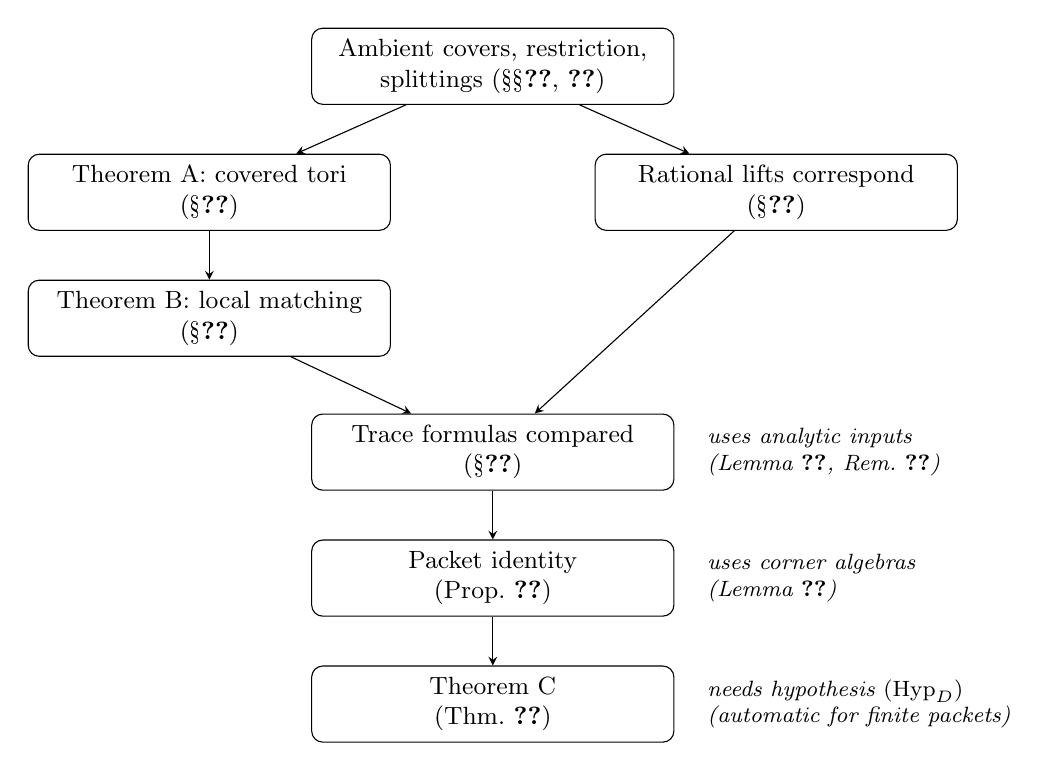
\begin{tikzpicture}[box/.style={draw,rounded corners,align=center,font=\small,inner sep=4pt,minimum width=4.6cm},ann/.style={font=\footnotesize\itshape,align=left,anchor=west},>=stealth]
\node[box] (cov) at (0,0) {Ambient covers, restriction,\\ splittings (\S\S\ref{I:sec:covers}, \ref{I:subsec:globalcovers})};
\node[box] (A) at (-3.6,-1.6) {Theorem A: covered tori\\ (\S\ref{I:sec:tori})};
\node[box] (rat) at (3.6,-1.6) {Rational lifts correspond\\ (\S\ref{I:subsec:rational})};
\node[box] (B) at (-3.6,-3.2) {Theorem B: local matching\\ (\S\ref{I:sec:matching})};
\node[box] (TF) at (0,-4.9) {Trace formulas compared\\ (\S\ref{I:sec:TF})};
\node[box] (P) at (0,-6.5) {Packet identity\\ (Prop.~\ref{I:prop:packet})};
\node[box] (C) at (0,-8.1) {Theorem C\\ (Thm.~\ref{I:thm:transfer})};
\draw[->] (cov)--(A); \draw[->] (cov)--(rat); \draw[->] (A)--(B);
\draw[->] (B)--(TF); \draw[->] (rat)--(TF); \draw[->] (TF)--(P); \draw[->] (P)--(C);
\node[ann] at (2.6,-4.9) {uses analytic inputs\\ (Lemma~\ref{I:lem:A1}, Rem.~\ref{I:rem:Einputs})};
\node[ann] at (2.6,-6.5) {uses corner algebras\\ (Lemma~\ref{I:lem:corner})};
\node[ann] at (2.6,-8.1) {needs hypothesis $(\mathrm{Hyp}_D)$\\ (automatic for finite packets)};
\end{tikzpicture}
\end{center}
Everything except the last box is unconditional, given the cited \Ev\ inputs. The \Ev\ inputs used in the global sections are listed in Remark~\ref{I:rem:Einputs}.

\subsection*{A running example}
Throughout the series we test the constructions on one case: $K=\mathbb{Q}(\zeta_3)$, $n=3$, $r=2$, $D=(-1,4-\zeta_3)_K$, which is ramified exactly at $S=\{\mathfrak p_3,\mathfrak p_7\}$, with $\mathfrak p_3=(1-\zeta_3)$ and $\mathfrak p_7=(3+\zeta_3)$. We take $L=K(i)=\mathbb{Q}(\zeta_{12})$, and $c=1$, $r'=2$, $c_v=2$ in Assumption~\ref{I:ass:standing}. At $\mathfrak p_3$, where $K_v=\mathbb{Q}_3(\zeta_3)$, the covered elliptic tori are non-abelian: the good elements have index $9$, and genuine irreducibles of a covered torus have dimension $3$ (Example~\ref{I:ex:r2n3}). At $\mathfrak p_7$, where $K_v=\mathbb{Q}_7\supset\mu_3$, they are abelian. The sign in Theorem~\ref{I:thm:easy} is $-1$. The note \texttt{notes/mjl\_running\_example.tex} in the project repository works this case out across Chapters~\ref{ch:I}--\ref{ch:IV}.

\subsection{Organization}
Section~\ref{I:sec:lit} reviews the literature for the whole series (Chapters~\ref{ch:II}--\ref{ch:IV} refer to it), and Section~\ref{I:sec:glossary} collects the notation and glossary of the series (shared by all four Parts) together with the notation specific to Chapter~\ref{ch:I}. Sections~\ref{I:sec:covers}--\ref{I:sec:matching} contain the local theory; the facts about orbital integrals on elliptic tori that it needs are proved in \S\ref{I:app:oi}. Sections~\ref{I:sec:global}--\ref{I:sec:spectral} contain the global theory, and \S\ref{I:app:cusp} supplies its analytic input for cusp forms on the cover. Section~\ref{I:sec:deferred} lists what is left after this chapter, Section~\ref{I:sec:conclusion} summarizes what the local theory gives on its own, and Section~\ref{I:sec:summary} lists the results with their labels.


% =====================================================================
\section{Local covers}\label{I:sec:covers}
This section realizes the cover of $D_v^\times$ from \cite{JC26} and the Kazhdan--Patterson cover of $\GL(r,K_v)$ as subgroups of one cover of the larger group $\GL(r,L\otimes_KK_v)$ (\S\ref{I:subsec:why}--\ref{I:subsec:ambient}). It then shows that the $\GL$-side subgroup is the Kazhdan--Patterson cover with parameter $c_v$, as an extension (\S\ref{I:subsec:restriction}), and identifies the two covers canonically at the places where $D$ splits (\S\ref{I:subsec:outsideS}). It depends only on the Kazhdan--Patterson cocycle \cite[\S0.1]{KP84}, \cite[\S2]{FK86} and the Matsumoto--Moore classification \cite{Mat69}, \cite{Moo68}, and uses from \cite{JC26} only the definition of the cover of $D_v^\times$. It introduces the ambient cover $\cGb_v$, the embeddings $\iD$ and $\iG$, the local covers $\GDb(K_v)$ and $\Gb_v$, their common central subgroup $\Zb_v$, and the identifications $\psi_v$ at $v\notin S$.

\subsection{Why an ambient cover}\label{I:subsec:why}
We explain the idea before the computations.

Equality of commutator pairings does not, by itself, give a preferred isomorphism between two central extensions. Any two isomorphisms differ by a character with values in $\mu_n$, and such characters can be nontrivial on the center. A careless choice would therefore make the comparison of central characters, and hence of genuine functions, ambiguous. Our approach is to realize both covers as \emph{subgroups} of a single cover of $\GL(r,L\otimes_KK_v)$. Conjugation in this larger group then produces isomorphisms between the relevant subgroups. These isomorphisms are in general not unique, but their restrictions to the centers of covered tori are canonical (Theorem~\ref{I:thm:ident}). Because both covers sit in one group, the common central subgroup $p^{-1}(K_v^\times)$ is literally the same subgroup on the two sides. This uses no choice of cocycle, so the question of whether two cocycles agree exactly or only up to a coboundary does not arise for it.

\subsection{The ambient cover}\label{I:subsec:ambient}
We define the ambient cover at each place and the two subgroups; the notation $\cGb_v$, $\iD$, $\iG$, $\GDb(K_v)$, $\Gb_v$, $\Zb_v$ introduced here is used throughout.

Fix once and for all an isomorphism $D\otimes_KL\cong M_r(L)$. For a place $v$ of $K$ put $L_v=L\otimes_KK_v=\prod_{w\mid v}L_w$ and $\cG_v:=\GL(r,L_v)=\prod_{w\mid v}\GL(r,L_w)$. Let $\cGb_v$ be the cover of $\cG_v$ obtained from the product of the Kazhdan--Patterson covers of the $\GL(r,L_w)$ with twisting parameter $c_v$, by identifying their copies of $\mu_n$ (i.e.\ the quotient of the product by $\{(\zeta_w):\prod_w\zeta_w=1\}$). A cocycle for $\cGb_v$ is
\begin{equation}\label{I:eq:ambient}
\prod_{w\mid v}\sigma_{L_w}(g_w,h_w)\,(\det g_w,\det h_w)_{L_w}^{c_v},
\end{equation}
where $\sigma_{L_w}$ is the Kazhdan--Patterson cocycle with parameter $0$ \cite[\S0.1]{KP84}, \cite[\S2]{FK86}. Let
\[ \iD:D_v^\times\hookrightarrow\cG_v,\qquad \iG:\GL(r,K_v)\hookrightarrow\cG_v \]
be the embedding induced by $D\otimes_KL\cong M_r(L)$, and the diagonal inclusion. Note that $\det\circ\iD=\Nrd$, and $\iD$ and $\iG$ agree on the scalars $K_v^\times$.

\begin{definition}\label{I:def:localcovers}
$\GDb(K_v):=p^{-1}(\iD(D_v^\times))\subset\cGb_v$ and $\Gb_v:=p^{-1}(\iG(\GL(r,K_v)))\subset\cGb_v$. Let $\Zb_v:=p^{-1}(K_v^\times)$; it is a subgroup of both.
\end{definition}

\begin{equation}\label{I:eq:diagram}
\begin{tikzcd}[column sep=small]
\GDb(K_v)\arrow[r,hook]\arrow[d] & \cGb_v\arrow[d] & \Gb_v\arrow[l,hook']\arrow[d]\\
D_v^\times\arrow[r,hook,"\iD"] & \GL(r,L_v) & \GL(r,K_v)\arrow[l,hook',"\iG"']
\end{tikzcd}
\qquad\qquad \Zb_v=p^{-1}(K_v^\times)\subset\GDb(K_v)\cap\Gb_v.
\end{equation}

\begin{lemma}\label{I:lem:center}\Pv
The inverse image in $\cGb_v$ of the center $L_v^\times$ of $\cG_v$ is central in $\cGb_v$. In particular $\Zb_v$ is central in $\cGb_v$, in $\GDb(K_v)$ and in $\Gb_v$.
\end{lemma}
\begin{proof}
By \cite[\S2]{FK86} (see \cite[Lemma~2.1]{JC26}), the center of the parameter-$c_v$ cover of $\GL(r,L_w)$ is the inverse image of $\{z:z^{r-1+2rc_v}\in L_w^{\times n}\}$, which is all of $L_w^\times$ since $n\mid r-1+2rc_v$. This is an \Ev\ input. Centrality in the product with identified $\mu_n$'s follows factor by factor.
\end{proof}

\subsection{The restriction lemma}\label{I:subsec:restriction}
We now identify the two subgroups of Definition~\ref{I:def:localcovers}. The $D$ side is the cover of \cite{JC26} by construction. The $\GL$ side is isomorphic, as a central extension, to the Kazhdan--Patterson cover with parameter $c_v$. This replaces the cocycle-level claim in the proof of \cite[Lemma~6.1(c)]{JC26} by a statement about extensions, with a proof that does not depend on the internal form of the Kazhdan--Patterson cocycle.

\begin{proposition}\label{I:prop:restriction}\Pv\ (using \Ev\ inputs)
Let $v$ be a finite place.
\begin{enumerate}[label=(\alph*)]
\item The pull-back of the cocycle \eqref{I:eq:ambient} along $\iD$ is the local component at $v$ of the cocycle $\beta=\sigma_L\cdot(\Nrd,\Nrd)^c$ of \cite[equation~(4)]{JC26}. Hence $\GDb(K_v)$ is the local cover of \cite[\S6.1]{JC26}.
\item There is an isomorphism of central extensions of $\GL(r,K_v)$ by $\mu_n$ (the identity on $\mu_n$ and over $\GL(r,K_v)$)
\[ \Gb_v\ \cong\ \text{the extension with cocycle }\sigma_{K_v}^{\,r}\,(\det,\det)_{K_v}^{\,c}. \]
After relabeling by $\zeta\mapsto\zeta^{r'}$, the right side is the Kazhdan--Patterson cover $\Gb^{(c_v)}$ of $\GL(r,K_v)$, normalized as in \cite[Lemma~2.1]{JC26}.
\item Any two isomorphisms as in (b) differ by an automorphism $\tilde g\mapsto\chi(\det p(\tilde g))\tilde g$ with $\chi:K_v^\times\to\mu_n$ a continuous character. Every result about $\Gb^{(c_v)}$ that we import from \cite{FK86} or \cite{KP84} is stated in terms of the group $\Gb^{(c_v)}$, the projection $p$ and $\mu_n$ alone (commutators, good elements, orbital integrals, characters, supercusp forms, germ expansions). It therefore holds for $\Gb_v$ via any such isomorphism. The only exception is the use of the splittings $\ks_v$ over maximal compact subgroups; these are defined directly on $\Gb_v$ in Proposition~\ref{I:prop:global}(d), and the local results of \cite{JC26} hold for any splitting \cite[Remarks after Lemma~6.1]{JC26}.
\end{enumerate}
\end{proposition}

\begin{proof}
(a) For $g,h\in D_v^\times$ we have $\det\iD(g)_w=\Nrd g\in K_v^\times$ for each $w\mid v$. By norm compatibility, $\prod_{w\mid v}(\Nrd g,\Nrd h)_{L_w}^{c_v}=(\Nrd g,\Nrd h)_{K_v}^{rc_v}=(\Nrd g,\Nrd h)_{K_v}^{c}$, since $\sum_w[L_w:K_v]=r$, $rc_v=rr'c\equiv c\pmod n$, and the values lie in $\mu_n$. The remaining factor is the restriction of the parameter-$0$ cocycle of $\GL(r,L_v)$, which is the local component of $\sigma_L$ in \cite[equation~(4)]{JC26}. (Globally one uses the normalized cocycle $\tau_L$ of \cite[\S2]{FK86}, which differs from the product of the $\sigma_{L_w}$ by the coboundary of $\kappa$. This changes the cocycle model of $\cGb_v$ but not the group $\cGb_v$, nor the subgroups of Definition~\ref{I:def:localcovers}.)

(b) The twisting factor restricts to $(\det,\det)_{K_v}^{c}$ exactly as in (a). So it suffices to show that, for each $w\mid v$ with $d_w:=[L_w:K_v]$, the pull-back $X_1$ of the parameter-$0$ cover of $\GL(r,L_w)$ to $\GL(r,K_v)$ is isomorphic to the extension $X_2$ with cocycle $\sigma_{K_v}^{\,d_w}$, i.e.\ the push-out of the parameter-$0$ cover of $\GL(r,K_v)$ along $\zeta\mapsto\zeta^{d_w}$. Taking the Baer sum over $w\mid v$ then gives the cocycle $\sigma_{K_v}^{\,r}$. Write $F=K_v$ and $F'=L_w$.

\emph{Step 1: the cocycles agree on the diagonal torus.} By \cite[\S2]{FK86}, the Kazhdan--Patterson cocycle restricted to the diagonal torus is $\sigma_{F'}(a,a')=\prod_{i<j}(a_i,a'_j)_{F'}$. For $a,a'\in A(F)$, norm compatibility gives $\sigma_{F'}(a,a')=\prod_{i<j}(a_i,a'_j)_F^{d_w}=\sigma_F(a,a')^{d_w}$. So the cocycles of $X_1$ and $X_2$ (in these models) agree \emph{literally} on $A(F)\times A(F)$.

\emph{Step 2: the restrictions to $\SL(r,F)$ are isomorphic.} By Matsumoto and Moore \cite{Mat69}, \cite{Moo68}, topological central extensions of $\SL(r,F)$ by $\mu_n$ are classified by continuous Steinberg symbols $c:F^\times\times F^\times\to\mu_n$. Every such symbol is $(\cdot,\cdot)_F^{k}$ for some $k\in\Z/n$ (Moore), and $\SL(r,F)$ is perfect, so an isomorphism between two extensions, if it exists, is unique \Ev. In the extension with symbol $c$, the commutator of lifts of $a,a'\in A(F)\cap\SL(r,F)$ is $\prod_ic(a_i,a'_i)^{\epsilon}$ for a universal sign $\epsilon$ \cite[\S5]{Mat69}, \cite[\S\S8--9]{Mil71} \Ev. Let $X_1|_{\SL}$ and $X_2|_{\SL}$ have symbols $(\cdot,\cdot)^{k_1}$ and $(\cdot,\cdot)^{k_2}$. Their torus commutators agree by Step~1. Take $a=\diag(x,x^{-1},1,\dots,1)$ and $a'=\diag(y,y^{-1},1,\dots,1)$; this gives $(x,y)^{2\epsilon k_1}=(x,y)^{2\epsilon k_2}$ for all $x,y$. As the Hilbert symbol is surjective onto $\mu_n$ and $n$ is odd, $k_1=k_2$. Hence the Baer difference $X:=X_1-X_2$ splits over $\SL(r,F)$, by a unique homomorphism $s:\SL(r,F)\to X$.

\emph{Step 3: $X$ splits over $\GL(r,F)$.} Let $A_1=\{\diag(a,1,\dots,1)\}\cong F^\times$, so that $\GL(r,F)=\SL(r,F)\rtimes A_1$. By Step~1 the cocycle of $X$ (the quotient of the two cocycles) is identically $1$ on $A(F)\times A(F)$, so $t(a)=(a,1)$ is a homomorphism $A_1\to X$. For $a\in A_1$, $h\mapsto t(a)s(a^{-1}ha)t(a)^{-1}$ is again a splitting of $X$ over $\SL(r,F)$, so it equals $s$ by uniqueness. Hence $S(ha):=s(h)t(a)$ ($h\in\SL(r,F)$, $a\in A_1$) is a homomorphism: $S(ha\,h'a')=s(h)\,s(ah'a^{-1})\,t(aa')=s(h)t(a)s(h')t(a)^{-1}t(a)t(a')=S(ha)S(h'a')$. So $X$ is split, i.e.\ $X_1\cong X_2$.

For the relabeling, raising $\sigma_{K_v}^{\,r}(\det,\det)_{K_v}^{\,c}$ to the power $r'$ gives $\sigma_{K_v}(\det,\det)_{K_v}^{\,c_v}$, the Kazhdan--Patterson cocycle with parameter $c_v$.

(c) Two isomorphisms of extensions over the identity differ by a continuous homomorphism $\GL(r,K_v)\to\mu_n$. Since $\SL(r,K_v)$ is perfect, such a homomorphism factors through $\det$. The rest is a remark on how the cited results are used.
\end{proof}

\begin{remark}\label{I:rem:JC61c}
(1) Proposition~\ref{I:prop:restriction}(b) is the form in which \cite[Lemma~6.1(c)]{JC26} should be stated: an isomorphism of extensions, not an equality of cocycles. The proof there, which appeals to the Bruhat decomposition, is replaced by Steps~1--3 above. An equality at the level of explicit cocycles would follow from the formula of \cite{BLS99}, where $\sigma$ is a product of Hilbert symbols of ratios of minors (which lie in $K_v$ when $g,h\in\GL(r,K_v)$); we do not need it.

(2) For $v$ split in $L$, (b) is literal: the diagonal restriction of a product of $r$ copies of a cocycle is its $r$-th power.

(3) At archimedean $v$ all Hilbert symbols are trivial, and all covers in sight are split.
\end{remark}

\begin{remark}[Central characters and the choice of isomorphism]\label{I:rem:chidet}
An isomorphism $\phi:\Gb_v\to\Gb^{(c_v)}$ as in Proposition~\ref{I:prop:restriction}(b) is determined up to twisting by $\chi\circ\det$. On the inverse image of a scalar $z$ this twist multiplies by $\chi(z^r)$. So $\phi$ transports a genuine character $\tilde\theta_v$ of $\Zb_v$ to a central character of $\Gb^{(c_v)}$ that depends on $\phi$. We avoid this ambiguity as follows.
\begin{enumerate}[label=(\arabic*)]
\item Central characters live on $\Zb_v\subset\cGb_v$ and are \emph{never} transported through $\phi$. The same $\tilde\theta_v$ serves $\GDb(K_v)$ and $\Gb_v$ (Lemma~\ref{I:lem:center}).
\item The results imported through $\phi$ are statements about all genuine functions or representations, for all central characters at once, or about objects that do not involve central characters: commutators and good elements \cite[\S3]{FK86}, convergence of orbital integrals \cite[\S6]{FK86}, supercusp forms and Selberg's principle \cite[\S13]{FK86}, Harish-Chandra's character theory, and the analytic steps of \cite[\S18]{FK86}. Such a statement for $\Gb^{(c_v)}$ with central character $\tilde\theta_v\circ\phi^{-1}$ is equivalent, via $\phi$, to the same statement for $\Gb_v$ with central character $\tilde\theta_v$. So these results hold for $\Gb_v$ independently of the choice of $\phi$.
\item Results tied to a normalized identification are \emph{not} used in Chapter~\ref{ch:I}. These include the unramified theory relative to the splitting of \cite{KP84}, the Flicker--Kazhdan correspondence relating specific central characters of $\Gb^{(c_v)}$ and $\GL(r,K_v)$, and exceptional representations. For the later parts we note the following. For almost all $v$, two splittings over $\GL(r,\cO_v)$ differ by $\chi_0\circ\det$ with $\chi_0$ a character of $\cO_v^\times$. Extending $\chi_0$ to $K_v^\times$, one can choose $\phi$ to carry $\ks_v$ of Proposition~\ref{I:prop:global}(d) to the Kazhdan--Patterson splitting. Such $\phi$ are then unique up to $\chi\circ\det$ with $\chi$ unramified, and the remaining ambiguity on $\Zb_v$ is $\chi(\varpi^r)\in\mu_n$, which must be fixed separately when the Flicker--Kazhdan correspondence is applied.
\end{enumerate}
\end{remark}

\subsection{Places where $D$ splits}\label{I:subsec:outsideS}
At $v\notin S$ the groups $D_v^\times$ and $\GL(r,K_v)$ are isomorphic. We show that the corresponding covers are identified by conjugation in $\cGb_v$, canonically once the isomorphism of the base groups is fixed, and compatibly with the splittings over maximal compact subgroups at almost all places. This is step~(2) of \cite[Remark~10.3]{JC26}.

\begin{proposition}\label{I:prop:outsideS}\Pv
Let $v\notin S$ and fix a $K_v$-algebra isomorphism $\alpha_v:D_v\xrightarrow{\sim}M_r(K_v)$.
\begin{enumerate}[label=(\alph*)]
\item There is $g_v\in\cG_v$ with $\Ad(g_v)\circ\iD=\iG\circ\alpha_v$ on $D_v^\times$. It is unique up to the center $L_v^\times$ of $\cG_v$.
\item $\psi_v:=\Ad(\tilde g_v)|_{\GDb(K_v)}:\GDb(K_v)\to\Gb_v$ (any lift $\tilde g_v$) is an isomorphism of covers over $\alpha_v$. It is the identity on $\mu_n$ and on $\Zb_v$, and depends only on $\alpha_v$. Replacing $\alpha_v$ by $\Ad(h)\circ\alpha_v$ with $h\in\GL(r,K_v)$ replaces $\psi_v$ by $\Ad(\tilde h)\circ\psi_v$.
\item Suppose $v$ is finite, $v\nmid n$, $\alpha_v(\cO_{D,v})=M_r(\cO_v)$ for the global order $\cO_D$ used in \cite[Lemma~6.1(d)]{JC26}, and $\iD(\cO_{D,v})\otimes\cO_{L_v}=M_r(\cO_{L_v})$ (true for almost all $v$). Then $g_v$ may be taken in $\GL(r,\cO_{L_v})$, and $\psi_v$ carries the splitting $\ks_v(G_D(\cO_v))$ of \cite[Lemma~6.1(d)]{JC26} to the splitting $\ks_v(\GL(r,\cO_v))$ of Proposition~\ref{I:prop:global}(d).
\end{enumerate}
\end{proposition}
\begin{proof}
(a) Both $\iD$ and $\iG\circ\alpha_v$ extend $L_v$-linearly to $L_v$-algebra isomorphisms $D_v\otimes_{K_v}L_v\to M_r(L_v)$, so they differ by an $L_v$-algebra automorphism of $M_r(L_v)=\prod_wM_r(L_w)$. Such an automorphism preserves the idempotents of $L_v$, hence each factor, and on each factor it is inner (Skolem--Noether). Uniqueness up to the centralizer of $\iG(M_r(K_v))\otimes L_v=M_r(L_v)$, which is $L_v^\times$, is clear.

(b) $\Ad(\tilde g_v)$ is an automorphism of $\cGb_v$, trivial on $\mu_n$, over $\Ad(g_v)$, so it maps $p^{-1}\iD(D_v^\times)$ onto $p^{-1}\iG(\GL(r,K_v))$. Changing $\tilde g_v$ within $p^{-1}(g_vL_v^\times)$ does not change $\Ad(\tilde g_v)$, since $p^{-1}(L_v^\times)$ is central (Lemma~\ref{I:lem:center}). The same lemma shows $\psi_v$ is the identity on $\Zb_v$. The last assertion is clear.

(c) Under the hypotheses, $\Ad(g_v)$ restricts to an automorphism of the Azumaya algebra $M_r(\cO_{L_v})$ over $\cO_{L_v}=\prod_w\cO_{L_w}$, a product of local rings. Such an automorphism is inner by an element of $\GL(r,\cO_{L_v})$ (Skolem--Noether for Azumaya algebras over local rings, whose Picard groups are trivial). So $g_v\in L_v^\times\GL(r,\cO_{L_v})$, and we may take $g_v\in\GL(r,\cO_{L_v})$. The splittings in question are the restrictions of the splitting $\ks_{\cG_v}$ of $\cGb_v$ over $\GL(r,\cO_{L_v})$ (Proposition~\ref{I:prop:global}(d) and \cite[Lemma~6.1(d)]{JC26}). Since $\ks_{\cG_v}$ is a homomorphism, $\Ad(\ks_{\cG_v}(g_v))$ carries $\ks_{\cG_v}(\iD(k))$ to $\ks_{\cG_v}(g_v\iD(k)g_v^{-1})=\ks_{\cG_v}(\iG\alpha_v(k))$.
\end{proof}

% =====================================================================
\section{Comparison of covered elliptic tori at the ramified places}\label{I:sec:tori}
This section shows that, at a place $v\in S$, the covered torus $\Eb_D\subset\GDb(K_v)$ attached to a maximal subfield $E\subset D_v$ and the covered torus $\Eb_{\GL}\subset\Gb_v$ attached to an embedding $E\hookrightarrow M_r(K_v)$ have the same commutator pairing, the same good elements and the same centers. They are identified on good elements by a canonical isomorphism. We compute the pairing (\S\ref{I:subsec:comm}) and the good elements (\S\ref{I:subsec:good}), give an example (\S\ref{I:subsec:example}), construct the identification (\S\ref{I:subsec:ident}), and record its consequences (\S\ref{I:subsec:cons}). It depends on \S\ref{I:sec:covers} (Lemma~\ref{I:lem:center} and Proposition~\ref{I:prop:restriction}) and on the commutator formula of \cite[\S3]{FK86}, \cite[Prop.~0.1.5]{KP84}. It introduces the covered tori $\Eb_D$ and $\Eb_{\GL}$, the set $\Iso_{\Zb}(\Eb_D,\Eb_{\GL})$, the canonical identification $\jj_{E,j}$ and the induced bijection $\jj$ of good regular elliptic classes.

Throughout this section, $v\in S$, $F:=K_v$, $w$ is the unique place of $L$ over $v$, so that $\cG_v=\GL(r,L_w)$, and $L_w/F$ is cyclic of degree $r$. Let $E\subset D_v$ be a maximal subfield, so $[E:F]=r$, and let $j:E\hookrightarrow M_r(F)$ be an $F$-algebra embedding. (One exists, e.g.\ the regular representation; any two are $\GL(r,F)$-conjugate.) We write $N=N_{E/F}$, $\Eb_D:=p^{-1}(\iD(E^\times))\subset\GDb(K_v)$ and $\Eb_{\GL}:=p^{-1}(\iG j(E^\times))\subset\Gb_v$.

\subsection{The commutator pairings}\label{I:subsec:comm}
We compute the commutator pairing of the covered torus on each side, inside $\cGb_v$, and find the same answer.

For $x,y\in E^\times$ write $[x,y]_D$ and $[x,y]_{\GL}$ for the commutators of lifts of $\iD(x),\iD(y)$ and of $\iG j(x),\iG j(y)$. They are well defined and bimultiplicative \cite[\S3]{FK86}.

\begin{proposition}\label{I:prop:comm}\Pv
For all $x,y\in E^\times$,
\begin{equation}\label{I:eq:commboth}
[x,y]_D=[x,y]_{\GL}=(Nx,Ny)_F^{\,r+2c}\,(x,y)_E^{-r}\qquad\text{(before relabeling)}.
\end{equation}
After relabeling by $\zeta\mapsto\zeta^{r'}$ this becomes
\begin{equation}\label{I:eq:commrelab}
[x,y]=(Nx,Ny)_F^{\,1+2c_v}\,(x,y)_E^{-1}=\big((Nx)^{1+2c_v}x^{-1},\,y\big)_E,
\end{equation}
which is \cite[equation~(2)]{JC26} for the elliptic torus $j(E^\times)$ of $\Gb^{(c_v)}$.
\end{proposition}

\begin{proof}
Commutators are invariants of the extension, so we may compute in any model. We use the formula of \cite[\S3]{FK86} and \cite[Prop.~0.1.5]{KP84} \Ev: for a maximal torus $T'=\prod_iF_i'^\times$ of $\GL(r,F')$ and the parameter-$0$ cover, $[x,y]=(\det x,\det y)_{F'}\prod_i(x_i,y_i)_{F_i'}^{-1}$. Twisting by $(\det,\det)^{m}$ multiplies commutators by $(\det x,\det y)^{2m}$.

\emph{The $D$ side.} $\iD(x),\iD(y)$ lie in the maximal torus $\iD(E\otimes_FL_w)^\times$ of $\cG_v$. Write $E\otimes_FL_w=\prod_iE_i$ with fields $E_i\supseteq E$; then $\sum_i[E_i:L_w]=r$, and $[E_i:E]=[E_i:L_w]$ since $[E:F]=[L_w:F]$. We have $\det\iD(x)=Nx\in F^\times$, so
\[ (\det x,\det y)_{L_w}=(Nx,Ny)_F^{\,r},\qquad \prod_i(x,y)_{E_i}=\prod_i(x,N_{E_i/E}\,y)_E=(x,y)_E^{\,r}. \]
The twist by $(\det,\det)_{L_w}^{c_v}$ contributes $(Nx,Ny)_F^{2rc_v}=(Nx,Ny)_F^{2c}$.

\emph{The $\GL$ side.} By Proposition~\ref{I:prop:restriction}(b) the extension $\Gb_v$ has cocycle $\sigma_F^r(\det,\det)_F^c$ up to isomorphism. For the parameter-$0$ cover and the elliptic torus $j(E^\times)$, \cite[\S3]{FK86} gives $(Nx,Ny)_F(x,y)_E^{-1}$. Raising to the $r$-th power and multiplying by $(Nx,Ny)_F^{2c}$ gives the same expression.

\emph{Relabeling.} Raise \eqref{I:eq:commboth} to the power $r'$. For the last equality in \eqref{I:eq:commrelab}, $(Nx,Ny)_F=(Nx,y)_E$ by norm compatibility, since $Nx\in F^\times$.
\end{proof}

\begin{remark}\label{I:rem:robust}
The equality $[x,y]_D=[x,y]_{\GL}$ uses the formula of \cite[\S3]{FK86} only through its multiplicative shape. If the formula were $(\det x,\det y)^{a}\prod_i(x_i,y_i)^{b}$, both sides of \eqref{I:eq:commboth} would become $(Nx,Ny)_F^{ra+2c}(x,y)_E^{rb}$.
\end{remark}

\begin{remark}[The twisting parameter is forced]\label{I:rem:forced}
If the $\GL$-side cover had parameter $c'$ instead of $c_v$, its pairing on $j(E^\times)$ would be $(Nx,Ny)_F^{1+2c'}(x,y)_E^{-1}$. This agrees with \eqref{I:eq:commrelab} if and only if $(Nx,Ny)_F^{2(c'-c_v)}=1$ for all $x,y\in E^\times$. Since $N(E^\times)\supseteq F^{\times r}$ and $(F^{\times r},F^{\times r})_F=\mu_n$, and $n$ is odd, this holds if and only if $c'\equiv c_v\pmod n$. So matching requires exactly $\Gb^{(c_v)}$, compared with the $D$ side through the same relabeling of $\mu_n$.
\end{remark}

\subsection{Good elements and centers}\label{I:subsec:good}
From the explicit pairing we determine the good elements on both sides, the index of the center, and hence the dimension of genuine irreducible representations of the covered torus.

\begin{lemma}\label{I:lem:FcapEn}\Pv
$F^\times\cap E^{\times n}=F^{\times n}$. Hence $F^\times/F^{\times n}\to E^\times/E^{\times n}$ is injective.
\end{lemma}
\begin{proof}
If $z=y^n$ with $y\in E^\times$, then $z^r=N(z)=N(y)^n\in F^{\times n}$. Also $z^n\in F^{\times n}$, and $(r,n)=1$, so $z\in F^{\times n}$.
\end{proof}

\begin{proposition}\label{I:prop:good}\Pv
Let $\bullet\in\{D,\GL\}$.
\begin{enumerate}[label=(\alph*)]
\item An element $\tilde x\in\Eb_\bullet$ is good (central in $\Eb_\bullet$) if and only if $p(\tilde x)\in F^\times E^{\times n}$. No regularity assumption is needed.
\item $[\Eb_\bullet:Z(\Eb_\bullet)]=[E^\times:F^\times E^{\times n}]=|n|_F^{-(r-1)}$. In particular $\Eb_\bullet$ is abelian if and only if $v\nmid n$.
\item Every genuine irreducible smooth representation of $\Eb_\bullet$ has dimension $|n|_F^{-(r-1)/2}$ (an integer: if $p\mid n$ and $p^k\Vert n$, then $\mu_{p^k}\subset F$ forces $p-1\mid[F:\mathbb Q_p]$, so $|n|_F^{-1}=p^{k[F:\mathbb Q_p]}$ is a square), and is determined by its central character on $Z(\Eb_\bullet)$ \cite[Prop.~2.4]{JC26}.
\item If $x\in E^\times\smallsetminus F^\times$, then $F(x^n)=E$. In particular, if $x$ is regular, so is $x^n$.
\end{enumerate}
\end{proposition}

\begin{proof}
(a) By \eqref{I:eq:commrelab}, $\tilde x$ is central if and only if $((Nx)^{1+2c_v}x^{-1},y)_E=1$ for all $y\in E^\times$. By nondegeneracy of the Hilbert symbol, this holds if and only if $x\equiv(Nx)^{1+2c_v}\pmod{E^{\times n}}$. If so, $x\in F^\times E^{\times n}$. Conversely, if $x=zy^n$ with $z\in F^\times$, then $(Nx)^{1+2c_v}\equiv z^{r(1+2c_v)}=z\cdot z^{r-1+2rc_v}\equiv z\equiv x\pmod{E^{\times n}}$.

(b) Since $\mu_n\subset F$, we have $|F^\times/F^{\times n}|=n^2|n|_F^{-1}$ and $|E^\times/E^{\times n}|=n^2|n|_E^{-1}=n^2|n|_F^{-r}$ \cite[Ch.~II, \S5]{Neu99} \Ev. Now use Lemma~\ref{I:lem:FcapEn}.

(c) Stone--von Neumann: the dimension is the square root of the index.

(d) Put $F'=F(x^n)\subseteq E$. Since $\mu_n\subset F'$, the degree of the Kummer extension $F'(x)/F'$ divides $n$. It also divides $r$, so it is $1$. As $r$ is prime and $x\notin F$, $F(x)=E$, so $F'=E$.
\end{proof}

\begin{remark}
Part~(b) generalizes \cite[Lemma~2.5]{JC26} from unramified $E$ to all maximal subfields when $v\nmid n$. Part~(d) shows that for regular elliptic elements the condition ``$x^*$ regular'' in \cite[\S18]{FK86} is automatic.
\end{remark}

\subsection{An example}\label{I:subsec:example}
We illustrate the index computation with the smallest case in which a place above $n$ makes the covered torus non-abelian.

\begin{example}\label{I:ex:r2n3}
Take $r=2$, $n=3$, and $F=K_v=\Q_3(\zeta_3)$, so $D_v$ is the quaternion division algebra over $F$. We may take $c=1$ (so $3\mid r-1+2c=3$), $r'=2$ and $c_v=2$, and indeed $3\mid r-1+2rc_v=9$. For any quadratic extension $E/F$, \eqref{I:eq:commrelab} reads $[x,y]=(Nx,Ny)_F^{5}(x,y)_E^{-1}=(Nx,Ny)_F^{2}(x,y)_E^{-1}$. The field $F$ is totally ramified of degree $2$ over $\Q_3$, so $|3|_F=3^{-2}$ and
\[ [\Eb:Z(\Eb)]=|3|_F^{-1}=9. \]
So every genuine irreducible representation of $\Eb_D$ or $\Eb_{\GL}$ has dimension $3$, and the good elements form a subgroup of index $9$ in $E^\times$. (As a check, $|F^\times/F^{\times3}|=3\cdot3\cdot9=81$.) By contrast, at a place $v\in S$ of residual characteristic $\ne3$, every covered elliptic torus is abelian.
\end{example}

\subsection{A canonical identification on good elements}\label{I:subsec:ident}
Equal commutator pairings leave open whether the two covered tori are isomorphic, and if so how canonically. We show that they are isomorphic, by conjugation inside $\cGb_v$, and that every isomorphism that is the identity on the common central subgroup $\Zb_v$ has the same restriction to good elements. This defines the identification $\jj_{E,j}$ used in the rest of the paper.

\begin{definition}
Let $\Iso_{\Zb}(\Eb_D,\Eb_{\GL})$ be the set of isomorphisms of topological groups $\varphi:\Eb_D\to\Eb_{\GL}$ with $p\circ\varphi=(\iG j\iD^{-1})\circ p$ that are the identity on $\mu_n$ and on $\Zb_v$.
\end{definition}

\begin{theorem}\label{I:thm:ident}\Pv
\begin{enumerate}[label=(\alph*)]
\item There is $g\in\cG_v$ with $g\,\iD(e)\,g^{-1}=\iG(j(e))$ for all $e\in E$. For any lift $\tilde g$, $\Ad(\tilde g)$ restricts to an element $\varphi_g\in\Iso_{\Zb}(\Eb_D,\Eb_{\GL})$.
\item Any two elements of $\Iso_{\Zb}(\Eb_D,\Eb_{\GL})$ agree on $Z(\Eb_D)$. The common restriction
\[ \jj_{E,j}:Z(\Eb_D)\xrightarrow{\ \sim\ }Z(\Eb_{\GL}) \]
is an isomorphism and a homeomorphism. It is the identity on $\Zb_v$, satisfies $p\circ\jj_{E,j}=(\iG j\iD^{-1})\circ p$, commutes with $n$-th powers, and preserves regularity.
\item $\Iso_{\Zb}(\Eb_D,\Eb_{\GL})$ is a torsor under the group of continuous characters $E^\times\to\mu_n$ trivial on $F^\times$; all of these are trivial on $F^\times E^{\times n}$.
\end{enumerate}
\end{theorem}

\begin{proof}
(a) Via $\iD$ and $\iG\circ j$, the space $L_w^r$ is a module over the \'etale $L_w$-algebra $A:=E\otimes_FL_w=\prod_iE_i$, faithful in both cases. A faithful $A$-module of $L_w$-dimension $r=\dim_{L_w}A$ is free of rank one, since each $E_i$ must act nontrivially and dimensions add up. So the two module structures are conjugate by some $g\in\cG_v$. Then $\Ad(\tilde g)$ is an automorphism of $\cGb_v$ over $\Ad(g)$, trivial on $\mu_n$, mapping $\Eb_D$ onto $\Eb_{\GL}$. It is the identity on $\Zb_v$ by Lemma~\ref{I:lem:center}, and it is continuous with continuous inverse.

(b) If $\varphi,\varphi'\in\Iso_{\Zb}$, then $\varphi'\varphi^{-1}$ is an automorphism of $\Eb_{\GL}$ over the identity, trivial on $\mu_n$, so it is $\tilde x\mapsto\chi(x)\tilde x$ for a continuous character $\chi:E^\times\to\mu_n$. Then $\chi|_{F^\times}=1$, and $\chi$ is trivial on $E^{\times n}$ since it has values in $\mu_n$. So $\varphi=\varphi'$ on $p^{-1}(F^\times E^{\times n})=Z(\Eb_D)$ (Proposition~\ref{I:prop:good}(a)). The other properties hold for any $\varphi$, and $\varphi_g$ is a homeomorphism by (a).

(c) This is the computation in (b), together with the fact that $\tilde x\mapsto\chi(x)\tilde x$ is an automorphism for every such $\chi$.
\end{proof}

\begin{equation}\label{I:eq:toridiagram}
\begin{tikzcd}
Z(\Eb_D)\arrow[r,"\jj_{E,j}","\sim"']\arrow[d,"p"'] & Z(\Eb_{\GL})\arrow[d,"p"]\\
F^\times E^{\times n}\arrow[r,"="] & F^\times E^{\times n}
\end{tikzcd}
\qquad\text{(identity on }\Zb_v\text{, on the bottom identified via }\iD,\ \iG\circ j).
\end{equation}

\begin{remark}
Off the good elements, $\varphi$ depends on choices through a character of $E^\times/F^\times E^{\times n}$, a group that is nontrivial exactly when $v\mid n$. This does no harm, since genuine orbital integrals vanish at non-good elements (\S\ref{I:sec:matching}) and genuine representations of covered tori are determined by their central characters.
\end{remark}

\subsection{Consequences}\label{I:subsec:cons}
We record that the identification is natural for conjugation, independent of $j$, and induces bijections of good regular elliptic classes and of genuine representations of covered tori. The class sets $\mathcal C^{g}(\GDb(K_v))$, $\mathcal C^{g}_{\mathrm{ell}}(\Gb_v)$ and the bijection $\jj$ defined here enter the definition of matching in \S\ref{I:sec:matching}.

\begin{proposition}[Naturality]\label{I:prop:natural}\Pv
Let $y\in D_v^\times$ and $h\in\GL(r,F)$, and put $E'=yEy^{-1}$ and $j'=\Ad(h)\circ j\circ\Ad(y)^{-1}:E'\hookrightarrow M_r(F)$. Then on $Z(\Eb_D)$
\[ \jj_{E',j'}\circ\Ad(\tilde y)=\Ad(\tilde h)\circ\jj_{E,j}. \]
In particular $\jj_{E,j}$ depends on $j$ only through its $\GL(r,F)$-conjugacy class, which is unique. If $y$ normalizes $E$ and $h$ normalizes $j(E)$, inducing the same automorphism of $E$, then $\jj_{E,j}\circ\Ad(\tilde y)=\Ad(\tilde h)\circ\jj_{E,j}$.
\end{proposition}
\begin{proof}
Put $j_1:=\Ad(h)\circ j=j'\circ\Ad(y)$. Let $\varphi\in\Iso_{\Zb}(\Eb_D,\Eb_{\GL})$ and $\varphi'\in\Iso_{\Zb}(\Eb'_D,\Eb'_{\GL})$, relative to $j$ and $j'$. Then $\Ad(\tilde h)\circ\varphi$ and $\varphi'\circ\Ad(\tilde y)$ are isomorphisms $\Eb_D\to\Eb'_{\GL}$ over $j_1$. Both are the identity on $\mu_n$ and on the central subgroup $\Zb_v$ (Lemma~\ref{I:lem:center}). By Theorem~\ref{I:thm:ident}(b) for $j_1$, they agree on $Z(\Eb_D)$.
\end{proof}

A regular element $\tilde\gamma$ of $\GDb(K_v)$ or $\Gb_v$ is \emph{good} if it is central in $\ov{T_\gamma}$, where $T_\gamma$ is the centralizer of $\gamma=p(\tilde\gamma)$. Let $\mathcal C^{g}(\GDb(K_v))$ be the set of conjugacy classes of good regular elements of $\GDb(K_v)$ (all regular elements of $D_v^\times$ are elliptic), and $\mathcal C^{g}_{\mathrm{ell}}(\Gb_v)$ the set of conjugacy classes of good regular elliptic elements of $\Gb_v$.

\begin{corollary}\label{I:cor:classes}\Pv
The maps $\jj_{E,j}$ induce a well-defined bijection
\[ \jj:\mathcal C^{g}(\GDb(K_v))\xrightarrow{\ \sim\ }\mathcal C^{g}_{\mathrm{ell}}(\Gb_v),\qquad [\tilde\gamma]\mapsto[\jj_{F(\gamma),j}(\tilde\gamma)]. \]
It preserves (reduced) characteristic polynomials and commutes with multiplication by $\Zb_v$.
\end{corollary}
\begin{proof}
\emph{Well defined:} by Proposition~\ref{I:prop:natural}. \emph{Surjective:} if $\tilde\gamma'$ is good regular elliptic, $E'=F(p(\tilde\gamma'))$ is a field of degree $r$, which embeds in $D_v$ \cite[Ch.~XIII]{Wei73}. Choose $E\subset D_v$ and $j$ with $j(E)=E'$; then $\tilde\gamma'\in Z(\Eb_{\GL})$ is $\jj_{E,j}$ of a unique element. \emph{Injective:} if $\jj(\tilde\gamma_1)$ and $\jj(\tilde\gamma_2)$ are conjugate, then $p(\tilde\gamma_1)$ and $p(\tilde\gamma_2)$ have the same characteristic polynomial, hence are conjugate in $D_v^\times$. By naturality we may assume $p(\tilde\gamma_1)=p(\tilde\gamma_2)$, so $\tilde\gamma_2=\zeta\tilde\gamma_1$ with $\zeta\in\mu_n$ and $\zeta\jj(\tilde\gamma_1)$ is conjugate to $\jj(\tilde\gamma_1)$. If $x^{-1}\tilde\delta x=\zeta\tilde\delta$ with $\tilde\delta$ regular and good, then $p(x)$ centralizes $p(\tilde\delta)$, so $x\in\ov{T_\delta}$ commutes with $\tilde\delta$, and $\zeta=1$.
\end{proof}

\begin{corollary}\label{I:cor:reps}\Pv
For $\varphi\in\Iso_{\Zb}(\Eb_D,\Eb_{\GL})$, $\chi\mapsto\chi\circ\varphi^{-1}$ induces a bijection between isomorphism classes of genuine irreducible smooth representations of $\Eb_D$ and $\Eb_{\GL}$, independent of $\varphi$. On good elements $\tr\chi(\tilde t)=\tr(\chi\circ\varphi^{-1})(\jj_{E,j}(\tilde t))$, and both characters vanish off the good elements.
\end{corollary}
\begin{proof}
By \cite[Prop.~2.4]{JC26} the isomorphism class is determined by the central character $\zeta_\chi$ on $Z(\Eb_\bullet)$, and the central character of $\chi\circ\varphi^{-1}$ is $\zeta_\chi\circ\jj_{E,j}^{-1}$, independent of $\varphi$ by Theorem~\ref{I:thm:ident}(b).
\end{proof}

% =====================================================================
\section{Orbital integrals and matching}\label{I:sec:matching}
This section defines normalized orbital integrals of genuine functions and the notion of matching (\S\S\ref{I:subsec:oi}--\ref{I:subsec:defmatch}). It then proves that matching functions exist, in both directions, for functions supported on the regular set (\S\S\ref{I:subsec:transported}--\ref{I:subsec:easy}). Finally it explains exactly what fails for general functions (\S\ref{I:subsec:general}). The last subsection, \S\ref{I:app:oi}, proves the facts about orbital integrals on elliptic tori that the section uses. It depends on \S\ref{I:sec:tori}. It introduces the normalized orbital integrals $\Phi$ and $F=\Delta\Phi$, the matching conditions (M1)--(M2), the representatives $E_i$, $j_i$, $\jj_i$ of elliptic tori, and admissible functions on covered tori. Throughout, $v\in S$ and $F=K_v$, and $\tilde\theta_v$ is a genuine character of $\Zb_v$; by Lemma~\ref{I:lem:center} the same character serves both sides.

\subsection{Orbital integrals and measures}\label{I:subsec:oi}
We fix measures, define the normalized orbital integrals, and record their basic properties. The representatives $E_i$, $j_i$, $\jj_i$ and the measures $dg_D$, $dg$, $dt_i$ fixed here are used in the rest of the paper.

\emph{Representatives of tori.} The field extensions of $F$ of degree $r$ fall into finitely many isomorphism classes; fix representatives $E_1,\dots,E_m$. For each $i$ fix an embedding $E_i\subset D_v$ (it exists \cite[Ch.~XIII]{Wei73}) and an embedding $j_i:E_i\hookrightarrow M_r(F)$. Every maximal subfield of $D_v$ is $D_v^\times$-conjugate to exactly one $E_i$, and every elliptic maximal torus of $\GL(r,F)$ is conjugate to exactly one $j_i(E_i^\times)$ (Skolem--Noether). Write $\jj_i:=\jj_{E_i,j_i}$.

\emph{Measures.} Fix Haar measures $dg_D$ on $D_v^\times/F^\times$ and $dg$ on $\GL(r,F)/F^\times$, and for each $i$ a Haar measure $dt_i$ on $E_i^\times/F^\times$. Use $dt_i$ on both $\iD(E_i^\times)/F^\times$ and $j_i(E_i^\times)/F^\times$, and transport it by conjugation to every torus conjugate to these. Quotient measures on $T\backslash G$ are $dg/dt$. The matching relation below does not depend on the choice of the $dt_i$: rescaling $dt_i$ by $\lambda$ multiplies the orbital integrals on both sides at elements of tori of type $i$ by $\lambda^{-1}$. It does depend on $dg_D$ and $dg$, which are fixed.

\begin{definition}\label{I:def:oi}
For $\bullet\in\{D,\GL\}$, $G_\bullet\in\{D_v^\times,\GL(r,F)\}$, a genuine $\tilde f\in C_c^\infty(\ov{G_\bullet},\tilde\theta_v)_\gen$ and a good regular semisimple $\tilde\gamma$ with centralizer $T_\gamma$, put
\[ \Phi(\tilde\gamma,\tilde f):=\int_{T_\gamma\backslash G_\bullet}\tilde f(\tilde x^{-1}\tilde\gamma\tilde x)\,d\dot x,\qquad F(\tilde\gamma,\tilde f):=\Delta(\gamma)\,\Phi(\tilde\gamma,\tilde f), \]
with $\Delta(\gamma)=|D(\gamma)|_F^{1/2}|\det\gamma|_F^{-(r-1)/2}$ as in \cite[\S6]{FK86}, where $D(\gamma)$ is the discriminant of the (reduced) characteristic polynomial and $\det=\Nrd$ on the $D$ side. For non-good regular $\tilde\gamma$ put $F(\tilde\gamma,\tilde f):=0$.
\end{definition}

\begin{lemma}\label{I:lem:oiprops}\Pv\ (convergence: \Ev)
\begin{enumerate}[label=(\alph*)]
\item The integrand of $\Phi$ is independent of the lift $\tilde x$ and left $T_\gamma$-invariant (because $\tilde\gamma$ is good). The integral converges absolutely. On the $D$ side $T_\gamma\backslash D_v^\times$ is compact, since $D_v^\times/F^\times$ is. On the $\GL$ side the orbit of a regular semisimple element is closed, and convergence is \cite[\S6]{FK86} (following Rao) \Ev.
\item $F(\cdot,\tilde f)$ is constant on conjugacy classes, and $F(z\tilde\gamma,\tilde f)=\tilde\theta_v(z)^{-1}F(\tilde\gamma,\tilde f)$ for $z\in\Zb_v$; in particular it is genuine.
\item If $\tilde\gamma$ is regular elliptic and not good, then the formal integral $\int_{T_\gamma\backslash G_\bullet}$ (over $\ov{T_\gamma}\backslash\ov{G_\bullet}$) vanishes; this is \cite[Prop.~2.7]{JC26} with $\eps=1$. Thus the convention $F=0$ at non-good elements loses nothing.
\item For $\gamma\in E_i^\times$ regular, $\Delta(\gamma)$ is the same on the two sides. If $E_i/F$ is cyclic, then $\Delta$ equals $|t_0^2|_F^{1/2}$ times the factor $\Delta$ of \cite[\S4.1]{JC26} with $\eps=1$, for any $t_0$ as there, so that $F(\cdot,\tilde f)=|t_0^2|_F^{1/2}\,\tilde f^{T}$ in the notation of \cite[\S4.1]{JC26}.
\end{enumerate}
\end{lemma}
\begin{proof}
(a) and (b) are immediate from the definitions, Lemma~\ref{I:lem:center} and conjugation invariance of the measures. (c) is \cite[Prop.~2.7]{JC26}. (d) The characteristic polynomials agree. For \cite{JC26}'s factor (defined only for cyclic $E_i$): $\tilde\Delta(t)^2=\pm D(t)$ and $t_0^2\in F^\times$, so $|\tilde\Delta(t)t_0^{-1}|_F=|D(t)|_F^{1/2}|t_0^2|_F^{-1/2}$.
\end{proof}

\subsection{Definition of matching}\label{I:subsec:defmatch}
We define matching with the sign $(-1)^{r-1}$ and with vanishing at good regular non-elliptic elements, using the bijection of Corollary~\ref{I:cor:classes}.

\begin{definition}\label{I:def:matching}
Functions $\tilde f_D\in C_c^\infty(\GDb(K_v),\tilde\theta_v)_\gen$ and $\tilde f\in C_c^\infty(\Gb_v,\tilde\theta_v)_\gen$ \emph{match} if
\begin{enumerate}[label=(M\arabic*)]
\item $F(\tilde\gamma,\tilde f_D)=(-1)^{r-1}F(\jj(\tilde\gamma),\tilde f)$ for every good regular $\tilde\gamma\in\GDb(K_v)$, and
\item $F(\tilde\delta,\tilde f)=0$ for every good regular non-elliptic $\tilde\delta\in\Gb_v$.
\end{enumerate}
\end{definition}

By Corollary~\ref{I:cor:classes} and Lemma~\ref{I:lem:oiprops}(b), (M1) is a condition on conjugacy classes, and it is compatible with the common central character $\tilde\theta_v$. With the sign placed here, the expected character relation $\Theta_{\pib_D}=(-1)^{r-1}\Theta_{\pib}\circ\jj$ on good regular elements would give $\tr\pib_D(\tilde f_D)=\tr\pib(\tilde f)$ for matching functions. Badulescu \cite[\S4.6]{Bad08} puts no sign in the matching of functions and keeps the sign $(-1)^{nd-n}$ in the character relation; the two conventions are equivalent.

\subsection{Transported orbital-integral functions}\label{I:subsec:transported}
We show that the orbital integrals of a regular-supported function on one side, transported to the other side by the identifications $\jj_i$, have exactly the properties that characterize orbital integrals of regular-supported functions there. The proofs, for arbitrary (not necessarily cyclic) maximal subfields, are in \S\ref{I:app:oi}. The notion of an admissible function defined here is used again in \S\ref{I:app:oi}.

For $\bullet\in\{D,\GL\}$ and each $i$, let $\Eb_{i,\bullet}$ be the covered torus of type $i$ (Definition in \S\ref{I:sec:tori}, with $E=E_i$, $j=j_i$), $Z(\Eb_{i,\bullet})^{\reg}$ its good regular elements, and $W_{i,\bullet}:=N_{G_\bullet}(T_{i,\bullet})/T_{i,\bullet}$, which acts on $Z(\Eb_{i,\bullet})$ by conjugation and injects into $\Aut(E_i/F)$. Call a function $h$ on $Z(\Eb_{i,\bullet})^{\reg}$ \emph{admissible} if
\begin{enumerate}[label=(\roman*)]
\item $h$ is locally constant;
\item $h(z\tilde t)=\tilde\theta_v(z)^{-1}h(\tilde t)$ for $z\in\Zb_v$ (in particular $h$ is genuine);
\item the support of $h$ is compact modulo $\Zb_v$ and contained in $Z(\Eb_{i,\bullet})^{\reg}$, i.e.\ its closure in $Z(\Eb_{i,\bullet})$ avoids the non-regular elements;
\item $h(\tilde y\tilde t\tilde y^{-1})=h(\tilde t)$ for $y\in N_{G_\bullet}(T_{i,\bullet})$.
\end{enumerate}

\begin{lemma}\label{I:lem:transported}\Pv
\begin{enumerate}[label=(\alph*)]
\item If $\tilde f\in C_c^\infty(\ov{G_\bullet},\tilde\theta_v)_\gen$ is supported in the regular set, then for each $i$ the restriction of $F(\cdot,\tilde f)$ to $Z(\Eb_{i,\bullet})^{\reg}$ is admissible.
\item $h\mapsto h\circ\jj_i^{-1}$ is a bijection from admissible functions on $Z(\Eb_{i,D})^{\reg}$ to admissible functions on $Z(\Eb_{i,\GL})^{\reg}$.
\item Conversely, every admissible $h$ on $Z(\Eb_{i,\bullet})^{\reg}$ is of the form $F(\cdot,\tilde f_i)|_{Z(\Eb_{i,\bullet})^{\reg}}$ for some $\tilde f_i\in C_c^\infty(\ov{G_\bullet},\tilde\theta_v)_\gen$ supported on the set of $G_\bullet$-conjugates of $\supp h$. In particular $\tilde f_i$ is supported in the good regular set of type $i$, and $F(\tilde\delta,\tilde f_i)=0$ for every regular $\tilde\delta$ not conjugate into $Z(\Eb_{i,\bullet})$.
\end{enumerate}
\end{lemma}

\begin{proof}
(a) This is Lemma~\ref{I:lem:Aprops}, applied to $G_\bullet$ and the elliptic torus $T_{i,\bullet}$. For cyclic $E_i$ it is also \cite[Lemma~4.5(a)]{JC26} with $\eps=1$, up to the constant of Lemma~\ref{I:lem:oiprops}(d).

(b) $\jj_i$ is a homeomorphism (Theorem~\ref{I:thm:ident}(b)), so (i) is preserved. It is the identity on $\Zb_v$ (so (ii) and compactness modulo $\Zb_v$ in (iii) are preserved) and preserves regularity in both directions (so the rest of (iii) is preserved). For (iv): let $y\in N_{D_v^\times}(E_i)$ induce $\sigma\in\Aut(E_i/F)$. By Skolem--Noether there is $h\in N_{\GL(r,F)}(j_i(E_i))$ inducing $j_i\sigma j_i^{-1}$, and conversely. By Proposition~\ref{I:prop:natural}, $\jj_i\circ\Ad(\tilde y)=\Ad(\tilde h)\circ\jj_i$, so invariance under $\Ad(\tilde y)$ on one side is equivalent to invariance under $\Ad(\tilde h)$ on the other. (Elements of $T_{i,\bullet}$ itself act trivially on good elements.) The same argument with $\jj_i^{-1}$ gives the inverse.

(c) This is Lemma~\ref{I:lem:Arealize}, applied to $G_\bullet$ and $T_{i,\bullet}$. A regular $\tilde\delta$ is conjugate into $Z(\Eb_{i,\bullet})$ only if its centralizer is conjugate to $T_{i,\bullet}$.
\end{proof}

\subsection{The easy direction, in both directions}\label{I:subsec:easy}
We combine the previous lemmas into the existence theorem for matching functions supported on the regular set, and check the hypotheses of the simple trace formula of \cite[\S18]{FK86}.

\begin{theorem}\label{I:thm:easy}\Pv
\begin{enumerate}[label=(\alph*)]
\item Let $\tilde f_D\in C_c^\infty(\GDb(K_v),\tilde\theta_v)_\gen$ vanish on a neighborhood of $\Zb_v$. Then there is $\tilde f\in C_c^\infty(\Gb_v,\tilde\theta_v)_\gen$, supported on the good regular elliptic set, matching $\tilde f_D$.
\item Let $\tilde f\in C_c^\infty(\Gb_v,\tilde\theta_v)_\gen$ be supported in the regular set, with $F(\tilde\delta,\tilde f)=0$ for all good regular non-elliptic $\tilde\delta$. Then there is $\tilde f_D\in C_c^\infty(\GDb(K_v),\tilde\theta_v)_\gen$ vanishing on a neighborhood of $\Zb_v$ and matching $\tilde f$.
\item Every $\tilde f$ as in (a) satisfies, at the place $v$, both local hypotheses of \cite[\S18, Theorem]{FK86}: $F(x,\tilde f)=0$ for all regular non-elliptic $x$, and $\tilde f$ vanishes on $\{x:x^*\text{ singular}\}$, where $x^*=\tilde x^{\,n}$.
\end{enumerate}
\end{theorem}

\begin{proof}
(a) Since $r$ is prime, the non-regular elements of $D_v^\times$ are the central ones. So $\tilde f_D$, which vanishes near $\Zb_v$ and has support compact modulo $\Zb_v$, is supported in the regular set. For each $i$, Lemma~\ref{I:lem:transported}(a) shows that $h_i^D:=F(\cdot,\tilde f_D)|_{Z(\Eb_{i,D})^{\reg}}$ is admissible. By (b) of that lemma, $h_i:=(-1)^{r-1}h_i^D\circ\jj_i^{-1}$ is admissible on $Z(\Eb_{i,\GL})^{\reg}$, and by (c) there is $\tilde f_i$ on $\Gb_v$ with $F(\cdot,\tilde f_i)=h_i$ on $Z(\Eb_{i,\GL})^{\reg}$ and $F(\tilde\delta,\tilde f_i)=0$ for regular $\tilde\delta$ not conjugate into $Z(\Eb_{i,\GL})$. Put $\tilde f:=\sum_i\tilde f_i$, which is supported on the good regular elliptic set.

(M2): a good regular non-elliptic $\tilde\delta$ is not conjugate into any elliptic torus, so $F(\tilde\delta,\tilde f)=0$.

(M1): let $\tilde\gamma\in\GDb(K_v)$ be good regular. It is conjugate to some $\tilde t\in Z(\Eb_{i,D})^{\reg}$ for a unique $i$, and $\jj(\tilde\gamma)$ is conjugate to $\jj_i(\tilde t)$ (Corollary~\ref{I:cor:classes}). The tori of types $k\ne i$ do not contribute at $\jj_i(\tilde t)$. Hence
\[ F(\jj(\tilde\gamma),\tilde f)=F(\jj_i(\tilde t),\tilde f_i)=h_i(\jj_i(\tilde t))=(-1)^{r-1}F(\tilde t,\tilde f_D)=(-1)^{r-1}F(\tilde\gamma,\tilde f_D). \]

(b) For each $i$, the restriction of $F(\cdot,\tilde f)$ to $Z(\Eb_{i,\GL})^{\reg}$ is admissible by Lemma~\ref{I:lem:transported}(a). Transport it by $\jj_i^{-1}$, multiply by $(-1)^{r-1}$, realize it on $\GDb(K_v)$ by Lemma~\ref{I:lem:transported}(c), and sum over $i$. (M1) follows as in (a), and (M2) is the hypothesis. The support of $\tilde f_D$ is closed, compact modulo $\Zb_v$, and contained in the regular set, so it avoids a neighborhood of $\Zb_v$.

(c) The first hypothesis is (M2) together with the vanishing at non-good elements. For the second, every $x\in\supp\tilde f$ is regular elliptic, so $p(x)^n$ is regular by Proposition~\ref{I:prop:good}(d) (applied in the torus $F(p(x))^\times$), and $p(x^*)=p(x)^n$.
\end{proof}

\subsection{What fails for general functions}\label{I:subsec:general}
We explain why Theorem~\ref{I:thm:easy}(a) cannot be extended to all $\tilde f_D$ by the same method, by computing the orbital integrals of $\tilde f_D$ near the center exactly.

\begin{proposition}\label{I:prop:germ}\Pv
Let $\tilde f_D\in C_c^\infty(\GDb(K_v),\tilde\theta_v)_\gen$. There are an open compact subgroup $U\subset D_v^\times$, normal in $D_v^\times$, and a splitting $\kappa_U:U\to\GDb(K_v)$ with the following properties.
\begin{enumerate}[label=(\alph*)]
\item $\Ad(\tilde x)\circ\kappa_U=\kappa_U\circ\Ad(x)$ on $U$ for every $x\in D_v^\times$, and $\kappa_U(t)$ is good for every regular $t\in U$.
\item For every $z\in\Zb_v$, every maximal subfield $E$ and every regular $t\in E^\times\cap U$,
\[ F(z\,\kappa_U(t),\tilde f_D)=\Delta(t)\,\vol(T\backslash D_v^\times)\,\tilde f_D(z),\qquad T=E^\times. \]
\end{enumerate}
\end{proposition}
\begin{proof}
Let $U_k=1+\mathfrak P_D^k$, where $\mathfrak P_D$ is the maximal ideal of the maximal order of $D_v$. These are normal subgroups of $D_v^\times$ and form a basis of neighborhoods of $1$. The cover splits over $U_{k'}$ for $k'$ large, by restriction from $\cGb_v$ \cite[\S2]{FK86}; fix such $k'$ and a splitting $\kappa$ over $U_{k'}$. For $k\ge k'$ large enough, every $t\in U_k$ is the $n$-th power of an element $s\in U_{k'}$ that is a limit of polynomials in $t$. If $p\nmid n$, take $s$ in the pro-$p$ group $\ov{\langle t\rangle}$, on which $n$-th powering is bijective. If $p\mid n$, take $s=\sum_i\binom{1/n}{i}(t-1)^i$, which converges for $k$ large. Put $U=U_k$ and $\kappa_U=\kappa|_U$.

(a) For $x\in D_v^\times$, $\Ad(\tilde x)\circ\kappa\circ\Ad(x)^{-1}$ is another splitting over $U_{k'}$, so it differs from $\kappa$ by a character $U_{k'}\to\mu_n$. Such a character is trivial on $n$-th powers, hence on $U$. If $t\in U\cap E^\times$ is regular, then $s\in F[t]\subseteq E$ (as $E$ is closed), so $t\in E^{\times n}$ and $\kappa_U(t)$ is good (Proposition~\ref{I:prop:good}(a)).

(b) Since $\tilde f_D$ is smooth with compact support modulo $\Zb_v$, after enlarging $k$ we have $\tilde f_D(z\,\kappa_U(u))=\tilde f_D(z)$ for all $z\in\Zb_v$ and $u\in U$. Then, by (a) and centrality of $z$, $\tilde f_D(\tilde x^{-1}z\kappa_U(t)\tilde x)=\tilde f_D(z\,\kappa_U(x^{-1}tx))=\tilde f_D(z)$ for all $x$. Integrate over the compact quotient $T\backslash D_v^\times$.
\end{proof}

\begin{remark}
Proposition~\ref{I:prop:germ} shows that $F(\cdot,\tilde f_D)$ is \emph{not} compactly supported in the regular set unless $\tilde f_D$ vanishes on $\Zb_v$: near each $z\in\Zb_v$ it is a constant times $\Delta(t)$, which tends to $0$ but is nonzero. A matching $\tilde f$ on $\Gb_v$ must then have orbital integrals with this behavior near $z$ on every elliptic torus, and vanishing orbital integrals on all non-elliptic tori. Such an $\tilde f$ cannot be supported in the regular set. Producing it requires the germ expansion of \cite[\S8]{FK86} at the central good element $z$, the restriction of the germs to the elliptic set, and a function realizing exactly the ``identity'' germ on the elliptic set (a genuine function with the orbital integrals of a Steinberg pseudo-coefficient near the center; \cref{II:rem:notpc}, explains why it is not a pseudo-coefficient of a single genuine representation). This is item~(D1) of \S\ref{I:sec:deferred}.
\end{remark}


\subsection{Orbital integrals on an elliptic torus}\label{I:app:oi}
This subsection proves, directly and for an arbitrary elliptic maximal torus (cyclic or not), the facts about orbital integrals of regular-supported functions used in \S\ref{I:sec:matching}: their properties (Lemma~\ref{I:lem:Aprops}), their realization (Lemma~\ref{I:lem:Arealize}), and the fact that traces of regular-supported functions depend only on orbital integrals (Lemma~\ref{I:lem:traceOI}). It makes the local matching independent of \cite[Lemma~4.5]{JC26}, which is stated there only for cyclic extensions. The only input is Harish-Chandra's submersion principle and a properness statement (Lemma~\ref{I:lem:Asub}). The subsection introduces the maps $\Psi$ and $\tilde\Psi$ and the open set $\Gb_T$, which are used only here.

\emph{Setting.} $F$ is a $p$-adic field containing $\mu_n$, and $G$ is $D_F^\times$ or $\GL(r,F)$, with $D_F$ a central division algebra of degree $r$. The group $\Gb$ is an $n$-fold cover in which $\Zb=p^{-1}(Z)$, $Z=F^\times$, is central, and $\tilde\theta$ is a genuine character of $\Zb$. $T=E^\times\subset G$ is an elliptic maximal torus, with $E/F$ separable of degree $r$, and $W=N_G(T)/T$ (a finite group). $T^{\reg}$ is the set of regular elements of $T$ (here $T^{\reg}=E^\times\smallsetminus F^\times$ when $r$ is prime), and $\Tb^{g,\reg}$ is the set of good regular elements of $\Tb$. Measures $dg$, $dt$ on $G/Z$, $T/Z$ and $d\dot x$ on $T\backslash G$ are as in \S\ref{I:subsec:oi}. Note that $Z(\Tb)$ is an open and closed subgroup of $\Tb$, since its image $F^\times E^{\times n}$ (Proposition~\ref{I:prop:good}) contains the open subgroup $E^{\times n}$.

\begin{lemma}\label{I:lem:Asub}\Ev
\begin{enumerate}[label=(\alph*)]
\item The map $\Psi:T\backslash G\times T^{\reg}\to G$, $(\dot x,t)\mapsto x^{-1}tx$, is a local analytic isomorphism onto the open set $G_T$ of elements conjugate into $T^{\reg}$. $W$ acts freely on the source by $w\cdot(\dot x,t)=(T\tilde wx,wtw^{-1})$, and the fibers of $\Psi$ are exactly the $W$-orbits.
\item If $C\subset T^{\reg}$ is compact modulo $Z$ and $\Omega\subset G$ is compact modulo $Z$, then $\{\dot x\in T\backslash G:x^{-1}Cx\cap\Omega\ne\emptyset\}$ is compact.
\end{enumerate}
\end{lemma}
\begin{proof}
(a) For regular $t$, the differential of $\Psi$ is surjective, because $\Ad(t^{-1})-1$ is invertible on a complement of $\mathrm{Lie}\,T$. Dimensions agree, so the inverse function theorem for analytic maps over $F$ applies (Harish-Chandra's submersion principle \cite{HC70}, \cite[\S\S7, 13]{Kot05}). If $x^{-1}tx=y^{-1}t'y$, then $w:=yx^{-1}$ conjugates $t$ to $t'$; since $t$ is regular, $w$ normalizes $T$, which gives the fibers. Freeness holds because $w\in T$ if $Twx=Tx$. (b) This is \cite[Chapter~\ref{ch:I}]{HC70}, \cite[\S13]{Kot05}. On the $D$ side it is trivial, since $T\backslash G$ is compact.
\end{proof}

\begin{lemma}\label{I:lem:Acover}\Pv
The map $\tilde\Psi:T\backslash G\times\Tb^{g,\reg}\to\Gb$, $(\dot x,\tilde t)\mapsto\tilde x^{-1}\tilde t\tilde x$, is well defined. It commutes with multiplication by $\Zb$ (in particular by $\mu_n$) on the second factor, and it is a covering map of degree $|W|$ onto the open set $\Gb_T:=p^{-1}(G_T)\cap\{\text{good elements}\}$. Its fibers are the $W$-orbits for the action $w\cdot(\dot x,\tilde t)=(T\tilde w x,\tilde w\tilde t\tilde w^{-1})$.
\end{lemma}
\begin{proof}
Conjugation by $\tilde x$ does not depend on the lift. Replacing $x$ by $sx$ with $s\in T$ does not change $\tilde x^{-1}\tilde t\tilde x$, because $\tilde t$ is good. Similarly $\tilde w\tilde t\tilde w^{-1}$ does not depend on the lift $\tilde w$ of $w\in N_G(T)$ or on the representative of $w$ modulo $T$. The fiber statement follows from Lemma~\ref{I:lem:Asub}(a) by lifting: if $\tilde x^{-1}\tilde t\tilde x=\tilde y^{-1}\tilde t'\tilde y$, then $w=yx^{-1}$ normalizes $T$ and $\tilde t'=\tilde w\tilde t\tilde w^{-1}$. The induced map from the quotient by $W$ is therefore injective. It is a local homeomorphism, because $\Psi$ is and because $p:\Gb\to G$ and $p:\Tb\to T$ are finite coverings that are trivial over small open sets (the cover splits over small open compact subgroups). So it is a homeomorphism onto its open image. Since $W$ is finite and acts freely, $\tilde\Psi$ is a covering of degree $|W|$ onto its image. The image consists of good elements, because conjugates of good elements are good, and it is all of $\Gb_T$, because every good regular element conjugate into $T$ is conjugate to an element of $\Tb^{g,\reg}$.
\end{proof}

\begin{lemma}\label{I:lem:Aprops}\Pv
Let $\tilde f\in C_c^\infty(\Gb,\tilde\theta)_\gen$ be supported in the regular set. Then $h(\tilde t):=F(\tilde t,\tilde f)$, for $\tilde t\in\Tb^{g,\reg}$, is admissible in the sense of \S\ref{I:subsec:transported}: (i) locally constant; (ii) $h(z\tilde t)=\tilde\theta(z)^{-1}h(\tilde t)$; (iii) with support compact modulo $\Zb$ inside $\Tb^{g,\reg}$; (iv) invariant under $N_G(T)$.
\end{lemma}
\begin{proof}
(ii) holds because $\tilde f$ transforms by $\tilde\theta^{-1}$ and $\Delta(zt)=\Delta(t)$.

(iv) For $m\in N_G(T)$, substitute $x\mapsto mx$. The map $Tx\mapsto Tmx$ is a well-defined, measure-preserving bijection of $T\backslash G$, since $\Ad(m)$ preserves $dt$ and $W$ is finite. Also $\Delta(mtm^{-1})=\Delta(t)$.

(iii) The function $\delta(g):=|D(g)|_F\,|\det g|_F^{-(r-1)}$ is continuous, conjugation invariant and $Z$-invariant, and it vanishes exactly at the non-regular elements. Since $p(\supp\tilde f)$ is compact modulo $Z$ and regular, $\delta\ge c>0$ on it. If $h(\tilde t)\ne0$, some conjugate of $t$ lies in $p(\supp\tilde f)$, so $\delta(t)\ge c$. The set $B=\{t\in T:\delta(t)\ge c\}$ is closed, $Z$-stable and regular, and $T/Z$ is compact, so $B$ is compact modulo $Z$. Hence $\supp h\subseteq p^{-1}(B)\cap Z(\Tb)$, which is compact modulo $\Zb$ and contained in $\Tb^{g,\reg}$.

(i) Fix $\tilde t_0\in\Tb^{g,\reg}$. Let $U_T$ be an open compact subgroup of $T$ with $t_0U_T\subset T^{\reg}$, over which the cover splits by some $\kappa$. Every element of $\Tb$ near $\tilde t_0$ is of the form $\tilde t_0\kappa(u)$ with $u\in U_T$ (these are good, $Z(\Tb)$ being open). By Lemma~\ref{I:lem:Asub}(b) applied to $C=Zt_0U_T$ and $\Omega=p(\supp\tilde f)$, the set $X$ of $\dot x$ with $x^{-1}Cx\cap\Omega\ne\emptyset$ is compact. The function $(\dot x,u)\mapsto\tilde f(\tilde\Psi(\dot x,\tilde t_0\kappa(u)))$ is locally constant on $X\times U_T$ and vanishes for $\dot x\notin X$. By compactness of $X$ there is an open subgroup $U'\subset U_T$ such that its value at $(\dot x,u)$ equals its value at $(\dot x,1)$ for all $\dot x$ and all $u\in U'$. Integrating over $T\backslash G$ gives $\Phi(\tilde t_0\kappa(u),\tilde f)=\Phi(\tilde t_0,\tilde f)$ for $u\in U'$, and $\Delta$ is locally constant on $T^{\reg}$.
\end{proof}

\begin{lemma}\label{I:lem:Arealize}\Pv
Let $h$ be admissible on $\Tb^{g,\reg}$. Choose $\beta\in C_c^\infty(T\backslash G)$ with $\int\beta\,d\dot x=1$, and define $\tilde f$ on $\Gb$ by
\[ \tilde f(\tilde y):=\frac1{|W|}\sum_{(\dot x,\tilde t)\in\tilde\Psi^{-1}(\tilde y)}\beta(\dot x)\,h(\tilde t)\,\Delta(t)^{-1}\quad(\tilde y\in\Gb_T),\qquad\tilde f(\tilde y):=0\quad(\tilde y\notin\Gb_T). \]
Then $\tilde f\in C_c^\infty(\Gb,\tilde\theta)_\gen$, its support is contained in $\tilde\Psi(\supp\beta\times\supp h)$ (good regular elements conjugate into $\Tb$), $F(\cdot,\tilde f)=h$ on $\Tb^{g,\reg}$, and $F(\tilde\delta,\tilde f)=0$ for every regular $\tilde\delta$ not conjugate into $\Tb$.
\end{lemma}
\begin{proof}
\emph{Genuine, with central character $\tilde\theta^{-1}$.} We have $\tilde\Psi^{-1}(z\tilde y)=\{(\dot x,z\tilde t):(\dot x,\tilde t)\in\tilde\Psi^{-1}(\tilde y)\}$, $\Delta(zt)=\Delta(t)$, and (ii).

\emph{Smooth, with compact support modulo $\Zb$.} The set $K_f:=\tilde\Psi(\supp\beta\times\supp h)$ is compact modulo $\Zb$ (by (iii) and continuity), hence closed, and it is contained in the open set $\Gb_T$. On $\Gb_T$, $\tilde f$ is locally constant, because near any point $\tilde\Psi$ has $|W|$ continuous local inverses (Lemma~\ref{I:lem:Acover}) and $\beta$, $h$, $\Delta$ are locally constant. Outside the closed set $K_f$, $\tilde f$ vanishes. The two open sets $\Gb_T$ and $\Gb\smallsetminus K_f$ cover $\Gb$, since $K_f\subseteq\Gb_T$, and $\tilde f$ is locally constant on each. So $\tilde f$ is locally constant on $\Gb$; there is no boundary issue, because the support $K_f$ stays inside the open set $\Gb_T$ and away from its boundary.

\emph{Orbital integrals.} For $\tilde t_0\in\Tb^{g,\reg}$ and $x\in G$, the fiber of $\tilde\Psi$ over $\tilde x^{-1}\tilde t_0\tilde x$ is $\{(T\tilde wx,\tilde w\tilde t_0\tilde w^{-1}):w\in W\}$. By (iv) and $W$-invariance of $\Delta$,
\[ \tilde f(\tilde x^{-1}\tilde t_0\tilde x)=\frac{h(\tilde t_0)}{|W|\Delta(t_0)}\sum_{w\in W}\beta(Twx). \]
Integrating over $T\backslash G$, and using that $Tx\mapsto Twx$ preserves $d\dot x$, gives $\Phi(\tilde t_0,\tilde f)=h(\tilde t_0)\Delta(t_0)^{-1}$, i.e.\ $F(\tilde t_0,\tilde f)=h(\tilde t_0)$. If $\tilde\delta$ is regular and not conjugate into $\Tb$, its conjugacy class does not meet $\Gb_T\supseteq\supp\tilde f$, so $\Phi(\tilde\delta,\tilde f)=0$.
\end{proof}

\begin{lemma}\label{I:lem:traceOI}\Pv\ (using \Ev)
Let $\pib$ be an irreducible admissible genuine representation of $\Gb$ with central character $\tilde\theta$, and let $\tilde f_1,\tilde f_2\in C_c^\infty(\Gb,\tilde\theta)_\gen$ be supported in the regular set. If $F(\tilde\gamma,\tilde f_1)=F(\tilde\gamma,\tilde f_2)$ for every good regular $\tilde\gamma$, then $\tr\pib(\tilde f_1)=\tr\pib(\tilde f_2)$.
\end{lemma}
\begin{proof}
The character $\Theta_{\pib}$ is a locally constant function on the regular set with $\tr\pib(\tilde f)=\int_{\Gb/\Zb}\tilde f\,\Theta_{\pib}$ for regular-supported $\tilde f$ (\cite[\S13]{FK86}, after Harish-Chandra) \Ev. The product $\tilde f\Theta_{\pib}$ is invariant under $\Zb$ (hence under $\mu_n$), so it is a function on $G/Z$. The Weyl integration formula on $G/Z$ \cite{HC70} \Ev\ gives
\[ \tr\pib(\tilde f)=\sum_{T}\frac1{|W_T|}\int_{T/Z}\Delta(t)^2\,\Theta_{\pib}(\tilde t)\,\Phi(\tilde t,\tilde f)\,dt, \]
summed over representatives $T$ of the (finitely many) conjugacy classes of maximal tori, with $W_T=N_G(T)/T$. The measures are $dg$ on $G/Z$, a Haar measure $dt$ on $T/Z$ for each $T$, and $d\dot x=dg/dt$ on $T\backslash G$ in $\Phi$; the formula holds with these choices for any $dt$, since rescaling $dt$ rescales $d\dot x$ inversely \cite{HC70}, \cite[\S7]{Kot05}. Here $\Delta(t)^2=|D(t)|_F|\det t|_F^{-(r-1)}$ is the Weyl discriminant $|\det(1-\Ad(t^{-1}))|_{\mathfrak g/\mathfrak t}|_F$. We used $\Theta_{\pib}(\tilde x^{-1}\tilde t\tilde x)=\Theta_{\pib}(\tilde t)$. At a non-good regular $\tilde t$ the integrand vanishes, because $\Theta_{\pib}(\tilde t)=0$ (conjugating by $\Tb$ multiplies $\tilde t$ by some $\zeta\ne1$). So the trace depends only on the values of $F(\cdot,\tilde f)=\Delta\Phi$ at good regular elements.
\end{proof}

\section{Global covers and rational lifts}\label{I:sec:global}
This section constructs the global $\GL$-side cover inside the same ambient adelic cover as the $D$-side cover of \cite{JC26} (\S\ref{I:subsec:globalcovers}). It then proves that, under the local identifications of \S\S\ref{I:sec:covers}--\ref{I:sec:matching}, the rational lift of an elliptic element on the $D$ side corresponds to the rational lift of the corresponding element on the $\GL$ side, so that the elliptic terms of the two trace formulas agree term by term (\S\ref{I:subsec:rational}). The measure conventions are fixed in \S\ref{I:subsec:measures}, and \S\ref{I:app:cusp} supplies the sup-norm bound for cusp forms on the cover that the trace formula of \S\ref{I:sec:TF} uses. The section depends on \S\S\ref{I:sec:covers}--\ref{I:sec:matching} and on the global normalization of the Kazhdan--Patterson cocycle \cite[\S2]{FK86}, \cite[\S0.1]{KP84}. It introduces the global covers $\cGb(\A_L)$, $\GDb(\A_K)$, $\Gb(\A_K)$ and $\Zb(\A_K)$, the splittings $\iota$ and $\ks_v$, the global central character $\tilde\theta$ (unitary from here on), and the finite set of places $S_D$.

\subsection{The global covers}\label{I:subsec:globalcovers}
We define the global ambient cover and the two global covers as subgroups, and list the properties needed for the trace formulas. The splitting conventions of Lemma~\ref{I:lem:splittings} and the unitarity of $\tilde\theta$ are used in all later sections.

Let $\cGb(\A_L)$ be the cover of $\GL(r,\A_L)$ with cocycle $\tau_L\cdot(\det,\det)_{\A_L}^{c_v}$, where $\tau_L=\prod_w\tau_{L,w}$ is the normalized Kazhdan--Patterson cocycle of \cite[\S2]{FK86} (parameter $0$) and $(a,b)_{\A_L}=\prod_w(a_w,b_w)_{L_w}$; here $c_v=r'c$ is independent of $v$. It is the restricted product of the local covers $\cGb_v$ with respect to the splittings $\ks_{\cG_v}$ over $\GL(r,\cO_{L_v})$ for $v\nmid n\infty$, modulo $\{(\zeta_v):\prod\zeta_v=1\}$. Let $\iota:\GL(r,L)\to\cGb(\A_L)$ be the rational splitting described in Lemma~\ref{I:lem:splittings}.

We first make the section and splitting conventions explicit, since the normalized and unnormalized cocycle models describe the same splittings by different formulas.

\begin{lemma}[Splitting conventions]\label{I:lem:splittings}\Pv\ (using \Ev)
For a place $w$ of $L$ let $\sigma_w=\sigma_{L_w}$ be the Kazhdan--Patterson cocycle (parameter $0$) of $\GL(r,L_w)$, and $s_\sigma(g)=(g,1)_\sigma$ the corresponding section. For $w\nmid n\infty$ let $\kappa_w:\GL(r,L_w)\to\mu_n$ be the function of \cite[\S2]{FK86}: on $K_w=\GL(r,\cO_{L_w})$ it satisfies
\begin{equation}\label{I:eq:kappaK}
\sigma_w(k,k')=\kappa_w(kk')\,\kappa_w(k)^{-1}\kappa_w(k')^{-1}\qquad(k,k'\in K_w),
\end{equation}
and it is extended to $\GL(r,L_w)$ as in \cite[\S2]{FK86} (with $\kappa_w=1$ for $w\mid n\infty$). Put
\begin{equation}\label{I:eq:tausigma}
\tau_w(g,h)=\sigma_w(g,h)\,\kappa_w(g)\,\kappa_w(h)\,\kappa_w(gh)^{-1},
\end{equation}
let $s_\tau(g)=(g,1)_\tau$ be the section of the $\tau$-model, and let $\phi_w:(g,\zeta)_\sigma\mapsto(g,\zeta\kappa_w(g)^{-1})_\tau$. Then:
\begin{enumerate}[label=(\alph*)]
\item $\phi_w$ is an isomorphism of extensions over the identity, trivial on $\mu_n$.
\item \emph{Compact splitting.} For $w\nmid n\infty$, $\tau_w\equiv1$ on $K_w\times K_w$, so $\ks_w:=s_\tau|_{K_w}$, i.e.\ $\ks_w(k)=(k,1)_\tau$, is a homomorphism. In the $\sigma$-model it is $k\mapsto(k,\kappa_w(k))_\sigma$, i.e.\ $\phi_w^{-1}\circ\ks_w=s_\sigma\cdot\kappa_w$.
\item \emph{Rational splitting.} For $x\in\GL(r,L)$, $\kappa_w(x)=1$ for almost all $w$ \cite[Prop.~0.1.3]{KP84}, so $\kappa_L(x):=\prod_w\kappa_w(x)$ is defined. The map
\[ \iota(x)=s_\tau(x)\,\kappa_L(x)^{-1}=\big((x,\kappa_w(x)^{-1})_\tau\big)_w \]
is a homomorphism $\GL(r,L)\to\cGb(\A_L)$ splitting $p$. Componentwise, $\iota(x)_w=\phi_w(s_\sigma(x))$, i.e.\ in the $\sigma$-models the rational splitting is $x\mapsto(x,1)_\sigma$ at every place.
\item For $x\in\GL(r,L)$, $\iota(x)_w=\ks_w(x)$ if and only if $x\in K_w$ and $\kappa_w(x)=1$, which holds for almost all $w$.
\item The twisting factor $(\det,\det)^{c_v}_{\A_L}$ does not affect (a)--(d): it is a common factor of both models, it is trivial on $\GL(r,L)\times\GL(r,L)$ by Hilbert reciprocity, and it is trivial on $K_w\times K_w$ for $w\nmid n$.
\end{enumerate}
\end{lemma}
\begin{proof}
(a) Using \eqref{I:eq:tausigma},
\begin{align*} \phi_w(g,\zeta)\,\phi_w(h,\eta)&=(gh,\ \zeta\eta\,\kappa_w(g)^{-1}\kappa_w(h)^{-1}\tau_w(g,h))\\ &=(gh,\ \zeta\eta\,\sigma_w(g,h)\,\kappa_w(gh)^{-1})=\phi_w\big((g,\zeta)(h,\eta)\big). \end{align*}
(b) By \eqref{I:eq:kappaK} and \eqref{I:eq:tausigma}, $\tau_w(k,k')=1$, so $s_\tau(k)s_\tau(k')=\tau_w(k,k')s_\tau(kk')=s_\tau(kk')$. Also $\phi_w((k,\kappa_w(k))_\sigma)=(k,1)_\tau$.
(c) The global $\tau$-cocycle is $\tau=\prod_w\tau_w$, a finite product for each pair \cite[\S2]{FK86}. For $x,x'\in\GL(r,L)$, the values $\sigma_w(x,x')$ are products of Hilbert symbols of elements of $L^\times$ \cite[\S0.1]{KP84}, \cite{BLS99}, so they equal $1$ for almost all $w$ and $\prod_w\sigma_w(x,x')=1$ by Hilbert reciprocity. Hence
\[ \iota(x)\iota(x')=\tau(x,x')\kappa_L(x)^{-1}\kappa_L(x')^{-1}s_\tau(xx')=\Big(\prod_w\sigma_w(x,x')\Big)\kappa_L(xx')^{-1}s_\tau(xx')=\iota(xx'). \]
This is the statement of \cite[\S2]{FK86} that $x\mapsto s(x)/\kappa(x)$ is a homomorphism on $G(F)$, with $s=s_\tau$. The componentwise formula is $\phi_w((x,1)_\sigma)=(x,\kappa_w(x)^{-1})_\tau$.
(d) Compare (b) and (c). (e) is clear.
\end{proof}

\begin{remark}[Conventions]\label{I:rem:JCsplitting}
Throughout, $\iota$ and $\ks_v$ are the splittings of Lemma~\ref{I:lem:splittings}: $\iota(x)=s(x)/\kappa_L(x)$ and $\ks_w(k)=s(k)$ in the normalized model. These are the conventions of \cite[Lemma~6.1(a),(d)]{JC26}.
\end{remark}

\begin{remark}[No circularity with {\cite{JC26}}]\label{I:rem:nocirc}
\cite{JC26} cites Proposition~\ref{I:prop:restriction} of the present chapter for the local identification of covers. That proposition is purely local. Its proof uses only the explicit restriction of the Kazhdan--Patterson cocycle to the diagonal torus \cite[\S2]{FK86}, the Matsumoto--Moore classification \cite{Mat69}, \cite{Moo68}, and the commutator formula \cite{Mil71}. It uses no result of \cite{JC26}. Conversely, the present chapter uses from \cite{JC26} only the definition of the global cover of $D^\times_{\A}$ and the local lemmas cited by number (all from \cite[\S\S2--4]{JC26}). It uses none of \cite{JC26}'s global theorems.
\end{remark}

\emph{Unitarity.} From now on $\tilde\theta:\Zb(\A_K)\to\C^\times$ is a genuine \emph{unitary} character trivial on $\iota(K^\times)$, and its local components $\tilde\theta_v$ are unitary. This is needed for the $L^2$ spaces, adjoints, formal degrees and Schur orthogonality used in \S\S\ref{I:sec:TF}--\ref{I:sec:spectral}.

\begin{definition}
$\GDb(\A_K):=p^{-1}(\iD(G_D(\A_K)))$ and $\Gb(\A_K):=p^{-1}(\iG(\GL(r,\A_K)))$, subgroups of $\cGb(\A_L)$, and $\Zb(\A_K):=p^{-1}(\A_K^\times)$.
\end{definition}

\begin{proposition}\label{I:prop:global}\Pv
\begin{enumerate}[label=(\alph*)]
\item The cocycle of $\cGb(\A_L)$ restricts on $G_D(\A_K)$ to $\beta_\tau:=\tau_L\cdot(\Nrd,\Nrd)^c$. This is the cocycle $\beta$ of \cite[equation~(4)]{JC26} when $\sigma_L$ there is read as the normalized cocycle $\tau_L$, which is the reading under which \cite{JC26}'s global cover is defined and split over $\GL(r,L)$. The rational splitting $\iota|_{G_D(K)}$ is that of \cite[Lemma~6.1(a),(d)]{JC26}, and the compact splittings $\ks_v$ are those of \cite[Lemma~6.1(d)]{JC26} (Remark~\ref{I:rem:JCsplitting}).
\item $\iota$ splits $\Gb(\A_K)$ over $\GL(r,K)$, and $\GDb(\A_K)$ over $G_D(K)$.
\item $\Zb(\A_K)$ is a common subgroup of $\GDb(\A_K)$ and $\Gb(\A_K)$, central in both, and $\iota(K^\times)$ is a common subgroup. Hence a genuine unitary character $\tilde\theta$ of $\Zb(\A_K)$ trivial on $\iota(K^\times)$ serves both sides.
\item For almost all $v$, $\ks_{\cG_v}$ restricts to splittings $\ks_v$ of $\GDb(K_v)$ over $G_D(\cO_v)$ and of $\Gb_v$ over $\GL(r,\cO_v)$; these agree with \cite[Lemma~6.1(d)]{JC26} on the $D$ side and are carried to each other by $\psi_v$ (Proposition~\ref{I:prop:outsideS}(c)). For $\gamma$ rational and integral outside a finite set, $\iota(\gamma)_v=\ks_v(\gamma)$ for almost all $v$. The covers are the restricted products of their local components with respect to these splittings.
\item Let $N$ be the unipotent radical of a parabolic subgroup of $\GL(r)$ defined over $K$. There is a unique splitting $s_N$ of $\Gb(\A_K)$ over $N(\A_K)$, and $s_N|_{N(K)}=\iota|_{N(K)}$.
\item The local components of $\Gb(\A_K)$ are the covers $\Gb_v$ of Definition~\ref{I:def:localcovers}, isomorphic to $\Gb^{(c_v)}$ after relabeling (Proposition~\ref{I:prop:restriction}(b)).
\end{enumerate}
\end{proposition}

\begin{proof}
(a) As in Proposition~\ref{I:prop:restriction}(a), $(\det,\det)_{\A_L}^{c_v}$ restricts on $G_D(\A_K)$ to $\prod_v(\Nrd,\Nrd)_{K_v}^{rc_v}=(\Nrd,\Nrd)^c$, so the restricted cocycle is $\beta_\tau$. In \cite{JC26}, $\sigma_L$ is described as the Kazhdan--Patterson cocycle of $\GL(r,\A_L)$ ``which splits over $\GL(r,L)$'', with rational splitting $x\mapsto s(x)/\kappa_L(x)$. A global product of local cocycles is defined only after the normalization \eqref{I:eq:tausigma} \cite[\S2]{FK86}. So $\sigma_L$ in \cite{JC26} is the normalized cocycle $\tau_L$, and its rational splitting is $\iota$ of Lemma~\ref{I:lem:splittings}(c). The compact splittings are those of Lemma~\ref{I:lem:splittings}(b) (Remark~\ref{I:rem:JCsplitting}). Central characters are defined on our $\Zb(\A_K)$ and are not transported.

(b) $\tau_L$ is split over $\GL(r,L)$ by $\iota$ (Lemma~\ref{I:lem:splittings}(c)), and $(\det g,\det h)_{\A_L}=1$ for $g,h\in\GL(r,L)$ by Hilbert reciprocity for $L$. So $\iota$ splits $\cGb(\A_L)$ over $\GL(r,L)$, and hence over its subgroups $\iG(\GL(r,K))$ and $\iD(G_D(K))$.

(c) $\iD$ and $\iG$ agree on $\A_K^\times$, and on $K^\times$ the splitting is $\iota$ in both cases. Centrality is Lemma~\ref{I:lem:center} at each place.

(d) For almost all $v$ (namely $v\nmid n\infty$, $v$ unramified in $L$, and the integrality conditions of Proposition~\ref{I:prop:outsideS}(c)), $\iD(G_D(\cO_v))$ and $\iG(\GL(r,\cO_v))$ lie in $\GL(r,\cO_{L_v})$. There $\ks_{\cG_v}:=\prod_{w\mid v}\ks_w$, with $\ks_w(k)=(k,1)_\tau$, is a homomorphism by Lemma~\ref{I:lem:splittings}(b),(e). This agrees with \cite[Lemma~6.1(d)]{JC26} (Remark~\ref{I:rem:JCsplitting}). Compatibility with $\psi_v$ is Proposition~\ref{I:prop:outsideS}(c). The statement about $\iota(\gamma)$ is Lemma~\ref{I:lem:splittings}(d) in $\cGb(\A_L)$, hence in the subgroups.

(e) Locally, the section $s$ of \cite[\S2]{FK86} splits the cover over $N(K_v)$. A splitting is unique, because $N(K_v)$ is divisible (it is unipotent in characteristic $0$), so it has no nontrivial homomorphisms to $\mu_n$. At almost all $v$ the local splitting agrees with $\ks_v$ on $N(\cO_v)$, again by uniqueness: $N(\cO_v)$ is pro-$p$ with $p\nmid n$. Hence the local splittings define a splitting of the restricted product over $N(\A_K)$. It is unique, since $N(\A_K)$ is divisible (for $X$ in the Lie algebra with integral components almost everywhere, $X/n$ is again such). The restriction to $N(K)$ is a splitting of $\Gb(\A_K)$ over the divisible group $N(K)$, as is $\iota|_{N(K)}$, so they agree.

(f) is the definition of the local components together with Proposition~\ref{I:prop:restriction}.
\end{proof}

\subsection{Rational lifts correspond}\label{I:subsec:rational}
We prove that the local identifications of \S\S\ref{I:sec:covers}--\ref{I:sec:matching} carry the rational lift of a rational elliptic element of $G_D(K)$ to the rational lift of the corresponding element of $\GL(r,K)$, so that the elliptic terms of the two trace formulas agree.

For $\gamma\in G_D(K)$ and genuine factorizable $\tilde f_D=\otimes_v\tilde f_{D,v}$, write $F(\iota(\gamma),\tilde f_D):=\prod_vF(x_v,\tilde f_{D,v})$, where $(x_v)$ is any representative of $\iota(\gamma)$ in the restricted product. This is well defined because the product of the local phases is $1$ \cite[Lemma~6.1, Remark~(3)]{JC26}. Similarly on the $\GL$ side.

\begin{theorem}\label{I:thm:rational}\Pv
Let $E\subset D$ be a maximal subfield, $j:E\hookrightarrow M_r(K)$ a $K$-embedding, and $\gamma\in E^\times$ regular and good at every place on the $D$ side. Fix $\alpha_v$ and $\psi_v$ for $v\notin S$ as in Proposition~\ref{I:prop:outsideS}. Let $\tilde f_D=\otimes\tilde f_{D,v}$ and $\tilde f=\otimes\tilde f_v$ be genuine and factorizable with $\tilde f_{D,v}=\tilde f_v\circ\psi_v$ for $v\notin S$ (with $dg_{D,v}=\psi_v^*dg_v$) and $\tilde f_{D,v}$, $\tilde f_v$ matching for $v\in S$. Then $j(\gamma)$ is good at every place on the $\GL$ side, and
\[ F(\iota(\gamma),\tilde f_D)=F(\iota(j(\gamma)),\tilde f). \]
\end{theorem}

\begin{proof}
\emph{A rational conjugating element.} As in Theorem~\ref{I:thm:ident}(a), $L^r$ is a free module of rank one over the \'etale $L$-algebra $E\otimes_KL$ via both $\iD$ and $\iG\circ j$, so there is $g\in\GL(r,L)$ with $\Ad(g)\circ\iD=\iG\circ j$ on $E$. Since $\iota$ is a homomorphism on $\GL(r,L)$, $\Ad(\iota(g))$ maps $\iota(\iD\gamma)$ to $\iota(\iG j\gamma)$. Conjugation in the restricted product is componentwise, so if $(x_v)$ represents $\iota(\gamma)$ on the $D$ side, then $(\Ad(\tilde g_v)x_v)$ represents $\iota(j\gamma)$ on the $\GL$ side, where $\tilde g_v$ are any lifts of the components of $g$. Hence
\[ F(\iota(j\gamma),\tilde f)=\prod_vF(\Ad(\tilde g_v)x_v,\tilde f_v). \]

\emph{Places $v\in S$.} Here $E_v=E\otimes_KK_v$ is a maximal subfield of $D_v$, and $g$ conjugates $\iD|_{E_v}$ to $\iG\circ j$. So $\Ad(\tilde g_v)|_{\Eb_{D,v}}\in\Iso_{\Zb}$, and by Theorem~\ref{I:thm:ident}(b) it equals $\jj_{E_v,j}$ on the good element $x_v$. Hence $\Ad(\tilde g_v)x_v$ is good, and by (M1) $F(\Ad(\tilde g_v)x_v,\tilde f_v)=(-1)^{r-1}F(x_v,\tilde f_{D,v})$.

\emph{Places $v\notin S$.} The two embeddings $\alpha_v|_{E_v}$ and $j$ of the \'etale $K_v$-algebra $E_v$ into $M_r(K_v)$ are conjugate by some $h_v\in\GL(r,K_v)$ (again by the free-module argument). Then $\Ad(\tilde h_v)\circ\psi_v$ and $\Ad(\tilde g_v)$, restricted to $\Eb_{D,v}=p^{-1}(\iD(E_v^\times))$, are isomorphisms onto $p^{-1}(\iG j(E_v^\times))$ lying over $j$. Both are the identity on $\mu_n$ and on the central $\Zb_v$. As in Theorem~\ref{I:thm:ident}(b), they differ by a character of $E_v^\times$ with values in $\mu_n$, trivial on $K_v^\times$. Such a character is trivial on $K_v^\times E_v^{\times n}$, which contains the good regular elements of $\Eb_{D,v}$ \cite[\S3, Proposition]{FK86} \Ev. So they agree at $x_v$. Hence $\Ad(\tilde g_v)x_v$ is good and
\[ F(\Ad(\tilde g_v)x_v,\tilde f_v)=F(\Ad(\tilde h_v)\psi_v(x_v),\tilde f_v)=F(\psi_v(x_v),\tilde f_v)=F(x_v,\tilde f_{D,v}), \]
using conjugation invariance and the fact that $\psi_v$ is an isomorphism of groups carrying $dg_{D,v}$ to $dg_v$ and torus measures to torus measures.

\emph{Conclusion.} Multiplying over $v$ gives $F(\iota(j\gamma),\tilde f)=(-1)^{(r-1)|S|}F(\iota(\gamma),\tilde f_D)$, and $(-1)^{(r-1)|S|}=1$, since $r-1$ is even for odd $r$ and $|S|$ is even for $r=2$.
\end{proof}

\begin{corollary}\label{I:cor:rationalbij}\Pv
The map $\gamma\mapsto j(\gamma)$ induces a bijection between $G_D(K)$-conjugacy classes (modulo $Z(K)$) of regular $\gamma$ that are good at every place, and $\GL(r,K)$-conjugacy classes (modulo $Z(K)$) of regular elliptic $\gamma'$ that are good at every place and whose field $K(\gamma')$ embeds in $D$. For $\gamma'$ regular elliptic whose field does not embed in $D$, $F(\iota(\gamma'),\tilde f)=0$ whenever $\tilde f_v$ satisfies (M2) at all $v\in S$.
\end{corollary}
\begin{proof}
Rational regular classes are determined by characteristic polynomials (Skolem--Noether on both sides), and a degree-$r$ field embeds in $D$ if and only if it is a field locally at every $v\in S$ (Albert--Brauer--Hasse--Noether). Goodness corresponds place by place by Theorem~\ref{I:thm:rational}. If $K(\gamma')$ does not embed in $D$, then $\gamma'$ is non-elliptic at some $v\in S$, and the factor at $v$ vanishes by (M2) (or because $\gamma'$ is not good there).
\end{proof}

\subsection{Measures}\label{I:subsec:measures}
We fix the global measures and explain why no further compatibility between the measures on the two groups is needed. The finite set $S_D$ of places defined here is used in \S\S\ref{I:sec:TF}--\ref{I:sec:spectral}.

Fix a finite set $S_D\supseteq S$ of places containing the archimedean places, the places above $n$, the places ramified in $L$ or where $\tilde\theta$ is ramified, and the places where the integrality conditions of Proposition~\ref{I:prop:outsideS}(c) fail. For $v\notin S_D$ normalize $dg_v$ on $\GL(r,K_v)/K_v^\times$ by $\vol(\GL(r,\cO_v)K_v^\times/K_v^\times)=1$, and put $dg_{D,v}:=\psi_v^*dg_v$; it gives $G_D(\cO_v)K_v^\times/K_v^\times$ volume $1$ by Proposition~\ref{I:prop:outsideS}(c). For $v\in S_D\smallsetminus S$ take any $dg_v$ and $dg_{D,v}:=\psi_v^*dg_v$. For $v\in S$ take any $dg_v$ and $dg_{D,v}$; matching at $v$ is defined with respect to these. Let $dg=\prod dg_v$ and $dg_D=\prod dg_{D,v}$. For a rational maximal subfield $E$ use one product measure $dt=\prod dt_v$ on $\A_E^\times/\A_K^\times$, normalized at almost all places by $\vol(\cO_{E_v}^\times K_v^\times/K_v^\times)=1$, on \emph{both} sides (via $\iD$ and $\iG\circ j$).

With these choices, the elliptic term of $\gamma$ on either side is \[ |W_\gamma|^{-1}\vol(\A_K^\times E^\times\backslash\A_E^\times;dt)\,F(\iota(\gamma),\cdot), \] the local orbital integrals being taken with respect to $dg_v/dt_v$ or $dg_{D,v}/dt_v$. The volume factor is literally the same number on the two sides, since it is the same group with the same measure. The spectral sides are $\sum m(\pib)\tr\pib(\tilde f;dg)$ and $\sum m(\pib_D)\tr\pib_D(\tilde f_D;dg_D)$, with the same $dg$ and $dg_D$ used in the orbital integrals. So the comparison requires only that matching at $v\in S$ be defined with respect to the same $dg_v$ and $dg_{D,v}$ that are used in the trace formulas. A canonical normalization (for example, transfer of measures between inner forms, or Euler--Poincar\'e measures) is needed only to state local character relations with the correct constants (\S\ref{I:sec:deferred}). That the elliptic term has the stated form, with the class-counting constant $1/|W_\gamma|$, is proved in Propositions~\ref{I:prop:geomD} and~\ref{I:prop:FKvariant}.

\subsection{Cusp forms on finite central covers}\label{I:app:cusp}
This subsection supplies the analytic input of Lemma~\ref{I:lem:A1}(a): the uniform sup-norm bound for $r(\phi)$ on cusp forms, for the cover $\Gb(\A_K)$. For $\GL(r,\A)$ the bound is classical \cite[Ch.~3]{GGPS69}, \cite{God66}, \cite[I.2]{MW95}. Moeglin and Waldspurger formulate their theory so as to include finite central coverings, and their theory of Eisenstein series is used for covering groups in this generality, for example by Gao \cite{Gao12} for $\mathrm{Mp}_4$. Rather than rely on that alone, we list the properties (R1)--(R5) of the group that the classical proof uses, and we verify each of them for $\Gb(\A_K)$. The subsection depends on \S\ref{I:sec:global} (Proposition~\ref{I:prop:global}(e)) and on Lemma~\ref{I:lem:A1}.

\begin{lemma}\label{I:lem:Bsup}\Pv\ (using \Ev)
Let $\phi$ be a genuine test function on $\Gb(\A_K)$ transforming by $\tilde\theta^{-1}$ under $\Zb(\A_K)$ ($K_\infty$-finite at the archimedean places). There is $C_\phi$ with $\sup_x|(r(\phi)\psi)(x)|\le C_\phi\|\psi\|_2$ for all $\psi\in L^2_{\mathrm{cusp}}$.
\end{lemma}

\emph{Structure of the classical proof.} Fix a Siegel set $\mathfrak S$ for $\GL(r,\A)$ relative to the upper triangular Borel subgroup, so that $\GL(r,\A)=\GL(r,K)Z(\A)\mathfrak S$. For $x\in\mathfrak S$, write $(r(\phi)\psi)(x)=\int_XK_\phi(x,y)\psi(y)\,dy$. Since $\psi$ is cuspidal, the constant-term kernels $K_{\phi,P}(x,y)=\int_{N_P(K)\backslash N_P(\A)}K_\phi(s(n)x,y)\,dn$ ($P$ standard, proper) integrate to $0$ against $\psi$. One may therefore replace $K_\phi$ by the modified kernel $K_\phi^\natural:=\sum_{P}(-1)^{\dim A_P/A_G}K_{\phi,P}$, the sum over all standard $P$ including $G$. One proves that $\sup_{x\in\mathfrak S}\|K^\natural_\phi(x,\cdot)\|_{L^2(X)}<\infty$, whence the bound by Cauchy--Schwarz. The estimate of $K^\natural_\phi$ uses Poisson summation along the abelian quotients of the unipotent radicals, with bounds on the non-constant Fourier coefficients obtained by integration by parts at the archimedean places and from the level at the finite places, together with the contraction of $N_P$ by the torus part of $\mathfrak S$ \cite[Ch.~3, \S2]{GGPS69}, \cite[I.2]{MW95}. The proof uses exactly the following properties (R1)--(R5) of the group and the test function.

\begin{enumerate}[label=(R\arabic*),leftmargin=3em]
\item \emph{Reduction theory and finite volume of $X$.} For the cover, the quotient \[ X=\iota(\GL(r,K))\Zb(\A_K)\backslash\Gb(\A_K) \] is homeomorphic to $Z(\A)\GL(r,K)\backslash\GL(r,\A)$, with matching measures (Lemma~\ref{I:lem:A1}, proof). For genuine $\tilde\theta$-equivariant $\psi$, the function $|\psi|$ is a function on $X$. So Siegel sets, finiteness of volume and the inner product are those of the linear group.
\item \emph{Unipotent splittings.} For every standard unipotent radical $N$ there is a unique splitting $s_N$ of $N(\A)$, which agrees with $\iota$ on $N(K)$ (Proposition~\ref{I:prop:global}(e)). Hence constant terms and Fourier coefficients along $N(K)\backslash N(\A)$ of genuine automorphic functions are defined, and cuspidality has its usual meaning.
\item \emph{Equivariance of the splittings.} For $m\in\GL(r,\A)$ normalizing $N$ and any lift $\tilde m$, $\Ad(\tilde m)\circ s_N=s_N\circ\Ad(m)$, since both sides are splittings of $N(\A)$ and the splitting is unique. This is what is used when the torus part of $\mathfrak S$ is conjugated past $N$.
\item \emph{Archimedean places.} $K$ is totally imaginary, and at complex places all Hilbert symbols are trivial, so the cover is canonically split over $\GL(r,K_v)$. Hence derivatives and integration by parts along $N(K_\infty)$ are those of the linear group.
\item \emph{Test functions.} For $\tilde a,\tilde b\in\Gb(\A)$, the function $n\mapsto\phi(\tilde a\,s_N(n)\,\tilde b)$ on $N(\A)$ is a Schwartz--Bruhat function. Its seminorms (support, level, and finitely many archimedean derivatives) are bounded, uniformly for $\tilde a,\tilde b$ in compact sets, by finitely many seminorms of $\phi$. Indeed, $s_N$ is a continuous homomorphism and the cover is split over small open subgroups and at the archimedean places. The classical proof uses no other property of $\phi$; in particular, it never multiplies values of $\phi$ at different points.
\end{enumerate}

\begin{proof}[Proof of Lemma~\ref{I:lem:Bsup}]
By (R1)--(R5), each step of the classical proof applies verbatim to $\Gb(\A_K)$. We list where each property enters.
\begin{itemize}
\item The reduction to $x\in\mathfrak S$ and the final Cauchy--Schwarz step use (R1).
\item The vanishing of $\int K_{\phi,P}(x,y)\psi(y)\,dy$ for cuspidal $\psi$, and Poisson summation, use (R2).
\item The Fourier-coefficient bounds use (R3)--(R5). These bounds depend only on the seminorms in (R5) and on the position of $x$ in $\mathfrak S$.
\end{itemize}
The resulting bound $\sup_{x\in\mathfrak S}\|K_\phi^\natural(x,\cdot)\|_{L^2(X)}\le C_\phi$ gives the lemma.
\end{proof}

% =====================================================================
\section{The two trace formulas and their comparison}\label{I:sec:TF}
This section computes the geometric side of the trace formula on the $D$ side, including the class-counting constants (\S\ref{I:subsec:TFD}). It then proves the variant of the simple trace formula of \cite[\S18]{FK86} that we need on the $\GL$ side, with the supercusp form at a place outside $S$ (\S\ref{I:subsec:TFGL}), and shows that the two trace formulas agree for matching test functions (\S\ref{I:subsec:comparison}). Measures are as in \S\ref{I:subsec:measures}, and $\tilde\theta$ is a genuine unitary character of $\Zb(\A_K)$ trivial on $\iota(K^\times)$ (Proposition~\ref{I:prop:global}(c)). The section depends on \S\ref{I:sec:global}, on Theorem~\ref{I:thm:easy}, and on the analytic inputs listed in Remark~\ref{I:rem:Einputs} (with \S\ref{I:app:cusp}). It introduces $W_\gamma$, $c(\gamma)$ and the class sets $\mathcal O_H$ below, the auxiliary places $w_0$ and $u$, and admissible pairs of test functions (Definition~\ref{I:def:globalpairs}).

For $H\in\{G_D,\GL(r)\}$ and a regular elliptic $\gamma\in H(K)$, put $E=K(\gamma)$ (a field of degree $r$), so that $H_\gamma=E^\times$, and
\[ W_\gamma:=\{\sigma\in\Aut(E/K):\sigma(\gamma)\in K^\times\gamma\},\qquad c(\gamma):=\frac{\vol(\A_K^\times E^\times\backslash\A_E^\times;dt)}{|W_\gamma|}. \]
Write $\mathcal O_H$ for the set of $H(K)$-conjugacy classes in $Z(K)\backslash H(K)$ of regular elliptic elements that are good at every place. (On the $D$ side every regular element is elliptic.)

\subsection{The $D$ side}\label{I:subsec:TFD}
We compute the trace of the right regular representation on the compact quotient. This is the untwisted case of \cite[Prop.~6.6]{JC26}, except that all maximal subfields of $D$ now contribute, not only $L$.

\begin{proposition}\label{I:prop:geomD}\Pv
Let $\tilde f_D=\otimes_v\tilde f_{D,v}$ be smooth, genuine, compactly supported modulo $\Zb(\A_K)$, with $\tilde f_D(z\tilde g)=\tilde\theta(z)^{-1}\tilde f_D(\tilde g)$, and let $\tilde R_D$ be the right regular representation on $L^2(\iota(G_D(K))\backslash\GDb(\A_K),\tilde\theta)$. Then $\tilde R_D(\tilde f_D)$ is of trace class, and
\[ \sum_{\pib_D}m(\pib_D)\tr\pib_D(\tilde f_D)=\vol(Z(\A)G_D(K)\backslash G_D(\A))\,\tilde f_D(1)+\sum_{[\gamma]\in\mathcal O_{G_D}}c(\gamma)\,F(\iota(\gamma),\tilde f_D). \]
The left side converges absolutely, and the sum on the right is finite. If $\tilde f_{D,u}$ vanishes near $\Zb_u$ for some $u\in S$, the first term on the right vanishes.
\end{proposition}

\begin{proof}
The quotient $Z(\A)G_D(K)\backslash G_D(\A)$ is compact, and the cover is finite, so $\tilde R_D(\tilde f_D)$ is an integral operator with smooth kernel on a compact space. It is therefore of trace class, and the spectral expansion converges absolutely \Ev\ (Gelfand--Graev--Piatetski-Shapiro). Its kernel is $K(x,y)=\sum_{\gamma\in Z(K)\backslash G_D(K)}\tilde f_D(x^{-1}\iota(\gamma)y)$. This is well defined because $\tilde f_D(\iota(z)\,\cdot)=\tilde\theta(\iota(z))^{-1}\tilde f_D=\tilde f_D$ for $z\in K^\times$. The trace is $\int K(x,x)\,dx$ over $Z(\A)G_D(K)\backslash G_D(\A)$. As in \cite[\S18]{FK86}, only finitely many classes contribute, since characteristic polynomials of rational elements form a discrete set.

Group the $\gamma$ into classes $[\gamma]$ for the conjugation action of $G_D(K)$ on $Z(K)\backslash G_D(K)$. The stabilizer of $Z(K)\gamma$ is $H^Z_\gamma(K):=\{\delta:\delta\gamma\delta^{-1}\in K^\times\gamma\}$. Since $\iota$ is a homomorphism on $G_D(K)$, the contribution of $[\gamma]$ is
\begin{multline*} \int_{Z(\A)H^Z_\gamma(K)\backslash G_D(\A)}\tilde f_D(x^{-1}\iota(\gamma)x)\,dx\\=\frac1{[H^Z_\gamma(K):Z(K)G_\gamma(K)]}\int_{Z(\A)G_\gamma(K)\backslash G_D(\A)}\tilde f_D(x^{-1}\iota(\gamma)x)\,dx. \end{multline*}
If $\gamma$ is central, then $\gamma\in Z(K)$, the class is that of $1$, and the contribution is $\vol\cdot\tilde f_D(1)$. Otherwise $\gamma$ is regular, since $r$ is prime, so $G_\gamma=E^\times$ with $E=K(\gamma)$ a field. Any $\delta\in H^Z_\gamma(K)$ normalizes $E$, and $H^Z_\gamma(K)/G_\gamma(K)\cong W_\gamma$ by Skolem--Noether. The index is therefore $|W_\gamma|$, because $Z(K)\subseteq G_\gamma(K)$. Factoring the integral through $G_\gamma(\A)\backslash G_D(\A)$ gives
\[ \int_{G_\gamma(\A)\backslash G_D(\A)}\tilde f_D(x^{-1}\iota(\gamma)x)\int_{Z(\A)G_\gamma(K)\backslash G_\gamma(\A)}c_\gamma(s)^{-1}\,ds\,dx, \]
where $c_\gamma(s)\in\mu_n$ is defined by $\tilde s^{-1}\iota(\gamma)\tilde s=c_\gamma(s)\iota(\gamma)$. This $c_\gamma$ is a character of $G_\gamma(\A)$, trivial on $Z(\A)$ (Lemma~\ref{I:lem:center}) and on $G_\gamma(K)$ (as $\iota$ is a homomorphism). The inner integral is therefore $\vol(\A_K^\times E^\times\backslash\A_E^\times)$ if $c_\gamma\equiv1$, and $0$ otherwise. As $G_\gamma(\A)$ is the restricted product of the $G_\gamma(K_v)$, $c_\gamma\equiv1$ if and only if $\iota(\gamma)$ is good at every place. In that case the outer integral is the product of the local orbital integrals, i.e.\ $\Phi(\iota(\gamma),\tilde f_D)$, which equals $F(\iota(\gamma),\tilde f_D)$ by the product formula $\prod_v\Delta_v(\gamma)=1$. Interchanging the finite sum with the integral is legitimate, by compactness. The last assertion holds because $\tilde f_D(1)=\prod_v\tilde f_{D,v}(1)$ and $\tilde f_{D,u}(1)=0$.
\end{proof}

\subsection{The $\GL$ side: a variant of \cite[\S18]{FK86}}\label{I:subsec:TFGL}
The simple trace formula \cite[\S18, Theorem]{FK86} requires the supercusp form at one of the two places where non-elliptic orbital integrals vanish. We want it at a place $w_0\notin S$, where matching is the identity. We state the variant we need and prove it by following the proof in \cite[\S18]{FK86}, noting which hypothesis each step uses. In fact we need only \emph{one} place with elliptic support, which then plays the roles of all three of the places $u,u',u''$ in \cite{FK86}.

\begin{proposition}\label{I:prop:FKvariant}\Pv\ (using \Ev)
Let $\tilde f=\otimes_v\tilde f_v$ be smooth, genuine, compactly supported modulo $\Zb(\A_K)$, transforming by $\tilde\theta^{-1}$ under $\Zb(\A_K)$, with $\tilde f_v$ the unit element of the genuine spherical Hecke algebra (relative to $\ks_v$) for almost all $v$. Suppose:
\begin{enumerate}[label=(\roman*)]
\item at some place $w_0$, $\tilde f_{w_0}$ is a supercusp form \cite[\S13]{FK86}, i.e.\ $\int_{N(K_{w_0})}\tilde f_{w_0}(\tilde x\,s_N(n)\,\tilde y)\,dn=0$ for every unipotent radical $N$ of a proper parabolic subgroup and all $\tilde x,\tilde y$;
\item at some finite place $u$, $\tilde f_u$ is supported on the regular elliptic set of $\Gb_u$.
\end{enumerate}
Then $r(\tilde f)$ maps $L^2(\iota(\GL(r,K))\backslash\Gb(\A_K),\tilde\theta)$ into the cuspidal subspace, is of trace class, and
\[ \sum_{\pib\ \mathrm{cuspidal}}m(\pib)\tr\pib(\tilde f)=\sum_{[\gamma]\in\mathcal O_{\GL}}c(\gamma)\,F(\iota(\gamma),\tilde f), \]
with absolute convergence on the left and finitely many nonzero terms on the right. The places $w_0$ and $u$ may be arbitrary (in particular, they may be distinct, and $w_0$ need not be one of the places of (ii)).
\end{proposition}

\begin{proof}
We follow \cite[\S18]{FK86} step by step.

\emph{Step 1 (spectral side; uses only (i)).} For $\varphi$ in the $L^2$ space and a unipotent radical $N$, the constant term of $r(\tilde f)\varphi$ along $N$ is
\[ \int_{N(K)\backslash N(\A)}(r(\tilde f)\varphi)(s_N(n)\tilde x)\,dn=\int_{N(K)\backslash\Gb(\A)}\varphi(\tilde y)\int_{N(\A)}\tilde f(\tilde x^{-1}s_N(n)\tilde y)\,dn\,d\tilde y. \]
This uses that $\varphi$ is left invariant under $\iota(N(K))=s_N(N(K))$ (Proposition~\ref{I:prop:global}(e)) and that $s_N$ splits $N(\A)$. The inner integral factors over places, and its factor at $w_0$ vanishes by (i). So $r(\tilde f)$ maps $L^2$ into the cuspidal subspace $L^2_{\mathrm{cusp}}$, and so does $r(\tilde f^*)$, since $\tilde f^*(\tilde g)=\ov{\tilde f(\tilde g^{-1})}$ again satisfies (i). Let $P$ be the orthogonal projection onto $L^2_{\mathrm{cusp}}$; it commutes with $r(\phi)$ for every test function $\phi$. Then $r(\tilde f)=Pr(\tilde f)$, and taking adjoints in $r(\tilde f^*)=Pr(\tilde f^*)$ gives $r(\tilde f)=r(\tilde f)P$.

We now justify the analytic conclusions explicitly. The inputs \Ev\ are:
\begin{itemize}
\item[(A1)] for every test function $\phi$, $r(\phi)P$ is Hilbert--Schmidt, and for $\phi=\phi_1*\phi_2$ its kernel $K^{\mathrm{cusp}}_\phi(x,y)=\sum_i(r(\phi_1)\varphi_i)(x)\,\ov{(r(\phi_2^*)\varphi_i)(y)}$ (where $\{\varphi_i\}$ is an orthonormal basis of $L^2_{\mathrm{cusp}}$) converges absolutely and locally uniformly to a continuous function. This is Lemma~\ref{I:lem:A1} below;
\item[(A2)] the Dixmier--Malliavin theorem \cite{DM78}: every test function is a finite sum $\sum_j\phi_j*\phi'_j$ of convolutions of test functions.
\end{itemize}
Write $\tilde f=\sum_j\phi_j*\phi'_j$ by (A2). Then $r(\tilde f)=r(\tilde f)P=\sum_j(r(\phi_j)P)(r(\phi'_j)P)$ is a finite sum of products of two Hilbert--Schmidt operators (Lemma~\ref{I:lem:A1}(b)), hence of trace class. Its trace is
\[ \tr r(\tilde f)=\sum_j\int\!\!\int K^{\mathrm{cusp}}_{\phi_j}(x,y)K^{\mathrm{cusp}}_{\phi'_j}(y,x)\,dy\,dx=\int K^{\mathrm{cusp}}_{\tilde f}(x,x)\,dx, \]
with absolute convergence by Cauchy--Schwarz (both kernels are square integrable), the integrals being over $Z(\A)\GL(r,K)\backslash\GL(r,\A)$. Finally, the operator $r(\tilde f)(1-P)=0$ has kernel $K_{\tilde f}-K^{\mathrm{cusp}}_{\tilde f}$, where $K_{\tilde f}(x,y)=\sum_{\gamma\in Z(K)\backslash\GL(r,K)}\tilde f(x^{-1}\iota(\gamma)y)$ is the full kernel (a locally finite sum of smooth functions). Both kernels are continuous, so $K_{\tilde f}=K^{\mathrm{cusp}}_{\tilde f}$ everywhere, and in particular on the diagonal. Hence $\tr r(\tilde f)=\int K_{\tilde f}(x,x)\,dx$, and the spectral side is $\sum m(\pib)\tr\pib(\tilde f)$ over cuspidal $\pib$, converging absolutely. This is the content of the first sentences of the proof in \cite[\S18]{FK86}. It is the only step of \cite{FK86}'s proof that uses the supercusp form, and the argument does not use the place at which the supercusp form sits. (The absolute convergence of $\int K_{\tilde f}(x,x)\,dx$ also follows directly from Steps~2--4, since only finitely many elliptic classes contribute.)

\emph{Step 2 (finiteness).} As in \cite[\S18]{FK86}, only finitely many classes $[\gamma]$ have $\tilde f(x^{-1}\iota(\gamma)x)\neq0$ for some $x$, by discreteness of characteristic polynomials of rational elements. This uses no local hypothesis.

\emph{Step 3 (only regular elliptic classes contribute; uses only (ii)).} If $\tilde f(x^{-1}\iota(\gamma)x)\ne0$, then $x_u^{-1}\gamma x_u$ lies in the support of $\tilde f_u$, so $\gamma$ is regular and elliptic in $\GL(r,K_u)$. Its characteristic polynomial is then separable and irreducible over $K_u$, hence over $K$, so $\gamma$ is regular and elliptic over $K$. In \cite{FK86} this step needs two places: $u''$ for regularity, and $u'$ together with a modification of $\tilde f_{u'}$ to remove the non-elliptic regular classes. Under (ii) the non-elliptic and singular classes contribute nothing \emph{pointwise}, and no modification is needed.

\emph{Step 4 (elliptic terms).} For regular elliptic $\gamma$ the computation in the proof of Proposition~\ref{I:prop:geomD} applies verbatim with $G_D$ replaced by $\GL(r)$. The quotient $Z(\A)G_\gamma(K)\backslash G_\gamma(\A)$ is compact; $H^Z_\gamma(K)/G_\gamma(K)\cong W_\gamma$ by Skolem--Noether in $M_r(K)$; non-good classes contribute $0$ by the character $c_\gamma$; and the global orbital integral converges absolutely and factors into local ones \cite[\S\S6, 18]{FK86} \Ev. The interchange of the finite sum and the integral is the one carried out at the end of \cite[\S18]{FK86}.
\end{proof}

\begin{remark}
In the notation of \cite[\S18, Theorem]{FK86}, condition (ii) at $u$ implies the conditions at $u'$ and $u''$ (Theorem~\ref{I:thm:easy}(c)), and the place $u$ of \cite{FK86} (which carries the supercusp form there) is replaced by $w_0$. In particular $u''$ need not be distinct from $u'$, and a single place of $S$ suffices for the geometric side. We use $|S|\ge2$ only to know that $S\neq\emptyset$.
\end{remark}

\begin{lemma}[Cuspidal kernels]\label{I:lem:A1}\Pv\ (using \Ev)
Let $X:=\iota(\GL(r,K))\Zb(\A_K)\backslash\Gb(\A_K)$, which is homeomorphic to $Z(\A)\GL(r,K)\backslash\GL(r,\A)$ and has finite volume. Let $L^2_{\mathrm{cusp}}\subset L^2(\iota(\GL(r,K))\backslash\Gb(\A_K),\tilde\theta)$ be the cuspidal subspace, $P$ the projection onto it, and $\phi$ a genuine test function transforming by $\tilde\theta^{-1}$.
\begin{enumerate}[label=(\alph*)]
\item \Pv\ (using \Ev; \S\ref{I:app:cusp}) There is $C_\phi$ such that
\[ \sup_{x}|(r(\phi)\psi)(x)|\le C_\phi\|\psi\|_2\qquad(\psi\in L^2_{\mathrm{cusp}}) \]
(Gelfand--Graev--Piatetski-Shapiro, Godement).
\item $r(\phi)P$ is Hilbert--Schmidt, with $\|r(\phi)P\|_{HS}^2\le C_\phi^2\vol(X)$.
\item If $\phi=\phi_1*\phi_2$, the series $K^{\mathrm{cusp}}_\phi(x,y)=\sum_i(r(\phi_1)\varphi_i)(x)\ov{(r(\phi_2^*)\varphi_i)(y)}$ converges absolutely and uniformly on compact sets to a continuous function, and it is the kernel of $r(\phi)P$.
\end{enumerate}
\end{lemma}
\begin{proof}
\emph{The map $X\to Z(\A)\GL(r,K)\backslash\GL(r,\A)$.} It is a continuous bijection, since $\mu_n\subset\Zb(\A_K)$. It is open, because $p$ is a local homeomorphism \cite[\S2]{FK86}. Hence it is a homeomorphism, and we give $X$ the transported measure. For genuine $\tilde\theta$-equivariant $\psi,\psi'$, the function $\psi\ov{\psi'}$ is invariant under $\Zb(\A_K)$, since $\tilde\theta$ is unitary, and under $\iota(\GL(r,K))$, so it is a function on $X$. Thus the inner product is an integral over $X$.

(a) This is Lemma~\ref{I:lem:Bsup} of \S\ref{I:app:cusp}, where the passage from $\GL(r,\A)$ to the finite central cover is carried out.

(b) Let $\{\varphi_i\}$ be an orthonormal basis of $L^2_{\mathrm{cusp}}$. For each $x$ and each finite set $F$ of indices, $\sum_{i\in F}|(r(\phi)\varphi_i)(x)|^2=\sup|(r(\phi)\psi)(x)|^2$, where the supremum is over $\psi=\sum_{i\in F}c_i\varphi_i$ with $\sum|c_i|^2\le1$. By (a) this is at most $C_\phi^2$. Integrating over $X$ gives $\sum_i\|r(\phi)\varphi_i\|_2^2\le C_\phi^2\vol(X)$.

(c) By (a) and (b) applied to $\phi_1$ and $\phi_2^*$, both $\sum_i|(r(\phi_1)\varphi_i)(x)|^2$ and $\sum_i|(r(\phi_2^*)\varphi_i)(y)|^2$ are bounded by constants. So the series converges absolutely, by Cauchy--Schwarz. Moreover $(r(\phi_1)\psi)(x)=\langle\psi,k_x\rangle$ with $k_x:=\ov{K_{\phi_1}(x,\cdot)}$, where \[ K_{\phi_1}(x,y)=\sum_{\gamma\in Z(K)\backslash\GL(r,K)}\phi_1(x^{-1}\iota(\gamma)y) \] is the full kernel of $r(\phi_1)$. For fixed $x$ this is a locally finite sum, compactly supported in $y$ modulo $\iota(\GL(r,K))\Zb(\A_K)$, so $k_x\in L^2$. Hence $\sum_i|(r(\phi_1)\varphi_i)(x)|^2=\|Pk_x\|_2^2$. The map $x\mapsto k_x\in L^2$ is continuous, so this sum of continuous nonnegative functions converges to a continuous function. By Dini's theorem the convergence is uniform on compact sets, and likewise in $y$. Hence the partial sums of $K^{\mathrm{cusp}}_\phi$ converge locally uniformly, and the limit is continuous. It is the kernel of $r(\phi_1)Pr(\phi_2)=r(\phi)P$, by expanding $r(\phi_2)\psi$ in the basis.
\end{proof}

\subsection{Comparison}\label{I:subsec:comparison}
We now show that the two trace formulas agree for matching test functions. The places $w_0\notin S$ and $u\in S$ and the admissible pairs fixed in Definition~\ref{I:def:globalpairs} are used throughout \S\ref{I:sec:spectral}.

\begin{definition}\label{I:def:globalpairs}
Fix a finite place $w_0\notin S$, a place $u\in S$, and a finite set $S_D\supseteq S\cup\{w_0\}$ as in \S\ref{I:subsec:measures}. A pair $(\tilde f_D,\tilde f)$ of factorizable genuine test functions with central characters $\tilde\theta^{-1}$ is \emph{admissible} if:
\begin{enumerate}[label=(\alph*)]
\item for $v\in S$, $\tilde f_{D,v}$ vanishes near $\Zb_v$, $\tilde f_v$ is supported in the regular set, and they match (in particular $F(\tilde\delta,\tilde f_v)=0$ at good regular non-elliptic $\tilde\delta$); moreover $\tilde f_u$ is supported on the regular elliptic set. (By Theorem~\ref{I:thm:easy}, every $\tilde f_{D,v}$ vanishing near $\Zb_v$ has such a partner, supported on the good regular elliptic set; conversely every such $\tilde f_v$ has a partner $\tilde f_{D,v}$.)
\item for $v\notin S$, $\tilde f_{D,v}=\tilde f_v\circ\psi_v$; for $v\notin S_D$ both are unit elements (Proposition~\ref{I:prop:outsideS}(c)); at the archimedean places they are $K_v$-finite;
\item $\tilde f_{w_0}$ is a supercusp form.
\end{enumerate}
\end{definition}

\begin{theorem}\label{I:thm:comparison}\Pv
For every admissible pair,
\[ \sum_{\pib_D}m(\pib_D)\tr\pib_D(\tilde f_D)=\sum_{\pib\ \mathrm{cuspidal}}m(\pib)\tr\pib(\tilde f), \]
both sides converging absolutely.
\end{theorem}

\begin{proof}
Apply Proposition~\ref{I:prop:geomD} to $\tilde f_D$; the identity term vanishes by (a). Apply Proposition~\ref{I:prop:FKvariant} to $\tilde f$, with $u\in S$ and $w_0$ as given. We compare the geometric sides class by class.

By Corollary~\ref{I:cor:rationalbij}, $\gamma\mapsto j(\gamma)$ is a bijection from $\mathcal O_{G_D}$ onto the set of classes in $\mathcal O_{\GL}$ whose field embeds in $D$. It commutes with multiplication by $K^\times$, so it is well defined on classes modulo $Z(K)$. Classes in $\mathcal O_{\GL}$ whose field does not embed in $D$ are non-elliptic (and regular) at some $v\in S$, where $F(\cdot,\tilde f_v)$ vanishes by (M2), so they contribute $0$. For corresponding classes, $F(\iota(\gamma),\tilde f_D)=F(\iota(j\gamma),\tilde f)$ by Theorem~\ref{I:thm:rational}. Finally $c(\gamma)=c(j\gamma)$: the field $E=K(\gamma)\cong K(j\gamma)$ and the measure $dt$ are the same (\S\ref{I:subsec:measures}), and $W_\gamma=W_{j\gamma}$ because $j$ is a $K$-algebra isomorphism of $E$ onto $K(j\gamma)$.
\end{proof}

\begin{remark}\label{I:rem:Einputs}
The \Ev\ inputs of the global sections are: the sup-norm bound for cusp forms on $\GL(r,\A)$ \cite{GGPS69}, \cite{God66}, \cite[I.2]{MW95}, transferred to the cover in \S\ref{I:app:cusp}, and the Dixmier--Malliavin theorem (A2) \cite{DM78}, used for the trace formula on the cuspidal spectrum; the trace class property on the compact quotient; absolute convergence and factorization of elliptic orbital integrals \cite[\S6]{FK86}; finiteness of cusp forms of fixed level, type and infinitesimal character \cite{HC68}, \cite[I.2]{MW95}; Arthur's multipliers \cite{Art83} (as in \cite[Lemma~6.3]{JC26}); and the splitting-off of supercuspidal representations (Lemma~\ref{I:lem:supercusp}).
\end{remark}

% =====================================================================
\section{Spectral separation and the global transfer}\label{I:sec:spectral}
This section deduces Theorem~C from Theorem~\ref{I:thm:comparison}. We first use matrix coefficients at $w_0$ to fix the component there (\S\ref{I:subsec:w0}). We then separate by archimedean infinitesimal characters and by the local components outside $S$ (\S\ref{I:subsec:sep}). This uses corner Hecke algebras and linear independence of traces of finitely many simple modules, but no multiplicity-one theorem, and it yields the packet identity of Proposition~\ref{I:prop:packet} unconditionally. The section depends on Theorem~\ref{I:thm:comparison} and on the local representation theory cited in Lemmas~\ref{I:lem:supercusp} and~\ref{I:lem:corner}. It introduces the set $V=S\cup\{w_0\}$, the packets $P_D(\rho)$ and $P(\rho)$, the corner algebras $e\mathcal He$, and the hypotheses $(\mathrm{Hyp}_D)$ and (Hyp).

\emph{Dependency structure.} The passage from the packet identity to the existence of a transfer (\S\ref{I:subsec:transfer}) needs the $D$-side packet character to be nonzero on matching regular-supported test functions. This is hypothesis $(\mathrm{Hyp}_D)$ (Definition~\ref{I:def:HD}). We prove it when the packet is finite (Proposition~\ref{I:prop:HDfinite}), and we show exactly what a failure would require (Lemma~\ref{I:lem:cancel}), but we cannot prove it in general. So Theorem~C is unconditional for finite packets and conditional on $(\mathrm{Hyp}_D)$ in general. Similarly, the converse is conditional on (Hyp).

\subsection{The place $w_0$}\label{I:subsec:w0}
We fix the component at $w_0$ by a choice of test function, so that no separation is needed there. The supercuspidal $\sigma$ and the test function $\tilde f_\sigma$ fixed here are kept for the rest of the section.

\begin{lemma}\label{I:lem:supercusp}\Pv\ (using \Ev)
Let $\sigma$ be a genuine irreducible supercuspidal representation of $\Gb_{w_0}$ with (unitary) central character $\tilde\theta_{w_0}$. Then $\sigma$ is unitarizable, since its matrix coefficients are compactly supported modulo $\Zb_{w_0}$ and hence square integrable modulo the center; we fix an invariant inner product. Let $v\in\sigma$ and $v^\vee\in\sigma^\vee$ with $\langle v,v^\vee\rangle=1$, and let $d(\sigma)$ be the formal degree (for $dg_{w_0}$). Put $\tilde f_\sigma(\tilde g):=d(\sigma)\langle\sigma(\tilde g^{-1})v,v^\vee\rangle$. Then $\tilde f_\sigma$ is genuine, transforms by $\tilde\theta_{w_0}^{-1}$ under $\Zb_{w_0}$, and is a supercusp form. Moreover $\tr\sigma(\tilde f_\sigma)=1$, and $\pi(\tilde f_\sigma)=0$ for every irreducible smooth $\pi\not\cong\sigma$ with central character $\tilde\theta_{w_0}$.
\end{lemma}
\begin{proof}
Genuineness and the central character follow from $\sigma(\zeta\tilde g)=\zeta\sigma(\tilde g)$ and $\sigma(z)=\tilde\theta_{w_0}(z)$. Matrix coefficients of supercuspidal representations are compactly supported modulo the center and are supercusp forms \cite[\S13]{FK86} \Ev. The trace formula $\tr\sigma(\tilde f_\sigma)=\langle v,v^\vee\rangle=1$ is Schur orthogonality for representations that are square-integrable modulo the center. The vanishing for $\pi\not\cong\sigma$ is the fact that a supercuspidal representation splits off the category of smooth representations \cite[BZ]{Ber84} \Ev. Its proof uses only that $\Gb_{w_0}$ is a totally disconnected group with $\Zb_{w_0}$ central of finite index in the center modulo $\mu_n$ and cocompact in the support of matrix coefficients, so it applies to covers.
\end{proof}

Fix a genuine supercuspidal $\sigma$ of $\Gb_{w_0}$ and take $\tilde f_{w_0}=\tilde f_\sigma$ and $\tilde f_{D,w_0}=\tilde f_\sigma\circ\psi_{w_0}$ in every admissible pair. Then Theorem~\ref{I:thm:comparison} becomes
\begin{equation}\label{I:eq:w0fixed}
\sum_{\pib_D:\ \pib_{D,w_0}\cong\sigma\circ\psi_{w_0}}m(\pib_D)\tr\pib_D^{\,w_0}(\tilde f_D^{w_0})=\sum_{\pib:\ \pib_{w_0}\cong\sigma}m(\pib)\tr\pib^{\,w_0}(\tilde f^{w_0}),
\end{equation}
where the superscript $w_0$ denotes the components away from $w_0$. All $\pib$ on the right are cuspidal.

\subsection{Separation}\label{I:subsec:sep}
We separate \eqref{I:eq:w0fixed} first by archimedean infinitesimal characters, to reduce to finite sums, and then by the components outside $S\cup\{w_0\}$. For the second step we use corner Hecke algebras $e\mathcal He$ and linear independence of traces of finitely many simple modules. Packets are \emph{not} assumed finite. Instead, the packet identity is proved as an identity of locally finite sums: for each test function, only finitely many terms are nonzero.

\begin{lemma}\label{I:lem:nusep}\Pv\ (using \Ev)
For each $W_{\infty,\C}$-orbit $\nu$, \eqref{I:eq:w0fixed} holds with both sums restricted to representations of archimedean infinitesimal character $\nu$. If all finite components of the test functions are bi-invariant under a fixed open compact subgroup $U$ of the finite adeles (split by $\ks$), and the archimedean components lie in $e_{\mathfrak t}C_c^\infty e_{\mathfrak t}$ for a fixed finite set $\mathfrak t$ of $K_\infty$-types, then only finitely many terms on either side are nonzero. Specifically, the nonzero terms come from representations $\pib$ with $e_Ue_{\mathfrak t}\pib\neq0$ and infinitesimal character $\nu$.
\end{lemma}
\begin{proof}
This is the proof of \cite[Lemma~6.12]{JC26}, with the torus side replaced by the $\GL$ side. \emph{Finiteness:} a term is nonzero only if $\pib(\tilde f)\neq0$, which forces $e_Ue_{\mathfrak t}\pib\neq0$. On the $D$ side, the automorphic forms of level $U$, of $K_\infty$-types in $\mathfrak t$ and with given Casimir eigenvalue form a finite-dimensional space, by ellipticity of the Casimir operator on the compact quotient, as in \cite[Lemma~6.12]{JC26}. On the $\GL$ side the contributing $\pib$ are cuspidal, and the corresponding spaces of cusp forms are finite-dimensional \cite{HC68}, \cite[I.2]{MW95} \Ev. \emph{Multipliers:} at the complex places both covers split, $\tilde f_{D,v}=\tilde f_v\circ\psi_v$, and Arthur's multipliers \cite[Lemma~6.3]{JC26} act by the same scalar $\hat\mu(\nu_\pi)$ on both sides, preserving $e_{\mathfrak t}C_c^\infty e_{\mathfrak t}$ and admissibility. The Paley--Wiener argument of \cite[Lemma~6.12]{JC26} then separates the orbits $\nu$, using the absolute convergence of both sides (Theorem~\ref{I:thm:comparison}).
\end{proof}

\begin{lemma}\label{I:lem:linind}\Ev
Let $A$ be a $\C$-algebra and $M_1,\dots,M_k$ pairwise non-isomorphic simple $A$-modules of finite dimension. Then the functions $a\mapsto\tr(a|M_i)$ are linearly independent. (By the density theorem, $A\to\prod_i\mathrm{End}(M_i)$ is surjective \cite[XVII]{Lan02}.)
\end{lemma}

Let $V:=S\cup\{w_0\}$. For a genuine representation $\pib$ of $\Gb(\A_K)$ let $\pib^V$ be its component away from $V$, and use the same notation on the $D$ side. Via $\psi^V:=\otimes_{v\notin V}\psi_v$, genuine representations of $\GDb(\A^V)$ and of $\Gb(\A^V)$ correspond; we write $\rho\circ\psi^V$ for the transport of $\rho$.

\begin{lemma}[Tensor products of simple modules]\label{I:lem:tensor}\Pv
Let $B_1,\dots,B_m$ be $\C$-algebras (not necessarily unital), and let $M_i,M'_i$ be finite-dimensional simple $B_i$-modules on which $B_i$ acts nondegenerately (i.e.\ $B_iM_i=M_i$), so that $B_i\to\mathrm{End}(M_i)$ is surjective by density. Then $M:=\bigotimes_iM_i$ is a simple $B:=\bigotimes_iB_i$-module, and if $M\cong M':=\bigotimes_iM'_i$ as $B$-modules then $M_i\cong M'_i$ for every $i$.
\end{lemma}
\begin{proof}
$B\to\bigotimes_i\mathrm{End}(M_i)=\mathrm{End}(M)$ is surjective, so $M$ is simple. For the second assertion, compare traces: $\tr(b_1\otimes\cdots\otimes b_m\,|\,M)=\prod_i\tr(b_i|M_i)$. Fix $i$. For $k\neq i$ choose $b_k\in B_k$ mapping to a rank-one idempotent of $\mathrm{End}(M_k)$, so $\tr(b_k|M_k)=1$. Then $\tr(b_i|M_i)=c\,\tr(b_i|M'_i)$ for all $b_i$, with $c=\prod_{k\ne i}\tr(b_k|M'_k)^{-1}$. Here $c$ is finite and nonzero, since both sides are nonzero functionals of $b_i$, by surjectivity. Two nonzero proportional trace functionals of simple finite-dimensional modules come from isomorphic modules (Lemma~\ref{I:lem:linind}), so $M_i\cong M'_i$.
\end{proof}

\emph{Why fixed-central-character Hecke algebras.} All test functions in this chapter transform under the full central subgroup $\Zb$ by $\tilde\theta^{-1}$, as the $L^2$ spaces do, and convolution is over $G/Z$. The resulting Hecke algebras $C_c^\infty(\Gb_v,\tilde\theta_v)_\gen$ are not subalgebras of the ordinary Hecke algebra $C_c^\infty(\Gb_v)$. In particular, the idempotent of an open compact subgroup $\ks_v(U_v)$, a function supported on $\mu_n\ks_v(U_v)$, does not belong to them when $\Zb_v$ is non-compact. It acts on them as a convolution multiplier, but it is not their unit. The unit of the corner algebra must instead be the \emph{central-character idempotent} supported on $\Zb_v\ks_v(U_v)$, defined below. The archimedean projector $e_{\mathfrak t}$ is likewise a multiplier and not a function.

\begin{lemma}[Corner algebras]\label{I:lem:corner}\Pv\ (using \Ev)
Let $U^V=\prod_{v\notin V,\,v<\infty}U_v$ be an open compact subgroup, with $U_v=\GL(r,\cO_v)$ split by $\ks_v$ for $v\notin S_D$, and let $\mathfrak t$ be a finite set of $K_\infty$-types.
\begin{itemize}
\item At a finite place $v\notin V$, assume that $\tilde\theta_v$ is trivial on $\ks_v(U_v\cap K_v^\times)$; this holds for $v\notin S_D$, and after shrinking $U_v$ in general. Let $\mathcal H_v:=C_c^\infty(\Gb_v,\tilde\theta_v)_\gen$ be the algebra of smooth genuine functions, compactly supported modulo $\Zb_v$, with $f(z\tilde g)=\tilde\theta_v(z)^{-1}f(\tilde g)$, under the convolution $(f_1*f_2)(\tilde g)=\int_{\Gb_v/\Zb_v}f_1(\tilde h)f_2(\tilde h^{-1}\tilde g)\,d\dot h$. Let $e_v\in\mathcal H_v$ be the central-character idempotent
\[ e_v(z\,\ks_v(u))=\vol\big(\Zb_v\ks_v(U_v)/\Zb_v\big)^{-1}\,\tilde\theta_v(z)^{-1}\quad(z\in\Zb_v,\ u\in U_v), \]
and $e_v=0$ off $\Zb_v\ks_v(U_v)$.
It is well defined by the assumption on $\tilde\theta_v$, and $e_v*e_v=e_v$. For $\tau_v$ with central character $\tilde\theta_v$, $\tau_v(e_v)$ is the projection onto $\tau_v^{\ks_v(U_v)}$. Put $A_v:=e_v*\mathcal H_v*e_v$, a unital algebra with unit $e_v$.
\item At the archimedean places (where the covers split, and $Z_\infty\cap K_\infty$ acts by $\tilde\theta_\infty$ on every $\delta\in\mathfrak t$), let $e_{\mathfrak t}$ be the measure $\sum_{\delta\in\mathfrak t}\dim(\delta)\ov{\chi_\delta(k)}\,dk$ on $K_\infty$. This is a distribution, not a function on $G_\infty$, but convolution by it maps $C_c^\infty(G_\infty)_{K\text{-fin}}$ into itself. Let $A_\infty:=e_{\mathfrak t}*C_c^\infty(G_\infty,\tilde\theta_\infty)_{K\text{-fin}}*e_{\mathfrak t}$. This is a subalgebra of $C_c^\infty(G_\infty)$ that in general has no unit; $e_{\mathfrak t}$ acts on it as a two-sided multiplier.
\item Let $A$ be the span of the functions $\phi_\infty\otimes\bigotimes_{v<\infty}\phi_v$ with $\phi_\infty\in A_\infty$, $\phi_v\in A_v$, and $\phi_v=e_v$ for almost all $v$.
\end{itemize}
For an admissible genuine irreducible (unitary) representation $\tau$ of $\Gb(\A^V)$ with central character $\tilde\theta^V$, put $e\tau:=\tau(e_{\mathfrak t})\prod_v\tau(e_v)\,\tau$. Then:
\begin{enumerate}[label=(\alph*)]
\item $e\tau$ is a finite-dimensional, nondegenerate $A$-module, and $\tr\tau(\phi)=\tr(\phi|e\tau)$ for $\phi\in A$;
\item if $e\tau\ne0$, it is a simple $A$-module;
\item if $e\tau\cong e\tau'\ne0$ as $A$-modules, then $\tau\cong\tau'$.
\end{enumerate}
\end{lemma}
\begin{proof}
(a) Every $\phi\in A$ satisfies $\phi=e_{\mathfrak t}*\phi*e_{\mathfrak t}$ and $\phi=e_v*\phi*e_v$, so $\tau(\phi)$ maps $\tau$ into $e\tau$ and kills its complement $\ker\big(\tau(e_{\mathfrak t})\prod_v\tau(e_v)\big)$. So the trace of $\tau(\phi)$ is its trace on $e\tau$, which is finite-dimensional by admissibility. Nondegeneracy follows from (b) and its proof.

(b) Write $\tau=\tau_\infty\otimes\bigotimes'_v\tau_v$. By admissibility there is a finite set $T$ of finite places such that $\dim e_v\tau_v=1$ for $v\notin T$, and then $e\tau=e_{\mathfrak t}\tau_\infty\otimes\bigotimes_{v\in T}e_v\tau_v$, tensored with the distinguished lines at $v\notin T$. The single-place facts are \Ev:
\begin{itemize}
\item at a finite place, $\tau_v\mapsto e_v\tau_v$ is a bijection from irreducible representations with $e_v\tau_v\ne0$ to simple $A_v$-modules \cite[\S2]{BZ76}, \cite{Ber84};
\item at the archimedean places, by Harish-Chandra, $e_{\mathfrak t}\tau_\infty$ is a simple, nondegenerate, finite-dimensional $A_\infty$-module whenever it is nonzero, and it determines the irreducible admissible $(\mathfrak g,K_\infty)$-module of $\tau_\infty$, hence the unitary representation $\tau_\infty$ up to isomorphism \cite{HC54}, \cite[\S3.4--3.5]{Wal88}.
\end{itemize}
Thus each factor is a simple, nondegenerate, finite-dimensional module over the corresponding algebra. The subalgebra $A_\infty\otimes\bigotimes_{v\in T}A_v\otimes\bigotimes_{v\notin T}\C e_v$ of $A$ acts on $e\tau$ through the tensor product. By Lemma~\ref{I:lem:tensor}, $e\tau$ is simple, and nondegenerate, over this subalgebra, hence over $A$.

(c) Choose a finite set $T$ that works for both $\tau$ and $\tau'$ as in (b), and enlarge it by any finite set of places. Applying Lemma~\ref{I:lem:tensor} to the subalgebra of (b) gives $e_{\mathfrak t}\tau_\infty\cong e_{\mathfrak t}\tau'_\infty$ and $e_v\tau_v\cong e_v\tau'_v$ for $v\in T$, hence $\tau_\infty\cong\tau'_\infty$ and $\tau_v\cong\tau'_v$ for $v\in T$. Since $T$ can contain any given finite place, $\tau_v\cong\tau'_v$ for every $v$, and so $\tau\cong\tau'$.
\end{proof}

\begin{proposition}[Packet identity]\label{I:prop:packet}\Pv
Let $\rho$ be an admissible genuine irreducible representation of $\Gb(\A^V)$. Put
\begin{gather*} P_D(\rho):=\{\pib_D:\ \pib_D^V\cong\rho\circ\psi^V,\ \pib_{D,w_0}\cong\sigma\circ\psi_{w_0}\},\\ P(\rho):=\{\pib\ \mathrm{cuspidal}:\ \pib^V\cong\rho,\ \pib_{w_0}\cong\sigma\}, \end{gather*}
counted with multiplicities $m(\cdot)$. These sets need not be finite. Let $(\tilde f_{D,v},\tilde f_v)_{v\in S}$ be matching, with $\tilde f_{D,v}$ vanishing near $\Zb_v$ and $\tilde f_v$ supported in the regular set. Then only finitely many terms of each side of
\begin{equation}\label{I:eq:packet}
\sum_{\pib_D\in P_D(\rho)}m(\pib_D)\prod_{v\in S}\tr\pib_{D,v}(\tilde f_{D,v})=\sum_{\pib\in P(\rho)}m(\pib)\prod_{v\in S}\tr\pib_v(\tilde f_v)
\end{equation}
are nonzero, and the identity holds.
\end{proposition}

\begin{proof}
\emph{Reduction to elliptically supported $\tilde f_u$.} Fix $u\in S$, and let $\tilde f'_u$ be the function of Theorem~\ref{I:thm:easy}(a) attached to $\tilde f_{D,u}$; it is supported on the regular elliptic set. Both $\tilde f_u$ and $\tilde f'_u$ match $\tilde f_{D,u}$, so their normalized orbital integrals agree at all good regular elements: at elliptic ones by (M1), and at non-elliptic ones both vanish by (M2). By Lemma~\ref{I:lem:traceOI}, $\tr\pib_u(\tilde f_u)=\tr\pib_u(\tilde f'_u)$ for every $\pib_u$. So we may assume that $\tilde f_u$ is supported on the regular elliptic set, i.e.\ that the family satisfies Definition~\ref{I:def:globalpairs}(a).

\emph{Uniform finiteness.} Choose an open compact $U_S\subset\prod_{v\in S}D_v^\times$ (split) such that each $\tilde f_{D,v}$ is bi-$U_{S,v}$-invariant, and a level $U'_S$ for the $\tilde f_v$. Choose a level $U_{w_0}$ under which $\tilde f_\sigma$ is bi-invariant. Choose $U^V$ and $\mathfrak t$ as in Lemma~\ref{I:lem:corner} with $e\rho\neq0$, and let $\nu$ be the infinitesimal character of $\rho_\infty$. Let $\Omega_D$ (resp.\ $\Omega$) be the set of automorphic $\pib_D$ (resp.\ cuspidal $\pib$) with $\pib_{w_0}\cong\sigma$ (transported), infinitesimal character $\nu$, nonzero $U_S$- (resp.\ $U'_S$-) fixed vectors at $S$, and $e\pib^V\neq0$. These conditions do not involve the test functions away from $V$. By the finiteness part of Lemma~\ref{I:lem:nusep}, applied at the level $U_S\times U_{w_0}\times U^V$ (resp.\ $U'_S\times U_{w_0}\times U^V$) with types $\mathfrak t$, both $\Omega_D$ and $\Omega$ are \emph{finite}. For \emph{every} $\phi\in A$, a term in the identity below (with components $\phi$ away from $V$) is nonzero only if the representation lies in $\Omega_D$ (resp.\ $\Omega$). Indeed, $\pib(\tilde f)\neq0$ forces each local operator to be nonzero, hence nonzero fixed vectors at every place for the level of the corresponding test function; at $w_0$ it forces $\pib_{w_0}\cong\sigma$ (Lemma~\ref{I:lem:supercusp}); and at infinity it forces the type condition. So all the identities below are identities of sums over the fixed finite sets $\Omega_D$ and $\Omega$, uniformly in $\phi\in A$. This uniformity is what allows us to apply Lemma~\ref{I:lem:linind}, which concerns a fixed finite family of modules.

\emph{Separation.} Keep the components at $S$ and at $w_0$ fixed, and let the components away from $V$ run through $A=e\mathcal He$ (transported to the $D$ side by $\psi^V$). By Lemma~\ref{I:lem:nusep} the $\nu$-part of \eqref{I:eq:w0fixed} becomes the identity, for $\phi\in A$,
\begin{multline*} \sum_{\pib_D}m(\pib_D)\Big(\prod_{v\in S}\tr\pib_{D,v}(\tilde f_{D,v})\Big)\tr(\phi|e(\pib_D^V\circ(\psi^V)^{-1}))\\=\sum_{\pib}m(\pib)\Big(\prod_{v\in S}\tr\pib_v(\tilde f_v)\Big)\tr(\phi|e\pib^V), \end{multline*}
in which only representations from the finite sets $\Omega_D$, $\Omega$ occur. Automorphic representations in $L^2$ are unitary and admissible, so Lemma~\ref{I:lem:corner} applies. Group the terms by the isomorphism class of the simple $A$-module $e\pib^V$ (or $e(\pib_D^V\circ(\psi^V)^{-1})$). By Lemma~\ref{I:lem:linind} the total coefficients of the class of $e\rho$ on the two sides agree. By Lemma~\ref{I:lem:corner}(c), the terms in that class are exactly those with $\pib^V\cong\rho$ (resp.\ $\pib_D^V\cong\rho\circ\psi^V$). This is \eqref{I:eq:packet}.
\end{proof}

\subsection{Non-cancellation and the transfer}\label{I:subsec:transfer}
Proposition~\ref{I:prop:packet} produces a $\GL$-side packet as soon as the $D$-side of \eqref{I:eq:packet} is nonzero for \emph{some} matching regular-supported family. We now show that this happens if $P_D(\rho)$ is finite. We also determine exactly what a failure would look like (Lemma~\ref{I:lem:cancel}). Since we cannot exclude such a failure for infinite packets, Theorem~C is stated under a hypothesis $(\mathrm{Hyp}_D)$ that is parallel to the hypothesis (Hyp) of the converse.

\begin{lemma}[Finite case]\label{I:lem:noncancel}\Pv
Let $\tau_1,\dots,\tau_k$ be pairwise inequivalent genuine irreducible representations of $\GDb(K_S):=\prod_{v\in S}\GDb(K_v)$ (modulo the identification of the $\mu_n$'s) with central character $\tilde\theta_S$, and let $m_1,\dots,m_k>0$. Then there are $\tilde f_{D,v}\in C_c^\infty(\GDb(K_v),\tilde\theta_v)_\gen$, $v\in S$, each vanishing near $\Zb_v$, with $\sum_im_i\tr\tau_i(\otimes_v\tilde f_{D,v})\ne0$.
\end{lemma}
\begin{proof}
Each $\tau_i$ is finite-dimensional, since $\GDb(K_S)$ is compact modulo its center. Its character $\Theta_i$ is locally constant with $\Theta_i(z\tilde g)=\tilde\theta_S(z)\Theta_i(\tilde g)$, and $\tr\tau_i(\tilde f)=\int_{\GDb(K_S)/\Zb_S}\tilde f\,\Theta_i$. By Schur orthogonality on the compact group $\GDb(K_S)/\Zb_S$ (with fixed central character), the $\Theta_i$ are linearly independent, so $\Theta:=\sum_im_i\Theta_i\ne0$. Since $\Theta$ is locally constant and the product $R$ of the regular sets is dense and open, $\Theta(\tilde x)\ne0$ for some $\tilde x=(\tilde x_v)\in R$. Choose small open neighborhoods $N_v\ni\tilde x_v$ inside the regular set, on whose product $\Theta$ is constant, and let $\tilde f_{D,v}$ be the function supported on $\Zb_vN_v$ with $\tilde f_{D,v}(z\tilde y)=\tilde\theta_v(z)^{-1}$ for $z\in\Zb_v$, $\tilde y\in N_v$ (well defined if $N_v$ is small). Then $\sum_im_i\tr\tau_i(\otimes\tilde f_{D,v})=\Theta(\tilde x)\prod_v\vol(N_v)\ne0$. The finiteness of the set $\{\tau_i\}$ is essential: shrinking the $N_v$ raises the level, but no new terms appear.
\end{proof}

The example $\delta_e=\sum_\tau(\dim\tau)\Theta_\tau$ on a compact group shows that the finiteness assumption in Lemma~\ref{I:lem:noncancel} cannot simply be dropped. The next lemma determines exactly which coefficient functions cancel at a fixed level. When $S$ has one element, the cancelling functions are the multiples of the Plancherel weight, as in this example. Since $|S|\ge2$ under our assumptions, the actual condition is weaker: the coefficient function must be a sum of terms, each of which has a Plancherel factor at one place of $S$.

\begin{lemma}[When cancellation occurs]\label{I:lem:cancel}\Pv
For $v\in S$ let $U_v\subset D_v^\times$ be an open compact subgroup over which the cover splits by $\kappa_v$, with $\tilde\theta_v\circ\kappa_v$ trivial on $U_v\cap K_v^\times$. Let $e_{U_v}$ be the central-character idempotent of $\Zb_v\kappa_v(U_v)$, as in Lemma~\ref{I:lem:corner}, and let $\mathcal H_v:=e_{U_v}*C_c^\infty(\GDb(K_v),\tilde\theta_v)_\gen*e_{U_v}$, which is finite-dimensional. Let $\mathcal R_v\subset\mathcal H_v$ be the subspace of functions vanishing near $\Zb_v$, and let $\mathcal T_v$ be the finite set of genuine irreducible $\tau_v$ with central character $\tilde\theta_v$ and $\tau_v^{U_v}\ne0$. For a function $a$ on $\mathcal T:=\prod_{v\in S}\mathcal T_v$, put $\Lambda_a(\otimes_vf_v):=\sum_{\tau\in\mathcal T}a(\tau)\prod_v\tr\tau_v(f_v)$. Then $\Lambda_a$ vanishes on $\bigotimes_v\mathcal R_v$ if and only if
\[ a\in\sum_{v\in S}d_v\otimes\C^{\mathcal T_{\ne v}},\qquad d_v(\tau_v):=\dim\tau_v,\qquad \mathcal T_{\ne v}:=\prod_{w\in S\smallsetminus\{v\}}\mathcal T_w. \]
Equivalently, $a$ maps to $0$ in $\bigotimes_{v\in S}\big(\C^{\mathcal T_v}/\C d_v\big)$. If $S$ had one element, this would say that $a$ is proportional to $\tau\mapsto\dim\tau$, i.e.\ to the Plancherel weight. For $|S|\ge2$ it does \emph{not} say that $a$ is proportional to the product weight $\prod_vd_v$. For example, with two places and $d_1=d_2=(1,1)$, the positive matrix $a=\left(\begin{smallmatrix}2&3\\4&5\end{smallmatrix}\right)=d_1\otimes(0,1)+(2,4)\otimes d_2$ cancels.
\end{lemma}
\begin{proof}
Since the cover splits over $U_v$ and $\tilde\theta_v\circ\kappa_v$ is trivial on $U_v\cap K_v^\times$, every element of $\mathcal H_v$ is determined on $\Zb_v\kappa_v(U_v)$ by its value at $1$. So $\mathcal R_v=\ker(\mathrm{ev}_{1,v})$, with $\mathrm{ev}_{1,v}(f)=f(1)$; indeed, a bi-$U_v$-invariant function vanishing at $1$ vanishes on the open set $\Zb_v\kappa_v(U_v)$, and the singular elements of $D_v^\times$ are central. The group $\GDb(K_v)/\Zb_v$ is compact, so by Peter--Weyl (with fixed central character) $\mathcal H_v\cong\bigoplus_{\tau_v\in\mathcal T_v}\mathrm{End}(\tau_v^{U_v})$ is semisimple, the functionals $\tr\tau_v$ ($\tau_v\in\mathcal T_v$) form a basis of the trace functionals on $\mathcal H_v$, and Fourier inversion gives
\[ \mathrm{ev}_{1,v}=\vol(\GDb(K_v)/\Zb_v)^{-1}\sum_{\tau_v\in\mathcal T_v}(\dim\tau_v)\tr\tau_v\quad\text{on }\mathcal H_v. \]
For finite-dimensional spaces, $\bigotimes_v\ker(\mathrm{ev}_{1,v})=\bigcap_v\ker(\mathrm{ev}_{1,v}\otimes\mathrm{id})$, so its annihilator in $(\bigotimes_v\mathcal H_v)^*$ is $\sum_v\C\,\mathrm{ev}_{1,v}\otimes\bigotimes_{w\ne v}\mathcal H_w^*$. Let $E_v:\mathcal H_v\to Z(\mathcal H_v)$ be the central projection (with kernel $[\mathcal H_v,\mathcal H_v]$). Then $\lambda\mapsto\lambda\circ(\otimes_vE_v)$ is a projection of $(\bigotimes\mathcal H_v)^*$ onto the span of products of trace functionals; it fixes $\Lambda_a$ and the $\mathrm{ev}_{1,v}$. Applying it to an expression $\Lambda_a=\sum_v\mathrm{ev}_{1,v}\otimes\mu_v$, we may assume that each $\mu_v$ is a combination of products of the $\tr\tau_w$. Expanding in the basis $\{\prod_v\tr\tau_v\}$ gives the stated condition, and conversely.
\end{proof}

\begin{definition}\label{I:def:HD}
We say that a packet $P_D(\rho)$ satisfies $(\mathrm{Hyp}_D)$ if there are $\tilde f_{D,v}\in C_c^\infty(\GDb(K_v),\tilde\theta_v)_\gen$ ($v\in S$), each vanishing near $\Zb_v$, with
\[ \sum_{\pib'_D\in P_D(\rho)}m(\pib'_D)\prod_{v\in S}\tr\pib'_{D,v}(\tilde f_{D,v})\neq0 \]
(a sum with finitely many nonzero terms).
\end{definition}

By Lemma~\ref{I:lem:cancel}, $(\mathrm{Hyp}_D)$ fails if and only if, at every level $U=\prod_{v\in S}U_v$, the function $a_U$ on $\prod_v\mathcal T_v$ is of the form in that lemma. Here $a_U(\tau)$ is the total multiplicity of the members of $P_D(\rho)$ whose $S$-component is $\tau$. So a failure requires that, at every level, the coefficient function of the packet at $S$ be a sum of terms each having a Plancherel factor at some place of $S$. This is a strong but not obviously contradictory condition when $P_D(\rho)$ is infinite.

\begin{proposition}\label{I:prop:HDfinite}\Pv
If $P_D(\rho)$ is finite and nonempty, then $(\mathrm{Hyp}_D)$ holds.
\end{proposition}
\begin{proof}
The $S$-components of the members of $P_D(\rho)$ are pairwise inequivalent. Two members with isomorphic components at $S$ have isomorphic components everywhere, and so are the same automorphic representation, counted once with its multiplicity. Apply Lemma~\ref{I:lem:noncancel}.
\end{proof}

\begin{theorem}[Theorem C]\label{I:thm:transfer}\Pv\ under $(\mathrm{Hyp}_D)$
Let $\pib_D$ be an irreducible genuine automorphic representation of $\GDb(\A_K)$ with central character $\tilde\theta$, such that $\pib_{D,w_0}$ is supercuspidal for some finite place $w_0\notin S$. Let $\rho=\pib_D^V\circ(\psi^V)^{-1}$ and $\sigma=\pib_{D,w_0}\circ\psi_{w_0}^{-1}$, and assume that $P_D(\rho)$ satisfies $(\mathrm{Hyp}_D)$; this holds, for example, if $P_D(\rho)$ is finite (Proposition~\ref{I:prop:HDfinite}). Then there is a genuine cuspidal automorphic representation $\pib$ of $\Gb(\A_K)$ with central character $\tilde\theta$ such that $\pib_v\cong\pib_{D,v}\circ\psi_v^{-1}$ for every $v\notin S$, and the packet identity \eqref{I:eq:packet} holds.
\end{theorem}

\begin{proof}
By $(\mathrm{Hyp}_D)$ there are $\tilde f_{D,v}$ ($v\in S$) vanishing near $\Zb_v$ for which the left side of \eqref{I:eq:packet} is nonzero. By Theorem~\ref{I:thm:easy}(a) they have matching $\tilde f_v$ supported on the good regular elliptic set. By Proposition~\ref{I:prop:packet} the right side is nonzero, so $P(\rho)\ne\emptyset$. Any $\pib\in P(\rho)$ is cuspidal, with $\pib^V\cong\rho$ and $\pib_{w_0}\cong\sigma$, which is the assertion.
\end{proof}

\begin{theorem}[Converse]\label{I:thm:converse}\Pv\ under hypothesis (Hyp)
Let $\pib$ be a genuine cuspidal automorphic representation of $\Gb(\A_K)$ with central character $\tilde\theta$, with $\pib_{w_0}$ supercuspidal for some finite $w_0\notin S$. Let $\rho=\pib^V$, $\sigma=\pib_{w_0}$. Assume
\begin{enumerate}[label=(Hyp)]
\item there are $\tilde f_v$ ($v\in S$), supported in the regular set of $\Gb_v$ with vanishing orbital integrals at good regular non-elliptic elements, such that $\sum_{\pib'\in P(\rho)}m(\pib')\prod_{v\in S}\tr\pib'_v(\tilde f_v)\ne0$.
\end{enumerate}
Then there is $\pib_D$ with $\pib_{D,v}\cong\pib_v\circ\psi_v$ for all $v\notin S$.
\end{theorem}
\begin{proof}
By Theorem~\ref{I:thm:easy}(b), the $\tilde f_v$ in (Hyp) have matching $\tilde f_{D,v}$ vanishing near $\Zb_v$. Proposition~\ref{I:prop:packet} applies to this family, and its right side is nonzero by (Hyp). Hence $P_D(\rho)\ne\emptyset$, and any $\pib_D\in P_D(\rho)$ has the required components.
\end{proof}

\begin{remark}\label{I:rem:H}
(1) Hypothesis (Hyp) holds if $P(\rho)=\{\pib\}$ and, for each $v\in S$, $\Theta_{\pib_v}$ does not vanish identically on the good regular elliptic set: bump functions as in Lemma~\ref{I:lem:noncancel}, supported near a good regular elliptic point, detect a single product of characters. The second condition holds when $\pib_v$ is supercuspidal. Indeed, $\tr\pib_v(\tilde f_{\pib_v})=1$ for a matrix coefficient $\tilde f_{\pib_v}$, and its orbital integrals vanish at regular non-elliptic elements \cite[\S13(i)]{FK86}, so only the elliptic terms of the Weyl integration formula contribute.

(2) $(\mathrm{Hyp}_D)$ and (Hyp) play symmetric roles. Each would follow from finiteness of the relevant packet. On the $D$ side this is Proposition~\ref{I:prop:HDfinite}. On the $\GL$ side one needs, in addition, that the elliptic characters of the members of a finite packet are linearly independent, which is not automatic. Proving finiteness of near-equivalence packets for $\GDb(\A_K)$, for instance by bounding the level at $S$ of the members of $P_D(\rho)$ in terms of $\rho$, would make Theorem~C unconditional. This is goal~(iv) of \S\ref{I:subsec:partII}. For $n=1$, strong multiplicity one for $D^\times$ \cite{Bad08} gives $|P_D(\rho)|\le1$.
\end{remark}

% =====================================================================
\section{What is left after Chapter~\ref{ch:I}}\label{I:sec:deferred}
This section lists the steps that need new input, and exactly where each would enter. They correspond to the goals in \S\ref{I:subsec:partII}, where their status in Chapters~\ref{ch:II} and~\ref{ch:III} is recorded: (D1) is proved in Chapter~\ref{ch:II}; Chapter~\ref{ch:III} proves (D2) at tame places where the corrected Flicker--Kazhdan correspondence is available (in particular when $(n,N_r)=1$), as explained in Remark~\ref{I:rem:D2tame}. The section depends only on the statements of \S\S\ref{I:sec:tori}--\ref{I:sec:spectral}, and it introduces the labels (D1)--(D4), which Chapters~\ref{ch:II}--\ref{ch:IV} use.

\begin{enumerate}[label=(D\arabic*),leftmargin=3em]
\item \Cv\ \emph{Matching of arbitrary functions.} (a) For $\tilde f_D$ not vanishing near $\Zb_v$: needed to remove the regular-support condition at $v\in S$ in Theorems~\ref{I:thm:comparison}--\ref{I:thm:transfer}. Inputs: the germ expansion of \cite[\S8]{FK86} at central good elements, the restriction of germs to the elliptic set, and a genuine function with the orbital integrals of a Steinberg pseudo-coefficient near the center (Proposition~\ref{I:prop:germ} and the Remark after it). (b) For $\tilde f$ with vanishing non-elliptic orbital integrals but not regular support (e.g.\ supercusp forms at $v\in S$): needed to put $w_0$ in $S$ and to drop the regular-support condition in (Hyp). Input: a characterization of orbital integrals of genuine functions on $\Gb_v$ (the analog of \cite[A.3]{DKV84}), via \cite[\S8]{FK86}, \cite[\S1]{KP86}.
\item \Cv\ \emph{Local character relations.} For square-integrable genuine $\pib_v$ there should be $\pib_{D,v}$ with $\Theta_{\pib_{D,v}}=(-1)^{r-1}\Theta_{\pib_v}\circ\jj$ on good regular elements, and conversely. Needed to turn \eqref{I:eq:packet} into a correspondence and to remove (Hyp). Inputs: isolating single representations in \eqref{I:eq:packet}, using multiplicity one and rigidity for $\Gb(\A_K)$ (\cite[\S\S27--28]{FK86} as corrected by \cite{Z23}); the elliptic orthogonality relations \cite[\S\S24--25]{FK86}; and a canonical normalization of $dg_{D,v}$ relative to $dg_v$.
\item \Cv\ \emph{Finiteness of near-equivalence packets.} Needed to remove $(\mathrm{Hyp}_D)$ from Theorem~\ref{I:thm:transfer}, via Proposition~\ref{I:prop:HDfinite}. For the converse one needs in addition linear independence of the elliptic characters of the members of a finite $\GL$-side packet (Remark~\ref{I:rem:H}).
\item \Cv\ \emph{Composing with \cite{JC26}.} The lifts of \cite[Theorem~6.13]{JC26} are unramified almost everywhere, with no supercuspidal component imposed. Applying Theorem~\ref{I:thm:transfer} requires one supercuspidal $\pib_{D,w_0}$. That means either extending \cite{JC26} to allow an arbitrary test function at one extra place inert in $L$ (the local transfer \cite[Lemma~4.5]{JC26} holds there), or removing the supercuspidal condition, by \cite{Li14} or by (D1)(b).
\end{enumerate}

\begin{remark}[(D2) at places prime to $n$]\label{I:rem:D2tame}
The character relation (D2) follows at a tame place $v\in S$ in the
published range of the corrected square-integrable Flicker--Kazhdan
correspondence, not merely from the unitarity of the division-side
transform.  Put $F=K_v$, and assume $p\nmid n$.
A sufficient published hypothesis for the external correspondence
is $(n,N_r)=1$, where $N_r$ is the least common multiple of the
composite positive integers at most $r$ (and $N_r=1$ if none occur)
\cite[\S26]{FK86}; \cite[Proposition~3.6 and Definition~3.7]{Z23}.

Chapter~\ref{ch:I}, Proposition~\ref{I:prop:restriction}(b), identifies the
restricted ambient cover, after relabeling $\mu_n$, with the
parameter-$c_v$ Kazhdan--Patterson extension.  Its diagonal cocycle
is $\prod_{i<j}(a_i,b_j)_n(\det a,\det b)_n^{c_v}$,
which is Zou's formula \cite[(2.1)]{Z23} for one-dimensional blocks.
The scalar cocycle exponent is
$e_r=\binom r2+c_vr^2$; it is divisible by $n$ because
$2e_r=r(r-1+2rc_v)$, $n$ is odd, and
$n\mid r-1+2rc_v$.  Consequently the scalar-section and
central-character condition in Zou's correspondence agree with
those of this paper; in particular the associated ordinary scalar
character is trivial on $\mu_n$.

For odd $n$, the star map is intrinsically
$x^*=\tilde x^{\,n}$ \cite[\S4]{FK86}.  Any change of extension
isomorphism by a determinant character $\chi$ with values in
$\mu_n$ disappears on star images.  The canonical torus map of
Theorem~\ref{I:thm:ident} satisfies
$\jj(z t_D^*)=z(jt)_{\GL}^*$ for $z\in\Zb_v$.
The discriminants on the two inner forms agree on matching
elliptic elements.  For a regular elliptic $t$ the root sum in
\cite[(3.2)]{Z23} has exactly $n$ equal contributions (the roots
$\zeta t$, $\zeta\in\mu_n$), yielding the coefficient
\[
 b_D=\frac{n}{d_F(n)|n|_F^{r/2}}
     =|n|_F^{-(r-1)/2},\qquad
 d_F(m)=m|m|_F^{-1/2}.
\]
Here $d_r=\gcd(n,2rc_v+r-1)=n$; at a tame place
$b_D=1$ and the discriminant ratio $\Delta(t)/\Delta(t^n)$
is $1$.  Thus \cref{III:cor:D2tame} (Draft~9), composes
its tame irreducible-character theorem (\cref{III:thm:tame-transfer}),
ordinary local Jacquet--Langlands \cite{DKV84}, and the corrected
Flicker--Kazhdan--Zou correspondence to obtain (D2), with the
sign $(-1)^{r-1}$, on matching good regular elliptic elements.
This is \Pv\ within the explicitly stated external-correspondence
range (using the cited \Ev\ inputs), and is \emph{not} an
unconditional assertion for every pair $(n,r)$ with $p\nmid n$.
At wild places, irreducible-character integrality of $L_D$
remains open.
\end{remark}

% =====================================================================
\section{Conclusion: what the local theorem gives on its own}\label{I:sec:conclusion}
This section records what the local results of \S\S\ref{I:sec:covers}--\ref{I:sec:matching} establish independently of the global argument. It proves nothing new and introduces no notation.

At a place $v$ where $D$ is ramified, the cover $\GDb(K_v)$ of \cite{JC26} and the Kazhdan--Patterson cover $\Gb(K_v)$ with parameter $c_v$ are subgroups of one cover of $\GL(r,L_v)$. This identifies their centers and central characters without any choice. For every maximal subfield $E\subset D_v$, the covered tori on the two sides have identical commutator pairings and good elements, and Theorem~\ref{I:thm:ident} gives a \emph{canonical} identification of their good parts. Consequently there is a canonical bijection between good regular elliptic conjugacy classes (Corollary~\ref{I:cor:classes}). Matching of genuine test functions is therefore well defined, with no choices beyond Haar measures. Theorem~\ref{I:thm:easy} then shows that matching is possible in both directions for functions supported on the regular set, for arbitrary (not necessarily cyclic) maximal subfields, by a self-contained argument (\S\ref{I:app:oi}).

These statements are the local prerequisites for \emph{any} trace-formula comparison between $\GDb$ and $\Gb$. They do not depend on the trace formula of \cite{FK86}, on finiteness of packets, or on multiplicity one. Proposition~\ref{I:prop:germ} also shows exactly where the regular-support condition has to be removed (germs at the center); Chapter~\ref{ch:II} removes it. Globally, the packet identity of Proposition~\ref{I:prop:packet} is unconditional. What remains conditional is only the final non-cancellation step, isolated as $(\mathrm{Hyp}_D)$ and (Hyp).
\endgroup

% Chapter generated from Part~II, Draft~10 by booktools/assemble.py
\begingroup
% macros of Part~II, Draft~10
\providecommand{\ov}{}\renewcommand{\ov}[1]{\overline{#1}}
\providecommand{\A}{}\renewcommand{\A}{\mathbb{A}}
\providecommand{\C}{}\renewcommand{\C}{\mathbb{C}}
\providecommand{\Z}{}\renewcommand{\Z}{\mathbb{Z}}
\providecommand{\cO}{}\renewcommand{\cO}{\mathcal{O}}
\providecommand{\fp}{}\renewcommand{\fp}{\mathfrak{p}}
\providecommand{\gen}{}\renewcommand{\gen}{\mathrm{gen}}
\providecommand{\reg}{}\renewcommand{\reg}{\mathrm{reg}}
\providecommand{\tr}{}\renewcommand{\tr}{\operatorname{tr}}
\providecommand{\Nrd}{}\renewcommand{\Nrd}{\operatorname{Nrd}}
\providecommand{\Ad}{}\renewcommand{\Ad}{\operatorname{Ad}}
\providecommand{\Iso}{}\renewcommand{\Iso}{\operatorname{Iso}}
\providecommand{\vol}{}\renewcommand{\vol}{\operatorname{vol}}
\providecommand{\supp}{}\renewcommand{\supp}{\operatorname{supp}}
\providecommand{\Cent}{}\renewcommand{\Cent}{\operatorname{Cent}}
\providecommand{\GL}{}\renewcommand{\GL}{\mathrm{GL}}
\providecommand{\St}{}\renewcommand{\St}{\mathrm{St}}
\providecommand{\Gb}{}\renewcommand{\Gb}{\ov{G}}
\providecommand{\Zb}{}\renewcommand{\Zb}{\ov{Z}}
\providecommand{\GDb}{}\renewcommand{\GDb}{\ov{G}_D}
\providecommand{\pib}{}\renewcommand{\pib}{\ov{\pi}}
\providecommand{\Eb}{}\renewcommand{\Eb}{\ov{E}}
\providecommand{\Tb}{}\renewcommand{\Tb}{\ov{T}}
\providecommand{\cG}{}\renewcommand{\cG}{\mathcal{G}}
\providecommand{\cGb}{}\renewcommand{\cGb}{\ov{\mathcal{G}}}
\providecommand{\iD}{}\renewcommand{\iD}{\iota_D}
\providecommand{\iG}{}\renewcommand{\iG}{\iota_{\GL}}
\providecommand{\jj}{}\renewcommand{\jj}{\jmath}
\providecommand{\sg}{}\renewcommand{\sg}{\sigma}
\providecommand{\Pv}{}\renewcommand{\Pv}{\textbf{(P)}}
\providecommand{\Ev}{}\renewcommand{\Ev}{\textbf{(E)}}
\providecommand{\Ov}{}\renewcommand{\Ov}{\textbf{(O)}}
\providecommand{\Cv}{}\renewcommand{\Cv}{\textbf{(C)}}
\chapter[Matching of arbitrary functions]{Matching of arbitrary functions and an improved global transfer}\label{ch:II}
\paragraph{Overview.} This is the second part of a study of a metaplectic Jacquet--Langlands transfer between the $n$-fold cover of $D^\times_{\A}$ constructed in \cite{JC26} and the Kazhdan--Patterson cover of $\GL(r,\A_K)$, where $D$ is a central division algebra of prime degree $r$ over a totally imaginary number field $K$ containing $\mu_n$, $n$ odd and $(n,r)=1$. Chapter~\ref{ch:I} proved matching of test functions supported on the regular set, and a transfer of packets under a non-cancellation hypothesis. Here we remove the regular-support condition. Near the center, an equivariant section of the cover, built from canonical $n$-th roots, identifies genuine functions on either cover with ordinary functions on the underlying linear group, with the same orbital integrals, compatibly with the identification of elliptic tori of Chapter~\ref{ch:I} (\emph{Theorem~D}). Combined with Chapter~\ref{ch:I} away from the center, this gives matching of arbitrary genuine test functions on the cover of $D_v^\times$, and of all genuine test functions with vanishing non-elliptic orbital integrals on the cover of $\GL(r,K_v)$ (\emph{Theorem~E}). Beyond the results imported from Chapter~\ref{ch:I} and the standard structure theory of the covers, the new external inputs concern the linear groups: orbital integrals of the Steinberg pseudo-coefficient and the linear transfer of cuspidal functions, which we derive from results of Flicker--Kazhdan and Badulescu. As an application we prove \emph{Theorem~C$'$}, an improvement of Theorem~C of Chapter~\ref{ch:I}: the packet identity holds with arbitrary matching test functions at all but one ramified place, and the non-cancellation hypothesis is replaced by a weaker one.

% =====================================================================
\section{Introduction}\label{II:sec:intro}
This section states the main results, explains how they improve the results of Chapter~\ref{ch:I}, fixes conventions and labels, and lists what is left after this chapter, with what Chapter~\ref{ch:III} has since done. It depends only on the statements of Chapter~\ref{ch:I}, and its notation is that of Chapter~\ref{ch:I}; all notation is collected in \S\ref{II:sec:glossary}, and the results are listed with their labels in the \hyperref[II:sec:summary]{Summary of results} that follows this section. References such as ``\cref{I:thm:easy}'' are to Draft~11 of Chapter~\ref{ch:I}, and \cite{JC26} refers to the corrected version of \cite{J88} (\texttt{metaplectic\_kazhdan\_revised12.tex}).

\subsection{Setting}
We use the global data of Chapter~\ref{ch:I} without change.

The standing assumptions are those of \cref{I:ass:standing}: $K$ is a totally imaginary number field containing $\mu_n$, with $n$ odd; $L/K$ is cyclic of prime degree $r$ with $(n,r)=1$; $D$ is a central division algebra over $K$ of dimension $r^2$ containing $L$; $S$ is the set of places where $D$ ramifies; and $c_v=r'c$ with $n\mid r-1+2rc_v$. Both the cover $\GDb(\A_K)$ of $D^\times_{\A}$ from \cite[\S6]{JC26} and the Kazhdan--Patterson cover $\Gb(\A_K)$ of $\GL(r,\A_K)$ with parameter $c_v$ are subgroups of one cover of $\GL(r,\A_L)$ (\S\S\ref{I:sec:covers} and \ref{I:sec:global}). We use the splitting conventions of \cref{I:lem:splittings}, good elements, the canonical identification $\jj$ of covered elliptic tori on good elements (\cref{I:thm:ident} and \cref{I:cor:classes}), the normalized orbital integrals $F=\Delta\Phi$ (\cref{I:def:oi}), and matching with the sign $(-1)^{r-1}$ (\cref{I:def:matching}).

\subsection{Main results}\label{II:subsec:main}
We state the three main results informally, with pointers to the precise statements.

Chapter~\ref{ch:I} left open the matching of test functions that do not vanish near the center: by \cref{I:prop:germ}, the orbital integrals of a genuine function $\tilde f_D$ on $\GDb(K_v)$ near the center are a nonzero constant times $\Delta$, so a matching function on $\Gb_v$ cannot be supported in the regular set. The key new tool is the following.

\begin{theoremD}[Propositions~\ref{II:prop:section} and~\ref{II:prop:transport}]
Let $v$ be a finite place. On a conjugation-invariant open and closed neighborhood $V$ of the unipotent set, the map $g\mapsto\sg(g):=\widetilde{g^{1/n}}^{\,n}$ (canonical $n$-th root, any lift, $n$-th power) is a well-defined continuous section of the cover. It is equivariant under conjugation, consists of good elements at regular points, agrees with the splittings over small open subgroups and over unipotent radicals, and is compatible with $\jj$. Genuine functions supported on $p^{-1}(ZV)$ correspond bijectively to ordinary functions on $G/Z$ supported on $ZV$, with the same orbital integrals, on both covers.
\end{theoremD}

Combined with Chapter~\ref{ch:I} away from the center, Theorem~D gives:

\begin{theoremE}[Theorem~\ref{II:thm:matching}]
Let $v\in S$. Every genuine test function on $\GDb(K_v)$ has a matching genuine test function on $\Gb_v$. Every genuine test function on $\Gb_v$ whose orbital integrals vanish at good regular non-elliptic elements has a matching function on $\GDb(K_v)$.
\end{theoremE}

The matching function in the first part of Theorem~E is explicit: $\tilde f=\tilde f_D(1)\,\tilde f^{\St}+\tilde f_{\reg}$, where $\tilde f^{\St}$ is the transport of the linear Steinberg pseudo-coefficient (\S\ref{II:subsec:steinberg}) and $\tilde f_{\reg}$ is supported on the good regular elliptic set. We also determine the germ near the center that any matching function must have (Theorem~\ref{II:thm:germ}).

Three objects should be kept apart: the Steinberg pseudo-coefficient $f_{\St}$ on $\GL(r,F)$; the genuine function $\tilde f^{\St}$ on $\Gb_v$, its transport near the center (cut off to a neighborhood of $\Zb_v$ and rescaled); and pseudo-coefficients of genuine irreducible representations of $\Gb_v$. The second is \emph{not} an instance of the third (Remark~\ref{II:rem:notpc}); matching needs only its orbital integrals.

\begin{theoremCp}[Theorems~\ref{II:thm:Cprime} and~\ref{II:thm:Cprimeconv}]
Let $\pib_D$ be a genuine automorphic representation of $\GDb(\A_K)$ with a supercuspidal component at a finite place $w_0\notin S$. The packet identity of Chapter~\ref{ch:I} holds with arbitrary matching test functions at all places of $S$ except one, $u$, which may be chosen freely. If the $D$-side packet satisfies the non-cancellation hypothesis $(\mathrm{Hyp}_D')$ (Definition~\ref{II:def:HDprime}), which is implied by the hypothesis $(\mathrm{Hyp}_D)$ of Chapter~\ref{ch:I}, then there is a genuine cuspidal automorphic representation $\pib$ of $\Gb(\A_K)$ with $\pib_v\cong\pib_{D,v}$ for all $v\notin S$. Conversely, if $\pib$ is the only member of its $\GL$-side packet and its components at the places of $S$ are square-integrable, then $\pib$ transfers to $\GDb(\A_K)$.
\end{theoremCp}

\subsection{What changes from Chapter~\ref{ch:I}}\label{II:subsec:changes}
We present every new global result as an improvement of a numbered result of Chapter~\ref{ch:I}. The following table is a guide for the reader of both chapters; each result in Chapter~\ref{ch:II} that improves a result of Chapter~\ref{ch:I} ends with a paragraph headed ``What changes from Chapter~\ref{ch:I}''.

\begin{center}
\begin{tabular}{>{\raggedright\arraybackslash}p{0.34\textwidth}>{\raggedright\arraybackslash}p{0.31\textwidth}>{\raggedright\arraybackslash}p{0.25\textwidth}}
\toprule
Chapter~\ref{ch:I} & Chapter~\ref{ch:II} & New input\\
\midrule
\cref{I:thm:easy} (Theorem~B: regular-supported matching) & Thm.~\ref{II:thm:matching} (Theorem~E: arbitrary functions) & Theorem~D; (L1), (L2)\\
\cref{I:prop:germ} (orbital integrals near $\Zb_v$, $D$ side) & Thm.~\ref{II:thm:germ} (required germ, $\GL$ side) & Theorem~D; measures\\
\cref{I:lem:Aprops} (regular support) & Lemma~\ref{II:lem:Aext} (arbitrary $\tilde f$) & Lemma~\ref{II:lem:singular}\\
\cref{I:def:globalpairs}, \cref{I:thm:comparison} (comparison) & Def.~\ref{II:def:uadm}, Thm.~\ref{II:thm:comparison2} & Theorem~E\\
\cref{I:prop:packet} (packet identity) & Prop.~\ref{II:prop:packet2} & Theorem~E\\
\cref{I:def:HD}, \cref{I:thm:transfer} (Theorem~C, $(\mathrm{Hyp}_D)$) & Def.~\ref{II:def:HDprime}, Thm.~\ref{II:thm:Cprime} (Theorem~C$'$, $(\mathrm{Hyp}_D')$) & Prop.~\ref{II:prop:packet2}\\
\cref{I:thm:converse}, \cref{I:rem:H} (converse, (Hyp)) & Thm.~\ref{II:thm:Cprimeconv}, Cor.~\ref{II:cor:Hprimesq} & Theorem~E(b); pseudo-coefficients\\
\cref{I:lem:cancel} (cancellation) & Prop.~\ref{II:prop:cancel2} & choice of $u$\\
\S\ref{I:sec:deferred}, items (D1)--(D4) & \S\ref{II:sec:partIII} & --\\
\bottomrule
\end{tabular}
\end{center}

\subsection{Logical structure}\label{II:subsec:deps}
The dependencies among the main results are as follows; arrows mean ``is used in''.
\begin{center}
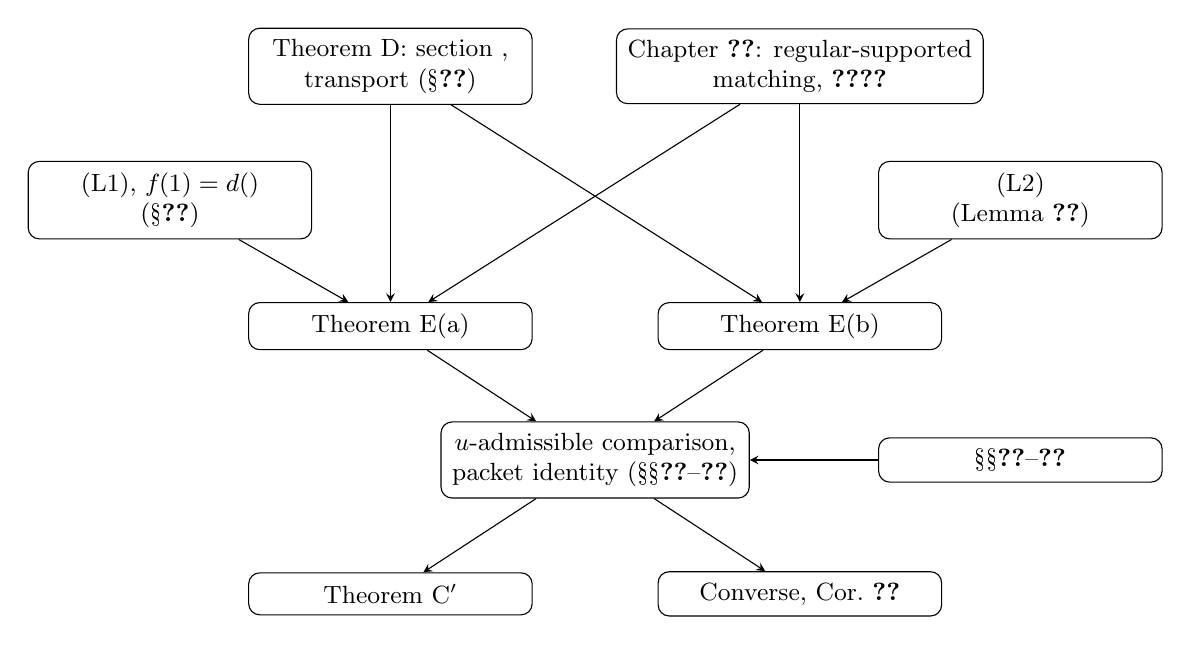
\begin{tikzpicture}[box/.style={draw,rounded corners,align=center,font=\small,inner sep=4pt,minimum width=3.6cm},>=stealth]
\node[box] (D) at (-2.6,0) {Theorem D: section $\sg$,\\ transport (\S\ref{II:sec:center})};
\node[box] (B) at (2.6,0) {Chapter~\ref{ch:I}: regular-supported\\ matching, \cref{I:lem:transported,I:lem:Aprops}};
\node[box] (L1) at (-5.4,-1.7) {(L1), $f_{\St}(1)=d(\St)$\\ (\S\ref{II:subsec:linear})};
\node[box] (L2) at (5.4,-1.7) {(L2)\\ (Lemma~\ref{II:lem:L2})};
\node[box] (Ea) at (-2.6,-3.3) {Theorem E(a)};
\node[box] (Eb) at (2.6,-3.3) {Theorem E(b)};
\node[box] (P) at (0,-5.0) {$u$-admissible comparison,\\ packet identity (\S\S\ref{II:subsec:uadm}--\ref{II:subsec:packet2})};
\node[box] (PI) at (5.4,-5.0) {\S\S\ref{I:sec:global}--\ref{I:sec:spectral}};
\node[box] (C) at (-2.6,-6.7) {Theorem C$'$};
\node[box] (Cc) at (2.6,-6.7) {Converse, Cor.~\ref{II:cor:Hprimesq}};
\draw[->] (D)--(Ea); \draw[->] (D)--(Eb); \draw[->] (B)--(Ea); \draw[->] (B)--(Eb);
\draw[->] (L1)--(Ea); \draw[->] (L2)--(Eb);
\draw[->] (Ea)--(P); \draw[->] (Eb)--(P); \draw[->] (PI)--(P); \draw[->] (P)--(C); \draw[->] (P)--(Cc);
\end{tikzpicture}
\end{center}
The germ results (Corollary~\ref{II:cor:germexp}, Lemma~\ref{II:lem:cuspnear1}, Corollary~\ref{II:cor:trivgerm}, Theorem~\ref{II:thm:germ}(b)) and the cancellation criterion (Proposition~\ref{II:prop:cancel2}) are not used in the proofs of Theorems~D, E and C$'$.

\subsection{Conventions and labels}\label{II:subsec:labels}
We keep the conventions and the labeling scheme of Chapter~\ref{ch:I}. They are collected, with the rest of the series' notation and the cocycle normalization, in the shared glossary of \S\ref{II:sec:glossary} (labels in \S\ref{gl:labels}, covers and the relabeling of $\mu_n$ in \S\ref{gl:cocycle}, Haar measures in \S\ref{gl:measures}).

All Hilbert symbols are $n$-th Hilbert symbols, and $\mu_n$ is relabeled once by $\zeta\mapsto\zeta^{r'}$ as in \S\ref{I:subsec:conventions}. Statements are marked by status, with proved-here the default and carrying no visible tag:

\emph{Proved here} (no tag): a complete argument is included, possibly using results marked \Ev. For global statements, ``proved'' means proved relative to the cited results of Chapter~\ref{ch:I}, which are restated in \S\ref{II:subsec:fromPartI}.
\begin{itemize}
\item \Ev\ \emph{Established elsewhere}: a precisely cited theorem, used as a black box. Several of these are results of Kazhdan \cite{Kaz86} that Flicker and Kazhdan state for covers in \cite{FK86}; we cite them in the form stated in \cite{FK86}.
\item \Ov\ \emph{Proof outlined}: the steps are identified, but at least one remains to be written out or checked.
\item \Cv\ \emph{Conjectural}: requires new mathematical input (later parts of the series).
\end{itemize}
A remark immediately after each \Ev, \Ov\ or \Cv\ statement explains its status.

\begin{center}
\begin{tabular}{>{\raggedright\arraybackslash}p{0.55\textwidth}>{\raggedright\arraybackslash}p{0.16\textwidth}>{\raggedright\arraybackslash}p{0.2\textwidth}}
\toprule
Statement & Where & Status\\
\midrule
Compatible measures at $S$; Chapter~\ref{ch:I} unaffected & \S\ref{II:subsec:measures} & \Pv\\
$n$-th roots; the section $\sg$; compatibility with $\jj$ (Theorem~D) & \S\S\ref{II:subsec:roots}--\ref{II:subsec:section} & \Pv\\
Transport; regular elements near $\Zb_v$ are good (Theorem~D) & \S\ref{II:subsec:transport} & \Pv\\
Germ expansion at central good elements & Cor.~\ref{II:cor:germexp} & \Pv\ using \Ev\\
Orbital integrals of arbitrary genuine functions ($r$ prime) & \S\ref{II:sec:arbitrary} & \Pv\\
Linear inputs (L1), (L2), $f_{\St}(1)=d(\St)$ & \S\ref{II:subsec:linear} & \Pv\ using \Ev\\
The pair $(e_D,\tilde f^{\St})$ & Prop.~\ref{II:prop:eD} & \Pv\\
Matching of arbitrary functions (Theorem~E) & Thm.~\ref{II:thm:matching} & \Pv\\
Required germ near the center: orbital-integral form & Thm.~\ref{II:thm:germ}(a) & \Pv\\
Unipotent orbital integrals of functions cuspidal near $1$; the trivial germ & Lemma~\ref{II:lem:cuspnear1}, Cor.~\ref{II:cor:trivgerm} & \Pv\ using \Ev\\
Required germ: unipotent form (G1), (G2) & Thm.~\ref{II:thm:germ}(b) & \Pv\\
Comparison and packet identity with $u$-admissible pairs & \S\S\ref{II:subsec:uadm}--\ref{II:subsec:packet2} & \Pv\ relative to Chapter~\ref{ch:I}\\
Theorem~C$'$ and its converse & \S\ref{II:subsec:Cprime} & \Pv\ relative to Chapter~\ref{ch:I}, under $(\mathrm{Hyp}_D')$, $(\mathrm{Hyp}')$\\
Cancellation criterion for $(\mathrm{Hyp}_D')$; finitely many $S$-types suffice & Prop.~\ref{II:prop:cancel2}, Cor.~\ref{II:cor:finiteStypes} & \Pv\\
Local character relations; unconditional transfer & \S\ref{II:sec:partIII} & \Cv\ (character relations at tame places: Chapter~\ref{ch:III})\\
\bottomrule
\end{tabular}
\end{center}

\subsection*{The running example}
The series' running example is $K=\mathbb{Q}(\zeta_3)$, $n=3$, $r=2$, $D=(-1,4-\zeta_3)_K$, ramified exactly at $S=\{\mathfrak p_3,\mathfrak p_7\}$, with $\mathfrak p_3=(1-\zeta_3)$ and $\mathfrak p_7=(3+\zeta_3)$ (Example~\ref{ex:running}, and \cite{JRE26}). Definition~\ref{II:def:measures} fixes $\mathrm{vol}(D_v^\times/F^\times)=d(\St)^{-1}$ at both places of $S$. Theorem~E applies at both. At the wild place $\mathfrak p_3$, where the covered elliptic tori are non-abelian, matching near the center uses Theorem~D. In Theorem~C$'$ the place $u$ is $\mathfrak p_3$ or $\mathfrak p_7$, and $(\mathrm{Hyp}_D')$ is a condition on test functions at these two places.

\subsection{Organization}
Section~\ref{II:sec:recall} recalls what we use from Chapter~\ref{ch:I} and fixes the Haar measures at the ramified places. Sections~\ref{II:sec:center}--\ref{II:sec:matching} contain the local theory: the section $\sg$ and the transport (\S\ref{II:sec:center}), orbital integrals of arbitrary genuine functions away from the center (\S\ref{II:sec:arbitrary}), and matching of arbitrary functions (\S\ref{II:sec:matching}). Section~\ref{II:sec:CC} proves Theorem~C$'$. Section~\ref{II:sec:partIII} lists what is left for Chapter~\ref{ch:III}. Section~\ref{II:sec:glossary} collects the notation of the series and the notation specific to Chapter~\ref{ch:II}, and Section~\ref{II:sec:lit} discusses the work related to this Part; the literature of the whole series is reviewed in \S\ref{I:sec:lit}.

% =====================================================================
\section{Recollections from Chapter~\ref{ch:I}, and Haar measures}\label{II:sec:recall}
This section recalls the notation of Chapter~\ref{ch:I} that is used throughout, and fixes the Haar measures at the ramified places once and for all. It depends only on Chapter~\ref{ch:I}, whose results used here are restated in \S\ref{II:subsec:fromPartI} as (I1)--(I11). It introduces the local notation $P_g$, $A_g$, $\Phi^z$, the compatible measures of Definition~\ref{II:def:measures}, and the constant $\lambda_v$.

\subsection{Local notation}\label{II:subsec:localnotation}
We fix the local notation used in \S\S\ref{II:sec:center}--\ref{II:sec:matching}.

Throughout \S\S\ref{II:sec:center}--\ref{II:sec:matching}, $v$ is a finite place, $F=K_v$, $\fp$ its maximal ideal, $\varpi$ a uniformizer and $p$ the residual characteristic. We write $G$ for either $\GL(r,F)$ (embedded in $\cG_v$ by $\iG$) or $D_v^\times$ (embedded by $\iD$), $\Gb=p^{-1}(G)\subset\cGb_v$, $Z=F^\times$ and $\Zb=p^{-1}(Z)$, which is central and common to both covers (\cref{I:lem:center}). For $g\in G$ let $P_g$ be its characteristic polynomial (reduced characteristic polynomial if $G=D_v^\times$), $A_g:=F[g]$ the commutative $F$-algebra it generates, and call the roots of $P_g$ in $\ov F$ the eigenvalues of $g$. For a genuine character $\tilde\theta$ of $\Zb$, $C_c^\infty(\Gb,\tilde\theta)_\gen$ is the space of smooth genuine functions with $\tilde f(z\tilde g)=\tilde\theta(z)^{-1}\tilde f(\tilde g)$ and support compact modulo $\Zb$. Orbital integrals $\Phi$ and $F=\Delta\Phi$ are those of \cref{I:def:oi}, with $\Delta(\gamma)=|D(\gamma)|^{1/2}|\det\gamma|^{-(r-1)/2}$; as in \cite[\S6]{FK86}, $D(\gamma)$ is formed from the distinct eigenvalues. We also use the variant $\Phi^z(\gamma,f)=\int_{Z\backslash G}f(g^{-1}\gamma g)\,dg$ of \cite[\S6]{FK86} for regular elliptic $\gamma$; then $\Phi^z(\gamma,f)=\vol(T_\gamma/Z)\,\Phi(\gamma,f)$.

\subsection{Haar measures at the ramified places}\label{II:subsec:measures}
We fix compatible Haar measures at the places of $S$ (Definition~\ref{II:def:measures}), used in the rest of the chapter. This choice is made once and for all; it simplifies the normalization at the identity and the formal-degree relations of \S\ref{II:sec:partIII}(ii).

Measures are as in \S\ref{I:subsec:oi}: $dg$ on $G/Z$, $dt$ on $T/Z$, and $dg/dt$ on $T\backslash G$; at $v\in S$ they are specialized as follows.

\begin{definition}[Compatible measures]\label{II:def:measures}\index{compatible measures@Compatible measures}
At each $v\in S$, let $dg_v$ be any Haar measure on $\GL(r,F)/F^\times$, and let $d(\St)=d(\St;dg_v)$ be the formal degree, with respect to $dg_v$, of the Steinberg representation of $\GL(r,F)$ (trivial central character). Normalize the Haar measure $dg_{D,v}$ on the compact group $D_v^\times/F^\times$ by
\[ \vol(D_v^\times/F^\times;\,dg_{D,v})=d(\St;dg_v)^{-1}. \]
The measures $dt$ on tori are arbitrary, as in Chapter~\ref{ch:I} (matching does not depend on them).
\end{definition}

\begin{remark}\label{II:rem:measures}
(1) \S\ref{I:subsec:measures} allows arbitrary $dg_v$ and $dg_{D,v}$ at $v\in S$, provided matching and the trace formulas use the same ones. So every result of Chapter~\ref{ch:I}, local and global, holds with the measures of Definition~\ref{II:def:measures}, and we cite Chapter~\ref{ch:I} without change.

(2) The formal degree of the trivial representation of $D_v^\times$ is $\vol(D_v^\times/F^\times)^{-1}$, and the trivial representation corresponds to $\St$ under the linear Jacquet--Langlands correspondence \cite[Theorem~2.2]{Bad08}. So Definition~\ref{II:def:measures} says that this pair has equal formal degrees. We expect that it agrees with Kottwitz's normalization of measures on inner forms \cite{Kot88}, but nothing below uses this.

(3) For arbitrary measures, the constant $\lambda_v:=d(\St)\vol(D_v^\times/F^\times)$ would appear in the normalization at the identity (Theorem~\ref{II:thm:germ}(c)). Definition~\ref{II:def:measures} is exactly the condition $\lambda_v=1$.
\end{remark}

\subsection{Statements used from Chapter~\ref{ch:I}}\label{II:subsec:fromPartI}
For the reader's convenience, and to make the dependence on Chapter~\ref{ch:I} auditable, we restate the results of Chapter~\ref{ch:I} that are used, in the form used. Numbers refer to Chapter~\ref{ch:I}. The labels (I1)--(I11) are used in the rest of the paper.

\begin{enumerate}[label=(I\arabic*)]
\item \emph{Admissible functions} (\S\ref{I:subsec:transported}). For $\bullet\in\{D,\GL\}$ and an elliptic torus of type $i$, a function $h$ on the good regular elements $Z(\Eb_{i,\bullet})^{\reg}$ is admissible if it is (i) locally constant, (ii) satisfies $h(z\tilde t)=\tilde\theta_v(z)^{-1}h(\tilde t)$ for $z\in\Zb_v$, (iii) has support compact modulo $\Zb_v$ with closure contained in the regular set, and (iv) is invariant under the normalizer of the torus.
\item \emph{\Cref{I:lem:transported}.} (b) $h\mapsto h\circ\jj_i^{-1}$ is a bijection between admissible functions on the two sides. (c) Every admissible $h$ equals $F(\cdot,\tilde f_i)$ on $Z(\Eb_{i,\bullet})^{\reg}$ for some $\tilde f_i\in C_c^\infty$ supported on the good regular elements conjugate into that torus; $F(\tilde\delta,\tilde f_i)=0$ for regular $\tilde\delta$ not conjugate into it.
\item \emph{\Cref{I:thm:easy}.} (a) Every $\tilde f_D$ vanishing near $\Zb_v$ has a matching $\tilde f$ supported on the good regular elliptic set. (b) Every $\tilde f$ supported in the regular set with vanishing orbital integrals at good regular non-elliptic elements has a matching $\tilde f_D$ vanishing near $\Zb_v$.
\item \emph{\Cref{I:prop:germ}.} For $\tilde f_D$ there are a normal open compact $U\subset D_v^\times$ and a splitting $\kappa_U$ with $F(z\kappa_U(t),\tilde f_D)=\Delta(t)\vol(T\backslash D_v^\times)\tilde f_D(z)$ for $z\in\Zb_v$ and regular $t\in U$.
\item \emph{\Cref{I:lem:Asub}(b)} (Harish-Chandra). For $C\subset T^{\reg}$ and $\Omega\subset G$ compact modulo $Z$, the set of $\dot x\in T\backslash G$ with $x^{-1}Cx\cap\Omega\ne\emptyset$ is compact. (Stated in Chapter~\ref{ch:I} for any such $\Omega$.)
\item \emph{\Cref{I:lem:Aprops}.} For regular-supported $\tilde f$, $F(\cdot,\tilde f)$ on an elliptic torus is admissible. \emph{\Cref{I:lem:traceOI}.} Traces of regular-supported functions depend only on their good regular orbital integrals.
\item \emph{\Cref{I:prop:geomD}.} The $D$-side trace formula: $\sum m(\pib_D)\tr\pib_D(\tilde f_D)=\vol\cdot\tilde f_D(1)+\sum_{[\gamma]}c(\gamma)F(\iota(\gamma),\tilde f_D)$, the sum over rational regular classes modulo the center that are good everywhere; every non-central rational element of $G_D(K)$ is regular since $r$ is prime. No condition on the test function at $S$.
\item \emph{\Cref{I:prop:FKvariant}} (variant of \cite[\S18]{FK86}). For $\tilde f$ with (i) a supercusp form at some finite place $w_0$ and (ii) support in the regular elliptic set at some finite place $u$, and no condition elsewhere: $\sum_{\text{cuspidal}}m(\pib)\tr\pib(\tilde f)=\sum_{[\gamma]}c(\gamma)F(\iota(\gamma),\tilde f)$, the sum over rational regular elliptic classes good everywhere.
\item \emph{\Cref{I:thm:rational} and \cref{I:cor:rationalbij}.} If $\tilde f_{D,v}$ and $\tilde f_v$ match at every $v\in S$ (no support condition) and correspond via $\psi_v$ outside $S$, then $F(\iota(\gamma),\tilde f_D)=F(\iota(j\gamma),\tilde f)$, the local signs multiplying to $(-1)^{(r-1)|S|}=1$ (if $r$ is odd, $r-1$ is even; if $r=2$, $|S|$ is even because the local invariants of $D$ sum to $0$ and $K$ has no real places); and classes whose field does not embed in $D$ contribute $0$ whenever (M2) holds at all $v\in S$, since such a class is non-elliptic at some $v\in S$ (Albert--Brauer--Hasse--Noether).
\item \emph{\Cref{I:lem:nusep}.} For fixed levels at the finite places (with any test functions bi-invariant under them) and fixed $K_\infty$-types and infinitesimal character, only finitely many automorphic representations contribute on either side.
\item \emph{\Cref{I:lem:cancel} (proof).} For a level $U_v$ at $v\in S$ (split by $\kappa_v$, with $\tilde\theta_v\circ\kappa_v$ trivial on $U_v\cap K_v^\times$), the corner algebra satisfies $\mathcal H_v\cong\bigoplus_{\tau_v\in\mathcal T_v}\mathrm{End}(\tau_v^{U_v})$, and $\mathrm{ev}_{1,v}=\vol(\GDb(K_v)/\Zb_v)^{-1}\sum_{\tau_v}(\dim\tau_v)\tr\tau_v$ on $\mathcal H_v$; $\mathcal R_v=\ker\mathrm{ev}_{1,v}$.
\end{enumerate}

% =====================================================================
\section{Harmonic analysis near the center}\label{II:sec:center}
This section proves Theorem~D. We construct a canonical $n$-th root on a conjugation-invariant neighborhood of the unipotent set (\S\ref{II:subsec:roots}), lift it to an equivariant section $\sg$ of the cover (\S\ref{II:subsec:section}), and use $\sg$ to transport genuine functions supported near $\Zb$ to ordinary functions on $G/Z$, with the same orbital integrals (\S\ref{II:subsec:transport}). As a corollary, the germ expansion of genuine orbital integrals at central good elements is the Shalika germ expansion of the linear group (\S\ref{II:subsec:germexp}). Everything in this section holds at every finite place, including those above $n$, and on both covers. The section depends on \S\S\ref{I:sec:covers}--\ref{I:sec:tori} (the covers, scalar centrality and the identification $\jj$) and on the Shalika germ expansion for $\GL(r,F)$ \cite{Sha72}. It introduces the neighborhoods $V_M$, the constants $\delta_n$, $B$, $M_0$, $M_1$, the root $g^{1/n}$, the section $\sg$ and the transport $\mathcal T$.

\subsection{$n$-th roots near the unipotent set}\label{II:subsec:roots}
We define a canonical $n$-th root on a conjugation-invariant neighborhood of the unipotent set, and introduce $\Omega_M$, $V_M$, $\delta_n$, $B$, $M_0$ and $g^{1/n}$, which are used throughout. The point of using $n$-th roots is that the $n$-th power of a lift does not depend on the lift.

For $M\ge1$ let $\Omega_M$ be the set of monic polynomials of degree $r$ over $F$ that are congruent to $(X-1)^r$ coefficientwise modulo $\fp^M$, and put
\[ V_M:=\{g\in G:\ P_g\in\Omega_M\}. \]
\emph{Absolute values.} In this subsection $q=|\cO/\fp|$, $e=v_F(p)$ is the absolute ramification index, and $|x|_F=q^{-v_F(x)}$ is the normalized absolute value of $F$, extended uniquely to $\ov F$; on $\cO$-algebras we use the corresponding sup norm $\|\cdot\|$ on coordinates. (In terms of the $p$-adic absolute value $|\cdot|_p$ with $|p|_p=p^{-1}$, one has $|x|_F=|x|_p^{[F:\mathbb Q_p]}$.) Put
\[ \delta_n:=\begin{cases}1,&p\nmid n,\\ q^{-e/(p-1)},&p\mid n,\end{cases}\qquad B:=|n|_F^{-1}q^{e/(p-1)}. \]

\begin{lemma}\label{II:lem:roots}
\begin{enumerate}[label=(\alph*)]
\item $V_M$ is open, closed and stable under conjugation, and so is $ZV_M$. Every eigenvalue $\lambda$ of $g\in V_M$ satisfies $|\lambda-1|_F\le|\varpi|_F^{M/r}$.
\item If $u\in\ov F$, $u^n=1$ and $|u-1|_F<\delta_n$, then $u=1$.
\item $|\binom{1/n}{k}|_F\le B^k$ for all $k\ge0$. There is $M_0$ such that for $M\ge M_0$ and $g\in V_M$ the series $g^{1/n}:=\sum_{k\ge0}\binom{1/n}{k}(g-1)^k$ converges in $A_g$. Its sum is the unique $h\in A_g$ with $h^n=g$ whose eigenvalues $\mu$ satisfy $|\mu-1|_F<\delta_n$.
\item For $M\ge M_0$: $(xgx^{-1})^{1/n}=xg^{1/n}x^{-1}$ for $x\in G$; the map $g\mapsto g^{1/n}$ is continuous on $V_M$; and $(ag)^{1/n}=a^{1/n}g^{1/n}$ whenever $a\in F^\times$ and $a,g,ag\in V_{M_0}$.
\end{enumerate}
\end{lemma}
\begin{proof}
(a) The map $g\mapsto P_g$ is continuous and $\Omega_M$ is open and closed, so $V_M$ is open and closed; it is conjugation-stable because $P_g$ is. If $\mu=\lambda-1$, then $\mu$ is a root of $P_g(X+1)=X^r+\sum_{i<r}c_iX^i$ with $|c_i|_F\le|\varpi|_F^M$. If $|\mu|_F>1$, then $|\mu|_F^r\le|\varpi|_F^M|\mu|_F^{r-1}$ gives $|\mu|_F<1$, a contradiction; so $|\mu|_F\le1$ and $|\mu|_F^r\le|\varpi|_F^M$. For $ZV_M$: openness is clear. If $a_kg_k\to g$ with $g_k\in V_M$, then $\det g_k\in\cO^\times$ (its reduced norm, when $G=D_v^\times$), so $|a_k|_F^r\to|\det g|_F$ and the $a_k$ lie in a compact subset of $F^\times$; passing to a convergent subsequence $a_k\to a$, we get $g_k\to a^{-1}g\in V_M$, so $g\in ZV_M$.

(b) If $u\ne1$, then $u$ is a root of unity of order $m>1$ dividing $n$. If $p\nmid m$, the reduction of $u$ is a nontrivial root of unity in the residue field, so $|u-1|_F=1$. If $p\mid m$, some power $u^{m/p^a}$ is a primitive $p^a$-th root of unity $\zeta$ with $a\ge1$, and $|u-1|_F\ge|\zeta-1|_F\ge|\zeta_p-1|_F=|p|_F^{1/(p-1)}=q^{-e/(p-1)}$. (The first inequality holds because $u^j-1=(u-1)(u^{j-1}+\dots+1)$ with the second factor integral; the second because $|\zeta-1|_F=|p|_F^{1/(p^{a-1}(p-1))}$ for $\zeta$ of exact order $p^a$.)

(c) Since $\binom{1/n}{k}=n^{-k}\prod_{j<k}(1-jn)/k!$ and $v_p(k!)\le k/(p-1)$, we have $|\binom{1/n}{k}|_F\le|n|_F^{-k}|k!|_F^{-1}\le|n|_F^{-k}q^{ek/(p-1)}=B^k$. Put $y=g-1$. Since $P_g$ has integral coefficients, $y$ is integral over $\cO$, so $\cO[y]\subset A_g$ is a finitely generated, hence complete, $\cO$-module. By Cayley--Hamilton $y^r=-\sum_{i<r}c_iy^i\in\varpi^M\cO[y]$, so $y^{kr+i}\in\varpi^{kM}\cO[y]$. So the series converges in $\cO[y]$ as soon as $|\varpi|_F^MB^r<1$. Then $h^n=g$, by the identity $(\sum_k\binom{1/n}{k}X^k)^n=1+X$ in $\mathbb Q[[X]]$ and absolute convergence. Each $F$-algebra map $\chi:A_g\to\ov F$ is continuous, and $\chi(g)$ runs over the eigenvalues of $g$. Hence the eigenvalues of $h$ are the numbers $b(\lambda-1)$, where $b(x)=\sum_k\binom{1/n}{k}x^k$ and $|\lambda-1|_F\le|\varpi|_F^{M/r}$. Since $|b(x)-1|_F\le\max_{k\ge1}(B|x|_F)^k$, enlarging $M_0$ gives $|b(\lambda-1)-1|_F<\delta_n$. For uniqueness, if $h'$ is another such root, then $u:=h'h^{-1}\in A_g$ satisfies $u^n=1$, and each eigenvalue of $u$ is within $\delta_n$ of $1$ (ultrametric inequality, since the eigenvalues of $h$ are units). By (b) all eigenvalues of $u$ equal $1$. Since $X^n-1$ is separable, $u$ is semisimple, so $u=1$.

(d) Equivariance and multiplicativity follow from the uniqueness in (c): $xg^{1/n}x^{-1}\in A_{xgx^{-1}}$ is an $n$-th root of $xgx^{-1}$ with the right eigenvalues, and $a^{1/n}g^{1/n}\in A_g=A_{ag}$ is an $n$-th root of $ag$ whose eigenvalues are products of numbers within $\delta_n$ of $1$. For continuity, let $g_0\in V_M$. Suppose first that $G=\GL(r,F)$, or $G=D_v^\times$ with $D_v$ split, identified with $\GL(r,F)$ by some $D_v\cong M_r(F)$. Then $\Lambda:=\cO[g_0]\cO^r$ is a $g_0$-stable lattice (finitely generated since $g_0$ is integral), and $g_0^{-1}$ is also integral since $\det g_0\in\cO^\times$; so after conjugation $g_0\in\GL(r,\cO)$. On the open set $V_M\cap\GL(r,\cO)$ we have $y\in M_r(\cO)$ and $\|y^r\|\le|\varpi|_F^M$, so the series converges uniformly there. (Note that $V_M\not\subset\GL(r,\cO)$: for instance $\left(\begin{smallmatrix}1&\varpi^{-N}\\0&1\end{smallmatrix}\right)\in V_M$ for all $M,N$. This is why we conjugate.) If $D_v$ is a division algebra, then $V_M\subset\cO_D^\times$, since an element of $D_v$ with integral reduced characteristic polynomial lies in the maximal order $\cO_D$, and the same estimate holds in $\cO_D$. Conjugation is a homeomorphism, so continuity holds everywhere.
\end{proof}


\subsection{The section $\sg$}\label{II:subsec:section}
We now lift the $n$-th root to the cover, defining the section $\sg$ (and $\sg_D$, $\sg_{\GL}$) used in the rest of the chapter. The resulting section is equivariant, consists of good elements, and is compatible with every splitting in sight and with the identification $\jj$ of Chapter~\ref{ch:I}.

\begin{definition}[The section $\sg$]\index{section sg@Section $\sg$}
For $M\ge M_0$ and $g\in V_M$ put $\sg(g):=\tilde h^{\,n}$, where $h=g^{1/n}$ and $\tilde h$ is any lift of $h$ to $\Gb$. We write $\sg_D$ and $\sg_{\GL}$ when the group must be specified.
\end{definition}

Since two lifts of $h$ differ by $\zeta\in\mu_n$ and $\zeta^n=1$, $\sg(g)$ is well defined.

\begin{proposition}\label{II:prop:section}
Let $M\ge M_0$.
\begin{enumerate}[label=(\alph*)]
\item $\sg:V_M\to\Gb$ is a continuous section of $p$, and $\sg(xgx^{-1})=\tilde x\,\sg(g)\,\tilde x^{-1}$ for all $x\in G$ and any lift $\tilde x$.
\item For every $g\in V_M$, $\sg(g)$ commutes with $p^{-1}(\Cent_G(g))$. In particular, $\sg(\gamma)$ is good for every regular $\gamma\in V_M$, and $\sg(t)\in Z(\Tb)$ for every $t\in T\cap V_M$ and every maximal torus $T$.
\item If $a\in F^\times$ and $a,g,ag\in V_{M_0}$, then $\sg(a)\in\Zb$ and $\sg(ag)=\sg(a)\sg(g)$.
\item Let $W\subseteq V_{M_0}$ be an open compact subgroup over which $p$ splits by a homomorphism $\kappa$. Then there is an open compact subgroup $U\subseteq W\cap V_M$ with $u^{1/n}\in W$ for all $u\in U$, and $\sg|_U=\kappa|_U$. In particular, the splitting $\kappa_U$ of \cref{I:prop:germ}, is $\sg_D|_U$ (there $U=U_k$, $W=U_{k'}$, and $\kappa_U(t)=\kappa(s)^n$ with $s=t^{1/n}\in U_{k'}$).
\item If $u$ is unipotent and lies in the unipotent radical $N$ of a parabolic subgroup of $\GL(r,F)$, then $\sg(u)=s_N(u)$, where $s_N$ is the unique splitting of $p$ over $N$.
\item \emph{(Compatibility of the two sides.)} For $a\in F^\times\cap V_{M_0}$, $\sg_D(a)=\sg_{\GL}(a)$ in $\Zb$. Let $E\subset D_v$ be a maximal subfield, $j:E\hookrightarrow M_r(F)$ an embedding, and $\jj_{E,j}:Z(\Eb_D)\to Z(\Eb_{\GL})$ the canonical identification of \cref{I:thm:ident}. Then $\jj_{E,j}(z\,\sg_D(t))=z\,\sg_{\GL}(j(t))$ for $z\in\Zb$ and $t\in E^\times\cap V_M$.
\end{enumerate}
\end{proposition}
\begin{proof}
(a) Near any point, $g\mapsto g^{1/n}$ is continuous (Lemma~\ref{II:lem:roots}(d)) and $p$ has continuous local sections, so $\tilde h$ may be chosen to depend continuously on $g$ locally. Equivariance: $\tilde x\tilde h\tilde x^{-1}$ is a lift of $xhx^{-1}=(xgx^{-1})^{1/n}$, so $\tilde x\tilde h^n\tilde x^{-1}=(\tilde x\tilde h\tilde x^{-1})^n=\sg(xgx^{-1})$.

(b) If $c\in\Cent_G(g)$, then $c$ commutes with $A_g\ni h$, so for a lift $\tilde c$ we have $\tilde c\tilde h\tilde c^{-1}=\zeta\tilde h$ with $\zeta\in\mu_n$, and therefore $\tilde c\tilde h^n\tilde c^{-1}=\zeta^n\tilde h^n=\tilde h^n$.

(c) $a^{1/n}\in F^\times$, so its lifts lie in $\Zb$, which is central. Hence $\sg(ag)=(\widetilde{a^{1/n}}\,\tilde h)^n=\widetilde{a^{1/n}}^{\,n}\tilde h^n=\sg(a)\sg(g)$, using Lemma~\ref{II:lem:roots}(d).

(d) The root map $u\mapsto u^{1/n}$ is continuous at $1$ and fixes $1$, so some open compact subgroup $U\subseteq W\cap V_M$ satisfies $u^{1/n}\in W$ for $u\in U$. For such $u$, $\kappa(u^{1/n})$ is a lift of $u^{1/n}$, so $\sg(u)=\kappa(u^{1/n})^n=\kappa(u)$, since $\kappa$ is a homomorphism. We do \emph{not} assume $u^{1/n}\in U$: when $p\mid n$ this generally fails for the standard filtration subgroups, since a $p$-th root of an element of $1+\fp^m$ lies only in a larger principal-unit group.

(e) $u^{1/n}=\sum_k\binom{1/n}{k}(u-1)^k$ is a finite sum, and it lies in $N$. Since $s_N$ is a homomorphism, $\sg(u)=s_N(u^{1/n})^n=s_N(u)$.

(f) The first assertion holds because $\iD(a)=\iG(a)$ and $a^{1/n}\in F^\times$, so both sides are the $n$-th power of a lift of the same element of $\cG_v$. For the second, put $s=t^{1/n}\in F[t]\subseteq E$. Then $j(s)=j(t)^{1/n}$, by uniqueness in Lemma~\ref{II:lem:roots}(c), since $j$ is an $F$-algebra embedding and preserves eigenvalues. Let $\varphi\in\Iso_{\Zb}(\Eb_D,\Eb_{\GL})$. It is a group isomorphism over $\iG j\iD^{-1}$, so $\varphi(\sg_D(t))=\varphi(\tilde s)^n$, and $\varphi(\tilde s)$ is a lift of $j(s)$. Hence $\varphi(\sg_D(t))=\sg_{\GL}(j(t))$. By (b), $\sg_D(t)\in Z(\Eb_D)$, where $\varphi$ restricts to $\jj_{E,j}$; and $\varphi$ is the identity on $\Zb$.
\end{proof}

\begin{remark}
(1) Proposition~\ref{II:prop:section} holds equally for $v\mid n$; only $M_0$ grows. So the distinction between $v\mid n$ and $v\nmid n$, which governs the structure of the covered tori (\cref{I:prop:good}), plays no role near the center.

(2) Part~(e) says that $\sg$ extends the canonical lifting of unipotent elements. So the unipotent orbital integrals $\Phi(z\,\sg(u),\tilde f):=\int_{G_u\backslash G}\tilde f(\tilde x^{-1}z\sg(u)\tilde x)\,d\dot x$ are well defined by (b), and they are the unipotent orbital integrals of \cite[\S8]{FK86}, where unipotent elements are lifted by the splitting $s$ of \cite[\S2]{FK86} (see Remark~\ref{II:rem:FK8}(1) for the normalization of $F$).
\end{remark}


\subsection{Transport to the linear group}\label{II:subsec:transport}
We show that genuine functions supported in $p^{-1}(ZV_M)$ are the same thing as linear functions on $G/Z$ supported in $ZV_M$, with the same orbital integrals. This holds on both sides and is compatible with $\jj$. The constant $M_1$ and the transport $\mathcal T$ (and $\mathcal T_D$) defined here are used in \S\ref{II:sec:matching}.

\begin{lemma}[Choice of $M$]\label{II:lem:chooseM}
Let $\tilde\theta$ be a genuine character of $\Zb$. There is $M_1\ge M_0$ such that for $M\ge M_1$:
\begin{enumerate}[label=(\alph*)]
\item if $a\in F^\times$, $g\in V_M$ and $ag\in V_M$, then $a\in1+\fp^{\lceil M/r\rceil}\subseteq V_{M_0}$;
\item $\tilde\theta(\sg(a))=1$ for all $a\in1+\fp^{\lceil M/r\rceil}$.
\end{enumerate}
\end{lemma}
\begin{proof}
(a) If $\lambda$ is an eigenvalue of $g$, then $a\lambda$ is one of $ag$, and Lemma~\ref{II:lem:roots}(a) gives $|a-1|_F=|a\lambda-\lambda|_F/|\lambda|_F\le|\varpi|_F^{M/r}$. A scalar $a$ with $|a-1|_F\le|\varpi|_F^m$ has $P_a=(X-a)^r\in\Omega_m$. (b) By Proposition~\ref{II:prop:section}(c), $a\mapsto\tilde\theta(\sg(a))$ is a continuous character of $1+\fp^{M_0}$, so it is trivial on $1+\fp^m$ for $m$ large.
\end{proof}

\emph{Measure convention.} For $g\in G$ let $G_g$ be its centralizer. If $g\in V_M$, then $\sg(g)$ commutes with $p^{-1}(G_g)$ (Proposition~\ref{II:prop:section}(b)), so the genuine orbital integral $\Phi(z\sg(g),\tilde f)=\int\tilde f(\tilde x^{-1}z\sg(g)\tilde x)\,d\dot x$ is an integral over the same quotient space $G_g\backslash G$ as the linear orbital integral at $p(z)g$. Throughout, the two are computed with the \emph{same} quotient measure on $G_g\backslash G$: for regular $g$, the measure $dg/dt$ of \S\ref{I:subsec:oi}; for unipotent $g$, a fixed $G$-invariant measure on the class of $g$, used both in the Shalika expansion (Corollary~\ref{II:cor:germexp}) and in the Richardson formula of Lemma~\ref{II:lem:cuspnear1}. ``Same orbital integrals'' below always means equality for these measures.

Fix $M\ge M_1$, and let $C_c^\infty(\Gb,\tilde\theta)_{\gen,M}$ be the space of $\tilde f\in C_c^\infty(\Gb,\tilde\theta)_\gen$ supported in $p^{-1}(ZV_M)$, and $C_c^\infty(G/Z)_M$ the space of $\varphi\in C_c^\infty(G/Z)$ supported in $ZV_M$.

\begin{proposition}[Transport]\label{II:prop:transport}
\begin{enumerate}[label=(\alph*)]
\item Every element of $p^{-1}(ZV_M)$ is of the form $z\,\sg(g)$ with $z\in\Zb$ and $g\in V_M$. Every regular element of $p^{-1}(ZV_M)$ is good.
\item The formula $(\mathcal T\tilde f)(p(z)g):=\tilde\theta(z)\,\tilde f(z\,\sg(g))$ ($z\in\Zb$, $g\in V_M$) defines a linear bijection
\[ \mathcal T:C_c^\infty(\Gb,\tilde\theta)_{\gen,M}\xrightarrow{\ \sim\ }C_c^\infty(G/Z)_M, \]
with inverse $(\mathcal T^{-1}\varphi)(z\sg(g))=\tilde\theta(z)^{-1}\varphi(p(z)g)$ on $p^{-1}(ZV_M)$ and $0$ elsewhere.
\item For $z\in\Zb$ and regular $\gamma\in V_M$,
\[ \Phi(z\,\sg(\gamma),\tilde f)=\tilde\theta(z)^{-1}\,\Phi(p(z)\gamma,\mathcal T\tilde f),\qquad F(z\,\sg(\gamma),\tilde f)=\tilde\theta(z)^{-1}\,F(p(z)\gamma,\mathcal T\tilde f), \]
where on the right $\Phi$ and $F=\Delta\Phi$ are the linear orbital integrals with the same measures. More generally, the first identity holds for every $\gamma\in V_M$, with $\Phi$ the integral over $G_\gamma\backslash G$ (for instance, for unipotent $\gamma$).
\item For a function $\beta$ on $G$ that is constant on conjugacy classes and on $Z$-cosets, with $\beta\cdot1_{ZV_M}$ locally constant, $\mathcal T\big((\beta\circ p)\tilde f\big)=\beta\cdot\mathcal T\tilde f$.
\end{enumerate}
\end{proposition}
\begin{proof}
(a) If $\tilde x\in p^{-1}(ZV_M)$, write $p(\tilde x)=ag$ with $g\in V_M$, and choose a lift $z$ of $a$; then $\tilde x=\zeta z\sg(g)$ for some $\zeta\in\mu_n\subset\Zb$. A regular element $z\sg(\gamma)$ is good by Proposition~\ref{II:prop:section}(b), since $z$ is central.

(b) \emph{Independence of the lift $z$ of $a=p(z)$:} replacing $z$ by $\zeta z$ multiplies $\tilde\theta(z)$ by $\zeta$ and $\tilde f(z\sg(g))$ by $\zeta^{-1}$. \emph{Independence of the factorization:} if $ag=a'g'$ with $g,g'\in V_M$, then $g'=cg$ with $c=a/a'\in1+\fp^{\lceil M/r\rceil}$ (Lemma~\ref{II:lem:chooseM}(a)), so $\sg(g')=\sg(c)\sg(g)$ (Proposition~\ref{II:prop:section}(c)). With $z'$ a lift of $a'$, $z:=z'\sg(c)$ is a lift of $a$, and
\[ \tilde\theta(z')\tilde f(z'\sg(g'))=\tilde\theta(z')\tilde f(z\sg(g))=\tilde\theta(\sg(c))^{-1}\tilde\theta(z)\tilde f(z\sg(g))=\tilde\theta(z)\tilde f(z\sg(g)), \]
by Lemma~\ref{II:lem:chooseM}(b). So $\mathcal T\tilde f$ is a well-defined function on $ZV_M$, extended by $0$. It is $Z$-invariant by construction, locally constant because $\sg$ is continuous and $\tilde f$ is locally constant, and supported in the set $ZV_M$, which is open and closed (Lemma~\ref{II:lem:roots}(a)); its support is compact modulo $Z$ because that of $\tilde f$ is compact modulo $\Zb$. The inverse is well defined by the same computation, and it is smooth because $p^{-1}(ZV_M)$ is open and closed.

(c) For $x\in G$, $\tilde x^{-1}z\sg(\gamma)\tilde x=z\,\sg(x^{-1}\gamma x)$ by Proposition~\ref{II:prop:section}(a). Hence $\tilde f(\tilde x^{-1}z\sg(\gamma)\tilde x)=\tilde\theta(z)^{-1}(\mathcal T\tilde f)(x^{-1}p(z)\gamma x)$. Integrate over $T_\gamma\backslash G$, and note that $\Delta(p(z)\gamma)=\Delta(\gamma)$. For non-regular $\gamma\in V_M$ the same computation applies over $G_\gamma\backslash G$, since $\sg(\gamma)$ commutes with $p^{-1}(G_\gamma)$ (Proposition~\ref{II:prop:section}(b)).

(d) is immediate from the definitions.
\end{proof}


\subsection{The germ expansion at central good elements}\label{II:subsec:germexp}
We record what the transport says about germs. This is not needed for the matching theorem, but it identifies the germs of \cite[\S8]{FK86} and \cite[\S1]{KP86} at central elements.

\begin{corollary}[Germ expansion at central good elements]\label{II:cor:germexp}\ (using \Ev)
Let $\tilde f\in C_c^\infty(\Gb,\tilde\theta)_\gen$ with $G=\GL(r,F)$, and let $z\in\Zb$. There is a neighborhood $V'$ of $1$ such that for regular $\gamma\in V'$,
\[ \Phi(z\,\sg(\gamma),\tilde f)=\sum_{\mathcal O}\Gamma_{\mathcal O}(\gamma)\,\Phi(z\,\sg(u_{\mathcal O}),\tilde f), \]
where $\mathcal O$ runs over the unipotent conjugacy classes of $\GL(r,F)$ (partitions of $r$), $u_{\mathcal O}\in\mathcal O$, and the $\Gamma_{\mathcal O}$ are the Shalika germs of $\GL(r,F)$ for the measures fixed above. On the $D$ side the only unipotent class is $\{1\}$, and the expansion is \cref{I:prop:germ}.
\end{corollary}
\begin{proof}
Apply Proposition~\ref{II:prop:transport} to $\tilde f\cdot1_{p^{-1}(ZV_M)}$, and the Shalika germ expansion \cite{Sha72}, \cite{HC70} \Ev\ to $\mathcal T(\tilde f\cdot1_{p^{-1}(ZV_M)})$ at $1$. Since that function is $Z$-invariant, its expansion at $p(z)$ is its expansion at $1$. By Proposition~\ref{II:prop:transport}(c), applied also to the unipotent orbits, the factors $\tilde\theta(z)^{\pm1}$ cancel.
\end{proof}



\begin{remark}\label{II:rem:FK8}
(1) \cite[\S8, Theorem]{FK86} and \cite[Theorem~1.4]{KP86} (credited there to Shalika, Harish-Chandra, Vign\'eras and Kazhdan--Patterson) give a germ expansion of genuine orbital integrals at every semisimple element, with germs indexed by the good elements above it, and a converse characterizing orbital-integral functions \cite[Theorem~1.7]{KP86}. The germs are shown to exist; their structure is not determined there (\cite[\S1, Remark~2]{KP86}). Corollary~\ref{II:cor:germexp} identifies them, at central good elements, with the Shalika germs of $\GL(r,F)$. In comparing normalizations, note that \cite{FK86} normalize $F=\Delta\Phi$ with $\Delta$ formed from distinct eigenvalues, so that at $z\,\sg(u)$ with $z$ central $F=|\det z|^{-(r-1)/2}\Phi$.

(2) The principle that orbital integrals on covers near a semisimple element reduce to the Lie algebra of its centralizer is part of W.-W.~Li's semisimple descent \cite[\S4]{Li12}, and we make no claim of priority for Corollary~\ref{II:cor:germexp}. What we use is the explicit transport of Proposition~\ref{II:prop:transport}, which is compatible with \emph{both} covers and with $\jj$ (Proposition~\ref{II:prop:section}(f)).
\end{remark}

% =====================================================================
\section{Orbital integrals of arbitrary genuine functions}\label{II:sec:arbitrary}
This section extends the facts about orbital integrals on elliptic tori in \S\ref{I:app:oi}, from regular-supported functions to arbitrary genuine functions. For $r$ prime, the only singular elements near which the elliptic regular set accumulates are central (Lemma~\ref{II:lem:singular}), so once the behavior near $\Zb$ is removed, the elliptic orbital integrals of an arbitrary genuine function are admissible in the sense of \S\ref{I:subsec:transported} (Lemma~\ref{II:lem:Aext}). The section depends on \S\ref{I:app:oi}, and introduces no new notation.

\begin{lemma}[Singular elements, $r$ prime]\label{II:lem:singular}
Let $G=\GL(r,F)$ with $r$ prime. A non-central singular semisimple element $s$ has a neighborhood containing no regular elliptic element. Hence, for every elliptic maximal torus $T$, every point of $T\smallsetminus Z$ is regular, and $(T\smallsetminus ZV_M)/Z$ is a compact subset of $T^{\reg}/Z$.
\end{lemma}
\begin{proof}
Write $P_s=\prod_iQ_i^{m_i}$ with distinct monic irreducible $Q_i$. If there were only one factor, $P_s=Q^m$ with $m\deg Q=r$, so $m=1$ (then $P_s$ is separable and $s$ is regular) or $m=r$ and $\deg Q=1$ (then the semisimple element $s$ has a single eigenvalue in $F$ and is central). Both are excluded, so $P_s=AB$ with $A,B$ coprime and of positive degree. By Hensel's lemma, every monic polynomial close enough to $P_s$ factors as $A'B'$ with $\deg A'=\deg A$ and $\deg B'=\deg B$. So elements close to $s$ have reducible characteristic polynomials and are not elliptic. The second statement holds because the singular elements of $T$ are central, $T/Z$ is compact, and $T\smallsetminus ZV_M$ is closed.
\end{proof}

\begin{lemma}[Extension of \cref{I:lem:Aprops}]\label{II:lem:Aext}\ (using \Ev)
Let $\tilde f\in C_c^\infty(\Gb,\tilde\theta)_\gen$ be arbitrary, $T$ an elliptic maximal torus, and $h=F(\cdot,\tilde f)$ on $\Tb^{g,\reg}$. Then $h$ satisfies conditions (i), (ii) and (iv) of \S\ref{I:subsec:transported}. If moreover $h=0$ on $p^{-1}(ZV_M)\cap\Tb^{g,\reg}$ for some $M$, then $h$ is admissible.
\end{lemma}
\begin{proof}
The proofs of (ii) and (iv) in \cref{I:lem:Aprops}, do not use the support of $\tilde f$. The proof of (i) uses \cref{I:lem:Asub}(b), with $\Omega=p(\supp\tilde f)$; that lemma holds for every $\Omega$ compact modulo $Z$ \cite{HC70} \Ev. For (iii): $\supp h$ is closed in the open and closed subgroup $Z(\Tb)$ and contained in $p^{-1}(T\smallsetminus ZV_M)$, whose image in $T/Z$ is compact and regular by Lemma~\ref{II:lem:singular}.
\end{proof}



\begin{remark}
Lemma~\ref{II:lem:singular} is the only place where primality of $r$ enters the local theory of this chapter (besides its use in Chapter~\ref{ch:I}). For composite $r$ there are non-central singular semisimple elements with elliptic centralizers, of the form $\GL(m,E')$ with $m[E':F]=r$ and $m>1$. Germ expansions there exist by \cite[\S8]{FK86}, but they are not explicit, and the method of \S\ref{II:sec:center} would have to be extended to covers of $\GL(m,E')$.
\end{remark}

% =====================================================================
\section{Matching of arbitrary functions}\label{II:sec:matching}
This section proves Theorem~E. We first collect the inputs about the linear groups (\S\ref{II:subsec:linear}). We then construct the genuine analog of the pair (constant function on $D_v^\times$, Steinberg pseudo-coefficient on $\GL(r,F)$) near the center (\S\ref{II:subsec:steinberg}), prove matching in both directions (\S\ref{II:subsec:matchthm}), and determine the germ near the center that every matching function must have (\S\ref{II:subsec:germ}). Throughout, $v\in S$, $F=K_v$, and $\tilde\theta_v$ is a genuine character of $\Zb_v$, common to both covers. The section depends on \S\S\ref{II:sec:center}--\ref{II:sec:arbitrary}, on \S\ref{I:sec:matching}, and on the linear results of \cite{FK86}, \cite{Kaz86} and \cite{Bad08} cited in \S\ref{II:subsec:linear}. It introduces the linear inputs (L1), (L2), the functions $f_{\St}$, $e_D$, $\tilde f^{\St}$, and the conditions (Ell), (Non), (G1), (G2).

\subsection{Inputs about the linear groups}\label{II:subsec:linear}
We state the two linear inputs (L1) and (L2), which are used throughout this section, prove the value of the Steinberg pseudo-coefficient at the identity, and derive (L2) from statements in \cite{FK86} and \cite{Bad08}.

Let $G=\GL(r,F)$.
\begin{enumerate}[label=(L\arabic*)]
\item \Ev\ There is $f_{\St}\in C_c^\infty(G/Z)$, a pseudo-coefficient of the Steinberg representation, with $\tr\St(f_{\St})=1$, $\tr\pi'(f_{\St})=0$ for every irreducible tempered $\pi'\not\cong\St$ with trivial central character, $\Phi(\gamma,f_{\St})=(-1)^{r-1}\vol(T_\gamma/Z)^{-1}$ for regular elliptic $\gamma$, and $\Phi(\gamma,f_{\St})=0$ for regular non-elliptic $\gamma$.
\item (Lemma~\ref{II:lem:L2}) Every $\varphi\in C_c^\infty(G/Z)$ with $\Phi(\gamma,\varphi)=0$ for all regular non-elliptic $\gamma$ has a matching $\varphi_D\in C_c^\infty(D_v^\times/Z)$.
\end{enumerate}

\emph{Source of (L1).} \cite[\S25.1, Theorem]{FK86}, from \cite[Theorem~K]{Kaz86}, is stated for every square-integrable representation of the cover, and so, with $n=1$ (the convention of \cite[\S8, Remark~(3)]{FK86}), for $\GL(r,F)$. It gives $\Phi^z(\gamma,f_{\St})=\ov{\Theta_{\St}(\gamma)}$ on the regular elliptic set and $\Phi^z=0$ at regular non-elliptic elements, together with the trace properties. Since $\Phi^z=\vol(T_\gamma/Z)\Phi$ and $\Theta_{\St}=(-1)^{r-1}$ on the regular elliptic set, this is (L1). The value of $\Theta_{\St}$ follows from \cite[Theorem~2.2]{Bad08} with $n=1$, $d=r$, since the trivial representation of $D_v^\times$ corresponds to $\St$.

\begin{remark}\label{II:rem:centralchar}
\emph{From compact support to trivial central character.} The linear statements (L1), (L2) are usually formulated for $C_c^\infty(G)$ with measures on $G$ and $T$. Choose $b\in C_c^\infty(F^\times)$ supported in small neighborhoods of representatives of $F^\times/F^{\times r}$ (a finite group), normalized so that $\int_{F^\times}b(z^ry)\,dz=1$ for all $y$. For $\varphi\in C_c^\infty(G/Z)$, the function $\varphi':=\varphi\cdot(b\circ\det)$ (respectively $b\circ\Nrd$) lies in $C_c^\infty(G)$, satisfies $\int_Z\varphi'(zg)\,dz=\varphi(g)$, and has orbital integrals $b(\det\gamma)$ times those of $\varphi$. In particular $\varphi'$ is cuspidal if $\varphi$ is. Since averaging over $Z$ commutes with matching ($z\gamma\leftrightarrow z\gamma'$, $\Delta(z\gamma)=\Delta(\gamma)$), matching statements for $C_c^\infty$ imply the same statements for $C_c^\infty(\cdot/Z)$.
\end{remark}
\begin{lemma}[Value of $f_{\St}$ at the identity]\label{II:lem:fSt1}\ (using \Ev)
With $f_{\St}$ as in (L1), $f_{\St}(1)=d(\St)$, the formal degree of $\St$ with respect to $dg$.
\end{lemma}
\begin{proof}
By Harish-Chandra's Plancherel formula for $G/Z$ with trivial central character \cite[Th\'eor\`eme~VIII.1.1, in the form (3) of \S VIII.1]{Wal03} (in explicit form for $\GL(n)$, see \cite{AP05}), for $f\in C_c^\infty(G/Z)$,
\[ f(1)=\sum_{\pi}d(\pi)\tr\pi(f)+\sum_{P\ne G}\int\tr\big(\mathrm{Ind}_P^G\sigma\big)(f)\,d\mu_P(\sigma), \]
where $\pi$ runs over square-integrable representations with trivial central character, and the second sum runs over proper standard parabolic subgroups $P=MN$, with $\sigma$ running over unitary twists of square-integrable representations of $M$ and $\mu_P$ absolutely continuous Plancherel measures. For $\GL(r,F)$ every $\mathrm{Ind}_P^G\sigma$ here is irreducible and tempered (the segments attached to unitary twists of square-integrable representations are pairwise unlinked, so \cite[Theorem~9.7(a)]{Zel80} applies), and it is not square-integrable when $P\ne G$, so it is not $\St$. By \cite[\S25.1, Theorem]{FK86} with $n=1$, $\tr\pi'(f_{\St})=0$ for every irreducible tempered $\pi'\not\cong\St$, and $\tr\St(f_{\St})=1$. Hence only the term $\pi=\St$ survives, and $f_{\St}(1)=d(\St)$.
\end{proof}




\begin{lemma}[The linear input (L2)]\label{II:lem:L2}\ (using \Ev)
Let $G=\GL(r,F)$, $r$ prime, and let $\varphi\in C_c^\infty(G/Z)$ satisfy $\Phi(\gamma,\varphi)=0$ for all regular non-elliptic $\gamma$. Then there is $\varphi_D\in C_c^\infty(D_v^\times/Z)$ with $F(t,\varphi_D)=(-1)^{r-1}F(j(t),\varphi)$ for every regular $t\in D_v^\times$ and every embedding $j$ of $F[t]$ in $M_r(F)$.
\end{lemma}
\begin{proof}
\emph{Step 1 (finitely many discrete series).} Let $\varphi$ be bi-invariant under an open compact subgroup $K'$. Then $\tr\pi(\varphi)\ne0$ only if $\pi^{K'}\ne0$. There are only finitely many square-integrable $\pi$ with trivial central character and $\pi^{K'}\ne0$: by Harish-Chandra's finiteness theorem \cite[Th\'eor\`eme~VIII.1.2]{Wal03} \Ev\ these form finitely many orbits under twisting by unramified characters $|\det|^s$, and in each orbit only finitely many members have trivial central character (the twist multiplies the central character by $|z|^{rs}$). Let $\Pi$ be this finite set, and for $\pi\in\Pi$ let $f_\pi$ be a pseudo-coefficient as in \cite[\S25.1, Theorem]{FK86} with $n=1$ \Ev. Put
\[ \psi:=\varphi-\sum_{\pi\in\Pi}\tr\pi(\varphi)\,f_\pi . \]

\emph{Step 2 ($\psi$ has vanishing tempered traces).} Let $\pi'$ be irreducible and tempered, with trivial central character. If $\pi'$ is square-integrable, then $\tr\pi'(\psi)=\tr\pi'(\varphi)-\tr\pi'(\varphi)=0$ by the defining property of the $f_\pi$ (and $\tr\pi'(\varphi)=0$ if $\pi'\notin\Pi$). Otherwise $\pi'=\mathrm{Ind}_P^G\sigma$ with $P\ne G$ and $\sigma$ a unitary twist of a square-integrable representation of $M$ (the classification of tempered representations of $\GL(r,F)$; \cite[\S9]{Zel80}), and $\tr\pi'(f_\pi)=0$ by \cite[\S25.1]{FK86}. Also $\tr\pi'(\varphi)=0$: by the Weyl integration formula (characters are locally integrable \cite[\S13]{FK86}), $\tr\pi'(\varphi)$ is a sum over conjugacy classes of maximal tori of integrals of $\Theta_{\pi'}\cdot\Phi(\cdot,\varphi)$. On non-elliptic tori $\Phi(\cdot,\varphi)=0$ by hypothesis, and on elliptic tori $\Theta_{\pi'}=0$, since the character of a representation induced from a proper parabolic subgroup vanishes on the regular elliptic set \cite{vD72} \Ev.

\emph{Step 3 (density).} We use \cite[\S27.3, Proposition]{FK86} \Ev\ with $n=1$. For $n=1$ the cover is $G$ itself, $x^*=x$, every representation is genuine and relevant, and the correspondence of \cite[\S26]{FK86} is the identity (the character relation (26.1) becomes $\Theta_{\tilde\pi}=\Theta_\pi$); ``matching'' means equality of $F(x,\cdot)$ at regular $x$. The proposition then reads: \emph{if $f,f'\in C_c^\infty(G/Z)$ satisfy $\tr\pi(f)=\tr\pi(f')$ for every irreducible tempered $\pi$ with trivial central character, then $F(x,f)=F(x,f')$ for every regular $x$.} Apply it with $f=\psi$ and $f'=0$, using Step~2. (For covers in general, the corresponding density of tempered characters is proved in \cite{Li12}.) So $\Phi(\gamma,\varphi)=\sum_{\pi\in\Pi}\tr\pi(\varphi)\Phi(\gamma,f_\pi)$ for all regular $\gamma$, and on the regular elliptic set
\[ \Phi^z(\gamma,\varphi)=\sum_{\pi\in\Pi}c_\pi\ov{\Theta_\pi(\gamma)},\qquad c_\pi:=\tr\pi(\varphi). \]

\emph{Step 4 (transfer).} By \cite[Theorem~2.2]{Bad08} with $n=1$, $d=r$ \Ev, there is a bijection $\pi\mapsto C(\pi)$ from essentially square-integrable representations of $\GL(r,F)$ to irreducible representations of $D_v^\times$, preserving central characters, with $\Theta_{C(\pi)}(t)=(-1)^{r-1}\Theta_\pi(j(t))$ for regular $t$. For an irreducible representation $\tau$ of $D_v^\times$ with trivial central character, put $f_\tau:=\vol(D_v^\times/Z)^{-1}\,\ov{\Theta_\tau}\in C_c^\infty(D_v^\times/Z)$. Since $f_\tau$ is conjugation invariant, $\Phi^z(t,f_\tau)=\vol(D_v^\times/Z)f_\tau(t)=\ov{\Theta_\tau(t)}$. Put $\varphi_D:=\sum_{\pi\in\Pi}c_\pi f_{C(\pi)}$. Then
\[ \Phi^z(t,\varphi_D)=\sum_\pi c_\pi\ov{\Theta_{C(\pi)}(t)}=(-1)^{r-1}\sum_\pi c_\pi\ov{\Theta_\pi(j(t))}=(-1)^{r-1}\Phi^z(j(t),\varphi). \]
Divide by $\vol(T/Z)$, which is the same on both sides because the same $dt$ is used on $T$ and $j(T)$ (\S\ref{I:subsec:oi}), and multiply by $\Delta(t)=\Delta(j(t))$. The measure $dg_{D,v}$ enters only through $\vol(D_v^\times/Z)$ in $f_\tau$ and in $\Phi^z(t,\cdot)$, and cancels.

\emph{On the complex conjugate.} The identity $\Phi^z(\gamma,f_\pi)=\ov{\Theta_\pi(\gamma)}$ is the normalization compatible with $\tr\pi(f_\pi)=1$: by the Weyl integration formula, for $f$ with vanishing non-elliptic orbital integrals, $\tr\pi'(f)=\sum_T(|W_T|\vol(T/Z))^{-1}\int_{T/Z}\Delta(t)^2\Theta_{\pi'}(t)\Phi^z(t,f)\,dt$, which for $\Phi^z(\cdot,f)=\ov{\Theta_\pi}$ is the elliptic inner product $\langle\Theta_{\pi'},\Theta_\pi\rangle$ of \cite[\S24]{FK86}, equal to $\delta_{\pi\pi'}$ for square-integrable $\pi'$ \cite[\S25]{FK86}. In any case the argument is insensitive to this convention: replacing $\ov{\Theta}$ by $\Theta$ throughout Steps~3 and~4 changes nothing, because the transfer identity of Step~4 has real coefficients $(-1)^{r-1}$.
\end{proof}

\begin{remark}
Lemma~\ref{II:lem:L2}, combined with Remark~\ref{II:rem:centralchar}, is the converse half of the linear transfer of functions of \cite{DKV84}. We include the proof because \cite[\S4.6]{Bad08} states only the regular-supported case, and because it uses only results whose statements we have checked in \cite{FK86} and \cite{Bad08}.
\end{remark}


\subsection{The Steinberg-type function}\label{II:subsec:steinberg}
We construct the genuine analog, near the center, of the pair (constant function on $D_v^\times$, Steinberg pseudo-coefficient). It exists as a pair of functions with matching orbital integrals; it is not a pair of pseudo-coefficients of single genuine representations. The functions $e_D$ and $\tilde f^{\St}$ defined here enter Theorem~E.

Fix $M\ge M_1$ (for $\tilde\theta_v$, on both sides) and put
\begin{gather*} e_D:=\mathcal T_D^{-1}\big(1_{ZV_{D,M}}\big)\in C_c^\infty(\GDb(K_v),\tilde\theta_v)_\gen,\\ \tilde f^{\St}:=d(\St)^{-1}\,\mathcal T^{-1}\big(f_{\St}\cdot1_{ZV_M}\big)\in C_c^\infty(\Gb_v,\tilde\theta_v)_\gen, \end{gather*}
with $f_{\St}$ as in (L1). Here $1_{ZV_{D,M}}\in C_c^\infty(D_v^\times/Z)$ because $D_v^\times/Z$ is compact and $ZV_{D,M}$ is open and closed. Concretely, $e_D(z\sg_D(g))=\tilde\theta_v(z)^{-1}$ for $g\in V_{D,M}$, and $e_D=0$ off $p^{-1}(ZV_{D,M})$. So $e_D(1)=1$.

\begin{proposition}\label{II:prop:eD}\ (using (L1))
The functions $e_D$ and $\tilde f^{\St}$ match. Explicitly, $\tilde f^{\St}(1)=1=e_D(1)$, and at good regular elements
\[ F(z\sg(\gamma),\tilde f^{\St})=\begin{cases}(-1)^{r-1}\tilde\theta_v(z)^{-1}\Delta(\gamma)\big(d(\St)\vol(T_\gamma/Z)\big)^{-1}&\gamma\in V_M\text{ regular elliptic},\\ 0&\gamma\in V_M\text{ regular non-elliptic},\end{cases} \]
and $F(\cdot,\tilde f^{\St})=0$ at good regular elements outside $p^{-1}(ZV_M)$.
\end{proposition}
\begin{proof}
By Proposition~\ref{II:prop:transport}(c),(d), $F(z\sg(\gamma),\tilde f^{\St})=d(\St)^{-1}\tilde\theta_v(z)^{-1}1_{V_M}(\gamma)\Delta(\gamma)\Phi(\gamma,f_{\St})$, and (L1) gives the displayed values. On the $D$ side, $e_D(\tilde x^{-1}z\sg_D(t)\tilde x)=\tilde\theta_v(z)^{-1}1_{V_{D,M}}(t)$, so $F(z\sg_D(t),e_D)=\tilde\theta_v(z)^{-1}1_{V_{D,M}}(t)\Delta(t)\vol(D_v^\times/Z)/\vol(T/Z)$, and $\vol(D_v^\times/Z)=d(\St)^{-1}$ by Definition~\ref{II:def:measures}. Outside $p^{-1}(ZV_{D,M})$ and $p^{-1}(ZV_M)$ both orbital integrals vanish, and $\jj$ preserves these sets, since it preserves characteristic polynomials and is the identity on $\Zb_v$. Now compare, using Proposition~\ref{II:prop:section}(f), the equality $1_{V_{D,M}}(t)=1_{V_M}(j(t))$, and the sign $(-1)^{r-1}$ in (M1).
\end{proof}

\begin{remark}[Not a pseudo-coefficient of one genuine representation]\label{II:rem:notpc}
$\tilde f^{\St}$ is defined by orbital integrals, not by representations, and matching needs nothing more. Under the character relations (D2) of Chapter~\ref{ch:I} (proved at tame places where the corrected Flicker--Kazhdan correspondence is available, for example when $(n,N_r)=1$; see \S\ref{II:sec:partIII}(ii)), $\tr\pib(\tilde f^{\St})=\tr\pib_D(e_D)$ for corresponding pairs. Now $\tr\tau(e_D)=\int_{\GDb(K_v)/\Zb_v}e_D\,\Theta_\tau$, which is the integral of $g\mapsto\Theta_\tau(\sg_D(g))$ over $ZV_{D,M}/Z$, is in general nonzero for more than one genuine irreducible $\tau$ (Fourier inversion on the compact group $\GDb(K_v)/\Zb_v$ expresses $e_D$ in terms of the characters of all $\tau$ of level contained in $V_{D,M}$). So $\tilde f^{\St}$ should be a combination of pseudo-coefficients of several genuine square-integrable representations, not the pseudo-coefficient of a single ``genuine Steinberg'' representation. Accordingly, the phrase ``a genuine analog of a Steinberg pseudo-coefficient'' in \S\ref{I:subsec:general}, should be read as ``a genuine function with the orbital integrals of a Steinberg pseudo-coefficient near the center''.
\end{remark}

\begin{remark}[No genuine characters when $v\mid n$]\label{II:rem:nochar}
If $v\mid n$, then $\GDb(K_v)$ has no genuine one-dimensional representation. By \cref{I:prop:good}(b), some covered elliptic torus $\Eb_D$ is non-abelian, so there are commuting $x,y\in E^\times$ whose lifts have commutator $\zeta\ne1$. A one-dimensional genuine $\chi$ would give $1=\chi([\tilde x,\tilde y])=\zeta$. So the linear pair (trivial representation of $D^\times$, $\St$) has no direct analog among genuine representations. The pair $(e_D,\tilde f^{\St})$ is its analog among functions.
\end{remark}


\subsection{The matching theorem}\label{II:subsec:matchthm}
We now prove Theorem~E. The $D$-side function is split into a multiple of $e_D$ and a function vanishing near the center; the $\GL$-side function is split by a cut-off into a piece near the center and a piece away from it.

\begin{theorem}[Matching of arbitrary functions]\label{II:thm:matching}\ (using (L1), (L2))
Let $v\in S$.
\begin{enumerate}[label=(\alph*)]
\item Every $\tilde f_D\in C_c^\infty(\GDb(K_v),\tilde\theta_v)_\gen$ has a matching $\tilde f\in C_c^\infty(\Gb_v,\tilde\theta_v)_\gen$. One may take
\[ \tilde f=\tilde f_D(1)\,\tilde f^{\St}+\tilde f_{\reg}, \]
with $\tilde f_{\reg}$ supported on the good regular elliptic set. This uses only (L1).
\item Every $\tilde f\in C_c^\infty(\Gb_v,\tilde\theta_v)_\gen$ with $F(\tilde\delta,\tilde f)=0$ for all good regular non-elliptic $\tilde\delta$ has a matching $\tilde f_D$. This uses (L2).
\end{enumerate}
\end{theorem}
\begin{proof}
(a) By construction $e_D(z)=\tilde\theta_v(z)^{-1}$ on $\Zb_v$, so $\tilde f_D-\tilde f_D(1)e_D$ vanishes on $\Zb_v$. Being smooth with support compact modulo $\Zb_v$, it is right invariant under some $\kappa(U)$, so it vanishes on the neighborhood $\Zb_v\kappa(U)$ of $\Zb_v$. By \cref{I:thm:easy}(a), it has a matching $\tilde f_{\reg}$ supported on the good regular elliptic set. By Proposition~\ref{II:prop:eD}, $e_D$ matches $\tilde f^{\St}$. Matching is linear.

(b) Fix $M\ge M_1$ and write $\tilde f=\tilde f_1+\tilde f_2$ with $\tilde f_1=\tilde f\cdot1_{p^{-1}(ZV_M)}$. Both pieces are smooth (the set is open and closed), and both have vanishing non-elliptic orbital integrals, since the cut-off is constant on conjugacy classes (Proposition~\ref{II:prop:transport}(d)).

\emph{The piece near the center.} $\varphi:=\mathcal T\tilde f_1\in C_c^\infty(G/Z)_M$ has vanishing regular non-elliptic orbital integrals, by Proposition~\ref{II:prop:transport}(c) and because orbital integrals of $\varphi$ outside $ZV_M$ vanish. By (L2) and Remark~\ref{II:rem:centralchar}, there is a matching $\varphi_D\in C_c^\infty(D_v^\times/Z)$. Since the elliptic orbital integrals of $\varphi$ vanish off $ZV_M$, $\varphi_D\cdot1_{ZV_{D,M}}$ still matches $\varphi$, and it lies in $C_c^\infty(D_v^\times/Z)_M$. By Propositions~\ref{II:prop:transport}(c) and~\ref{II:prop:section}(f), $\tilde f_{D,1}:=\mathcal T_D^{-1}(\varphi_D1_{ZV_{D,M}})$ matches $\tilde f_1$. (The good regular elements of $p^{-1}(ZV_{D,M})$ correspond under $\jj$ to the good regular elliptic elements of $p^{-1}(ZV_M)$, as in the proof of Theorem~\ref{II:thm:germ}(a).)

\emph{The piece away from the center.} By Lemma~\ref{II:lem:Aext}, for each $i$ the function $F(\cdot,\tilde f_2)$ on $Z(\Eb_{i,\GL})^{\reg}$ is admissible, since it vanishes on $p^{-1}(ZV_M)$. Transport by $\jj_i^{-1}$, multiply by $(-1)^{r-1}$, realize on $\GDb(K_v)$ by \cref{I:lem:transported}(b),(c), and sum over $i$, exactly as in the proof of \cref{I:thm:easy}(b). This gives $\tilde f_{D,2}$, and (M2) for $\tilde f_2$ is the hypothesis.

Then $\tilde f_D:=\tilde f_{D,1}+\tilde f_{D,2}$ matches $\tilde f$.
\end{proof}

\begin{remark}
(1) Theorem~\ref{II:thm:matching}(b) applies to supercusp forms at $v\in S$, whose regular non-elliptic orbital integrals vanish (Selberg's principle; \cite[\S13(i)]{FK86}) \Ev. This is item (D1)(b) of Chapter~\ref{ch:I}.

(2) An alternative proof of (b), using (L1) and Lemma~\ref{II:lem:cuspnear1} instead of (L2), is noted after Theorem~\ref{II:thm:germ}.

(3) Theorem~\ref{II:thm:matching} does not by itself give $\tr\pib(\tilde f)=\tr\pib_D(\tilde f_D)$ for single representations; that is goal~(ii) (\S\ref{II:sec:partIII}). It does strengthen the global results of Chapter~\ref{ch:I}, since arbitrary test functions may now be used at the places of $S\smallsetminus\{u\}$ (\S\ref{II:sec:CC}).
\end{remark}


\subsection{The germ near the center}\label{II:subsec:germ}
We determine the orbital integrals near $\Zb_v$ that any function matching a given $\tilde f_D$ must have. The point is that $\tilde f_D$ has only one number's worth of germ at the whole center, namely $\tilde f_D(1)$. The conditions (Ell), (Non), (G1), (G2) and the germs $\Gamma_{\mathcal O}$ appear here.

Let $v\in S$ and $\tilde f_D\in C_c^\infty(\GDb(K_v),\tilde\theta_v)_\gen$. Since $\tilde f_D(z\tilde g)=\tilde\theta_v(z)^{-1}\tilde f_D(\tilde g)$, we have $\tilde f_D(z)=\tilde\theta_v(z)^{-1}\tilde f_D(1)$ on $\Zb_v$. So \cref{I:prop:germ}, together with Proposition~\ref{II:prop:section}(d), reads
\begin{equation}\label{II:eq:Dgerm}
F(z\,\sg_D(t),\tilde f_D)=\tilde\theta_v(z)^{-1}\,\tilde f_D(1)\,\frac{\Delta(t)}{d(\St)\,\vol(T/Z)}\qquad(t\in T\cap V_{D,M}\text{ regular}),
\end{equation}
for $M$ large (depending on $\tilde f_D$), every maximal subfield $E$, $T=E^\times$, and $z\in\Zb_v$. We used $\vol(T\backslash D_v^\times)=\vol(D_v^\times/Z)/\vol(T/Z)$ and Definition~\ref{II:def:measures}. Note that \eqref{II:eq:Dgerm} is uniform over all types of maximal subfields, cyclic or not.


We first prove two facts about the linear group. Let $G=\GL(r,F)$ (here $r\ge2$ need not be prime). Shalika germs $\Gamma_{\mathcal O}$ are normalized so that $\Phi(\gamma,f)=\sum_{\mathcal O}\Gamma_{\mathcal O}(\gamma)\Phi(u_{\mathcal O},f)$ for regular $\gamma$ near $1$, with $\Phi(1,f)=f(1)$, unnormalized orbital integrals $\Phi$, and fixed invariant measures on the unipotent classes \cite{Sha72}.

\begin{lemma}[Functions cuspidal near the identity]\label{II:lem:cuspnear1}\ (using \Ev)
Let $\varphi\in C_c^\infty(G/Z)$, and let $\Omega$ be a conjugation-invariant neighborhood of $1$ in $G$. If $\Phi(\gamma,\varphi)=0$ for every regular non-elliptic $\gamma\in\Omega$, then $\Phi(u,\varphi)=0$ for every non-trivial unipotent $u\in G$. Consequently $\Phi(\gamma,\varphi)=\Gamma_{\{1\}}(\gamma)\,\varphi(1)$ for regular $\gamma$ near $1$.
\end{lemma}
\begin{proof}
\emph{Step 1 (compact support).} Choose $\eta\in C_c^\infty(F^\times)$ equal to $1$ near $1$, and put $f(g):=\varphi(g)\eta(\det g)$. Then $f\in C_c^\infty(G)$, since $z\mapsto z^r$ is proper on $F^\times$. The unipotent orbital integrals of $f$ and $\varphi$ agree, because $\det u=1$ on unipotent classes; and the regular orbital integrals agree near $1$, because $\eta\circ\det=1$ on the conjugacy class of $\gamma$ when $\det\gamma$ is near $1$. So we may replace $\varphi$ by $f$ and $\Omega$ by a smaller neighborhood.

\emph{Step 2 (descent).} Let $P=MN$ be a proper standard parabolic subgroup, and $f^P(m)=\delta_P(m)^{1/2}\int_K\int_Nf(k^{-1}mnk)\,dn\,dk$ the constant term, with $K=\GL(r,\cO)$. By \cite[\S7, Proposition]{FK86} with $n=1$ \Ev, $F(x,f)=F^M(x,f^P)$ for every $x\in M$ that is regular in $G$. Here $F=\Delta\Phi$ and $F^M=\Delta_M\Phi^M$ are normalized orbital integrals, in the conventions of \S\ref{II:subsec:localnotation}, and \cite{FK86} define the constant term with the same factor $\delta_P^{1/2}$ as here. Since $\Delta(x)$ and $\Delta_M(x)$ are nonzero at such $x$, $\Phi(x,f)=0$ if and only if $\Phi^M(x,f^P)=0$. Compare the parabolic descent statement \cite[Proposition~2.39]{KT26}; its differently normalized descent function differs from ours by factors that do not vanish (discriminants, and $\delta_P(x)=1$ for $x$ near $1$), so it gives the same vanishing assertion. Such $x$ are non-elliptic in $G$, since their centralizer lies in $M$. So $\Phi^M(x,f^P)=0$ for $x\in M\cap\Omega$ regular in $G$. The elements of $M$ that are regular in $G$ are dense in the $M$-regular set near $1$ (scale the blocks by distinct central scalars close to $1$), and $\Phi^M(\cdot,f^P)$ is locally constant on the $M$-regular set. Hence $\Phi^M(x,f^P)=0$ for all $M$-regular $x$ near $1$.

\emph{Step 3 (independence of germs on $M$).} By the Shalika expansion on $M\simeq\prod_i\GL(n_i,F)$ \cite{Sha72} \Ev, $0=\sum_\nu\Gamma^M_\nu(x)\Phi^M(u_\nu,f^P)$ for $M$-regular $x$ near $1$, the sum over unipotent classes $\nu$ of $M$. The germs $\Gamma^M_\nu$ are products of the germs of the factors, and the germs of each $\GL(n_i,F)$ are linearly independent as germs at $1$ on the regular set (\cite[Proposition~1.6]{KP86} with $n=1$; \cite[Lemma~24]{HC78}) \Ev. Products of linearly independent families on the factors are linearly independent on the product. So every $\Phi^M(u_\nu,f^P)$ vanishes; in particular $f^P(1)=0$.

\emph{Step 4 (Richardson classes).} Let $u$ be a non-trivial unipotent element with Jordan type $\lambda\ne(1^r)$, and let $P_\lambda=M_\lambda N_\lambda$ be the standard parabolic subgroup whose Levi blocks have the sizes of the transposed partition $\lambda^t$. It is proper, and the class of $u$ is the Richardson class of $P_\lambda$, the dense orbit in $N_\lambda$. We claim that $\Phi(u,f)=a_\lambda f^{P_\lambda}(1)$ with $a_\lambda>0$ depending only on the normalizations of measures. On the Lie algebra this is \cite[Proposition~5]{How74} \Ev: for $\phi\in C_c^\infty(\mathfrak{gl}_r(F))$ and the nilpotent orbit $\mathcal O_\lambda$, the orbital integral is $\int_{\mathfrak u_\lambda}\int_K\phi(\Ad(k)Y)\,dk\,dY$, where $\mathfrak u_\lambda$ is the nilradical of the parabolic subalgebra stabilizing the flag defined by an element of $\mathcal O_\lambda$ (that is, of $\mathrm{Lie}\,P_\lambda$, up to conjugacy). The map $Y\mapsto\exp Y=\sum_{k<r}Y^k/k!$ is a $G$-equivariant homeomorphism from the nilpotent cone onto the unipotent set, carrying $\mathcal O_\lambda$ onto the class of $u$ and $\mathfrak u_\lambda$ onto $N_\lambda$, with $\exp_*dY=dn$ on $\mathfrak u_\lambda$ (Haar measures on a unipotent group correspond under $\exp$). Choose $\phi\in C_c^\infty(\mathfrak{gl}_r(F))$ with $\phi(Y)=f(\exp Y)$ for nilpotent $Y$ (possible since the nilpotent cone is closed, $\exp$ is a homeomorphism onto the closed unipotent set, and so $f\circ\exp$ is locally constant with compact support on the cone; such functions extend to $C_c^\infty(\mathfrak{gl}_r(F))$). Howe's identity involves $\phi$ only at nilpotent elements. Then both sides of Howe's identity for $\phi$ are the corresponding integrals for $f$, which gives the claim. By Step~3, $\Phi(u,f)=0$.

The last assertion follows from the Shalika expansion of $\varphi$ at $1$.
\end{proof}

\begin{corollary}[The trivial germ]\label{II:cor:trivgerm}\ (using (L1))
For regular $\gamma$ in a neighborhood of $1$,
\[ \Gamma_{\{1\}}(\gamma)=\begin{cases}(-1)^{r-1}\big(d(\St)\vol(T_\gamma/Z)\big)^{-1}&\gamma\text{ elliptic},\\ 0&\gamma\text{ non-elliptic}.\end{cases} \]
\end{corollary}
\begin{proof}
By (L1), $f_{\St}$ satisfies the hypothesis of Lemma~\ref{II:lem:cuspnear1} with $\Omega=G$. Hence $\Phi(\gamma,f_{\St})=\Gamma_{\{1\}}(\gamma)f_{\St}(1)=\Gamma_{\{1\}}(\gamma)d(\St)$ near $1$ (Lemma~\ref{II:lem:fSt1}). Compare with the values of $\Phi(\gamma,f_{\St})$ in (L1).
\end{proof}

\begin{remark}
Corollary~\ref{II:cor:trivgerm} agrees with Rogawski's theorem on the trivial germ on elliptic tori \cite{Rog81} and with Harish-Chandra's vanishing of the trivial germ on non-elliptic tori \cite{HC78}. Our proof derives it from (L1) and the Plancherel formula instead.
\end{remark}

\begin{example}[Continuing Example~\ref{ex:running}: the trivial germ at $\p_7$]\label{II:ex:trivgerm}
Take $v=\p_7$, the tame place of Example~\ref{ex:running}, so $r=2$ and $F=K_v=\Q_7$, with $D_v\cong(-1,7)_{\Q_7}$ a division quaternion algebra. Since $r=2$, Corollary~\ref{II:cor:trivgerm} gives the sign $(-1)^{r-1}=-1$: on every elliptic torus,
\[
\Gamma_{\{1\}}(\gamma)=-\bigl(d(\St)\vol(T_\gamma/Z)\bigr)^{-1}<0,
\]
and $\Gamma_{\{1\}}(\gamma)=0$ on the split torus. The maximal tori of $\GL(2,\Q_7)$ fall into exactly two types: the split torus $F^\times\times F^\times$, and an elliptic torus $E^\times$ for each of the three quadratic extensions $E/\Q_7$, namely the unramified $\Q_7(\sqrt u)$ (for $u$ a nonsquare unit) and the two ramified extensions $\Q_7(\sqrt7)$, $\Q_7(\sqrt{7u})$.

Which of these four tori are \emph{covered}, in the sense of corresponding to a maximal subfield of $D_v$? For a central division algebra $D$ of prime degree $r$ over a local field $F$, a degree-$r$ field extension $E/F$ embeds in $D$ exactly when $E$ splits $D$, i.e.\ when $\mathrm{inv}(D\otimes_FE)=0$ in $\mathrm{Br}(F)\cong\Q/\Z$. Here $\mathrm{inv}(D)=1/2$, and restriction to a degree-$2$ extension multiplies the invariant by $2$, so $\mathrm{inv}(D\otimes_FE)=2\cdot\tfrac12=0$ for \emph{every} quadratic $E/\Q_7$ ($r=2$ is exactly why this works for all three at once; compare the obstruction in Remark~\ref{III:rem:coprimality-needed}, which is the same computation with $r\ne2$). So all three quadratic extensions embed in $D_v$, and none of them is left over: the covered tori are precisely the three elliptic ones, and the split torus is exactly the one type that is never covered.

Consequently every nonvanishing value of the trivial germ lives on a covered torus, and the one torus where it vanishes is the one torus with no $D$-side counterpart. This is the local picture behind Theorem~\ref{II:thm:germ}: near the identity, a function matching $\tilde f_D$ must reproduce the (same, negative) germ coefficient on each of the three quadratic directions and vanish identically on the split direction, so the germ condition is already concentrated exactly where the two sides can see each other.
\end{example}

\begin{theorem}[The required germ]\label{II:thm:germ}
Let $\tilde f\in C_c^\infty(\Gb_v,\tilde\theta_v)_\gen$, and let $M\ge M_1$ be large enough for \eqref{II:eq:Dgerm} on both sides.
\begin{enumerate}[label=(\alph*)]
\item $\tilde f$ satisfies (M1) and (M2) of \cref{I:def:matching}, with $\tilde f_D$ at all good regular elements of $p^{-1}(ZV_M)$ if and only if
\begin{align}
F(z\,\sg(\gamma),\tilde f)&=(-1)^{r-1}\,\tilde\theta_v(z)^{-1}\,\tilde f_D(1)\,\frac{\Delta(\gamma)}{d(\St)\,\vol(T_\gamma/Z)}&&(\gamma\in V_M\ \text{reg.\ elliptic}),\tag{Ell}\label{II:eq:Ell}\\
F(z\,\sg(\gamma),\tilde f)&=0&&(\gamma\in V_M\ \text{reg.\ non-elliptic}),\tag{Non}\label{II:eq:Non}
\end{align}
for all $z\in\Zb_v$. The right side of \eqref{II:eq:Ell} is the same multiple of $\Delta(\gamma)/\vol(T_\gamma/Z)$ for every elliptic torus.
\item (Germ form.) There is $M'\ge M$, depending on $\tilde f$, such that \eqref{II:eq:Ell} and \eqref{II:eq:Non} hold for all regular $\gamma\in V_{M'}$ if and only if
\begin{enumerate}[label=(G\arabic*)]
\item $\Phi(z\,\sg(u),\tilde f)=0$ for every non-trivial unipotent $u$ and every $z\in\Zb_v$, and
\item $\tilde f(1)=\tilde f_D(1)$.
\end{enumerate}
\item For arbitrary Haar measures at $v$, as allowed in Chapter~\ref{ch:I}, (G2) would read $\tilde f(1)=\lambda_v\tilde f_D(1)$ with $\lambda_v=d(\St)\vol(D_v^\times/Z)$ (Remark~\ref{II:rem:measures}(3)).
\end{enumerate}
\end{theorem}
\begin{proof}
(a) Every good regular element of $p^{-1}(ZV_{D,M})\subset\GDb(K_v)$ is conjugate to some $z\sg_D(t)$ with $t\in T\cap V_{D,M}$ regular, for some maximal subfield $E$, $T=E^\times$ (Proposition~\ref{II:prop:transport}(a)). By Proposition~\ref{II:prop:section}(f), $\jj$ maps its class to that of $z\sg_{\GL}(j(t))$, and $j(t)\in V_M$ because $P_{j(t)}=P_t$. Conversely, every good regular elliptic element of $p^{-1}(ZV_M)\subset\Gb_v$ arises in this way (\cref{I:cor:classes}). So (M1) at these elements is \eqref{II:eq:Ell}, by \eqref{II:eq:Dgerm} and $\vol(T_{j(t)}/Z)=\vol(T/Z)$ (\S\ref{I:subsec:oi}). (M2) at these elements is \eqref{II:eq:Non}.

(b) Put $\varphi=\mathcal T(\tilde f1_{p^{-1}(ZV_M)})$, so that $\varphi(1)=\tilde f(1)$. By Proposition~\ref{II:prop:transport}(c), extended to non-regular elements, $\Phi(z\sg(u),\tilde f)=\tilde\theta_v(z)^{-1}\Phi(p(z)u,\varphi)=\tilde\theta_v(z)^{-1}\Phi(u,\varphi)$ for unipotent $u$, since $\varphi$ is $Z$-invariant. So (G1) says that $\Phi(u,\varphi)=0$ for all non-trivial unipotent $u$.

\emph{Sufficiency.} By Corollary~\ref{II:cor:germexp} and (G1), \[ \Phi(z\sg(\gamma),\tilde f)=\Gamma_{\{1\}}(\gamma)\tilde f(z)=\tilde\theta_v(z)^{-1}\Gamma_{\{1\}}(\gamma)\tilde f(1) \]
for regular $\gamma$ near $1$. Corollary~\ref{II:cor:trivgerm} and (G2) give \eqref{II:eq:Ell} and \eqref{II:eq:Non} after multiplying by $\Delta(\gamma)$, near $\Zb_v$.

\emph{Necessity.} By \eqref{II:eq:Non} and Proposition~\ref{II:prop:transport}(c), $\Phi(\gamma,\varphi)=0$ for regular non-elliptic $\gamma\in ZV_M$. Lemma~\ref{II:lem:cuspnear1} with $\Omega=ZV_M$ gives (G1). Then, as in the sufficiency part, $F(z\sg(\gamma),\tilde f)=\tilde\theta_v(z)^{-1}\Delta(\gamma)\Gamma_{\{1\}}(\gamma)\tilde f(1)$ near $\Zb_v$. Comparing with \eqref{II:eq:Ell} at regular elliptic $\gamma$ near $1$, where $\Gamma_{\{1\}}(\gamma)\ne0$ by Corollary~\ref{II:cor:trivgerm}, gives (G2).

(c) Repeat the computation in (b) with $\vol(D_v^\times/Z)$ in place of $d(\St)^{-1}$ in \eqref{II:eq:Dgerm} and \eqref{II:eq:Ell}.
\end{proof}

\begin{remark}
For matching, only part~(a) of Theorem~\ref{II:thm:germ} is used. Part~(b) is included because it states the result in terms of the germ expansion of Corollary~\ref{II:cor:germexp}, and because (G2), with the measures of Definition~\ref{II:def:measures}, is exactly the familiar linear normalization $f(1)=f_D(1)$. Part~(b) is not used elsewhere. Lemma~\ref{II:lem:cuspnear1} also gives an alternative proof of Theorem~\ref{II:thm:matching}(b) near the center, without (L2): subtract $\tilde f(1)\tilde f^{\St}$, after which the orbital integrals vanish near $\Zb_v$ by Lemma~\ref{II:lem:cuspnear1} and Corollary~\ref{II:cor:trivgerm}.
\end{remark}


% =====================================================================
\section{Theorem C$'$: the global transfer improved}\label{II:sec:CC}
This section deduces Theorem~C$'$ from Theorem~E. We relax Chapter~\ref{ch:I}'s notion of an admissible pair of global test functions so that arbitrary matching functions are allowed at all places of $S$ but one (\S\ref{II:subsec:uadm}), check that the comparison of trace formulas and the packet identity of Chapter~\ref{ch:I} still hold (\S\ref{II:subsec:packet2}), and prove Theorem~C$'$ and its converse (\S\ref{II:subsec:Cprime}). Finally we describe exactly when the new non-cancellation hypothesis can fail (\S\ref{II:subsec:cancel2}). Notation is that of \S\S\ref{I:sec:global}--\ref{I:sec:spectral}. The section depends on Theorem~E and on \S\S\ref{I:sec:global}--\ref{I:sec:spectral}, in the form (I7)--(I11). It introduces $u$-admissible pairs and the hypotheses $(\mathrm{Hyp}_D')$ and $(\mathrm{Hyp}')$.

\subsection{$u$-admissible pairs and the comparison}\label{II:subsec:uadm}
We define the class of global test functions used in this section ($u$-admissible pairs, Definition~\ref{II:def:uadm}) and show that Chapter~\ref{ch:I}'s comparison of trace formulas applies to it.

\begin{definition}[$u$-admissible pairs]\label{II:def:uadm}\index{u admissible pairs@$u$-admissible pairs}
Fix a finite place $w_0\notin S$, a place $u\in S$, and a finite set $S_D\supseteq S\cup\{w_0\}$ as in \S\ref{I:subsec:measures}. A pair $(\tilde f_D,\tilde f)$ of factorizable genuine test functions with central characters $\tilde\theta^{-1}$ is \emph{$u$-admissible} if:
\begin{enumerate}[label=(\alph*)]
\item at $u$: $\tilde f_{D,u}$ vanishes near $\Zb_u$, $\tilde f_u$ is supported on the regular elliptic set, and they match;
\item at $v\in S\smallsetminus\{u\}$: $\tilde f_{D,v}$ and $\tilde f_v$ match (no support condition);
\item for $v\notin S$: conditions (b) and (c) of \cref{I:def:globalpairs}.
\end{enumerate}
\end{definition}

By Theorem~\ref{II:thm:matching}(a) and \cref{I:thm:easy}(a), every family $(\tilde f_{D,v})_{v\in S}$ with $\tilde f_{D,u}$ vanishing near $\Zb_u$ is the $D$-side of a $u$-admissible pair.

\begin{theorem}\label{II:thm:comparison2}
For every $u$-admissible pair,
\[ \sum_{\pib_D}m(\pib_D)\tr\pib_D(\tilde f_D)=\sum_{\pib\ \mathrm{cuspidal}}m(\pib)\tr\pib(\tilde f), \]
both sides converging absolutely.
\end{theorem}
\begin{proof}
We check the proof of \cref{I:thm:comparison}, item by item, using the statements (I7)--(I9) of \S\ref{II:subsec:fromPartI}.
\begin{enumerate}[label=(\arabic*)]
\item \emph{The $D$ side.} By (I7), with no condition at $S$, the geometric side is $\vol\cdot\tilde f_D(1)$ plus a sum over regular classes; the only non-regular rational elements are central, since $r$ is prime. The term $\tilde f_D(1)=\prod_v\tilde f_{D,v}(1)$ vanishes because $\tilde f_{D,u}$ vanishes near $\Zb_u$.
\item \emph{The $\GL$ side.} The hypotheses of (I8) are a supercusp form at $w_0$ and regular elliptic support at the single finite place $u$; Definition~\ref{II:def:uadm}(a),(c) provides both, and (I8) imposes nothing at $S\smallsetminus\{u\}$. So the geometric side is a finite sum over regular elliptic rational classes good everywhere, and the spectral side is the cuspidal one.
\item \emph{Classes whose field does not embed in $D$.} Such a class is non-elliptic at some $v\in S$ and contributes $0$ by (I9), which uses only (M2) at that $v$; (M2) holds for every matching pair, whatever its support.
\item \emph{Corresponding classes, signs and measures.} By (I9), which needs only matching at $v\in S$, $F(\iota(\gamma),\tilde f_D)=F(\iota(j\gamma),\tilde f)$; the product of the local signs is $1$. The constants $c(\gamma)$ and the global measures are those of \S\ref{I:subsec:measures}, which allows any $dg_v$, $dg_{D,v}$ at $v\in S$; in particular Definition~\ref{II:def:measures} (Remark~\ref{II:rem:measures}(1)).
\item \emph{Places outside $S$} are as in \cref{I:def:globalpairs}(b),(c).
\end{enumerate}
Summing gives the identity; absolute convergence is that of (I7) and (I8).
\end{proof}

\paragraph{What changes from Chapter~\ref{ch:I}.} \cref{I:def:globalpairs}(a), required regular support at every place of $S$. Only the place $u$ is needed, for the simple trace formula and to kill the identity term; at the other places of $S$, Theorem~E supplies matching partners of arbitrary functions.

\subsection{The packet identity}\label{II:subsec:packet2}
We extend Chapter~\ref{ch:I}'s packet identity to $u$-admissible families.

\begin{proposition}\label{II:prop:packet2}
Let $\rho$, $\sigma$, $P_D(\rho)$ and $P(\rho)$ be as in \cref{I:prop:packet}, and let $u\in S$. Let $(\tilde f_{D,v},\tilde f_v)_{v\in S}$ be matching pairs with $\tilde f_{D,u}$ vanishing near $\Zb_u$ and $\tilde f_u$ supported in the regular set. Then only finitely many terms of each side of
\begin{equation}\label{II:eq:packet2}
\sum_{\pib_D\in P_D(\rho)}m(\pib_D)\prod_{v\in S}\tr\pib_{D,v}(\tilde f_{D,v})=\sum_{\pib\in P(\rho)}m(\pib)\prod_{v\in S}\tr\pib_v(\tilde f_v)
\end{equation}
are nonzero, and the identity holds.
\end{proposition}
\begin{proof}
The proof of \cref{I:prop:packet}, applies with three changes. (1) The reduction to elliptically supported $\tilde f_u$, via \cref{I:lem:traceOI}, is made only at $u$, where $\tilde f_u$ is regular-supported. (2) The uniform finiteness step is \cref{I:lem:nusep} ((I10)), applied at a level $U_S\times U_{w_0}\times U^V$ under which all test functions are bi-invariant. It needs only that every $\tilde f_{D,v}$ and $\tilde f_v$ ($v\in S$) is bi-invariant under some open compact subgroup over which the cover splits; this holds for every smooth function compactly supported modulo the center, regular-supported or not, and \cref{I:lem:nusep}, makes no other assumption on the test functions at $S$. (3) Theorem~\ref{II:thm:comparison2} replaces \cref{I:thm:comparison}. The separation by archimedean infinitesimal characters and by corner algebras away from $V=S\cup\{w_0\}$ does not involve the test functions at $S$.
\end{proof}

\paragraph{What changes from Chapter~\ref{ch:I}.} In \cref{I:prop:packet}, all functions at $S$ were regular-supported. Now only the one at $u$ is. In particular, at $v\in S\smallsetminus\{u\}$ one may use the central-character idempotents $e_{U_v}$, pseudo-coefficients, or supercusp forms (on the $\GL$ side, via Theorem~\ref{II:thm:matching}(b)).

\subsection{Theorem C$'$ and its converse}\label{II:subsec:Cprime}
We state the new non-cancellation hypotheses $(\mathrm{Hyp}_D')$ and $(\mathrm{Hyp}')$ (Definition~\ref{II:def:HDprime}), which are used again in \S\ref{II:subsec:cancel2} and \S\ref{II:sec:partIII}, and prove the transfer in both directions.

\begin{definition}[Hypotheses $(\mathrm{Hyp}_D')$, $(\mathrm{Hyp}')$]\label{II:def:HDprime}\index{hypothesis hypdprime@Hypotheses $(\mathrm{Hyp}_D')$, $(\mathrm{Hyp}')$}
A packet $P_D(\rho)$ satisfies $(\mathrm{Hyp}_D')$ if there are $u\in S$ and $\tilde f_{D,v}\in C_c^\infty(\GDb(K_v),\tilde\theta_v)_\gen$ ($v\in S$), with $\tilde f_{D,u}$ vanishing near $\Zb_u$ and the others arbitrary, such that
\[ \sum_{\pib'_D\in P_D(\rho)}m(\pib'_D)\prod_{v\in S}\tr\pib'_{D,v}(\tilde f_{D,v})\neq0 . \]
A packet $P(\rho)$ satisfies $(\mathrm{Hyp}')$ if there are $u\in S$ and $\tilde f_v\in C_c^\infty(\Gb_v,\tilde\theta_v)_\gen$ ($v\in S$), all with vanishing orbital integrals at good regular non-elliptic elements, with $\tilde f_u$ supported in the regular set, such that $\sum_{\pib'\in P(\rho)}m(\pib')\prod_{v\in S}\tr\pib'_v(\tilde f_v)\ne0$.
\end{definition}

The test functions allowed in Chapter~\ref{ch:I}'s $(\mathrm{Hyp}_D)$ (\cref{I:def:HD}) and (Hyp) (\cref{I:thm:converse}) are among those allowed here, so $(\mathrm{Hyp}_D)\Rightarrow(\mathrm{Hyp}_D')$ and $(\mathrm{Hyp})\Rightarrow(\mathrm{Hyp}')$. We do not know whether these implications are strict.

\begin{theorem}[Theorem~C$'$]\label{II:thm:Cprime}\ under $(\mathrm{Hyp}_D')$
Let $\pib_D$ be an irreducible genuine automorphic representation of $\GDb(\A_K)$ with central character $\tilde\theta$, such that $\pib_{D,w_0}$ is supercuspidal for some finite place $w_0\notin S$. Let $\rho=\pib_D^V\circ(\psi^V)^{-1}$ and $\sigma=\pib_{D,w_0}\circ\psi_{w_0}^{-1}$, and assume that $P_D(\rho)$ satisfies $(\mathrm{Hyp}_D')$. Then there is a genuine cuspidal automorphic representation $\pib$ of $\Gb(\A_K)$ with central character $\tilde\theta$ such that $\pib_v\cong\pib_{D,v}\circ\psi_v^{-1}$ for every $v\notin S$, and \eqref{II:eq:packet2} holds for all families as in Proposition~\ref{II:prop:packet2}.
\end{theorem}
\begin{proof}
Take $u$ and $(\tilde f_{D,v})_{v\in S}$ as in $(\mathrm{Hyp}_D')$. At $u$, \cref{I:thm:easy}(a), gives a matching $\tilde f_u$ supported on the good regular elliptic set; at $v\ne u$, Theorem~\ref{II:thm:matching}(a) gives matching $\tilde f_v$. By Proposition~\ref{II:prop:packet2} the right side of \eqref{II:eq:packet2} is nonzero, so $P(\rho)\ne\emptyset$. Any $\pib\in P(\rho)$ is as required.
\end{proof}

\begin{remark}[Two roles of $u$]
In Proposition~\ref{II:prop:packet2} the place $u\in S$ is an arbitrary \emph{chosen} test place: the packet identity holds for every choice of $u$, with the corresponding families. In $(\mathrm{Hyp}_D')$ the place $u$ is \emph{existential}: it suffices that for at least one $u\in S$ some admissible test family gives a nonzero packet sum. Theorem~C$'$ uses that $u$ in Proposition~\ref{II:prop:packet2}.
\end{remark}

\paragraph{What changes from Chapter~\ref{ch:I}.} \cref{I:thm:transfer}, assumed $(\mathrm{Hyp}_D)$, which allows only test functions vanishing near the center at \emph{every} place of $S$. Theorem~C$'$ needs this at one place only. Proposition~\ref{II:prop:cancel2} describes what a failure of $(\mathrm{Hyp}_D')$ would require.

\begin{theorem}[Converse]\label{II:thm:Cprimeconv}\ under $(\mathrm{Hyp}')$
Let $\pib$ be a genuine cuspidal automorphic representation of $\Gb(\A_K)$ with central character $\tilde\theta$, with $\pib_{w_0}$ supercuspidal for some finite $w_0\notin S$, and let $\rho=\pib^V$, $\sigma=\pib_{w_0}$. If $P(\rho)$ satisfies $(\mathrm{Hyp}')$, there is $\pib_D$ with $\pib_{D,v}\cong\pib_v\circ\psi_v$ for all $v\notin S$.
\end{theorem}
\begin{proof}
Take $u$ and $(\tilde f_v)_{v\in S}$ as in $(\mathrm{Hyp}')$. At $u$, \cref{I:thm:easy}(b), gives a matching $\tilde f_{D,u}$ vanishing near $\Zb_u$; at $v\ne u$, Theorem~\ref{II:thm:matching}(b) gives matching $\tilde f_{D,v}$. Proposition~\ref{II:prop:packet2} applies, and its right side is nonzero. Hence $P_D(\rho)\ne\emptyset$.
\end{proof}

\begin{corollary}\label{II:cor:Hprimesq}\ (using \Ev)
Suppose $P(\rho)=\{\pib\}$ (with any multiplicity) and $\pib_v$ is square-integrable for every $v\in S$. Then $(\mathrm{Hyp}')$ holds, and $\pib$ transfers to $\GDb(\A_K)$ as in Theorem~\ref{II:thm:Cprimeconv}.
\end{corollary}
\begin{proof}
Fix $u\in S$. For $v\in S\smallsetminus\{u\}$ let $\tilde f_v$ be a pseudo-coefficient of $\pib_v$ \cite[\S25.1, Theorem]{FK86} \Ev; its orbital integrals vanish at regular non-elliptic elements, and $\tr\pib_v(\tilde f_v)=1$. At $u$, the character $\Theta_{\pib_u}$ is not identically zero on the good regular elliptic set, by the orthonormality of characters of square-integrable genuine representations on the elliptic set \cite[\S25]{FK86}, from \cite[Theorem~K]{Kaz86} \Ev. As in \cref{I:rem:H}(1), a bump function $\tilde f_u$ supported near a good regular elliptic point where $\Theta_{\pib_u}\ne0$ has $\tr\pib_u(\tilde f_u)\ne0$ and vanishing non-elliptic orbital integrals. The sum in $(\mathrm{Hyp}')$ is $m(\pib)\prod_v\tr\pib_v(\tilde f_v)\ne0$.
\end{proof}

\paragraph{What changes from Chapter~\ref{ch:I}.} \cref{I:rem:H}(1), obtained (Hyp) for a single $\pib$ only when its components at $S$ are supercuspidal (or, at each place, have character not identically zero on the elliptic set, using regular-supported functions everywhere). Now square-integrable components suffice, because pseudo-coefficients, which are not regular-supported, can be used at all places of $S$ but one.

\subsection{When can $(\mathrm{Hyp}_D')$ fail?}\label{II:subsec:cancel2}
We describe the coefficient functions of packets for which $(\mathrm{Hyp}_D')$ fails. This sharpens \cref{I:lem:cancel}.

For a packet $P_D(\rho)$ let $m(\tau)$ be the total multiplicity of its members whose component at $S$ is $\tau=\otimes_{v\in S}\tau_v$, a genuine irreducible representation of $\prod_{v\in S}\GDb(K_v)$ with central character $\tilde\theta_S$.

\begin{proposition}\label{II:prop:cancel2}
$(\mathrm{Hyp}_D')$ fails for $P_D(\rho)$ if and only if there is $c\ge0$ with $m(\tau)=c\prod_{v\in S}\dim\tau_v$ for every $\tau$. Here $c=0$ exactly when $P_D(\rho)$ is empty. The constant $c$ need not be an integer.
\end{proposition}
\begin{proof}
\emph{Step 1 (fixed level).} Call a family $U=(U_v)_{v\in S}$ of open compact subgroups a \emph{level} if each $U_v$ is as in \cref{I:lem:cancel} (split by $\kappa_v$, with $\tilde\theta_v\circ\kappa_v$ trivial on $U_v\cap K_v^\times$). Let $\mathcal H_v$, $\mathcal R_v$, $\mathcal T_v$ be as there. Levels form a directed family (any two contain a common level) that is cofinal among open compact subgroups, and every $\tilde f_{D,v}$ lies in $\mathcal H_v$ for some level, since it is bi-invariant under small enough split subgroups. At a fixed level, $\tr\pib'_{D,v}(\tilde f_{D,v})=0$ unless $\pib'_{D,v}\in\mathcal T_v$. The members of $P_D(\rho)$ with a given component $\tau$ at $S$ have all their components fixed, so their total multiplicity $m(\tau)$ is finite. Hence on $\bigotimes_v\mathcal H_v$ the packet sum of Definition~\ref{II:def:HDprime} equals
\[ \Lambda_U\big(\textstyle\bigotimes_v f_v\big)=\sum_{\tau\in\prod_v\mathcal T_v}m(\tau)\prod_{v\in S}\tr\tau_v(f_v), \]
a finite sum. So $(\mathrm{Hyp}_D')$ fails if and only if, for every level $U$ and every $u\in S$, $\Lambda_U$ vanishes on $\mathcal R_u\otimes\bigotimes_{v\ne u}\mathcal H_v$.

\emph{Step 2 (coordinates).} By the proof of \cref{I:lem:cancel}, $\mathcal H_v\cong\bigoplus_{\tau_v\in\mathcal T_v}\mathrm{End}(\tau_v^{U_v})$, so the map $\mathcal H_v\to E_v:=\C^{\mathcal T_v}$, $f\mapsto(\tr\tau_v(f))_{\tau_v}$, is surjective; and $\mathrm{ev}_{1,v}=\vol(\GDb(K_v)/\Zb_v)^{-1}\sum_{\tau_v}(\dim\tau_v)\tr\tau_v$ on $\mathcal H_v$, with $\mathcal R_v=\ker\mathrm{ev}_{1,v}$. So the image of $\mathcal R_v$ in $E_v$ is the hyperplane $d_v^\perp$, where $d_v=(\dim\tau_v)_{\tau_v}$ and $\perp$ is taken for the bilinear pairing $\langle x,y\rangle=\sum x_\tau y_\tau$. Write $m_U$ for the restriction of $m$ to $\prod_v\mathcal T_v$, an element of $E:=\bigotimes_vE_v$; then $\Lambda_U(\otimes f_v)=\langle m_U,\otimes_v(\tr\tau_v(f_v))_{\tau_v}\rangle$. Hence $\Lambda_U$ vanishes on $\mathcal R_u\otimes\bigotimes_{v\ne u}\mathcal H_v$ if and only if $m_U\in\C d_u\otimes\bigotimes_{v\ne u}E_v$. If every $\mathcal T_v$ is nonempty, so that $d_v\ne0$, these conditions for all $u\in S$ together say that $m_U\in\C\bigotimes_vd_v$ (use a basis of each $E_v$ whose first vector is $d_v$). That is, $m(\tau)=c_U\prod_v\dim\tau_v$ for $\tau\in\prod_v\mathcal T_v$, and $c_U\ge0$ since $m\ge0$. If some $\mathcal T_v$ is empty, there is no condition at that level.

\emph{Step 3 (independence of the level).} If $U'\subseteq U$ componentwise, then $\mathcal T_v(U)\subseteq\mathcal T_v(U')$, and both identities hold on $\prod_v\mathcal T_v(U)$; since all $\dim\tau_v>0$, $c_{U'}=c_U$ whenever $\prod_v\mathcal T_v(U)$ is nonempty. Any two levels contain a common smaller level, and every $\tau$ has nonzero fixed vectors at some level. So there is one $c\ge0$ with $m(\tau)=c\prod_v\dim\tau_v$ for all $\tau$.

\emph{Step 4 (converse and the constant).} If $m=c\prod_v\dim\tau_v$, then at every level $\Lambda_U(\otimes f_v)=c\prod_v\vol(\GDb(K_v)/\Zb_v)f_v(1)$, which vanishes when $f_u\in\mathcal R_u$; so $(\mathrm{Hyp}_D')$ fails. If $P_D(\rho)$ is nonempty, some $m(\tau)\ge1$, so $c=m(\tau)/\prod_v\dim\tau_v\in\mathbb Q_{>0}$; if it is empty, $m=0$ and $c=0$.
\end{proof}

\begin{remark}
The linear algebra in the proof does not use $|S|\ge2$; when $|S|=1$, $(\mathrm{Hyp}_D')$ coincides with $(\mathrm{Hyp}_D)$, and the proposition sharpens \cref{I:lem:cancel}, in that case too. The weights are $\dim\tau_v$, not $\dim\tau_v^{U_v}$: it is the dimension of the whole representation that occurs in Fourier inversion at the identity. A proof of Proposition~\ref{II:prop:cancel2} along the same lines was written independently by ChatGPT (see the Acknowledgments).
\end{remark}

Thus a failure of $(\mathrm{Hyp}_D')$ would mean that the packet contains members with \emph{every} possible component at $S$, with multiplicities proportional to the Plancherel weights. In Chapter~\ref{ch:I}, failure of $(\mathrm{Hyp}_D)$ allowed any coefficient function in the larger space $\sum_{v\in S}d_v\otimes\C^{\prod_{w\ne v}\mathcal T_w}$. Removing this last possibility is goal~(iv) of Chapter~\ref{ch:III}. The following consequence reduces it to a finiteness statement.

\begin{corollary}\label{II:cor:finiteStypes}
If $P_D(\rho)$ is nonempty and its members have only finitely many distinct components at $S$, then $(\mathrm{Hyp}_D')$ holds. The same conclusion holds if the levels at $S$ of the members of $P_D(\rho)$ are bounded, that is, if there is a level $U$ such that every member has nonzero $U_v$-fixed vectors at each $v\in S$ (level, for $D_v^\times$, is the Congruence filtration and level entry of \S\ref{gl:divalg}; here it is the same notion for the group $\GDb(K_v)$).
\end{corollary}
\begin{proof}
For each $v\in S$ the group $\GDb(K_v)/\Zb_v$ is compact and infinite (it contains the infinite profinite group $\cO_{D_v}^\times/\cO_v^\times$). By the Peter--Weyl theorem for the twisted convolution algebra with central character $\tilde\theta_v$, the infinite-dimensional space $L^2(\GDb(K_v),\tilde\theta_v)$ is the Hilbert direct sum of the finite-dimensional spaces $\tau_v\otimes\tau_v^\vee$, so there are infinitely many genuine irreducible $\tau_v$ with central character $\tilde\theta_v$. If $(\mathrm{Hyp}_D')$ failed, Proposition~\ref{II:prop:cancel2} with $c>0$ (the packet being nonempty) would give $m(\tau)\ge c\prod_v\dim\tau_v>0$ for every one of the infinitely many $\tau=\otimes_v\tau_v$, so the packet would have infinitely many distinct components at $S$. For the second statement: only finitely many $\tau$ have nonzero $U$-fixed vectors (\cref{I:lem:cancel}: each $\mathcal T_v$ is finite).
\end{proof}

\begin{remark}
Positivity alone cannot rule out Plancherel-proportional multiplicities: the regular representation $L^2(H)\simeq\widehat\bigoplus_\tau(\dim\tau)\,\tau$ of a compact group $H$ has exactly this shape. Corollary~\ref{II:cor:finiteStypes} shows that what is needed is a bound on the levels at $S$ in a fixed near-equivalence class. This observation is due to ChatGPT (see the Acknowledgments).
\end{remark}

% =====================================================================
\section{What is left after Chapter~\ref{ch:II}}\label{II:sec:partIII}
This section lists the goals of \S\ref{I:subsec:partII}, that are not achieved here, with what we now know about each, including what Chapter~\ref{ch:III} (Draft~9) has since proved. Unless stated otherwise, all are \Cv. The numbering (ii)--(v) follows \S\ref{I:subsec:partII}, which refers to it; the section introduces no new notation.

\begin{enumerate}[label=(\roman*),start=2]
\item \emph{Local character relations.} A metaplectic local Jacquet--Langlands correspondence: a bijection $\pib_v\leftrightarrow\pib_{D,v}$ between genuine square-integrable representations of $\Gb_v$ and genuine irreducible representations of $\GDb(K_v)$, with $\Theta_{\pib_{D,v}}=(-1)^{r-1}\Theta_{\pib_v}\circ\jj$ on good regular elements and equal formal degrees for the measures of Definition~\ref{II:def:measures}. The local inputs are now located: local integrability and character expansions \cite[\S13]{FK86}, \cite[Th\'eor\`eme~4.3.2]{Li12}; pseudo-coefficients \cite[\S25.1]{FK86}; elliptic orthonormality \cite[\S25]{FK86}; and Theorem~E. The main difficulty is globalization: a pseudo-coefficient isolates a representation only among \emph{tempered} ones, while a global cuspidal spectrum may have non-tempered unitary components at a place of $S$. A restricted correspondence, for example for supercuspidal $\pib_v$, is the natural first target.

\emph{Status after Chapter~\ref{ch:III}.} Chapter~\ref{ch:III} constructs a unitary transform $L_D$ between ordinary invariant class functions on $D_v^\times$ and genuine ones on $\GDb(K_v)$, with constant $b_D=|n|_{K_v}^{-(r-1)/2}$, and proves that it bijects irreducible characters, preserving dimensions, when the residue characteristic of $v$ is prime to $n$ (\cref{III:thm:tame-transfer}). Zou's constant in the Flicker--Kazhdan relation \cite[(3.2)]{Z23} equals $b_D$ for the cover with parameter $c_v$, because $\gcd(n,2rc_v+r-1)=n$. \cref{III:cor:D2tame} (Draft~9), gives the bijection and the character relation by composing $L_D$, \cite{DKV84}, and \cite[Proposition~3.6]{Z23}, \emph{provided} the corrected square-integrable Flicker--Kazhdan correspondence is available for the chosen parameters. A sufficient published hypothesis is $(n,N_r)=1$, where $N_r$ is the least common multiple of the composite positive integers at most $r$ (with $N_r=1$ if none occur). Chapter~\ref{ch:III} now checks the cocycle, star map, central-character and root-sum conventions against \cref{I:rem:D2tame}. The result is established in this stated tame range using the cited \Ev\ inputs, not for arbitrary $(n,r)$ merely because $v\nmid n$. At places dividing $n$, irreducible-character integrality of $L_D$ remains open. The formal-degree statement is consistent with these results. For the measures of Definition~\ref{II:def:measures}, integrality gives $d(\pib_{D,v})=c_D\,d(\pi_v)$ with $c_D=|n|_{K_v}^{-(r^2-1)/2}$ ($c_D=1$ at tame places). Zou's relation near the identity, together with Corollaries~\ref{II:cor:germexp} and~\ref{II:cor:trivgerm}, gives $d(\pib_v)=c_D\,d(\pi_v)$, provided one has the genuine analog of the relation between the leading germ and the formal degree. Here $\pi_v$ is the common linear partner.
\item \emph{An unconditional global correspondence.} Remove the auxiliary place $w_0$, either with W.-W.~Li's invariant trace formula for covers \cite{Li14} (which assumes an invariant Paley--Wiener theorem at the archimedean places; here these are complex and the covers split there), or by placing a supercusp form at a place of $S$, which Theorem~E(b) now permits on the matching side but which requires (ii) on the spectral side. Then refine the packet identity to individual representations. Multiplicity one and rigidity for $\Gb(\A_K)$ are known only for representations lifting to cuspidal representations of $\GL(r,\A_K)$ with elliptic components at three places \cite[Theorem~28]{FK86}; the argument should not assume more.
\item \emph{Removing $(\mathrm{Hyp}_D')$ and $(\mathrm{Hyp}')$.} By Proposition~\ref{II:prop:cancel2}, it suffices to rule out packets whose $S$-multiplicities are proportional to the Plancherel weights, and by Corollary~\ref{II:cor:finiteStypes} it suffices to bound the level at $S$ of the members of $P_D(\rho)$. One route would be a finite-to-one lifting of $P_D(\rho)$ to automorphic representations of $D^\times_{\A}$, and then to $\GL(r,\A_K)$, where strong multiplicity one gives rigidity; another is to use (ii). \emph{Status:} open.
\item \emph{Completing \cite[Remark~10.3]{JC26}.} Compose the lifting of \cite{JC26} with the transfer, and compare with the Flicker--Kazhdan correspondence, using the corrections of \cite{Z23} to \cite[\S26.2]{FK86} and \cite[Lemma~27.1]{FK86}. \emph{Status:} open.
\end{enumerate}
\endgroup

% Chapter generated from Part~III, Draft~10 by booktools/assemble.py
\begingroup
% macros of Part~III, Draft~10
\providecommand{\A}{}\renewcommand{\A}{\mathbb A}
\providecommand{\C}{}\renewcommand{\C}{\mathbb C}
\providecommand{\Z}{}\renewcommand{\Z}{\mathbb Z}
\providecommand{\GL}{}\renewcommand{\GL}{\operatorname{GL}}
\providecommand{\Nrd}{}\renewcommand{\Nrd}{\operatorname{Nrd}}
\providecommand{\Irr}{}\renewcommand{\Irr}{\operatorname{Irr}}
\providecommand{\vol}{}\renewcommand{\vol}{\operatorname{vol}}
\providecommand{\tH}{}\renewcommand{\tH}{\widetilde H}
\providecommand{\tZ}{}\renewcommand{\tZ}{\widetilde Z}
\providecommand{\ttT}{}\renewcommand{\ttT}{\widetilde T}
\providecommand{\reg}{}\renewcommand{\reg}{\mathrm{reg}}
\providecommand{\gen}{}\renewcommand{\gen}{\mathrm{gen}}
\providecommand{\JL}{}\renewcommand{\JL}{\mathrm{JL}}
\providecommand{\Sha}{}\renewcommand{\Sha}{\operatorname{Sha}}
\providecommand{\Gb}{}\renewcommand{\Gb}{\overline{G}}
\providecommand{\GDb}{}\renewcommand{\GDb}{\overline{G}_D}
\providecommand{\Zb}{}\renewcommand{\Zb}{\overline{Z}}
\providecommand{\Ptag}{}\renewcommand{\Ptag}{\textnormal{\textbf{(P)}}}
\providecommand{\Etag}{}\renewcommand{\Etag}{\textnormal{\textbf{(E)}}}
\providecommand{\Otag}{}\renewcommand{\Otag}{\textnormal{\textbf{(O)}}}
\providecommand{\Ctag}{}\renewcommand{\Ctag}{\textnormal{\textbf{(C)}}}
\chapter[The division-algebra side]{The division-algebra side and its local character transform}\label{ch:III}
\paragraph{Overview.} Let $D/F$ be a central division algebra of prime degree $r$ and
$\widetilde{D^\times}$ the $n$-fold cover ($n$ odd) specified in
Chapter~\ref{ch:I}, where $(n,r)=1$. We construct and normalize a unitary
transform $L_D$ of genuine and ordinary invariant class functions,
with local coefficient $|n|_F^{-(r-1)/2}$. When the residue characteristic
is prime to $n$, a unique splitting over the reduced-norm-one group,
together with an Adams operation, proves that $L_D$ bijects irreducible
characters and preserves dimensions. At places dividing $n$ we obtain
a nonsplitting and divisibility obstruction. We give the normalized
orbital-integral transfer and its trace-pairing identity. Globally we
prove an almost-everywhere local-to-global principle for $n$th powers
modulo scalars, and explain the relevant rational-orbit and measure
considerations from Kottwitz's work. The tame character relation with the cover of $\GL_r$ follows, within
its published correspondence range, by an explicit cocycle, star-map,
central-character and root-sum check. The wild-place character
correspondence and the adelic trace-formula comparison remain open.

\section{Introduction and results}
The classical local Jacquet--Langlands correspondence identifies
irreducible representations of $D^\times$ with essentially
square-integrable representations of $\GL_r(F)$ in the appropriate
central-character families \cite{DKV84}. It does not produce a
correspondence between ordinary representations of $D^\times$ and
genuine representations of its metaplectic cover: pullback from the
linear group is not genuine. This chapter studies the division-algebra
side directly and provides local results independent of a conjectural
global trace-formula comparison.

This section places the chapter in the series, records the status of its results, and introduces the running example. It depends only on the statements of Chapters~\ref{ch:I} and~\ref{ch:II}; references to them are to Chapter~\ref{ch:I}, and Chapter~\ref{ch:II}. The notation of the series and of this chapter is collected in \S\ref{III:sec:glossary}, the results are listed with their labels in the \hyperref[III:sec:summary]{Summary of results} that follows this section, and related work is discussed in \S\ref{III:sec:related}.

\paragraph{Position within the series.}
Chapter~\ref{ch:I} constructs the specified covers, computes their good elements, and
proves matching for regular-supported functions; Chapter~\ref{ch:II} proves matching of
arbitrary functions (its Theorem~E), identifies the germs at the center, and
proves an improved global transfer (its Theorem~C$'$). Here the central object
is the transform $L_D$ on the compact-mod-center group $D^\times$.
The principal issues and their status are:
\begin{center}
\small
\begin{tabular}{@{}p{0.23\linewidth}p{0.57\linewidth}p{0.10\linewidth}@{}}
\toprule
\textbf{Topic} & \textbf{Assertion} & \textbf{Status}\\
\midrule
Covering theory & Scalar centrality and good-locus description from Chapter~\ref{ch:I} & (E)\\
Local harmonic analysis & Unitary $L_D$ and explicit coefficient $b_D$ & (P)\\
Tame representations & Splitting over $D^1$ and irreducible-character bijection for $p\nmid n$ & (P)\\
Wild representations & Nonsplitting and necessary divisibility constraints & (P)\\
 & Integrality of $L_D$ at places dividing $n$ & (C)\\
Character relation (D2) of Chapter~\ref{ch:I} & Tame places, with the Flicker--Kazhdan--Zou theorem available (in particular when $(n,N_r)=1$); cocycle and star-map compatibility checked below (Corollary~\ref{III:cor:D2tame}) & (P)\\
Test functions & Normalized local orbital-integral transfer and trace adjunction & (P)\\
Global arithmetic & Local-to-global powers modulo scalars outside any finite set & (P)\\
Global comparison & Good-element matching, adelic measures, spectral separation & (C)\\
\bottomrule
\end{tabular}
\end{center}
The labels are those of the whole series (\S\ref{gl:labels}). As in Chapters~\ref{ch:I} and~\ref{ch:II}, \textbf{(P)} means proved here (possibly using
results marked \textbf{(E)}), \textbf{(E)} means established elsewhere
(including Chapters~\ref{ch:I} and~\ref{ch:II}) and used as a black box, \textbf{(O)} means that
a proof is outlined but not fully written out or checked, and \textbf{(C)}
means conjectural: new mathematical input is required.
These statuses concern the precise stated hypotheses; the local
claims rely on the specific covering cocycle of Chapter~\ref{ch:I}, not on
an arbitrary central extension.

The two distinct maps in the chapter should be kept separate:
the unitary operator on invariant $L^2$ class functions, and a
bijection of individual irreducible characters. The first exists at
all division places, whereas the second is established here only
when $p\nmid n$. The Adams operation provides the bridge in that case.

After the local results, we review the part of Kottwitz's arithmetic
framework needed for rational conjugacy and inner forms, then prove
a Hasse principle for the global power quotient. The final section
states what remains for an adelic metaplectic Jacquet--Langlands
comparison. Section~\ref{III:sec:glossary} collects the notation and glossary, and Section~\ref{III:sec:related} discusses related work; the literature of the whole series is reviewed in \S\ref{I:sec:lit}.

\subsection*{The running example}
In the series' running example, $K=\mathbb{Q}(\zeta_3)$, $n=3$, $r=2$, $D=(-1,4-\zeta_3)_K$, ramified exactly at $S=\{\mathfrak p_3,\mathfrak p_7\}$, with $\mathfrak p_3=(1-\zeta_3)$ and $\mathfrak p_7=(3+\zeta_3)$ (Example~\ref{ex:running}, and \cite{JRE26}), the two places of $S$ illustrate the two regimes of this chapter. At $\mathfrak p_7$, which does not divide $n$, $b_D=c_D=1$, the discriminant ratio is identically $1$ (Lemma~\ref{III:lem:tame-R}), and $L_D$ is a dimension-preserving bijection of irreducible characters (Theorem~\ref{III:thm:tame-transfer}). At $\mathfrak p_3$, where $K_v=\mathbb{Q}_3(\zeta_3)$ and $|3|_v=1/9$, one has $b_D=3$ and $c_D=27$. There the cover does not split, and genuine irreducibles have dimension divisible by $3$ (Proposition~\ref{III:prop:wild-obstruction}). Integrality of $L_D$ would force $L_D\mathbf 1$ to be irreducible of dimension $27$ (Remark~\ref{III:rem:wild-test}). Whether it is remains open; see Chapter~\ref{ch:IV}.

\section{Local setting and good elements}\label{III:sec:setting}
We fix the local field, central-character conventions, and the
covering-theoretic theorem imported from Chapter~\ref{ch:I}. The distinction
between a good element of the cover and an ordinary regular element
is essential to the definition of the transform. The section depends on \S\S\ref{I:sec:covers}--\ref{I:sec:tori} (the cover, scalar centrality, good elements). It introduces $F$, $D$, $H$, $Z$, $\tH$, $\tZ$, the characters $\tilde\theta$ and $\theta$, the star map, the discriminant $\Delta$ and good regular elements.
Let $F$ be a finite extension of $\mathbb Q_p$ containing $\mu_n$, where $n\ge1$ is odd. Let $r\ge2$ be prime and $(n,r)=1$. Let $D/F$ be a central division algebra of degree $r$, $H=D^\times$, and $Z=F^\times$ its scalar center. We use the normalized local absolute value $|\cdot|_F$ ($|\varpi_F|_F=q_F^{-1}$).

Let
\begin{equation}\label{III:eq:extension}
1\longrightarrow\mu_n\longrightarrow\tH\overset{p}{\longrightarrow}H\longrightarrow1
\end{equation}
be a locally compact topological central extension. Throughout we use \emph{the specified cocycle of Chapter~\ref{ch:I}}, rather than an arbitrary central extension. In its parameter convention, $n\mid r-1+2rc_v$; under that condition the inverse image $\tZ=p^{-1}(Z)$ is central (\cref{I:lem:center}). The cocycle condition is essential; a general $n$-fold extension need not have central scalar preimage. References to Chapter~\ref{ch:I} below refer to its stated cocycle conventions.

In the notation of Chapters~\ref{ch:I} and~\ref{ch:II}, $\tH=\GDb(F)$, $\tZ=\Zb$, and $\Gb_v$ denotes the Kazhdan--Patterson cover of $\GL_r(F)$ with parameter $c_v$; the normalized orbital integral $J=\Delta O$ of \S\ref{III:sec:orbital} is the function $F=\Delta\Phi$ of \cref{I:def:oi}, for the measures used here. Fix a unitary character $\widetilde\theta:\tZ\to\C^\times$ whose restriction to $\mu_n$ is faithful. Write $\theta(a)=\widetilde\theta(a^*)$ for $a\in Z$, where the star map is defined next. For invariant functions we impose the central equivariance conventions $f(ah)=\theta(a)f(h)$ and $\widetilde f(zh)=\widetilde\theta(z)\widetilde f(h)$.

\begin{definition}[The star map]\label{III:def:star}\index{star map@Star map}
For $h\in H$ choose any lift $\widetilde h\in\tH$ and set
\begin{equation}\label{III:eq:star}
h^*=\widetilde h^{\,n}\in\tH.
\end{equation}
The definition is independent of the lift. It is conjugation equivariant, and for $a\in Z$ and $h\in H$ one has $(ah)^*=a^*h^*$.
\end{definition}
\begin{proof}
Another lift is $\zeta\widetilde h$ with $\zeta\in\mu_n$, whose $n$th power is $\widetilde h^n$. Conjugation equivariance follows by lifting the conjugating element. Elements of $\tZ$ are central by assumption, hence $(\widetilde a\widetilde h)^n=\widetilde a^n\widetilde h^n$. In particular $a\mapsto a^*$ is a homomorphism from $Z$ to $\tZ$. (For a maximal torus it is also a homomorphism, because $n$ is odd; see below.)
\end{proof}

Every noncentral $h\in D^\times$ generates a maximal subfield $E=F(h)$, of degree $r$. Set $T=E^\times$; it is its own centralizer in $H$. A regular element of $H$ means a noncentral element. The corresponding Weyl discriminant is
\begin{equation}\label{III:eq:disc}
\Delta(h)=\left|\det\bigl(1-\operatorname{Ad}(h)\mid \mathfrak h/\mathfrak t\bigr)\right|_F^{1/2}
=\prod_{i<j}\left|\frac{(\lambda_i-\lambda_j)^2}{\lambda_i\lambda_j}\right|_F^{1/2},
\end{equation}
where $\lambda_1,\dots,\lambda_r$ are the conjugate eigenvalues in a splitting field, and the product is interpreted with the normalized absolute value.

\begin{definition}[Good regular element]\label{III:def:good}\index{good regular element@Good regular element}
A regular $\widetilde h\in\tH$ is good if it commutes with $p^{-1}(Z_H(p(\widetilde h)))$. The definition is equivalent to the usual statement that the commutator character on the preimage of the regular centralizer is trivial. Every $h^*$ is good, since its commutators are $n$th powers in $\mu_n$.
\end{definition}

\begin{remark}\label{III:rem:good-vanish}
If $\widetilde h$ is regular and not good, every genuine conjugation-invariant function $\widetilde f$ vanishes at $\widetilde h$: some lift $\widetilde t$ centralizing $p(\widetilde h)$ has $\widetilde t\widetilde h\widetilde t^{-1}=\zeta\widetilde h$, with $\zeta\neq1$; invariance and genuine central equivariance then force $\widetilde f(\widetilde h)=0$.
\end{remark}

\begin{proposition}[\Etag\ Good lifts on the division side (Chapter~\ref{ch:I})]\label{III:prop:good}
For each maximal subfield $E/F$ of $D$, the good elements of
$p^{-1}(E^\times)$ are precisely $z\,t^*$ with $z\in\tZ$ and
$t\in E^\times$. Equivalently, modulo $\tZ$ the good subset
corresponds to $(E^\times/F^\times)^n$. These are the good-element
and commutator results established in \cref{I:lem:center} and
\cref{I:prop:good}(a); the local index and preservation of regularity
are treated there in \cref{I:prop:good}(b),(d).
\end{proposition}

\section{Power maps on elliptic tori}\label{III:sec:power}
The local index of the power map and the ratio of Weyl discriminants
control the normalization of $L_D$. Both calculations use the
coprimality of $n$ and $r$, including at wild places. The section depends on \S\ref{III:sec:setting} and introduces the discriminant ratio $\Delta(t)/\Delta(t^n)$.
\begin{lemma}[No new singular elements]\label{III:lem:regular}
If $h\in H$ is noncentral, $h^n$ is noncentral. In particular the image of a regular element under the star map is regular.
\end{lemma}
\begin{proof}
Suppose $h^n\in F^\times$. The field $L=F(h)$ is an intermediate field of a maximal subfield of $D$, hence $[L:F]$ divides $r$. Because $F$ contains $\mu_n$ and $h^n\in F^\times$, Kummer theory shows $[L:F]$ divides $n$. The coprimality $(n,r)=1$ therefore gives $[L:F]=1$, contrary to the assumption that $h$ is noncentral.
\end{proof}

\begin{remark}[Why $(n,r)=1$ cannot be dropped]\label{III:rem:coprimality-needed}
The proof isolates exactly where coprimality is used: $[L:F]$ must divide both $r$ (it sits inside a degree-$r$ extension) and $n$ (Kummer theory, since $h^n$ is a scalar), and $(n,r)=1$ is what forces the common divisor down to $1$. Drop the hypothesis and the lemma is false, by an explicit example at a wild place of the running example's own field.

Take $F=K_{\p_3}=\Q_3(\zeta_3)$, the local field of \S\ref{sec:running}, but now with $n=r=3$ instead of $n=3,r=2$ (so $(n,r)=3\ne1$). Fix a central division algebra $D/F$ of degree $3$ (one exists over every local field, for every degree). A uniformizer $\varpi$ of $F$ has valuation $v(\varpi)=1$, not divisible by $3$, so $\varpi$ is never a cube in $F^\times$; hence $L=F(\varpi^{1/3})$ is a genuine, totally ramified, cyclic cubic Kummer extension of $F$ (cyclic because $\mu_3\subset F$), and it embeds as a maximal subfield of $D$. Its generator $h=\varpi^{1/3}$ is noncentral, since $[F(h):F]=3\ne1$, but
\[
h^n=h^3=\varpi\in F^\times,
\]
a scalar. So the star map sends the regular element $h$ to a central, hence singular, element: the exact failure the lemma rules out when $(n,r)=1$.

This is the same arithmetic as the elementary fact that ``multiply by $n$'' on $\Z/r\Z$ is a bijection exactly when $\gcd(n,r)=1$: here the power map on $E^\times/F^\times$ for a degree-$r$ field $E$ plays the role of that multiplication, and losing injectivity on the subgroup generated by $h$ is losing it on all of $E^\times/F^\times$ by Lemma~\ref{III:lem:index} below. The failure is not cosmetic: Definition~\ref{III:def:L} of $L_D$ is only written down on the regular set, exactly because the formula needs $t^*=t^n$ to again be regular; at $n=r$, the computation above produces a regular $t$ whose star $t^*$ is central, so $L_D$ as defined would have to assign a value to $zt^*$ coming from every regular class with that same central image, which is inconsistent unless those classes already agree. The construction of \S\ref{III:sec:local} simply does not get off the ground without $(n,r)=1$.
\end{remark}

\begin{lemma}[Degree of the power map]\label{III:lem:index}
For any degree-$r$ extension $E/F$ embedded in $D$, the map
\[
P_n:E^\times/F^\times\longrightarrow E^\times/F^\times,\qquad [t]\longmapsto[t^n]
\]
is injective and has open image of index
\begin{equation}\label{III:eq:index}
I_F(n,r)=\bigl[E^\times/F^\times:(E^\times/F^\times)^n\bigr]
=|n|_F^{-(r-1)}.
\end{equation}
The index is independent of $E$.
\end{lemma}
\begin{proof}
If $t^n\in F^\times$, Kummer theory over a field containing $\mu_n$ gives $[F(t):F]\mid n$. Since $F(t)\subset E$ and $[E:F]=r$, this degree also divides $r$; hence $t\in F^\times$, proving injectivity.

The quotient $A=E^\times/F^\times$ is a compact abelian $p$-adic Lie group. Its $p$-adic analytic dimension is $d=([E:\mathbb Q_p]-[F:\mathbb Q_p])=(r-1)[F:\mathbb Q_p]$. The structure theorem for compact abelian $p$-adic Lie groups writes $A\simeq \mathbb Z_p^d\times C$ for a finite abelian group $C$. The injectivity already proved implies $A[n]=\{1\}$, so multiplication by $n$ is an automorphism of $C$. On $\mathbb Z_p^d$ it has index $p^{v_p(n)d}$. Since $|n|_F=p^{-[F:\mathbb Q_p]v_p(n)}$, this is exactly $|n|_F^{-(r-1)}$. (The argument also handles $p\mid n$.)
\end{proof}

\begin{lemma}[Discriminant ratio]\label{III:lem:ratio}
For noncentral $h$, the ratio
\[
R(h)=\frac{\Delta(h)}{\Delta(h^n)}
\]
is locally constant and nowhere zero. It extends uniquely to a locally constant function on all of $H$, taking the value
\begin{equation}\label{III:eq:ratio-at-center}
R(a)=|n|_F^{-r(r-1)/2}\qquad(a\in F^\times).
\end{equation}
\end{lemma}
\begin{proof}
By Lemma~\ref{III:lem:regular}, both discriminants are nonzero at every noncentral element. They are continuous functions with values in the discrete multiplicative group $q_F^{\frac12\mathbb Z}$ and hence locally constant on this open set.

For $h$ sufficiently close to a scalar $a\in F^\times$, all its eigenvalues are close to $a$ in a finite splitting extension. Factoring
\[
\lambda_i^n-\lambda_j^n=(\lambda_i-\lambda_j)
\sum_{k=0}^{n-1}\lambda_i^{n-1-k}\lambda_j^k,
\]
the final factor approaches $na^{n-1}$ and thus has constant absolute value $|na^{n-1}|$ for $h$ in a sufficiently small neighborhood. The factors involving $\lambda_i\lambda_j$ in the normalized discriminant cancel the $|a|^{n-1}$ powers. Each of the $r(r-1)/2$ unordered pairs consequently contributes $|n|_F^{-1}$ to $R(h)$. This proves the formula and locally constant extension; uniqueness follows from density of the regular set.
\end{proof}

\section{The normalized local class-function transform}\label{III:sec:local}
We first transfer \emph{invariant functions}; the problem of sending
individual irreducible characters to irreducible characters is
addressed separately. The transform is normalized using quotient
probability measures. The section depends on \S\S\ref{III:sec:setting}--\ref{III:sec:power}. It introduces the probability measures, the Hilbert spaces $\mathcal H_\theta(H)$ and $\mathcal H_{\widetilde\theta}(\tH)$, the transform $L_D$ and the constant $b_D$.
We equip $H/Z$ with Haar probability measure. Because $\tZ=p^{-1}(Z)$, the quotient $\tH/\tZ$ maps isomorphically to $H/Z$; we transport the probability measure through this isomorphism. Each elliptic torus quotient $T/Z$ likewise has its probability Haar measure. These conventions are the relevant ones for \emph{local unitarity}; matching geometric distributions globally may require additional, separately stated orbital-integral conventions.

Write $\mathcal H_\theta(H)$ for the Hilbert space of $L^2$ conjugation-invariant functions on $H$ with $\theta$-equivariance under $Z$. Similarly, write $\mathcal H_{\widetilde\theta}(\tH)$ for the genuine invariant functions with $\widetilde\theta$-equivariance under $\tZ$. The inner products are taken over $H/Z$ and $\tH/\tZ$, respectively.

\begin{definition}[The division-side transform]\label{III:def:L}\index{division side transform@Division-side transform, $L_D$}
Using Proposition~\ref{III:prop:good}, define on regular elements
\begin{equation}\label{III:eq:transfer}
\boxed{\quad
(L_D\varphi)(z\,t^*)=
|n|_F^{-(r-1)/2}\,\widetilde\theta(z)
\frac{\Delta(t)}{\Delta(t^n)}\,\varphi(t),
\quad z\in\tZ,
\ t\in T^{\reg},\quad}
\end{equation}
and let $L_D\varphi=0$ at nongood regular elements. The value at singular elements is understood by continuous extension whenever $\varphi$ is smooth.
\end{definition}

\begin{lemma}[Well-definedness and smoothness]\label{III:lem:well-defined}
The expression \eqref{III:eq:transfer} is independent of the choice of $z,t$ and of the maximal subfield $E=F(t)$. It sends locally constant invariant functions to locally constant invariant functions.
\end{lemma}
\begin{proof}
For a good regular element, the regular centralizer is uniquely $E^\times$. If $zt^*=z'(t')^*$ then $t'^n$ and $t^n$ differ by a scalar. Since their centralizers are $E$ and $t',t\in E^\times$, the injectivity in Lemma~\ref{III:lem:index} gives $t'=at$ with $a\in F^\times$. As $(at)^*=a^*t^*$ and $\Delta(at)=\Delta(t)$, the formula changes by the same factor $\theta(a)=\widetilde\theta(a^*)$ on either side. Conjugation equivariance follows from Definition~\ref{III:def:star}.

On a regular semisimple conjugacy chart, the image of the $n$th-power map on $T/Z$ is an open-and-closed subgroup by Lemma~\ref{III:lem:index}. Thus the prescribed function is locally constant on both the good and nongood regular loci, using Lemma~\ref{III:lem:ratio}. A sufficiently small neighborhood of any central element consists of elements represented by $z t^*$: the local $n$th-root map exists by the nonarchimedean inverse function theorem, since $n$ is nonzero in $F$. The same discriminant ratio has the constant value of \eqref{III:eq:ratio-at-center} there. Hence the function extends locally constantly across the center. Since $r$ is prime there are no other nonregular elements.
\end{proof}

\begin{theorem}[Unitarity and explicit constant]\label{III:thm:unitary}
For the specified cover of Chapter~\ref{ch:I}, $L_D$ extends uniquely to a unitary isomorphism
\begin{equation}\label{III:eq:unitary}
L_D:\mathcal H_\theta(H)\xrightarrow{\ \sim\ }\mathcal H_{\widetilde\theta}(\tH).
\end{equation}
The positive coefficient $b_D=|n|_F^{-(r-1)/2}$ in \eqref{III:eq:transfer} is uniquely determined by unitarity for the quotient probability measures used here.
\end{theorem}
\begin{proof}
The Weyl integration formula, applied to $|\varphi|^2$, reduces the norm on $H/Z$ to a sum over elliptic maximal tori $T/Z$ of weighted integrals
\[
\frac{1}{|W(H,T)|}\int_{T/Z}\Delta(t)^2|\varphi(t)|^2\,dt.
\]
There is no need for a separate Weyl integration theorem on the covering group: since $\tH/\tZ\simeq H/Z$, the function $|\widetilde f|^2$ is an honest conjugation-invariant function on $H/Z$, and the ordinary Weyl formula applies directly. By Remark~\ref{III:rem:good-vanish} and Proposition~\ref{III:prop:good}, a genuine invariant function vanishes off the open-and-closed subset $(T/Z)^n$ of each torus quotient.

The power map $P_n:T/Z\to(T/Z)^n$ is a topological group isomorphism. Since $T/Z$ has probability Haar measure and $(T/Z)^n$ has index $I=|n|_F^{-(r-1)}$ in $T/Z$, for every integrable function $Q$ on this subgroup,
\begin{equation}\label{III:eq:changevar}
\int_{(T/Z)^n}Q(x)\,dx=\frac1I\int_{T/Z}Q(t^n)\,dt.
\end{equation}
Consequently, with a provisional coefficient $b>0$, the covered Weyl integral equals
\[
\frac{b^2}{I\,|W(H,T)|}\int_{T/Z}\Delta(t)^2|\varphi(t)|^2\,dt.
\]
The index is independent of $T$, so the equality of norms for all class functions is equivalent to $b^2=I$. This gives $b=b_D$.

To see surjectivity, start with a smooth genuine invariant function on the cover. It vanishes off the good regular set. By the uniqueness in Lemma~\ref{III:lem:well-defined}, the formula defining $L_D$ can be inverted on every good regular element. The inverse has the same local smoothness properties, by the inverse of $P_n$ on its open image. This proves surjectivity on a dense subspace and therefore the unitary isomorphism on completions.
\end{proof}

\begin{remark}[Local versus global normalization; comparison with Zou]\label{III:rem:normalizations}
The coefficient $b_D=|n|_F^{-(r-1)/2}$ is determined by the
power-map Jacobian and the quotient probability measures in
Theorem~\ref{III:thm:unitary}. A common compatible rescaling of Haar
measures does not alter the ratio, but the proposed global trace
formula requires independent, explicit adelic normalizations.

Zou's corrected local Flicker--Kazhdan character relation
\cite[(3.2) and Remark~3.3]{Z23} has elliptic coefficient
\[
  \frac{n}{d_F(d_r)|n|_F^{r/2}},\qquad
  d_F(m)=m|m|_F^{-1/2},\qquad
  d_r=\gcd(n,2rc+r-1).
\]
Under Chapter~\ref{ch:I}'s scalar-centrality congruence one has $d_r=n$, and
this coefficient simplifies algebraically to $b_D$.
To identify the \emph{character transforms}, however, one must also
identify the two cocycles, their star maps, the central-character
conventions, and the discriminant and orbital-measure normalizations.
The equality of numerical coefficients alone is not such an
identification; see Corollary~\ref{III:cor:D2tame}.
\end{remark}

\section{Irreducible characters and the integrality obstruction}\label{III:sec:characters}
The unitary transform has a matrix relative to irreducible characters,
but unitarity alone does not force that matrix to be integral.
We record explicit arithmetic tests that any true character
correspondence must pass. The section depends on \S\ref{III:sec:local} and introduces the character matrix of $L_D$ and the constant $c_D$.
Since $H/Z$ is compact, every smooth irreducible representation with a fixed central character is finite dimensional. Its character is a locally constant invariant function on $H$. The same holds on the cover.

\begin{corollary}[A unitary character matrix]\label{III:cor:matrix}
Let $\rho$ range over $\Irr_\theta(H)$ and $\tau$ over $\Irr_{\widetilde\theta}(\tH)$. For each $\rho$ there is a \emph{finite} expansion
\begin{equation}\label{III:eq:matrix}
L_D\Theta_\rho=\sum_{\tau}a_{\rho\tau}\Theta_\tau.
\end{equation}
The matrix $A=(a_{\rho\tau})$ is unitary (in the sense of the associated operator on $\ell^2$), and its rows and columns are finite.
\end{corollary}
\begin{proof}
Schur orthogonality for compact groups modulo the fixed center gives orthonormal bases of irreducible characters for the two invariant $L^2$ spaces. Theorem~\ref{III:thm:unitary} therefore makes $A$ unitary. Local constancy and compactness modulo center show that each smooth invariant function is invariant under an open normal subgroup of the compact quotient, so it factors through a finite quotient (or through a corresponding finite-dimensional projective quotient with fixed central character). Its irreducible-character expansion is therefore finite. Applying this observation to the inverse transform gives finite columns as well.
\end{proof}

\begin{corollary}[What integral coefficients would imply]\label{III:cor:integrality}
Suppose the coefficients $a_{\rho\tau}$ in \eqref{III:eq:matrix} are integers for every $\rho,\tau$. Then $L_D$ maps each irreducible character to a unique irreducible character with positive sign, and it induces a bijection
\[
\Irr_\theta(H)\;\xrightarrow{\sim}\;\Irr_{\widetilde\theta}(\tH).
\]
More precisely, if $L_D\Theta_\rho=\Theta_\tau$, then
\begin{equation}\label{III:eq:dimension}
\boxed{\qquad\dim\tau=|n|_F^{-(r^2-1)/2}\,\dim\rho.\qquad}
\end{equation}
\end{corollary}
\begin{proof}
An integral vector of squared $\ell^2$-norm one has exactly one nonzero entry, equal to $+1$ or $-1$. The sign cannot be negative because $\Theta_\rho(1)=\dim\rho>0$ and the continuous value at the identity prescribed by \eqref{III:eq:transfer} is
\[
(L_D\Theta_\rho)(1)
=b_D\,|n|_F^{-r(r-1)/2}\dim\rho>0.
\]
The same argument applied to $L_D^{-1}$ yields bijectivity. Substituting $b_D=|n|_F^{-(r-1)/2}$ gives \eqref{III:eq:dimension}.
\end{proof}

\begin{remark}[A concrete wild-place check]
Take $r=2$, $n=3$, $F=\mathbb Q_3(\zeta_3)$. Then $|3|_F=3^{-2}=1/9$, so $I=9$, $b_D=3$, and formula \eqref{III:eq:dimension} predicts $\dim\tau=27\dim\rho$ \emph{if} integral irreducible transfer holds. This is a sharp, falsifiable numerical consequence of the proposed correspondence; it is not evidence that the correspondence is already proved.
\end{remark}


\begin{lemma}[Integral local scaling constants]\label{III:lem:integral-constants}
If $p\mid n$ and $\mu_n\subset F$, with $n$ odd as assumed, then
\[
b_D=|n|_F^{-(r-1)/2},\qquad
c_D=|n|_F^{-(r^2-1)/2}
\]
are positive integers.
\end{lemma}
\begin{proof}
Write $p^k\Vert n$ and $d=[F:\mathbb Q_p]$. Since
$\mu_{p^k}\subset F$ and $p$ is odd, $p-1$ divides $d$;
in particular $d$ is even. For the normalized absolute value,
$|n|_F^{-1}=p^{kd}$ is a perfect square. Both exponents above
therefore give integral nonnegative powers of $p$.
\end{proof}

\begin{remark}[A falsifiable wild-place divisibility test]\label{III:rem:wild-test}
Suppose the matrix of Corollary~\ref{III:cor:matrix} is integral at a
wild place, so the transform is a bijection on irreducible characters.
Every genuine $\tau\in\Irr_{\widetilde\theta}(\tH)$ must then satisfy
$c_D\mid\dim\tau$, since $\dim\tau=c_D\dim\rho$ for its unique
preimage $\rho$. In the example $(r,n,F)=(2,3,\mathbb Q_3(\zeta_3))$,
$c_D=27$, while the covered-torus argument of
Proposition~\ref{III:prop:wild-obstruction} yields only the weaker
factor $b_D=3$ in the dimension constraints. A genuine irreducible
of dimension not divisible by $27$ would disprove \emph{integrality
of this specific transform} $L_D$, but would not disprove the existence
of some other wild-place correspondence. The existence of such an
irreducible is an open computational test, not an asserted example.
\end{remark}

\begin{remark}[Why unitarity is not integrality]\label{III:rem:warning}
A unitary operator need not send an orthonormal basis to itself. Even if its matrix is locally finite, the entries need not be integral. A trace-formula or representation-theoretic positivity argument is needed to show $a_{\rho\tau}\in\mathbb Z$. The remaining genuinely unresolved local step is the integrality statement at \emph{wild places}, where $p\mid n$; see Section~\ref{III:sec:wild}. It should not be concealed under the phrase ``unitary character transfer.''
\end{remark}

\section{Adams operations and finite-group characters}\label{III:sec:adams}
We recall the $K$-theoretic origin of the Adams operations and
explain why they preserve irreducibility in certain tame
finite-group situations. The section depends on nothing earlier in the chapter and introduces the Adams operations $\psi^n$ and virtual characters.
\subsection*{Background from $K$-theory and finite-group characters}
The Adams operations (after J.~F.~Adams) originated in algebraic topology, where complex topological
$K$-theory studies the Grothendieck group of complex vector bundles. For a finite
group $Q$, a $Q$-equivariant complex vector bundle over a point is simply a
finite-dimensional complex representation of $Q$. Consequently
\[
K_Q^0(\mathrm{pt})\cong R(Q),
\]
the representation (or character) ring \cite{Seg68}. The operations
$\lambda^j[V]=[\bigwedge^jV]$ give this ring its $\lambda$-ring structure.
The Adams operations $\psi^k$ are the corresponding Newton-polynomial
operations; for instance
\[
\psi^1(V)=V,\qquad
\psi^2(V)=V\otimes V-2\bigwedge\nolimits^2V
\quad\text{in }R(Q).
\]
This description connects Adams's topological construction \cite{Ada62}
with Atiyah's systematic account of power operations \cite{Ati66}.

To see the character-theoretic formula, restrict $V$ to the cyclic subgroup
generated by $g\in Q$. On this subgroup $V$ decomposes as a sum of eigenlines
with eigenvalues $\alpha_i$; the defining property $\psi^k(L)=L^{\otimes k}$
on line representations gives
\begin{equation}\label{III:eq:adams-def-background}
\boxed{\quad\chi_{\psi^k(V)}(g)=\sum_i\alpha_i^k
      =\chi_V(g^k).\quad}
\end{equation}
The operation is integral on the Grothendieck ring, but need not preserve the
positive cone of actual characters. For example, if $V$ is the standard
two-dimensional irreducible representation of $S_3$, then
$\psi^2(V)=\mathbf1-\operatorname{sgn}+V$, a virtual character.
If $\gcd(k,|Q|)=1$, however, raising the root-of-unity eigenvalues to the
$k$th power is a cyclotomic Galois automorphism; it permutes irreducible
characters. Section~\ref{III:sec:tame} exploits a more delicate version of this
fact with a \emph{fixed central character}, so that a central $n$-primary
subgroup can be retained even when the full finite quotient has order
divisible by $n$. This is why the Adams argument establishes integrality at
tame places but not at wild ones.

For a genuine finite-dimensional representation $\tau$ of $\tH$, let
\[
\Psi_n(\Theta_\tau)(h)=\Theta_\tau(h^*)=\operatorname{tr}\tau(\widetilde h^n).
\]
The $n$th Adams operation in the complex representation ring of $\tH$ is a virtual character with integer coefficients. Since $\mu_n$ acts on $\tau$ by scalars, its $n$th Adams operation is trivial on $\mu_n$ and descends to a virtual character of $H$. Thus $\Psi_n$ is integral and has central character $\theta$.

\begin{proposition}[Adams pullback and its weight]\label{III:prop:adams}
For $\tau\in\Irr_{\widetilde\theta}(\tH)$, the class function $\Psi_n(\Theta_\tau)$ is a virtual character in the integral representation ring $R_\theta(H)$. On regular $t\in H$,
\begin{equation}\label{III:eq:adamsweight}
\Psi_n(\Theta_\tau)(t)=
|n|_F^{-(r-1)/2}\,R(t)\,\bigl(L_D^{-1}\Theta_\tau\bigr)(t).
\end{equation}
\end{proposition}
\begin{proof}
After a suitable unramified twist, a given finite-dimensional smooth representation has finite image, and hence factors through a finite quotient $Q$ of $\tH$. The usual $n$th Adams operation is a virtual character of $Q$. For $\zeta\in\mu_n$ it satisfies $\psi^n\Theta(\zeta g)=\Theta((\zeta g)^n)=\Theta(g^n)$, so linear independence of irreducible characters shows that all its constituents have trivial $\mu_n$-action. Thus it descends to $H$, with the required central character. Undoing the unramified twist preserves this assertion (it changes under the $n$th power in the expected way). The displayed formula is the inverse of \eqref{III:eq:transfer} at $z=1$.
\end{proof}

In general the nonconstant weight $R(t)^{-1}$ prevents us from deducing integrality of $L_D$ from integrality of the Adams operation alone. In Section~\ref{III:sec:tame}, however, we prove $R\equiv1$ when $p\nmid n$, and then obtain a complete tame-case character correspondence. At wild places, the discriminant weight is generally nontrivial.


\section{The tame case: splitting and irreducible character integrality}\label{III:sec:tame}
In this section assume that the residue characteristic $p$ does not divide $n$.
We use the special cover of Chapter~\ref{ch:I}, including the centrality of $\tZ$ and
its good-element calculation. Write $H^1=\ker(\Nrd:H\to F^\times)$,
and put $U_D^1=1+\mathfrak P_D$ for the principal units in the maximal
order of $D$. The term \emph{tame} here means $p\nmid n$; it does not
impose a condition on the ramification of a maximal subfield of $D$. The section depends on \S\S\ref{III:sec:setting}--\ref{III:sec:adams}, on Chapter~\ref{ch:I}, and, for Corollary~\ref{III:cor:D2tame}, on \cite{DKV84} and \cite{Z23}. It introduces $H^1$ and $U_D^1$.

\begin{lemma}[Prime-to-$n$ finite quotients]\label{III:lem:prime-to-n}
All finite continuous quotients of $H^1$ and $H/Z$ have order relatively
prime to $n$. In particular both groups have continuous cohomology
$H^i(H^1,\mu_n)=0$ for $i=1,2$, where $H^1$ acts trivially on $\mu_n$.
\end{lemma}
\begin{proof}
Write $q=|\mathcal O_F/\mathfrak p_F|$. The standard residue-field
quotient of the norm-one group embeds in
\[
\ker\bigl(N_{\mathbb F_{q^r}/\mathbb F_q}:
\mathbb F_{q^r}^\times\longrightarrow\mathbb F_q^\times\bigr),
\qquad M:=\frac{q^r-1}{q-1};
\]
the kernel of reduction is pro-$p$. In fact the displayed finite group
is the full residue quotient, but divisibility of its order by $M$ is
all that is needed. Since $\mu_n\subset F$ and $p\nmid n$,
$q\equiv1\pmod n$, and therefore $M\equiv r\pmod n$.
Consequently $\gcd(M,n)=1$ by $\gcd(r,n)=1$, and no finite quotient
of $H^1$ can have order divisible by a prime factor of $n$.

For $H/Z$, the image of $U_D^1$ is pro-$p$, and the residual quotient
has an extension with one factor of order dividing $M$ and another
of order $r$ (the valuation modulo scalar valuations). Thus every
finite quotient of $H/Z$ has order prime to $n$ as well.
For a profinite group all of whose finite quotients have order
prime to $n$, continuous cohomology with trivial finite
$\mu_n$-coefficients vanishes in positive degrees: every cocycle
factors through a finite quotient, where averaging is available.
\end{proof}

\begin{proposition}[Unique splitting over the norm-one group]\label{III:prop:tame-split}
The restriction of the cover to $H^1$ admits a unique continuous
homomorphic splitting $s:H^1\to\tH$. Its image is normal in $\tH$.
The quotient
\[
\mathcal A=\tH/s(H^1)
\]
is an abelian locally compact group, fitting into a central extension
$1\to\mu_n\to\mathcal A\to F^\times\to1$.
For each prescribed faithful character $\epsilon$ of $\mu_n$ there exists
\emph{some} continuous unitary character $\nu:\tH\to\mathbb C^\times$
with $\nu|_{\mu_n}=\epsilon$ and $\nu|_{s(H^1)}=1$.
\end{proposition}
\begin{proof}
Vanishing of $H^2(H^1,\mu_n)$ in Lemma~\ref{III:lem:prime-to-n}
provides a continuous splitting, while vanishing of $H^1$
gives uniqueness. Conjugating a splitting by a lift of an element
of $H$ produces another splitting of the normal group $H^1$;
uniqueness therefore proves normality.

The reduced norm identifies $H/H^1$ with $F^\times$.
The commutator of two elements of $\mathcal A$ gives a continuous
alternating bicharacter
$c:F^\times\times F^\times\to\mu_n$.
The preimage of scalar elements is central in $\tH$, and the
reduced norm of a scalar $a$ is $a^r$. Hence $c(a^r,b)=1$.
By bilinearity $c(a,b)^r=1$, while $c(a,b)^n=1$ since its image
lies in $\mu_n$. Coprimality of $r,n$ implies $c=1$, so
$\mathcal A$ is abelian. Every continuous unitary character of a
closed subgroup of a locally compact abelian group extends to
such a character of the whole group. Apply this to the finite
closed subgroup $\mu_n\subset\mathcal A$ and compose with
$\tH\to\mathcal A$.
\end{proof}

\begin{remark}[Twisting is not the character transfer]\label{III:rem:tame-twist}
A choice of $\nu$ produces an elementary dimension-preserving
bijection between irreducible ordinary representations and genuine
irreducible representations, via
$\rho\mapsto\nu\otimes(\rho\circ p)$.
This statement concerns the \emph{full} genuine dual, with central
characters adjusted by $\nu$. It is not, by itself, the assertion
that the canonical transform $L_D$ realizes this particular bijection.
Moreover a prescribed $\widetilde\theta$ need not equal
$\nu|_{\tZ}$; keeping track of this difference is necessary.
\end{remark}

\begin{lemma}[Tame discriminant identity]\label{III:lem:tame-R}
For every $h\in H\setminus Z$ one has
\[
\boxed{\;\Delta(h^n)=\Delta(h),\qquad R(h)=1.\;}
\]
The locally constant extension of $R$ to the scalar center is also
identically one.
\end{lemma}
\begin{proof}
The compact profinite group $K=H/Z$ has all finite quotients of
order prime to $n$ by Lemma~\ref{III:lem:prime-to-n}. On each finite
quotient $Q$ the power map $x\mapsto x^n$ is bijective (its inverse
is $x\mapsto x^m$ for any $m$ with $mn\equiv1\pmod{\exp Q}$).
Consequently $P_n:K\to K$ is a homeomorphism which preserves
probability Haar measure: it permutes the cosets of every open
normal subgroup. It is an analytic local diffeomorphism, since
its derivative is invertible at regular points by
Lemma~\ref{III:lem:regular}, and at scalars it is multiplication by
$n\ne0$ on the Lie algebra.

At a regular element $h$, write $h\exp(X)$ for a local
left-trivialized chart. The derivative of the power map on
$\mathfrak h/\mathfrak z$ is
\[
(dP_n)_h=\sum_{k=0}^{n-1}\operatorname{Ad}(h)^{-k}.
\]
On the $r-1$ dimensional subspace $\mathfrak t/\mathfrak z$,
$\operatorname{Ad}(h)$ acts trivially, so these directions contribute
$|n|_F^{r-1}$ to the absolute determinant. Over a splitting field,
the complementary root directions have eigenvalues
$u_{ij}=\lambda_i/\lambda_j$ for $i\ne j$ under
$\operatorname{Ad}(h)$. The corresponding eigenvalues of the
derivative are
\[
\sum_{k=0}^{n-1}u_{ij}^{-k}
=\frac{1-u_{ij}^{-n}}{1-u_{ij}^{-1}},
\]
which are nonzero by Lemma~\ref{III:lem:regular}. Taking the product
over $i\ne j$ (equivalently, the $F$-determinant) yields
\[
|\det(dP_n)_h|_F
=|n|_F^{r-1}\prod_{i\ne j}
  \left|\frac{1-u_{ij}^{-n}}{1-u_{ij}^{-1}}\right|_F
=|n|_F^{r-1}\frac{\Delta(h^n)^2}{\Delta(h)^2}.
\]
Here the middle product is interpreted with the appropriate
extension of the normalized absolute value to a splitting field.
The $p$-adic analytic change-of-variables theorem
\cite[Proposition~1.2.1]{Loe08} applies to the local analytic
diffeomorphism $P_n$. The probability Haar measure is associated
locally to a nonvanishing left-invariant top-degree differential
form, so preservation of Haar measure implies
$|\det(dP_n)_h|_F=1$ almost everywhere. The absolute determinant
is locally constant and nonzero on the regular set, hence is $1$
at every regular $h$. Since $|n|_F=1$, the discriminant identity
follows. The value at scalars is $1$ by Lemma~\ref{III:lem:ratio}.
\end{proof}

\begin{lemma}[Adams operations with fixed central character]\label{III:lem:tame-adams}
Take $G=D^\times$ and $Z_G=F^\times$, and assume $p\nmid n$.
For every smooth unitary character $\delta$ of $Z_G$, the
$n$th Adams operation gives a bijection
\[
\psi^n:\Irr_\delta(G)\xrightarrow{\sim}
\Irr_{\delta^n}(G),\qquad
\Theta_{\psi^n\sigma}(g)=\Theta_\sigma(g^n),
\]
with central characters interpreted on the same scalar center.
\end{lemma}
\begin{proof}
First consider a finite group $Q$ with central subgroup $C$
and $|Q/C|$ prime to $n$. Let $\pi$ be the set of primes dividing $n$, and let $Q_\pi$
be the $\pi$-primary subgroup of the finite abelian group $C$.
Since $|Q/C|$ is prime to $n$, we have
$|Q:Q_\pi|=|Q/C|\,|C:Q_\pi|$ prime to $n$.
Thus $Q_\pi$ is a \emph{normal Hall $\pi$-subgroup} of $Q$
(rather than a single-prime Sylow subgroup);
it is central because $Q_\pi\subset C$. Schur--Zassenhaus
provides a complement $Q_{\pi'}$, and centrality gives
$Q=Q_\pi\times Q_{\pi'}$, with $|Q_{\pi'}|$ prime to $n$.
Fixing the central character on $C$ fixes the one-dimensional
representation of $Q_\pi$.
On $Q_{\pi'}$ the operation $\psi^n$ is the cyclotomic Galois
automorphism $\zeta\mapsto\zeta^n$ of character values; since
$n$ is prime to $|Q_{\pi'}|$, it permutes irreducible characters.
On $Q_\pi$ it raises the fixed central character to its $n$th
power. Therefore $\psi^n$ bijects irreducibles of central
character $\delta$ with those of central character $\delta^n$.
This is a statement \emph{at a fixed $\delta$}: the operation
need not be injective on a union of different central-character
fibres, since distinct characters whose quotient has order dividing
$n$ can have the same $n$th power.

For $G=D^\times$, given $\delta$ choose a unitary unramified
character $\eta=\xi\circ\Nrd$ of $G$ so that
$\delta\eta|_Z$ is trivial on a chosen scalar uniformizer
$\varpi_F$ (choose an $r$th root of the inverse scalar value).
Then every smooth irreducible with central character $\delta\eta|_Z$
becomes a smooth representation of the compact profinite group
$G/\langle\varpi_F\rangle$; it factors through a finite quotient,
and its image central subgroup has quotient of order prime to
$n$. For the reverse direction, choose the open normal subgroup
through which a given representation factors small enough that
$\delta\eta|_Z$ is trivial on its intersection with the center;
this is possible because the center modulo $\langle\varpi_F\rangle$
is a closed subgroup of the compact profinite quotient.
Then both the specified central character and its $n$th power
factor through the same finite central subgroup. The preceding
finite-group argument applies to these representations.
Undo the twist, observing that
$\psi^n(\eta\otimes\sigma)=\eta^n\otimes\psi^n\sigma$.
The same finite-quotient argument applied in reverse proves
surjectivity. Note that this argument keeps the central
$\pi$-part of each finite quotient: an unramified twist cannot
generally remove $n$-torsion coming from the units of $Z$.
\end{proof}

\begin{theorem}[Tame irreducible character transfer]\label{III:thm:tame-transfer}
Assume $p\nmid n$ and the covering data of Chapter~\ref{ch:I}.
For each unitary genuine central character $\widetilde\theta$
on $\tZ$, put $\theta(a)=\widetilde\theta(a^*)$.
Then $L_D$ maps irreducible characters bijectively onto
genuine irreducible characters,
\[
\boxed{\quad
L_D:\{\Theta_\rho:\rho\in\Irr_\theta(H)\}
\xrightarrow{\sim}
\{\Theta_\tau:\tau\in\Irr_{\widetilde\theta}(\tH)\}.
\quad}
\]
Every representation on the right corresponding to $\rho$
has $\dim\tau=\dim\rho$. In particular the character matrix
of Corollary~\ref{III:cor:matrix} is a permutation matrix in the
tame case.
\end{theorem}
\begin{proof}
Choose the genuine one-dimensional character $\nu$ given by
Proposition~\ref{III:prop:tame-split}, with
$\nu|_{\mu_n}=\widetilde\theta|_{\mu_n}$. Put
\[
\chi_\nu(h)=\nu(\widetilde h)^n\quad(h\in H),\qquad
\delta(a)=\frac{\widetilde\theta(\widetilde a)}
{\nu(\widetilde a)}\quad(a\in F^\times).
\]
These are well-defined ordinary characters; in particular
$\chi_\nu$ is defined on all of $H$, while $\delta$ is a
character of $Z$. By the definition of the star map,
\[
\theta(a)=\chi_\nu(a)\,\delta(a)^n.
\]
For $\rho\in\Irr_\theta(H)$, the representation
$\chi_\nu^{-1}\otimes\rho$ has central character $\delta^n$.
By Lemma~\ref{III:lem:tame-adams} there is a unique
$\sigma\in\Irr_\delta(H)$ such that
\[
\Theta_\rho(t)=\chi_\nu(t)\,\Theta_\sigma(t^n)
\qquad(t\in H).
\]
Define the genuine irreducible representation
$\tau=\nu\otimes(\sigma\circ p)$.
It has central character $\widetilde\theta$, and for regular $t$
\[
\Theta_\tau(t^*)
=\nu(t^*)\,\Theta_\sigma(t^n)
=\chi_\nu(t)\,\Theta_\sigma(t^n)
=\Theta_\rho(t).
\]
By Lemma~\ref{III:lem:index} the power map is an automorphism of
each compact torus $E^\times/F^\times$ when $p\nmid n$.
Thus every regular element of $\tH$ is of the form $z t^*$
for some $z\in\tZ$ and regular $t$. The same equality holds
on all regular elements by central equivariance.
Since $b_D=1$ and $R=1$ by Lemma~\ref{III:lem:tame-R}, this is
exactly $L_D\Theta_\rho=\Theta_\tau$.
The map is bijective by the corresponding bijection for
$\psi^n$ and by tensoring with $\nu$. Finally tensoring with
one-dimensional characters and the finite-group Galois
operation preserve dimension.
\end{proof}

\begin{remark}[Independence of the auxiliary genuine character]
Although the construction in the proof chooses a genuine
one-dimensional character $\nu$, the resulting correspondence is
independent of that choice. Indeed, $L_D$ was defined solely from
$\widetilde\theta$, the star map, and the normalized discriminant.
For each $\rho$, the character $L_D\Theta_\rho$ determines a unique
irreducible genuine representation of $\tH$; this follows from
orthogonality (or linear independence) of irreducible characters.
Consequently any permissible choice of $\nu$ produces the same
isomorphism class $\tau$. This is a \emph{canonical correspondence
relative to the fixed covering datum and central characters}, not
an assertion that $\nu$ itself is canonical.
\end{remark}



\paragraph{Compatibility audit preceding Corollary~\ref{III:cor:D2tame}.}
We distinguish the intrinsically defined $n$th power of a lift from
any choice of cocycle section.  The following facts are the exact
compatibilities needed to compose the two local correspondences;
they are consequences of Chapter~\ref{ch:I} and the formulas in
\cite[\S\S2.2, 3.1]{Z23}, not additional assumptions.

Write $F=K_v$ and $c_v=r'c$ as in Chapter~\ref{ch:I}, with $rr'\equiv1\pmod n$.
\cref{I:prop:restriction}(b), identifies the restriction of the ambient
cover, after the prescribed relabeling of $\mu_n$, with the
Kazhdan--Patterson extension whose parameter is $c_v$.  In the
standard parameter-zero section the cocycle on the diagonal torus is
$\sigma_F^{(0)}(a,b)=\prod_{i<j}(a_i,b_j)_n$; adding the determinant
factor gives
\begin{equation}\label{III:eq:zou-cocycle-audit}
 \sigma_F^{(c_v)}(a,b)=
 \prod_{i<j}(a_i,b_j)_n
 \left(\prod_i a_i,\prod_j b_j\right)_n^{c_v}.
\end{equation}
This is precisely Zou's block formula \cite[(2.1)]{Z23} in the
one-dimensional-block case.  In particular the two models determine
the same extension class and the same centrality parameter
\[
 d_r=\gcd(n,r-1+2rc_v)=n.
\]
Here the claimed identification is of \emph{extensions}; Chapter~\ref{ch:I} does
not claim a preferred equality of two cocycles on all pairs of
nondiagonal matrices.

On scalar matrices $aI_r,bI_r$, equation
\eqref{III:eq:zou-cocycle-audit} becomes
\begin{equation}\label{III:eq:scalar-audit}
 \sigma_F^{(c_v)}(aI_r,bI_r)=(a,b)_n^{e_r},
 \qquad e_r=\binom r2+c_vr^2,
 \qquad 2e_r=r(r-1+2rc_v).
\end{equation}
Since $n$ is odd and divides $r-1+2rc_v$, it divides $e_r$.
Consequently the \emph{standard} Kazhdan--Patterson section is
multiplicative on scalar matrices, and for $a\in F^\times$ its
$n$th power satisfies $(s(aI_r))^n=s(a^n I_r)$.
In particular if $\zeta\in\mu_n(F)$, then $(\zeta I_r)^*=1$.
Thus our scalar character
$\theta(a)=\widetilde\theta(a^*)$ satisfies
$\theta|_{\mu_n}=1$ and is exactly Zou's required relation
$\widetilde\omega(s(a^nI_r))=\omega(a)$, after transporting
$\widetilde\theta$ through an isomorphism of covers.

Flicker--Kazhdan define the star map for odd $n$ by
$x^*=\widetilde x^{\,n}$ \cite[\S4]{FK86}; this agrees with
\eqref{III:eq:star} and is natural under \emph{every} isomorphism of
central extensions fixing $\mu_n$.  Two identifications of the
ambient $\GL_r$ cover with the Kazhdan--Patterson model differ
by $\chi\circ\det$ for a character $\chi:F^\times\to\mu_n$
(\cref{I:prop:restriction}(c)).  Their values agree on star images,
since $\chi(\det(x^n))=1$.  At arbitrary scalar translates one
transports the central character through the same identification.
Hence this choice does not alter the eventual identity for genuine
characters of the original ambient cover.

Finally, \cref{I:thm:ident}(b), identifies the covered elliptic
tori by conjugation inside the common ambient cover and is the
identity on their common central subgroup.  It therefore satisfies
\begin{equation}\label{III:eq:jstar-audit}
 \jmath(t_D^*)=(j(t))_{\GL}^*,\qquad
 \jmath(z t_D^*)=z\,(j(t))_{\GL}^*
 \quad(z\in\tZ).
\end{equation}
The Weyl discriminants on $D^\times$ and $\GL_r(F)$ are the same
expression in the conjugate eigenvalues of $t$; see
\eqref{III:eq:disc} and \cref{I:def:oi}.
These are character \emph{values}, not global orbital integrals:
no comparison of arbitrary quotient Haar measures is being inferred.

\begin{corollary}[Tame character relation in the available Flicker--Kazhdan range]\label{III:cor:D2tame}
Let $F=K_v$ be a finite place at which $D$ is division,
$p\nmid n$, and the standing odd-$n$ and $(n,r)=1$ assumptions
hold. Fix the common faithful genuine central character
$\widetilde\theta$ of Chapter~\ref{ch:I} and let
$\theta(a)=\widetilde\theta(a^*)$.
Assume that the square-integrable Flicker--Kazhdan correspondence
for the parameter-$c_v$ Kazhdan--Patterson cover is available
in the corrected form of \cite[Proposition~3.6 and
Definition~3.7]{Z23}. A sufficient published range for this
external input is $(n,N_r)=1$, where $N_r$ is the least common
multiple of the composite positive integers at most $r$, with
$N_r=1$ when there are none \cite[\S26]{FK86}.

Then the division-side tame transfer $L_D$ of
Theorem~\ref{III:thm:tame-transfer}, the classical local
Jacquet--Langlands correspondence, and the corrected metaplectic
correspondence compose to a bijection between the relevant
genuine irreducible representations $\widetilde\pi_D$ of
$\widetilde{D^\times}$ and genuine essentially square-integrable
representations $\widetilde\pi$ of $\Gb_v$ with the specified
central character.  On matching regular good elements,
\begin{equation}\label{III:eq:tame-D2}
 \boxed{\quad
 \Theta_{\widetilde\pi_D}(\widetilde\gamma)
 =(-1)^{r-1}\Theta_{\widetilde\pi}
       (\jmath(\widetilde\gamma)).\quad}
\end{equation}
Thus relation (D2) of Chapter~\ref{ch:I} is proved in this stated tame
range, conditional \emph{only} on the cited external
Flicker--Kazhdan theorem and the established local results of
Chapters~\ref{ch:I}--\ref{ch:III}; it is not asserted for all $(n,r)$.
\end{corollary}
\begin{proof}
\emph{1. Matching characters on the division side.}
By Theorem~\ref{III:thm:tame-transfer} there is a unique
$\rho\in\Irr_\theta(D^\times)$ for which
$L_D\Theta_\rho=\Theta_{\widetilde\pi_D}$.
At $p\nmid n$ we have $b_D=1$ and
$\Delta(t^n)=\Delta(t)$ (Lemma~\ref{III:lem:tame-R}); thus
\begin{equation}\label{III:eq:div-D2-step}
 \Theta_{\widetilde\pi_D}(z t_D^*)
   =\widetilde\theta(z)\Theta_\rho(t)
 \qquad(t\in E^\times\setminus F^\times,
            z\in\tZ).
\end{equation}
Every regular good element has this form (\cref{I:prop:good}(a)), and the power map is injective on
$E^\times/F^\times$ by Lemma~\ref{III:lem:index}.

\emph{2. Classical Jacquet--Langlands.}
Let $\pi=\JL(\rho)$, with the same ordinary scalar character
$\theta$.  The usual elliptic-character relation is
\begin{equation}\label{III:eq:linear-D2-step}
 \Theta_\rho(t)=(-1)^{r-1}\Theta_\pi(j(t)),
\end{equation}
where $j:E\hookrightarrow M_r(F)$ and the discriminant
normalization is the common one above \cite{DKV84}.
The character $\theta$ is trivial on $\mu_n$ by
\eqref{III:eq:scalar-audit}, so $\pi$ lies in the permitted
linear central-character family in Zou's correspondence.

\emph{3. Explicit evaluation of Zou's root sum.}
Let $x=j(t)$ be regular elliptic.  If $y^n=x^n$ in
$\GL_r(F)$, then $y$ commutes with $x^n$.  As $t^n$
is regular (Lemma~\ref{III:lem:regular}), its centralizer is
$j(E^\times)$; therefore $y\in j(E^\times)$ and
$(yx^{-1})^n=1$.  Since $\mu_n(E)=\mu_n(F)$, the
solutions are exactly the $n$ scalar multiples
$y=\zeta x$ with $\zeta\in\mu_n$.
For every one, $\Delta(y)=\Delta(x)$ and
$\Theta_\pi(y)=\Theta_\pi(x)$ because
$\theta(\zeta)=1$.  Equation~\eqref{III:eq:scalar-audit}
gives $(\zeta I_r)^*=1$, so the phase
$\epsilon(x^*/y^*)$ in Zou's equation (3.2) is also $1$.
Zou's corrected root-sum formula therefore reduces to
\begin{equation}\label{III:eq:zou-D2-step}
 \Theta_{\widetilde\pi}(x^*)
  =\frac{n}{d_F(d_r)|n|_F^{r/2}}
   \frac{\Delta(x)}{\Delta(x^n)}\Theta_\pi(x)
  =b_D\frac{\Delta(x)}{\Delta(x^n)}\Theta_\pi(x),
\end{equation}
where $d_F(m)=m|m|_F^{-1/2}$ and
$d_r=\gcd(n,r-1+2rc_v)=n$.  Indeed,
\[
 \frac{n}{d_F(n)|n|_F^{r/2}}
 =\frac{n}{n|n|_F^{-1/2}|n|_F^{r/2}}
 =|n|_F^{-(r-1)/2}=b_D.
\]
The equality of numerical factors is valid even at wild places;
it is \emph{not} a wild-place character-integrality theorem.
Here $p\nmid n$ implies $b_D=1$, and
Lemma~\ref{III:lem:tame-R} gives $\Delta(x)=\Delta(x^n)$.
Consequently $\Theta_{\widetilde\pi}(x^*)
=\Theta_\pi(x)$.

\emph{4. Transfer back to the two actual covers.}
By \eqref{III:eq:jstar-audit}, the star values in the last
identity coincide with those obtained from the covered
division-algebra torus.  Multiplying by
$\widetilde\theta(z)$ and combining
\eqref{III:eq:div-D2-step}, \eqref{III:eq:linear-D2-step}
and \eqref{III:eq:zou-D2-step} yields
\eqref{III:eq:tame-D2} for every good regular element.
The star and central-character identifications in the
preceding compatibility audit show that the conclusion is
independent of the auxiliary isomorphism to the standard
Kazhdan--Patterson cocycle model.

\emph{5. Bijection rather than just a character identity.}
Theorem~\ref{III:thm:tame-transfer} is a bijection on genuine
irreducibles with fixed central character; classical local
Jacquet--Langlands is a bijection onto the corresponding
essentially square-integrable linear representations; and
Zou's corrected correspondence is a bijection in the
specified external range and central-character family.
Their composition has an inverse obtained by reversing the
three maps.  This concludes the claim without inferring
irreducibility or integrality from $L^2$ unitarity alone.
\end{proof}
\begin{remark}[Scope and status of Corollary~\ref{III:cor:D2tame}]
The earlier version of this corollary carried status
\textbf{(O)} because the cocycle, star map and central
characters had not been compared explicitly with Zou.
Equations~\eqref{III:eq:zou-cocycle-audit}--\eqref{III:eq:jstar-audit}
now perform that comparison; the result is \textbf{(P)}
\emph{under the written external correspondence hypothesis}.
In particular $(n,N_r)=1$ suffices by the stated
Flicker--Kazhdan theorem, as used by Zou.  For additional
parameter pairs one must verify an applicable extension of
that external input; the present proof does not supply it.
At places $p\mid n$, integrality of $L_D$ remains open.
Global matching of Haar measures, test-function normalizations,
and unramified spherical units is also not proved by this
local pointwise character identity.
\end{remark}

\section{Places dividing \texorpdfstring{$n$}{n}: non-splitting and constraints}\label{III:sec:wild}
At residue characteristics dividing $n$, the tame splitting
argument fails. The commutator pairing from Chapter~\ref{ch:I} gives a precise
obstruction, but does not supply an irreducible-character
correspondence. The numerical test of Remark~\ref{III:rem:wild-test}
is an additional constraint on any proposed correspondence. The section depends on \S\S\ref{III:sec:setting} and~\ref{III:sec:characters} and on the commutator pairing of \S\ref{I:sec:tori}; it introduces no new notation.

\begin{proposition}[Wild-place obstruction to splitting]\label{III:prop:wild-obstruction}
Suppose $p\mid n$ and retain the commutator formula and
nondegeneracy assertion of \cref{I:prop:good}(a),(c).
Then $\tH$ does not split over $H^1$, and it has no genuine
one-dimensional representations. More precisely, every genuine irreducible
representation of $\tH$ has dimension divisible by
\[
 b_D=|n|_F^{-(r-1)/2}>1.
\]
The existence or integrality of the wild-place transform $L_D$
on irreducible characters is not established by this proposition.
\end{proposition}
\begin{proof}
Put $E^1=\ker(N_{E/F}:E^\times\to F^\times)$ and
$B=E^\times/(F^\times E^{\times n})$. The group $B$ has
order $|n|_F^{-(r-1)}>1$ by Lemma~\ref{III:lem:index}; it is
$n$-torsion. The map $E^1\to B$ is surjective: for $t\in E^\times$,
\[
 s_t=t^r/N_{E/F}(t)\in E^1,
\qquad [s_t]=[t]^r\in B.
\]
Since $\gcd(r,n)=1$, raising to the $r$th power is an
automorphism of $B$, so these elements generate $B$.
The commutator pairing on the covered torus, described in
\cref{I:prop:good}(a), has radical
$F^\times E^{\times n}$; it is therefore nondegenerate on
$B$. Restricting to $E^1$ preserves a nontrivial pairing
because $E^1\to B$ is surjective. Consequently the
inverse image of $E^1\subset H^1$ in $\tH$ is nonabelian,
so the cover cannot admit a splitting over $H^1$.

\cref{I:prop:good}(c), identifies the dimensions of
genuine irreducible representations of the covered torus
with $\sqrt{|B|}=b_D$ (for the fixed genuine central
character). Restricting a finite-dimensional genuine
representation of $\tH$ to the covered torus and decomposing
it into these constituents proves the divisibility assertion,
which excludes genuine one-dimensional representations.
\end{proof}

\begin{remark}[Global use and the remaining difficulty]\label{III:rem:global-tame}
At a finite place $v$ with $p_v\nmid n$, the local
$D_v^\times$-side integrality problem is now resolved under
the stated covering assumptions. At places dividing $n$
it remains a distinct and genuinely nonabelian problem.
Global division algebras can be chosen to avoid those places
subject to the Brauer-invariant sum and local-degree
conditions. This removes the \emph{division-side local
integrality obstacle} for such a choice, but does not prove
global trace-formula comparison, spectral multiplicity
statements, or a metaplectic Jacquet--Langlands theorem
at the split places.
\end{remark}

\section{Local orbital-integral transfer on \texorpdfstring{$D^\times$}{D x}}\label{III:sec:orbital}
This section depends on \S\S\ref{III:sec:setting} and~\ref{III:sec:local}. It introduces the spaces $\mathcal C_{\eta^{-1}}(H)$, the orbital integrals $O$ and $J=\Delta O$, the transforms $L_D^{(\widetilde\eta)}$, and the transfers $\mathcal O_D$ and $\mathcal B$. In this section no assumption $p\nmid n$ is imposed. The construction therefore
applies at both tame and wild places; it uses the good-element description of
Proposition~\ref{III:prop:good}. We keep the quotient probability Haar measures from
Section~\ref{III:sec:local}. The result is a transfer of test functions and geometric
distributions; it is not an assertion that the transform of every irreducible
character is irreducible.

\subsection{Test functions and orbital integrals}
For a unitary central character $\eta$ of $Z$, let
\[
\mathcal C_{\eta^{-1}}(H)
=\{f:H\to\mathbb C:\ f\text{ is locally constant and }
                   f(ah)=\eta(a)^{-1}f(h)\text{ for }a\in Z\}.
\]
We use analogous notation for $\mathcal C_{\widetilde\eta^{-1}}(\tH)$.
Since $H/Z$ and $\tH/\tZ$ are compact, all these functions are compactly
supported modulo the indicated center. These are the test-function central
characters \emph{inverse} to the central characters of representations:
$\Theta_\rho(ah)=\theta(a)\Theta_\rho(h)$, whereas
$f(ah)=\theta(a)^{-1}f(h)$, so that the product is a function on $H/Z$.

Write $dh$ for Haar probability measure on $H/Z$, and define the
conjugation average
\begin{equation}\label{III:eq:avg-H}
(\mathcal A_Hf)(h)
=\int_{H/Z}f(x^{-1}hx)\,dx.
\end{equation}
For the cover define, using any lift $\widetilde x$ of $x$,
\begin{equation}\label{III:eq:avg-cover}
(\mathcal A_{\tH}\widetilde f)(\widetilde h)
=\int_{H/Z}\widetilde f(\widetilde x^{-1}\widetilde h\widetilde x)\,dx.
\end{equation}
Centrality of $\mu_n$ and $\tZ$ makes the latter integrand independent of
the chosen lifts and of the representative of $x\in H/Z$. Both averages
are smooth, conjugation invariant, and central equivariant; they satisfy
$\mathcal A_H^2=\mathcal A_H$ and
$\mathcal A_{\tH}^2=\mathcal A_{\tH}$.

For $t\in T^{\reg}$, $T=F(t)^\times$, equip $H/T$ with the quotient
\emph{probability} measure induced by those on $H/Z$ and $T/Z$. Define
\begin{equation}\label{III:eq:ordinary-O}
O_H(t,f)=\int_{H/T}f(x^{-1}tx)\,d\dot x
           =(\mathcal A_Hf)(t).
\end{equation}
For a good regular $\widetilde t\in p^{-1}(T)$ the corresponding genuine
orbital integral is
\begin{equation}\label{III:eq:covered-O}
O_{\tH}(\widetilde t,\widetilde f)
=\int_{H/T}\widetilde f
  (\widetilde x^{-1}\widetilde t\widetilde x)\,d\dot x
=(\mathcal A_{\tH}\widetilde f)(\widetilde t).
\end{equation}
The first integral is independent of coset representatives precisely because
$\widetilde t$ is good. If $\widetilde t$ is not good, the full conjugation
average in \eqref{III:eq:avg-cover} vanishes: replacing $\widetilde x$ by
$\widetilde u\widetilde x$, for a lift of an element of $T$ with nontrivial
commutator against $\widetilde t$, multiplies the averaged value by a
nontrivial genuine scalar. We use this vanishing rather than attempting to
define an $H/T$ integral for a nongood element.

For later use put
\begin{equation}\label{III:eq:normalized-O}
J_H(t,f)=\Delta(t)O_H(t,f),\qquad
J_{\tH}(\widetilde t,\widetilde f)
=\Delta(p(\widetilde t))O_{\tH}(\widetilde t,\widetilde f)
\end{equation}
when $\widetilde t$ is good. The factor $\Delta$ is the \emph{square root}
of the ordinary Weyl discriminant as in \eqref{III:eq:disc}.

\subsection{An explicit transfer theorem}
Let $L_D^{(\widetilde\eta)}$ denote the map in
Definition~\ref{III:def:L} for the genuine central character
$\widetilde\eta$, with its associated ordinary central character
$\eta(a)=\widetilde\eta(a^*)$. In particular,
$L_D^{(\widetilde\theta^{-1})}$ acts on invariant test functions
having the inverse central character.

\begin{theorem}[Division-side test-function transfer]\label{III:thm:test-transfer}
Assume the specified cover of Chapter~\ref{ch:I} and Proposition~\ref{III:prop:good}.
Fix a genuine central character $\widetilde\theta$ and put
$\theta(a)=\widetilde\theta(a^*)$. The following maps are well defined:
\begin{align}
\mathcal O_{D,\widetilde\theta}:\mathcal C_{\theta^{-1}}(H)
&\longrightarrow\mathcal C_{\widetilde\theta^{-1}}(\tH),
& \mathcal O_{D,\widetilde\theta}f
&=L_D^{(\widetilde\theta^{-1})}(\mathcal A_Hf),
\label{III:eq:test-transfer-definition}\\
\mathcal B_{\widetilde\theta}:\mathcal C_{\widetilde\theta^{-1}}(\tH)
&\longrightarrow\mathcal C_{\theta^{-1}}(H),
& \mathcal B_{\widetilde\theta}\widetilde f
&=(L_D^{(\widetilde\theta^{-1})})^{-1}
  (\mathcal A_{\tH}\widetilde f).
\label{III:eq:back-transfer-definition}
\end{align}
Their images consist of conjugation-invariant test functions; and
\[
\mathcal B_{\widetilde\theta}\mathcal O_{D,\widetilde\theta}
=\mathcal A_H,\qquad
\mathcal O_{D,\widetilde\theta}\mathcal B_{\widetilde\theta}
=\mathcal A_{\tH}.
\]
They therefore induce mutually inverse linear bijections on the
respective test-function spaces modulo the kernels of their
conjugation-averaging (equivalently, normalized orbital-integral) maps.

More explicitly, for every regular $t\in T$ and $z\in\tZ$,
\begin{equation}\label{III:eq:OI-transfer}
\boxed{\quad
O_{\tH}(z\,t^*,\mathcal O_{D,\widetilde\theta}f)
=b_D\,\widetilde\theta(z)^{-1}
\frac{\Delta(t)}{\Delta(t^n)}\,O_H(t,f),
\qquad b_D=|n|_F^{-(r-1)/2}.
\quad}
\end{equation}
Consequently the normalized orbital integrals satisfy
\begin{equation}\label{III:eq:JO-transfer}
\boxed{\quad
J_{\tH}(z\,t^*,\mathcal O_{D,\widetilde\theta}f)
=b_D\,\widetilde\theta(z)^{-1}J_H(t,f).
\quad}
\end{equation}
At nongood regular lifts the genuine orbital-integral distribution
vanishes. Conversely every genuine test function $\widetilde f$ has the
same regular orbital integrals as
$\mathcal O_{D,\widetilde\theta}(\mathcal B_{\widetilde\theta}\widetilde f)$.
\end{theorem}
\begin{proof}
Conjugation averaging is a projection onto the invariant locally constant
functions, and \eqref{III:eq:ordinary-O}--\eqref{III:eq:covered-O} identify the
averages with the stated orbital integrals. The local smoothness and
invertibility of $L_D$ on invariant test functions follow from
Lemma~\ref{III:lem:well-defined} and the proof of
Theorem~\ref{III:thm:unitary}: on each regular torus quotient the star map is
a homeomorphism from $T/Z$ onto the open subgroup $(T/Z)^n$, and near
scalar elements it is a local analytic isomorphism. Thus both displayed
maps take smooth test functions to smooth test functions.
Since the image of $\mathcal A_H$ consists of invariant functions,
$\mathcal A_{\tH}\mathcal O_{D,\widetilde\theta}f
=\mathcal O_{D,\widetilde\theta}f$; applying the inverse $L_D$
gives $\mathcal B_{\widetilde\theta}\mathcal O_{D,\widetilde\theta}f
=\mathcal A_Hf$. The other composition is identical.
At a good point $z t^*$, the definition of $L_D$ applied to
$\mathcal A_Hf$ gives \eqref{III:eq:OI-transfer}. Multiplying it by
$\Delta(t^n)$ gives \eqref{III:eq:JO-transfer}. Remark~\ref{III:rem:good-vanish}
proves the vanishing on nongood lifts. The inverse composition identity
gives the converse statement. No assertion about irreducible-character
integrality is used.
\end{proof}

\begin{remark}[Comparison with the root transport of Chapter~\ref{ch:II}]\label{III:rem:root-comparison}
The orbital-integral operator $\mathcal O_{D,\widetilde\theta}$ is
\emph{not} the local root-section transport denoted $\mathcal T$
in Chapter~\ref{ch:II}. They have distinct domains, definitions and central
character conventions.  Near the center, the parameters satisfy
$t^*=\sigma(t^n)$, with $\sigma$ the root section in Chapter~\ref{ch:II};
this identity does not equate the operators on arbitrary test
functions. The orbital transfer here also involves conjugation
averaging and the factor $b_D\Delta(t)/\Delta(t^n)$.
\end{remark}

\subsection{The duality with character transfer}
The inverse central characters in Theorem~\ref{III:thm:test-transfer} are
forced by trace pairings, not a cosmetic convention.

\begin{proposition}[Trace-pairing adjunction]\label{III:prop:trace-pair}
For every smooth invariant class function $\Phi$ on $H$ of central
character $\theta$, and every $f\in\mathcal C_{\theta^{-1}}(H)$,
\begin{equation}\label{III:eq:trace-pairing}
\boxed{\quad
\int_{\tH/\tZ}
(L_D^{(\widetilde\theta)}\Phi)(\widetilde h)
 (\mathcal O_{D,\widetilde\theta}f)(\widetilde h)\,d\widetilde h
=\int_{H/Z}\Phi(h)f(h)\,dh.
\quad}
\end{equation}
In particular, for $\rho\in\Irr_\theta(H)$, writing the finite
expansion of Corollary~\ref{III:cor:matrix} as
$L_D\Theta_\rho=\sum_\tau a_{\rho\tau}\Theta_\tau$, one has
\begin{equation}\label{III:eq:character-matrix-traces}
\sum_\tau a_{\rho\tau}
\operatorname{tr}\tau(\mathcal O_{D,\widetilde\theta}f)
=\operatorname{tr}\rho(f).
\end{equation}
If $p\nmid n$, Theorem~\ref{III:thm:tame-transfer} reduces this equality to
$\operatorname{tr}\tau_\rho(\mathcal O_{D,\widetilde\theta}f)
=\operatorname{tr}\rho(f)$ for the corresponding genuine irreducible
representation $\tau_\rho$. For $p\mid n$, formula
\eqref{III:eq:character-matrix-traces} is a distributional identity with
possibly nonintegral coefficients, \emph{not} a representation
correspondence.
\end{proposition}
\begin{proof}
Because $\Phi$ is invariant, averaging $f$ does not change the integral
on the right. For the left side note that
$L_D^{(\widetilde\theta^{-1})}(\mathcal A_H f)$ is the complex
conjugate of
$L_D^{(\widetilde\theta)}(\overline{\mathcal A_H f})$:
the coefficient $b_D\Delta(t)/\Delta(t^n)$ is positive real, and
complex conjugation interchanges the two central characters.
The unitarity identity of Theorem~\ref{III:thm:unitary}, applied to $\Phi$
and $\overline{\mathcal A_H f}$, proves
\eqref{III:eq:trace-pairing}.
Equivalently, the Weyl integration formula gives the identity directly:
on each $T/Z$, the product of the two transforms contributes
$b_D^2\Delta(t)^2/\Delta(t^n)^2$ and the change of variables
\eqref{III:eq:changevar} contributes $I^{-1}$; since $b_D^2=I$, the
Weyl integrals are equal. Both trace identities follow by integrating
characters against test functions with inverse central character.
In particular \eqref{III:eq:character-matrix-traces} is a reformulation
of unitarity and surjectivity of $\mathcal O_{D,\widetilde\theta}$,
not an independent constraint forcing integrality of the matrix
$(a_{\rho\tau})$.
\end{proof}

\begin{corollary}[The identity-element factor]\label{III:cor:identity-factor}
With the probability measures and central-character conventions of this
section, the transferred invariant representative satisfies
\begin{equation}\label{III:eq:identity-factor}
\boxed{\quad(\mathcal O_{D,\widetilde\theta}f)(1)
=|n|_F^{-(r^2-1)/2}\,f(1).\quad}
\end{equation}
The factor equals $1$ at tame places. This is a local pointwise test-function
normalization; it is \emph{not} a calculation of the global identity term
in a trace formula with different Haar measures and central quotients.
\end{corollary}
\begin{proof}
The central element $1$ is fixed by conjugation, so
$(\mathcal A_Hf)(1)=f(1)$. Evaluate the continuous extension of the
transfer at $1$, using Lemma~\ref{III:lem:ratio} and
$b_D=|n|_F^{-(r-1)/2}$.
\end{proof}

\begin{remark}[The running wild-place example]
For $r=2$, $n=3$ and $F=\mathbb Q_3(\zeta_3)$,
$|3|_F=1/9$ and $b_D=3$. Thus
$J_{\tH}(z t^*,\mathcal O_{D,\widetilde\theta}f)=3\widetilde\theta(z)^{-1}J_H(t,f)$,
whereas $(\mathcal O_{D,\widetilde\theta}f)(1)=27f(1)$. This realizes the two
normalizations discussed in Remark~\ref{III:rem:wild-test}.
\end{remark}

\begin{remark}[Scope of local transfer]\label{III:rem:OI-scope}
The existence of such a transfer is elementary on a group compact
modulo its center: conjugation averaging identifies orbital integrals
with invariant function values. The content of the theorem is the
\emph{specified normalization}, extension across singular central
elements, and the trace-pairing relation. The local coefficient
$b_D$ does not determine adelic orbital measures. The distinction from Chapter~\ref{ch:II}'s root transport is made precise in Remark~\ref{III:rem:root-comparison}.
\end{remark}


\section{Kottwitz's framework for rational orbits and inner forms}
\label{III:sec:kottwitz}
This section is expository; it depends on nothing earlier in the chapter, and its terminology (stable and rational conjugacy, inner forms, the torus obstruction, Tamagawa factors) is collected in \S\ref{III:subsec:glossIII}.
Kottwitz's \emph{Stable trace formula: cuspidal tempered terms}
\cite{Kot84} explains how Galois cohomology organizes rational
conjugacy classes within stable classes (\S\S7.7--7.9), how maximal
tori are transferred to inner forms (\S9.5), and how Tamagawa
numbers enter stable trace-formula coefficients (\S\S5,8).
These are statements about \emph{linear} reductive groups; they
must not be taken as a metaplectic trace formula. In particular,
the stabilization of cuspidal tempered terms sketched in his \S12
is conditional, whereas the cohomological calculations used below
are independent of that sketch.

\paragraph{Stable and rational classes.}
For a regular semisimple element $\gamma\in G(K)$ with torus
centralizer $T=G_\gamma$, the rational conjugacy classes within
its represented stable class are parametrized by
\begin{equation}\label{III:eq:kottwitz-rational}
\ker\!\left[H^1(K,T)\longrightarrow H^1(K,G)\right]
\end{equation}
\cite[\S7.7]{Kot84}. In the present setting,
$G=\GL_r$ or $G'=\GL_1(D)$ and
$T=\operatorname{Res}_{E/K}\mathbb G_m$ for a maximal subfield
$E/K$ of degree $r$. By Shapiro's lemma and Hilbert~90,
$H^1(K,T)=H^1(E,\mathbb G_m)=1$.
Thus every \emph{represented} regular stable class comprises
exactly one rational conjugacy class. This does not decide
whether the class has a good lift in a covering group.

\paragraph{The inner-form embedding criterion.}
A degree-$r$ extension $E/K$ embeds in $D$ as a maximal
subfield if and only if
\begin{equation}\label{III:eq:brauer-embedding}
[D\otimes_K E]=0\quad\text{in }\operatorname{Br}(E).
\end{equation}
By Brauer--Hasse--Noether, this condition can be checked at all
completions. Where $D_v$ is division of degree $r$, the local
algebra $E\otimes_K K_v$ must be a field of degree $r$.
Consequently, for these inner forms, local embeddability at every
place implies global embeddability. Kottwitz's general \S9.5
formulates an obstruction to torus transfer in a class of
$H^2(K,T_{\mathrm{sc}})$ (pp.~638--639); the specialized Brauer
criterion avoids that additional complication here. For linear
orbital-integral transfer see also \cite{Coh18}.

\paragraph{Tamagawa factors.}
Kottwitz \S5 identifies the relative Tamagawa number
$\tau_1(G)=\tau(G)/\tau(G_{\mathrm{sc}})$ as
\begin{equation}\label{III:eq:kottwitz-tamagawa}
\tau_1(G)=
\frac{|\pi_0(Z(\widehat G)^{\Gamma_K})|}
{|\ker^1(K,Z(\widehat G))|}.
\end{equation}
For $\GL_r$ and $\GL_1(D)$ the dual center is
$\mathbb C^\times$ with trivial Galois action, so this expression
is $1$. Kottwitz \S8 uses relative Tamagawa numbers in stable
trace-formula coefficients. Our local $b_D$ instead uses
\emph{probability} Haar measures on compact quotients; its
conversion to a coherent adelic convention remains a separate
calculation, not a consequence of \eqref{III:eq:kottwitz-tamagawa}.

\section{Global power classes and a Hasse principle}\label{III:sec:global-power}
The scalar-modulo-$n$th-power quotient is typically infinite,
but its subgroup of classes trivial outside a finite set of places
vanishes under the hypotheses below. The proof separates the
norm argument from the Kummer--Chebotarev detection step. The section depends on \S\ref{III:sec:power} and on global class field theory; it introduces the scalar power quotient $\mathcal Q(E/K,n)$ and the group $\Sha^1(K,T[n])$.
The following large quotient measures the failure of \emph{global
surjectivity} of a power map, but its size is not the correct measure
of failure of a \emph{local-to-global principle}. Let $E/K$ be a maximal subfield
of $D$, of degree $r$, and consider the multiplicative quotient
\begin{equation}\label{III:eq:rational-obstruction}
\mathcal Q(E/K,n)=E^\times/(K^\times E^{\times n}).
\end{equation}
A regular rational class represented by $\gamma\in E^\times$
can lie in the scalar multiple of the rational $n$th-power image
only if its class in \eqref{III:eq:rational-obstruction} is trivial.
This obstruction must not be confused with the finite local index
of Lemma~\ref{III:lem:index}.

\begin{proposition}[The ambient power quotient is infinite]
\label{III:prop:global-cokernel}
Let $E/K$ be a number-field extension of degree at least two and
let $n>1$. Then $\mathcal Q(E/K,n)$ is infinite. More precisely,
for any $m\geq 1$ and any distinct finite places
$\mathfrak p_1,\dots,\mathfrak p_m$ of $K$ splitting completely in
$E$, there is a surjective homomorphism
\[
\mathcal Q(E/K,n)\longrightarrow (\mathbb Z/n\mathbb Z)^m.
\]
In particular, even when $\mu_n\subset K$ and $\gcd(n,r)=1$,
the map $[t]\mapsto[t^n]$ on $E^\times/K^\times$ cannot be
surjective.
\end{proposition}
\begin{proof}
For each $i$ choose two distinct primes
$\mathfrak P_{i,1}$ and $\mathfrak P_{i,2}$ of $E$ above
$\mathfrak p_i$. Because $\mathfrak p_i$ splits completely,
for $a\in K^\times$ the normalized discrete valuations satisfy
$v_{\mathfrak P_{i,1}}(a)=v_{\mathfrak P_{i,2}}(a)$.
Consequently
\[
\partial_i([x])=
 v_{\mathfrak P_{i,1}}(x)-v_{\mathfrak P_{i,2}}(x)
 \pmod n
\]
is well defined on $\mathcal Q(E/K,n)$: multiplication by
$K^\times$ changes neither difference, and multiplication by
an $n$th power changes it by a multiple of $n$.
The weak approximation theorem for $E$ permits independent
prescription of the valuations at this finite collection of primes,
so the product $(\partial_1,\dots,\partial_m)$ is surjective.
Chebotarev's theorem supplies infinitely many completely split
primes; thus $m$ is arbitrary and the quotient is infinite.
\end{proof}

\begin{remark}[Effect on the proposed trace formula]
The infinitude of $\mathcal Q(E/K,n)$ does \emph{not} show that
there is an infinite global obstruction among the classes satisfying
all local power conditions. Indeed, the classes exhibited by valuation
differences are already nontrivial in the local power quotient at
the corresponding completely split places. For the split-cover
commutator these may also be nongood; that additional implication
must be checked in the particular Flicker--Kazhdan cocycle, not
inferred merely from the valuation calculation. One must distinguish
a large ambient quotient from the kernel of the localization map.
That kernel is controlled by the next proposition.
\end{remark}


\begin{proposition}[Local-to-global powers modulo scalars]\label{III:prop:global-power-hasse}
Let $E/K$ be a separable extension of number fields of degree $r$,
let $n>1$, and assume $\gcd(n,r)=1$ and $\mu_n\subset K$.
For \emph{every finite set of places} $\Sigma$ of $K$, the natural map
\begin{equation}\label{III:eq:power-local-inj}
 \mathcal Q(E/K,n)\longrightarrow
 \prod_{v\notin\Sigma}\frac{(E\otimes_K K_v)^\times}
 {K_v^\times (E\otimes_K K_v)^{\times n}}
\end{equation}
is injective. Thus being a scalar times an $n$th power at
\emph{almost all places} already implies being so globally.
\end{proposition}
\begin{proof}
Let $t\in E^\times$ map to the trivial class outside a finite set $\Sigma$.
Choose integers $u,k$ satisfying $ru+nk=1$, and set
$a=N_{E/K}(t)^u\in K^\times$.
For each $v\notin\Sigma$, the assumption supplies
$t=a_v y_v^n$ in $(E\otimes_K K_v)^\times$, for
$a_v\in K_v^\times$ and $y_v\in(E\otimes_K K_v)^\times$.
Taking the norm from this degree-$r$ \emph{\'{e}tale algebra}
produces $N(t)=a_v^r N(y_v)^n$. Consequently
\[
\frac{t}{a}=
\left(a_v^k\frac{y_v}{N(y_v)^u}\right)^n
\quad\text{in }(E\otimes_K K_v)^\times.
\]
Thus $t/a$ is an $n$th power at each completion $E_w$ lying over a place $v\notin\Sigma$.
Since $\mu_n\subset E$, a nontrivial Kummer extension
$E((t/a)^{1/n})/E$ would be a nontrivial cyclic Galois
extension and, by Chebotarev, would possess infinitely many unramified
places with nontrivial Frobenius. We may choose one lying over
a place $v\notin\Sigma$. At that completion $t/a$ could not
be an $n$th power, a contradiction. Hence
$t/a\in E^{\times n}$ and $[t]=1$ in $\mathcal Q(E/K,n)$.
\end{proof}

\begin{corollary}[Vanishing of the associated \texorpdfstring{$\Sha^1$}{Sha-1}]\label{III:cor:sha-power}
Under the assumptions of Proposition~\ref{III:prop:global-power-hasse},
put $T=\operatorname{Res}_{E/K}\mathbb G_m/\mathbb G_m$ and
let $T[n]$ be its finite $n$-torsion group scheme. Then for every finite $\Sigma$, the restricted localization kernel
\[\Sha^1_{\Sigma}(K,T[n]):=\ker\bigl(H^1(K,T[n])\to\prod_{v\notin\Sigma}H^1(K_v,T[n])\bigr)\]
vanishes. In particular, the usual
\begin{equation}\label{III:eq:sha-zero}
\Sha^1(K,T[n]):=
\ker\left[H^1(K,T[n])\longrightarrow
                \prod_v H^1(K_v,T[n])\right]=0.
\end{equation}
This is stronger than the general
finiteness of $\Sha^1$ for a finite Galois module
\cite[Chapter~I, \S4]{MilADT06}.
\end{corollary}
\begin{proof}
From $1\to\mathbb G_m\to\operatorname{Res}_{E/K}\mathbb G_m
\to T\to1$, Hilbert~90 gives $T(K)=E^\times/K^\times$.
The same cohomology sequence gives
\[
 H^1(K,T)\cong
 \ker\bigl(\operatorname{Br}(K)\to\operatorname{Br}(E)\bigr).
\]
Restriction followed by corestriction is multiplication by $r$,
so this group is killed by $r$. Hence, as $\gcd(n,r)=1$,
$H^1(K,T)[n]=0$. The Kummer exact sequence for multiplication
by $n$ on $T$ therefore gives
\[
 H^1(K,T[n])\cong T(K)/nT(K)=\mathcal Q(E/K,n).
\]
At each $K_v$ the same argument applies to the finite \'{e}tale
algebra $E\otimes_K K_v$ (its total degree is still $r$), yielding
analogous isomorphisms for $H^1(K_v,T[n])$.
Under these identifications the localization map is
\eqref{III:eq:power-local-inj}, which is injective, even after omitting any finite set of places, by the proposition.
\end{proof}

\begin{remark}[Scope of the Hasse principle]\label{III:rem:sha-limits}
The conclusion uses local power conditions at almost all places,
not merely at the division places $S$. Moreover, an $n$th-power
condition in the scalar quotient must not be identified with the
good-element condition for the cover of a split group without a
separate commutator calculation. The theorem eliminates this
particular Kummer obstruction; it does not provide the missing
metaplectic geometric comparison.
\end{remark}



\section{The global comparison: remaining problems}\label{III:sec:global}
The following spectral identity is a target rather than a theorem.
The arithmetic in Section~\ref{III:sec:global-power} simplifies its
rational-orbit accounting, but leaves the covering-group good-locus
and measure comparisons untouched. The section depends on \S\S\ref{III:sec:orbital}--\ref{III:sec:global-power} and introduces the target identity \eqref{III:eq:global-conj} and the map $\Psi_D$.
Let $K$ be a number field containing $\mu_n$ (for odd $n>1$ this forces $K$ to be totally imaginary, as in Chapters~\ref{ch:I} and~\ref{ch:II}), and $D/K$ a central division algebra of prime degree $r$. Denote by $S$ its finite ramification set. We consider the automorphic spectra of $D^\times(\A_K)$ and its chosen metaplectic cover, both modulo their respective centers. The quotient of $D^\times(\A_K)$ by its rational points and adelic center is compact, hence both spectral trace formulas are discrete. \emph{This fact alone does not establish equality of their geometric sides.}

The following proposed identity is the main mathematical target:
\begin{equation}\label{III:eq:global-conj}
\sum_{\widetilde\Pi_D}m(\widetilde\Pi_D)
\operatorname{tr}\widetilde\Pi_D(\widetilde f)
\stackrel{?}{=}
\sum_{\Pi_D}m(\Pi_D)\operatorname{tr}\Pi_D(f),
\end{equation}
for appropriately matched factorizable test functions and compatible global central characters. It is \emph{conditional} on a comparison of the geometric sides with all constants correct. Section~\ref{III:sec:orbital} records a normalized division-side local
matching operator on test functions, dual to the character-space
transform. Its existence is automatic from compactness modulo the
center, while smoothness and the normalization require the stated
local input. Kottwitz's framework in Section~\ref{III:sec:kottwitz}
clarifies the ordinary rational-orbit and measure issues, but neither
automatically gives a geometric comparison for the cover nor
settles wild-place character integrality.

\subsection{Four proof obligations}
\begin{enumerate}[label=(\arabic*)]
\item \textbf{Rational orbit accounting.} Combine the uniqueness of represented regular rational classes from
Section~\ref{III:sec:kottwitz} with the local-to-global power result
of Proposition~\ref{III:prop:global-power-hasse}. Then determine which
rational elements are locally \emph{good} for the particular
cover at split and division places. Vanishing of the Kummer
localization kernel alone does not identify the surviving cover orbits.
\item \textbf{Local normalization and compatibility.} At $v\in S$, convert the probability-measure test transfer of Section~\ref{III:sec:orbital} to the fixed global measures and check the local geometric factor against the exact desired global comparison. At split places, cite the exact usable form of Flicker--Kazhdan \cite{FK86}, taking into account Zou's correction to their Lemma 27.1 \cite{Z23}. Check unramified unit elements and archimedean factors separately.
\item \textbf{Identity and volume terms.} With the trace-formula quotient measures fixed, calculate the identity terms, orbital-integral Jacobians, and central character factors. The $b_D$ of Theorem~\ref{III:thm:unitary} is a \emph{local probability-measure normalization} and does not dispose of the global normalization problem.
\item \textbf{Spectral separation and integrality.} Derive a finite, or otherwise rigorously summable, character identity. Use classical strong multiplicity one for the linear group \cite{Bad08}, but do not infer integrality merely from $L^2$ unitarity. The proposed Cauchy--Schwarz argument requires an explicit identity, its correct normalization, and control of every other local factor.
\end{enumerate}

\begin{remark}[Restriction on $n$]\label{III:rem:N}
The standard hypotheses under which one invokes the original Flicker--Kazhdan trace formula include $(n,N_r)=1$, where $N_r$ is the least common multiple of the composite integers $\le r$. Our local Theorem~\ref{III:thm:unitary} uses only $n$ odd, $(n,r)=1$, and the covering result in Proposition~\ref{III:prop:good}; it does not use $(n,N_r)=1$. The global comparison will provisionally impose the latter condition until the exact later improvements or alternatives are verified.
\end{remark}

\subsection{Conditional representation-theoretic consequences}
If \eqref{III:eq:global-conj} is established in a form that proves character integrality at the remaining \emph{wild} ramified places, while Theorem~\ref{III:thm:tame-transfer} handles the tame ones, the resulting map $\Psi_D$ from irreducible genuine representations of the cover to $\Irr(D_v^\times)$ can be composed, subject to central-character and normalization checks, with
\[
\Irr(D_v^\times)\xrightarrow{\ \JL\ }
\Irr_{\mathrm{ds}}(\GL_r(F))
\xleftarrow{\ \mathrm{MC}\ }
\Irr_{\mathrm{gen,ds}}(\widetilde{\GL}_r(F)),
\]
where $\mathrm{MC}$ is Zou's corrected form of the Flicker--Kazhdan correspondence, with the required restriction that the linear central character be trivial on $\mu_n$. At tame places this composition gives the proved conclusion of
Corollary~\ref{III:cor:D2tame} in the stated range of the external
Flicker--Kazhdan theorem; outside that range it remains conditional
on an applicable extension of the external input.
This would establish a local metaplectic Jacquet--Langlands correspondence. The fact that local supercuspidals are easier to isolate spectrally does not eliminate the wild-place integrality obstruction for all representations.

Similarly, removing the non-cancellation hypothesis $(H_D')$ of \cref{II:def:HDprime}, would require showing that a prescribed packet has only finitely many $S$-types, or some other condition contradicting the cancellation criterion from Chapter~\ref{ch:II}. The original planning memo's argument through strong multiplicity one is a plausible \emph{conditional} route, but its spectral separation and finiteness arguments have not yet been established.

Removal of the extra cuspidal place $w_0$, or of the converse hypothesis $(H')$ (\cref{II:cor:Hprimesq}), remains a different problem. None of these goals is asserted as a theorem in the present draft.
\endgroup

% Chapter generated from Part~IV, concluding Draft~6 by booktools/assemble.py
\begingroup
% macros of Part~IV, concluding Draft~6
\providecommand{\F}{}\renewcommand{\F}{F}
\providecommand{\K}{}\renewcommand{\K}{K}
\providecommand{\A}{}\renewcommand{\A}{\mathbb A}
\providecommand{\C}{}\renewcommand{\C}{\mathbb C}
\providecommand{\Z}{}\renewcommand{\Z}{\mathbb Z}
\providecommand{\GL}{}\renewcommand{\GL}{\operatorname{GL}}
\providecommand{\Irr}{}\renewcommand{\Irr}{\operatorname{Irr}}
\providecommand{\Nrd}{}\renewcommand{\Nrd}{\operatorname{Nrd}}
\providecommand{\Nm}{}\renewcommand{\Nm}{\operatorname{N}}
\providecommand{\vol}{}\renewcommand{\vol}{\operatorname{vol}}
\providecommand{\Gal}{}\renewcommand{\Gal}{\operatorname{Gal}}
\providecommand{\Aut}{}\renewcommand{\Aut}{\operatorname{Aut}}
\providecommand{\reg}{}\renewcommand{\reg}{\mathrm{reg}}
\providecommand{\tH}{}\renewcommand{\tH}{\widetilde H}
\providecommand{\tZ}{}\renewcommand{\tZ}{\widetilde Z}
\providecommand{\tT}{}\renewcommand{\tT}{\widetilde T}
\providecommand{\Gb}{}\renewcommand{\Gb}{\overline G}
\providecommand{\GDb}{}\renewcommand{\GDb}{\overline{G_D}}
\providecommand{\Ptag}{}\renewcommand{\Ptag}{\textnormal{\textbf{(P)}}}
\providecommand{\Etag}{}\renewcommand{\Etag}{\textnormal{\textbf{(E)}}}
\providecommand{\Ctag}{}\renewcommand{\Ctag}{\textnormal{\textbf{(C)}}}
\providecommand{\Otag}{}\renewcommand{\Otag}{\textnormal{\textbf{(O)}}}
\chapter[Local power maps and toral positivity]{Local power maps, toral positivity, and conditional global comparison}\label{ch:IV}
\paragraph{Overview.} We conclude the fourth part of the metaplectic Jacquet--Langlands
series with a precise separation of proved local and arithmetic
results from two still-conditional goals.  We audit the ambient
cocycle and scalar-central parameter, recall the all-torus
good-element criterion, compute kernels and Haar moduli of
$n$th-power maps on finite etale tori modulo scalars, and
classify globally good regular rational classes.  Building on
Chapter~\ref{ch:III}'s unitary division-side character transform, we prove
that wild irreducible-character integrality is equivalent to
positive definiteness of every transferred irreducible character.
A new toral permutation-character theorem establishes positive
integral Fourier coefficients of the discriminant ratio for
\emph{every quadratic field extension} over a nonarchimedean
field of odd residue characteristic, for all odd $n$ including
$p\mid n$.  The complete numerical $r=2$, $n=3$ example and the
nonabelian gluing problem are developed separately in a
standalone companion chapter (Chapter~\ref{ch:W}), here begun as Draft~0.  We compare
our normalizations with Zou's correction of Flicker--Kazhdan,
state explicit conditions for split-place matching, and prove
a conditional geometric and trace-distribution comparison with
normalization factor $\Lambda$.  No full wild-place irreducible
correspondence, construction of exceptional local matching
functions, or unconditional ordinary-to-covered global
comparison is claimed.

\section{Introduction and mathematical status}\label{IV:sec:intro}
The problem concerns three different local representation theories.
Write $H_v=D_v^\times$, and let $\GDb_v$ denote its specified $n$-fold
central cover; the cover $\Gb_v$ of $\GL_r(K_v)$ is defined inside the
same ambient cover.  An additional \emph{ordinary} group $H_v$ enters
through the transform $L_{D,v}$ of Chapter~\ref{ch:III}.  These are not interchangeable.
In particular, a comparison between $\GDb$ and $\Gb$ has already been
obtained in Chapters~\ref{ch:I}--\ref{ch:II} (here cited as Draft~8 of each) under their
stated test-function and spectral hypotheses.  We cite Chapter~\ref{ch:III} throughout.  The new proposed comparison between $H$ and $\GDb$ is a
different assertion.  This concluding version records the separate
rank-two wild case in a companion manuscript Chapter~\ref{ch:W}.

\paragraph{Global assumptions.}
Let $K$ be a totally imaginary number field with $\mu_n\subset K$,
$n\geq1$ odd.  Let $r\geq2$ be prime, $(r,n)=1$, let $L/K$ be cyclic
of degree $r$, and let $D$ be a central division $K$-algebra of
degree $r$ containing $L$.  Put $S=\{v:D_v\text{ is division}\}$.
Fix integers $r',c$ such that
\begin{equation}\label{IV:eq:parameters}
 rr'\equiv1\pmod n,\qquad r-1+2c\equiv0\pmod n,
 \qquad c_v\equiv r'c\pmod n.
\end{equation}
Thus $r-1+2rc_v\equiv0\pmod n$.  In fact $c_v$ is independent
of $v$ with these choices; the subscript recalls Chapter~\ref{ch:I}'s notation.
Locally $F=K_v$ is a nonarchimedean field containing $\mu_n$;
$p$ denotes its residue characteristic.  We call $v$ \emph{wild}
if $p\mid n$.

\paragraph{Status convention.}
\textbf{(P)} denotes a proof included here (possibly invoking
\textbf{(E)} inputs established in cited publications or earlier parts);
\textbf{(O)} denotes a proof outlined but not fully established, and
\textbf{(C)} denotes a conjectural goal requiring new mathematical
input.  When a proved proposition has explicit unresolved hypotheses,
we mark its formal implication (P) and mark the outstanding hypotheses
(C) separately, in agreement with the status usage of Chapter~\ref{ch:III}.

\begin{center}\small
\begin{tabular}{@{}p{0.49\linewidth}p{0.37\linewidth}p{0.07\linewidth}@{}}
\toprule
Assertion & Precise basis & Status\\\midrule
Diagonal and nonsplit good-element criterion, including wild $p$ & \cite[\S3]{FK86}; \S\ref{I:sec:tori} & (E)\\
Compatibility of the Chapter~\ref{ch:I} cocycle with $\sigma_{c_v}$ & Chapter~\ref{ch:I}, Prop. 2.3(b); direct calculation & (P)\\
Power-map kernel, index, and Haar modulus on $T_E(F)/F^\times$ & Section \ref{IV:sec:localpowers} & (P)\\
Global good-regular class criterion & Section \ref{IV:sec:globalgood}; Chapter~\ref{ch:III} Hasse principle & (P)\\
Division-side unitary character transform and tame integral case & Chapter~\ref{ch:III}, Thms. 4.3, 7.6 & (E)\\
Quadratic toral permutation-character theorem (all odd $n$) & Theorem \ref{IV:thm:quad-toral}; detailed example in companion chapter (Ch.~\ref{ch:W}) & (P)\\
Wild irreducible-character integrality for $\widetilde{D^\times}$ & Section \ref{IV:sec:wild} & (C)\\
Covered $D$--covered $\GL$ global simple trace comparison & Chapters~\ref{ch:I}--\ref{ch:II} under their hypotheses & (E)\\
Covered $D$--ordinary $D$ global comparison & Conditional implication in \S\ref{IV:sec:geometric}; full matching open & (P)/(C)\\
Removal of auxiliary support and packet hypotheses & Section \ref{IV:sec:spectral} & (C)\\
\bottomrule
\end{tabular}
\end{center}

\subsection*{The running example}
The series' running example is $K=\mathbb{Q}(\zeta_3)$, $n=3$, $r=2$, $D=(-1,4-\zeta_3)_K$, which is ramified exactly at $S=\{\mathfrak p_3,\mathfrak p_7\}$, with $\mathfrak p_3=(1-\zeta_3)$ and $\mathfrak p_7=(3+\zeta_3)$ (Example~\ref{ex:running}, and \cite{JRE26}). Its wild place $\mathfrak p_3$ has $K_v=\mathbb{Q}_3(\zeta_3)$, and there $D$ is the quaternion division algebra treated in Remark~\ref{IV:prop:all-three-tori} and in the companion chapter (Chapter~\ref{ch:W}). Theorem~\ref{IV:thm:quad-toral} gives the decompositions on all three quadratic tori at $\mathfrak p_3$. Theorem~\ref{IV:thm:globalgood} describes the globally good classes, and Example~\ref{IV:ex:ranktwoledger} is the global normalization ledger for this $D$, in which $\Lambda=1$ forces $\lambda_\infty=1/3$. The smallest open case of wild integrality is whether $L_D\mathbf 1$ at $\mathfrak p_3$ is irreducible of dimension $27$.

\section{The exact cocycle convention and star map}\label{IV:sec:cocycle}
This section fixes the one place where a parameter mismatch could
invalidate every subsequent constant.  The ambient construction is
a restriction of a cocycle over $L_v$, whereas \cite{FK86} uses the standard
$\GL_r(F)$ Kazhdan--Patterson convention.

\subsection{Restriction and relabeling}\label{IV:subsec:restriction}
Let $\sigma_F$ be the parameter-zero Kazhdan--Patterson cocycle with
restriction to the diagonal torus
\begin{equation}\label{IV:eq:parameterzero}
\sigma_F(\operatorname{diag}(a_i),\operatorname{diag}(b_i))
=\prod_{i<j}(a_i,b_j)_{n,F}.
\end{equation}
The $\GL$ subgroup of the ambient cover in Chapter~\ref{ch:I} has, \emph{as an
extension}, cocycle model
\begin{equation}\label{IV:eq:before}
  \sigma_F(g,h)^r\,(\det g,\det h)_{n,F}^{c}
  \quad\text{before relabeling }\mu_n.
\end{equation}
This assertion is \cref{I:prop:restriction}(b).  Applying the
kernel relabeling $\zeta\mapsto\zeta^{r'}$ yields the model
\begin{equation}\label{IV:eq:after}
 \sigma_{c_v}(g,h)=\sigma_F(g,h)
 (\det g,\det h)_{n,F}^{c_v}.
\end{equation}
The two parameters $c$ and $c_v$ must be kept separate: $c$
occurs before relabeling and $c_v=r'c\pmod n$ afterward.
The isomorphism in \eqref{IV:eq:before} is an isomorphism of extensions,
not a claim that arbitrary choices of cocycle sections give
literally equal functions on all of $\GL_r(F)^2$.

\begin{proposition}[Diagonal commutator audit]\label{IV:prop:diag}
For $t=\operatorname{diag}(t_1,\ldots,t_r)$ and
$u=\operatorname{diag}(u_1,\ldots,u_r)$ in $\GL_r(F)$,
\begin{equation}\label{IV:eq:matrix}
 [\widetilde t,\widetilde u]
 =\prod_{i,j}(t_i,u_j)_{n,F}^{A_{ij}},\qquad
 A=-I_r+(1+2c_v)J_r.
\end{equation}
Here $J_r$ is the all-ones matrix.  Its row sums are
$r-1+2rc_v\equiv0\pmod n$, so scalar lifts commute with the lifted
split torus.  The radical on $(F^\times/F^{\times n})^r$ consists
precisely of diagonal classes.
\end{proposition}
\begin{proof}
The commutator is the ratio
$\sigma_{c_v}(t,u)/\sigma_{c_v}(u,t)$.
The Hilbert symbol satisfies $(a,b)_n=(b,a)_n^{-1}$; this is
\emph{antisymmetry}, valid for all $n$.  The determinant twist
contributes $2c_v$ to each entry of $A$, and the parameter-zero
factor contributes $1$ off the diagonal.  This gives \eqref{IV:eq:matrix}.
The Hilbert pairing on $X=F^\times/F^{\times n}$ is perfect.
As $X$ is killed by $n$ and $(r,n)=1$, the decomposition
$X^r=\Delta X\oplus\{(x_i):\sum x_i=0\}$ holds by averaging with
$r^{-1}$ modulo $n$.  On these summands $A$ acts, respectively, by
$r-1+2rc_v=0$ and $-1$.  Therefore $\ker A=\Delta X$.
\end{proof}

\begin{remark}
The assumption $(r,n)=1$ also follows algebraically from
$n\mid r-1+2rc_v$, because any common divisor of $r$ and $n$ must
divide $1$.  We retain it because it is a global hypothesis of the
series.  The oddness of $n$ is used for the ordinary star-map
convention below, not for Hilbert-symbol antisymmetry.
\end{remark}

\subsection{Star and central characters}\label{IV:subsec:star}
For an element $h$ of the ordinary group, choose any lift
$\widetilde h$ and define $h^*=\widetilde h^{\,n}$.  It is
independent of the lift because $\mu_n$ is central.  In the present
scalar-central cover, for $a\in F^\times$,
\begin{equation}\label{IV:eq:starcentral}
 (ah)^*=a^*h^*,\qquad a^*=\widetilde a^{\,n}.
\end{equation}
If $h_1,h_2$ commute in an ordinary torus, their lifted commutator
is in $\mu_n$, and the class-two power identity
\begin{equation}\label{IV:eq:starpower}
 (\widetilde h_1\widetilde h_2)^n
 =\widetilde h_1^{\,n}\widetilde h_2^{\,n}
 [\widetilde h_2,\widetilde h_1]^{n(n-1)/2}
 =\widetilde h_1^{\,n}\widetilde h_2^{\,n}
\end{equation}
uses $n$ odd.  Thus star is multiplicative on the lifted torus.
This agrees with the convention in \cite[\S4]{FK86} and [Zou, \S3]:
Zou writes $x^*=u(x)s(x)^n$, where $u(x)=\pm1$ is the
correction defined in \cite[\S4]{FK86} and \cite[\S3.1]{Z23}.
For odd $n$ the extra sign is absent in the
Flicker--Kazhdan convention: the star is the $n$th power of a lift.
The correction $u(x)$ is introduced for the even-$n$ convention;
we do not infer that an arbitrary sign automatically lies in
$\mu_n$.  In the odd-degree setting, therefore, $u(x)=1$
by definition of the relevant convention (compare
\cite[\S4]{FK86} and \cite[\S3.1]{Z23}).  For a scalar $\zeta\in\mu_n(F)$,
$\zeta^*=1$ in the standard diagonal cocycle model: the
self-symbol $(\zeta,\zeta)_n=1$ for odd $n$, so
$s(\zeta I_r)^n=s(I_r)=1$.  This last statement is also
invariant under the extension isomorphisms in Chapter~\ref{ch:I}.
For representation characters we first fix a genuine unitary
character $\widetilde\theta$ of the central preimage $\tZ$ and
\emph{then} put $\theta(a)=\widetilde\theta(a^*)$.
The reverse implication is not unique: $\theta$ alone does not
specify $\widetilde\theta$.  For $\zeta\in\mu_n(F)$ we have
$\zeta^*=1$, hence $\theta(\zeta)=1$.  Globally the rational
splitting gives $a^*=\iota(a^n)$ for $a\in K^\times$;
if $\widetilde\theta$ is automorphic, it is trivial on the rational
splitting, so $\theta(a)=1$ on $K^\times$.
Test functions use the inverse central characters
$\theta^{-1}$ and $\widetilde\theta^{-1}$.

\section{Good elements for every maximal torus}\label{IV:sec:good}
A regular maximal torus in $\GL_r(F)$ may be nonsplit even at a
place where $D_v\simeq M_r(F)$.  This is the situation not treated by
the diagonal matrix alone.  The following calculation is not new:
it is the proof of \cite[\S3, Proposition]{FK86} in the notation of this
series, and also underlies \cref{I:prop:good}.

\begin{theorem}[\Etag\ Flicker--Kazhdan good-element theorem]\label{IV:thm:FKgood}
Let $E=\prod_{i=1}^kE_i$ be a finite \emph{\'etale} $F$-algebra
of dimension $r$, embedded as a regular maximal torus
$T_E(F)=E^\times$ in $\GL_r(F)$.  Under \eqref{IV:eq:parameters},
for any $t\in T_E(F)$ and any lift $\widetilde t$,
\begin{equation}\label{IV:eq:FKtorus}
 [\widetilde t,\widetilde u]
 =(\Nm_{E/F}t,\Nm_{E/F}u)_{n,F}^{1+2c_v}
   \prod_{i=1}^k(t_i,u_i)_{n,E_i}^{-1}.
\end{equation}
The radical of this commutator pairing is
\begin{equation}\label{IV:eq:everygood}
 \{t\in T_E(F):[\widetilde t,\widetilde u]=1\ \forall u\in T_E(F)\}
 =F^\times T_E(F)^n.
\end{equation}
For regular $t$, this is exactly the criterion that $\widetilde t$
is good.  Both identities are valid when $p\mid n$.
\end{theorem}
\begin{proof}[Proof from the cited formula, included for clarity]
The commutator formula is \cite[\S3]{FK86}, using \cite[Prop.~0.1.5]{KP84};
its restriction to a single field is exactly \cref{I:prop:comm} after relabeling Chapter~\ref{ch:I}.  Write $N=\Nm_{E/F}$.
Norm compatibility of local Hilbert symbols gives
\[
 (Nt,Nu)_{n,F}
 =\prod_i(Nt,u_i)_{n,E_i}.
\]
Thus \eqref{IV:eq:FKtorus} equals
\[
 \prod_i\bigl((Nt)^{1+2c_v}t_i^{-1},u_i\bigr)_{n,E_i}.
\]
The nondegeneracy of the $n$th Hilbert symbol over each $E_i$
(including wildly ramified $E_i$) implies that the commutator is
trivial for all $u$ exactly when
\begin{equation}\label{IV:eq:pointwisegood}
 t_i\equiv(Nt)^{1+2c_v}\pmod{E_i^{\times n}}
 \quad (1\leq i\leq k).
\end{equation}
This directly says $t\in F^\times E^{\times n}$.  Conversely,
if $t=ay^n$ for $a\in F^\times$, then
$Nt=a^r(Ny)^n$; therefore
$(Nt)^{1+2c_v}\equiv a^{r(1+2c_v)}\equiv a\equiv t_i$
modulo $E_i^{\times n}$ by scalar centrality.  This proves the
criterion.  No tameness assumption has been introduced.
\end{proof}

\begin{example}[The diagonal rank-two check]\label{IV:ex:diag}
Take $r=2$, $n=3$ and $F=\mathbb Q_3(\zeta_3)$.
In the notation of \cref{I:ex:r2n3}, choose $c=1$, so
$c_v\equiv2\pmod3$.  Formula \eqref{IV:eq:matrix} becomes
\[
 A\equiv\begin{pmatrix}1&-1\\-1&1\end{pmatrix}\pmod3,
 \qquad
 [\widetilde t,\widetilde u]
 =(t_1/t_2,u_1/u_2)_{3,F}.
\]
Thus $\operatorname{diag}(t_1,t_2)$, when regular, is good exactly
when $t_1/t_2\in F^{\times3}$.  If a quadratic field $E/F$ is
embedded as a nonsplit maximal torus, the same theorem says that
goodness is equivalent to $t\in F^\times E^{\times3}$; the two
tests are instances of the same formula, not separate conjectures.
\end{example}

\begin{remark}[Why goodness is not enough for a regular-root formula]\label{IV:rem:power-singular}
The power of a regular element in a \emph{split} torus need not be
regular.  For $n=3$ and $F=\mathbb Q_3(\zeta_3)$, the element
$\operatorname{diag}(1,\zeta_3)$ is regular but not good:
$\zeta_3\notin F^{\times3}$, since $F$ does not contain $\zeta_9$.
Its cube is the identity.  A character or orbital-integral formula with
$\Delta(t^n)$ in the denominator must restrict to $t^n$ regular
(as in Zou's equation (3.2)), or use a separately proved germ extension.
On a degree-$r$ \emph{field} torus, by contrast, if $t$ is regular
and $t^n\in F$, then Kummer theory gives
$[F(t):F]\mid n$; since $[F(t):F]=r$ and $(r,n)=1$, this is
impossible.  Because $r$ is prime, $F(t^n)=F(t)$ and $t^n$ is regular.
\end{remark}

\section{Local power-map calculation for \texorpdfstring{\'etale}{etale} tori}\label{IV:sec:localpowers}
The key local distinction is between a field centralizer (compact
modulo scalars) and a product of fields (not compact modulo scalars).
Both occur in the split \emph{group}.  The next proposition gives
an exact count of the roots and the size of the image at wild and
tame places, including the factors that a global trace identity
must account for.

\begin{lemma}[Kummer injection for a product algebra]\label{IV:lem:Kumprod}
Let $E=\prod_{i=1}^kE_i$ be finite \emph{\'etale} of dimension $r$
over $F$, with $\mu_n\subset F$ and $(r,n)=1$.  Then
\begin{equation}\label{IV:eq:Kummerinj}
 F^\times/F^{\times n}\longrightarrow
 E^\times/E^{\times n}
\end{equation}
is injective.
\end{lemma}
\begin{proof}
Suppose $a\in F^\times$ is an $n$th power in every $E_i$.
The Kummer extension $F(a^{1/n})/F$, since $\mu_n\subset F$,
is cyclic of degree $d\mid n$ and embeds in every $E_i$.
Therefore $d\mid[E_i:F]$ for every $i$, so also
$d\mid\sum_i[E_i:F]=r$.  Coprimality gives $d=1$ and
$a\in F^{\times n}$.
\end{proof}

\begin{proposition}[Kernel, index, and Haar modulus]\label{IV:prop:power-etale}
Under the hypotheses of Lemma \ref{IV:lem:Kumprod}, put
$A_E=E^\times/F^\times$ and $P_n([t])=[t^n]$.  Then
\begin{align}
 \ker(P_n)&\simeq \mu_n(E)/\mu_n(F)
      \simeq \mu_n^{\,k}/\mu_n,
 &|\ker(P_n)|&=n^{k-1},\label{IV:eq:kernel}\\
 [A_E:P_n(A_E)]&=n^{2(k-1)}|n|_F^{-(r-1)}.
 \label{IV:eq:index}
\end{align}
In particular, $P_n(A_E)$ is open and closed.  With \emph{any}
Haar measure $da$ on $A_E$ and its restriction to $P_n(A_E)$,
for compactly supported integrable $q$ on that image,
\begin{equation}\label{IV:eq:haarJac}
 \int_{A_E}q(a^n)\,da
 =n^{k-1}|n|_F^{-(r-1)}
   \int_{P_n(A_E)}q(b)\,db.
\end{equation}
\end{proposition}
\begin{proof}
If $t^n=a\in F^\times$, then $a$ is an $n$th power in every
$E_i$; by Lemma \ref{IV:lem:Kumprod}, write $a=b^n$ with $b\in F^\times$.
Thus each $t_i/b\in\mu_n(E_i)=\mu_n(F)$, giving
\eqref{IV:eq:kernel}, including its canonical description.

For a local field $M$ containing $\mu_n$ the Kummer quotient has
\begin{equation}\label{IV:eq:localKumIndex}
 |M^\times/M^{\times n}|=n^2|n|_M^{-1}.
\end{equation}
Indeed the discrete valuation contributes $n$; the finite
torsion unit factor containing $\mu_n$ contributes $n$; and
the torsion-free $p$-adic unit factor contributes
$|n|_M^{-1}$ (multiplication by $n$ on its $\Z_p$-lattice).  Alternatively, \eqref{IV:eq:localKumIndex}
follows from local duality.
Since $F^\times/F^{\times n}$ injects into
$E^\times/E^{\times n}$, the group $A_E/A_E^n$ is its cokernel:
\[
 |A_E/A_E^n|
 =\frac{\prod_i n^2|n|_{E_i}^{-1}}
             {n^2|n|_F^{-1}}
 =n^{2(k-1)}|n|_F^{-(r-1)},
\]
where $|n|_{E_i}=|n|_F^{[E_i:F]}$ for normalized absolute values
on local fields.  This proves \eqref{IV:eq:index}.

For the Haar statement, write $K_0=\ker(P_n)$, of order
$n^{k-1}$.  Choose a sufficiently small compact open subgroup
$U\subset A_E$ consisting of principal-unit classes and having
$U\cap K_0=\{1\}$.  The $p$-adic logarithm identifies $U$ with
a free $\mathbb Z_p$-module of rank
$(r-1)[F:\mathbb Q_p]$: the factors $E_i^\times$ have combined
principal-unit rank $r[F:\mathbb Q_p]$, and quotienting by the
scalar principal units subtracts $[F:\mathbb Q_p]$.
Multiplication by $n$ maps $U$ injectively into itself, with
\[
 [U:U^n]=p^{v_p(n)(r-1)[F:\mathbb Q_p]}
        =|n|_F^{-(r-1)}.
\]
Since $P_n^{-1}(U^n)=K_0U$ and $K_0\cap U=\{1\}$, its
pushforward of Haar measure gives
\[
 \frac{\operatorname{vol}(P_n^{-1}(U^n))}
      {\operatorname{vol}(U^n)}
   =\frac{|K_0|\operatorname{vol}(U)}
          {\operatorname{vol}(U)/[U:U^n]}
   =n^{k-1}|n|_F^{-(r-1)}.
\]
The pushforward is translation-invariant on the open image
$P_n(A_E)$, so this ratio is its constant density on that image,
proving \eqref{IV:eq:haarJac}.  Notice that this argument requires
neither a global quotient-index formula nor a choice of scale for
Haar measure.
\end{proof}

\begin{remark}[A measure-theoretic warning]\label{IV:rem:haar}
For a general open endomorphism $\varphi:A\to A$ of a locally
compact abelian group with finite kernel, its pushforward Haar density
need not equal $[A:\varphi A]/|\ker\varphi|$.  For example, on
$A=\mathbb Z$ with counting measure, $a\mapsto na$ has density
$1$ on $n\mathbb Z$, not $n$.  The correct local computation here is
$|\ker P_n|[U:U^n]$, where $U$ is the compact open subgroup in
the proof.  For this specific $A_E$ it happens to simplify to
$[A_E:P_nA_E]/|\ker P_n|$; that numerical equality is not a
general change-of-variables theorem.
\end{remark}

\begin{example}[Three local torus types]
If $E/F$ is a field of degree $r$, then $k=1$ and $P_n$ is
injective, with index and Haar modulus $|n|_F^{-(r-1)}$.
If $E=F^r$ then $k=r$ and the kernel has order $n^{r-1}$.
For $r=2,n=3$, $F=\mathbb Q_3(\zeta_3)$ and $|3|_F=1/9$,
\[
\begin{array}{c|ccc}
\text{type}&|\ker P_3|&[A_E:A_E^3]&\text{factor in \eqref{IV:eq:haarJac}}\\\hline
E/F\text{ quadratic}&1&9&9\\
E=F\times F&3&81&27
\end{array}
\]
These integers quantify why one cannot use the division-torus
substitution formula unchanged on the full split group.
\end{example}

\section{A global classification of good regular classes}\label{IV:sec:globalgood}
The local theorem now applies to the actual torus at \emph{every}
place.  Combining it with the Hasse principle of Chapter~\ref{ch:III} removes
the local-to-global ambiguity for power classes of a degree-$r$
field, though not the independent measure and spectral questions.

\begin{proposition}[\Etag\ Almost-everywhere powers modulo scalars]\label{IV:prop:Hasse}
Let $E/K$ be a field extension of degree $r$ with $(r,n)=1$ and
$\mu_n\subset K$.  For every finite set $\Sigma$ of places,
\begin{equation}\label{IV:eq:Hasse}
 E^\times/(K^\times E^{\times n})\longrightarrow
 \prod_{v\notin\Sigma}
 \frac{(E\otimes_K K_v)^\times}
 {K_v^\times(E\otimes_KK_v)^{\times n}}
\end{equation}
is injective.  This is \cref{III:prop:global-power-hasse} Chapter~\ref{ch:III}.
\end{proposition}
\begin{proof}[Recalled proof]
Let $t$ be locally scalar times an $n$th power outside $\Sigma$.
Choose $u,k\in\Z$ with $ru+nk=1$ and put
$a=N_{E/K}(t)^u\in K^\times$.  If $t=a_v y_v^n$ in the local
\'etale algebra, taking norms gives the identity
\[
 t/a=\bigl(a_v^k y_v/N_{E_v/K_v}(y_v)^u\bigr)^n.
\]
Thus $t/a$ is an $n$th power in every completion of $E$ over all
$v\notin\Sigma$.  If its class in $E^\times/E^{\times n}$ were
nontrivial, the nontrivial Kummer extension
$E((t/a)^{1/n})/E$ would, by Chebotarev, admit infinitely many
unramified places at which $t/a$ is not an $n$th power.
This contradicts the hypothesis.  Hence $t\in K^\times E^{\times n}$.
\end{proof}

\begin{theorem}[Global good-regular criterion]\label{IV:thm:globalgood}
Assume the covers and rational splittings of Chapter~\ref{ch:I}.  Let
$G$ denote $D^\times$ or $\GL_r$, and let $\gamma\in G(K)$ be
regular elliptic, so $E=K[\gamma]$ is a field of degree $r$.
The following are equivalent:
\begin{enumerate}[label=(\alph*)]
\item the rational lift $\iota(\gamma)$ is good at every place;
\item it is good at every place outside some finite set $\Sigma$;
\item $\gamma\in K^\times E^{\times n}$.
\end{enumerate}
The map $[s]\mapsto[s^n]$ is a bijection from the noncentral
classes in $E^\times/K^\times$ onto the globally good regular
classes belonging to $E$.  Furthermore
\begin{equation}\label{IV:eq:Wstabilizer}
 W_{s^n}=W_s,\qquad
 W_s=\{\sigma\in\Aut(E/K):\sigma(s)\in K^\times s\}.
\end{equation}
\end{theorem}
\begin{proof}
At each finite $v$, the ordinary centralizer is
$T_v=(E\otimes_K K_v)^\times$.  If $D_v$ splits, apply
Theorem \ref{IV:thm:FKgood}, transported through \cref{I:prop:outsideS} (the split-place
isomorphism of the specified covers).  If $D_v$ is division, use \cref{I:prop:good}(a), whose commutator is the same by \cref{I:prop:comm}.  At complex places the $n$th-power map on
$T_v$ is surjective.  Thus at every place the local goodness
condition is precisely
$\gamma\in K_v^\times T_v^n$.
Implications (c)$\Rightarrow$(a)$\Rightarrow$(b) follow,
while (b)$\Rightarrow$(c) is Proposition \ref{IV:prop:Hasse}.

The power map $E^\times/K^\times\to E^\times/K^\times$
is injective: if $s^n\in K^\times$, Kummer theory shows
$[K(s):K]\mid n$, while $[K(s):K]\mid [E:K]=r$.
Hence $s\in K^\times$.  Because $r$ is prime, every noncentral
$s\in E$ generates $E$, and the same is true of $s^n$.
This proves the bijection.  Finally
$\sigma(s^n)/s^n\in K^\times$ if and only if
$(\sigma(s)/s)^n\in K^\times$, which is equivalent by injectivity
to $\sigma(s)/s\in K^\times$.  Equation \eqref{IV:eq:Wstabilizer}
follows.
\end{proof}

\begin{remark}[Precise consequence for the geometric side]
\cref{I:prop:geomD}, uses the rational regular classes which
are good everywhere, with coefficient
\begin{equation}\label{IV:eq:globalvol}
 c(\gamma)=\frac{\vol\bigl(\A_K^\times E^\times\backslash
 \A_E^\times;dt\bigr)}{|W_\gamma|}.
\end{equation}
Theorem \ref{IV:thm:globalgood} parametrizes its noncentral
summation set by global $[s^n]$ and preserves $W_\gamma$.
It does \emph{not} replace the local root sums in Zou's
character formula: the global root class may be unique even when
a localized split torus has $n^{k_v-1}$ roots modulo scalars.
\end{remark}

\section{Wild local integrality: exact reductions and a toral theorem}\label{IV:sec:wild}
The division-side transform of Chapter~\ref{ch:III} is an isometric isomorphism of
spaces of invariant class functions.  Wild-place irreducible-character
integrality does not follow from this analytic statement.  We record
here the exact character-theoretic criterion and a positive result on
quadratic field tori.  Detailed ramified and unramified computations
for $F=\mathbb Q_3(\zeta_3)$ belong to the separate companion project
\emph{Wild-place metaplectic character transfer in degree two},
Draft~0, cited below as Chapter~\ref{ch:W}.

\subsection{Normalization and the unitary character matrix}\label{IV:subsec:integral}
Let $F$ be a nonarchimedean field containing $\mu_n$, let $D/F$
be a division algebra of prime degree $r$ with $(r,n)=1$, and put
$H=D^\times$ and $Z=F^\times$.  Write $\tH$ for the scalar-central
cover specified in Chapter~\ref{ch:I}.  For a regular element $t$ in a maximal
field $E\subset D$, put
\begin{equation}\label{IV:eq:Delta}
\Delta(t)=\left|\det(1-\operatorname{Ad}(t)\mid
\mathfrak h/\mathfrak t)\right|_F^{1/2},\qquad
R_E(t)=\frac{\Delta(t)}{\Delta(t^n)}.
\end{equation}
The character transform of Chapter~\ref{ch:III}, with compatible central
characters $\theta,\widetilde\theta$, is
\begin{equation}\label{IV:eq:LD}
(L_D\Phi)(z t^*)=b_D\widetilde\theta(z)R_E(t)\Phi(t),
\qquad b_D=|n|_F^{-(r-1)/2};
\end{equation}
it vanishes on nongood regular lifts.  Its continuously extended
identity value is
\begin{equation}\label{IV:eq:cD}
(L_D\Theta_\rho)(1)=c_D\dim\rho,\qquad
c_D=|n|_F^{-(r^2-1)/2}.
\end{equation}
\cref{III:thm:unitary} and \cref{III:cor:matrix} prove that $L_D$ is a
\emph{unitary onto map} between the fixed-central-character invariant
$L^2$ spaces and admit finite expansions
\begin{equation}\label{IV:eq:matrixchars}
L_D\Theta_\rho=\sum_\tau a_{\rho\tau}\Theta_\tau,
\qquad a_{\rho\tau}=\langle L_D\Theta_\rho,\Theta_\tau\rangle.
\end{equation}
We do not assume that $a_{\rho\tau}$ is integral at wild places.

\begin{proposition}[Integrality--positivity criterion]\label{IV:prop:int}
For the entire unitary matrix $A=(a_{\rho\tau})$, the following
conditions are equivalent:
\begin{enumerate}[label=(\roman*)]
\item $L_D$ bijects the irreducible-character bases with positive signs;
\item $a_{\rho\tau}\in\mathbb Z$ for all $\rho,\tau$;
\item $a_{\rho\tau}\ge0$ is real for all $\rho,\tau$;
\item every $L_D\Theta_\rho$ is a continuous positive-definite
function on $\tH$.
\end{enumerate}
Positive definiteness for \emph{one} row is not sufficient for
integrality of that row.
\end{proposition}
\begin{proof}
A row with integral entries and squared norm one has exactly one
nonzero entry, equal to $\pm1$.  Equation~\eqref{IV:eq:cD} rules out the
minus sign, and unitarity and surjectivity give the bijection.
Conversely, permutation of the character bases gives integrality.
For nonnegative entries, orthogonality of distinct rows implies
that their supports are disjoint.  Every column has squared norm
one; it meets at most one row, and its sole nonzero entry therefore
equals one.  Each row has norm one, so it also contains exactly one
entry equal to one.  Finally, Peter--Weyl orthogonality for the
compact-mod-center group with fixed unitary central character
identifies positive-definite invariant functions with those having
nonnegative coefficients in the irreducible-character basis.
A single nonnegative norm-one row may nevertheless contain several
nonintegral entries (for example $1/\sqrt2,1/\sqrt2$).
\end{proof}

\subsection{The toral Fourier reduction}
For a maximal field $E/F$, $A_E=E^\times/F^\times$ is compact
abelian.  The continuous discriminant ratio is locally constant and
hence has a finite Fourier expansion
\begin{equation}\label{IV:eq:R-Fourier}
R_E(t)=\sum_{\chi\in\widehat{A_E}}m_\chi\chi(t).
\end{equation}
A genuine central character on $\widetilde{E^\times}$ compatible
with an ordinary character $\alpha$ identifies the coefficient
$m_\chi$ with the multiplicity of the corresponding genuine
Stone--von Neumann torus representation in the \emph{restricted}
transfer $\mathcal L_E\alpha$ (\cref{I:prop:good},
and Chapter~\ref{ch:III}).  This is a statement about the full preimage
of the field torus; it is not an assertion that the torus modules
extend to $\tH$.  Consequently,
\begin{equation}\label{IV:eq:toralnecessary}
 m_\chi\in\mathbb Z_{\ge0}\quad\text{for all $\chi$}
\end{equation}
is sufficient for positive integral \emph{torus restrictions} of
all transferred ordinary characters.  It does not imply any
$a_{\rho\tau}\in\mathbb Z$ for the full nonabelian cover.

\begin{theorem}[Quadratic toral permutation positivity]
\label{IV:thm:quad-toral}
Let $F/\mathbb Q_p$ be finite with $p$ odd, let $n$ be odd with
$\mu_n\subset F$, and let $E/F$ be a quadratic field extension.
Then $R_E$ is a permutation character of a finite quotient of
$E^\times/F^\times$.  In particular the Fourier coefficients in
\eqref{IV:eq:R-Fourier} belong to $\mathbb Z_{\ge0}$, even when $p\mid n$.
At the identity, $R_E(1)=|n|_F^{-1}$.
\end{theorem}
\begin{proof}
Write $n=p^a m$ with $(m,p)=1$ and set
$G=E^1=\ker N_{E/F}$.  Hilbert~90 identifies $E^\times/F^\times$
with $G$ by $t\mapsto u=t/\sigma(t)$.
If $a=0$ the ratio is identically one, so suppose $a>0$.
Set $G_k=\{u\in G:v_E(1-u)\ge k\}$ and $G_0=G$.
A root $\zeta\in\mu_n$ with nontrivial prime-to-$p$ component
cannot have $\zeta u\equiv1$ modulo the maximal ideal: reduction of
$u$ has norm one and its intersection with the scalars is $\{\pm1\}$.
For $\zeta\in\mu_{p^a}\setminus\{1\}$, the ultrametric inequality,
together with $\sigma(u)=u^{-1}$ and $p$ odd, gives
\[
v_E(1-\zeta u)=\min\bigl(v_E(1-u),v_E(1-\zeta)\bigr).
\]
Indeed, cancellation at equal valuations would give both
$u\equiv\zeta^{-1}$ and $u^{-1}\equiv\zeta^{-1}$ beyond the
valuation of $1-\zeta$, contradicting
$v_E(\zeta-\zeta^{-1})=v_E(1-\zeta)$.
Factoring $1-u^n$ yields
\begin{equation}\label{IV:eq:toralradial}
R_E(u)=q_E^{\frac12\sum_{\zeta\in\mu_{p^a}\setminus\{1\}}
\min(v_E(1-u),v_E(1-\zeta))},
\end{equation}
where $q_E$ is the size of the residue field of $E$.
This formula also defines the continuous central value.

Put $t_\zeta=v_E(1-\zeta)$,
$T=\max_{\zeta\ne1}t_\zeta$ and
$M_k=q_E^{\frac12\sum_\zeta\min(k,t_\zeta)}$ ($M_0=1$).
The $M_k$ are integers, since $\zeta$ and $\zeta^{-1}$ occur
in pairs, and $M_k=M_T$ for $k\ge T$.
If $E/F$ is unramified and $q=q_F$, then $q_E=q^2$ and
\[
[G:G_k]=(q+1)q^{k-1}\quad(k\ge1).
\]
Writing $s_k=\#\{\zeta\ne1:t_\zeta\ge k\}$, we have
$M_k/M_{k-1}=q^{s_k}$ and $s_k$ is even.  The quantities
\[
c_k=\frac{M_k-M_{k-1}}{(q+1)q^{k-1}}
\quad (1\le k\le T)
\]
are nonnegative integers: $q+1\mid q^{s_k}-1$, and when
$s_k>0$, the preceding $M_{k-1}$ is divisible by $q^{k-1}$.
Therefore
\[
R_E=\mathbf1_G+\sum_{k=1}^{T}c_k[G:G_k]\mathbf1_{G_k}.
\]
Each summand $[G:G_k]\mathbf1_{G_k}$ is a permutation
character of $G/G_k$.

If $E/F$ is ramified, then $q_E=q$, the $t_\zeta$ are even,
and $G_{2j}=G_{2j+1}$, with
$[G:G_1]=2$ and $[G:G_{2j}]=2q^j$ for $j\ge1$.
Set
\[
c_1=\frac{M_1-1}{2},\qquad
c_{2j}=\frac{M_{2j+1}-M_{2j-1}}{2q^j}.
\]
The first is a nonnegative integer because $M_1$ is odd.
When the numerator of $c_{2j}$ is nonzero, some pair
$\zeta,\zeta^{-1}$ has $t_\zeta\ge2j$; hence
$q^j\mid M_{2j-1}$.  The quotient
$M_{2j+1}/M_{2j-1}$ is a power of odd $q$, so its difference
from one is even.  Thus every $c_{2j}\in\mathbb Z_{\ge0}$ and
\[
R_E=\mathbf1_G+c_1[G:G_1]\mathbf1_{G_1}
+\sum_{1\le j\le T/2}c_{2j}[G:G_{2j}]\mathbf1_{G_{2j}}.
\]
The norm-one filtration indices follow directly by writing
$E=F(\sqrt d)$, $v_F(d)=1$, and parameterizing
$G_1$ by $(1+c\sqrt d)/(1-c\sqrt d)$ with $c\in\mathcal O_F$;
congruence modulo $G_{2j}$ records $c$ modulo
$\mathfrak p_F^j$.  This completes the two cases.
At the center $R_E(1)=|n|_F^{-1}$, by the cyclotomic product.
\end{proof}

\begin{remark}[A quantified rank-two instance]\label{IV:prop:all-three-tori}
For $F=\mathbb Q_3(\zeta_3)$, $n=3$ and the quaternion
$D/F$, every quadratic maximal subfield $E/F$ satisfies
Theorem~\ref{IV:thm:quad-toral}.  The detailed decompositions are
\[
R_{E_{\mathrm{ur}}}=1+2\operatorname{Reg}(C_4),\qquad
R_{E_{\mathrm{ram}}}
=1+\operatorname{Reg}(C_2)+\operatorname{Reg}(C_6).
\]
These give genuine torus restriction multiplicities
$(3,2,2,2)$ and $(3,2,1,1,1,1)$, respectively, of
degree-three constituents, hence total dimension $27$.
Both ramified quadratic isomorphism classes yield the same
formula.  The full derivations and the status of the unproved
nonabelian gluing step are recorded in Chapter~\ref{ch:W}.
\end{remark}

\subsection{What the local reductions prove, and what they do not}
\label{IV:subsec:strategywild}
Theorem~\ref{IV:thm:quad-toral} establishes toral Fourier positivity
for \emph{all} quadratic extensions and odd covering degrees,
including wild primes, but does not establish positive
definiteness on the full cover.  The logical implications are
\[
\text{positive character on every covered torus}
\quad\not\!\!\Longrightarrow\quad
\text{positive-definite character on }\tH.
\]
At a fixed finite quotient this is visible even for
$C_2\times C_2$: the function equal to $2$ at the identity
and $-2$ at each of the three involutions restricts to twice
the sign character on every cyclic subgroup of order two, but
equals $-\chi_0+\chi_1+\chi_2+\chi_3$ on the full group, so it
is not positive definite.  (The function equal to $2$ at the
identity and $0$ elsewhere shows separately that positivity
does not force integrality: it restricts to the regular
character on each cyclic subgroup, but is half the sum of the
four irreducible characters.)
The finite-level Brauer/Clifford and induced-type strategies in
Chapter~\ref{ch:W} address this additional \emph{nonabelian gluing}
requirement.  For arbitrary prime $r>2$, even the toral
Fourier-positivity step remains open.
No theorem here identifies a wild irreducible genuine image or
proves the new ordinary-$D^\times$ to covered-$D^\times$
automorphic comparison unconditionally.

\section{Connection with Zou's corrected character relation}\label{IV:sec:Zou}
For the Kazhdan--Patterson cover of the \emph{split group},
Zou \cite[\S3]{Z23} revisits the Flicker--Kazhdan metaplectic
correspondence and records a corrected scalar in the character
relation.  This is an essential input, but its objects are
$\widetilde{\GL_r(F)}$ and ordinary $\GL_r(F)$, not directly
$\tH$ and $H$ at a division place.

\begin{proposition}[\Etag\ Zou's root-sum constant in our case]\label{IV:prop:Zouconstant}
Write $d_F(m)=m|m|_F^{-1/2}$ and
$d_r=\gcd(n,2rc_v+r-1)$.  Under \eqref{IV:eq:parameters},
$d_r=n$.  In Zou's equation (3.2), the coefficient preceding
the root sum in rank $r$ is
\begin{equation}\label{IV:eq:Zouprefactor}
 \frac{1}{d_F(d_r)|n|_F^{r/2}}
 =\frac{1}{n|n|_F^{(r-1)/2}}=\frac{b_D}{n}.
\end{equation}
For regular elliptic $x$ with degree-$r$ field centralizer,
$x^n$ is automatically regular by Remark~\ref{IV:rem:power-singular}.
The equation $t^n=x^n$ then has exactly $n$ solutions
$t=\zeta x$, $\zeta\in\mu_n$.  If the linear character
$\pi$ has central character $\omega_\pi$ trivial on $\mu_n$,
these summands agree and the effective coefficient is $b_D$.
This restriction on $\omega_\pi$ is essential: without it, the
scalar sum is $\sum_{\zeta\in\mu_n}\omega_\pi(\zeta)=0$,
so equation (3.2) instead forces the covered character to vanish
at $x^*$.  For a genuine lift pair the compatibility
$\omega_\pi(a)=\omega_{\widetilde\pi}(a^*)$
and $\zeta^*=1$ imply $\omega_\pi|_{\mu_n}=1$ automatically.
\end{proposition}
\begin{proof}
The equation $d_r=n$ is immediate from scalar centrality;
\eqref{IV:eq:Zouprefactor} follows by substitution.  Regularity of
$x^n$ follows from the field case of Remark~\ref{IV:rem:power-singular}.
Any solution $t$ centralizes $x^n$, so $t\in F[x]^\times$.  In the field $F[x]$, $(t/x)^n=1$,
and $\mu_n(F[x])=\mu_n(F)$.  Thus $t=\zeta x$.
The Weyl discriminant is invariant under central scalar
multiplication, the ordinary character takes the same value
because it is trivial on $\mu_n$, and $(\zeta x)^*=x^*$
by the explicit odd-$n$ scalar star computation in
Section~\ref{IV:subsec:star}.
These are precisely the equal terms in Zou's (3.2).
\end{proof}

\begin{remark}[What is and is not composed]
At the ramified places one may compare the \emph{desired}
$\GDb_v\leftrightarrow\Gb_v$ character relation of Chapters~\ref{ch:I}--\ref{ch:II}
with (a) the classical linear Jacquet--Langlands elliptic
character identity and (b) Zou's formula.  The common coefficient
$b_D$ and the familiar sign $(-1)^{r-1}$ are consistent with
this comparison.  Nevertheless \emph{the existence of an
irreducible genuine image on the covered division side is the
missing conclusion}; combining two known formulas cannot be
used to assume that missing representation exists.
For non-elliptic split centralizers, retain Zou's entire
root sum, including the central-character factors.
\end{remark}

\section{Global geometric comparison: proved input and new obligations}\label{IV:sec:geometric}
There are two comparisons to keep distinct:
\begin{equation}\label{IV:eq:twocomparisons}
 \begin{gathered}
 \GDb(\A_K)\ \longleftrightarrow\ \Gb(\A_K)
 \quad\text{(Chapters~\ref{ch:I}--\ref{ch:II}, under their hypotheses)},\\[3pt]
 D^\times(\A_K)\ \dashrightarrow\ \GDb(\A_K)
 \quad\text{(proposed additional comparison)}.
 \end{gathered}
\end{equation}
The first has a proved simple trace-formula comparison with
regular-support or later matching hypotheses (\cref{I:thm:comparison};
\cref{II:thm:comparison2}).
The second is not a formal consequence of the first or of the
unitarity of $L_D$.

\subsection{Geometric coefficients and the product formula}
For a regular elliptic rational $\gamma$, with $E=K[\gamma]$,
Chapter~\ref{ch:I} identifies the torus coefficient $c(\gamma)$, recalled in
\eqref{IV:eq:globalvol}. The same torus measure $dt$ must be used
whenever this term is compared with the corresponding linear
inner-form orbital integral.
Chapter~\ref{ch:I} uses the normalized orbital integral
$J_v(\gamma,f)=\Delta_v(\gamma)O_v(\gamma,f)$.
For a rational regular element the product formula implies
\begin{equation}\label{IV:eq:discprod}
 \prod_v\Delta_v(\gamma)=1.
\end{equation}
This is because each discriminant is the normalized absolute
value of a nonzero element of $K$ (or its square root), including
the determinant normalization in \eqref{IV:eq:Delta}.
The local \emph{ratio} of discriminants
$\Delta_v(t)/\Delta_v(t^n)$ must be kept until local transfer
and the global product are both defined.

At $v\in S$ \cref{III:thm:test-transfer}, gives the exact local
normalized orbital-integral identity
\begin{equation}\label{IV:eq:localJO}
 J_{\tH_v}\bigl(z\,t^*,\mathcal O_{D,v}f_v\bigr)
 =b_{D,v}\,\widetilde\theta_v(z)^{-1}
 J_{H_v}(t,f_v),
\end{equation}
using the same quotient measures on the two copies of $H_v/Z_v$.
At $v\notin S$, $H_v\cong\GL_r(K_v)$ and the appropriate
root-sum comparison is not \eqref{IV:eq:localJO}; it must use
Flicker--Kazhdan--Zou, and it can involve the kernel
$\mu_n^{k_v}/\mu_n$ of Proposition \ref{IV:prop:power-etale}.
In particular the local factors $b_{D,v}$ for $v\in S$
\emph{cannot} simply be cancelled using
$\prod_v|n|_v=1$ without the split-side contributions.

\subsection{Haar ledger}\label{IV:subsec:ledger}
For $v\in S$, \cref{II:def:measures}, fixes
\begin{equation}\label{IV:eq:formaldegree}
 \vol(D_v^\times/F_v^\times;dg_{D,v})
 =d(\mathrm{St};dg_{\GL,v})^{-1},
\end{equation}
where $d(\mathrm{St};dg_{\GL,v})$ is the formal degree
relative to the chosen $\GL_r(F_v)/F_v^\times$ measure.
The probability measure used in Chapter~\ref{ch:III} is
$d(\mathrm{St};dg_{\GL,v})\,dg_{D,v}$.
When \emph{both} sides of \eqref{IV:eq:localJO} are scaled by the
same measure, $b_{D,v}$ is unchanged.  Different measures on the
$\GL$ side must still be reconciled with \eqref{IV:eq:formaldegree}.

\begin{center}\small
\begin{longtable}{@{}p{0.27\linewidth}p{0.53\linewidth}p{0.10\linewidth}@{}}
\toprule
Item & Required statement or calculation & Status\\\midrule
\endhead
Ambient cocycle and common center & \cref{I:lem:splittings} and Prop. 5.5; restriction \eqref{IV:eq:before} & (E)\\
Regular rational good locus & Theorem \ref{IV:thm:globalgood} & (P)\\
Global rational/stable classes & Hilbert 90 and Kottwitz's framework; local embeddability into $D$ & (E)\\
Global torus coefficient & Same $dt$ in \eqref{IV:eq:globalvol}, including $|W_\gamma|$ & (E)\\
Local $v\in S$ orbital transfer & \cref{III:thm:test-transfer}, equation \eqref{IV:eq:localJO} & (E)\\
Split-place $v\notin S$ invariance & Lemma \ref{IV:lem:FKnecessary} (necessary); rank-two spherical calculation below & (P)\\
Split-place pointwise transfer and $\lambda_v$ & Proposition \ref{IV:prop:conditionalglobal}; unproved existence & (C)\\
Unramified unit elements & \cite[\S\S11--12]{FK86} under $(n,N_r)=1$; transport to Chapter~\ref{ch:I} cover pending & (E)/(O)\\
Nonregular powers and singular germs & Remark \ref{IV:rem:power-singular}; germ compatibility or support needed & (C)\\
Central identity class & Suppressed in Prop. \ref{IV:prop:conditionalglobal}; separate germ/measure test below & (E)/(C)\\
Spectral expansion & Chapter~\ref{ch:I}--II packet formula with restrictions; new factor matching & (E)/(C)\\
\bottomrule
\end{longtable}
\end{center}
Here $N_r$ is the least common multiple of the \emph{composite}
positive integers at most $r$ (the convention in \cite{FK86}), with $N_r=1$
when there are none.  The classical unramified unit matching in
\cite[\S12, Corollary]{FK86} is established under $(n,N_r)=1$
and $p\nmid n$.  Thus $N_2=N_3=1$, and for prime $r=5$
we have $N_5=4$, automatically prime to the odd integer $n$.
Other ranks must retain the published hypothesis.

\subsection{Split-place invariance and a geometric comparison criterion}
At a place $v\notin S$ the algebra $D_v$ is split, but a rational
elliptic field $K[s]$ may decompose locally as a product of fields.
By Proposition~\ref{IV:prop:power-etale}, its local $n$th-root fibre
modulo scalars can contain $n^{k_v-1}$ points.  The global class
$[s]$ supplied by Theorem~\ref{IV:thm:globalgood} is nevertheless
unique.  Therefore a local sum over \emph{all} roots cannot be substituted
for the orbital integral of this one rational representative without
an additional compatibility statement.

\begin{definition}[FK-compatible ordinary functions]\label{IV:def:FKcompatible}\index{fk compatible ordinary functions@FK-compatible ordinary functions}
Fix the local central characters $\theta_v,\widetilde\theta_v$
with $\theta_v(a)=\widetilde\theta_v(a^*)$.  A normalized
ordinary test function $f_v$ is called \emph{FK-compatible on the
regular-power locus} if, whenever $x,x'\in H_v$ have $x^n,x'^n$
regular and their star images satisfy
$({x'})^*=z x^*$ for a central lift $z\in\widetilde Z_v$
(after conjugating representatives), one has
\begin{equation}\label{IV:eq:FKinvariance}
 J_{H_v}(x',f_v)
   =\widetilde\theta_v(z)^{-1}J_{H_v}(x,f_v).
\end{equation}
The case $x'=\xi x$ with \emph{scalar} $\xi\in\mu_n(F)$
is automatic, since $\theta_v(\xi)=1$.  The substantive
condition occurs on a product torus
$E_v=\prod_{i=1}^{k_v}E_i$ with $k_v\ge2$:
if $\zeta=(\zeta_i)\in\mu_n(E_v)\simeq\mu_n(F)^{k_v}$
is nonscalar and $x^n$ is regular, then
\begin{equation}\label{IV:eq:nonscalar-root-invariance}
 J_{H_v}(\zeta x,f_v)=J_{H_v}(x,f_v).
\end{equation}
The odd-$n$ star is multiplicative on each lifted torus, and
$\zeta^*=1$, so $(\zeta x)^*=x^*$.  The kernel on the
quotient torus is $\mu_n(F)^{k_v}/\mu_n(F)$, of size
$n^{k_v-1}$ (Proposition~\ref{IV:prop:power-etale}).
Equation \eqref{IV:eq:FKinvariance} is the invariant-function
condition of \cite[\S6]{FK86}, expressed with the present
inverse central transformation convention.
\end{definition}

\begin{lemma}[Necessary split-place invariance]
\label{IV:lem:FKnecessary}
Suppose a genuine $\widetilde f_v$ and a fixed nonzero constant
$\lambda_v$ satisfy
\begin{equation}\label{IV:eq:splitpoint}
 J_{\widetilde H_v}(x^*,\widetilde f_v)
      =\lambda_v J_{H_v}(x,f_v)
\end{equation}
for all $x$ in a conjugation- and scalar-stable region where
$x^n$ is regular, with the identity at central translates understood
with the prescribed inverse-central-character law.  Then $f_v$ obeys
\eqref{IV:eq:FKinvariance} on that region.
\end{lemma}
\begin{proof}
If $({x'})^*=z x^*$, conjugation invariance and the inverse
central transformation law of the genuine test function imply
$J_{\widetilde H_v}(({x'})^*,\widetilde f_v)
=\widetilde\theta_v(z)^{-1}
J_{\widetilde H_v}(x^*,\widetilde f_v)$.
Apply \eqref{IV:eq:splitpoint} twice and divide by the fixed
nonzero $\lambda_v$.  In particular, for $x'=\zeta x$ with nonscalar
$\zeta\in\mu_n(E_v)$, one has $({x'})^*=x^*$ and obtains
\eqref{IV:eq:nonscalar-root-invariance}.  The scalar-root case is
already automatic from the central-character convention.
Thus FK-compatibility is a \emph{necessary} condition,
not an asserted construction of $\widetilde f_v$.
\end{proof}

\begin{proposition}[Rank-two tame spherical-unit check]
\label{IV:prop:ranktwo-unit}
Let $F$ be nonarchimedean with $\mu_n\subset F$, $p\nmid n$,
$r=2$, and $K_0=\GL_2(\mathcal O_F)$.  Take a spherical ordinary
unit $f^0$, supported on $F^\times K_0$, with an unramified
central character, and the standard quotient measures. Then
$f^0$ obeys \eqref{IV:eq:nonscalar-root-invariance} for all regular
split-torus $x$ with $x^n$ regular.  For a quadratic field torus
$E^\times$, the root-fibre condition modulo scalars is vacuous.
Moreover, when $f^0$ and the genuine spherical unit
$\widetilde f^0$ are transported from the standard
Flicker--Kazhdan cocycle and measure conventions,
\cite[\S12, Corollary]{FK86} establishes their regular-power
matching with $\lambda_v=1$ in that normalization.  Whether the
same equality holds \emph{literally} for the selected ambient
cover and global measures of Chapters~\ref{ch:I}--\ref{ch:IV} requires their explicit
splitting and Haar identifications.
\end{proposition}
\begin{proof}
A split regular element is conjugate to
$\operatorname{diag}(a,b)$; multiplying by a scalar, first
consider $a,b\in\mathcal O_F^\times$.  The Iwasawa and
unipotent-orbit calculation, with $\operatorname{vol}(\mathcal
O_F)=1$, yields
\[
 O_{\GL_2}\!\left(\operatorname{diag}(a,b),1_{K_0}\right)
       =|a-b|_F^{-1},\qquad
 \Delta\!\left(\operatorname{diag}(a,b)\right)=|a-b|_F,
\]
so $J=1$.  Multiplication of either eigenvalue by a root of unity
preserves its valuation, hence the normalized orbital integral.
If the two eigenvalue valuations differ, neither $x$ nor such a
translate is conjugate into $F^\times K_0$; both orbital
integrals vanish. Scalar translations contribute only the
specified unramified central-character factor.  This proves the
ordinary split-torus invariance. For a quadratic field $E/F$,
Proposition~\ref{IV:prop:power-etale} gives
$\ker(P_n:E^\times/F^\times\to E^\times/F^\times)=1$.
The final statement invokes the \emph{published} unit matching,
not the elementary split-torus calculation.  Its passage to the
specified ambient cover is a distinct normalization obligation.
\end{proof}

\begin{remark}[Scope of the published fundamental lemma]
\label{IV:rem:fk-range}
The Flicker--Kazhdan result is a theorem for the matching
unramified Hecke units, not an existence result for arbitrarily
prescribed functions at finitely many exceptional places.
Its original hypotheses include $p\nmid n$ and
$(n,N_r)=1$. In rank two the only maximal-torus types are
split and quadratic field tori, so the ordinary invariance
calculation above is exhaustive.  At higher ranks, mixed tori
do not automatically invalidate spherical matching: the
Flicker--Kazhdan theorem covers them as well whenever its
hypotheses apply.
\end{remark}

\paragraph{A regularity and germ obligation.}
Equation~\eqref{IV:eq:splitpoint} is imposed only where $x^n$ is
regular.  On a split torus, $x$ can be regular while $x^n$ is
singular (Remark~\ref{IV:rem:power-singular}); the power map is a
local analytic isomorphism on the torus, but normalized orbital
integrals of a function at images approaching a singular element
may have nonconstant Shalika-germ behavior.  A full transfer
construction must either arrange support away from these
root-collision loci or prove the matching germ conditions there.
The same issue occurs at the complex places, although the cover
there splits: the ordinary power map can still carry regular
elements to singular ones. No universal vanishing of the germ
coefficients is claimed here.

\begin{proposition}[Conditional geometric comparison with
an explicit normalization factor]\label{IV:prop:conditionalglobal}
Fix the rational splittings and compatible central characters
of Chapters~\ref{ch:I}--\ref{ch:III}, and fix \emph{corresponding} local Haar measures,
global torus measures, and normalizer conventions on the ordinary
and covered sides.  Choose factorizable ordinary and genuine test
functions in a trace-class, regular elliptic support range for
which the two simple trace formulas apply. Assume:
\begin{enumerate}[label=(\roman*)]
\item For each $v\notin S$, $f_v$ is FK-compatible as in
Definition~\ref{IV:def:FKcompatible}, and a genuine test function
$\widetilde f_v$ satisfies \eqref{IV:eq:splitpoint} for every regular
rational local component $s_v$ of a globally good class $[s^n]$,
with a nonzero constant $\lambda_v$ independent of $s_v$ and of
its local torus type.  The prescribed central-translate identity
holds, $\lambda_v=1$ for almost all $v$, and the hypotheses include
the complex places.
\item For each $v\in S$, use the \cref{III:thm:test-transfer},
orbital-integral transfer $\widetilde f_v=\mathcal O_{D,v}f_v$,
with coefficient $b_{D,v}=|n|_v^{-(r-1)/2}$ and matching quotient
measures on $H_v/Z_v$ and $\widetilde H_v/\widetilde Z_v$.
The functions obey the reciprocal central transformation laws.
\item The common rational splitting and all local lifts satisfy
the star compatibility $\iota(s^n)=\iota(s)^n$; the global torus
coefficients (including $|W_s|$), central phases, and quotient
measures agree under the stipulated identifications.  The support
condition removes the central identity contribution.  The
ordinary and covered simple geometric expansions are absolutely
convergent in the selected test-function range.
\end{enumerate}
Put
\begin{equation}\label{IV:eq:lambda-product}
 \boxed{\quad
 \Lambda=\Bigl(\prod_{v\notin S}\lambda_v\Bigr)
          \Bigl(\prod_{v\in S}b_{D,v}\Bigr).\quad}
\end{equation}
Then the regular elliptic geometric distributions, and hence the
corresponding simple spectral trace distributions, satisfy
\begin{equation}\label{IV:eq:globalLambda}
 \boxed{\quad I_{\widetilde H}(\widetilde f)
              =\Lambda\,I_H(f).\quad}
\end{equation}
In particular the distributions agree if $\Lambda=1$.
\end{proposition}
\begin{proof}
Since the rational splitting $\iota$ is a homomorphism,
$\iota(s^n)=\iota(s)^n$; at every completion, $\iota(s)_v$
is a lift of $s_v$, so this equals its star lift $s_v^*$.
By Theorem~\ref{IV:thm:globalgood}, globally good noncentral
rational classes are parametrized by the unique global root
class $[s]$ of $[s^n]$, preserving normalizer orders.
Every ordinary regular rational class $[s]$ is paired with its good
covered star class $[s^n]$; there is no additional hypothesis
that the ordinary class $[s]$ itself be good.  The cover has zero
regular orbital integrals at nongood lifts, which contribute
nothing to the covered geometric expansion.  Local compatibility
handles the multiple \emph{local} roots without introducing
additional rational summands.  Hypothesis (i) supplies
$\lambda_v J_{H_v}(s_v,f_v)$ off $S$, and (ii) supplies
$b_{D,v}J_{H_v}(s_v,f_v)$ on $S$. By (iii) the remaining torus
coefficients and central phases agree, and the product of Weyl
discriminants is $1$ by \eqref{IV:eq:discprod}.  Every regular
rational term on the covered side is thus $\Lambda$ times the
corresponding ordinary term.  The central identity has been
suppressed, and the stipulated trace-class and convergence
conditions permit summation and the two trace formulas. This
gives \eqref{IV:eq:globalLambda}.  The proof supplies \emph{no}
existence theorem for the matching functions or their exceptional
local constants.  It only establishes the implication under the
explicit hypotheses.
\end{proof}

\begin{remark}[Normalization versus canonical matching]
The condition $\Lambda=1$ is a normalization once nonzero
matching functions are known: rescaling one $\widetilde f_v$
rescales its $\lambda_v$ and hence $\Lambda$. It is \emph{not}
a theorem about canonically normalized units; rescaling a unit
changes its canonical value.  The meaningful unresolved question
is to compute the constants for the prescribed local transfers,
especially the finitely many exceptional split places, and to
verify the global product in those fixed conventions.
Likewise, compactness of $D^\times(K)Z(\mathbb A_K)\backslash
D^\times(\mathbb A_K)$ eliminates continuous spectrum but does
not by itself justify every unrestricted trace sum; the support
and trace-class conditions above are retained for this reason.
\end{remark}

\subsection{The identity class and an explicit normalization test}
\label{IV:subsec:identity-test}
Because $r$ is prime and $D$ is division, every noncentral
rational element generates a degree-$r$ field and is regular
elliptic.  Thus, after quotienting by the rational center, the
central identity class is the only remaining singular rational
class.  Proposition~\ref{IV:prop:conditionalglobal} suppresses it,
but it can be used as an additional test \emph{if} the test range
is enlarged and the necessary local germ identities are supplied.
\begin{remark}[Central discriminants versus orbital-integral germs]
\label{IV:rem:identity-germs}
Let $d=r(r-1)/2$.  For any torus, as a regular $x\to1$
with $x^n$ regular, the \emph{discriminant ratio} satisfies
\[
 \frac{\Delta(x)}{\Delta(x^n)}\longrightarrow |n|_v^{-d},
\]
because $(1-u^n)/(1-u)\to n$ for each root value $u\to1$.
However this identity \emph{does not by itself yield}
$\widetilde f_v(1)=\lambda_v|n|_v^{-d}f_v(1)$
from \eqref{IV:eq:splitpoint}.  On the split group, normalized
orbital integrals generally have nontrivial Shalika germs near
singular central elements; their limiting coefficients need not
be the evaluation of the test function at $1$.  The requisite
relation between \emph{central test-function values} is therefore
a separate local matching obligation, even when the regular
orbital integrals match.  Compare the unit-specific calculation
of Proposition~\ref{IV:prop:ranktwo-unit} with the general
germ warning following Lemma~\ref{IV:lem:FKnecessary}.
\end{remark}

At $v\in S$, \cref{III:cor:identity-factor} gives
$\widetilde f_v(1)=c_{D,v}f_v(1)$ with
$c_{D,v}=b_{D,v}|n|_v^{-r(r-1)/2}$.  If, as an \emph{additional unproved local identity-value
hypothesis}, every split place (including complex places) satisfies
$\widetilde f_v(1)=\lambda_v|n|_v^{-d}f_v(1)$ with
$d=r(r-1)/2$, and all denominators are nonzero, the ratio of
global identity-function values becomes
\begin{equation}\label{IV:eq:identityproduct}
 \prod_v\frac{\widetilde f_v(1)}{f_v(1)}
   =\Lambda\prod_v|n|_v^{-r(r-1)/2}
   =\Lambda
\end{equation}
by the product formula.  This does not imply equality of the
\emph{identity trace-formula terms} without a separate choice of
matching quotient measures: homeomorphic adelic quotients need
not have equal volumes with arbitrarily scaled Haar measures.
Nor does it justify retaining the identity term in the simple
trace formula without checking its other hypotheses.

\begin{example}[A possible global numerical ledger]
\label{IV:ex:ranktwoledger}
Let $K=\mathbb Q(\zeta_3)$, $r=2$, $n=3$, and choose a
quaternion division $K$-algebra ramified at the place over $3$
and at one other finite place; for instance the running example
$D=(-1,4-\zeta_3)_K$, ramified at $\mathfrak p_3$ and $\mathfrak p_7$.  At the wild division place,
$b_{D,v}=3$, $c_{D,v}=27$.  If the finite split places have
matching $\lambda_v=1$, the equation $\Lambda=1$ would require
$\lambda_\infty=1/3$ at the unique complex place.
Since the normalized complex absolute value has
$|3|_\infty=9$, the hypothesized central-value formula would then
give the complex identity factor $(1/3)/9=1/27$, balancing
$27$.  This is a \emph{necessary numerical consistency check}
under the stated assumptions, not a proof of matching complex
test functions or a global comparison.
\end{example}

\subsection{Why Li, Kottwitz, and DKV do not close the gap}\label{IV:subsec:litroute}
The linear Jacquet--Langlands theorem of
Deligne--Kazhdan--Vign\'eras \cite{DKV84} controls the ordinary
$D^\times$--$\GL_r$ relation, including the elliptic character
sign, but it does not automatically manufacture a genuine
representation of $\GDb_v$.  Kottwitz's analysis of stable
conjugacy and relative trace coefficients \cite{Kot84}
provides the correct arithmetic setting; for the induced tori
$\operatorname{Res}_{E/K}\mathbb G_m$ one has
$H^1(K,T)=1$ by Shapiro's lemma and Hilbert 90, and embeddings
$E\hookrightarrow D$ are controlled by Brauer splitting.
Wen--Wei Li proves an invariant trace formula for adelic covers
under an invariant trace Paley--Wiener hypothesis for Levi subgroups
at \emph{real} archimedean places \cite{Li14}.  Here $K$ is totally
imaginary, so that real-place hypothesis is vacuous.  At the complex
places the specified covers split (\S\ref{I:app:cusp}, item~(R4);
see also its ambient-cover construction), and the linear invariant Paley--Wiener theorem
of Clozel--Delorme \cite{CD84} supplies the relevant
archimedean background.  Li also discusses known real metaplectic
$\GL$ cases, but his general result does not assert the particular
\emph{equality} of ordinary-$D^\times$ and covered-$D^\times$
traces required in \eqref{IV:eq:twocomparisons}.  The simpler already-proved trace formulas
of Chapters~\ref{ch:I}--\ref{ch:II} remain the appropriate initial comparison.

\section{Spectral separation and a research program}\label{IV:sec:spectral}
\subsection{The actual spectral distribution identity}
Let $H=D^\times$ and $\widetilde H=\GDb$ globally, with
compatible central characters $\theta,\widetilde\theta$.
The quotient $H(K)Z_H(\A_K)\backslash H(\A_K)$ is compact
because $D$ is a division algebra over $K$; its covered analogue
is compact modulo the specified central preimage as well.
Thus the fixed-central-character right regular representations
have discrete Hilbert decompositions.  For factorizable test
functions with the inverse central transformation law, define
\begin{align}
 I_H(f)&=\sum_{\rho\in\mathcal A(H,\theta)}
       m_H(\rho)\prod_v\operatorname{tr}\rho_v(f_v),\\
 I_{\widetilde H}(\widetilde f)
     &=\sum_{\widetilde\rho\in\mathcal A(\widetilde H,\widetilde\theta)}
       m_{\widetilde H}(\widetilde\rho)
       \prod_v\operatorname{tr}\widetilde\rho_v(\widetilde f_v).
       \label{IV:eq:spectralglobal}
\end{align}
Here $\mathcal A$ denotes the relevant automorphic spectrum
and $m$ is its actual spectral multiplicity, not an assumed $1$.
The expressions are interpreted on trace-class test functions
satisfying the simple trace-formula hypotheses; a bare
unrestricted infinite sum is not justified by notation alone.
Under the assumptions of Proposition~\ref{IV:prop:conditionalglobal},
the comparison of geometric expansions supplies
$I_{\widetilde H}(\widetilde f)=\Lambda I_H(f)$;
ordinary equality holds when the fixed normalizations give
$\Lambda=1$.  It does not
identify summands.  This is a conditional identity of
\emph{distributions}, with both the multiplicities and local
trace factors retained.

\subsection{Individual local characters and integrality}
An equality of global spectral sums is a statement about
\emph{distributions}.  To isolate a single local irreducible at a
wild place, one needs an argument that the relevant coefficients
are integers (or multiplicities which can be shown to isolate a
single constituent).  Linear independence alone can separate
finite lists of characters; it does not supply the required
integrality from a unitary Fourier transform.

\begin{remark}[What an integer spectral coefficient would prove]
If a justified global-to-local argument supplies
$a_{\rho\tau}\in\mathbb Z$ for every $\tau$ in the row of a fixed
$\rho$, Proposition~\ref{IV:prop:int} (\cref{III:cor:integrality})
forces $L_{D,v}\Theta_\rho$ to be one irreducible genuine
character with positive sign.  If integrality holds for all
rows, unitarity implies a bijection.  This is an application of
an already proved lattice criterion, not a second conditional
theorem; the missing step is precisely the integrality
hypothesis at a wild place.
\end{remark}

\paragraph{Separating the remaining tasks.}
First, Theorem~\ref{IV:thm:quad-toral} proves toral permutation
positivity in rank two for every odd covering degree.  The separate
rank-two project Chapter~\ref{ch:W} addresses the remaining nonabelian
gluing problem and must justify the choice of a finite level before
any finite character calculation becomes decisive.  Second, at split
places the root sum in Zou's (3.2) should be written against the
kernel and index in Proposition \ref{IV:prop:power-etale}, including
the chosen Haar measures and central phases.  Third, one needs the explicit ambient-cover identification
that transports the known unramified unit matching of
\cite[\S12]{FK86} to the selected convention, together with
functions at the finitely many exceptional split places and a
complete global coefficient identity as in
Proposition~\ref{IV:prop:conditionalglobal}. Every ordinary rational regular class is paired with the star of
its global representative; the ordinary class itself need not be
good.
Finally, one must justify globalization and spectral separation
for representations of the covered inner form, and remove the
auxiliary supercuspidal and non-cancellation hypotheses of Parts
I--II.  These are mathematical work packages, not restatements of
an already-proved theorem.
\endgroup

% Chapter generated from the companion chapter on the rank-two wild place, Draft~8 by booktools/assemble.py
\begingroup
% macros of the companion chapter on the rank-two wild place, Draft~8
\providecommand{\F}{}\renewcommand{\F}{F}
\providecommand{\Z}{}\renewcommand{\Z}{\mathbb Z}
\providecommand{\C}{}\renewcommand{\C}{\mathbb C}
\providecommand{\Q}{}\renewcommand{\Q}{\mathbb Q}
\providecommand{\Fq}{}\renewcommand{\Fq}{\mathbb F}
\providecommand{\Nm}{}\renewcommand{\Nm}{\operatorname N}
\providecommand{\Nrd}{}\renewcommand{\Nrd}{\operatorname{Nrd}}
\providecommand{\Trd}{}\renewcommand{\Trd}{\operatorname{Trd}}
\providecommand{\Tr}{}\renewcommand{\Tr}{\operatorname{Tr}}
\providecommand{\Irr}{}\renewcommand{\Irr}{\operatorname{Irr}}
\providecommand{\Ind}{}\renewcommand{\Ind}{\operatorname{Ind}}
\providecommand{\Ad}{}\renewcommand{\Ad}{\operatorname{Ad}}
\providecommand{\tH}{}\renewcommand{\tH}{\widetilde H}
\providecommand{\tZ}{}\renewcommand{\tZ}{\widetilde Z}
\providecommand{\tU}{}\renewcommand{\tU}{\widetilde U}
\providecommand{\tV}{}\renewcommand{\tV}{\widetilde V}
\providecommand{\tth}{}\renewcommand{\tth}{\widetilde\theta}
\providecommand{\Ocal}{}\renewcommand{\Ocal}{\mathcal O}
\providecommand{\Pfr}{}\renewcommand{\Pfr}{\mathfrak P}
\providecommand{\pfr}{}\renewcommand{\pfr}{\mathfrak p}
\providecommand{\Reg}{}\renewcommand{\Reg}{\operatorname{Reg}}
\providecommand{\Heis}{}\renewcommand{\Heis}{\mathrm{Heis}}
\providecommand{\Cubes}{}\renewcommand{\Cubes}{\mathrm{Cubes}}
\providecommand{\Good}{}\renewcommand{\Good}{\mathrm{Good}}
\providecommand{\Ptag}{}\renewcommand{\Ptag}{\textnormal{\textbf{(P)}}}
\providecommand{\Pctag}{}\renewcommand{\Pctag}{\textnormal{\textbf{(P$^{\mathrm c}$)}}}
\providecommand{\Etag}{}\renewcommand{\Etag}{\textnormal{\textbf{(E)}}}
\providecommand{\Otag}{}\renewcommand{\Otag}{\textnormal{\textbf{(O)}}}
\providecommand{\Ctag}{}\renewcommand{\Ctag}{\textnormal{\textbf{(C)}}}
\chapter[The wild place in degree two]{The wild place in degree two: toral positivity and the nonabelian gluing problem}\label{ch:W}
\paragraph{Overview.} We study irreducible-character integrality for the scalar-central
odd-degree metaplectic cover of a quaternion division algebra at a
wild place.  The general result is a uniform quadratic toral
permutation-character theorem: for every quadratic $E/F$ in odd
residue characteristic and every odd $n$ with $\mu_n\subset F$, the
discriminant ratio $\Delta(t)/\Delta(t^n)$ is a finite permutation
character of $E^\times/F^\times$.  The main new result concerns the
running example $F=\Q_3(\zeta_3)$, $n=3$, $D$ quaternion.  We prove
that the division-side transform $L_D$ of Chapter~\ref{ch:III} carries the
trivial character of $D^\times$ to the character of a single genuine
irreducible representation $\tau$ of the cover, of dimension $27$
(Target~A), and we describe $\tau$: its restriction to the
pro-$3$ part of the cover is induced from a canonical genuine
character of the covered third congruence subgroup.  The proof has
three layers: a reduction, via Brauer's characterization and the
toral theorem, to the pro-$3$ Sylow subgroup; a structural analysis
of the good elements of the congruence filtration which turns the
question into a finite combinatorial problem about $72$ vectors in
$\Fq_3^5$ that has exactly two mirror-image solutions; and an
explicit cocycle model of the cover, in which the one remaining
identity (multiplicativity of the canonical star section on the sixth
congruence subgroup) is proved by a short computation with cubic
Hilbert symbols.  The same holds for every irreducible representation of $D^\times$
trivial on the third congruence subgroup and compatible with the cover
(central character trivial on $\mu_3$): the transform of its
character is the character of a genuine irreducible representation
whose restriction to the pro-$3$ part is a sum of irreducible
representations induced from the covered third congruence subgroup,
one for each orbit of genuine constituents of a ``cube-root transform''
of $\rho|_{K^1}$ (part of Target~B).  For an arbitrary row
we prove the reduction to the pro-$3$ Sylow subgroup and a sufficient
criterion in terms of a cube-root transform of $\Theta_\rho$.  Finally,
the $p$-th power identity and the multiplicativity of the canonical star
section on the $2d$-th congruence subgroup are proved for every odd prime
$p$ and every $F\supset\mu_p$ (part of Target~C); what is not uniform is
identified.

\section{Purpose, scope, and status}\label{W:sec:intro}
This chapter separates the wild division-side character problem from the
conditional global trace comparison in Chapter~\ref{ch:IV}.
The chapter proves the general toral theorem (Section~\ref{W:sec:general-toral}),
works out the three quadratic tori of the running example
(Section~\ref{W:sec:examplewild}), proves the positivity--integrality
criterion (Section~\ref{W:sec:positive}), and formulates three targets:
\begin{description}[style=nextline]
\item[Target A] For $F=\Q_3(\zeta_3)$, $D$ quaternion and $n=3$, decide
whether $L_D\mathbf1$ is the character of a single $27$-dimensional
genuine irreducible representation of $\tH$ with the prescribed central
character.
\item[Target B] For every ordinary irreducible $\rho$ with a fixed
compatible central character, prove that all coefficients $a_{\rho\tau}$
are integral, or exhibit a nonintegral one.
\item[Target C] Extend Target~B to all odd $n$, all $F$ of odd residual
characteristic with $\mu_n\subset F$, and quaternion $D/F$.
\end{description}
The later sections settle Target~A affirmatively (Theorem~\ref{W:thm:main-targetA}),
settle Target~B for all representations trivial on $K^3$ and their norm
twists (Theorems~\ref{W:thm:levelone}, \ref{W:thm:leveltwo}), prove the reduction theorem for
every row (Theorem~\ref{W:thm:reduction-all}) and a sufficient criterion
for a row (Proposition~\ref{W:prop:criterion}), and prove the two
cocycle-level ingredients of Target~C uniformly in $p$
(Theorems~\ref{W:thm:pthpower}, \ref{W:thm:H1-gen}).  The dependencies of
the main theorem are listed in Remark~\ref{W:rem:dependencies}.

\paragraph{Labels.}
Proved here is the default and carries no visible tag; \Etag\ marks a
statement established elsewhere and used as a black box; \Otag\
marks one outlined but not fully written out or checked; \Ctag\ marks
one that is conjectural. A remark immediately follows every
\Etag, \Otag\ or \Ctag\ statement, saying where it is proved or, if
conjectural or outlined, the motivation or what remains. The label
\Pctag\ marks a statement whose proof uses, besides hand arguments, an
exact finite computation (linear algebra over $\Fq_3$, or exact
arithmetic in a number field) that is \emph{exhaustive} over an
explicitly described finite set, and is proved here in that sense, so
it also carries no further tag beyond \Pctag\ itself. Every such
computation is described in the text, and the scripts are listed in
Appendix~\ref{W:app:scripts}. No statement labeled \Pctag\ depends on
floating-point arithmetic or on sampling. Sampled computations occur
in the chapter only as corroboration of statements that are proved by
hand, and are identified as such where they are mentioned.

\begin{center}\small
\begin{tabular}{@{}p{0.60\linewidth}p{0.26\linewidth}p{0.08\linewidth}@{}}
\toprule
Statement & Source & Status\\\midrule
Unitary local $L_D$ and identity factor & Chapter~\ref{ch:III} & \Etag\\
Heisenberg commutator and degree on maximal tori & Chapter~\ref{ch:I} & \Etag\\
Quadratic toral permutation-character theorem & Theorem~\ref{W:thm:main} & \Ptag\\
Three exact cubic wild field-torus calculations & Section~\ref{W:sec:examplewild} & \Ptag\\
All-row positivity--integrality equivalence & Proposition~\ref{W:prop:positive} & \Ptag\\
Structure of good elements in the congruence filtration & Section~\ref{W:sec:depth} & \Ptag\\
Reduction of Target A to the pro-$3$ Sylow subgroup & Theorem~\ref{W:thm:reduction} & \Ptag\\
Finite model; the defect function; uniqueness of the design & Section~\ref{W:sec:finite} & \Pctag\\
Explicit cocycle model (Kubota--Kazhdan--Patterson) & Lemma~\ref{W:lem:model} & \Etag/\Ptag\\
Cube identity; star section on $K^6$; proof of (H1) & Section~\ref{W:sec:model} & \Ptag\\
$L_D\mathbf1$ is a genuine irreducible character (Target A) & Theorem~\ref{W:thm:main-targetA} & \Pctag\\
Reduction theorem for every row & Theorem~\ref{W:thm:reduction-all} & \Ptag\\
Cube-root transform; sufficient criterion for a row & Proposition~\ref{W:prop:criterion} & \Ptag\\
All rows trivial on $K^2$, and norm twists (part of Target B) & Theorem~\ref{W:thm:levelone} & \Pctag\\
All rows trivial on $K^3$ (part of Target B) & Theorem~\ref{W:thm:leveltwo} & \Pctag\\
Target B for level $\ge3$ & Sections~\ref{W:subsec:cuberoot}, \ref{W:sec:future} & \Otag\\
$p$-th power identity and (H1) for every odd $p$ (part of Target C) & Section~\ref{W:sec:targetC} & \Ptag\\
Target C: Brauer reduction; finite design & Remark~\ref{W:rem:uniform} & \Otag/\Ctag\\
\bottomrule
\end{tabular}
\end{center}

\section{Background}\label{W:sec:background}
This section collects standard facts used throughout, with references;
nothing in it is new.  Readers familiar with division algebras and with
the Heisenberg--Weil machinery can skip to Section~\ref{W:sec:transform}
and return for the heuristic of Section~\ref{W:subsec:howe}, which explains
how the results of Sections~\ref{W:sec:finite}--\ref{W:sec:plan} should be
read.

\subsection{Division algebras over local and global fields}\label{W:subsec:divalg}
The general theory recalled in this subsection is developed with
more examples, and tied to the running example throughout, in
\S\ref{gl:divalg}; what follows specializes it to this chapter's
running example and extends it with the congruence filtration and
the notion of level on which the rest of the chapter depends.

Let $F$ be a nonarchimedean local field.  A central simple algebra over
$F$ has dimension $r^2$ for an integer $r$ (its degree), and its class in
the Brauer group is determined by the Hasse invariant
$\mathrm{inv}:\mathrm{Br}(F)\xrightarrow{\sim}\Q/\Z$ \cite[Ch.~XIII]{Ser79}; \cite[\S31]{Rei75}.  The algebras of degree $r$ are the $M_m(D)$ with $D$ a division
algebra of degree $d\mid r$, $md=r$, and $D$ is determined by its
invariant $a/d\bmod1$ with $(a,d)=1$; in particular there is exactly one
quaternion division algebra over $F$, with invariant $\tfrac12$.  A
division algebra $D$ of degree $r$ has the following structure
\cite[\S\S12--14]{Rei75}; \cite[Ch.~I]{Wei73}.  It carries a discrete valuation $v_D$
extending $v_F$, with $v_D(F^\times)=r\Z$ when normalized by
$v_D(\Pi)=1$ for a uniformizer $\Pi$; its valuation ring $\Ocal_D$ is the
unique maximal order, with unique maximal two-sided ideal
$\Pfr=\Pi\Ocal_D$, and residue field $k_D=\Ocal_D/\Pfr$ the extension of
$k_F$ of degree $r$.  The unramified extension $E_0/F$ of degree $r$
embeds in $D$, $\Ocal_D=\Ocal_{E_0}[\Pi]$, and $D$ is the cyclic algebra
$\bigoplus_{k<r}E_0\Pi^k$ with $\Pi x\Pi^{-1}=\sigma^a(x)$ for a
generator $\sigma$ of $\mathrm{Gal}(E_0/F)$ and $\Pi^r=\varpi$ up to a
unit; for the quaternion algebra one may take $\Pi^2=\varpi$ and
$\Pi x\Pi^{-1}=\sigma(x)$, which is the description
$D=E_0\oplus E_0j$ used in Example~\ref{W:ex:ranktwo-data}.  Every field
extension of $F$ of degree $r$ embeds in $D$ as a maximal subfield, and
when $r$ is prime (the case of this book), every element of
$D\setminus F$ generates a maximal subfield; the
maximal subfields of the quaternion algebra are the three quadratic
extensions of $F$ ($p$ odd), one unramified and two ramified, and the
maximal tori of $D^\times$ are their multiplicative groups.  The reduced
norm $\Nrd:D^\times\to F^\times$ is surjective, $D^\times/F^\times$ is
compact, and $D^\times$ has the filtration by the normal subgroups
$K^m=1+\Pfr^m$ ($m\ge1$) with $K^m/K^{m+1}\simeq k_D$ (additive) and
$\Ocal_D^\times/K^1\simeq k_D^\times$; the group $D^\times/F^\times K^1$
is finite, of order $r(q^r-1)/(q-1)$, and $K^1$ is a pro-$p$ group.  For
the running example ($F=\Q_3(\zeta_3)$, $q=3$, $r=2$) these are the
groups $Q=K^1F^\times/F^\times$, $Q_m$ and $D^\times/F^\times K^1\simeq D_8$
of Section~\ref{W:sec:depth}.  Every irreducible smooth representation of
$D^\times$ is finite dimensional and trivial on some $K^m$; its
\emph{level} is the least $m$ with $\rho|_{K^{m+1}}$ trivial. (The
general definition of level and the congruence filtration, and the
running example's own level-$\le2$ representation count, are given
once, for reuse book-wide, in the Congruence filtration and level
entry of \S\ref{gl:divalg}; the rest of this paragraph specializes
that entry to the combinatorics this chapter actually needs.)

\paragraph{Levels.}  The level organizes everything below, so we
record what it means.  Since $K^{m+1}$ is normal and
$D^\times/F^\times K^{m+1}$ is finite, the representations of level
$\le m$ with a given central character are the representations of a
finite group; for the running example $D^\times/F^\times K^{m+1}$ has
order $8\cdot|Q/Q_{m+1}|=8\cdot3^{m+\lceil m/2\rceil}$ and the
representations of level $\le2$ with trivial central character are the
irreducible representations of the group $\mathrm{Heis}\rtimes D_8$ of
order $216$: five of level zero (dimensions $1,1,1,1,2$, the
representations of $D_8$), four of level one (dimension $4$, those
nontrivial on $K^1/K^2\simeq\Fq_9$ but trivial on $K^2$) and four of
level two (dimension $6$, those nontrivial on $K^2/K^3$).  The level is
the integer form of the Moy--Prasad depth: for $D^\times$ with its
standard filtration a representation of level $m$ has depth $m/r$, and
depth is preserved by the local Jacquet--Langlands correspondence
\cite[Ch.~13]{BH06}; \cite{DKV84}.  For $p\nmid r$, which includes the running
example ($r=2$, $p=3$), Howe and Corwin \cite{How77b}; \cite{Cor74} parametrize the
irreducible representations of $D^\times$ by admissible pairs $(E,\chi)$,
$E\subset D$ a subfield and $\chi$ a character of $E^\times$, with
$\rho_{E,\chi}$ induced from a character of $E^\times K^{m'}$ extending
$\chi$; the level of $\rho_{E,\chi}$ is governed by the conductor of
$\chi$, and this induction through a congruence subgroup is the model
for the inducing data in Sections~\ref{W:sec:maintheorem}
and~\ref{W:sec:plan}.  Levels are unbounded: every irreducible
representation has some finite level, but no finite set of levels
exhausts $\Irr(D^\times)$, which is why the results of
Section~\ref{W:sec:plan}, which cover levels $\le2$, do not by themselves
give Target~B and why Section~\ref{W:sec:future} asks for an inductive
mechanism.

Over a number field $F$ the Brauer group is described by the
Albert--Brauer--Hasse--Noether theorem: the sequence
$0\to\mathrm{Br}(F)\to\bigoplus_v\mathrm{Br}(F_v)\xrightarrow{\ \Sigma\ }\Q/\Z\to0$
is exact, so a central simple algebra is determined by its local
invariants, which vanish at all but finitely many places and sum to
zero; the period of a class equals its index, so a class of order $r$ is
the class of a division algebra of degree $r$ \cite[\S32]{Rei75}; \cite[Ch.~XIII]{Wei73}.
A quaternion algebra over a number field is ramified at an even number
of places (where its invariant is $\tfrac12$) and split elsewhere.  The
local components $D_v=D\otimes F_v$ at ramified $v$ are the local
division algebras above; the group $D^\times(F)\backslash D^\times(\mathbb A_F)/F^\times(\mathbb A_F)$
is compact, so the automorphic spectrum of $D^\times$ is discrete, and
the Jacquet--Langlands correspondence \cite[Ch.~III]{JL70}; \cite{DKV84}; \cite{Rog83}; \cite{Bad08}
identifies the automorphic representations of $D^\times$ with those of
$\mathrm{GL}_r$ that are discrete series at the ramified places; its
local form is a bijection between the irreducible representations of
$D_v^\times$ and the discrete series of $\mathrm{GL}_r(F_v)$ characterized
by the character relation $\Theta_\pi(g)=(-1)^{r-1}\Theta_\rho(g')$ on
matching regular elliptic elements.  Chapters~\ref{ch:I}--\ref{ch:IV} concern
the metaplectic analogue of this picture: an $n$-fold cover of
$D^\times$ and the Kazhdan--Patterson cover of $\mathrm{GL}_r$, related
by a transfer of characters.  The present chapter is purely local and
concerns one ramified place of the running example.

\subsection{The cover, the star map and good elements}\label{W:subsec:coverbackground}
We use the following from Chapter~\ref{ch:I}.  Let $\mu_n\subset F$.  The
$n$-fold scalar-central cover $\tH\to H=D^\times$ is the central
extension by $\mu_n$ obtained by restricting the Kazhdan--Patterson cover
of $\mathrm{GL}_r(E_0)$ \cite{KP84} along $D\hookrightarrow M_r(E_0)$; its
preimage $\tZ$ of the center $F^\times$ is central, and
$\tZ\simeq\mu_n\times F^\times$ noncanonically (\cref{I:prop:restriction}).  The
restriction of the cover to a maximal torus $E^\times$ is a Heisenberg
group: the commutator of lifts is a bimultiplicative pairing
$E^\times\times E^\times\to\mu_n$ with kernel $F^\times E^{\times n}$ on
either side (\cref{I:prop:comm} and \eqref{W:eq:ranktwo-comm}), so the
covered torus has center $C_E$ of index $|n|_F^{-(r-1)}$ in
$\widetilde{E^\times}$, and every genuine irreducible representation of
$\widetilde{E^\times}$ has degree $b_D=|n|_F^{-(r-1)/2}$ and is determined
by its central character (Stone--von Neumann; see
Section~\ref{W:subsec:howe}).  The \emph{star map} $x\mapsto x^*=\tilde x^{\,n}$
is well defined on $H$ (independent of the lift, since $\mu_n$ is
central) and is a homomorphism on each covered torus, because
$(\tilde x\tilde y)^n=\tilde x^n\tilde y^n[\tilde y,\tilde x]^{n(n-1)/2}$
with $[\tilde y,\tilde x]\in\mu_n$ and $n$ odd; an element of $H$ is \emph{good} if it
lies in $F^\times\cdot\{x^n\}$, and the division-side transform
\eqref{W:eq:LD} is supported on the star lifts $\tilde z\,t^*$ of good
elements.  In the running example $n=3$, $b_D=3$, $c_D=27$.

\subsection{Heisenberg groups, the Weil representation and the Howe correspondence}\label{W:subsec:howe}
This subsection recalls the Heisenberg group, the Stone--von Neumann theorem, the Weil representation and the Howe correspondence. They serve as a heuristic for the later sections, and Remark~\ref{W:rem:howe-duality} uses them to restate Target~B as a duality.

Let $(W,\langle\ ,\ \rangle)$ be a finite-dimensional symplectic space
over a local field or a finite field $k$, and $\mathcal H(W)=W\times k$
the Heisenberg group, $(w,s)(w',s')=(w+w',s+s'+\tfrac12\langle w,w'\rangle)$.
The Stone--von Neumann theorem says that for each nontrivial character
$\psi$ of the center $k$ there is a unique irreducible (smooth, for local
$k$) representation $\rho_\psi$ of $\mathcal H(W)$ with central character
$\psi$; its character is supported on the center.  It is realized in the
\emph{Schr\"odinger model}: for a Lagrangian decomposition $W=X\oplus Y$,
$\rho_\psi=\Ind_{Y\times k}^{\mathcal H(W)}(\mathbf1\otimes\psi)$, acting on
functions on $X$ \cite{Wei64}; \cite[Ch.~2]{MVW87}.  The symplectic group $\mathrm{Sp}(W)$
acts on $\mathcal H(W)$ fixing the center, so by uniqueness it acts
projectively on $\rho_\psi$; the resulting genuine representation of the
metaplectic double cover $\mathrm{Mp}(W)$ is the Weil representation
$\omega_\psi$.  For a \emph{dual pair} $(G,G')$ of mutually
centralizing reductive subgroups of $\mathrm{Sp}(W)$, Howe's duality
conjecture \cite{How79}, proved by Waldspurger for $p\ne2$ \cite{Wal90} and in
general by Gan and Takeda \cite{GT16}, says that the restriction of
$\omega_\psi$ to $\tilde G\times\tilde G'$ decomposes as
$\bigoplus_\pi\pi\otimes\theta(\pi)$ with $\pi\mapsto\theta(\pi)$
injective on the set of $\pi$ that occur: a bijection between
representations of the two members of the pair, with multiplicity one,
whose ``kernel'' is the character of $\omega_\psi$.  The first
nontrivial instance is Shimura's correspondence: Waldspurger realized
the correspondence between genuine representations of
$\widetilde{\mathrm{SL}}_2$ and representations of $\mathrm{PGL}_2$,
or of $PD^\times$ for the quaternion algebra $D$, through the dual pairs
$(\widetilde{\mathrm{SL}}_2,O(V_3))$ with $V_3$ a three-dimensional
quadratic space, split or anisotropic \cite{Wal80}; \cite{Wal91}.  So for $n=2$ the
link between a metaplectic cover and a quaternion algebra is literally
a Howe correspondence, with the cover on the split side.  For odd $n$
no classical dual pair produces an $n$-fold cover, and the metaplectic
correspondence of Flicker and Kazhdan \cite{FK86} is established by the trace
formula instead; the transform $L_D$ of Chapter~\ref{ch:III} is likewise defined
analytically, by \eqref{W:eq:LD}, not by a kernel.

Three points of contact with the present chapter.  First, the covered
tori are Heisenberg groups and the degree-$b_D$ representations of
Section~\ref{W:sec:fourier} are their Stone--von Neumann representations.
Second, the finite groups of Sections~\ref{W:sec:depth}--\ref{W:sec:finite}
have a Heisenberg flavor: $Q_1/Q_3$ is the Heisenberg group of order
$27$, and the character $\lambda_0$ of $\tU_3$ with
$\tau|_{\tU_1}=\Ind_{\tU_3}^{\tU_1}\lambda_0$ is reminiscent of a
Schr\"odinger model, a character of an abelian normal subgroup of index
$27$ induced up, with the freeness statement of
Proposition~\ref{W:prop:free} playing the role of nondegeneracy (every
genuine character of $\tU_3$ of the relevant level is regular, so every
such induced representation is irreducible).  This is an analogy, not an
identification: $\tU_3/N_6\simeq\mu_3\times V$ is abelian by (H3), $V$
has dimension five, and $\tU_1/N_6$ is not a Heisenberg group with a
nondegenerate symplectic quotient; what is used is ordinary Clifford
theory for an abelian normal subgroup.  Third, and most
to the point, Target~B is itself a Howe-duality statement about the pair
$(\tH,H)$: if $L_D\Theta_\rho=\Theta_{\tau_\rho}$ with $\tau_\rho$
irreducible for every $\rho$, then $\Omega:=\bigoplus_\rho\tau_\rho\otimes\rho^\vee$
is a representation of $\tH\times H$ in which each $\rho$ is paired
with exactly one $\tau_\rho$, with multiplicity one, and its
level-by-level truncations have the explicit characters computed in
Remark~\ref{W:rem:howe-duality} (the full sum is a formal object; see
there).
Whether $\Omega$ has an intrinsic construction, as $\omega_\psi$ has,
is not known to us; the induced models of
Theorems~\ref{W:thm:levelone} and~\ref{W:thm:leveltwo} are what such a
construction would have to produce level by level.  Finally, the
obstruction that distinguishes the wild place is the one that limits
Howe's Kirillov theory for compact $p$-adic groups \cite{How77a}: at a tame
place the $n$-th root transform of characters is a dilation of coadjoint
orbits by $1/n$, hence a Galois conjugation of characters (\cref{III:lem:tame-adams}); at $p\mid n$ the dilation is not available on the Lie
lattice, and Sections~\ref{W:sec:finite}--\ref{W:sec:plan} show how the
corresponding prediction nevertheless survives, with the character
$\lambda_0$ absorbing the nonlinearity of the cube root.

\section{Division-side character transform and its normalization}\label{W:sec:transform}
This section recalls the transform $L_D$ of Chapter~\ref{ch:III} and its normalizing constants, in the notation of this chapter. It then recalls the criterion that the rest of the chapter tests. The transform permutes irreducible characters exactly when its matrix is integral.

Let $F$ be nonarchimedean, $D/F$ a division algebra of prime
degree $r$, $H=D^\times$, and $\tH$ its specified cover.
Set $Z=F^\times$ and $\tZ=p^{-1}(Z)$, equipped with compatible
Haar measures on $H/Z\simeq\tH/\tZ$.  The Chapter~\ref{ch:III} transform is
\begin{equation}\label{W:eq:LD}
 (L_D\Phi)(z\,t^*)
 =b_D\,\tth(z)
  \frac{\Delta(t)}{\Delta(t^n)}\Phi(t),\qquad
 b_D=|n|_F^{-(r-1)/2},
\end{equation}
for regular $t$, $z\in\tZ$; it vanishes at nongood regular lifts.
Here $t^*=\tilde t^{\,n}$ is the star of any lift $\tilde t$ of $t$, and
\begin{equation}\label{W:eq:Delta}
 \Delta(t)=\left|\det\bigl(1-\operatorname{Ad}(t)
 \mid\mathfrak h/\mathfrak t\bigr)\right|_F^{1/2}
 =\prod_{i<j}\left|
 \frac{(\lambda_i-\lambda_j)^2}{\lambda_i\lambda_j}
 \right|_F^{1/2}.
\end{equation}
This equals Chapter~\ref{ch:I}'s $|D(t)|^{1/2}|\Nrd(t)|_F^{-(r-1)/2}$.
Since the power map on a field torus modulo scalars has index
$|n|_F^{-(r-1)}$, Weyl integration gives $b_D^2$
equal to this index.  The factor $b_D$ is independent of
\emph{common} rescalings of the two identified quotient Haar
measures.  The ratio of discriminants extends at central elements
to $|n|_F^{-r(r-1)/2}$ (\cref{III:lem:ratio}), hence
\begin{equation}\label{W:eq:cD}
 (L_D\Theta_\rho)(1)=c_D\dim\rho,\qquad
 c_D=b_D|n|_F^{-r(r-1)/2}
 =|n|_F^{-(r^2-1)/2}.
\end{equation}
The identity factor is pointwise and does not depend on Haar
measures.  \cref{III:thm:test-transfer}, separately gives the adjoint
orbital-integral/test-function transfer.  Test functions transform
by $\tth^{-1}$, not by $\tth$.

\subsection{Integral-matrix criterion}\label{W:subsec:integral}
This subsection writes $L_D$ as a matrix in the bases of irreducible characters and recalls the integrality criterion of Chapter~\ref{ch:III}. The criterion turns a question about characters into a question about integers.

Choose $\tth$ first and put
$\theta(a)=\tth(a^*)$.
\cref{III:thm:unitary} and \cref{III:cor:matrix}, show that $L_D$ is a
unitary \emph{isomorphism} of invariant $L^2$ spaces and that
\begin{equation}\label{W:eq:matrixchars}
 L_D\Theta_\rho=\sum_\tau a_{\rho\tau}\Theta_\tau,
 \qquad a_{\rho\tau}=\langle L_D\Theta_\rho,
 \Theta_\tau\rangle,
\end{equation}
with each row and column finite.  The characters on either side
are orthonormal bases in their fixed-central-character spaces.

\begin{proposition}[\Etag\ Integral-lattice criterion, Chapter~\ref{ch:III}]\label{W:prop:int}
The transform $L_D$ permutes the irreducible characters with
positive signs if and only if every $a_{\rho\tau}$ in
\eqref{W:eq:matrixchars} is an integer.
\end{proposition}
\begin{proof}
An integral unit vector in $\ell^2$ is a signed basis vector;
unitarity gives injectivity and surjectivity because the inverse
is the adjoint of a unitary map.  The value at identity in
\eqref{W:eq:cD} is positive and fixes the sign.
This is \cref{III:cor:integrality}, with its converse.
\end{proof}

\begin{remark}[The actual obstruction]
For wild $v$, Chapter~\ref{ch:III} does not prove
$a_{\rho\tau}\in\Z$.  The tame Adams argument works with a
finite quotient $Q$ and a central subgroup $C$, under the
hypothesis $\gcd(n,|Q/C|)=1$ (\cref{III:lem:tame-adams}).
At a wild place that hypothesis need not hold.  For the
simplest illustration take $Q=C_p$, $C=1$, $n=p$: then the
Adams operation sends every linear character to the trivial
character.  This does not prove a nonintegral coefficient for
$L_D$; it only shows why that particular proof method fails.
The present chapter replaces the Adams argument, in the running
example, by Brauer's characterization of characters and an
explicit analysis of the pro-$3$ part of the cover.
\end{remark}

\section{A useful global criterion: positivity of every row}\label{W:sec:positive}
This section proves that integrality of the whole character matrix is equivalent to positive definiteness of every row. It also explains why the positivity of a single row decides nothing about that row.

\begin{proposition}[Positivity versus integrality]\label{W:prop:positive}
With the unitary character matrix $(a_{\rho\tau})$ of
\eqref{W:eq:matrixchars}, the following are equivalent:
\begin{enumerate}[label=(\alph*)]
\item $L_D$ permutes irreducible characters with positive signs;
\item every $a_{\rho\tau}$ is an integer;
\item every $a_{\rho\tau}$ is a nonnegative real number;
\item every $L_D\Theta_\rho$ is positive definite on $\tH$.
\end{enumerate}
The implication from positive definiteness to integrality
requires \emph{every} row; positivity of a single row does not
force integrality or irreducibility for that row.
\end{proposition}
\begin{proof}
By Chapter~\ref{ch:III}, each row and column of $A$ has $\ell^2$ norm one.
An integer row is a signed basis vector, and its sign is positive
by the identity value \eqref{W:eq:cD}.  If all entries are
nonnegative, orthogonal rows have disjoint supports.  Every
column meets exactly one row, and since its norm is one its
nonzero entry is one; row norms then imply the permutation
property.  The equivalence of nonnegative character coefficients
and positive definiteness follows from Peter--Weyl/GNS for a
compact-mod-center group with fixed unitary central character.
One row could instead be $(2^{-1/2},2^{-1/2},0,\ldots)$.
\end{proof}
\begin{remark}\label{W:rem:onerow}
For a \emph{single} row the usable criterion is different and is
the one we shall apply: a class function of $\ell^2$ norm one with
positive value at the identity is an irreducible character as soon
as it is a \emph{virtual} character (an integral combination of
irreducible characters).  Brauer's theorem reduces the virtual-character
property to restrictions to elementary subgroups; Section~\ref{W:sec:reduction}
carries this out.
\end{remark}

\section{A general quadratic theorem}\label{W:sec:general-toral}
This section proves that the discriminant ratio $R_E$ is the character of a permutation representation, for every quadratic extension $E/F$ and every odd $n$. This is the toral positivity statement of the chapter. The proof computes $R_E$ on the filtration of the norm-one group, first in general and then separately for unramified and ramified extensions.

Let $F$ be a finite extension of $\Q_p$ with $p$ odd, residue field of cardinality $q$, and let $n\geq1$ be odd with $\mu_n\subset F$. Let $E/F$ be any quadratic field extension, with nontrivial Galois involution $\sigma$. Put
\[
 A=E^\times/F^\times,\qquad G=E^1=\ker(N_{E/F}:E^\times\to F^\times).
\]
Hilbert's Theorem 90 identifies $A\xrightarrow{\sim}G$ via $t\mapsto u=t/\sigma(t)$. The normalized absolute value on $E$ is $|x|_E=q_E^{-v_E(x)}$, so $|x|_E=|N_{E/F}x|_F$.

For noncentral $t\in E^\times$ let
\[
 R_E(t)=\frac{\Delta(t)}{\Delta(t^n)},\qquad
 \Delta(t)=\bigl|\det(1-\operatorname{Ad}(t)\mid D/E)\bigr|_F^{1/2}.
\]
The ratio extends continuously at scalar elements, with value $|n|_F^{-1}$.

\begin{theorem}[Quadratic toral permutation positivity]\label{W:thm:main}
For any $E/F,n$ as above, $R_E$ is the character of a finite-dimensional permutation representation of a finite quotient of $A$. In particular,
\[
 R_E(t)=\sum_{\chi\in\widehat A}m_\chi\chi(t),\qquad m_\chi\in\mathbb Z_{\geq0},
\]
where only finitely many $m_\chi$ are nonzero. This includes every wild case $p\mid n$. At the identity $R_E(1)=|n|_F^{-1}$.
\end{theorem}

\subsection{A radial valuation formula}
This subsection shows that $R_E(u)$ depends only on the depth $v_E(1-u)$ of $u$ in the norm-one group, and gives the formula. The two subsections that follow turn the formula into a sum of permutation characters.

Write $n=p^a m$ with $(m,p)=1$, and put
\[
 t_\zeta=v_E(1-\zeta),\qquad
 G_k=\{u\in G:v_E(1-u)\geq k\}\quad(k\geq1),\qquad G_0=G.
\]
If $a=0$ then $R_E\equiv1$, so assume $a\geq1$.

\begin{lemma}\label{W:lem:valuations}
For $u\in G$ and any $\zeta\in\mu_n$ whose prime-to-$p$ component is nontrivial, $|1-\zeta u|_E=1$. For $\zeta\in\mu_{p^a}\setminus\{1\}$,
\[
 v_E(1-\zeta u)=\min\{v_E(1-u),t_\zeta\}.
\]
Consequently, with $k=v_E(1-u)\in\mathbb Z_{\geq0}\cup\{\infty\}$,
\begin{equation}\label{W:eq:radial}
 R_E(u)=q_E^{\frac12\sum_{\zeta\in\mu_{p^a}\setminus\{1\}}\min(k,t_\zeta)}.
\end{equation}
\end{lemma}
\begin{proof}
The reduction of $u\in E^1$ lies in a norm-one subgroup. In the unramified case its intersection with $k_F^\times$ is $\{\pm1\}$, and in the ramified case the reduction of $u$ is itself in $\{\pm1\}$. A root of unity with nontrivial prime-to-$p$ component has reduction in $k_F^\times\setminus\{\pm1\}$, since $n$ is odd, proving the first assertion.

For a nontrivial $p$-power root $\zeta$, the ultrametric inequality gives the asserted minimum when the two valuations differ. If both equal $t_\zeta$ and $v_E(1-\zeta u)>t_\zeta$, then $u\equiv\zeta^{-1}\pmod{\mathfrak p_E^{t_\zeta+1}}$. Applying $\sigma$ and using $\sigma(u)=u^{-1}$ gives $u^{-1}\equiv\zeta^{-1}$ to the same precision, hence $\zeta\equiv\zeta^{-1}$, a contradiction to $v_E(\zeta-\zeta^{-1})=t_\zeta$ (as $p$ is odd). Thus equality holds.

For $u=t/\sigma(t)$ we have
$\Delta(t)=|N_{E/F}(1-u)|_F^{1/2}=|1-u|_E^{1/2}$.
Factor $1-u^n=\prod_{\zeta\in\mu_n}(1-\zeta u)$ and use the two valuation statements. The identity follows for noncentral $t$ and extends continuously to $u=1$. At $u=1$, the cyclotomic product $\prod_{\zeta\in\mu_{p^a}\setminus\{1\}}(1-\zeta)=p^a$ gives $R_E(1)=|p^a|_E^{-1/2}=|n|_F^{-1}$.
\end{proof}

Define for $k\geq0$
\[
 M_k=q_E^{\frac12\sum_{\zeta\in\mu_{p^a}\setminus\{1\}}\min(k,t_\zeta)},\qquad M_0=1,
\]
and put $T=\max_{\zeta\ne1}t_\zeta$. All values $M_k$ are positive integers because roots $\zeta,\zeta^{-1}$ occur in pairs of equal valuation. We have $M_k=M_T$ for $k\geq T$.

\subsection{The unramified filtration}
This subsection treats an unramified extension $E/F$. It computes the indices of the filtration subgroups and writes $R_E$ as a nonnegative integral combination of the permutation characters of $G$ on the quotients $G/G_k$.

Suppose $E/F$ is unramified. Then $q_E=q^2$ and reduction of the norm-one group has order $q+1$; at every deeper level the trace-zero subgroup of the residue-field additive group has order $q$. Thus the filtration satisfies
\[
 [G:G_1]=q+1,\qquad [G:G_k]=(q+1)q^{k-1}\quad(k\geq1).
\]
Write $s_k=\#\{\zeta\in\mu_{p^a}\setminus\{1\}:t_\zeta\geq k\}$. Each $s_k$ is even, and $M_k/M_{k-1}=q^{s_k}$.
Set
\[
 c_k=\frac{M_k-M_{k-1}}{(q+1)q^{k-1}}\quad(1\leq k\leq T).
\]
For $k=1$, $M_0=1$ and $q+1$ divides $q^{s_1}-1$ because $s_1$ is even. For $k>1$ with $s_k>0$, $M_{k-1}$ is divisible by $q^{k-1}$, since at least two roots contribute at least $k-1$ to its exponent. Again $q+1$ divides $q^{s_k}-1$. Hence $c_k\in\mathbb Z_{\geq0}$ (and $c_k=0$ if $s_k=0$).

By telescoping \eqref{W:eq:radial},
\begin{equation}\label{W:eq:unram}
 \boxed{R_E=\mathbf1_G+\sum_{k=1}^T c_k\,[G:G_k]\,\mathbf1_{G_k}.}
\end{equation}
Here $[G:G_k]\,\mathbf1_{G_k}$ is precisely the permutation character of $G$ on $G/G_k$.

\subsection{The ramified filtration}
This subsection treats a ramified extension $E/F$. The positive depths are now odd, so the indices change, but the conclusion has the same form as in the unramified case.

Suppose $E/F$ is ramified. Then $q_E=q$ and $t_\zeta=2v_F(1-\zeta)$ is even. The norm-one group has filtration
\[
 [G:G_1]=2,\qquad G_{2j}=G_{2j+1},\qquad [G:G_{2j}]=2q^j\quad(j\geq1).
\]
For completeness, write $E=F(\sqrt d)$ with $v_F(d)=1$. Hilbert 90 gives $u=(a+b\sqrt d)/(a-b\sqrt d)$; normalize $a,b$ to be integral and not both divisible by the uniformizer of $F$. If $a$ is a unit, scale it to $1$ and write $c=b/a\in\mathcal O_F$: then the depth of $u-1$ is $1+2v_F(c)$. Moreover, two such parameters $c,c'$ define elements congruent modulo $\mathfrak p_E^{2j}$ precisely when $c\equiv c'\pmod{\mathfrak p_F^j}$, so $[G_1:G_{2j}]=q^j$. If $a$ is not a unit and $b$ is, then $u\equiv-1$ modulo $\mathfrak p_E$. These observations give the displayed indices and the fact that positive depths are odd.

Define
\[
 c_1=\frac{M_1-1}{2},\qquad
 c_{2j}=\frac{M_{2j+1}-M_{2j-1}}{2q^j}\quad(1\leq j\leq T/2).
\]
The first coefficient is an integer because $M_1=q^{(p^a-1)/2}$ is odd. For $j\geq1$ write
\[
 \frac{M_{2j+1}}{M_{2j-1}}=q^{e_j},\qquad
 e_j=\frac12\sum_{\zeta\ne1}\bigl(\min(2j+1,t_\zeta)-\min(2j-1,t_\zeta)\bigr)\in\mathbb Z_{\geq0}.
\]
If $e_j=0$, then $c_{2j}=0$. Otherwise some pair $\{\zeta,\zeta^{-1}\}$ has $t_\zeta\geq2j$, so $M_{2j-1}$ is divisible by $q^{2j-1}$, hence by $q^j$. Moreover $q^{e_j}-1$ is even. Therefore $c_{2j}\in\mathbb Z_{\geq0}$.

As all positive depths are odd, telescoping now gives
\begin{equation}\label{W:eq:ram}
\boxed{R_E=\mathbf1_G+c_1\,[G:G_1] \mathbf1_{G_1}
 +\sum_{j=1}^{T/2}c_{2j}\,[G:G_{2j}]\,\mathbf1_{G_{2j}}.}
\end{equation}
Again each summand is the character of a permutation representation. Equations \eqref{W:eq:unram} and \eqref{W:eq:ram} prove Theorem~\ref{W:thm:main}.

\section{From Fourier coefficients to covered-torus restrictions}\label{W:sec:fourier}
This section explains what the Fourier coefficients of $R_E$ mean on the cover. They are the multiplicities with which genuine representations of the covered torus occur in the restriction of a transferred character. The section also states the limit of this test. It concerns restrictions to a torus and does not decide integrality on the whole cover.

\begin{lemma}[Fourier test for restrictions to covered field tori]\label{W:lem:toral-Fourier}
Let $E/F$ be any maximal field in $D$, with $r$ prime and
$(r,n)=1$, and put $A_E=E^\times/F^\times$.  The function
\[
 R_E(t)=\frac{\Delta(t)}{\Delta(t^n)}
\]
extends continuously at scalars, is a locally constant function
on the compact abelian group $A_E$, and has a finite Fourier expansion
\begin{equation}\label{W:eq:R-Fourier}
 R_E(t)=\sum_{\chi\in\widehat{A_E}}m_\chi\chi(t),
 \qquad
 m_\chi=\int_{A_E}R_E(t)\overline{\chi(t)}\,dt.
\end{equation}
Here the Haar measure of $A_E$ has mass $1$.
Choose a compatible genuine central character
$\tth$ of $\widetilde Z$ and set
$\theta(a)=\tth(a^*)$.  For any smooth character
$\alpha:E^\times\to\mathbb C^\times$ with
$\alpha|_{F^\times}=\theta$, and for each $\chi\in\widehat{A_E}$,
let $\eta_{\alpha\chi}$ be the unique genuine irreducible
representation of $\widetilde{E^\times}$ whose central character
satisfies
\[
 \zeta_{\alpha\chi}(z\,t^*)=
 \tth(z)\alpha(t)\chi(t)
 \qquad(z\in\widetilde Z,\ t\in E^\times).
\]
Define a torus-level class function $\mathcal L_E\alpha$ to equal
$b_D\tth(z)R_E(t)\alpha(t)$ on $z t^*\in C_E$
and to vanish outside $C_E$.  Then, as a genuine class function
on the \emph{covered torus},
\begin{equation}\label{W:eq:toral-branch}
 \mathcal L_E\alpha
 =\sum_\chi m_\chi\,\Theta_{\eta_{\alpha\chi}}.
\end{equation}
For an ordinary character $\Theta_\rho$ of $D^\times$,
its actual $L_D$ transform restricts to the sum of these
$\mathcal L_E\alpha$ with the multiplicities in
$\Theta_\rho|_{E^\times}$.
Consequently $m_\chi\in\mathbb Z_{\geq0}$ for every $\chi$
is sufficient for the restriction of every transferred ordinary
irreducible character to this covered torus to be a genuine
representation character.  It is not sufficient for the full
$\widetilde{D^\times}$ character to be a representation character.
\end{lemma}
\begin{proof}
The extension of $R_E$ at scalars follows from \cref{III:lem:ratio}.  Since $E/F$ is a degree-$r$ field extension with
$(r,n)=1$, the $n$th power of a noncentral $t$ stays noncentral.
The compactness of $A_E$ and local constancy imply that $R_E$
factors through a finite quotient, giving \eqref{W:eq:R-Fourier}.

By Chapter~\ref{ch:I} the center of the covered torus is
$C_E=\widetilde Z\cdot\{t^*:t\in E^\times\}$.  The displayed
formula for $\zeta_{\alpha\chi}$ is well-defined: the
power map on $A_E$ is injective, and on scalar overlaps the
compatibility $\alpha(a)=\tth(a^*)$ is precisely
what is required.  Such genuine central characters extend over
$C_E$, and Stone--von Neumann gives a unique $\eta_{\alpha\chi}$.
Its character vanishes off $C_E$, while on $C_E$ it equals
$b_D\zeta_{\alpha\chi}$ because its degree is $b_D$.
The defining formula \eqref{W:eq:LD} for $L_D$ has the identical
vanishing and equals $b_D\tth(z)R_E(t)\alpha(t)$
on $z t^*$.  Comparing with \eqref{W:eq:R-Fourier} proves
\eqref{W:eq:toral-branch}.  Finally, restricting a finite-dimensional
ordinary representation to $E^\times$ decomposes it into
one-dimensional characters, all restricting to $\theta$ on
$F^\times$; summing the displayed formula proves the last claim.
\end{proof}

\section{The explicit cubic wild example}\label{W:sec:examplewild}
The following calculation verifies a \emph{necessary representation-ring
integrality test on every maximal torus}, including the two ramified
quadratic field types.  Sections~\ref{W:sec:depth}--\ref{W:sec:maintheorem}
then settle the full-group statement.

\begin{example}[The field, algebra, and cover]\label{W:ex:ranktwo-data}
Take
\[
 F=\Q_3(\zeta_3),\qquad \varpi=\zeta_3-1,\qquad
 3=-\zeta_3^{-1}\varpi^2,\qquad q_F=3.
\]
Thus $v_F(3)=2$ and $|3|_F=3^{-2}=1/9$.  The compatible
covering parameters in \cite{JC26a} and Chapter~\ref{ch:I} are respectively
$c=1$ and $c_v=2\pmod3$.  Let $D/F$ be the unique quaternion
division algebra.  With $E_0=F(i)$, $i^2=-1$, its unramified
quadratic maximal subfield, we may write
\[
 D=E_0\oplus E_0j,\qquad j^2=\varpi,\qquad
 jx=\sigma(x)j\quad(x\in E_0),
\]
where $\sigma$ is the nontrivial automorphism of $E_0/F$.
\cref{I:prop:comm}, gives, for every quadratic maximal
subfield $E/F$, the covered-torus commutator
\begin{equation}\label{W:eq:ranktwo-comm}
 [x,y]_{\widetilde{E^\times}}=
 (N_{E/F}x,N_{E/F}y)_{F,3}^{\,2}
 (x,y)_{E,3}^{-1}.
\end{equation}
The center $C_E$ of $\widetilde{E^\times}$ is the preimage of
$F^\times E^{\times3}$ (\cref{I:prop:good}), and
\[
 [E^\times:F^\times E^{\times3}]=9,
 \qquad b_D=3,\qquad c_D=27.
\]
By the Heisenberg-type Stone--von Neumann theorem
(\cite[Proposition~2.4]{JC26a}; \cref{I:prop:good}), every genuine
irreducible representation of $\widetilde{E^\times}$ has degree $3$.
This is \emph{not} a degree calculation for representations of
$\widetilde{D^\times}$.
\end{example}

\subsection{The unramified quadratic torus}
This subsection computes $R_{E_0}$ on the unramified quadratic torus of the example. It then decomposes $R_{E_0}$ into characters of a finite quotient.

Put $E_0=F(i)$ as above.  Since $X^2+1$ is irreducible over
$\mathbb F_3$, $E_0/F$ is unramified and its residue field is
$\mathbb F_9$.  For $t=a+bi$ with $a,b\in F$ the reduced norm
and trace give the elementary identity
\begin{equation}\label{W:eq:quadratic-R}
 R_{E_0}(a+bi)=
 \frac{|a^2+b^2|_F}{|3a^2-b^2|_F}.
\end{equation}
Multiplying $t$ by an element of $F^\times$, suppose
$a,b\in\mathcal O_F$ and at least one is a unit.
Then $a^2+b^2$ is always a unit.  If $b$ is a unit, so is
$3a^2-b^2$.  If $b=\varpi u$, then
\[
 3a^2-b^2=3(a^2+\zeta_3u^2),
\]
and $a$ is a unit; the reduction of $a^2+\zeta_3u^2$ modulo
$\varpi$ is either $1$ or $2$, never $0$.  Hence
\begin{equation}\label{W:eq:unram-values}
 R_{E_0}(a+bi)=
 \begin{cases}
 9,&b\in\varpi\mathcal O_F,\\
 1,&b\in\mathcal O_F^\times.
 \end{cases}
\end{equation}
The finite residue quotient is
\[
 B_0=k_{E_0}^\times/k_F^\times
 \simeq C_4.
\]
The condition $b\in\varpi\mathcal O_F$ says exactly that the
image of $t$ in $B_0$ is the identity.  Denote its four characters
by $\chi_0=1,\chi_1,\chi_2,\chi_3$.  The regular character of
$C_4$ equals $4$ at the identity and $0$ elsewhere. Thus
\begin{equation}\label{W:eq:unram-fourier}
 \boxed{\quad
 R_{E_0}=1+2\,\mathrm{reg}_{C_4}
 =3\chi_0+2\chi_1+2\chi_2+2\chi_3.
 \quad}
\end{equation}
This is a positive integral Fourier decomposition of degree
$3+2+2+2=9$; it is stronger than merely checking that
$R_{E_0}$ takes integer values.

\subsection{Both ramified quadratic tori}
This subsection does the same computation for the two ramified quadratic extensions of $F$. Proposition~\ref{W:prop:all-three-tori} then collects the three cases.

Every ramified quadratic extension of $F$ can be written
$E_d=F(j_d)$, $j_d^2=d=u\varpi$ with $u\in\mathcal O_F^\times$.
There are two isomorphism classes, distinguished by the square
class of $u$.  For $t=a+bj_d$,
\begin{equation}\label{W:eq:ramified-R}
 R_{E_d}(a+bj_d)
 =\frac{|a^2-db^2|_F}{|3a^2+db^2|_F}.
\end{equation}
Again normalize $a,b$ to be integral and not both divisible
by $\varpi$.  The terms $3a^2$ and $db^2$ have different
valuations whenever both $a$ and $b$ are units.  A direct
valuation calculation therefore gives
\begin{equation}\label{W:eq:ramified-values}
 R_{E_d}(a+bj_d)=
 \begin{cases}
 9,& a\in\mathcal O_F^\times,
       \quad b\in\varpi\mathcal O_F,\\
 3,& a,b\in\mathcal O_F^\times,\\
 1,& a\in\varpi\mathcal O_F,
       \quad b\in\mathcal O_F^\times.
 \end{cases}
\end{equation}
For example, in the original cyclic algebra $d=\varpi$,
\[
 \begin{array}{c|ccc}
 t&j&1+j&1+\varpi j\\\hline
 R(t)&1&3&9\\
 (L_D1)(t^*)&3&9&27
 \end{array}
\]
for the central-character normalization of Example~\ref{W:ex:ranktwo-data}.
The three values illustrate why the unramified torus alone is not
an adequate test.

There is a natural finite quotient
\[
 B_d=E_d^\times/(F^\times U_1)\simeq C_2\times C_3,
\]
where $U_1\subset\mathcal O_{E_d}^\times$ consists of
$a+bj_d$ with $a\in\mathcal O_F^\times$ and
$b\in\varpi\mathcal O_F$; equivalently
$U_1=\mathcal O_F^\times(1+\mathfrak p_{E_d}^2)$.  The $C_2$ coordinate
records the parity of the $E_d$-valuation, and on even elements
the $C_3$ coordinate is $\bar c\in\mathbb F_3$ for
$1+cj_d$ with $c\in\mathcal O_F$ read modulo $\varpi$.  The multiplication law
\[
 (1+cj_d)(1+c'j_d)
 =(1+dcc')\left(1+\frac{c+c'}{1+dcc'}j_d\right)
\]
shows that $\bar c$ is additive, and $j_d^2=d\in F^\times$
provides the order-two factor.

Write $\epsilon$ for the nontrivial character of $C_2$
and $\xi$ for a character of order $3$ of $C_3$.
The identity \eqref{W:eq:ramified-values} says that $R_{E_d}$
has values $9$ at the identity of $B_d$, $3$ at its two
nonidentity elements in $C_3$, and $1$ on its three odd elements.
Consequently
\begin{equation}\label{W:eq:ram-fourier}
 \boxed{\quad
 \begin{aligned}
 R_{E_d}
 &=1+\mathrm{reg}_{C_2}+\mathrm{reg}_{C_2\times C_3}\\
 &=3\cdot1+2\epsilon
   +\xi+\xi^2+\epsilon\xi+\epsilon\xi^2.
 \end{aligned}\quad}
\end{equation}
Here the regular representations are inflated from the indicated
quotients.  All coefficients are nonnegative integers and sum
to $3+2+1+1+1+1=9$.  This applies to \emph{both} ramified
quadratic isomorphism classes, independently of $u$.

\begin{proposition}[All quadratic torus restrictions pass
an integral-character test]\label{W:prop:all-three-tori}
In the wild example $F=\Q_3(\zeta_3)$, $r=2$, $n=3$,
let $D/F$ be the quaternion division algebra.  The function
$R_E$ is the character of a nine-dimensional permutation
representation of a finite quotient of $E^\times/F^\times$,
for every quadratic maximal subfield $E\subset D$.
More precisely, for unramified $E$ it is
$1\oplus 2\,\mathbb C[C_4]$, and for either ramified $E$
it is $1\oplus\mathbb C[C_2]\oplus\mathbb C[C_2\times C_3]$.
For a suitable genuine central character inducing the trivial
ordinary central character, the restriction of $L_D\mathbf1$
to $\widetilde{E^\times}$ is therefore an \emph{actual genuine
representation character} of total dimension $27$, namely
\[
 \begin{array}{c|c}
 E/F&\text{multiplicities of three-dimensional genuine torus irreducibles}\\\hline
 \text{unramified}&(3,2,2,2)\\
 \text{ramified, either type}&(3,2,1,1,1,1).
 \end{array}
\]
These multiplicities are invariant under the nontrivial
$F$-automorphism of each $E$.
\end{proposition}
\begin{proof}
A $p$-adic field of odd residue characteristic has four
square classes; hence $F$ has exactly three quadratic field
extensions, one unramified and two ramified.  Every quadratic
field extension embeds in the quaternion division algebra.
Equations \eqref{W:eq:unram-fourier} and \eqref{W:eq:ram-fourier}
prove the first assertion.  Lemma~\ref{W:lem:toral-Fourier},
together with the degree-three torus Stone--von Neumann theorem,
converts those Fourier coefficients into the displayed
multiplicities; their weighted dimensions are $3\cdot9=27$.
For the trivial ordinary character one can choose
$\tth$ with $\tth(a^*)=1$:
the odd-$n$ scalar star kills $\mu_3\subset F^\times$
(Section~\ref{I:sec:tori}), and a faithful character of
$\mu_3$ extends across the abelian scalar central group
modulo the star image.  The nontrivial Galois automorphism
acts by inversion on the respective finite quotients' character
parameters (with the $C_2$ factor fixed), so the displayed
multiplicities are invariant.
\end{proof}

\begin{remark}[Standing conventions for the rest of the chapter]\label{W:rem:conventions}
From here on $F=\Q_3(\zeta_3)$, $n=3$, $D$ is the quaternion division
algebra, $E_0=F(i)$, and $j$, $\varpi$ are as in
Example~\ref{W:ex:ranktwo-data}.  We write $\Ocal_D$ for the maximal
order, $\Pfr=\Pfr_D=j\Ocal_D$ for its maximal ideal, $v_D$ for the
valuation with $v_D(j)=1$ (so $v_D(\varpi)=2$ and $v_D(3)=4$), and
\[
 K^m=1+\Pfr^m,\qquad U_m=F^\times K^m,\qquad \tU_m=p^{-1}(U_m)\subset\tH
 \qquad(m\ge1).
\]
Chapter~\ref{ch:III}'s log records that the standard scalar cocycle is trivial;
accordingly $\tZ\simeq\mu_3\times F^\times$ and a genuine central
character has the form $\tth(\zeta,a)=\zeta\theta_0(a)$.  For
$\rho=\mathbf1$ the compatibility $\tth(a^*)=1$ forces
$\theta_0^3=1$; we fix one such $\theta_0$ (there are $81$; by
Remark~\ref{W:rem:theta-independence} the choice is immaterial) and
note that $\tth(\tZ)=\mu_3$.  The central character $\theta_\rho$
of any $\rho$ to which $L_D$ applies is trivial on $\mu_3$, since
$\theta_\rho(\zeta)=\tth(\zeta^*)=\tth(1)=1$.
\end{remark}

\section{The pro-3 structure of $K^1$ and the cube map}\label{W:sec:depth}
This section describes the pro-$3$ group on which the rest of the argument takes place. It determines the good elements of that group by studying the cube map, and it computes the transferred trivial character there.

The whole wild phenomenon lives on the pro-$3$ group
\[
 Q:=K^1F^\times/F^\times\;\simeq\;K^1/U_F^{(1)},\qquad
 Q_m:=\text{image of }K^m\quad(m\ge1),
\]
where $U_F^{(k)}=1+\pfr_F^k$ and $K^1\cap F^\times=U_F^{(1)}$.
Since $U_F^{(k)}=F\cap K^{2k}$, the successive quotients are
\begin{equation}\label{W:eq:Qgraded}
 Q_m/Q_{m+1}\simeq\begin{cases}\Fq_9,&m\text{ odd},\\ \Fq_9/\Fq_3,&m\text{ even},\end{cases}
 \qquad [Q:Q_6]=3^8,\quad [Q:Q_3]=27,\quad [Q_3:Q_6]=3^5 .
\end{equation}
Every element of $D^\times\setminus F^\times$ is regular and lies in a
unique maximal subfield; in particular, $Q$ is torsion-free, because
$E^\times/F^\times$ has no $3$-torsion for quadratic $E$ (\cref{I:lem:FcapEn}) and no $2$-torsion inside a pro-$3$ group.
The group $D^\times/F^\times K^1$ has order $8$; the subgroup
\begin{equation}\label{W:eq:P0}
 P_0:=\langle 1+i,\ j\rangle F^\times/F^\times\simeq D_8
\end{equation}
is a complement to $Q$ in $D^\times/F^\times$ (indeed $(1+i)^4=-4$,
$j^2=\varpi$ and $j(1+i)j^{-1}=2(1+i)^{-1}$ in $D^\times$), and every
finite $2$-subgroup of $D^\times/F^\times$ is conjugate into $P_0$
(Schur--Zassenhaus).

\subsection{The cube map}
This subsection collects the properties of the cube map on $Q$ in one lemma. Its main output is the description of the good elements. They have depth exactly $3$ or depth at least $6$.

\begin{lemma}\label{W:lem:cube}
\begin{enumerate}[label=(\alph*)]
\item For $k\ge3$ the cube map $K^k\to K^{k+4}$ is bijective.
\item The cube map $Q\to Q$ is injective.
\item Let $t\in Q_1\setminus Q_2$ have leading coefficient
$\bar w\in\Fq_9^\times$ (that is, $t=1+w\pi+\cdots$ with $\pi=j$).
Then $t^3\in Q_3\setminus Q_4$ with leading coefficient $\bar w^{5}$;
in particular every nonzero leading coefficient occurs.
\item $\Cubes(Q_2)=Q_6$.
\item The set $\Good(Q)$ of images of good elements is the set of cubes,
and
\[
 \Good(Q)=G_3\sqcup Q_6,\qquad G_3:=\Cubes(Q_1\setminus Q_2)\subset Q_3\setminus Q_4 .
\]
Thus a good element of $Q$ has depth exactly $3$ or depth at least $6$.
\item $G_3$ is stable under multiplication by $Q_6$.
\item $V:=Q_3/Q_6$ is an elementary abelian group of order $3^5$, and
the image $\bar G_3$ of $G_3$ in $V$ has exactly $72$ elements, with
$\bar G_3=-\bar G_3$; it spans $V$.
\end{enumerate}
\end{lemma}
\begin{proof}
(a) For $u\in\Pfr^k$, $(1+u)^3=1+3u+3u^2+u^3$ with $3u\in\Pfr^{k+4}$,
$3u^2\in\Pfr^{2k+4}$, $u^3\in\Pfr^{3k}$; for $k\ge3$ both error terms
lie in $\Pfr^{k+5}$, and $u\mapsto3u$ is a bijection
$\Pfr^k/\Pfr^{k+1}\to\Pfr^{k+4}/\Pfr^{k+5}$.  Successive approximation
gives surjectivity; injectivity follows from (b) and
$\mu_3\cap K^3=1$.

(b) If $t^3=t'^3$ in $Q$ with $t\ne1$, both $t,t'$ lie in the torus
of the regular element $t^3$ and $(t'/t)^3\in F^\times$, hence
$t'/t\in F^\times$ by \cref{I:lem:FcapEn}.

(c) With $t=1+u$, $u=w\pi+\cdots$: $3u\in\Pfr^5$, $3u^2\in\Pfr^6$ and
$u^3\equiv w\sigma(w)w\pi^3=\Nm(\bar w)\bar w\,\pi^3 \pmod{\Pfr^4}$,
since $\pi a=\sigma(a)\pi$ for $a\in E_0$; and
$\Nm(\bar w)\bar w=\bar w^{5}$, with $5$ prime to $8$.

(d) Cubes of $K^2$ lie in $K^6$.  Conversely every element of $Q_6$ is
regular or trivial and lies in some torus $A=E^\times\cap F^\times K^1/F^\times$.
For $E=E_0$ (so $E_0\cap K^6=U^{(3)}_{E_0}$): $U^{(4)}_{E_0}$ consists of
cubes of $U^{(2)}_{E_0}$ (cubing $U^{(k)}_{E_0}\to U^{(k+2)}_{E_0}$ is bijective
for $k\ge2$, as $e(E_0/\Q_3)=2$), and $U^{(3)}_{E_0}/U^{(4)}_{E_0}\simeq\Fq_9$ is
covered by $U_F^{(3)}$ (the $\Fq_3$-part) together with the cubes
$(1+\varpi w)^3\equiv1+\varpi^3(w^3-w)$, whose leading coefficients
fill the Artin--Schreier image $\Fq_3 i$.  For ramified $E$
(so $E\cap K^6=U^{(6)}_E$, $e(E/\Q_3)=4$): $U^{(7)}_E$ consists of cubes of
$U^{(3)}_E$, and $U^{(6)}_E/U^{(7)}_E\simeq\Fq_3$ is covered by $U_F^{(3)}$.
In both cases the cube root lies in $E\cap K^2$.

(e) The good elements of $H$ are $F^\times\cdot\{\text{cubes}\}$
(\cref{I:prop:good}(a), applied in each torus), so
$\Good(Q)=\Cubes(Q)$.  By (c), cubes of depth-one elements have depth
exactly $3$; by (d), cubes of $Q_2$ exhaust $Q_6$.

(f) Fix $t\in Q_1\setminus Q_2$ with leading coefficient $a$ and put
$\tau=t-1$.  For $u\in\Pfr^k$ one has
$(t(1+u))^3=t^3\bigl(1+L(u)+O(\Pfr^{2k})\bigr)$ with
$L=1+\Ad(t^{-1})+\Ad(t^{-2})$, and
$L(u)\equiv(\Ad(t^{-1})-1)^2u\equiv[[u,\tau],\tau]\pmod{\Pfr^{k+3}}$
(ring commutators), because $3u\in\Pfr^{k+4}$.  For $u=b\pi^3$ the
double commutator is $-aD\pi^5$ with $D=b\sigma(a)-a\sigma(b)$, which
vanishes iff $b\in\Fq_3a$.  Hence cubing maps
$W:=t\cdot(1+\Fq_3a\pi^3+\Pfr^4)$ into $t^3Q_6$.  Cubing is a local
homeomorphism near regular elements (its differential $L$ is
invertible, its determinant on $\mathfrak d/\mathfrak f$ having absolute
value $|3|_F\,R(t)^{-2}=3^{-4}$ for depth-one $t$), so the image of
$W$ is open in $t^3Q_6$, and its measure is
$\mu(W)\cdot3^{-4}=3^{-4}\cdot3^{-4}=3^{-8}=\mu(Q_6)$.  Therefore
cubing maps $W$ onto $t^3Q_6$, i.e.\ $t^3Q_6\subset G_3$.
(The finite verification in Appendix~\ref{W:app:scripts}, script~2,
confirms this statement in $Q/Q_7$.)

(g) $[K^3,K^3]\subset K^6$ and $(K^3)^3\subset K^7$, so $V$ is
elementary abelian of order $[Q_3:Q_6]=3^5$.  By (f) and the
Jacobian computed in (f), $\mu(G_3)=\tfrac89\cdot3^{-4}$, which is
one third of $\mu(Q_3\setminus Q_4)$; hence $|\bar G_3|=\tfrac13\cdot216=72$.
The explicit description is in Proposition~\ref{W:prop:G3explicit};
spanning and the symmetry $\bar G_3=-\bar G_3$ are read off from it.
\end{proof}

\subsection{Coordinates on $V$ and the set $\bar G_3$}
This subsection introduces coordinates on the finite group $V=Q_3/Q_6$ and describes the good classes of depth three explicitly in them. The later finite computations are carried out in these coordinates.

Write $\Pfr^3=\varpi\Ocal_{E_0}j\oplus\varpi^2\Ocal_{E_0}$ and
$\Pfr^6=\varpi^3\Ocal_D$.  Since $(1+X)(1+Y)\equiv1+X+Y$ modulo
$\Pfr^6$ for $X,Y\in\Pfr^3$, the map $1+X\mapsto X$ identifies
$K^3/K^6$ with the additive group $\Pfr^3/\Pfr^6$, and writing
\[
 X\equiv\varpi(A+B\varpi)j+\varpi^2C,\qquad A,B,C\in\Z_9=W(\Fq_9),
\]
gives coordinates $(\bar A,\bar B,\bar C)\in\Fq_9^3$ (levels $3,5,4$
respectively).  The scalars $U_F^{(2)}$ contribute exactly the
$\Fq_3$-line in the $C$-coordinate.  Hence
\begin{equation}\label{W:eq:Vcoords}
 V=Q_3/Q_6\simeq\Fq_9\oplus(\Fq_9/\Fq_3)\oplus\Fq_9\ni(\bar A,\ \bar C\bmod\Fq_3,\ \bar B),
\end{equation}
and we use the $\Fq_3$-basis $(A_{\mathrm{re}},A_{\mathrm{im}},C_{\mathrm{im}},B_{\mathrm{re}},B_{\mathrm{im}})$
in the tables.

\begin{proposition}[\Pctag\ The good depth-three classes]\label{W:prop:G3explicit}
With $\Nm(a)=a\bar a$ and $\Tr(a)=a+\bar a$ on $\Fq_9$,
\begin{equation}\label{W:eq:G3formula}
 \bar G_3=\Bigl\{\bigl(a,\ x_4,\ y+\Nm(a)\bigl(\Tr(a\bar y)+x_4^2-1\bigr)a\bigr)
 \ :\ a\in\Fq_9^\times,\ x_4\in\Fq_3 i,\ y\in\Fq_9\Bigr\},
\end{equation}
a set of $72$ elements forming $36$ lines through $0$ (each line is
$\bar G_3\cap\bar A_E$ for the ramified tori $E$ whose image in $V$ is
a fixed plane).  Explicitly, for $a\in\Fq_9^\times$ and $z\in\Fq_3\,i\bar a^{-1}$,
\[
 \bar G_3=\{(a,0,z-\Nm(a)a)\}\cup\{(a,\pm i,z+\Nm(a)a)\}.
\]
\end{proposition}
\begin{proof}
For a ramified torus $E=F(j')$ with $j'=c\pi+c_2\pi^2+c_3\pi^3+\cdots$
pure (so $\Tr(c_2)=0$, $j'^2=u'\varpi$ with $\bar u'=\Nm(c)$), the cubes
of depth-one elements $1+j'w$, $w\in\Ocal_E^\times$, are
$\equiv1+(d'w_0^3-\varpi^2w_0)j'$ modulo $\Pfr^6$ and scalars, where
$w\equiv w_0\in\Ocal_F^\times$.  Reading off coordinates gives the
vectors $\pm(\Nm(c)c,\Nm(c)c_2,\Nm(c)c_3+(\bar u_1'-1)c)$ with
$\bar u_1'=\Tr(c\bar c_3)+c_2^2$, which after the substitution
$a=\Nm(c)c$, $y=\Nm(c)c_3$ is \eqref{W:eq:G3formula}.  The map
$y\mapsto y+\Nm(a)\Tr(a\bar y)a$ has kernel $\Fq_3a$ and image
$\Fq_3\,i\bar a^{-1}$, giving the second description and the count
$8\cdot3\cdot3=72$.  The formula was verified by exact enumeration
of the $648$ depth-one classes modulo $K^4U_F^{(1)}$
(Appendix~\ref{W:app:scripts}, script~1).
\end{proof}

\subsection{The transferred trivial character on $\tU_1$}
This subsection computes the values of $L_D\mathbf1$ on the preimage $\tU_1$ of $U_1$. In particular it shows that the restriction is supported on $\tU_3$.

\begin{lemma}\label{W:lem:Phi}
Put $\Phi:=L_D\mathbf1|_{\tU_1}$ and, for a good $g\in U_1$, write
$g=zt^3$ with $z\in F^\times$ and $t\in K^1$ ($t=1$ if $g$ is central);
its \emph{star lifts} are the three elements $\zeta\tilde z\,t^*$,
$\zeta\in\mu_3$.  Then
\begin{equation}\label{W:eq:Phivalues}
 \Phi(\zeta\tilde z\,t^*)=\begin{cases}
 27\,\zeta\,\tth(\tilde z),& t\in F^\times K^2\ (\text{i.e. } g\in U_6),\\
 9\,\zeta\,\tth(\tilde z),& t\in F^\times K^1\setminus F^\times K^2\ (\text{i.e. } g\in F^\times G_3),
 \end{cases}
\end{equation}
and $\Phi$ vanishes at all lifts of non-good elements.  In particular
$\Phi$ is supported on $\tU_3$.
\end{lemma}
\begin{proof}
By \eqref{W:eq:LD}, $\Phi(\tilde z\,t^*)=3\tth(\tilde z)R_E(t)$ with
$E=F(t)$.  If $t\in F^\times K^2$ and $E=E_0$, then $t\in F^\times U^{(1)}_{E_0}$
and $R=9$ by \eqref{W:eq:unram-values}; if $E$ is ramified, $t\in F^\times U^{(2)}_E$,
which is the case $a\in\Ocal_F^\times$, $b\in\varpi\Ocal_F$ of
\eqref{W:eq:ramified-values}, so $R=9$.  If $t\in F^\times K^1\setminus F^\times K^2$,
then $E$ is ramified ($E_0\cap K^1\subset K^2$) and $t\in F^\times(U^{(1)}_E\setminus U^{(2)}_E)$,
the case $a,b$ units, so $R=3$.  Good elements of $U_1$ are
$F^\times\cdot\Cubes(K^1)$, whose images in $Q$ are $G_3\sqcup Q_6$ by
Lemma~\ref{W:lem:cube}(e).
\end{proof}

\section{Reduction to the pro-3 Sylow subgroup}\label{W:sec:reduction}
This section reduces Target~A to a statement about the group $\tU_1$. It passes to a finite quotient of $\tH$, treats the elements of $2$-power order directly, and computes the norm of the restricted function. Theorem~\ref{W:thm:reduction} combines these steps.

\subsection{A finite quotient}
This subsection replaces $\tH$ by a finite quotient $\Gamma$ on which $L_D\mathbf1$ is defined, so that the character theory of finite groups applies. It also shows that the toral restrictions of Section~\ref{W:sec:examplewild} descend to $\Gamma$.

Let $\phi:=L_D\mathbf1$.  By Chapter~\ref{ch:III} the row of $\phi$ in
\eqref{W:eq:matrixchars} is finite: $\phi=\sum_{\tau\in S}a_\tau\Theta_\tau$
with $S$ finite.  Each $\tau\in S$ is a finite-dimensional smooth
representation with central character $\tth$, so $\ker\tau$ is an open
normal subgroup of $\tH$ with $\ker\tau\cap\tZ=\ker\tth$.  Put
\begin{equation}\label{W:eq:N}
 N:=\tU_1\cap\bigcap_{\tau\in S}\ker\tau\cap N_6 ,
\end{equation}
where $N_6\subset\tU_6$ is the open normal subgroup introduced in
Definition~\ref{W:def:psi6} below (for the present section one may take
$N_6=\tU_m$ for any large $m$).  Then $N$ is open and normal in $\tH$,
$N\cap\tZ=\ker\tth$, and
\[
 \Gamma:=\tH/N\quad\text{is finite},\qquad
 T:=\tZ N/N\simeq\tZ/\ker\tth=\mu_3\ \text{is central},\qquad
 \Gamma_0:=\tU_1/N .
\]
$\Gamma_0$ is a normal $3$-subgroup of index $8$ with $\Gamma/\Gamma_0\simeq D_8$,
hence the unique Sylow $3$-subgroup; $\phi$ and $\Phi=\phi|_{\tU_1}$ are
class functions on $\Gamma$ and $\Gamma_0$.  For a maximal subfield
$E$ write $T_E:=\widetilde{E^\times}N/N\subset\Gamma$.

\begin{lemma}[Toral restrictions descend]\label{W:lem:toral-descent}
For every maximal subfield $E$, $\phi|_{T_E}$ is the character of a
representation of $T_E$.
\end{lemma}
\begin{proof}
By Proposition~\ref{W:prop:all-three-tori}, $\phi|_{\widetilde{E^\times}}$ is
the character of a (finite-dimensional, genuine) representation $W$.
Since $\phi(gm)=\phi(g)$ for $m\in N\cap\widetilde{E^\times}$, in
particular $\Theta_W(m)=\Theta_W(1)=\dim W$, so $m$ acts trivially on $W$.
\end{proof}

\subsection{Two-groups}
This subsection treats the elements of $2$-power order in $\Gamma$. It computes the restriction of $L_D\mathbf1$ to the relevant $2$-subgroup and describes the centralizers of $2$-elements. Both facts are used in the proof of the reduction theorem.

\begin{lemma}[The star section on $2$-groups]\label{W:lem:2groups}
Let $\hat P_0\subset\tH$ be the preimage of $P_0F^\times$ and
$\Gamma_{P_0}:=\hat P_0N/N$.  Then $\Gamma_{P_0}\simeq\mu_3\times D_8$,
the elements of $2$-power order form the unique complement
$\tilde P_0\simeq D_8$ to $\mu_3$, and the map
$u\mapsto\sigma(u):=(u^{1/3})^*$ ($u^{1/3}$ the cube root in the
group $P_0$ of order $8$) is the inverse of the projection
$\tilde P_0\to P_0$.  Consequently
\begin{equation}\label{W:eq:phiP0}
 \phi|_{\Gamma_{P_0}}=3\,\psi_{P}+3\sum_{\pi}(\dim\pi)\,\Theta_\pi ,
\end{equation}
where $\psi_P$ is the genuine linear character trivial on $\tilde P_0$ and
$\pi$ runs over the genuine irreducible representations of $\Gamma_{P_0}$;
in particular $\phi|_{\Gamma_{P_0}}$ is a character.
\end{lemma}
\begin{proof}
$\hat P_0\cap\tU_1=\tZ$ because $P_0\cap Q=1$, so $\hat P_0\cap N=\ker\tth$
and $\Gamma_{P_0}$ is a central extension of $D_8$ by $T=\mu_3$.
Since $|D_8|$ is prime to $3$, $H^2(D_8,\mu_3)=H^1(D_8,\mu_3)=0$: the
extension splits and the complement is unique; it consists of the
elements of $2$-power order.  On each cyclic subgroup of $P_0$ the star
map is a homomorphism (it is a homomorphism on every covered torus, as
$(\tilde x\tilde y)^3=\tilde x^3\tilde y^3[\tilde y,\tilde x]^3$ with
$[\tilde y,\tilde x]\in\mu_3$), so $\sigma(u)^8=1$ and $\sigma(u)\in\tilde P_0$
is the unique element of the complement over $u$.  Every nontrivial
$u\in P_0$ is of order $2$ or $4$ in a quadratic torus and has
$R_E(u)=1$ by \eqref{W:eq:unram-values}--\eqref{W:eq:ramified-values}
(the cases $b$ a unit, resp.\ $a\in\varpi\Ocal_F$), so by \eqref{W:eq:LD}
$\phi(\zeta\tilde z\sigma(u))=3\zeta\tth(\tilde z)$ for $u\ne1$ and
$=27\zeta\tth(\tilde z)$ for $u=1$.  That is $3\psi_P+24\delta$, with
$\delta$ the genuine delta function at $\mu_3$, and
$8\delta=\sum_\pi(\dim\pi)\Theta_\pi$.
\end{proof}

\begin{lemma}[Centralizers of $2$-elements]\label{W:lem:centralizers}
Let $y\in\Gamma$ be an element of $2$-power order whose image in
$\Gamma/\Gamma_0\simeq D_8$ is nontrivial, $\eta\in D^\times$ a
representative of that image in $D^\times/F^\times$ and $E_y=F(\eta)$.
(For $\rho=\mathbf1$ every nontrivial $2$-element qualifies, $T$ being
$\mu_3$; in Theorem~\ref{W:thm:reduction-all} the central $\mu_2\subset T$
is excluded, as its centralizer is all of $\Gamma_0$.)
\begin{enumerate}[label=(\alph*)]
\item $C_{\Gamma_0}(y)\subset T_{E_y}$.
\item If $B_2\subset\Gamma$ is a $2$-subgroup whose image in
$\Gamma/\Gamma_0\simeq D_8$ is noncyclic, then $C_{\Gamma_0}(B_2)=T$.
\end{enumerate}
\end{lemma}
\begin{proof}
(a) Replacing $y$ by $y^2$ if necessary (which does not change $E_y$ and
enlarges the centralizer) we may assume $\eta$ has order $2$ modulo
$F^\times$, so $s:=\Ad(\eta)$ is an involutive automorphism of the
pro-$3$ group $Q$.  For $x\in Q$ put $b:=(x^{-1}s(x))^{-1/2}$ (square
roots are unique in a pro-$3$ group) and $a:=xb^{-1}$; one checks
$s(a)=a$, $s(b)=b^{-1}$ and $x^{-1}s(x)=b^{-2}$.  If
$[y,x]\in N$ then $b^{-2}\in\bar N$ (the image of $N$ in $Q$, an
$s$-stable closed normal subgroup), hence $b\in\bar N$ and
$x\in Q^s\bar N$.  Finally $Q^s=\{x:\eta x\eta^{-1}\in\pm xF^\times\}$;
the sign $-$ would give a nontrivial $2$-torsion element of $Q$, so
$Q^s=(E_y^\times\cap F^\times K^1)/F^\times$, and $x$ lifts into
$\widetilde{E_y^\times}N\tZ$.

(b) The (noncyclic) image of $B_2$ in $D_8$ contains the central involution
$\bar a^2$ (the class of $i$) and a reflection.  By (a) applied to the
class of $i$, an element $b\in C_{\Gamma_0}(B_2)$ is the image of
$\tilde zu$ with $u$ a lift of $u_0\in U^{(1)}_{E_0}$.  A reflection $\eta_2$
acts on $E_0$ by $\sigma$ and commutes with $b$ in $\Gamma$, so
$\sigma(u_0)u_0^{-1}\in\bar N$, i.e.\ $u_0^{-2}\in\bar N F^\times$,
hence $u_0\in\bar N$ and $b\in T$.
\end{proof}

\subsection{The norm of $\Phi$}
This subsection computes the norm of $L_D\mathbf1$ and of its restrictions to the subgroups $\tU_m$. These norms are used in the reduction theorem and in the later sections.

\begin{lemma}\label{W:lem:norm}
With respect to the probability Haar measures,
$\langle\phi,\phi\rangle_{\tH}=1$ and, for $m\ge1$,
\[
 \langle\Phi|_{\tU_m},\Phi|_{\tU_m}\rangle_{\tU_m}=[Q_{m'}:Q_m],\qquad
 m'=\begin{cases}1,&m\le3,\\2,&4\le m\le6,\\m-4,&m\ge7.\end{cases}
\]
In particular the norms for $m=1,3,4,6$ are $1,\,27,\,27,\,729$.
\end{lemma}
\begin{proof}
Weyl integration on the compact group $H/Z$ reads
$\int_{H/Z}f\,d\mu=\sum_E\tfrac{c_E}{2}\int_{E^\times/F^\times}\Delta(t)^2f(t)\,dt$
for class functions $f$, with constants $c_E$ fixed by $f\equiv1$.
On each torus the cube map $s\mapsto s^3$ is an injective endomorphism
of $E^\times/F^\times$ with image the good elements, of index $9$; it
pushes Haar measure forward to $\tfrac19$ of Haar measure on the image.
Substituting $t=s^3$ and using $|\phi|^2(s^3)=9R(s)^2$ and
$R(s)=\Delta(s)/\Delta(s^3)$ gives
$\int_{E^\times/F^\times}\Delta(t)^2|\phi|^2(t)\mathbf 1_{U}(t)\,dt
 =\int\Delta(s)^2\mathbf 1_{U}(s^3)\,ds$.
For $U=H$ this is unitarity of the row.  For $U=U_m$, note that
$s^3\in U_m$ iff $s\in U_{m'}$ by Lemma~\ref{W:lem:cube}(c)--(e) and (a),
so $\int_{U_m/Z}|\phi|^2d\mu=\mu(U_{m'}/Z)$, and the normalized inner
product on $\tU_m$ is $\mu(U_{m'})/\mu(U_m)=[Q_{m'}:Q_m]$.
\end{proof}

\subsection{The reduction theorem}
This subsection states and proves the reduction. Target~A holds if and only if the restriction of $L_D\mathbf1$ to $\tU_1$ is a virtual character.

\begin{theorem}[Reduction to the Sylow $3$-subgroup]\label{W:thm:reduction}
The following are equivalent.
\begin{enumerate}[label=(\roman*)]
\item (Target A) $L_D\mathbf1$ is the character of a genuine irreducible
representation of $\tH$ with central character $\tth$.
\item $L_D\mathbf1$ is a virtual character of $\tH$.
\item $\Phi=L_D\mathbf1|_{\tU_1}$ is a virtual character of $\tU_1$.
\item $\Phi$ is the character of an irreducible representation of
$\Gamma_0=\tU_1/N$, necessarily of dimension $27$.
\end{enumerate}
Moreover, in that case the representation in (i) has dimension $27$,
its restriction to $\tU_1$ is irreducible, and it is unique.
\end{theorem}
\begin{proof}
(i)$\Rightarrow$(ii)$\Rightarrow$(iii) are clear, and (iii)$\Leftrightarrow$(iv)
by Lemma~\ref{W:lem:norm} ($\langle\Phi,\Phi\rangle=1$, $\Phi(1)=27>0$).
Assume (iii).  By Brauer's characterization of characters it suffices
to show that $\phi|_B$ is a virtual character for every elementary
subgroup $B=B_2\times B_3\subset\Gamma$ ($B_\ell$ an $\ell$-group, one
of them cyclic).  If $B_2=1$, then $B\subset\Gamma_0$ and $\phi|_B=\Phi|_B$.
If $B_2=\langle y\rangle$ is cyclic and nontrivial, then $y\in T_{E_y}$
and $B_3\subset C_{\Gamma_0}(y)\subset T_{E_y}$ by Lemma~\ref{W:lem:centralizers}(a),
so $B\subset T_{E_y}$ and Lemma~\ref{W:lem:toral-descent} applies.  If
$B_2$ is noncyclic, then $B_3\subset T$ by Lemma~\ref{W:lem:centralizers}(b),
so after conjugation $B\subset\Gamma_{P_0}$ and Lemma~\ref{W:lem:2groups}
applies.  Hence $\phi$ is a virtual character of $\Gamma$; by unitarity
(Lemma~\ref{W:lem:norm}) and $\phi(1)=27>0$ it is an irreducible
character, which is (i).  The restriction of that representation to
$\tU_1$ has character $\Phi$, of norm one, hence is irreducible; a
character determines the representation.
\end{proof}

\begin{remark}[Independence of the choice of $\tth$]\label{W:rem:theta-independence}
Two compatible choices $\tth,\tth'$ for $\rho=\mathbf1$ differ by a
character $\theta_0$ of $F^\times/F^{\times3}$.  Twisting a
representation of $\tH$ by $(\theta_0\circ\Nrd\circ p)^{-1}$ changes
its central character by $\theta_0(z)^{-2}=\theta_0(z)$ and multiplies
its character at $\tilde zt^*$ by $\theta_0(\Nrd(zt^3))^{-1}=\theta_0(z)$;
this is exactly the relation between $L_D\mathbf1$ computed with
$\tth$ and with $\tth\theta_0$.  So Target~A does not depend on the
choice.
\end{remark}

\section{The finite model and the defect function}\label{W:sec:finite}
This section studies the restriction of $L_D\mathbf1$ to $\tU_3$ in a finite model. It introduces Hypothesis (H1) and a defect function, and it shows that Target~A is equivalent to (H1).

Throughout this section we assume the following hypothesis, which is
necessary for Target~A (Lemma~\ref{W:lem:H1necessary}) and will be
proved in Section~\ref{W:sec:model}.

\begin{definition}[Hypothesis (H1)]\label{W:def:psi6}\index{hypothesis h1@Hypothesis (H1)}
Let $\psi_6:\tU_6\to\mu_3$ be the function
$\psi_6(\zeta\tilde z\,t^*):=\zeta\tth(\tilde z)$ on star lifts (all
elements of $\tU_6$ are star lifts, Lemma~\ref{W:lem:cube}(d)).
\textbf{Hypothesis (H1)}: $\psi_6$ is a (continuous) character of
$\tU_6$.  Under (H1) put $N_6:=\ker\psi_6$, an open subgroup of
$\tU_6$, normal in $\tH$ because the star section is conjugation
equivariant and $\tth$ is central.
\end{definition}

\begin{example}[What (H1) says over one maximal subfield]\label{W:ex:H1torus}
Let $E\subset D$ be a maximal subfield, and consider the elements of $\tU_6$ that lie over $E^\times$. The star map is a homomorphism on each covered torus (\S\ref{W:subsec:coverbackground}), and $\tZ$ is central. So for two such elements $\zeta\tilde z\,t^*$ and $\zeta'\tilde z'\,t'^*$ with $t,t'\in E^\times$, the product is $\zeta\zeta'\,\tilde z\tilde z'\,(tt')^*$, and
\[
 \psi_6\bigl(\zeta\tilde z\,t^*\cdot\zeta'\tilde z'\,t'^*\bigr)
 =\zeta\zeta'\,\tth(\tilde z\tilde z')
 =\psi_6(\zeta\tilde z\,t^*)\,\psi_6(\zeta'\tilde z'\,t'^*).
\]
Thus $\psi_6$ is multiplicative on the part of $\tU_6$ over any single maximal subfield, and this needs no hypothesis. The content of (H1) is the same identity for star lifts $t^*$ and $t'^*$ with $t$ and $t'$ in different maximal subfields.
\end{example}


\begin{lemma}\label{W:lem:H1necessary}
If $L_D\mathbf1=\Theta_\tau$ with $\tau$ irreducible, then $\tau|_{\tU_6}=27\,\psi_6$;
in particular (H1) holds.
\end{lemma}
\begin{proof}
By Lemma~\ref{W:lem:Phi}, $|\Theta_\tau|=27=\dim\tau$ on $\tU_6$, so $\tU_6$
acts by scalars, by $\psi_6$.
\end{proof}

Under (H1) define
\[
 \bar\Gamma:=\tU_1/N_6\ (\text{order }3^9),\qquad
 \tV:=\tU_3/N_6,\qquad
 \mu_3\simeq\tU_6/N_6\subset\tV\to V=Q_3/Q_6\to0 .
\]
$\tV$ is a central extension of the elementary abelian group $V$ by
$\mu_3$; let $\omega:V\times V\to\mu_3$ be its commutator form.  By
Lemma~\ref{W:lem:Phi}, $\Phi$ factors through $\bar\Gamma$, with
$\bar\Gamma_6:=\tU_6/N_6=\mu_3$ carrying $\Phi=27\,\mathrm{id}$.  The
elements $\bar\sigma(g)$ ($g\in G_3$) are the images of the star lifts;
by Lemma~\ref{W:lem:cube}(f) and the next lemma they depend only on the
class of $g$ in $\bar G_3\subset V$.

\begin{lemma}[Three consequences of (H1)]\label{W:lem:H1consequences}
Assume (H1).
\begin{enumerate}[label=(\alph*)]
\item For $a\in H$ and $b\in U_6$, $\psi_6([\tilde a,\tilde b])=1$.  Hence for
$i+j\ge6$ the map $\kappa_{i,j}(a,b):=\psi_6([\tilde a,\tilde b])$ on
$K^i\times K^j$ is bimultiplicative, alternating, conjugation
invariant, and trivial if $a$ or $b$ lies in $U_6$; $\kappa_{1,5}$
factors through $(Q_1/Q_2)\times(Q_5/Q_6)\simeq\Fq_9\times\Fq_9$.
\item $\kappa_{1,5}(a,b)=\zeta^{\beta\Tr(a\bar b)}$ for a fixed sign
$\beta\in\{\pm1\}$.
\item (H3) $\omega=0$: $\tV$ is abelian, hence $\tV\simeq\mu_3\times V$.
\item (H2) For $g\in G_3$ and $u\in Q_6$, $\bar\sigma(gu)=\bar\sigma(g)$.
\end{enumerate}
\end{lemma}
\begin{proof}
(a) $\ker\psi_6$ is normal in $\tH$ and $\tU_6/\ker\psi_6$ is central
in $\tH/\ker\psi_6$ (as $\psi_6$ is conjugation invariant), so
$[\tilde a,\tilde b]\in\ker\psi_6$ for $b\in U_6$.  Bimultiplicativity
follows from $[xy,z]=x[y,z]x^{-1}[x,z]$.  A character of $Q$ trivial on
cubes and commutators factors through $Q/Q_2$, since
$[Q,Q]Q^3\supseteq Q_2$ (level by level: at even levels the commutators
$[1+a\pi,1+b\pi^{k-1}]$ produce the trace-zero line and $U_F$ the rest;
at odd levels they produce all of $\Fq_9$).

(b) Write $\kappa_{1,5}(a,b)=\zeta^{\Tr(\alpha ab)+\Tr(\beta a\bar b)}$ with
$\alpha,\beta\in\Fq_9$ (these span the bilinear forms).  Conjugation
by $\xi\in\Ocal_{E_0}^\times$ multiplies both $a$ and $b$ by
$\lambda=\xi/\bar\xi\in\mu_4$, forcing $\alpha=0$; conjugation by $j$
applies Frobenius to both, forcing $\beta\in\Fq_3$.  It remains to see
$\beta\ne0$, and for this we use the ramified torus $E=F(j)$,
$j^2=\varpi$, explicitly.  Its unit filtration is $U_E^{(k)}$ with
$U_E^{(2l)}/U_E^{(2l+1)}$ represented by $1+a\varpi^l$ ($a\in\Fq_3$, scalars)
and $U_E^{(2l+1)}/U_E^{(2l+2)}$ by $1+a\varpi^lj$ ($a\in\Fq_3$), of
$D$-depth $2l+1$.  For $a\in\Ocal_F^\times$,
$(1+aj)^3=1+a^3\varpi j+3a^2\varpi+3aj$, and $v_E(3)=4$, so the cube
has leading term $a^3\varpi j$ at $E$-depth $3$ and its next
$j$-component $3aj$ at $E$-depth $5$ is determined by $a$; cubes of
$U_E^{(3)}$ lie in $U_E^{(7)}$.  Hence modulo $F^\times E^{\times3}$ the
classes of $U_E^{(3)}$ and $U_E^{(k)}$, $k\ge6$, are trivial, and
$E^\times/F^\times E^{\times3}$, which has order $9$ (\cref{I:prop:good} and \eqref{W:eq:ranktwo-comm}), is the $\Fq_3$-vector space
with basis the classes of $1+j$ ($D$-depth one, leading coefficient
$1$) and $1+\varpi^2j$ ($D$-depth five, leading coefficient $1$).  The
commutator pairing \eqref{W:eq:ranktwo-comm} is alternating and
nondegenerate on this two-dimensional space (\cref{I:prop:good}),
so $[\,\widetilde{1+j},\widetilde{1+\varpi^2j}\,]\ne1$; by (a) this
commutator is $\kappa_{1,5}(1,1)=\zeta^{\beta\Tr(1)}=\zeta^{2\beta}$,
whence $\beta\ne0$.  (Consistently, $N_{E/F}(1+aj)=1-a^2\varpi\in U_F^{(1)}$
and $N_{E/F}(1+a\varpi^2j)\in U_F^{(5)}$ pair trivially in $F$, so the
commutator is the Hilbert pairing $(1+j,1+\varpi^2j)_E^{-1}$ of $E$ at the
top level $1+5=pe_E/(p-1)=6$, which is nondegenerate \cite[Ch.~IV]{FV02}.)

(c) Let $t$ have depth one and $y\in K^4$, $c:=[\tilde t,\tilde y]\in\tilde K^5$,
$d:=[c^{-1},\tilde t]\in\tilde K^6$, $e:=[d^{-1},\tilde t]$.  Then
$[\tilde t^3,\tilde y]=c^{t^2}c^{t}c$ and, expanding with $c^t=cd$,
$c^{t^2}=cd^2e$, one gets $[\tilde t^3,\tilde y]=c^3\cdot Y$ with $Y$ a
product of $d^3$, $e$ and commutators each involving $d$ or $e$.  As
$c^3$ is a star lift, $d,e\in\tU_6$ and (a) holds, $\psi_6([\tilde t^3,\tilde y])=1$.
Thus $\omega(\bar G_3,V_4)=0$ with $V_4=Q_4/Q_6$, hence $\omega(V,V_4)=0$
since $\bar G_3$ spans $V$ (Lemma~\ref{W:lem:cube}(g)).  So $\omega$ is
induced from an alternating form on $V/V_4=Q_3/Q_4\simeq\Fq_9$, a
two-dimensional $\Fq_3$-space, on which conjugation by $j$ acts by
Frobenius, of determinant $-1$; invariance forces $\omega=0$.  So $\tV$
is abelian.  It also has exponent $3$: for $v\in K^3$ the cube of any
lift is the star lift of $v^3\in K^9\subset U_6$, on which $\psi_6=1$,
and for $z\in F^\times$ the cube of $\tilde z$ is the star lift of
$z^3$, on which $\psi_6=\theta_0(z)^3=1$; so every element of
$\tV=\tU_3/N_6$ cubes into $N_6$.  An abelian group of exponent $3$ is
an $\Fq_3$-vector space, so the subgroup $\mu_3$ has a complement.
(Abelianness alone would not suffice: $C_9\to C_3$ is a nonsplit abelian
extension with genuine characters.)

(d) Let $g=t^3$, $t$ of depth one with leading coefficient $a$, and
$gu=t'^3$ with $t'=t(1+w)$, $w\in\Fq_3a\pi^3+\Pfr^4$
(proof of Lemma~\ref{W:lem:cube}(f)).  In $\bar\Gamma$ put $x=\tilde t$,
$y=\widetilde{1+w}$, $c=[y,x]_L=yxy^{-1}x^{-1}$.  The ring computation
in Lemma~\ref{W:lem:cube}(f) shows $[1+w,t]\in K^5$ with level-five
coefficient in $\Fq_3\,ia$, so $c\in\bar\Gamma_5$.  Since $\bar\Gamma_2$
has exponent $3$ (cubes of $\tU_2$ are star lifts), $c^3=1$;
$[c,y]\in\bar\Gamma_8=\mu_3$ equals $\omega$-type pairing $\kappa_{5,3}$,
trivial by (c); and $d:=c^{-1}xcx^{-1}\in\bar\Gamma_6=\mu_3$ is central.
A direct expansion then gives $(xy)^3=d^{-1}x^3y^3$, and $y^3=1$ in
$\bar\Gamma$ because $(1+w)^3\in Q_9$.  Hence
$\bar\sigma(gu)\bar\sigma(g)^{-1}=d^{-1}=\kappa_{1,5}(a,\,s\,ia)^{\pm1}$
for some $s\in\Fq_3$, and $\Tr(a\,\overline{s\,i\,a})=-s\Nm(a)\Tr(i)=0$.
\end{proof}

\subsection{The $27$ characters and the defect function}
This subsection describes the genuine characters of the finite group $\tV$ and defines the defect function $e$. It then records what Target~A forces on $e$.

Assume (H1).  Fix a complement $V_0$ to $\mu_3$ in $\tV$; genuine
characters of $\tV$ are then $\mu_h(\zeta,v)=\zeta\cdot\zeta^{h(v)}$,
$h\in V^\vee$.  The star section gives a canonical lift
$\bar\sigma(v)\in\tV$ for each $v\in\bar G_3$, and we define the
\emph{defect function} $e:\bar G_3\to\Fq_3$ by
$\bar\sigma(v)=(\zeta^{e(v)},v)$; it satisfies $e(-v)=-e(v)$
(star is a homomorphism on each torus line).  The group
$\Heis:=Q_1/Q_3$ (extraspecial of order $27$ and exponent $3$) acts on
$\tV$ by conjugation, fixing $\mu_3$; relative to $V_0$ the action is
$(\zeta,v)\mapsto(\zeta\zeta^{\beta_s(v)},sv)$ with $\beta_s\in V^\vee$,
and equivariance of the star section gives
\begin{equation}\label{W:eq:cocycle}
 e(sv)-e(v)=\beta_s(v)\qquad(v\in\bar G_3,\ s\in\Heis).
\end{equation}

\begin{proposition}[What Target A forces]\label{W:prop:forces}
Suppose $L_D\mathbf1=\Theta_\tau$.  Then, with $\Lambda\subset V^\vee$ the
set of $h$ with $\mu_h$ a constituent of $\tau|_{\tV}$:
\begin{enumerate}[label=(\alph*)]
\item $\tau|_{\tV}$ is multiplicity free, $|\Lambda|=27$, and $\Heis$ acts
simply transitively on $\Lambda$ (by $h\mapsto(h-\beta_s)\circ s^{-1}$);
\item for $v\in V\setminus(\bar G_3\cup\{0\})$ the values $h(v)$, $h\in\Lambda$,
are equidistributed in $\Fq_3$;
\item for $v\in\bar G_3$ the value $-e(v)$ is taken $15$ times and the
other two values $6$ times each;
\item equivalently, for every $h\in V^\vee$ the number
$N_e(h):=\#\{\text{lines }\ell\subset\bar G_3\cup\{0\}:\ h|_\ell=-e|_\ell\}$
is $20$ if $h\in\Lambda$ and $11$ otherwise.
\end{enumerate}
Conversely, if (H1) holds and $e$ satisfies (d) for some $27$-set
$\Lambda$ on which $\Heis$ acts simply transitively, then
$\tau_1:=\Ind_{\tU_3}^{\tU_1}\lambda$, $\lambda=\mu_h$ for any $h\in\Lambda$,
is irreducible with character $\Phi$, and Target~A holds by
Theorem~\ref{W:thm:reduction}.
\end{proposition}
\begin{proof}
By Lemma~\ref{W:lem:norm}, $\langle\Phi|_{\tU_3},\Phi|_{\tU_3}\rangle=27=\Phi(1)$,
which forces multiplicity one with $27$ constituents; Clifford theory
for the normal subgroup $\tU_3$ of $\tU_1$, with $[\tU_1:\tU_3]=27$,
gives (a).  Evaluating $\sum_{h\in\Lambda}\mu_h=\Phi|_{\tV}$ at
$(1,v)$ and at $\bar\sigma(v)$ gives (b) and (c), using
\eqref{W:eq:Phivalues} and (H2); (d) is the Fourier dual statement
(each line $\{v,-v\}$ contributes $2$ or $-1$ to
$\sum_{v\in\bar G_3}\zeta^{h(v)+e(v)}=3N_e(h)-36\in\{24,-3\}$).  The
converse is Mackey irreducibility and the Frobenius character formula,
whose Fourier transform is (b)--(c), together with the vanishing of
$\Phi$ and of the induced character off $\tU_3$.
\end{proof}

\subsection{Symmetry pins down the defect function}
This subsection uses the conjugation action of $D^\times$ to cut the possible defect functions down to a two-parameter family, and then determines the defect function. The conclusion is Theorem~\ref{W:thm:H1equiv}.

The group $D^\times$ acts on everything by conjugation through
$G_{\mathrm{sym}}:=D^\times/F^\times K^3$, of order $216$, an extension of
$D_8=\langle\Ad(1+i),\Ad(j)\rangle$ by $\Heis$.  Its action on $V$ is
recorded in Appendix~\ref{W:app:tables}; one checks $V^{D_8}=0$ and
$(V^\vee)^{D_8}=0$.  Since $|D_8|$ is prime to $3$, there is a
$D_8$-stable complement $V_0$, and it is unique.  With respect to it,
$e$ is $D_8$-invariant.  The $D_8$-orbits on $\bar G_3$ have sizes
$4,4,8,8,8,8,8,8,8,8$; six of them contain $-v$ together with $v$,
forcing $e=0$ there, and the other four form two pairs $\{O,-O\}$.
Hence $e$ is determined by two parameters in $\Fq_3$.

\begin{proposition}[\Pctag\ Uniqueness of the design]\label{W:prop:design}
Among the $3^{10}$ $D_8$-invariant functions $e$ on $\bar G_3$,
exactly two are odd and satisfy condition (d) of
Proposition~\ref{W:prop:forces}, namely $e_*$ and $-e_*$, where $e_*$ is
tabulated in Appendix~\ref{W:app:tables}; it vanishes on $20$ of the $36$
lines and takes the values $1$ and $2$ on $8$ lines each.  Among the
nine odd $D_8$-invariant $e$, exactly three admit linear
$\beta_s$ as in \eqref{W:eq:cocycle} for the generators
$s=\Ad(1+j),\Ad(1+ij)$ of $\Heis$: $e=0$ and $e=\pm e_*$.  For
$e=\pm e_*$ the resulting $\Heis$-action on $V^\vee$ is simply
transitive on $\Lambda_{\pm}:=\{h:N_{\pm e_*}(h)=20\}$, $0\in\Lambda_\pm$,
and (b)--(c) hold.  For $e=0$ one has $\beta_s=0$ for all $s$.
\end{proposition}
\begin{proof}
Exact enumeration over $\Fq_3$ (Appendix~\ref{W:app:scripts}, scripts
3, 4, 6): the $D_8$-orbits, the counts $N_e(h)$ for all $243$ covectors
and all candidates, the linear extension problem \eqref{W:eq:cocycle},
the orbit of $0$ under the affine action, and the Fourier identities.
The distribution of $N_0(h)$ is $\{9^{80},12^{90},15^{72},36^{1}\}$,
that of $N_{\pm e_*}(h)$ is $\{11^{216},20^{27}\}$.
\end{proof}

\begin{theorem}[\Pctag\ Target A is equivalent to (H1)]\label{W:thm:H1equiv}
$L_D\mathbf1$ is a genuine irreducible character if and only if (H1)
holds.  In that case the defect function is $\pm e_*$, and
$\tau|_{\tU_1}\simeq\Ind_{\tU_3}^{\tU_1}\lambda_0$ where $\lambda_0$ is the
genuine character of $\tU_3$ trivial on $N_6$ and on the unique
$D_8$-stable complement $V_0$; explicitly
\begin{equation}\label{W:eq:lambda0}
 \lambda_0(y)=\Bigl(\prod_{d\in D_8}\tilde d\,y\,\tilde d^{-1}\Bigr)^{-1}
 \in\mu_3\qquad(y\in\tU_3),
\end{equation}
the product taken in the abelian group $\tV$ (it lies in $\tV^{D_8}=\mu_3$).
\end{theorem}
\begin{proof}
Necessity is Lemma~\ref{W:lem:H1necessary}.  Assume (H1).  By
Lemma~\ref{W:lem:H1consequences}, (H2) and (H3) hold, so the defect
function $e$ is defined, is odd and $D_8$-invariant for the
$D_8$-stable complement, and satisfies \eqref{W:eq:cocycle}; by
Proposition~\ref{W:prop:design}, $e\in\{0,e_*,-e_*\}$.  If $e=0$, then
$\beta_s=0$ for $s=\Ad(1+j)$; but for the depth-five vector
$v=e_{B_{\mathrm{re}}}$ of the torus $F(j)$, fixed by $s$,
$\zeta^{\beta_s(v)}$ is the commutator of lifts, i.e.\
$\kappa_{1,5}(1,1)=\zeta^{2\beta}\ne1$ by Lemma~\ref{W:lem:H1consequences}(b).
Hence $e=\pm e_*$, and the converse part of Proposition~\ref{W:prop:forces}
applies with $\Lambda=\Lambda_\pm\ni0$; the character $\mu_0$ is
$\lambda_0$, and \eqref{W:eq:lambda0} is the formula for the projection
$\tV=\mu_3\times V_0\to\mu_3$, since $\prod_{d}d\cdot x=\lambda_0(x)^8=\lambda_0(x)^{-1}$
for $x\in\tV$.  Uniqueness of $V_0$: complements form a torsor under
$V^\vee$, and $(V^\vee)^{D_8}=0$.
\end{proof}

\begin{remark}
The two signs correspond to the two identifications of $\mu_3$ with
$\Z/3$ (equivalently, to replacing the cover by its opposite); the
statement of Theorem~\ref{W:thm:H1equiv} is symmetric.  The
$\Heis$-cocycle $\beta$ attached to $e_*$ restricted to
$V_5=Q_5/Q_6$ reproduces $\kappa_{1,5}$ with $\beta=-1$, an independent
consistency check between the design computation and the torus data.
\end{remark}

\section{The cover in the Kazhdan--Patterson model}\label{W:sec:model}
It remains to prove (H1).  We do this in an explicit model of the
cover.  By \cref{I:lem:center} and \cref{I:prop:restriction}(a), the cover of
$D^\times$ is the restriction, along
\begin{equation}\label{W:eq:iota}
 \iota:D^\times\hookrightarrow\mathrm{GL}_2(E_0),\qquad
 x+yj\longmapsto\begin{pmatrix}x&\varpi y\\\sigma(y)&\sigma(x)\end{pmatrix},
\end{equation}
of the parameter-$c_v$ Kazhdan--Patterson cover of $\mathrm{GL}_2(E_0)$,
whose cocycle is $\sigma_{E_0}(g,h)\,(\det g,\det h)_{E_0}^{c_v}$ with
$\sigma_{E_0}$ the parameter-$0$ cocycle.  We use the Kubota-type
representative
\begin{equation}\label{W:eq:kubota}
 \sigma_{E_0}(g,h)=\Bigl(\frac{x(gh)}{x(g)},\ \frac{x(gh)}{x(h)\det g}\Bigr)_{E_0},
 \qquad x\begin{pmatrix}a&b\\c&d\end{pmatrix}=\begin{cases}c,&c\ne0,\\ d,&c=0,\end{cases}
\end{equation}
and write $\beta(g,h)\in\Z/3$ for the exponent of
$\sigma_{E_0}(g,h)(\det g,\det h)_{E_0}^{2}$ (before the relabeling
$\zeta\mapsto\zeta^{r'}$, which multiplies all exponents by $2$ and is
irrelevant for everything below).  Elements of the cover are pairs
$(g,e)$ with $(g,e)(h,f)=(gh,e+f+\beta(g,h))$.

\begin{lemma}[\Etag\ The model is the cover]\label{W:lem:model}
\begin{enumerate}[label=(\alph*)]
\item \eqref{W:eq:kubota} is a $2$-cocycle on $\mathrm{GL}_2(E_0)$ whose
restriction to the diagonal torus is $(a_1,b_2)_{E_0}$.
\item On scalars the twisted cocycle is trivial, so $z\mapsto(z,0)$ is a
homomorphic section over $F^\times$; and for $z\in F^\times$, $g\in\mathrm{GL}_2(E_0)$,
$\beta(z,g)=(z,\,x(g)\det g)_{E_0}$.
\item For $x,y\in E_0^\times$, the commutator of $(\iota x,0)$ and
$(\iota y,0)$ has exponent $(\Nm x,\Nm y)_F+(x,y)_{E_0}$, in accordance
with \cref{I:prop:comm} (before relabeling, $c=1$).
\item The extension so defined is isomorphic, as a central extension of
$D^\times$ by $\mu_3$, to the cover of Chapter~\ref{ch:I}; any two such isomorphisms
differ by $\chi\circ\Nrd$ for a character $\chi$ of $F^\times$ with
values in $\mu_3$, which does not affect star lifts, good elements, or
$L_D\mathbf1$.
\end{enumerate}
\end{lemma}
\begin{proof}
(a) is Kubota's cocycle for $\mathrm{GL}_2$: for $\mathrm{SL}_2$ it is
\cite[Thm.~2]{Kub67} and \cite[Ch.~1]{Kub69}, and the extension to $\mathrm{GL}_2$ by
the factor $\det g$ in the second entry is the case $r=2$, $c=0$ of the
Kazhdan--Patterson cocycle \cite[\S0.1]{KP84}, with the $n$-th power Hilbert
symbol for the $n$-fold cover (the same formula serves in
Section~\ref{W:sec:targetC}); it is the one external input of this section
and is labeled \Etag.  (The twist $(\det g,\det h)^{c}$ is
bimultiplicative, hence a cocycle, so the twisted formula is a cocycle
as well.)  As a safeguard against transcription errors, the cocycle
identity was also checked on $250$ random triples and the diagonal
restriction on $100$ random pairs by exact computation (script~7); this
check is corroboration, not part of the proof.  (b) With $x(zI)=z$, $x(zg)=zx(g)$, $\det(zI)=z^2$ one gets
$\sigma(zI,g)=(x(g),z^{-1})=(z,x(g))$ and the twist contributes
$(z^2,\det g)^2=(z,\det g)$; for $g=wI$ the two terms cancel, since
$(z,w)_{E_0}=(z,w)_F^2$.  (c) is a direct evaluation; it was also
checked on $200$ random pairs.  (d) Steps~1--3 of the proof of \cref{I:prop:restriction}(b), apply verbatim to two cocycles on $\mathrm{GL}_2(E_0)$
with the same diagonal restriction; the last assertion is \cref{I:rem:D2tame} (the star map $x^*=\tilde x^{\,3}$ absorbs $\chi\circ\det$).
\end{proof}

\paragraph{The Hilbert symbols.}
The cubic Hilbert symbols of $F$ and of $E_0$ enter only through their
classes.  By Moore's theorem (cited in \cref{I:prop:restriction}), a
continuous Steinberg symbol $F^\times\times F^\times\to\mu_3$ is a power of
the Hilbert symbol.  We therefore computed the alternating bilinear
forms on $F^\times/F^{\times3}\simeq\Fq_3^4$ and $E_0^\times/E_0^{\times3}\simeq\Fq_3^6$
annihilated by all Steinberg relations $(a,1-a)=1$ (exact linear
algebra over $\Fq_3$ on several thousand relations, script~7); in both
cases the solution space is one-dimensional and nondegenerate, so each
symbol is determined up to the common sign, and the relative sign is
fixed by norm compatibility $(a,b)_{E_0}=(a,\Nm b)_F$, which the
computed forms satisfy.  Classes modulo cubes are computed from the
filtrations $U^{(k)}$ by explicit discrete logarithms.  The hand
arguments below use only the following standard facts about the cubic
symbol of $E_0$, for which $e(E_0/\Q_3)=2$ and $pe/(p-1)=3$:
bimultiplicativity and antisymmetry; the Steinberg relation
$(u,1-u)=1$; Galois invariance $(\sigma u,\sigma v)=(u,v)$; triviality
on cubes, in particular on $-1$, on $\mu_8$ and on
$U^{(4)}_{E_0}\subset E_0^{\times3}$; and the depth bound
$(U^{(i)}_{E_0},U^{(j)}_{E_0})=1$ for $i+j\ge4$ (see \cite[Ch.~IV]{FV02} or
\cite[Ch.~XIV]{Ser79}).  A consequence used repeatedly: for $m\in U^{(3)}_{E_0}$
and any $u\in E_0^\times$,
\begin{equation}\label{W:eq:level0}
 (u,m)_{E_0}=(\varpi,m)_{E_0}^{\,v_{E_0}(u)},
\end{equation}
because $u=\varpi^{v(u)}\xi u_1$ with $\xi\in\mu_8$ and $u_1\in U^{(1)}_{E_0}$.
The computed tables are consistent with these facts (for instance
$(1+\varpi,1+\varpi^3)=(1+\varpi^2,1+\varpi^2i)=1$ while
$(1+\varpi,1+\varpi^2)\ne1$).  With
$\varpi,\ 1+\varpi,\ 1+\varpi^2,\ 1+\varpi^3$ as basis of $F^\times/F^{\times3}$ the
form is $(\varpi,1+\varpi^3)=(1+\varpi,1+\varpi^2)=\zeta$ and all other basis
pairings trivial; the $6\times6$ matrix for $E_0$ is in
Appendix~\ref{W:app:tables}.

\subsection{The cube identity and the star section on $K^6$}
This subsection proves (H1). It first shows that the standard section of the model is compatible with cubes. It then identifies the star section on $K^6$ and verifies the identity that makes $\psi_6$ a character.

\begin{proposition}[Cubes of the standard section]\label{W:prop:cubeidentity}
Let $w=x+yj\in D^\times$ with $y\ne0$, $T:=\Tr_{E_0/F}(x)\ne0$ and
$A:=x^2+x\sigma(x)+\sigma(x)^2+\varpi\Nm(y)\ne0$.  Then
$(w,0)^3=(w^3,0)$ in the cover.  The hypotheses hold for every
$w\in K^1\setminus E_0$; for $w\in E_0^\times$ the conclusion holds as well.
\end{proposition}
\begin{proof}
Put $n=\Nrd(w)=\Nm(x)-\varpi\Nm(y)$.  From $w^2=(x^2+\varpi\Nm y)+yTj$ and
$w^3=\cdots+yA\,j$ one reads off $x(\iota w)=\sigma(y)$,
$x(\iota w^2)=\sigma(y)T$, $x(\iota w^3)=\sigma(y)A$, with $T,A\in F$.
Writing $h_E,h_F$ for the exponents of the symbols and using
$h_E(a,b)=2h_F(a,b)$ for $a,b\in F$:
\[
 \beta(w,w)=h_E(T,T/n)=h_F(T,n),\qquad
 \beta(w^2,w)=h_E(A/T,A/n^2)=h_F(nT,A)+h_F(T,n),
\]
the twists vanishing because $h_E(n,n)=h_E(n^2,n)=0$.  Hence the exponent
of $(w,0)^3$ is $h_F(n,T)+h_F(nT,A)$.  Now $A=T^2-n$; with $u:=n/T^2$,
\[
 h_F(nT,T^2-n)=h_F(nT,T^2)+h_F(nT,1-u)=2h_F(n,T)+h_F(uT^3,1-u)=2h_F(n,T),
\]
by the Steinberg relation $h_F(u,1-u)=0$.  So the exponent is
$3h_F(n,T)=0$.  For $w\in K^1$, $x\equiv1\bmod\varpi$ gives $T\equiv2$ and
$v_F(x^2+x\sigma x+\sigma x^2)=2$ exactly, so $A\ne0$.  For $w=x\in E_0^\times$,
$x(\iota w^k)=\sigma(x)^k$ and $\det=\Nm(x)^k$, and the same bookkeeping
gives $\sigma(w,w)+\sigma(w^2,w)=-h_E(\sigma x,x)+h_E(\sigma x,x)=0$.
\end{proof}

\begin{corollary}[The star section on $K^6$]\label{W:cor:starK6}
\begin{enumerate}[label=(\alph*)]
\item For every cube $g=t^3$ with $t\in K^1$, the star lift is
$\sigma(g)=(g,0)$.
\item Every $X\in K^6$ can be written $X=zv^3$ with $z\in U_F^{(1)}$ and
$v\in K^2$ (Lemma~\ref{W:lem:cube}(d)); $z$ is determined modulo $F^{\times3}$,
and $z\equiv\Nrd(X)^{-1}\pmod{F^{\times3}}$.
\item The star lift of $X=x_X+y_Xj\in K^6$, that is, the element
$\ell(X):=\tilde z\,\tilde v^{\,3}$ with $\tilde z=(z,0)$, is
\begin{equation}\label{W:eq:ell}
 \ell(X)=(X,\kappa(X)),\qquad
 \kappa(X)=\begin{cases}h_E(y_X,\Nrd X),& y_X\ne0,\\ 0,& y_X=0.\end{cases}
\end{equation}
Equivalently, $\kappa(X)=c(X)\,v_{E_0}(y_X)$, where $c(X)\in\Fq_3$ is the
real part of the level-six digit of $X$ (the digit of $(x_X-1)/\varpi^3$).
\item (H1) is equivalent to the identity
\begin{equation}\label{W:eq:H1identity}
 \kappa(XX')=\kappa(X)+\kappa(X')+\beta(X,X')\qquad(X,X'\in K^6),
\end{equation}
and when it holds, $\psi_6$ is given on $\tilde K^6$ by
\begin{equation}\label{W:eq:psi6formula}
 \psi_6(X,e)=\zeta^{\,e-\kappa(X)}\,\theta_0(\Nrd X)^{-1},
\end{equation}
where $\tth(\zeta,z)=\zeta\theta_0(z)$ on $\tZ=\mu_3\times F^\times$,
the splitting being $z\mapsto(z,0)$ of Lemma~\ref{W:lem:model}(b), and
$\theta_0$ is any character with $\theta_0^3=1$.
\end{enumerate}
\end{corollary}
\begin{proof}
(a) is Proposition~\ref{W:prop:cubeidentity}.  (b) Existence is
Lemma~\ref{W:lem:cube}(d) ($\Cubes(Q_2)=Q_6$).  Taking reduced norms,
$\Nrd(X)=z^2\Nrd(v)^3$, so $z^2\equiv\Nrd X$ modulo $F^{\times3}$; if
also $X=z'v'^3$ then $(z/z')^2\in F^{\times3}$, hence $z/z'\in F^{\times3}$
because $F^\times/F^{\times3}$ has exponent $3$.  Finally
$z\equiv z^4\equiv\Nrd(X)^2\equiv\Nrd(X)^{-1}$ modulo cubes.  (c) $\ell(X)=(z,0)(v,0)^3=(z,0)(v^3,0)=(X,\beta(z,v^3))$
by (a), and $\beta(z,v^3)=h_E(z,x(\iota v^3)\det\iota v^3)$ by
Lemma~\ref{W:lem:model}(b).  If $y_X\ne0$ then $x(\iota v^3)=\sigma(y_X/z)$
and $\det\iota v^3=\Nrd(v)^3$, so
$\beta(z,v^3)=h_E(z,\sigma(y_X))-h_E(z,z)=h_E(z,y_X)$ by Galois
invariance and $h_E(z,z)=h_E(z,-1)=0$; by (b) this is
$-h_E(\Nrd X,y_X)=h_E(y_X,\Nrd X)$, which does not depend on the choice
of $z$ because $h_E(F^{\times3},\cdot)=0$.  If $y_X=0$ then
$x(\iota v^3)=\sigma(x_X/z)$, $\beta(z,v^3)=h_E(z,x_X)=h_E(x_X,\Nrd X)=h_E(x_X,x_X\sigma x_X)=h_E(x_X,\sigma x_X)=0$,
since $x_X\in U^{(3)}_{E_0}$ and $3+3\ge4$.  The digit formula follows
from \eqref{W:eq:level0}, from $h_E(\varpi,\Nrd X)=h_E(\varpi,\Nm x_X)=2h_E(\varpi,x_X)=-h_E(\varpi,x_X)$
(as $\Nrd X\equiv\Nm x_X$ modulo $U^{(7)}_F\subset F^{\times3}$ and
$h_E(\varpi,\sigma x_X)=h_E(\varpi,x_X)$), and from $h_E(1+\varpi^3,\varpi)=1$,
$h_E(1+\varpi^3i,\varpi)=0$ (Appendix~\ref{W:app:tables}); it is recorded
because the tables and scripts use it.  (d)
$\ell(X)\ell(X')=(XX',\kappa(X)+\kappa(X')+\beta(X,X'))$, so
\eqref{W:eq:H1identity} says exactly that $\ell$ is a homomorphism on
$K^6$.  If it is, then $\ell$ is a homomorphism on $U_6=F^\times K^6$,
because $\ell(zX)=(z,0)\ell(X)$ with $(z,0)$ central and $z\mapsto(z,0)$
a homomorphism (Lemma~\ref{W:lem:model}(b)); and then
$\tU_6=\mu_3\times\ell(U_6)$ and $\psi_6$ is the character which is
$\zeta\mapsto\zeta$ on $\mu_3$ and $zv^3\mapsto\theta_0(z)$ on
$\ell(U_6)$.  The latter is well defined and multiplicative on $U_6$:
if $zv^3\cdot z'v'^3=z''v''^3$ then $z''\in zz'F^{\times3}$ by the norm
argument of (b), and $\theta_0^3=1$.  Since $(X,e)=\zeta^{e-\kappa(X)}\ell(X)$
and $\theta_0(z)=\theta_0(\Nrd X)^{-1}$ by (b), this is
\eqref{W:eq:psi6formula}; the factor $\theta_0(\Nrd X)^{-1}$ is itself a
character of $K^6$, so the choice of $\theta_0$ affects neither (H1) nor
$\ell$.  Conversely (H1) implies \eqref{W:eq:H1identity}, since $\psi_6$
is then a character whose kernel meets each fiber of $\tU_6\to U_6$ in
exactly one point, namely $\ell(u)$.
\end{proof}

\begin{proposition}[(H1) holds]\label{W:prop:H1}
The identity \eqref{W:eq:H1identity} holds for all $X,X'\in K^6$.
Consequently $\psi_6$ is a character of $\tU_6$, given on
$\tilde K^6$ by \eqref{W:eq:psi6formula}.
\end{proposition}
\begin{proof}
Write $X=a+bj$, $X'=a'+b'j$ with $a,a'\in U^{(3)}_{E_0}$, $b,b'\in\varpi^3\Ocal_{E_0}$,
and $n=\Nrd X$, $n'=\Nrd X'$, so that $n,n'\in U_F^{(3)}$ and
$XX'=(aa'+\varpi b\sigma(b'))+(ab'+b\sigma(a'))j$.  Three preliminary
remarks.  First, $n=\Nm(a)-\varpi\Nm(b)\equiv\Nm(a)$ modulo
$U^{(7)}_F\subset E_0^{\times3}$, and likewise $n'\equiv\Nm(a')$, so in
every symbol $n$ and $n'$ may be replaced by $\Nm a$ and $\Nm a'$.
Second, by \eqref{W:eq:level0} and Galois invariance, for every
$u\in E_0^\times$,
\begin{equation}\label{W:eq:lambda}
 h_E(u,\Nm a)=v(u)\,\lambda(a),\qquad \lambda(a):=h_E(\varpi,\Nm a)=2h_E(\varpi,a)=h_E(a,\varpi),
\end{equation}
and similarly for $a'$.  Third, all symbols between two of
$a,\sigma a,a',\sigma a',n,n'$ vanish ($3+3\ge4$), and the twist
$2h_E(n,n')$ vanishes.  We write $v$ for $v_{E_0}$.

\emph{Main case: $b\ne0$, $b'\ne0$, $R\ne0$}, where
\[
 \tau:=\sigma(b'/b),\qquad R:=a'+\sigma(a)\tau,
\]
so that $x(\iota X)=\sigma(b)$, $x(\iota X')=\sigma(b')$ and
$x(\iota XX')=\sigma(ab'+b\sigma(a'))=\sigma(b)R$.  Inserting into
\eqref{W:eq:kubota} and using $h_E(R,R)=h_E(R,-1)=0$,
\begin{equation}\label{W:eq:betaK6}
 \beta(X,X')=h_E\Bigl(R,\frac{R}{\tau n}\Bigr)+2h_E(n,n')=-h_E(R,\tau)-h_E(R,n).
\end{equation}
On the other side, $y_{XX'}=ab'+b\sigma(a')=b\,\sigma(R)$, so by
\eqref{W:eq:ell}, Galois invariance and the first remark,
\[
 \kappa(XX')=h_E(b\sigma(R),nn')=h_E(b,n)+h_E(b,n')+h_E(R,n)+h_E(R,n').
\]
Hence \eqref{W:eq:H1identity} is equivalent to
$h_E(b,n')+h_E(R,n)+h_E(R,n')=h_E(b',n')-h_E(R,\tau)-h_E(R,n)$, i.e.\ (using $h_E(b'/b,n')=h_E(\sigma\tau,n')=h_E(\tau,n')$) to
\begin{equation}\label{W:eq:H1reduced}
 h_E(R,\tau)=h_E(\tau,n')-h_E(R,n')+h_E(R,n)=v(\tau)\lambda(a')-v(R)\bigl(\lambda(a')-\lambda(a)\bigr),
\end{equation}
the second equality by \eqref{W:eq:lambda}.  To prove
\eqref{W:eq:H1reduced}, factor $R=a'(1+\tau_2)$ with
$\tau_2:=\sigma(a)\tau/a'$; then $\tau_2\ne0,-1$ and
$\tau=\tau_2\cdot a'/\sigma(a)$, so
\[
 h_E(R,\tau)=h_E(a',\tau)+h_E(1+\tau_2,\tau_2)+h_E\bigl(1+\tau_2,\,a'/\sigma(a)\bigr).
\]
The first term is $v(\tau)\lambda(a')$ by \eqref{W:eq:level0} and
\eqref{W:eq:lambda}.  The second vanishes by the Steinberg relation
($h_E(1+\tau_2,\tau_2)=h_E(1-(-\tau_2),-\tau_2)+h_E(1+\tau_2,-1)=0$).
For the third, $a'/\sigma(a)\in U^{(3)}_{E_0}$ and $v(1+\tau_2)=v(R)$, so
by \eqref{W:eq:level0} it equals
$v(R)\bigl(h_E(\varpi,a')-h_E(\varpi,\sigma a)\bigr)=v(R)\bigl(h_E(\varpi,a')-h_E(\varpi,a)\bigr)=-v(R)\bigl(\lambda(a')-\lambda(a)\bigr)$.
This is \eqref{W:eq:H1reduced}.  Note that no case distinction on
$v(\tau)$ or on $v(1+\tau)$ was needed.

\emph{Case $b=0$, $b'\ne0$.}  Then $x(\iota X)=\sigma(a)$,
$x(\iota XX')=\sigma(a)\sigma(b')$, and \eqref{W:eq:kubota} gives
$\beta=h_E(\sigma b',\sigma a/n)=h_E(\sigma b',1/a)=-h_E(b',\sigma a)$.  Also
$\kappa(X)=0$, $\kappa(X')=h_E(b',n')$ and
$\kappa(XX')=h_E(ab',nn')=h_E(a,n)+h_E(a,n')+h_E(b',n)+h_E(b',n')$, with
$h_E(a,n)=h_E(a,\sigma a)=0$ and $h_E(a,n')=0$ by the third remark.  So
\eqref{W:eq:H1identity} reduces to $h_E(b',n)+h_E(b',\sigma a)=0$; by the
first remark $n\sigma(a)\equiv a\sigma(a)^2$, so the left side is
$h_E(b',a/\sigma a)+3h_E(b',\sigma a)=v(b')\bigl(h_E(\varpi,a)-h_E(\varpi,\sigma a)\bigr)=0$.

\emph{Case $b\ne0$, $b'=0$.}  Then $x(\iota X')=\sigma(a')$,
$x(\iota XX')=\sigma(b)a'$, and
\[\beta=h_E\bigl(a',\sigma(b)a'/(\sigma(a')n)\bigr)=h_E(a',\sigma b)=v(b)\lambda(a'),\]
the other three symbols vanishing by the third remark.  Also
$\kappa(X')=0$ and
\[\kappa(XX')=h_E(b\sigma(a'),nn')=h_E(b,n)+h_E(b,n')=\kappa(X)+v(b)\lambda(a').\]
Both sides of \eqref{W:eq:H1identity} equal $\kappa(X)+v(b)\lambda(a')$.

\emph{Case $b=b'=0$.}  All three $\kappa$ vanish and
$\beta=h_E(a,\sigma a')=0$.

\emph{Case $b,b'\ne0$, $R=0$.}  Then $XX'\in E_0$, so $\kappa(XX')=0$,
and $\tau=-a'/\sigma(a)$, $b'=\sigma(\tau)b=-b\,\sigma(a')/a$.  Now
$x(\iota XX')=\sigma(aa'+\varpi b\sigma b')$ and
$aa'+\varpi b\sigma(b')=aa'+\varpi\Nm(b)\tau=(a'/\sigma a)\,n$, so
$x(\iota XX')=\sigma(a')n/a$ and
\[
 \beta=h_E\Bigl(\frac{\sigma(a')n}{a\,\sigma(b)},\ \frac{\sigma(a')}{a\,\sigma(b')}\Bigr)+2h_E(n,n').
\]
Expanding bimultiplicatively, discarding the symbols that vanish by the
third remark, and using Galois invariance, \eqref{W:eq:level0} and
$v(b')=v(b)$:
\begin{align*}
 \beta&=-h_E(\sigma a',\sigma b')-h_E(n,\sigma b')+h_E(a,\sigma b')-h_E(\sigma b,\sigma a')+h_E(\sigma b,a)+h_E(\sigma b,\sigma b')\\
 &=v(b)\bigl[h_E(\varpi,a')+2h_E(\varpi,a)-h_E(\varpi,a)-h_E(\varpi,a')+h_E(\varpi,a)\bigr]+h_E(b,b'),
\end{align*}
and $h_E(b,b')=h_E(b,-b\sigma(a')/a)=h_E(b,\sigma a')-h_E(b,a)=v(b)\bigl[h_E(\varpi,a')-h_E(\varpi,a)\bigr]$.
Altogether $\beta=v(b)\bigl[h_E(\varpi,a)+h_E(\varpi,a')\bigr]$, while
$\kappa(X)+\kappa(X')=h_E(b,n)+h_E(b',n')=v(b)\bigl[2h_E(\varpi,a)+2h_E(\varpi,a')\bigr]$.
The sum $\kappa(X)+\kappa(X')+\beta=3v(b)[\cdots]=0=\kappa(XX')$.

This exhausts all cases, since $x(\iota XX')$ is $\sigma(b)R$ when
$b,b'\ne0$ and the entries used in each case are the ones prescribed by
\eqref{W:eq:kubota}.  The last assertion is Corollary~\ref{W:cor:starK6}(d).
\end{proof}

\begin{remark}[Checks and a second route]\label{W:rem:H1-checks}
(a) Script~12 evaluates \eqref{W:eq:H1reduced} and \eqref{W:eq:H1identity}
in the explicit model on $12{,}000$ structured instances covering all
five cases of the proof (including $v(1+\tau)\in\{1,\dots,5\}$ and
$X'\in K^8,\dots,K^{12}$); all pass, and $\beta(X,X')\ne0$ in about
$44\%$ of them, so the identity is not vacuous.  Scripts~8 and~9 are
earlier checks of the same identity through cube roots computed by
Hensel's lemma and on a stratified sample.  None of these is part of
the proof.
(b) A second, independent argument reduces (H1) to a finite problem.
The subgroup $K^4$ is a uniform pro-$3$ group of dimension $8$, so
central $\mu_3$-extensions of $K^4$ are classified by alternating forms
on $K^4/K^8$ \cite[Ch.~V]{Laz65}; \cite[\S5]{SW00}; the form of the cover is
$\Ad(D^\times)$-invariant and vanishes on pairs of commuting elements by
\cref{I:prop:comm} and the depth bounds for the symbols of
$E_0$ and of the ramified quadratic extensions of $F$; script~5a finds
that the space of such forms is zero, so the cover splits over $K^4$
and the star section is a homomorphism on $K^8$.  Script~5b then shows
that every odd function on $Q_6/Q_8$ whose non-additivity is
$D^\times$-equivariant is linear.  Together these reduce (H1) to
multiplicativity of $\ell$ on $K^6\times K^8$, which is a special case
of Proposition~\ref{W:prop:H1}.  We record this route because the
Lazard-form computation is of independent interest for Target~B.
\end{remark}

\section{The main theorem}\label{W:sec:maintheorem}
This section assembles the earlier sections into the main theorem, Target~A, and lists what its proof depends on. A corollary extends the result to the representations trivial on $K^1$ and their twists.

\begin{theorem}[\Pctag\ Target A]\label{W:thm:main-targetA}
Let $F=\Q_3(\zeta_3)$, $n=3$, $D$ the quaternion division algebra over
$F$, $\tH$ its scalar-central $3$-fold cover, and $\tth$ a genuine
central character compatible with the trivial character of $F^\times$.
Then $L_D\mathbf1=\Theta_\tau$ for a unique genuine irreducible
representation $\tau$ of $\tH$, of dimension $27$ and central character
$\tth$.  Moreover:
\begin{enumerate}[label=(\alph*)]
\item $\tau|_{\tU_1}$ is irreducible and equals
$\Ind_{\tU_3}^{\tU_1}\lambda_0$, with $\lambda_0$ as in \eqref{W:eq:lambda0};
$\tau|_{\tU_6}=27\,\psi_6$, and $\tau|_{\tU_3}$ is the sum of the $27$
distinct genuine characters of $\tU_3/N_6$ whose restriction to
$\tU_4/N_6$ exhausts the genuine characters of that group.
\item On the covered quadratic tori, $\tau$ restricts as in
Proposition~\ref{W:prop:all-three-tori}: $(3,2,2,2)$ on the unramified
torus and $(3,2,1,1,1,1)$ on each ramified torus.
\item $\Theta_\tau$ is supported on the star lifts of good elements and
of the center; its values are $27\zeta\tth(\tilde z)$ at
$\zeta\tilde zt^*$ with $t\in F^\times K^2$, $9\zeta\tth(\tilde z)$ for
$t\in F^\times K^1\setminus F^\times K^2$, and $3\zeta\tth(\tilde z)$ for
$t\notin F^\times K^1$.
\item $\tau$ is the unique extension to $\tH$ of $\tau|_{\tU_1}$ with
character values $3\zeta\tth(\tilde z)$ at the star lifts of the elements
of $2$-power order modulo the center.
\end{enumerate}
\end{theorem}
\begin{proof}
(H1) holds by Proposition~\ref{W:prop:H1}; Theorem~\ref{W:thm:H1equiv}
gives Target~A together with (a), and Theorem~\ref{W:thm:reduction} gives
uniqueness and irreducibility of the restriction.  The dependencies of
this chain are itemized in Remark~\ref{W:rem:dependencies}.  (b) is
Proposition~\ref{W:prop:all-three-tori}; (c) collects
\eqref{W:eq:Phivalues} and the proof of Lemma~\ref{W:lem:2groups}; (d)
follows from (c) since the four extensions of an $\tH$-stable
irreducible of $\tU_1$ differ by the linear characters of $D_8$, which
are distinguished by their values on $P_0$.
\end{proof}

\begin{remark}[Dependencies of Theorem~\ref{W:thm:main-targetA}]\label{W:rem:dependencies}
The proof uses the following inputs and nothing else.
\begin{enumerate}[label=(D\arabic*),leftmargin=*]
\item \Etag\ From Chapter~\ref{ch:I}: the cover of $D^\times$ is the restriction
along $\iota$ of the parameter-$c_v$ Kazhdan--Patterson cover of
$\mathrm{GL}_2(E_0)$ (\cref{I:lem:center}, \cref{I:prop:restriction}); the commutator
formula on covered tori (\cref{I:prop:comm}); good elements are
$F^\times\cdot\{\text{cubes}\}$ in each torus (\cref{I:prop:good}(a));
$E^\times/F^\times$ has no $3$-torsion (\cref{I:lem:FcapEn}); the star map
(\cref{I:thm:ident}, \cref{I:rem:D2tame}).  From Chapter~\ref{ch:III}: the normalization
\eqref{W:eq:LD} of $L_D$ with $b_D=3$, $c_D=27$, and the value $R=1$ at
elements of $2$-power order.
\item \Etag\ Kubota's cocycle on $\mathrm{GL}_2(E_0)$
(Lemma~\ref{W:lem:model}(a)), and the standard properties of the cubic
Hilbert symbols of $F$ and $E_0$ listed after Lemma~\ref{W:lem:model}.
\item \Pctag\ The explicit values of the two symbols
(Appendix~\ref{W:app:tables}), obtained as the unique Steinberg symbols
by exact linear algebra (script~7).  They enter the hand arguments only
through $h_E(1+\varpi^3,\varpi)\ne0$ (used to exclude $e=0$ in
Proposition~\ref{W:prop:design} via $\kappa_{1,5}(1,1)\ne1$) and through
the digit form of $\kappa$ used by the scripts; the proof of
Proposition~\ref{W:prop:H1} does not use them.
\item \Pctag\ Four exhaustive finite computations: the $72$ elements of
$\bar G_3$ from the $648$ depth-one classes (script~1, also proved by
hand in Proposition~\ref{W:prop:G3explicit}); the cube map on $Q/Q_7$
(script~2, corroborating Lemma~\ref{W:lem:cube}); the actions on $V$ and
their orbits (script~3); and the design search over all odd
$D_8$-invariant functions on the $36$ lines together with the
Heisenberg cocycle extension and the Fourier identities (scripts~4
and~6).  Each is an enumeration of an explicitly described finite set.
\item Everything else is proved by hand: the toral theorem and
the three torus calculations, the positivity criterion, the depth
lemma, the Brauer reduction (Theorem~\ref{W:thm:reduction}), the
consequences of (H1) and the uniqueness of the design given the finite
data (Section~\ref{W:sec:finite}), the cube identity, and (H1) itself.
\end{enumerate}
No sampled computation is load bearing.  Scripts~5, 8--12 are
corroboration (Remarks~\ref{W:rem:H1-checks} and the next remark).
Theorem~\ref{W:thm:leveltwo} depends on no further computation; its
Steps~2--3 and Proposition~\ref{W:prop:free} are proved by hand from the
items above.
\end{remark}

\begin{remark}[End-to-end verification]
Independently of the chain of reductions, the character of
$\Ind_{\tU_3}^{\tU_1}\lambda_0$ was computed in the explicit model of
Section~\ref{W:sec:model} from formula~\eqref{W:eq:lambda0} (products of the
eight $D_8$-conjugates, $27$ coset representatives of $\tU_1/\tU_3$) and
compared with \eqref{W:eq:Phivalues} at star lifts of cubes of depth-one
elements, at elements of $\tU_6$ with all three values of $\psi_6$, at
products $\sigma(g)\ell(k)\tilde z\zeta^m$, and at non-good elements of
depths $3,4,5$; all values agree, including phases (scripts~11, 11b).
Script~10 checks, again in the explicit model, that all $124$ sampled
coplanar triples of good lines have trivial defect and that all $186$
sampled four-term relations $\sum v_i=0$ in $\bar G_3$ have defect
$\sum e_*(v_i)$; that $\omega=0$ on $300$ pairs; and that
$\kappa_{1,5}(a,b)=\zeta^{-\Tr(a\bar b)}$ on $300$ pairs.
\end{remark}

\begin{corollary}[\Pctag\ Level-zero rows and their norm twists]\label{W:cor:levelzero}
Let $\rho$ be one of the five irreducible representations of $D^\times$
trivial on $K^1$ (inflated from $D^\times/F^\times K^1\simeq D_8$), and let
$\chi$ be a character of $F^\times$ trivial on $\mu_3$.  Then
$L_D\Theta_{\rho\otimes(\chi\circ\Nrd)}$, computed with any compatible
genuine central character, is the character of a genuine irreducible
representation of $\tH$, of dimension $27\dim\rho$.
\end{corollary}
\begin{proof}
First let $\chi=1$.  On $\tU_1$, $\Theta_\rho\circ p=\dim\rho$, so
$L_D\Theta_\rho|_{\tU_1}=(\dim\rho)\Phi$ is a character by
Theorem~\ref{W:thm:main-targetA}; on $\Gamma_{P_0}$ it is
$3\,\psi_P\otimes\rho+3\dim\rho\sum_\pi(\dim\pi)\Theta_\pi$; and its
restrictions to covered tori are characters by
Lemma~\ref{W:lem:toral-Fourier}.  The proof of Theorem~\ref{W:thm:reduction}
applies verbatim (Lemma~\ref{W:lem:norm} holds for every row by
Chapter~\ref{ch:III}), giving an irreducible character.  For general $\chi$, write
$\chi=\chi_1^3$: this is possible because $\chi$ is trivial on $\mu_3$,
so that its restriction to $U_F^{(1)}\simeq\mu_3\times\Z_3^2$ factors
through $\Z_3^2$, whose character group is $3$-divisible, while on
$\varpi^{\Z}\times\mu_2$ cube roots exist trivially.  Twisting the
representation $\tau_\rho$ just obtained by $\chi_1\circ\Nrd\circ p$
multiplies its character at $\tilde zt^*$ by $\chi_1(z)^2\chi(\Nrd t)$
and changes its central character to
$\tth':=\tth\cdot(\chi_1^2\circ p)$, which is compatible with
$\theta_\rho\chi^2=\theta_{\rho\otimes\chi\circ\Nrd}$ because
$\tth'(a^*)=\theta_\rho(a)\chi_1(a^3)^2$.  The result is
$L_D\Theta_{\rho\otimes\chi\circ\Nrd}$ computed with $\tth'$; by
Remark~\ref{W:rem:theta-independence} any other compatible choice is
obtained by a further twist.
\end{proof}

\section{Target B: other rows}\label{W:sec:plan}
This section turns to the other rows of the character matrix, that is, to $L_D\Theta_\rho$ for a general irreducible $\rho$. It extends the reduction theorem to every row and compares each row with the row of the trivial character by a product formula. It then proves Target~B for the representations trivial on $K^3$.

Throughout this section $\rho$ is an irreducible smooth representation of
$D^\times$ (finite dimensional, as $D^\times/F^\times$ is compact) with
central character $\theta_\rho$ trivial on $\mu_3$, $\theta_0$ is a
character of $F^\times$ with $\theta_0^3=\theta_\rho$, and
$\tth(\zeta,z)=\zeta\theta_0(z)$ is the corresponding compatible genuine
central character, in the coordinates of Lemma~\ref{W:lem:model}(b).  We
write $\phi_\rho:=L_D\Theta_\rho$ and $\Phi_\rho:=\phi_\rho|_{\tU_1}$.
For $\rho=\mathbf1$ we take, once and for all, $\theta_1:=\mathbf1$,
i.e.\ $\tth_1(\zeta,z)=\zeta$ (a compatible choice, by
Remark~\ref{W:rem:theta-independence}; it is the normalization of the
scripts), and write $\phi_1$, $\tth_1$, $\lambda_0$ for the objects of
Sections~\ref{W:sec:finite}--\ref{W:sec:maintheorem} in this normalization.
Two reductions are free.

\paragraph{Twisting.}  For a character $\chi$ of $F^\times$ trivial on
$\mu_3$, $\rho\otimes(\chi\circ\Nrd)$ is irreducible with central
character $\theta_\rho\chi^2$, and by the argument of
Corollary~\ref{W:cor:levelzero}, $L_D\Theta_{\rho\otimes\chi\circ\Nrd}$ is
an irreducible character if and only if $L_D\Theta_\rho$ is.  Squaring
is surjective onto the characters of $F^\times=\varpi^{\Z}\times\mu_2\times U_F^{(1)}$
that are trivial at $-1$, so we may and do assume
\begin{equation}\label{W:eq:normalized-central}
 \theta_\rho\in\{\mathbf1,\ \mathrm{sgn}\},\qquad
 \mathrm{sgn}(\varpi^k\varepsilon u):=\varepsilon\quad(\varepsilon=\pm1,\ u\in U_F^{(1)}),
\end{equation}
according to whether $\rho(-1)=+1$ or $-1$, and accordingly
$\theta_0=\theta_1=\mathbf1$ or $\theta_0=\mathrm{sgn}$.

\paragraph{Unitarity.}  By Chapter~\ref{ch:III}, $\langle\phi_\rho,\phi_\rho\rangle_{\tH}=1$
and $\phi_\rho(1)=27\dim\rho>0$, so $\phi_\rho$ is an irreducible
character as soon as it is a virtual character.

\subsection{The reduction theorem for every row}
This subsection extends the reduction theorem of Section~\ref{W:sec:reduction} from the trivial character to every $\rho$.

\begin{theorem}[Reduction, all rows]\label{W:thm:reduction-all}
$L_D\Theta_\rho$ is the character of a genuine irreducible representation
of $\tH$ if and only if $\Phi_\rho$ is a virtual character of $\tU_1$.
\end{theorem}
\begin{proof}
Only ``if'' needs proof.  Assume \eqref{W:eq:normalized-central}.  The
finite quotient $\Gamma=\tH/N$ of Section~\ref{W:sec:reduction} is built
from the finite row of $\phi_\rho$ exactly as before, with
$N\cap\tZ=\ker\tth\cap\ker\tth_1$ (so that both $\phi_\rho$ and $\phi_1$
are functions on $\Gamma$); then $T=\tZ N/N$ is $\mu_3$ if
$\theta_\rho=\mathbf1$ and $\mu_6=\mu_3\times\mu_2$ if
$\theta_\rho=\mathrm{sgn}$; $\Gamma_0=\tU_1/N$ is the Sylow
$3$-subgroup in the first case and is $\Gamma_0^{(3)}\times\mu_2$ with
$\Gamma_0^{(3)}$ the Sylow $3$-subgroup in the second; in both cases
$\Gamma/\Gamma_0$ is $D_8$.  We check the three inputs of the proof
of Theorem~\ref{W:thm:reduction}.

\emph{Tori.}  $\phi_\rho|_{\widetilde{E^\times}}$ is a genuine
representation character for every maximal subfield $E$
(Lemma~\ref{W:lem:toral-Fourier}: $\Theta_\rho|_{E^\times}$ is a sum of
characters $\alpha$ with $\alpha|_{F^\times}=\theta_\rho$), so
Lemma~\ref{W:lem:toral-descent} holds verbatim.

\emph{Centralizers.}  Lemma~\ref{W:lem:centralizers} concerns $\Gamma_0$
and the images of tori and is unchanged; the $\mu_2$ in $T$ is central.

\emph{Two-groups.}  Let $\hat P_0$ be the preimage of $P_0F^\times$ and
$\Gamma_{P_0}=\hat P_0N/N$, a central extension of $D_8$ by $T$; it
contains a Sylow $2$-subgroup of $\Gamma$.  Every $\eta\in\hat P_0\subset D^\times$
is good: $\eta^4\in F^\times$, so $\eta=\eta^4\cdot(\eta^{-1})^3$.  Put
$x_\eta:=\widetilde{\eta^4}\,(\tilde\eta^{-1})^3$, a lift of $\eta$ with
$x_{\eta c}=x_\eta\tilde c$ for $c\in F^\times$.  By \eqref{W:eq:LD} and $R=1$
off $F^\times K^1$,
\[
 \phi_\rho(x_\eta)=3\,\theta_0(\eta^4)\,\Theta_\rho(\eta^{-1})
 =3\,\theta_0(\eta^4)\,\Theta_{\rho^\vee}(\eta)\qquad(\eta\notin F^\times),
\]
and $\phi_\rho=27\dim\rho\cdot\tth$ on $\tZ$.  Let $\psi_P$ be the
genuine character of order $3$ of $\Gamma_{P_0}$ trivial on a Sylow
$2$-subgroup (unique, by Schur--Zassenhaus for the $\mu_3$-part of $T$);
on the image of $\tZ$ it is $\tth_1$, i.e.\ $\psi_P(z,0)=\theta_1(z)$, and
therefore $\psi_P(x_\eta)=\theta_1(\eta^4)\psi_P(\tilde\eta^{-1})^3=\theta_1(\eta^4)$.
(We do not twist $\rho^\vee$ by $\theta_1^2\circ\Nrd$: on scalars that
twist is $\theta_1(z^2)^2=\theta_1(z)$, not trivial.)

If $\theta_\rho=\mathbf1$, then $\theta_0=\theta_1$, so
$\phi_\rho(x_\eta)=3\psi_P(x_\eta)\Theta_{\rho^\vee}(\eta)$, and
$\rho^\vee$ is trivial on $F^\times$, so $\Theta_{\rho^\vee}$ is the
character of a representation of $D_8=\hat P_0/F^\times$.  With
$\Gamma_{P_0}=\mu_3\times\tilde P_0$ as in Lemma~\ref{W:lem:2groups},
\[
 \phi_\rho|_{\Gamma_{P_0}}=\psi_P\otimes\Bigl(3\,\rho^\vee|_{D_8}+3\dim\rho\sum_{\pi\in\Irr(D_8)}(\dim\pi)\,\Theta_\pi\Bigr),
\]
a character (the second term is $24\dim\rho$ times the delta function at
$1\in D_8$).

If $\theta_\rho=\mathrm{sgn}$, then $\theta_0=\mathrm{sgn}\cdot\theta_1$ and
$\phi_\rho(x_\eta)=3\psi_P(x_\eta)\,\mathrm{sgn}(\eta^4)\,\Theta_{\rho^\vee}(\eta)$,
where now $\rho^\vee$ has central character $\mathrm{sgn}$.
Here $\Gamma_{P_0}=\mu_3\times\Gamma''$ with $\Gamma'':=\Gamma_{P_0}/\mu_3$,
the quotient of $\hat P_0$ by $\mu_3$ and the lifts of
$\ker\mathrm{sgn}\subset F^\times$, a central extension of $D_8$ by
$\mu_2$; $\rho^\vee|_{\hat P_0}$ factors through $\Gamma''$.  With $a,b$
the images of $1+i$ and $j$ one has $a^8=1$ (as $(1+i)^4=-4$ and
$\mathrm{sgn}(-4)=-1$), $b^2=1$ and $bab^{-1}=a^3$ (as
$j(1+i)j^{-1}=2(1+i)^{-1}$ and $\mathrm{sgn}(2)=-1$), so
$\Gamma''\simeq SD_{16}$, the semidihedral group, with $a^4$ the image of
$-1$.  The function $f(\eta):=\mathrm{sgn}(\eta^4)$ is $-1$ on the classes
$\{a,a^3\},\{a^5,a^7\}$ and $+1$ elsewhere.  Having central character
$\mathrm{sgn}$, $\rho^\vee|_{\Gamma''}$ is a sum of copies of the two
faithful two-dimensional characters $\chi_1,\chi_2$ of $SD_{16}$
($a\mapsto\pm i\sqrt2$, $a^2\mapsto0$, $a^4\mapsto-2$, $0$ off
$\langle a\rangle$); a direct check on the seven classes gives
$f\chi_1=\chi_2$ and $f\chi_2=\chi_1$.  Hence $f\cdot\Theta_{\rho^\vee}$
is a character of $\Gamma''$, and with $\delta^{\mathrm{sgn}}$ the
function $\pm1$ at $a^{0},a^4$ and $0$ elsewhere,
$8\delta^{\mathrm{sgn}}=2\chi_1+2\chi_2$, so
\[
 \phi_\rho|_{\Gamma_{P_0}}=\psi_P\otimes\bigl(3f\,\Theta_{\rho^\vee|_{\Gamma''}}+3\dim\rho\,(2\chi_1+2\chi_2)\bigr)
\]
is a character.

\emph{Brauer's theorem.}  Let $B=B_2\times B_3\subset\Gamma$ be elementary,
and let $\bar B_2$ be the image of $B_2$ in $\Gamma/\Gamma_0=D_8$.  (When
$T\supset\mu_2$, $B_2$ may be noncyclic while $\bar B_2$ is cyclic, e.g.\
$B_2=\langle a^4,b\rangle$; the case distinction must therefore be made
on $\bar B_2$.)  If $\bar B_2=1$, then $B\subset\Gamma_0$ and
$\phi_\rho|_B=\Phi_\rho|_B$ is a virtual character by hypothesis.  If
$\bar B_2=\langle\bar y\rangle$ is cyclic and nontrivial, pick $y\in B_2$
over $\bar y$; then $B_2\subset\langle y\rangle\cdot(B_2\cap T)$, $B_3\subset C_{\Gamma_0}(y)\subset T_{E_y}$
by Lemma~\ref{W:lem:centralizers}(a), $y\in T_{E_y}$ and $T\subset T_{E_y}$,
so $B\subset T_{E_y}$ and Lemma~\ref{W:lem:toral-descent} applies.  If
$\bar B_2$ is noncyclic, then $B_3\subset C_{\Gamma_0}(B_2)\subset T$ by
Lemma~\ref{W:lem:centralizers}(b) (whose proof uses only the images of the
elements of $B_2$ in $D_8$), so $B\subset B_2T$, which is conjugate into
$\Gamma_{P_0}$ because $\Gamma_{P_0}$ contains a Sylow $2$-subgroup; the
two-group computation applies.

Brauer's theorem now gives that $\phi_\rho$ is a virtual character of
$\Gamma$, and unitarity finishes the proof.
\end{proof}

\subsection{The cube-root transform}
This subsection writes $L_D\Theta_\rho$ as the product of $L_D\mathbf1$ and a function built from $\Theta_\rho$ and the cube root. It then gives a sufficient criterion for a row in terms of this product.

\begin{lemma}[Product formula]\label{W:lem:product}
Assume \eqref{W:eq:normalized-central}.  There is a unique function
$F_\rho$ on the set of star lifts of good elements of $H$ such that
\begin{equation}\label{W:eq:product}
 \phi_\rho=\phi_1\cdot F_\rho\quad\text{on that set},\qquad
 F_\rho(\zeta\tilde z\,t^*)=\theta_0\theta_1^{-1}(z)\,\Theta_\rho(t),
\end{equation}
and both sides of \eqref{W:eq:product} vanish elsewhere.  $F_\rho$ is
invariant under conjugation by $\tH$ and under multiplication by
$\mu_3$.  On the star lifts of good elements of $U_3$,
\begin{equation}\label{W:eq:Frho-U3}
 F_\rho(\tilde z\,t^*)=\varepsilon_\rho(z)\,\Theta_\rho(t)\qquad(zt^3\in U_3,\ t\in K^1),
\end{equation}
where $\varepsilon_\rho=\mathbf1$ if $\theta_\rho=\mathbf1$ and
$\varepsilon_\rho=\mathrm{sgn}$ if $\theta_\rho=\mathrm{sgn}$; here
$t\in K^1$ is determined by $zt^3$ up to $U_F^{(1)}$, on which
$\Theta_\rho$ is invariant, and $z$ up to $(U_F^{(1)})^3\subset\ker\varepsilon_\rho$.
In particular $g\mapsto\varepsilon_\rho(z)$ is the character of $U_3=F^\times K^3$
trivial on $K^3$ and equal to $\varepsilon_\rho$ on $F^\times$ (well
defined because $F^\times\cap K^3=U_F^{(2)}$), and it is $\Ad(U_1)$-invariant.
\end{lemma}
\begin{proof}
Both $\phi_\rho$ and $\phi_1$ vanish off star lifts of good elements, and
there $\phi_\rho(\zeta\tilde zt^*)=3\zeta\theta_0(z)R(t)\Theta_\rho(t)$,
$\phi_1(\zeta\tilde zt^*)=3\zeta\theta_1(z)R(t)$ with $R(t)\ne0$.  If
$\tilde zt^*=\tilde z't'^*$ then $t'=ct$ with $c\in F^\times$ and
$z'=zc^{-3}$ (as in Lemma~\ref{W:lem:Phi}), and
$\theta_0\theta_1^{-1}(c^{-3})\Theta_\rho(ct)=\theta_\rho(c)^{-1}\theta_\rho(c)\Theta_\rho(t)$,
so $F_\rho$ is well defined.  Invariance is clear.  For $zt^3\in U_3$
with $t\in K^1$: $\theta_0\theta_1^{-1}=\varepsilon_\rho$ on $F^\times$
by the normalization, and $c\in F^\times\cap K^1=U_F^{(1)}$, on which
$\theta_\rho=1$.
\end{proof}

\begin{remark}[Adams operations]
$F_\rho$ restricted to $\tU_1$ is the Adams-type transform
$\psi^{1/3}\Theta_\rho$, ``$\Theta_\rho$ at the cube root,'' corrected by
$\varepsilon_\rho$.  At a tame place $\psi^{1/3}$ is a Galois conjugation
of characters (\cref{III:lem:tame-adams}), which is why Target~B is trivial
there; at the wild place it is not even a virtual character in general,
and the content of the next criterion is that it need not be: it must
only be compatible with the character $\lambda_0$ on the good set.
\end{remark}

\begin{proposition}[\Pctag\ A sufficient criterion]\label{W:prop:criterion}
Assume \eqref{W:eq:normalized-central} and Theorem~\ref{W:thm:main-targetA}
(the proposition uses $\lambda_0$ and $\Theta_{\Ind\lambda_0}=\Phi_1$, so
it inherits the label of Target~A).  Suppose there is a virtual
character $\Psi$ of $U_3$ (a $\Z$-combination of characters of
finite-dimensional smooth representations) which is $\Ad(U_1)$-invariant
and satisfies $\Psi(zt^3)=F_\rho(\tilde zt^*)$ for all good $zt^3\in U_3$.
Then $L_D\Theta_\rho$ is the character of a genuine irreducible
representation $\tau_\rho$ of $\tH$ of dimension $27\dim\rho$, and
\begin{equation}\label{W:eq:tau-rho}
 \Theta_{\tau_\rho}|_{\tU_1}=\sum_i n_i\,\Theta_{\Ind_{\tU_3}^{\tU_1}(\lambda_0\otimes\sigma_i\circ p)},
 \qquad \Psi=\sum_i n_i\Theta_{\sigma_i},\ n_i\in\Z .
\end{equation}
\end{proposition}
\begin{proof}
For a finite-dimensional representation $\sigma$ of $U_3$ with
$\Ad(U_1)$-invariant character, the induced character satisfies, for
$x\in\tU_3$ and $g$ running over $\tU_1/\tU_3$,
\[
 \Theta_{\Ind(\lambda_0\otimes\sigma\circ p)}(x)=\sum_g\lambda_0(gxg^{-1})\Theta_\sigma(p(gxg^{-1}))
 =\Theta_\sigma(p(x))\sum_g\lambda_0(gxg^{-1})=\Theta_\sigma(p(x))\,\Theta_{\Ind\lambda_0}(x),
\]
and both sides vanish off $\tU_3$.  By Theorem~\ref{W:thm:main-targetA}(a),
$\Theta_{\Ind\lambda_0}=\Phi_1$, which is supported on star lifts of good
elements of $U_3$ (Lemma~\ref{W:lem:Phi}).  Summing with the $n_i$ and
using \eqref{W:eq:product}, $\sum_in_i\Theta_{\Ind(\lambda_0\otimes\sigma_i\circ p)}=\Phi_1\cdot(\Psi\circ p)=\Phi_1F_\rho=\Phi_\rho$
on $\tU_1$.  So $\Phi_\rho$ is a virtual character of $\tU_1$, and
Theorem~\ref{W:thm:reduction-all} applies.
\end{proof}

\subsection{All representations trivial on $K^2$}
This subsection proves Target~B for the representations of $D^\times$ that are trivial on $K^2$.

Let $\pi_3:U_3\to U_3/U_4\simeq Q_3/Q_4\simeq\Fq_9$ be the depth-three
digit (the $A$-coordinate of \eqref{W:eq:Vcoords}), a homomorphism which
is $\Ad(U_1)$-invariant because $[U_1,U_3]\subset U_4$, and identify
$K^1/K^2\simeq\Fq_9$ by $1+wj\mapsto w$.

\begin{theorem}[\Pctag\ Target B for level at most one]\label{W:thm:levelone}
Assume Theorem~\ref{W:thm:main-targetA}.  Let $\rho$ be an irreducible
representation of $D^\times$ trivial on $K^2$, with
$\theta_\rho|_{\mu_3}=1$ (automatic, since $\mu_3\subset U_F^{(1)}\subset K^2$).
Then $L_D\Theta_\rho$, computed with any compatible genuine central
character, is the character of a genuine irreducible representation
$\tau_\rho$ of $\tH$ of dimension $27\dim\rho$.  After the normalization
\eqref{W:eq:normalized-central},
\[
 \tau_\rho|_{\tU_1}=\bigoplus_{\psi}m_\psi\,\Ind_{\tU_3}^{\tU_1}\bigl(\lambda_0\otimes(\varepsilon_\rho\cdot\psi\circ\pi_3)\circ p\bigr),
 \qquad \rho|_{K^1}=\bigoplus_\psi m_\psi\,\psi ,
\]
the sum over the characters $\psi$ of $K^1/K^2\simeq\Fq_9$; the
induced representations occurring are irreducible and pairwise
distinct.
The same conclusion holds for $\rho\otimes(\chi\circ\Nrd)$ for every
character $\chi$ of $F^\times$ trivial on $\mu_3$; these are all the
irreducible representations of $D^\times$ whose restriction to $K^2$
is a multiple of a character of the form $\chi\circ\Nrd$.
\end{theorem}
\begin{proof}
By twisting we may assume \eqref{W:eq:normalized-central}.  Let $g=zt^3$
be a good element of $U_3$ with $t\in K^1$.  If $t\in F^\times K^2$, then
$g\in U_6$, $\pi_3(g)=0$ and $\Theta_\rho(t)=\dim\rho=\Theta_{\rho|_{K^1}}(0)$.
Otherwise $t\equiv1+wj$ modulo $K^2$ with $w\ne0$, and by
Lemma~\ref{W:lem:cube}(c) the depth-three digit of $g$ is $w^5$; since
$w^4=\Nm_{\Fq_9/\Fq_3}(w)=\pm1$, $w^5=\pm w$, so $w=\pm\pi_3(g)$.  Because
$\Theta_\rho$ is a class function and $i(1+wj)i^{-1}=1-wj$, we get
$\Theta_\rho(t)=\Theta_{\rho|_{K^1}}(\pi_3(g))$ in both cases.  By
\eqref{W:eq:Frho-U3}, $F_\rho(\tilde zt^*)=\varepsilon_\rho(z)\Theta_{\rho|_{K^1}}(\pi_3(g))$,
which is the value at $g$ of the character of the representation
$\Psi:=\varepsilon_\rho\otimes(\rho|_{K^1})\circ\pi_3$ of $U_3$ (with
$\rho|_{K^1}$ regarded as a representation of $K^1/K^2$).  Its character
is $\Ad(U_1)$-invariant, so Proposition~\ref{W:prop:criterion} applies
with all $n_i=m_\psi\ge0$, giving the displayed decomposition.
The restriction $\tau_\rho|_{\tU_1}$ has norm
$\int_{U_1/Z}|\Theta_\rho|^2\,d\mu$ by the Weyl-integration computation
of Lemma~\ref{W:lem:norm} (substituting $t=s^3$, $|\phi_\rho|^2(s^3)=9R(s)^2|\Theta_\rho(s)|^2$),
and this is $\langle\Theta_\rho|_{K^1},\Theta_\rho|_{K^1}\rangle=\sum_\psi m_\psi^2$.
On the other hand $\langle\sum m_\psi\chi_\psi,\sum m_\psi\chi_\psi\rangle\ge\sum m_\psi^2\langle\chi_\psi,\chi_\psi\rangle\ge\sum m_\psi^2$
for the characters $\chi_\psi$ of the induced representations, with
equality only if each $\chi_\psi$ with $m_\psi>0$ is irreducible and
they are pairwise orthogonal.  The last sentence: if $\rho|_{K^2}$ is a multiple of
$\chi\circ\Nrd$, then $\rho\otimes(\chi^{-1}\circ\Nrd)$ is trivial on
$K^2$; and $\chi$ may be modified by any character trivial on
$\Nrd(K^2)=U_F^{(1)}$ without changing this.
\end{proof}

\begin{remark}
(a) The theorem contains Corollary~\ref{W:cor:levelzero} and extends it to
the level-zero representations with $\rho(-1)=-1$ (the two-dimensional
representations of $D^\times/K^1$ induced from the characters of
$\mu_8$ of odd order), which are not twists of representations of $D_8$.
(b) For the four four-dimensional irreducible representations of
$\Fq_9\rtimes D_8$ the theorem gives $\dim\tau_\rho=108$ and
$\tau_\rho|_{\tU_1}$ a sum of four irreducibles of dimension $27$,
permuted transitively by $D_8$.
(c) Nothing in the proof used irreducibility of $\rho$ beyond the last
sentence: for every finite-dimensional representation $\rho$ of
$D^\times$ trivial on $K^2$, $L_D\Theta_\rho$ is the character of a
genuine representation of $\tH$.
\end{remark}

\subsection{Level two}\label{W:subsec:targetB}
This subsection proves Target~B for the representations that are trivial on $K^3$ but not on $K^2$. It first describes these representations and the finite group through which the argument runs.

Let now $\rho$ be irreducible and trivial on $K^3$ but not on $K^2$.
Normalize $\theta_\rho\in\{\mathbf1,\mathrm{sgn}\}$ as in
\eqref{W:eq:normalized-central}; then $\rho|_{K^1}$ factors through
$\mathrm{Heis}:=Q_1/Q_3=K^1/K^3U_F^{(1)}$, the Heisenberg group of order
$27$, and is nontrivial on its center $Q_2/Q_3$.  The group
$D_8=D^\times/F^\times K^1$ permutes the two three-dimensional
irreducible characters $\chi_3,\chi_3'$ of $\mathrm{Heis}$, so
$\rho|_{K^1}=e(\chi_3+\chi_3')$, and $e=1$ for irreducible $\rho$: the
stabilizer of $\chi_3$ in $D_8$ is the cyclic group of order $4$
generated by the class of $1+i$, which acts trivially on the center
$Q_2/Q_3$ of $\mathrm{Heis}$ (while $j$ inverts it), and a character
stable under a cyclic group extends.  So $\dim\rho=6$; there are four such $\rho$ for each normalized central
character.  For these $\rho$ the criterion of
Proposition~\ref{W:prop:criterion} \emph{fails}: the restriction of
$F_\rho$ to the good classes of $Q_3/Q_7$ is a rational but not an
integral combination of the restrictions of the $\Ad(Q_1)$-orbit sums of
$\Irr(Q_3/Q_7)$ (script~13).  Nevertheless:

\begin{lemma}[The group $H=Q_3/Q_7$]\label{W:lem:Hstructure}
Let $H=Q_3/Q_7$, of order $3^6$.  Then $H'=[H,H]=Q_6/Q_7$, of order $3$;
$Z(H)=Q_4/Q_7$, of index $9$; $H$ has $243$ linear characters and $54$
nonlinear irreducible characters, all of degree $3$, namely the
irreducible characters nontrivial on $H'$, $27$ above each of the two
nontrivial characters $\omega$ of $H'$; and
\begin{equation}\label{W:eq:regH}
 3\sum_{\chi'(1)=3}\chi'=\Reg_H-\mathrm{Inf}_{H/H'}^{H}\Reg_{H/H'},\qquad
 \sum_{\chi'(1)=3,\ \chi'|_{H'}=3\omega}\chi'=81\,\omega\,\mathbf 1_{H'} .
\end{equation}
\end{lemma}
\begin{proof}
$[K^3,K^3]\subset K^6$ and $[K^3,K^4]\subset K^7$, so $H'\subset Q_6/Q_7$
and $Q_4/Q_7\subset Z(H)$.  For $x=1+\varpi aj+\cdots$, $y=1+\varpi bj+\cdots$
of depth three, $[x,y]\equiv1+\varpi^3(a\bar b-b\bar a)$ modulo $K^7$
(odd-odd bracket), and $a\bar b-b\bar a=2i\,\mathrm{Im}(a\bar b)$ is
nonzero modulo $\Fq_3$ for suitable $b$ whenever $a\ne0$; so
$H'=Q_6/Q_7\simeq\Fq_9/\Fq_3$, of order $3$, and no element of depth
exactly three is central, so $Z(H)=Q_4/Q_7$ and $[H:Z(H)]=|Q_3/Q_4|=9$.
Hence $|H/H'|=243$ linear characters; every nonlinear irreducible
character has degree $\le\sqrt{[H:Z(H)]}=3$, hence $3$; their number is
$(729-243)/9=54$; they are exactly the characters nontrivial on $H'$,
and by Schur's lemma each restricts to $H'$ as $3\omega$.  The first
identity in \eqref{W:eq:regH} is the decomposition of the regular
character, since the linear characters of $H$ are the inflations of
those of $H/H'$.  For the second, the $\omega$-isotypic part of $\C[H]$
under the central subgroup $H'$ is the $H$-module $\C[H]e_\omega$ with
character $243\,\omega\mathbf 1_{H'}$ (as $|H/H'|=243$), and it contains
each irreducible character above $\omega$ with multiplicity equal to its
degree $3$; dividing by $3$ gives the identity, and comparing degrees
($81\cdot3=243=27\cdot9$) gives $27$ characters above each $\omega$.
\end{proof}

\begin{theorem}[\Pctag\ Target B for level two]\label{W:thm:leveltwo}
Assume Theorem~\ref{W:thm:main-targetA}.  Let $\rho$ be an irreducible
representation of $D^\times$ trivial on $K^3$ with $\theta_\rho|_{\mu_3}=1$.  Then $L_D\Theta_\rho$, computed
with any compatible genuine central character, is the character of a
genuine irreducible representation $\tau_\rho$ of $\tH$ of dimension
$27\dim\rho$.  If $\rho|_{K^2}$ is not scalar, then after normalizing
$\theta_\rho\in\{\mathbf1,\mathrm{sgn}\}$,
\[
 \tau_\rho|_{\tU_1}=(\varepsilon_\rho\circ p)\otimes\bigl(\Ind_{\tU_3}^{\tU_1}(\lambda_0\otimes\chi_1'\circ p)\ \oplus\ \Ind_{\tU_3}^{\tU_1}(\lambda_0\otimes\chi_2'\circ p)\bigr),
\]
where $\chi_1',\chi_2'$ are three-dimensional irreducible characters of
$Q_3/Q_7$ (one from each of the two orbits described in the proof); both
induced representations are irreducible of dimension $81$, and they are
distinct.
\end{theorem}
\begin{proof}
By Theorem~\ref{W:thm:levelone} we may assume $\rho|_{K^2}$ nonscalar, and
by twisting, \eqref{W:eq:normalized-central}.  By
Theorem~\ref{W:thm:reduction-all} it suffices to show that
$\Phi_\rho=\Phi_1F_\rho$ is a virtual character of $\tU_1$.  The proof
has three steps, all by hand; the finite computations of
scripts~13--15 corroborate Steps~2 and~3 and are not used.

\emph{Step 1: a finite quotient.}  For $g=zt^3$ good in $U_3$ with
$t\in K^1$, the class of $t$ in $\mathrm{Heis}$ depends only on the
class of $g$ in $Q_3/Q_7$: for $g\in Q_6$ this is the linearity of the
inverse Artin--Schreier map (Lemma~\ref{W:lem:cube}(d)), and for
$g\in G_3$ it follows from the proof of Lemma~\ref{W:lem:cube}(f)
($(t(1+u))^3\in t^3Q_6$ for $u\in\Pfr^3$); script~13 verifies it on
the $219$ good classes of $Q_3/Q_7$ ($216$ of depth three, $3$ in
$Q_6/Q_7$), and verifies that the cube root is $\Ad(Q_1)$-equivariant.
Hence $F_\rho(\tilde zt^*)=\varepsilon_\rho(z)\Theta_\rho(t)$
(Lemma~\ref{W:lem:product}) is a function of the class of $g$ in
$Q_3/Q_7$ (times the character $\varepsilon_\rho$ of $U_1$).  Moreover
$\Phi_\rho$ is invariant under right multiplication by $\ell(K^7)$: for
$n\in K^7$ and $g$ good in $U_3$, $\ell(gn)=\ell(g)\ell(n)$ (for
$g\in U_6$ by (H1); for $g\in G_3$ by Lemma~\ref{W:lem:H1consequences}(d),
since $\ell(n)\in N_6$ as $\theta_0(\Nrd n)=1$), and $gn$ is good
(Lemma~\ref{W:lem:cube}(f)).  So $\Phi_\rho$ is a class function on the
finite group $\hat\Gamma:=\tU_1/\ell(K^7)\ker\tth$, of order $3^{10}$,
supported on the normal subgroup $\hat H:=\tU_3/\ell(K^7)\ker\tth$ of
index $27$, which is a central extension of $H:=Q_3/Q_7$ (order $3^6$)
by $\mu_3$.  (In the normalization $\theta_1=\mathbf1$ fixed above,
$\ker\tth=\ker\tth_1=\{(1,z)\}$ when $\theta_\rho=\mathbf1$; when
$\theta_\rho=\mathrm{sgn}$ we use $\ker\tth_1$ in place of $\ker\tth$ and
carry the character $\varepsilon_\rho\circ p$ of $\tU_1$ separately, as
in Remark~(b) below.)

\emph{Step 2: the restriction to $\tU_3$.}  By
Theorem~\ref{W:thm:main-targetA}(a), $\Phi_1|_{\tU_3}=\sum_{t\in\tU_1/\tU_3}\lambda_0^t=\lambda_0\cdot(D\circ p)$
with $D(v)=\sum_{h\in\Lambda}\zeta^{h(v)}$, a function on $V=Q_3/Q_6$
which is $27$ at $v=0$, $9\zeta^{-e_*(v)}$ on $\bar G_3$ and $0$
elsewhere (Proposition~\ref{W:prop:forces}).  Hence
\[
 \Phi_\rho|_{\tU_3}=(\varepsilon_\rho\circ p)\,\lambda_0\cdot\bigl((\Theta_\rho\circ r)\,D\bigr)\circ p ,
\]
where $(\Theta_\rho\circ r)D$ is a class function on $H$ supported on
the good classes.  We compute it by hand, using
Lemma~\ref{W:lem:Hstructure}, whose second identity reads, for $h\in H$,
\begin{equation}\label{W:eq:deg3sum}
 \sum_{\chi'(1)=3,\ \chi'|_{H'}=3\omega}\chi'(h)=81\,\omega(h)\,\mathbf 1_{H'}(h),\qquad
 \sum_{\chi'(1)=3}\chi'(h)=\begin{cases}162,&h=1,\\-81,&h\in H'\setminus1,\\0,&h\notin H'.\end{cases}
\end{equation}
On the other side, let $\chi_3$ be one of the two three-dimensional
characters of $\mathrm{Heis}$, with central character $\omega_3$ on
$Q_2/Q_3$; it vanishes off the center.  For a good class $g$ of depth
exactly three, $r(g)\in\mathrm{Heis}$ has depth one, so
$(\chi_3\circ r)(g)=0$.  For $g\in Q_6/Q_7=H'$ one has $D(g)=27$, and
$r$ restricted to $H'$ is the inverse of the Artin--Schreier bijection
$Q_2/Q_3\to Q_6/Q_7$ of Lemma~\ref{W:lem:cube}(d), an isomorphism of
groups of order $3$; so $(\chi_3\circ r)(g)=3\omega_3(r(g))$ and
$(\chi_3\circ r)D=81\,(\omega_3\circ r)\mathbf 1_{H'}$.  Comparing with
\eqref{W:eq:deg3sum},
\begin{equation}\label{W:eq:chi3D}
 (\chi_3\circ r)\cdot D=\sum_{\chi'(1)=3,\ \chi'|_{H'}=3\,\omega_3\circ r}\chi',\qquad
 \bigl((\chi_3+\chi_3')\circ r\bigr)\cdot D=\sum_{\chi'(1)=3}\chi' ,
\end{equation}
each of the $54$ characters occurring exactly once.  (Script~14
confirms this from the character table of $H$; it also returns, for the
orbit sums of linear characters of $\mathrm{Heis}$, the sums of $27$,
resp.\ $108$, linear characters of $H$, in accordance with
Theorem~\ref{W:thm:levelone}.)  Thus
$\Phi_\rho|_{\tU_3}=(\varepsilon_\rho\circ p)\sum_{\mu\in S}\mu$, where
$S$ is the set of the $54$ genuine irreducible characters
$\mu=\lambda_0\cdot\chi'\circ p$ of $\hat H$ of degree $3$ with central
character $\zeta$ on $\mu_3$: a multiplicity-free character of
dimension $162$.

\emph{Step 3: Clifford theory.}  A class function on $\hat\Gamma$
supported on the normal subgroup $\hat H$ is determined by its
restriction to $\hat H$, and for $\mu\in\Irr(\hat H)$ with
$\hat\Gamma$-orbit $O$ and stabilizer $\hat\Gamma_\mu$, the character of
$\Ind_{\hat H}^{\hat\Gamma}\mu$ is supported on $\hat H$ with restriction
$[\hat\Gamma_\mu:\hat H]\sum_{\mu'\in O}\mu'$.  By
Proposition~\ref{W:prop:free} below, $\Ad(Q_1)$ acts freely on the genuine
irreducible characters of $\hat H$, so $S$ is the union of two orbits
$O_1,O_2$ of size $27$ (one for each $\omega$, by \eqref{W:eq:chi3D} and
the invariance of the central character), and
\[
 \Phi_\rho=(\varepsilon_\rho\circ p)\bigl(\Theta_{\Ind\mu_1}+\Theta_{\Ind\mu_2}\bigr),\qquad \mu_i\in O_i ,
\]
with $\Ind_{\hat H}^{\hat\Gamma}\mu_i$ irreducible of dimension $81$ and
distinct.  (Had some orbit $O\subset S$ had size $|O|<27$, then for an
irreducible constituent $\chi$ of $\Ind\mu_O$ with
$\chi|_{\hat H}=e\sum_O\mu'$ one would have
$\langle\Phi_\rho,\chi\rangle=e|O|/27\notin\Z$, since
$e^2\le[\hat\Gamma_\mu:\hat H]=27/|O|$.)  This proves the displayed
decomposition, and $\dim\tau_\rho=162=27\cdot6$.
\end{proof}

\begin{proposition}[\Pctag\ Freeness]\label{W:prop:free}
$\Ad(\tU_1)$ acts freely on the set of genuine irreducible characters of
$\hat H=\tU_3/\ell(K^7)\ker\tth_1$: for every genuine irreducible $\mu$
and every $t\in U_1\setminus U_3$, $\mu\circ\Ad(t)\ne\mu$.
Equivalently, $\Ind_{\tU_3}^{\tU_1}\mu$ is irreducible for every genuine
irreducible representation $\mu$ of $\tU_3$ trivial on
$\ell(K^7)\ker\tth_1$.
\end{proposition}
\begin{proof}
Let $A:=Q_4/Q_7$, central in $H$, and $\hat A$ its preimage in $\hat H$.
$\hat A$ is central in $\hat H$: for $x\in K^3$, $y\in K^4$ one has
$[x,y]\in K^7$, so $[\tilde x,\tilde y]=\zeta^{a}\ell([x,y])$ with
$\zeta^a=\psi_6([\tilde x,\tilde y])=\omega(x,y)=1$ by
Lemma~\ref{W:lem:H1consequences}(c), and $\ell([x,y])\in\ell(K^7)$.  Hence
$\mu|_{\hat A}=\mu(1)\,\hat\nu$ for a genuine character $\hat\nu$ of
$\hat A$, and $\mu\circ\Ad(t)=\mu$ implies $\hat\nu\circ\Ad(t)=\hat\nu$.
Write $\hat\nu=\lambda_0|_{\hat A}\cdot(\alpha\circ p)$ with $\alpha$ a
character of $A$, and let $\omega_\mu:=\alpha|_{H'}$ (possibly trivial).
Since $\lambda_0(\ell(u))=1$ for $u\in U_6$ ($\ell(u)\in N_6$, as
$\psi_6(\ell(u))=\theta_1(z_u)=1$), the restriction of $\hat\nu$ to
$\ell(Q_6/Q_7)$ is $\omega_\mu$.  For $y\in A$,
\[
 \frac{\hat\nu\circ\Ad(t)}{\hat\nu}(\tilde y)=\hat\nu([\tilde t,\tilde y])
 =\frac{\lambda_0^t}{\lambda_0}(\tilde y)\cdot\omega_\mu([t,y])
 =c_t(y)\,\omega_\mu([t,y]),
\]
where $c_t:=\lambda_0^t/\lambda_0=\zeta^{h_t}$ is a character of $V$
with $h_t\in\Lambda$, and $t\mapsto h_t$ is a bijection
$Q_1/Q_3\to\Lambda$ with $h_t=0$ iff $t\in Q_3$ (because
$\sum_t\lambda_0^t=\Phi_1|_{\tU_3}=\sum_{h\in\Lambda}\lambda_h$,
Theorem~\ref{W:thm:main-targetA}(a), and the $27$ characters $\lambda_h$
are distinct).  Let $t\notin Q_3$.

If $t\in Q_2$, then $[t,y]\in K^7$ for all $y\in K^4$ (the leading
brackets $[\varpi a,\varpi^2c]=0$ and $[\varpi a,\varpi^2dj]=\varpi^3d(a-\bar a)j$
have depth $\ge7$), so the displayed ratio is $c_t|_A$, which is
nontrivial: no nonzero element of $\Lambda$ vanishes on the coordinates
$(C_{\mathrm{im}},B_{\mathrm{re}},B_{\mathrm{im}})$ of $Q_4/Q_6$
(Appendix~\ref{W:app:tables}).

If $t$ has depth exactly one with leading coefficient $a\in\Fq_9^\times$,
take $y\in Q_5$ with leading coefficient $b$ (so $y=1+\varpi^2bj+\cdots$).
Then $c_t(y)=\lambda_0([\tilde t,\tilde y])=\zeta^{\kappa_{1,5}(t,y)}=\zeta^{\beta\Tr(a\bar b)}$
with $\beta\ne0$ (Lemma~\ref{W:lem:H1consequences}(b)), and $[t,y]\in Q_6/Q_7\simeq\Fq_9/\Fq_3$
is the class of $\varpi^3(a\bar b-\bar ab)=2i\,\mathrm{Im}(a\bar b)\varpi^3$,
so $\omega_\mu([t,y])=\zeta^{2\gamma\,\mathrm{Im}(a\bar b)}$ for some
$\gamma\in\Fq_3$ depending on $\mu$.  As $b$ runs over $\Fq_9$ so does
$u=a\bar b$, and $u\mapsto2\beta\,\mathrm{Re}(u)+2\gamma\,\mathrm{Im}(u)$ is
a nonzero $\Fq_3$-linear functional.  So the ratio is nontrivial on
$Q_5$.

In both cases $\hat\nu\circ\Ad(t)\ne\hat\nu$, hence $\mu\circ\Ad(t)\ne\mu$.
\end{proof}

\begin{remark}[Certificate]
Script~15 computes $\lambda_0$ on $\hat H$ in the cocycle model, the
twisted action $\mu^t=\lambda_0c_t(\chi'\circ\Ad t)$ of the $27$ coset
representatives on the $54$ characters of $S$ and on the $243$ genuine
linear characters, verifies that no nontrivial $t$ fixes any of them,
and writes the orbit table to \texttt{level2\_orbit\_certificate.txt}:
two orbits of size $27$ on $S$, nine of size $27$ on the linear
characters (the nine induced representations of
Theorem~\ref{W:thm:levelone}).  For comparison, the untwisted action
$\chi'\mapsto\chi'\circ\Ad t$ on the $54$ characters of $H$ has six
orbits of size $9$: the $\lambda_0$-twist is what makes the action free.
These computations corroborate Proposition~\ref{W:prop:free} and are not
used in its proof.
\end{remark}

\begin{remark}
(a) The criterion of Proposition~\ref{W:prop:criterion} is sufficient but
not necessary: here $\tau_\rho|_{\tU_1}$ \emph{is} of the form
$\Ind(\lambda_0\otimes\sigma)$ with $\sigma=\chi_1'+\chi_2'$, but
$\Theta_\sigma$ is not $\Ad(U_1)$-invariant, and the product formula
$\Theta_{\Ind(\lambda_0\otimes\sigma)}=\Theta_\sigma\Theta_{\Ind\lambda_0}$
fails.
(b) The $\varepsilon_\rho$ bookkeeping: for $\theta_\rho=\mathrm{sgn}$,
$\varepsilon_\rho$ is a character of $U_1$ trivial on $K^1$, so twisting
by $\varepsilon_\rho\circ p$ preserves virtual characters of $\tU_1$ and
commutes with everything above.
(c) Label.  The theorem rests on Target~A through $\lambda_0$, $\Lambda$
and $e_*$ only (Theorem~\ref{W:thm:main-targetA}(a),
Proposition~\ref{W:prop:design}, and the table of $\Lambda$); Steps~2 and
3 are hand arguments.  Scripts~13--15 are corroboration.
\end{remark}

\subsection{Beyond level two}\label{W:subsec:cuberoot}
This subsection describes the pattern common to the two proofs above and isolates the statements that an extension to higher levels would need. It is an outline, as its label says.

\Otag\ The proofs of Theorems~\ref{W:thm:levelone} and~\ref{W:thm:leveltwo}
both run as follows.  For $m\ge1$ put $N_m:=\max(3m+1,6)$,
$\mathrm{Heis}_m:=Q_1/Q_{m+1}$, $H_m:=Q_3/Q_{N_m}$,
$\hat H_m:=\tU_3/\ell(K^{N_m})\ker\tth_1$ and
$\hat\Gamma_m:=\tU_1/\ell(K^{N_m})\ker\tth_1$ (for $m=1$, $\hat H_1=\tU_3/N_6=\tV$,
whose genuine characters are the $243$ characters $\lambda_h$,
$h\in V^\vee$; for $m=2$ these are the groups of
Theorem~\ref{W:thm:leveltwo}).  The cube root induces a well-defined
\emph{surjection} $r$ from the good classes of $H_m$ onto
$\mathrm{Heis}_m$, many-to-one ($219$ good classes of $H_2$ onto the
$27$ elements of $\mathrm{Heis}_2$), whose fibers are the sets
$\{t^3Q_{N_m}\}$ for $t$ in a fixed class of $Q_1/Q_{m+1}$.  For
$\rho$ trivial on $K^{m+1}$, $\Phi_\rho|_{\tU_3}=\lambda_0\cdot((\Theta_\rho\circ r)D)$,
and the two statements
\begin{enumerate}[label=(B\arabic*)]
\item $(\Theta_\rho\circ r)D$ is a character of $H_m$ (for $m\le2$: for
the $D_8$-invariant character $\Theta_\rho|_{K^1}=\sum m_\psi\psi$ of
$\mathrm{Heis}_1$ it is $\sum_\psi m_\psi\sum_{h\in\Lambda}\zeta^h\cdot\psi\circ\pi_3$,
and for $\chi_3+\chi_3'$ it is \eqref{W:eq:chi3D});
\item every genuine irreducible constituent $\mu$ of $\Phi_\rho|_{\hat H_m}$
has trivial inertia in $\hat\Gamma_m/\hat H_m\simeq Q_1/Q_3$, or more
generally the inertia indices and multiplicities satisfy the
divisibility conditions of Step~3 (for $m\le2$: freeness,
Proposition~\ref{W:prop:free} and the free orbits of
Proposition~\ref{W:prop:design}),
\end{enumerate}
give $\tau_\rho|_{\tU_1}=(\varepsilon_\rho\circ p)\otimes\bigoplus_i\Ind_{\tU_3}^{\tU_1}\mu_i$,
the $\mu_i$ running over one representative of each $Q_1$-orbit of
genuine constituents.  For $m=1$ the $243$ genuine characters of
$\hat H_1$ fall into nine free orbits of size $27$, of which $\Lambda$
is one; the nine induced representations are those of
Theorem~\ref{W:thm:levelone}.

A warning about the shape of (B1): it holds for $D_8$-invariant
characters of $\mathrm{Heis}_m$, which are the only ones Target~B needs,
but not constituent-wise.  For a single additive character $\chi$ of
$\Fq_9$ the function $\chi\circ r$ on the depth-three good classes is
$\chi(\pm\pi_3(g))$ with a sign depending on $g$ ($w^5=\Nm(w)w$), which
is not $\chi'\circ\pi_3$ for any character $\chi'$, and
$\Phi_1\cdot(\chi\circ r)$ is not a virtual character of $\tU_1$ for
$\chi\ne\mathbf1$: with $\chi(a+bi)=\zeta^a$ and the character $\zeta^{h}$
of $V$ with $h=(0,0,0,1,1)$, the table of $e_*$ gives
$\langle D\cdot(\chi\circ r),\zeta^h\rangle_V=\tfrac13$ (the $72$ good
vectors contribute exponents with frequencies $28,22,22$).  At level two
the constituent-wise identity \eqref{W:eq:chi3D} holds for $\chi_3$
because $\chi_3$ vanishes off the center of $\mathrm{Heis}_2$ and
$1+i$ acts trivially on that center.

For $m\ge3$ both (B1) and (B2) are open; Section~\ref{W:sec:future}
describes what a proof would need and why the mechanism of level two
does not continue unchanged.

\section{Target C: uniform statements}\label{W:sec:targetC}
This section records which parts of the argument are uniform in the
odd prime $p$ and the field $F$.  Throughout: $p$ is an odd prime,
$F/\Q_p$ is finite with $\mu_p\subset F$ (so $(p-1)\mid e:=e(F/\Q_p)$),
$q=|k_F|$, $\varpi$ is a uniformizer, $n=p$, $E_0/F$ is the unramified
quadratic extension, $D=E_0\oplus E_0j$ with $j^2=\varpi$ and
$jx=\sigma(x)j$, $K^m=1+\Pfr^m$, and
\begin{equation}\label{W:eq:dgen}
 d:=\frac{pe}{p-1},\qquad k_0:=\frac{2e}{p-1}=\frac{2d}{p},
\end{equation}
so that $U^{(k)}_{E_0}\subset E_0^{\times p}$ for $k>d$ and
$(U^{(i)}_{E_0},U^{(j)}_{E_0})_p=1$ for $i+j>d$ \cite[Ch.~IV]{FV02}; in the
running example $p=3$, $e=2$, $d=3$, $k_0=2$.  The cover is the
restriction along $\iota$ of the Kazhdan--Patterson cover of
$\mathrm{GL}_2(E_0)$ with cocycle $\sigma_{E_0}(g,h)(\det g,\det h)^{c}_{E_0}$,
$\sigma_{E_0}$ as in \eqref{W:eq:kubota} with the $p$-th power symbol,
and $c\equiv-1/4\pmod p$, which is the condition for scalars to be
central (the computation of Lemma~\ref{W:lem:model}(b) gives
$\beta(z,g)-\beta(g,z)=(1+4c)(z,\det g)$); for $p=3$ this is $c=2$.  We
write $h_E$ for exponents of the $p$-th power symbol of $E_0$ and
$(a,b)_E=h_E(a,b)$ additively.

\begin{lemma}[Depth facts]\label{W:lem:depth-gen}
\begin{enumerate}[label=(\alph*)]
\item For $k>k_0$ the $p$-th power map $K^k\to K^{k+2e}$ is bijective.
\item If $w\in D^\times$ and $w^p\in F^\times$, then $w\in F^\times$.
\item Every element of $K^{2d}$ is of the form $zv^p$ with
$z\in U_F^{(1)}$ and $v\in K^{k_0}$; $z$ is unique modulo $F^{\times p}$
and $z\equiv\Nrd(X)^{(p+1)/2}\pmod{F^{\times p}}$.
\end{enumerate}
\end{lemma}
\begin{proof}
(a) As in Lemma~\ref{W:lem:cube}(a): $v_D(p)=2e$, and for $u\in\Pfr^k$ the
terms $\binom pi u^i$ ($2\le i\le p-1$) and $u^p$ lie in $\Pfr^{k+2e+1}$
when $k>k_0$.  (b) If $w\notin F$ then $F(w)$ is a quadratic field in
which $X^p-c$ ($c=w^p$) has a root; since $\mu_p\subset F$, $X^p-c$ is
either split or irreducible over $F$, and $p>2$ excludes the latter, so
$w\in\mu_pw_0\subset F$ for a root $w_0\in F$.  (c) Every $X\in K^{2d}\setminus F^\times$
lies in a unique maximal subfield $E$ (and $X\in F^\times\cap K^{2d}=U_F^{(d)}$
is trivially of the required form).  Recall the standard fact that for a
local field $L\supset\mu_p$ with $e_L=e(L/\Q_p)$, the $p$-th power map
$U^{(k)}_L\to U^{(k+e_L)}_L$ is bijective for $k>e_L/(p-1)$ \cite[Ch.~I]{FV02}.

\emph{$E$ ramified.}  Then $e_E=2e$, $k_E=k_F$, $E\cap K^{2d}=U_E^{(2d)}$
(as $v_D=v_E$), and $U_F^{(d)}\subset U_E^{(2d)}$ induces an isomorphism
$U_F^{(d)}/U_F^{(d+1)}\to U_E^{(2d)}/U_E^{(2d+1)}$ of residue groups
($\varpi_E^2=\varpi\cdot$unit).  Choose $z\in U_F^{(d)}$ with
$z^{-1}X\in U_E^{(2d+1)}$.  Since $k_0+1>2e/(p-1)=e_E/(p-1)$ and
$k_0+1+2e=2d+1$, the $p$-th power map $U_E^{(k_0+1)}\to U_E^{(2d+1)}$ is
bijective, so $z^{-1}X=v^p$ with $v\in U_E^{(k_0+1)}\subset K^{k_0+1}$.

\emph{$E$ unramified.}  Then $e_E=e$, $k_E=\Fq_{q^2}$, $E\cap K^{2d}=U_E^{(d)}$
(as $v_D=2v_E$), and $p$-th powers of $U_E^{(k)}$ fill $U_E^{(k+e)}$ for
$k>e/(p-1)$; the boundary level $k=e/(p-1)=k_0/2$ needs an argument.
Write $\zeta_p=1+\varpi^{e/(p-1)}a_0+\cdots$ with $a_0\in\Ocal_F^\times$
(possible since $v_F(\zeta_p-1)=e/(p-1)$), so that
$p/\varpi^{e}\equiv-\bar a_0^{\,p-1}$ in $k_F$ (from $\zeta_p^p=1$).  For
$u=1+\varpi^{e/(p-1)}a$, $u^p\equiv1+\varpi^d(a^p+(p/\varpi^e)a)$ modulo
$U_E^{(d+1)}$, so the induced map $k_E\to k_E$ on the graded pieces
$U_E^{(e/(p-1))}/U_E^{(e/(p-1)+1)}\to U_E^{(d)}/U_E^{(d+1)}$ is
$\bar a\mapsto\bar a^p-\bar a_0^{\,p-1}\bar a=\bar a_0^{\,p}\,\wp(\bar a/\bar a_0)$
with $\wp(x)=x^p-x$.  Its image is $\bar a_0^{\,p}\ker(\Tr_{k_E/\Fq_p})$, of
index $p$ in $k_E$.  The image of $U_F^{(d)}$ in $U_E^{(d)}/U_E^{(d+1)}$
is $k_F$, and $k_F\not\subset\bar a_0^{\,p}\ker(\Tr_{k_E/\Fq_p})$: for
$u\in k_F$, $\Tr_{k_E/\Fq_p}(u/\bar a_0^{\,p})=2\Tr_{k_F/\Fq_p}(u/\bar a_0^{\,p})$,
which is nonzero for suitable $u$ because $p$ is odd and the trace
$k_F\to\Fq_p$ is onto.  Hence $k_F$ and the image together span $k_E$:
choose $z\in U_F^{(d)}$ and $v_0\in U_E^{(e/(p-1))}$ with
$z^{-1}v_0^{-p}X\in U_E^{(d+1)}=(U_E^{(e/(p-1)+1)})^p$, say $=v_1^p$, and
put $v=v_0v_1\in U_E^{(e/(p-1))}\subset K^{k_0}$ (as $v_D=2v_E$).

In both cases $z\in U_F^{(d)}\subset U_F^{(1)}$ and $v\in E\cap K^{k_0}$.
Uniqueness and the formula for $z$: $\Nrd X=z^2\Nrd(v)^p$, and squaring
is bijective on $F^\times/F^{\times p}$, with inverse $y\mapsto y^{(p+1)/2}$.
\end{proof}

\begin{theorem}[The $p$-th power identity]\label{W:thm:pthpower}
Let $w=x+yj\in K^1$.  Then $(w,0)^p=(w^p,0)$ in the cover.
\end{theorem}
\begin{proof}
If $y=0$ the diagonal formula gives exponent
$\sum_{k=1}^{p-1}\bigl(h_E(x^k,\sigma x)+2ck\,h_E(\Nm x,\Nm x)\bigr)=\tfrac{p(p-1)}2h_E(x,\sigma x)=0$.
Let $y\ne0$, $T=\Trd w$, $n=\Nrd w$, and define $S_k\in F$ by
$S_0=0$, $S_1=1$, $S_{k+1}=TS_k-nS_{k-1}$, so that
$w^k=S_kw-nS_{k-1}$ by Cayley--Hamilton, i.e.\ $w^k=x_k+y_kj$ with
$y_k=S_ky$ and $x_k=S_kx-nS_{k-1}$.  By Lemma~\ref{W:lem:depth-gen}(b),
$S_k\ne0$ for $1\le k\le p$ ($S_k=0$ would put $w^k\in E_0$ hence,
as $w\notin E_0$, $w^k\in F$; for $k<p$ this forces $w\in F$ because
$K^1F^\times/F^\times$ is pro-$p$, and for $k=p$ by (b)).  In the cocycle
$\beta(w^k,w)$ one has $x(\iota w^k)=\sigma(y)S_k$, $x(\iota w)=\sigma(y)$,
$x(\iota w^{k+1})=\sigma(y)S_{k+1}$, $\det\iota w^k=n^k$, so with
$\tau=1/S_k$ and $R=S_{k+1}/S_k$ (all in $F$), by the computation
leading to \eqref{W:eq:betaK6},
\[
 \beta(w^k,w)=-(R,\tau)_E-(R,n^k)_E+c\,(n^k,n)_E
 =(S_{k+1},S_k)_E-k(S_{k+1},n)_E+k(S_k,n)_E ,
\]
using $(S_k,S_k)_E=(n,n)_E=0$.  Put $a_k:=(S_{k+1},S_k)_E$ and
$b_k:=(S_k,n)_E$ (so $a_1=b_1=0$).  Summing over $k=1,\dots,p-1$ and
collecting the $b$'s,
\begin{equation}\label{W:eq:pthsum}
 \sum_{k=1}^{p-1}\beta(w^k,w)=\sum_{k=1}^{p-1}a_k+\sum_{k=2}^{p}b_k\pmod p .
\end{equation}
The Cassini identity $S_{k+1}S_{k-1}-S_k^2=-n^{k-1}$ (induction on
$k$) and the Steinberg relation for $u=S_{k+1}S_{k-1}/S_k^2$,
$1-u=n^{k-1}/S_k^2$ (both nonzero for $2\le k\le p-1$) give, after
expanding bimultiplicatively,
\[
 2(a_k-a_{k-1})=(k-1)\,(b_{k+1}-2b_k+b_{k-1})\qquad(2\le k\le p-1).
\]
Hence $a_k=\tfrac12\sum_{j=2}^k(j-1)\Delta^2b_j$, where
$\Delta^2b_j:=b_{j+1}-2b_j+b_{j-1}$, and interchanging the sums,
\[
 \sum_{k=1}^{p-1}a_k=\sum_{j=2}^{p-1}c_j\,\Delta^2b_j,\qquad
 c_j:=\tfrac12(j-1)(p-j)\quad(\text{computations in }\Z[\tfrac12]/p).
\]
Extend $c_j$ to all integers $j$ by the same quadratic formula; then
$c_{j-1}-2c_j+c_{j+1}=-1$ for every $j$, $c_1=c_p=0$ and
$c_0=c_{p+1}=-p/2\equiv0$.  Expanding $\Delta^2b_j$ and reindexing,
\[
 \sum_{j=2}^{p-1}c_j\Delta^2b_j
 =\sum_{j=1}^{p}b_j\,(c_{j-1}-2c_j+c_{j+1})
  -\bigl(c_0b_1+c_1b_2+c_pb_{p-1}+c_{p+1}b_p\bigr)
 \equiv-\sum_{j=1}^{p}b_j ,
\]
the four correction terms being those of the full double sum
$\sum_{j=1}^p b_j(c_{j-1}-2c_j+c_{j+1})$ that do not occur in
$\sum_{j=2}^{p-1}c_j\Delta^2b_j$, each of which vanishes modulo $p$.
Since $b_1=0$, \eqref{W:eq:pthsum} vanishes.  For $p=3$ this is the computation of
Proposition~\ref{W:prop:cubeidentity}.
\end{proof}

\begin{theorem}[(H1) for every odd $p$]\label{W:thm:H1-gen}
Define the star section on $U_{2d}=F^\times K^{2d}$ by
$\ell(zv^p):=(z,0)(v,0)^p$ with $v\in K^{k_0}$.  It is well defined,
$\Ad(D^\times)$-equivariant, and a group homomorphism; explicitly
$\ell(X)=(X,\kappa(X))$ with
\[
 \kappa(X)=-\tfrac{p+1}2\,(y_X,\Nrd X)_E\quad(y_X\ne0),\qquad \kappa(X)=0\quad(y_X=0).
\]
Consequently, for $\theta_0$ with $\theta_0^p=1$ and
$\tth(\zeta,z)=\zeta\theta_0(z)$, the analogue $\psi_{2d}$ of $\psi_6$
($\zeta\tth(\tilde z)$ at $\zeta\tilde zv^*$) is a character of
$\tU_{2d}$, given on $\tilde K^{2d}$ by
\[
 (X,e)\longmapsto\zeta^{\,e-\kappa(X)}\,\theta_0(\Nrd X)^{(p+1)/2},
\]
since the value at the star lift $\ell(X)$ is $\theta_0(z)$ with
$z\equiv\Nrd(X)^{(p+1)/2}$ (Lemma~\ref{W:lem:depth-gen}(c)).  For $p=3$
the exponent $2\equiv-1$ recovers \eqref{W:eq:psi6formula}.
\end{theorem}
\begin{proof}
Theorem~\ref{W:thm:pthpower} gives $\ell(zv^p)=(zv^p,\beta(z,v^p))$, and
$\beta(z,g)=(z,x(g))_E+2c(z,\det g)_E$ with $\det g=\Nrd(v)^p$, so
$\kappa(X)=(z,y_X/z)_E=(z,y_X)_E=\tfrac{p+1}2(\Nrd X,y_X)_E$ by
Lemma~\ref{W:lem:depth-gen}(c) (and $0$ if $y_X=0$, as
$(z,x_X)_E=\tfrac{p+1}2(x_X\sigma x_X,x_X)_E=0$ for $x_X\in U^{(d)}$).
Well-definedness is the uniqueness in Lemma~\ref{W:lem:depth-gen}(c)
together with $h_E(F^{\times p},\cdot)=0$.  For multiplicativity we
repeat the proof of Proposition~\ref{W:prop:H1} with $m:=-\tfrac{p+1}2$,
so $2m\equiv-1$, for $X=a+bj$, $X'=a'+b'j\in K^{2d}$: now
$a,a'\in U^{(d)}$, $b,b'\in\varpi^d\Ocal$, $n,n'\in U_F^{(d)}$, all mutual
symbols among $a,\sigma a,a',\sigma a',n,n'$ vanish ($2d>d$), the twist
$c(n,n')_E$ vanishes, $n\equiv\Nm a$ modulo $U^{(2d+1)}\subset E_0^{\times p}$,
and \eqref{W:eq:level0}--\eqref{W:eq:lambda} hold with $U^{(3)}$ replaced by
$U^{(d)}$ (as $1+d>d$ and $\mu_{q^2-1}\subset E_0^{\times p}$), with
$\lambda(a)=(\varpi,\Nm a)_E=2(\varpi,a)_E$.  In the main case
\eqref{W:eq:H1identity} becomes
$(R,\tau)_E=m(\tau,n')_E-(m+1)(R,n)_E-m(R,n')_E=-v(\tau)(\varpi,a')_E-v(R)(\varpi,a)_E+v(R)(\varpi,a')_E$,
which is exactly the value of $(R,\tau)_E$ computed from
$R=a'(1+\tau_2)$; in the cases $b=0$, $b'=0$, $b=b'=0$ and $R=0$
the required identities are $(2m+1)v(b')(\varpi,a)_E=0$,
$2mv(b)(\varpi,a')_E=-v(b)(\varpi,a')_E$, $0=0$ and
$(2m+1)v(b)[(\varpi,a)_E+(\varpi,a')_E]=0$ respectively, all true since
$2m+1\equiv0$.  The passage from $K^{2d}$ to $U_{2d}$ and the formula
for $\psi_{2d}$ are as in Corollary~\ref{W:cor:starK6}(d).
\end{proof}

\begin{remark}[What is and is not uniform]\label{W:rem:uniform}
\begin{enumerate}[label=(\roman*)]
\item Uniform in $p$ and $F$ (for $n=p$): the toral theorem
(Section~\ref{W:sec:general-toral}); the positivity criterion; the cocycle
model and the $p$-th power identity; the depth facts; hypothesis (H1)
in the form of Theorem~\ref{W:thm:H1-gen}; the product formula and the
criterion of Section~\ref{W:sec:plan} (with $3$ replaced by $p$, $K^3$ by
$K^{p}$ and $\lambda_0$ by the character produced by the analogue of
Theorem~\ref{W:thm:H1equiv}, once available).
\item \Otag\ Expected to be uniform but not written: the Brauer
reduction.  $D^\times/F^\times K^1$ is now the group of order $2(q+1)$
generated by $k_{E_0}^\times/k_F^\times$ and $j$; the centralizer lemma
uses only that $p$ is odd; the $\ell$-elementary subgroups for
$\ell\ne p$ live in tori or in the preimage of a $2$-subgroup, and
the $2$-group lemma needs the same analysis as in
Theorem~\ref{W:thm:reduction-all}, with $SD_{16}$ replaced by the
appropriate extension.
\item \Ctag\ Not uniform: the finite design.  The good elements of
depth exactly $p$ (the analogue of $G_3$, with leading coefficients
$w^{1+(p-1)(q+1)/2}$, which need not exhaust $k_{E_0}^\times$ when
$\gcd(1+(p-1)(q+1)/2,\,q^2-1)>1$) and the quotient $V=Q_p/Q_{2d}$ depend on
$(p,e,q)$, and the uniqueness of the defect function was a computation.
A conceptual replacement for Section~\ref{W:sec:finite} is the main open
problem of Target~C; the next test cases are $F=\Q_3(\zeta_3,\sqrt3)$
($e=4$, $d=6$) and $F=\Q_5(\zeta_5)$ ($e=4$, $d=5$).
\item For composite odd $n$ and for $p\nmid n$ nothing new is needed
at tame places (Chapter~\ref{ch:III}); for $n=p^a m$ with $a\ge2$ the depth
bookkeeping changes ($n$-th powers of $K^k$ land in $K^{k+2ae}$) and we
have not examined it.
\end{enumerate}
\end{remark}

\subsection{Proof checkpoints}
This subsection lists what a positive solution for a general row must supply, and notes which items are now available.

A positive solution for a row must still supply (i) an explicit
cocycle/central-character normalization (now available, uniformly in
$p$), (ii) a finite-level factorization or an induced construction
(now: $\Ind$ from $\tU_3$, Theorems~\ref{W:thm:levelone}, \ref{W:thm:leveltwo}),
(iii) exact full-group character coefficients (now: the Fourier
identities of Proposition~\ref{W:prop:forces}), and (iv) a uniform
all-$\rho$ argument (open beyond level two).

\section{Future directions}\label{W:sec:future}
We stop at level two.  This section records, as precisely as we can,
what a proof of Target~B for all levels would need, what the first open
case looks like, and which parts of Target~C are within reach.  Nothing
here is claimed.

\subsection{Why level two is a natural stopping point}
Levels are unbounded (Section~\ref{W:subsec:divalg}), so no finite list of
levels proves Target~B; what is needed is an inductive mechanism, and the
proofs of Sections~\ref{W:sec:plan} do not contain one.  They rely on
features special to $m\le2$: the group $H_2=Q_3/Q_7$ has class two with
derived subgroup of order $3$, so its nonlinear characters are
controlled by the regular character (Lemma~\ref{W:lem:Hstructure});
$\Theta_\rho\circ r$ vanishes off a central subgroup, so (B1) is a
one-line identity; and the central subgroup $\hat A=\widehat{Q_4/Q_7}$
is large enough for central characters to detect every nontrivial
$t\in Q_1/Q_3$ (Proposition~\ref{W:prop:free}).  At $m=3$ all three fail
at once: $H_3=Q_3/Q_{10}$ has order $3^{11}$, class $3$, and its
largest obvious abelian normal subgroup is $Q_5/Q_{10}$ (note that
$Q_4/Q_{10}$ is \emph{not} abelian: $[1+\varpi^2i,1+\varpi^2j]\equiv1+2\varpi^4ij$
modulo $K^{10}$, of depth $9$); $\Theta_\rho\circ r$ for $\rho$ of level
three is supported on the preimages of the noncentral elements of
$\mathrm{Heis}_3=Q_1/Q_4$ as well; and the natural central subgroup
$\hat A_3=\widehat{Q_7/Q_{10}}$ lies inside $\tU_6$, where
$\lambda_0$ is trivial and only the brackets $[t,\cdot]$ remain to
separate characters.  The level-two theorem is therefore a complete
result about a finite family of rows, and an honest statement of the
present state is: Target~B is proved for every row of level $\le2$,
and open beyond.

\subsection{The two statements to prove at each level}
For $\rho$ of level $m$, with the notation of
Section~\ref{W:subsec:cuberoot}, Target~B for $\rho$ follows from (B1)
and (B2); conversely, if $\Phi_\rho$ is a virtual character of $\tU_1$
then its restriction to $\hat H_m$ is one, so (B1) is necessary.  The
two should be tested separately: a failure of (B1) (a non-integral
multiplicity in $(\Theta_\rho\circ r)D$) would be a genuine obstruction
to Target~B, exhibiting a row with a non-integral coefficient
$a_{\rho\tau}$; a failure of universal freeness in (B2) would not, since
the divisibility conditions of Step~3 of Theorem~\ref{W:thm:leveltwo}
($e|O|\in27\Z$ for each constituent) can hold with nontrivial inertia.

\subsection{Level three}
The first open case is $m=3$, $\rho$ trivial on $K^4$.  A finite
verification of (B1) and (B2) is feasible but needs a different method
from scripts~13--15: $H_3$ is too large for Burnside's algorithm, and
one should instead describe $\Irr(H_3)$ by Clifford theory relative to
the abelian normal subgroup $Q_5/Q_{10}$ (abelian because
$[K^5,K^5]\subset K^{10}$), determine the action of $H_3$ on its dual,
and compute the inner products of $(\Theta_\rho\circ r)D$ with the
resulting characters, where now $\Theta_\rho$ is a $D_8$-invariant
character of $\mathrm{Heis}_3$ of order $3^5$ and the good classes of
$H_3$ number $216\cdot3^4+\cdots$.  For (B2) one needs the twisted
action of $Q_1/Q_3$ on the genuine constituents, i.e.\ $\lambda_0$ on
$\hat H_3$ and the brackets; the certificate format of script~15 would
carry over.  Whatever the outcome, level three decides whether the
mechanism of level two (multiplicity-free restriction, free action,
induced irreducibles of dimension $27\dim\mu$) is the general shape of
$\tau_\rho|_{\tU_1}$ or a low-level accident.

\subsection{Toward an inductive mechanism}
Two ideas seem to us the most promising.  First, an orbit-theoretic
description.  Howe's Kirillov theory \cite{How77a} describes the characters
of the congruence subgroups $K^m$ (for $m$ large relative to $p$) by
coadjoint orbits on a Lie lattice; the genuine constituents of
$\Phi_\rho|_{\tU_3}$ should correspond to orbits shifted by the fixed
``metaplectic'' datum that $\lambda_0$ represents, and the twisted
action of $Q_1/Q_3$ on them to an affine coadjoint action.  The question
is whether the nonvanishing of $\kappa_{1,5}$, which forced regularity
at level two, continues to force it at all depths or whether deeper
stabilizers can absorb it.  Second, an inductive form of freeness: for
$m\ge3$ the subgroup $\hat A_m=\widehat{Q_{3m-2}/Q_{3m+1}}$ is central in
$\hat H_m$ with no hypothesis (for $x\in K^3$, $y\in K^{3m-2}\subset U_6$,
$[\tilde x,\tilde y]=\ell([x,y])\in\ell(K^{3m+1})$ because $\ell$ is an
$\Ad$-equivariant homomorphism on $U_6$), so a genuine irreducible
$\mu$ of $\hat H_m$ has a central character $\lambda_0\alpha_\mu$ on
$\hat A_m$ and $\mu\circ\Ad(t)=\mu$ forces $\alpha_\mu([t,A_m])=1$;
freeness for the constituents of exact level $m$ would follow from
nondegeneracy of the brackets $Q_1/Q_2\times Q_{3m-2}/Q_{3m-1}\to Q_{3m-1}/Q_{3m}$
and $Q_1/Q_2\times Q_{3m-1}/Q_{3m}\to Q_{3m}/Q_{3m+1}$ on the relevant
characters, and for the others from level $m-1$; but the characters
$\alpha_\mu$ that actually occur must first be identified, which is
(B1) again.

\subsection{Target C}
Of the uniform statements, the Brauer reduction (Theorem~\ref{W:thm:reduction-all})
should go through for every odd $p$ and $F$ with the same proof, the
$2$-group step being replaced by an analysis of the preimage of the
group $D^\times/F^\times K^1$ of order $2(q+1)$; the finite design of
Section~\ref{W:sec:finite} is the part with no uniform argument, and the
two test cases named in Remark~\ref{W:rem:uniform} ($e=4$ with $p=3$, and
$p=5$) would show whether the uniqueness of the defect function is
special to $(p,e,q)=(3,2,3)$.

\subsection{The duality}
Remark~\ref{W:rem:howe-duality} reformulates Target~B as the existence of
a representation $\Omega_\theta$ of $\tH\times H$ with the
multiplicity-one property of a Howe duality, whose level-$m$
truncations have explicit characters.  A construction of
$\Omega_\theta$ that does not go through $L_D$, for instance on a space
of functions on which $\tH$ and $H$ act through the cube-root map and
the star section, would prove Target~B and explain it; the induced
models of Theorems~\ref{W:thm:levelone} and~\ref{W:thm:leveltwo} are what
such a construction must produce at levels $\le2$.

\section{Interface with the larger Jacquet--Langlands program}
The companion problem is local.  Theorem~\ref{W:thm:main-targetA} and
Corollary~\ref{W:cor:levelzero} remove, for the rows they cover, the
``$L^2$-unitarity-to-integrality'' gap recorded in Chapter~\ref{ch:III},
at the wild place $\pfr_3$ of the running example; in particular the
character relation (D2) of Chapter~\ref{ch:I} now has, at $\pfr_3$, a proved
instance for $\rho=\mathbf1$ and the level-zero rows.  Even full
success on Target~B would not on its own prove the additional global
comparison of ordinary $D^\times$ and the covered group: that comparison
remains conditional on matching functions at exceptional split places,
complex-place normalization, a global orbital-coefficient identity,
and the support/germ hypotheses stated in Chapter~\ref{ch:IV}.  Conversely, the
global comparison could be established in a restricted test range
without first settling every local irreducible-character row.  These
projects should be developed in parallel but not conflated.

\begin{remark}[Target B as a Howe duality]\label{W:rem:howe-duality}
Fix a character $\theta$ of $F^\times$ trivial on $\mu_3$ and a
compatible $\tth$, and for $m\ge0$ let $\Irr_\theta^{\le m}$ be the
finite set of irreducible representations of $H$ with central character
$\theta$ and level $\le m$, i.e.\ the irreducible representations of
the finite group $H/K^{m+1}$ with that central character.  By
Lemma~\ref{W:lem:product} (whose proof does not use
\eqref{W:eq:normalized-central}), $L_D\Theta_\rho=\Theta_{\tau_1}\cdot F_\rho$
with $F_\rho(\zeta\tilde zt^*)=\tth\tth_1^{-1}(\tilde z)\Theta_\rho(t)$ on
star lifts of good elements, and $L_D\Theta_\rho=0$ elsewhere.  Hence
the finite sum
\[
 K_\theta^{(m)}(x,g):=\sum_{\rho\in\Irr_\theta^{\le m}}L_D\Theta_\rho(x)\,\overline{\Theta_\rho(g)}
 =\Theta_{\tau_1}(x)\,\tth\tth_1^{-1}(\tilde z)\,\Delta^{(m)}_\theta(t,g),\qquad x=\zeta\tilde zt^*,\ g\in H,
\]
where $\Delta^{(m)}_\theta(t,g):=\sum_{\rho\in\Irr_\theta^{\le m}}\Theta_\rho(t)\overline{\Theta_\rho(g)}$
is the $\theta$-isotypic class delta of the finite group $H/K^{m+1}$
(it vanishes unless $g\equiv zt$ modulo $K^{m+1}$ for some $z\in F^\times$
up to conjugacy, and is then $\theta(z)$ times the order of the
centralizer in $H/F^\times K^{m+1}$), is a well-defined class function on
$\tH\times H/K^{m+1}$, supported where $g$ is, up to the center and
modulo $K^{m+1}$, the cube root of $p(x)$, and explicit because the
trivial row is.  (The sum over all $\rho$ does not converge pointwise,
$K_\theta(1,1)=27\sum_\rho(\dim\rho)^2$; only the truncations, or the
pairing of the full sum against test functions in $g$, make sense.)
Since the $\Theta_\rho$ are orthonormal, the $H$-Fourier coefficients of
$K^{(m)}_\theta$ are the $L_D\Theta_\rho$, $\rho\in\Irr_\theta^{\le m}$;
so $K_\theta^{(m)}$ is the character of a finite-dimensional
representation $\Omega^{(m)}_\theta$ of $\tH\times H/K^{m+1}$ if and only
if every $L_D\Theta_\rho$ with $\rho$ of level $\le m$ is a character,
and in that case $\Omega^{(m)}_\theta=\bigoplus_{\rho}\tau_\rho\otimes\rho^\vee$
with each $\tau_\rho$ irreducible and the $\tau_\rho$ pairwise distinct
(Proposition~\ref{W:prop:positive} and unitarity).  Target~B for the
central character $\theta$ is therefore equivalent to: for every $m$,
$K^{(m)}_\theta$ is a character.  When it holds, the formal direct sum
$\Omega_\theta=\varinjlim\Omega^{(m)}_\theta$ has the multiplicity-one
Howe-duality property of Section~\ref{W:subsec:howe}, with the
$K^{(m)}_\theta$ in the role of the character of the Weil representation
restricted to the pair.  Theorems~\ref{W:thm:levelone} and~\ref{W:thm:leveltwo}
say that $K^{(2)}_\theta$ is a character and describe
$\Omega^{(2)}_\theta$ on $\tU_1\times H/K^3$ as a sum of induced
representations.  This is a reformulation, not a result: we know no
construction of $\Omega^{(m)}_\theta$ that does not go through $L_D$.
\end{remark}
\endgroup

\chapter{Summary of results}\label{ch:summary}
This chapter lists the results of Chapters~\ref{ch:I}--\ref{ch:W} with their status labels (\S\ref{gl:labels}) and pointers, one section per chapter.

\begingroup
% macros of Part~I, Draft~11
\providecommand{\ov}{}\renewcommand{\ov}[1]{\overline{#1}}
\providecommand{\eps}{}\renewcommand{\eps}{\epsilon}
\providecommand{\A}{}\renewcommand{\A}{\mathbb{A}}
\providecommand{\C}{}\renewcommand{\C}{\mathbb{C}}
\providecommand{\Q}{}\renewcommand{\Q}{\mathbb{Q}}
\providecommand{\Z}{}\renewcommand{\Z}{\mathbb{Z}}
\providecommand{\cO}{}\renewcommand{\cO}{\mathcal{O}}
\providecommand{\gen}{}\renewcommand{\gen}{\mathrm{gen}}
\providecommand{\reg}{}\renewcommand{\reg}{\mathrm{reg}}
\providecommand{\tr}{}\renewcommand{\tr}{\operatorname{tr}}
\providecommand{\Gal}{}\renewcommand{\Gal}{\operatorname{Gal}}
\providecommand{\Aut}{}\renewcommand{\Aut}{\operatorname{Aut}}
\providecommand{\Nrd}{}\renewcommand{\Nrd}{\operatorname{Nrd}}
\providecommand{\Ad}{}\renewcommand{\Ad}{\operatorname{Ad}}
\providecommand{\Hom}{}\renewcommand{\Hom}{\operatorname{Hom}}
\providecommand{\Iso}{}\renewcommand{\Iso}{\operatorname{Iso}}
\providecommand{\vol}{}\renewcommand{\vol}{\operatorname{vol}}
\providecommand{\supp}{}\renewcommand{\supp}{\operatorname{supp}}
\providecommand{\diag}{}\renewcommand{\diag}{\operatorname{diag}}
\providecommand{\GL}{}\renewcommand{\GL}{\mathrm{GL}}
\providecommand{\SL}{}\renewcommand{\SL}{\mathrm{SL}}
\providecommand{\Gb}{}\renewcommand{\Gb}{\ov{G}}
\providecommand{\Zb}{}\renewcommand{\Zb}{\ov{Z}}
\providecommand{\GDb}{}\renewcommand{\GDb}{\ov{G}_D}
\providecommand{\pib}{}\renewcommand{\pib}{\ov{\pi}}
\providecommand{\ks}{}\renewcommand{\ks}{\kappa^{*}}
\providecommand{\Eb}{}\renewcommand{\Eb}{\ov{E}}
\providecommand{\Tb}{}\renewcommand{\Tb}{\ov{T}}
\providecommand{\cG}{}\renewcommand{\cG}{\mathcal{G}}
\providecommand{\cGb}{}\renewcommand{\cGb}{\ov{\mathcal{G}}}
\providecommand{\iD}{}\renewcommand{\iD}{\iota_D}
\providecommand{\iG}{}\renewcommand{\iG}{\iota_{\GL}}
\providecommand{\jj}{}\renewcommand{\jj}{\jmath}
\providecommand{\Pv}{}\renewcommand{\Pv}{\textbf{(P)}}
\providecommand{\Ev}{}\renewcommand{\Ev}{\textbf{(E)}}
\providecommand{\Ov}{}\renewcommand{\Ov}{\textbf{(O)}}
\providecommand{\Cv}{}\renewcommand{\Cv}{\textbf{(C)}}
% =====================================================================
\section{\texorpdfstring{Local matching and a global transfer under elliptic-support conditions (Chapter~\ref{ch:I})}{Local matching and a global transfer under elliptic-support conditions (Chapter 4)}}\label{I:sec:summary}
The results of Chapter~\ref{ch:I}, with status labels (\S\ref{gl:labels}) and pointers; notation as in Assumption~\ref{I:ass:standing} and \S\ref{I:sec:glossary}, with $v\in S$ and $F=K_v$.

\begin{enumerate}[leftmargin=*,label=\arabic*.]
\item \textbf{One ambient cover} (Lemma~\ref{I:lem:center}, Proposition~\ref{I:prop:restriction}; \Pv\ using \Ev). The cover $\GDb(K_v)$ of \cite{JC26} and the Kazhdan--Patterson cover $\Gb_v$ of $\GL(r,K_v)$ are subgroups of one cover $\cGb_v$ of $\GL(r,L_v)$, with the same central subgroup $\Zb_v$. As an extension, $\Gb_v$ is the parameter-$c_v$ cover after relabeling $\mu_n$, and the parameter is forced (Remark~\ref{I:rem:forced}). At $v\notin S$ they are identified canonically by conjugation (Proposition~\ref{I:prop:outsideS}; \Pv).
\item \textbf{Theorem~A: covered elliptic tori} (Proposition~\ref{I:prop:comm}, Proposition~\ref{I:prop:good}, Theorem~\ref{I:thm:ident}, Corollaries~\ref{I:cor:classes} and~\ref{I:cor:reps}; \Pv). For every maximal subfield $E\subset D_v$ the two covered tori have the commutator pairing $((Nx)^{1+2c_v}x^{-1},y)_E$ and the good elements $p^{-1}(F^\times E^{\times n})$, of index $|n|_F^{-(r-1)}$. Every isomorphism between them over $\iG\circ j\circ\iD^{-1}$ that is the identity on $\Zb_v$ has the same restriction $\jj_{E,j}$ to the good elements. This gives a canonical bijection $\jj$ of good regular elliptic classes and of genuine representations of covered tori.
\item \textbf{Theorem~B: matching on the regular set} (Theorem~\ref{I:thm:easy}, \S\ref{I:app:oi}; \Pv). Matching (Definition~\ref{I:def:matching}) carries the sign $(-1)^{r-1}$. Every genuine $\tilde f_D$ vanishing near $\Zb_v$ has a matching $\tilde f$ supported on the good regular elliptic set, and conversely every regular-supported $\tilde f$ with vanishing non-elliptic orbital integrals has a matching $\tilde f_D$. Near the center the method fails (Proposition~\ref{I:prop:germ}; \Pv).
\item \textbf{Rational elements and trace formulas} (Theorem~\ref{I:thm:rational}, Corollary~\ref{I:cor:rationalbij}, Propositions~\ref{I:prop:geomD} and~\ref{I:prop:FKvariant}, Theorem~\ref{I:thm:comparison}; \Pv\ using the \Ev\ inputs of Remark~\ref{I:rem:Einputs}). The elliptic terms of the two trace formulas agree term by term; on the $\GL$ side we use a variant of \cite[\S18]{FK86} with the supercusp form at a place $w_0\notin S$.
\item \textbf{Packet identity} (Proposition~\ref{I:prop:packet}; \Pv, unconditional). The $D$-side and cuspidal $\GL$-side near-equivalence packets with the same components outside $S\cup\{w_0\}$ have equal traces at $S$ against matching regular-supported test functions; both sums are locally finite.
\item \textbf{Theorem~C: global transfer} (Theorem~\ref{I:thm:transfer}; \Pv\ under $(\mathrm{Hyp}_D)$). A genuine automorphic $\pib_D$ with a supercuspidal component at some finite $w_0\notin S$ transfers to a genuine cuspidal $\pib$ with the same components outside $S$, if its packet satisfies $(\mathrm{Hyp}_D)$; this holds when the packet is finite (Proposition~\ref{I:prop:HDfinite}; \Pv). The converse holds under (Hyp) (Theorem~\ref{I:thm:converse}), and Lemma~\ref{I:lem:cancel} (\Pv) shows exactly how $(\mathrm{Hyp}_D)$ could fail.
\item \textbf{What is left} (\S\ref{I:sec:deferred}; \Cv). (D1) matching of arbitrary functions, (D2) local character relations, (D3) finiteness of packets, (D4) composition with \cite{JC26}. Chapter~\ref{ch:II} proves (D1), and Chapter~\ref{ch:III} proves (D2) at tame places in the range of the corrected Flicker--Kazhdan correspondence (Remark~\ref{I:rem:D2tame}); the rest is open.
\end{enumerate}
\emph{Running example} (Example~\ref{I:ex:r2n3}): the covered elliptic tori are non-abelian at $\mathfrak p_3$ (index $9$, dimension $3$) and abelian at $\mathfrak p_7$; the sign in Theorem~B is $-1$.
\endgroup
\begingroup
% macros of Part~II, Draft~10
\providecommand{\ov}{}\renewcommand{\ov}[1]{\overline{#1}}
\providecommand{\A}{}\renewcommand{\A}{\mathbb{A}}
\providecommand{\C}{}\renewcommand{\C}{\mathbb{C}}
\providecommand{\Z}{}\renewcommand{\Z}{\mathbb{Z}}
\providecommand{\cO}{}\renewcommand{\cO}{\mathcal{O}}
\providecommand{\fp}{}\renewcommand{\fp}{\mathfrak{p}}
\providecommand{\gen}{}\renewcommand{\gen}{\mathrm{gen}}
\providecommand{\reg}{}\renewcommand{\reg}{\mathrm{reg}}
\providecommand{\tr}{}\renewcommand{\tr}{\operatorname{tr}}
\providecommand{\Nrd}{}\renewcommand{\Nrd}{\operatorname{Nrd}}
\providecommand{\Ad}{}\renewcommand{\Ad}{\operatorname{Ad}}
\providecommand{\Iso}{}\renewcommand{\Iso}{\operatorname{Iso}}
\providecommand{\vol}{}\renewcommand{\vol}{\operatorname{vol}}
\providecommand{\supp}{}\renewcommand{\supp}{\operatorname{supp}}
\providecommand{\Cent}{}\renewcommand{\Cent}{\operatorname{Cent}}
\providecommand{\GL}{}\renewcommand{\GL}{\mathrm{GL}}
\providecommand{\St}{}\renewcommand{\St}{\mathrm{St}}
\providecommand{\Gb}{}\renewcommand{\Gb}{\ov{G}}
\providecommand{\Zb}{}\renewcommand{\Zb}{\ov{Z}}
\providecommand{\GDb}{}\renewcommand{\GDb}{\ov{G}_D}
\providecommand{\pib}{}\renewcommand{\pib}{\ov{\pi}}
\providecommand{\Eb}{}\renewcommand{\Eb}{\ov{E}}
\providecommand{\Tb}{}\renewcommand{\Tb}{\ov{T}}
\providecommand{\cG}{}\renewcommand{\cG}{\mathcal{G}}
\providecommand{\cGb}{}\renewcommand{\cGb}{\ov{\mathcal{G}}}
\providecommand{\iD}{}\renewcommand{\iD}{\iota_D}
\providecommand{\iG}{}\renewcommand{\iG}{\iota_{\GL}}
\providecommand{\jj}{}\renewcommand{\jj}{\jmath}
\providecommand{\sg}{}\renewcommand{\sg}{\sigma}
\providecommand{\Pv}{}\renewcommand{\Pv}{\textbf{(P)}}
\providecommand{\Ev}{}\renewcommand{\Ev}{\textbf{(E)}}
\providecommand{\Ov}{}\renewcommand{\Ov}{\textbf{(O)}}
\providecommand{\Cv}{}\renewcommand{\Cv}{\textbf{(C)}}
% =====================================================================
\section{\texorpdfstring{Matching of arbitrary functions and an improved global transfer (Chapter~\ref{ch:II})}{Matching of arbitrary functions and an improved global transfer (Chapter 5)}}\label{II:sec:summary}
The results of Chapter~\ref{ch:II}, with status labels (\S\ref{gl:labels}) and pointers; notation as in \S\ref{II:sec:recall} and \S\ref{II:sec:glossary}. ``Relative to Chapter~\ref{ch:I}'' means that the cited results of Chapter~\ref{ch:I}, restated in \S\ref{II:subsec:fromPartI}, are used.

\begin{enumerate}[leftmargin=*,label=\arabic*.]
\item \textbf{Compatible measures} (Definition~\ref{II:def:measures}, Remark~\ref{II:rem:measures}; \Pv). At $v\in S$, $\vol(D_v^\times/F^\times)=d(\St)^{-1}$; every result of Chapter~\ref{ch:I} holds unchanged with these measures.
\item \textbf{Theorem~D: the section $\sg$ and transport} (Lemma~\ref{II:lem:roots}, Propositions~\ref{II:prop:section} and~\ref{II:prop:transport}; \Pv). At every finite place, including those above $n$, and on both covers: a canonical $n$-th root on a conjugation-invariant neighborhood $V_M$ of the unipotent set gives a section $\sg(g)=\widetilde{g^{1/n}}^{\,n}$ that is equivariant, good at regular points, compatible with the splittings and with $\jj$. The map $\mathcal T$ identifies genuine functions supported on $p^{-1}(ZV_M)$ with functions on $G/Z$ supported on $ZV_M$, preserving orbital integrals.
\item \textbf{Germs at central good elements} (Corollary~\ref{II:cor:germexp}; \Pv\ using \Ev). They are the Shalika germs of $\GL(r,F)$; on the $D$ side only the trivial germ occurs.
\item \textbf{Orbital integrals of arbitrary genuine functions} (Lemmas~\ref{II:lem:singular} and~\ref{II:lem:Aext}; \Pv). Away from $\Zb$ they are admissible in the sense of \S\ref{I:subsec:transported} ($r$ prime).
\item \textbf{Linear inputs and the Steinberg-type pair} (\S\ref{II:subsec:linear}, Proposition~\ref{II:prop:eD}). (L1) is \Ev; (L2) is \Pv\ using \Ev\ (Lemma~\ref{II:lem:L2}); $f_{\St}(1)=d(\St)$ (Lemma~\ref{II:lem:fSt1}; \Pv). The genuine pair $(e_D,\tilde f^{\St})$ matches (\Pv), but $\tilde f^{\St}$ is not a pseudo-coefficient of a single genuine representation (Remark~\ref{II:rem:notpc}).
\item \textbf{Theorem~E: matching of arbitrary functions} (Theorem~\ref{II:thm:matching}; \Pv\ using (L1), (L2)). Every genuine $\tilde f_D$ has a matching $\tilde f=\tilde f_D(1)\tilde f^{\St}+\tilde f_{\reg}$, and every genuine $\tilde f$ with vanishing non-elliptic orbital integrals has a matching $\tilde f_D$.
\item \textbf{The required germ} (Theorem~\ref{II:thm:germ}; \Pv; Lemma~\ref{II:lem:cuspnear1} and Corollary~\ref{II:cor:trivgerm}, \Pv\ using \Ev). Near $\Zb_v$ a function matches $\tilde f_D$ exactly when its non-trivial unipotent orbital integrals vanish and $\tilde f(1)=\tilde f_D(1)$.
\item \textbf{Theorem~C$'$} (Theorem~\ref{II:thm:comparison2}, Proposition~\ref{II:prop:packet2}; \Pv\ relative to Chapter~\ref{ch:I}; Theorem~\ref{II:thm:Cprime}, \Pv\ under $(\mathrm{Hyp}_D')$). The packet identity holds with arbitrary matching functions at all places of $S$ but one, and $\pib_D$ transfers under $(\mathrm{Hyp}_D')$, which is implied by $(\mathrm{Hyp}_D)$. The converse holds under $(\mathrm{Hyp}')$ (Theorem~\ref{II:thm:Cprimeconv}), in particular for a single-member packet with square-integrable components at $S$ (Corollary~\ref{II:cor:Hprimesq}; \Pv\ using \Ev).
\item \textbf{When $(\mathrm{Hyp}_D')$ fails} (Proposition~\ref{II:prop:cancel2}, Corollary~\ref{II:cor:finiteStypes}; \Pv). Exactly when the $S$-multiplicities are proportional to the Plancherel weights; it holds if the levels at $S$ are bounded.
\item \textbf{What is left} (\S\ref{II:sec:partIII}; \Cv). Local character relations (since proved by Chapter~\ref{ch:III} at tame places in the range of the corrected Flicker--Kazhdan correspondence), an unconditional global correspondence, removal of $(\mathrm{Hyp}_D')$ and $(\mathrm{Hyp}')$, and completing \cite[Remark~10.3]{JC26}.
\end{enumerate}
\emph{Running example:} Theorem~E applies at both $\mathfrak p_3$ and $\mathfrak p_7$; at the wild place $\mathfrak p_3$ matching near the center uses Theorem~D.
\endgroup
\begingroup
% macros of Part~III, Draft~10
\providecommand{\A}{}\renewcommand{\A}{\mathbb A}
\providecommand{\C}{}\renewcommand{\C}{\mathbb C}
\providecommand{\Z}{}\renewcommand{\Z}{\mathbb Z}
\providecommand{\GL}{}\renewcommand{\GL}{\operatorname{GL}}
\providecommand{\Nrd}{}\renewcommand{\Nrd}{\operatorname{Nrd}}
\providecommand{\Irr}{}\renewcommand{\Irr}{\operatorname{Irr}}
\providecommand{\vol}{}\renewcommand{\vol}{\operatorname{vol}}
\providecommand{\tH}{}\renewcommand{\tH}{\widetilde H}
\providecommand{\tZ}{}\renewcommand{\tZ}{\widetilde Z}
\providecommand{\ttT}{}\renewcommand{\ttT}{\widetilde T}
\providecommand{\reg}{}\renewcommand{\reg}{\mathrm{reg}}
\providecommand{\gen}{}\renewcommand{\gen}{\mathrm{gen}}
\providecommand{\JL}{}\renewcommand{\JL}{\mathrm{JL}}
\providecommand{\Sha}{}\renewcommand{\Sha}{\operatorname{Sha}}
\providecommand{\Gb}{}\renewcommand{\Gb}{\overline{G}}
\providecommand{\GDb}{}\renewcommand{\GDb}{\overline{G}_D}
\providecommand{\Zb}{}\renewcommand{\Zb}{\overline{Z}}
\providecommand{\Ptag}{}\renewcommand{\Ptag}{\textnormal{\textbf{(P)}}}
\providecommand{\Etag}{}\renewcommand{\Etag}{\textnormal{\textbf{(E)}}}
\providecommand{\Otag}{}\renewcommand{\Otag}{\textnormal{\textbf{(O)}}}
\providecommand{\Ctag}{}\renewcommand{\Ctag}{\textnormal{\textbf{(C)}}}
\section{\texorpdfstring{The division-algebra side and its local character transform (Chapter~\ref{ch:III})}{The division-algebra side and its local character transform (Chapter 6)}}\label{III:sec:summary}
The results of Chapter~\ref{ch:III}, with status labels (\S\ref{gl:labels}) and pointers. Throughout, $F$ is a $p$-adic field containing $\mu_n$, $D/F$ is a central division algebra of prime degree $r$ with $(n,r)=1$, $H=D^\times$, and $\tH$ is the cover of Chapter~\ref{ch:I}.

\begin{enumerate}[leftmargin=*,label=\arabic*.]
\item \textbf{Good elements} (Proposition~\ref{III:prop:good}; \Etag\ from Chapter~\ref{ch:I}). For each maximal subfield $E$, the good elements of $p^{-1}(E^\times)$ are the $z\,t^*$, $z\in\tZ$, $t\in E^\times$.
\item \textbf{Power maps} (Lemmas~\ref{III:lem:regular}, \ref{III:lem:index}, \ref{III:lem:ratio}; \Ptag). The $n$-th power map creates no new singular elements; its degree on elliptic tori and the discriminant ratio $\Delta(t)/\Delta(t^n)$ are computed, including at wild places.
\item \textbf{The transform $L_D$} (Definition~\ref{III:def:L}, Lemma~\ref{III:lem:well-defined}, Theorem~\ref{III:thm:unitary}; \Ptag). $L_D$ is a unitary isomorphism between $\theta$-equivariant invariant $L^2$ functions on $H$ and genuine $\tilde\theta$-equivariant ones on $\tH$, with coefficient $b_D=|n|_F^{-(r-1)/2}$ forced by unitarity.
\item \textbf{The character matrix} (Corollaries~\ref{III:cor:matrix}, \ref{III:cor:integrality}, Lemma~\ref{III:lem:integral-constants}; \Ptag). The matrix of $L_D$ in irreducible characters is unitary; if it is integral, then $\dim\tau=c_D\dim\rho$ with $c_D=|n|_F^{-(r^2-1)/2}$; $b_D$ and $c_D$ are positive integers.
\item \textbf{Adams operations} (Proposition~\ref{III:prop:adams}; \Ptag). The Adams pullback and its weight, the bridge used at tame places.
\item \textbf{Tame places} (Lemma~\ref{III:lem:prime-to-n}, Proposition~\ref{III:prop:tame-split}, Theorem~\ref{III:thm:tame-transfer}; \Ptag). If $p\nmid n$, the cover splits uniquely over the norm-one group, and $L_D$ maps irreducible characters bijectively to genuine irreducible characters, preserving dimensions.
\item \textbf{The character relation (D2) at tame places} (Corollary~\ref{III:cor:D2tame}; \Ptag\ in the stated range of the corrected Flicker--Kazhdan correspondence, using \Etag). Composing $L_D$, the linear Jacquet--Langlands correspondence and Zou's corrected correspondence gives (D2) of Chapter~\ref{ch:I} with the sign $(-1)^{r-1}$.
\item \textbf{Wild places} (Proposition~\ref{III:prop:wild-obstruction}; \Ptag; Remark~\ref{III:rem:wild-test}). If $p\mid n$, the cover does not split over the norm-one group and genuine irreducibles have dimension divisible by $|n|_F^{-(r-1)/2}$. Integrality of $L_D$ there is \Ctag.
\item \textbf{Orbital-integral transfer} (Theorem~\ref{III:thm:test-transfer}, Proposition~\ref{III:prop:trace-pair}, Corollary~\ref{III:cor:identity-factor}; \Ptag). A transfer of invariant test functions at every place of $S$, adjoint to $L_D$ under the trace pairing.
\item \textbf{Global powers} (Propositions~\ref{III:prop:global-cokernel}, \ref{III:prop:global-power-hasse}, Corollary~\ref{III:cor:sha-power}; \Ptag). A local-to-global principle for $n$-th powers modulo scalars outside any finite set of places, and the vanishing of the associated $\Sha^1$. Section~\ref{III:sec:kottwitz} reviews Kottwitz's framework (\Etag).
\item \textbf{The global comparison} (\S\ref{III:sec:global}; \Ctag). The spectral identity \eqref{III:eq:global-conj} is a target, with four proof obligations.
\end{enumerate}
\emph{Running example:} at $\mathfrak p_7$, $b_D=c_D=1$ and $L_D$ is a dimension-preserving bijection; at $\mathfrak p_3$, $b_D=3$, $c_D=27$, and integrality is open here (Chapter~\ref{ch:IV} and the companion chapter settle the trivial character and all rows trivial on the third congruence subgroup).
\endgroup
\begingroup
% macros of Part~IV, concluding Draft~6
\providecommand{\F}{}\renewcommand{\F}{F}
\providecommand{\K}{}\renewcommand{\K}{K}
\providecommand{\A}{}\renewcommand{\A}{\mathbb A}
\providecommand{\C}{}\renewcommand{\C}{\mathbb C}
\providecommand{\Z}{}\renewcommand{\Z}{\mathbb Z}
\providecommand{\GL}{}\renewcommand{\GL}{\operatorname{GL}}
\providecommand{\Irr}{}\renewcommand{\Irr}{\operatorname{Irr}}
\providecommand{\Nrd}{}\renewcommand{\Nrd}{\operatorname{Nrd}}
\providecommand{\Nm}{}\renewcommand{\Nm}{\operatorname{N}}
\providecommand{\vol}{}\renewcommand{\vol}{\operatorname{vol}}
\providecommand{\Gal}{}\renewcommand{\Gal}{\operatorname{Gal}}
\providecommand{\Aut}{}\renewcommand{\Aut}{\operatorname{Aut}}
\providecommand{\reg}{}\renewcommand{\reg}{\mathrm{reg}}
\providecommand{\tH}{}\renewcommand{\tH}{\widetilde H}
\providecommand{\tZ}{}\renewcommand{\tZ}{\widetilde Z}
\providecommand{\tT}{}\renewcommand{\tT}{\widetilde T}
\providecommand{\Gb}{}\renewcommand{\Gb}{\overline G}
\providecommand{\GDb}{}\renewcommand{\GDb}{\overline{G_D}}
\providecommand{\Ptag}{}\renewcommand{\Ptag}{\textnormal{\textbf{(P)}}}
\providecommand{\Etag}{}\renewcommand{\Etag}{\textnormal{\textbf{(E)}}}
\providecommand{\Ctag}{}\renewcommand{\Ctag}{\textnormal{\textbf{(C)}}}
\providecommand{\Otag}{}\renewcommand{\Otag}{\textnormal{\textbf{(O)}}}
\section{\texorpdfstring{Local power maps, toral positivity, and conditional global comparison (Chapter~\ref{ch:IV})}{Local power maps, toral positivity, and conditional global comparison (Chapter 7)}}\label{IV:sec:summary}
We conclude the fourth part of the metaplectic Jacquet--Langlands
series with a precise separation of proved local and arithmetic
results from two still-conditional goals.  We audit the ambient
cocycle and scalar-central parameter, recall the all-torus
good-element criterion, compute kernels and Haar moduli of
$n$th-power maps on finite etale tori modulo scalars, and
classify globally good regular rational classes.  Building on
Chapter~\ref{ch:III}'s unitary division-side character transform, we prove
that wild irreducible-character integrality is equivalent to
positive definiteness of every transferred irreducible character.
A new toral permutation-character theorem establishes positive
integral Fourier coefficients of the discriminant ratio for
\emph{every quadratic field extension} over a nonarchimedean
field of odd residue characteristic, for all odd $n$ including
$p\mid n$.  The complete numerical $r=2$, $n=3$ example and the
nonabelian gluing problem are developed separately in a
standalone companion chapter (Chapter~\ref{ch:W}), here begun as Draft~0.  We compare
our normalizations with Zou's correction of Flicker--Kazhdan,
state explicit conditions for split-place matching, and prove
a conditional geometric and trace-distribution comparison with
normalization factor $\Lambda$.  No full wild-place irreducible
correspondence, construction of exceptional local matching
functions, or unconditional ordinary-to-covered global
comparison is claimed.

The status of each statement is tabulated in \S\ref{IV:sec:intro}.
\endgroup
\begingroup
% macros of the companion chapter on the rank-two wild place, Draft~8
\providecommand{\F}{}\renewcommand{\F}{F}
\providecommand{\Z}{}\renewcommand{\Z}{\mathbb Z}
\providecommand{\C}{}\renewcommand{\C}{\mathbb C}
\providecommand{\Q}{}\renewcommand{\Q}{\mathbb Q}
\providecommand{\Fq}{}\renewcommand{\Fq}{\mathbb F}
\providecommand{\Nm}{}\renewcommand{\Nm}{\operatorname N}
\providecommand{\Nrd}{}\renewcommand{\Nrd}{\operatorname{Nrd}}
\providecommand{\Trd}{}\renewcommand{\Trd}{\operatorname{Trd}}
\providecommand{\Tr}{}\renewcommand{\Tr}{\operatorname{Tr}}
\providecommand{\Irr}{}\renewcommand{\Irr}{\operatorname{Irr}}
\providecommand{\Ind}{}\renewcommand{\Ind}{\operatorname{Ind}}
\providecommand{\Ad}{}\renewcommand{\Ad}{\operatorname{Ad}}
\providecommand{\tH}{}\renewcommand{\tH}{\widetilde H}
\providecommand{\tZ}{}\renewcommand{\tZ}{\widetilde Z}
\providecommand{\tU}{}\renewcommand{\tU}{\widetilde U}
\providecommand{\tV}{}\renewcommand{\tV}{\widetilde V}
\providecommand{\tth}{}\renewcommand{\tth}{\widetilde\theta}
\providecommand{\Ocal}{}\renewcommand{\Ocal}{\mathcal O}
\providecommand{\Pfr}{}\renewcommand{\Pfr}{\mathfrak P}
\providecommand{\pfr}{}\renewcommand{\pfr}{\mathfrak p}
\providecommand{\Reg}{}\renewcommand{\Reg}{\operatorname{Reg}}
\providecommand{\Heis}{}\renewcommand{\Heis}{\mathrm{Heis}}
\providecommand{\Cubes}{}\renewcommand{\Cubes}{\mathrm{Cubes}}
\providecommand{\Good}{}\renewcommand{\Good}{\mathrm{Good}}
\providecommand{\Ptag}{}\renewcommand{\Ptag}{\textnormal{\textbf{(P)}}}
\providecommand{\Pctag}{}\renewcommand{\Pctag}{\textnormal{\textbf{(P$^{\mathrm c}$)}}}
\providecommand{\Etag}{}\renewcommand{\Etag}{\textnormal{\textbf{(E)}}}
\providecommand{\Otag}{}\renewcommand{\Otag}{\textnormal{\textbf{(O)}}}
\providecommand{\Ctag}{}\renewcommand{\Ctag}{\textnormal{\textbf{(C)}}}
\section{\texorpdfstring{The wild place in degree two: toral positivity and the nonabelian gluing problem (Chapter~\ref{ch:W})}{The wild place in degree two: toral positivity and the nonabelian gluing problem (Chapter 8)}}\label{W:sec:summary}
Throughout, $F=\Q_3(\zeta_3)$ unless said otherwise, $D$ is the
quaternion division algebra over $F$, $H=D^\times$, $\tH$ is the
$3$-fold scalar-central cover of Chapter~\ref{ch:I}, and $L_D$ is the division-side
character transform of Chapter~\ref{ch:III}, normalized in
Section~\ref{W:sec:transform}.  The labels are those of
Section~\ref{W:sec:intro}.

\begin{enumerate}[leftmargin=*]
\item \textbf{Toral positivity} (Theorem~\ref{W:thm:main}, \Ptag).  For
every quadratic $E/F$ with $p$ odd and every odd $n$ with $\mu_n\subset F$,
the discriminant ratio $\Delta(t)/\Delta(t^n)$ is the character of a
finite permutation representation of $E^\times/F^\times$.  In the running
example the genuine torus multiplicities are $(3,2,2,2)$ for the
unramified torus and $(3,2,1,1,1,1)$ for either ramified torus
(Proposition~\ref{W:prop:all-three-tori}), and integrality of the whole
character matrix is equivalent to positive definiteness of every row
(Proposition~\ref{W:prop:positive}).
\item \textbf{Target A} (Theorem~\ref{W:thm:main-targetA}, \Pctag).
$L_D\mathbf1$ is the character of a single genuine irreducible
representation $\tau$ of $\tH$ of dimension $27$, and
$\tau|_{\tU_1}=\Ind_{\tU_3}^{\tU_1}\lambda_0$ for the explicit character
$\lambda_0$ of \eqref{W:eq:lambda0}.  The proof has three layers: a
Brauer reduction to the pro-$3$ Sylow subgroup
(Theorem~\ref{W:thm:reduction}); a finite design problem on
$V=Q_3/Q_6\simeq\Fq_3^5$ with a unique solution up to sign
(Proposition~\ref{W:prop:design}); and hypothesis (H1), that the
canonical star section is a homomorphism on $K^6$, proved by a
Hilbert-symbol computation in an explicit Kubota--Kazhdan--Patterson
model of the cover (Proposition~\ref{W:prop:H1}).  The label \Pctag\
records that the finite design and the symbol tables are exhaustive
exact computations (Remark~\ref{W:rem:dependencies}); every other step is
a hand proof.
\item \textbf{Target B, reduction and criterion}
(Theorem~\ref{W:thm:reduction-all}, \Ptag; Proposition~\ref{W:prop:criterion}, \Pctag).
For every irreducible $\rho$ with $\theta_\rho|_{\mu_3}=1$,
$L_D\Theta_\rho$ is an irreducible genuine character if and only if its
restriction to $\tU_1$ is a virtual character, and
$L_D\Theta_\rho=\Theta_\tau\cdot F_\rho$ with $F_\rho$ the cube-root
transform of $\Theta_\rho$ (Lemma~\ref{W:lem:product}).
\item \textbf{Target B at levels $\le2$}
(Theorems~\ref{W:thm:levelone}, \ref{W:thm:leveltwo}, \Pctag).  For every
irreducible $\rho$ trivial on $K^3$ (and every norm twist of one),
$L_D\Theta_\rho$ is the character of a genuine irreducible
representation $\tau_\rho$ of dimension $27\dim\rho$, and
$\tau_\rho|_{\tU_1}$ is an explicit sum of irreducible representations
induced from $\tU_3$: nine of dimension $27$ indexed by the characters
of $K^1/K^2$ at level $\le1$, and two of dimension $81$ for the
six-dimensional representations of level two, where the proof rests on
Lemma~\ref{W:lem:Hstructure} and on the freeness of the twisted action of
$Q_1/Q_3$ on the genuine characters of $\hat H$
(Proposition~\ref{W:prop:free}).  Levels $\ge3$ are open
(Sections~\ref{W:subsec:cuberoot}, \ref{W:sec:future}).
\item \textbf{Target C, uniform ingredients}
(Theorems~\ref{W:thm:pthpower}, \ref{W:thm:H1-gen}, \Ptag).  For every odd
prime $p$ and every $F\supset\mu_p$ with $n=p$: the $p$-th power identity
$(w,0)^p=(w^p,0)$ in the Kubota model, and the multiplicativity of the
canonical star section on $F^\times K^{2d}$, $d=pe/(p-1)$.  The Brauer
reduction is expected to be uniform; the finite design is not
(Remark~\ref{W:rem:uniform}).
\item \textbf{Reformulation} (Remark~\ref{W:rem:howe-duality}).  Target~B
for a central character $\theta$ is equivalent to the statement that,
for every level $m$, the explicit kernel
$K^{(m)}_\theta=\Theta_\tau\cdot\tth\tth_1^{-1}\cdot\Delta^{(m)}_\theta$ on
$\tH\times H/K^{m+1}$ is the character of a representation, which then
has the multiplicity-one property of a Howe duality.
\end{enumerate}
What remains, and why we stop at level two, is the subject of
Section~\ref{W:sec:future}.
\endgroup

\chapter{Glossary}\label{ch:glossary}
This chapter is a glossary of the technical terms used in every chapter. Each entry gives a short definition and a pointer to the place where the term is defined in full. The symbols for the global and local data are in Chapter~\ref{ch:notation}, and the notation specific to one chapter is listed there as well. The chapter proves nothing and can be consulted at any point.

\section{Covers and the cocycle normalization}\label{gl:cocycle}
This section lists the terms that describe covering groups and fixes the cocycle normalization used in every chapter. The book compares covers built in different ways, and a comparison of constants is only meaningful once one normalization is fixed.

\begin{description}
\item[Cover, $p$, $\overline{H'}$]\index{cover p h@Cover, $p$, $\overline{H'}$} An \emph{$n$-fold cover} of a
locally compact group $H$ is a topological central extension
$1\to\mu_n\to\overline H\xrightarrow{\ p\ }H\to1$.  For a subgroup
$H'\subset H$ we write $\overline{H'}:=p^{-1}(H')$.  Chapters~\ref{ch:I} and~\ref{ch:II}
write $\overline H$; Parts~III, IV and the companion chapter write
$\widetilde H$, $\widetilde Z$.
\item[Commutators]\index{commutators@Commutators} For lifts $\tilde x,\tilde y$ of commuting
elements, $[x,y]:=\tilde x\tilde y\tilde x^{-1}\tilde y^{-1}\in\mu_n$;
it does not depend on the lifts, and it is bimultiplicative on a
torus \cite[\S3]{FK86}.
\item[Kazhdan--Patterson cocycle $\sigma_F$]\index{kazhdan patterson cocycle f@Kazhdan--Patterson cocycle $\sigma_F$} The cocycle of
\cite[\S0.1]{KP84} and \cite[\S2]{FK86} on
$\mathrm{GL}(r,F)$ with twisting parameter $0$.  On the diagonal
torus,
\[
\sigma_F(\mathrm{diag}(a_i),\mathrm{diag}(b_i))=\prod_{i<j}(a_i,b_j)_F.
\]
\item[Parameter-$c'$ cover $\overline G^{(c')}$]\index{parameter c cover g c@Parameter-$c'$ cover $\overline G^{(c')}$} The cover of
$\mathrm{GL}(r,F)$ with cocycle
\[
\sigma_F(g,h)\,(\det g,\det h)_F^{\,c'}.
\]
The comparison uses
$c'=c_v$; the parameter is forced (\cref{I:rem:forced}).  On the
diagonal torus the commutator of $\mathrm{diag}(t_i)$ and
$\mathrm{diag}(u_j)$ is
\[
\prod_{i,j}(t_i,u_j)_F^{A_{ij}},\qquad A=-I_r+(1+2c_v)J_r,
\]
where $J_r$ is the all-ones matrix (\S\ref{IV:subsec:restriction}).
\item[Ambient cover $\overline{\mathcal G}_v$]\index{ambient cover g v@Ambient cover $\overline{\mathcal G}_v$} The cover of
$\mathcal G_v=\mathrm{GL}(r,L_v)=\prod_{w\mid v}\mathrm{GL}(r,L_w)$
with cocycle
\[
\prod_{w\mid v}\sigma_{L_w}(g_w,h_w)\,(\det g_w,\det h_w)_{L_w}^{\,c_v},
\]
the copies of $\mu_n$ being identified (\S\ref{I:subsec:ambient} and
equation~\eqref{I:eq:ambient}).  Both covers compared in the series are subgroups of
it, so their common central subgroup $p^{-1}(K_v^\times)$ is literally
the same subgroup on the two sides.
\item[Restriction and relabeling]\index{restriction and relabeling@Restriction and relabeling} Pulled back along
$\iota_D:D_v^\times\hookrightarrow\mathcal G_v$, the ambient cocycle
is the local component of the cocycle
$\beta=\sigma_L\cdot(\mathrm{Nrd},\mathrm{Nrd})^c$ of the corrected
1988 paper \cite[equation~(4)]{JC26a}.  Pulled back along the diagonal
embedding of $\mathrm{GL}(r,K_v)$, it is isomorphic, \emph{as an
extension}, to the extension with cocycle
$\sigma_F^{\,r}(\det,\det)_F^{\,c}$ (\cref{I:prop:restriction}).  The
group $\mu_n$ is relabeled \emph{once}, at every place and globally,
by $\zeta\mapsto\zeta^{r'}$; after relabeling the second extension is
$\overline G^{(c_v)}$.  Formulas state whether they hold before or
after relabeling.  The isomorphism is one of extensions, not an
equality of cocycles, and it is unique up to
$\tilde g\mapsto\chi(\det p(\tilde g))\,\tilde g$ with
$\chi:F^\times\to\mu_n$ continuous.  Central characters are therefore
never transported through it (\cref{I:rem:chidet}).
\item[Scalar centrality]\index{scalar centrality@Scalar centrality} Because $n\mid r-1+2rc_v$, the whole inverse
image $\overline Z=p^{-1}(F^\times)$ of the scalars is central
(\cref{I:lem:center}).  A cover with this property is called
\emph{scalar-central}.
\item[Global normalization]\index{global normalization@Global normalization} Globally one uses the normalized cocycle
\[\tau_w(g,h)=\sigma_w(g,h)\,\kappa_w(g)\kappa_w(h)\kappa_w(gh)^{-1}\]
of \cite[\S2]{FK86}, where $\kappa_w$ is trivial for $w\mid
n\infty$.  The compact splitting is $\kappa^*_w(k)=(k,1)_\tau$ on
$\mathrm{GL}(r,\mathcal O_{L_w})$ for $w\nmid n\infty$, and the
rational splitting is $\iota(x)=s_\tau(x)\,\kappa_L(x)^{-1}$; in the
unnormalized models the rational splitting is $x\mapsto(x,1)_\sigma$
at every place (\cref{I:lem:splittings}).  The global ambient cover
$\overline{\mathcal G}(\mathbb A_L)$ has cocycle
$\tau_L\cdot(\det,\det)_{\mathbb A_L}^{\,c_v}$.
\item[Star map]\index{star map@Star map} For $h$ in the base group and any lift $\tilde h$,
$h^*:=\tilde h^{\,n}$.  It does not depend on the lift, it is
conjugation equivariant, $(ah)^*=a^*h^*$ for scalars $a$, and it is
multiplicative on every torus because $n$ is odd (\cref{III:def:star}; \S\ref{IV:subsec:star}).  For $\zeta\in\mu_n(F)$ one has
$\zeta^*=1$.
\end{description}

\section{Genuine objects, central characters and good elements}\label{gl:genuine}
This section lists the terms for objects on a cover: genuine representations and functions, their central characters, and good elements. Harmonic analysis on a cover takes place on the good elements, so these terms are used in almost every statement of the book.

\begin{description}
\item[Genuine representation]\index{genuine representation@Genuine representation} A representation of $\overline H$ on
which $\mu_n$ acts by the tautological character $\zeta\mapsto\zeta$.
\item[$\tilde\theta$, $\theta$]\index{$\tilde\theta$, $\theta$@$\tilde\theta$, $\theta$} A genuine character $\tilde\theta$ of
$\overline Z$ (unitary from \S\ref{I:subsec:globalcovers} on; globally, a character of
$\overline Z(\mathbb A_K)$ trivial on $\iota(K^\times)$).  The same
$\tilde\theta$ serves both covers, since $\overline Z$ is a common
subgroup.  The ordinary character attached to it is
$\theta(a):=\tilde\theta(a^*)$; it is trivial on $\mu_n$, and
$\theta$ does not determine $\tilde\theta$ (\S\ref{IV:subsec:star}).
Chapter~\ref{ch:III} requires only that $\tilde\theta|_{\mu_n}$ be faithful.
\item[Genuine test functions]\index{genuine test functions@Genuine test functions} $C_c^\infty(\overline H,\tilde\theta)_{\mathrm{gen}}$
is the space of smooth functions with support compact modulo
$\overline Z$ and $f(z\tilde h)=\tilde\theta(z)^{-1}f(\tilde h)$ for
$z\in\overline Z$; in particular $f(\zeta\tilde h)=\zeta^{-1}f(\tilde h)$.
Characters and invariant class functions of genuine representations
transform by $\tilde\theta$ itself (\S\ref{III:sec:setting}).
\item[Regular, elliptic]\index{regular elliptic@Regular, elliptic} An element of $\mathrm{GL}(r,F)$ is
\emph{regular} if its eigenvalues are distinct, and \emph{elliptic
regular} if moreover its characteristic polynomial is irreducible.
Since $r$ is prime, the regular elements of $D_v^\times$ are the
noncentral ones, and they are all elliptic.  An element of a cover is
regular (elliptic) if its image is.
\item[Good element]\index{good element@Good element} A regular $\tilde\gamma$ is \emph{good} if it
commutes with $p^{-1}(T_\gamma)$, where $T_\gamma$ is the centralizer
of $\gamma=p(\tilde\gamma)$; equivalently, $\tilde\gamma$ is central
in the covered torus $\overline{T_\gamma}$.  Genuine invariant
functions vanish at regular elements that are not good.  For a
maximal subfield $E$ of $D_v$ (or an elliptic torus $E^\times$ of
$\mathrm{GL}(r,F)$), the good elements of $\overline{E^\times}$ are
$p^{-1}(F^\times E^{\times n})=\overline Z\cdot\{t^*\}$, of index
$|n|_F^{-(r-1)}$, and every genuine irreducible representation of
$\overline{E^\times}$ has dimension $|n|_F^{-(r-1)/2}$ (\cref{I:prop:good}).  Covered elliptic tori are abelian exactly at the
places not dividing $n$.
\end{description}

\section{Orbital integrals and matching}\label{gl:matching}
This section lists the terms used to compare test functions on the two groups: the normalized orbital integrals, the identification of tori, matching, and germs. Matching of orbital integrals is the local input to the comparison of trace formulas.

\begin{description}
\item[$\Delta$]\index{$\Delta$@$\Delta$} For regular semisimple $\gamma$,
$\Delta(\gamma)=|D(\gamma)|_F^{1/2}|\det\gamma|_F^{-(r-1)/2}$, where
$D(\gamma)$ is the discriminant of the (reduced) characteristic
polynomial and $\det=\mathrm{Nrd}$ on the division-algebra side.
Thus $\Delta(\gamma)^2$ is the Weyl discriminant
$|\det(1-\mathrm{Ad}(\gamma^{-1}))|_{\mathfrak g/\mathfrak t}|_F$
(\cref{I:def:oi} and \cref{I:lem:traceOI}).
\item[$\Phi$, $F=\Delta\Phi$]\index{f@$\Phi$, $F=\Delta\Phi$} $\Phi(\tilde\gamma,\tilde f)$ is the
orbital integral over $T_\gamma\backslash G$ of a genuine test
function at a good regular $\tilde\gamma$, and
$F(\tilde\gamma,\tilde f)=\Delta(\gamma)\Phi(\tilde\gamma,\tilde f)$
is the normalized orbital integral, set to $0$ at regular elements
that are not good (\cref{I:def:oi}).  Chapter~\ref{ch:III} writes
$J(t,f)=\Delta(t)\,O(t,f)$ for the same function, with its own
measure conventions.
\item[Canonical identification $\jmath$]\index{canonical identification@Canonical identification $\jmath$} At $v\in S$ and for a maximal
subfield $E\subset D_v$ with an embedding $j:E\hookrightarrow
M_r(F)$, every isomorphism of covered tori that is the identity on
$\overline Z$ has the same restriction $\jmath_{E,j}$ to the good
elements; these restrictions induce a bijection $\jmath$ from the good
regular classes of the cover of $D_v^\times$ to the good regular
elliptic classes of the cover of $\mathrm{GL}(r,F)$ (\cref{I:thm:ident} and \cref{I:cor:classes}).
\item[Matching]\index{matching@Matching} Genuine test functions $\tilde f_D$ and $\tilde f$
\emph{match} if (M1)
$F(\tilde\gamma,\tilde f_D)=(-1)^{r-1}F(\jmath(\tilde\gamma),\tilde f)$
at every good regular $\tilde\gamma$, and (M2) $F(\tilde\delta,\tilde
f)=0$ at every good regular non-elliptic $\tilde\delta$ (\cref{I:def:matching}).  The sign sits in the matching of functions, so that
the expected character relation is
$\Theta_{\overline\pi_D}=(-1)^{r-1}\Theta_{\overline\pi}\circ\jmath$.
At a place $v\notin S$, matching is simply the identity map in the
coordinates fixed by $\psi_v$, with no sign and nothing to solve; see
Example~\ref{I:ex:split-matching} for this worked out at a named
split place of the running example.
\item[Supercusp form]\index{supercusp form@Supercusp form} A genuine test function on the cover of
$\mathrm{GL}(r,F)$ whose integrals along the unipotent radicals of
all proper parabolic subgroups vanish, for example a matrix
coefficient of a supercuspidal representation \cite[\S13]{FK86}.
\item[Germ]\index{germ@Germ} The asymptotic behavior of orbital integrals near a
singular element, expressed through Shalika germs \cite[\S8]{FK86}; used near the center in Chapter~\ref{ch:II}.
\end{description}

\section{Haar measures}\label{gl:measures}
This section records the Haar measures used in each chapter. The chapters normalize measures differently, and constants such as formal degrees depend on the choice, so the conventions are listed side by side.

\begin{description}
\item[Chapter~\ref{ch:I}]\index{chapter ch i@Chapter~\ref{ch:I}} At $v\in S$ the Haar measures on $D_v^\times/F^\times$
and $\mathrm{GL}(r,F)/F^\times$ are arbitrary but fixed, and matching
is defined with respect to them; torus measures are transported by
conjugation and do not affect matching.  At $v\notin S$ the measures
correspond under the identifications $\psi_v$ (\S\S\ref{I:subsec:oi}, \ref{I:subsec:measures}).
\item[Chapter~\ref{ch:II}]\index{chapter ch ii@Chapter~\ref{ch:II}} At $v\in S$,
$\mathrm{vol}(D_v^\times/F^\times)=d(\mathrm{St})^{-1}$, where
$d(\mathrm{St})$ is the formal degree of the Steinberg representation
for the chosen measure on $\mathrm{GL}(r,F)/F^\times$ (\cref{II:def:measures}).  Example~\ref{II:ex:trivgerm} computes the resulting
trivial-germ sign at the running example's tame place.
\item[Chapter~\ref{ch:III}]\index{chapter ch iii@Chapter~\ref{ch:III}} For the transform $L_D$, the quotients $H/Z$ and
$T/Z$ carry their Haar \emph{probability} measures (\S\ref{III:sec:local}).
\item[Formal degree]\index{formal degree@Formal degree} For a representation $\sigma$ that is square
integrable modulo the center, the constant $d(\sigma)$ in the Schur
orthogonality relations; it depends on the Haar measure.
\end{description}

\section{The division-side transform}\label{gl:transform}
This section lists the terms attached to the transform $L_D$ of class functions on the division-algebra side. The transform is the main object of Chapters~\ref{ch:III}--\ref{ch:W}.

\begin{description}
\item[$H$, $\widetilde H$, $L_D$]\index{h h l d@$H$, $\widetilde H$, $L_D$} For a local division algebra $D$ of
degree $r$ over $F$, $H=D^\times$ and $\widetilde H$ is its cover from
Chapter~\ref{ch:I}.  The transform $L_D$ sends $\theta$-equivariant invariant
$L^2$ functions $\varphi$ on $H$ to genuine
$\tilde\theta$-equivariant invariant functions on $\widetilde H$ by
$(L_D\varphi)(z\,t^*)=b_D\,\tilde\theta(z)\,\Delta(t)\Delta(t^n)^{-1}\varphi(t)$
at good regular elements, and $0$ at the others; it is unitary
(\cref{III:def:L} and \cref{III:thm:unitary}).
\item[$b_D$, $c_D$]\index{b d c d@$b_D$, $c_D$} $b_D=|n|_F^{-(r-1)/2}$ and
$c_D=|n|_F^{-(r^2-1)/2}$ (\S\S\ref{III:sec:local}--\ref{III:sec:characters}).  Both equal $1$ at a
tame place; in the running example $b_D=3$ and $c_D=27$ at
$\mathfrak p_3$.
\item[Integrality of $L_D$]\index{integrality of l d@Integrality of $L_D$} The question whether $L_D$ carries
irreducible characters to irreducible genuine characters.  It holds at
tame places (Chapter~\ref{ch:III}) and is open in general at wild places
(Chapter~\ref{ch:IV}; companion chapter).
\end{description}

\section{Named results and hypotheses}\label{gl:named}
This section lists the theorems and hypotheses that the book refers to by name, with the place where each is stated. It lets a reader who meets a name such as Theorem~C or $(\mathrm{Hyp}_D)$ find its statement quickly.

\begin{description}
\item[Theorems A, B, C]\index{theorems a b c@Theorems A, B, C} Chapter~\ref{ch:I}: the comparison of covered elliptic
tori, the matching of regular-supported test functions, and the
global transfer under $(\mathrm{Hyp}_D)$ (with its converse under (Hyp)).
\item[Theorems D, E, C$'$]\index{theorems d e c@Theorems D, E, C$'$} Chapter~\ref{ch:II}: the equivariant section near the
center and its compatibility with $\jmath$; the matching of arbitrary
genuine test functions; and the global transfer under the weaker
hypothesis $(\mathrm{Hyp}_D')$ (with its converse under $(\mathrm{Hyp}')$).
\item[$(\mathrm{Hyp}_D)$, (Hyp), $(\mathrm{Hyp}_D')$, $(\mathrm{Hyp}')$]\index{hyp d hyp hyp d hyp@$(\mathrm{Hyp}_D)$, (Hyp), $(\mathrm{Hyp}_D')$, $(\mathrm{Hyp}')$}
Non-cancellation hypotheses: the character of a near-equivalence
packet at the places of $S$ is not identically zero on the relevant
matching test functions (\cref{I:def:HD} and
\cref{I:thm:converse}; \cref{II:def:HDprime} and \S\ref{II:subsec:Cprime}).  $(\mathrm{Hyp}_D)$
holds when the $D$-side packet is finite (\cref{I:prop:HDfinite}); sufficient conditions for (Hyp) are in \cref{I:rem:H}; and $(\mathrm{Hyp}_D)\Rightarrow(\mathrm{Hyp}_D')$,
$(\mathrm{Hyp})\Rightarrow(\mathrm{Hyp}')$ (\S\ref{II:subsec:Cprime}).
\item[(D1)--(D4)]\index{d1 d4@(D1)--(D4)} The steps left open by Chapter~\ref{ch:I}: matching of
arbitrary functions, local character relations, finiteness of
near-equivalence packets, and composition with \cite{JC26a} (\S\ref{I:sec:deferred}).
Their status in the later Parts is recorded in \S\ref{I:subsec:partII}.
\item[Toral positivity; the discriminant ratio]\index{toral positivity@Toral positivity}\index{discriminant ratio@Discriminant ratio $\Delta(t)/\Delta(t^n)$} For a regular
element $t$ in a maximal field $E\subset D_v$, write
$\Delta(t)=\lvert\det(1-\mathrm{Ad}(t)\mid\mathfrak h/\mathfrak
t)\rvert_F^{1/2}$ for the Weyl-type discriminant factor and
$R_E(t):=\Delta(t)/\Delta(t^n)$ for the \emph{discriminant ratio}
(\eqref{IV:eq:Delta}); this ratio is locally constant on the compact
torus $A_E=E^\times/F^\times$ and so has a finite Fourier expansion
there. \emph{Toral positivity} is the hypothesis that this expansion
has only nonnegative integer coefficients, equivalently that $R_E$ is
the character of a finite permutation representation of $A_E$;
by Proposition~\ref{IV:prop:int} this is equivalent to integrality of
the entire unitary character-transform matrix $(a_{\rho\tau})$ of
$L_D$ (\S\ref{gl:transform} below), which is what Chapters~\ref{ch:III}
and~\ref{ch:IV} need but cannot prove in general. Chapter~\ref{ch:IV}'s
global comparison is conditional on toral positivity holding at every
place it is needed; Chapter~\ref{ch:W} proves it unconditionally for
every quadratic $E$ at the running example's wild place
(Theorem~\ref{W:thm:main}), with explicit multiplicities $(3,2,2,2)$
on the unramified torus and $(3,2,1,1,1,1)$ on either ramified one.
\item[Targets A, B, C]\index{targets a b c@Targets A, B, C} The companion chapter's three local problems at
the wild place of the running example and beyond (Chapter~\ref{ch:W}, \S\ref{W:sec:intro}).
\end{description}



\appendix
\chapter[Tables and verification scripts]{Tables and verification scripts for \texorpdfstring{Chapter~\ref{ch:W}}{Chapter 8}}\label{ch:scripts}
\begingroup
% macros of the companion chapter on the rank-two wild place, Draft~8
\providecommand{\F}{}\renewcommand{\F}{F}
\providecommand{\Z}{}\renewcommand{\Z}{\mathbb Z}
\providecommand{\C}{}\renewcommand{\C}{\mathbb C}
\providecommand{\Q}{}\renewcommand{\Q}{\mathbb Q}
\providecommand{\Fq}{}\renewcommand{\Fq}{\mathbb F}
\providecommand{\Nm}{}\renewcommand{\Nm}{\operatorname N}
\providecommand{\Nrd}{}\renewcommand{\Nrd}{\operatorname{Nrd}}
\providecommand{\Trd}{}\renewcommand{\Trd}{\operatorname{Trd}}
\providecommand{\Tr}{}\renewcommand{\Tr}{\operatorname{Tr}}
\providecommand{\Irr}{}\renewcommand{\Irr}{\operatorname{Irr}}
\providecommand{\Ind}{}\renewcommand{\Ind}{\operatorname{Ind}}
\providecommand{\Ad}{}\renewcommand{\Ad}{\operatorname{Ad}}
\providecommand{\tH}{}\renewcommand{\tH}{\widetilde H}
\providecommand{\tZ}{}\renewcommand{\tZ}{\widetilde Z}
\providecommand{\tU}{}\renewcommand{\tU}{\widetilde U}
\providecommand{\tV}{}\renewcommand{\tV}{\widetilde V}
\providecommand{\tth}{}\renewcommand{\tth}{\widetilde\theta}
\providecommand{\Ocal}{}\renewcommand{\Ocal}{\mathcal O}
\providecommand{\Pfr}{}\renewcommand{\Pfr}{\mathfrak P}
\providecommand{\pfr}{}\renewcommand{\pfr}{\mathfrak p}
\providecommand{\Reg}{}\renewcommand{\Reg}{\operatorname{Reg}}
\providecommand{\Heis}{}\renewcommand{\Heis}{\mathrm{Heis}}
\providecommand{\Cubes}{}\renewcommand{\Cubes}{\mathrm{Cubes}}
\providecommand{\Good}{}\renewcommand{\Good}{\mathrm{Good}}
\providecommand{\Ptag}{}\renewcommand{\Ptag}{\textnormal{\textbf{(P)}}}
\providecommand{\Pctag}{}\renewcommand{\Pctag}{\textnormal{\textbf{(P$^{\mathrm c}$)}}}
\providecommand{\Etag}{}\renewcommand{\Etag}{\textnormal{\textbf{(E)}}}
\providecommand{\Otag}{}\renewcommand{\Otag}{\textnormal{\textbf{(O)}}}
\providecommand{\Ctag}{}\renewcommand{\Ctag}{\textnormal{\textbf{(C)}}}
\section{Tables}\label{W:app:tables}
This section collects the tables that Chapter~\ref{ch:W} refers to. They are written in the coordinates of \eqref{W:eq:Vcoords}.

\paragraph{Coordinates.}  $V=Q_3/Q_6\simeq\Fq_3^5$ with basis
$(A_{\mathrm{re}},A_{\mathrm{im}},C_{\mathrm{im}},B_{\mathrm{re}},B_{\mathrm{im}})$
as in \eqref{W:eq:Vcoords}; a vector is written as a string of five
digits.  The generators act by the matrices
\[
\Ad(1+j):\begin{psmallmatrix}1&0&0&0&0\\0&1&0&0&0\\0&1&1&0&0\\0&0&0&1&0\\0&2&1&0&1\end{psmallmatrix},\quad
\Ad(1+ij):\begin{psmallmatrix}1&0&0&0&0\\0&1&0&0&0\\2&0&1&0&0\\2&0&2&1&0\\0&0&0&0&1\end{psmallmatrix},
\]
\[
\Ad(1+i):\begin{psmallmatrix}0&2&0&0&0\\1&0&0&0&0\\0&0&1&0&0\\0&0&0&0&2\\0&0&0&1&0\end{psmallmatrix},\quad
\Ad(j):\begin{psmallmatrix}1&0&0&0&0\\0&2&0&0&0\\0&0&2&0&0\\0&0&0&1&0\\0&0&0&0&2\end{psmallmatrix}.
\]
\paragraph{The $36$ good lines and the defect function $e_*$.}
Each entry is a representative $v$ followed by $e_*(v)$; $e_*(-v)=-e_*(v)$.
\begin{center}\small\ttfamily
\begin{tabular}{llllll}
01002:0&01012:0&01022:0&01101:0&01111:1&01121:2\\
01201:0&01211:2&01221:1&10020:0&10021:0&10022:0\\
10110:0&10111:2&10112:1&10210:0&10211:1&10212:2\\
11002:0&11011:0&11020:0&11101:1&11110:2&11122:0\\
11201:2&11210:1&11222:0&12001:0&12012:0&12020:0\\
12102:2&12110:1&12121:0&12202:1&12210:2&12221:0\\
\end{tabular}
\end{center}
\paragraph{The $27$ covectors $\Lambda=\Lambda_+$} (those $h$ with $N_{e_*}(h)=20$):
\begin{center}\small\ttfamily
00000 00100 00200 01001 01121 01211 02002 02112 02222\\
10010 10111 10212 11022 11110 11201 12021 12102 12210\\
20020 20122 20221 21012 21101 21220 22011 22120 22202
\end{center}
The $\Heis$-cocycle attached to $e_*$ is $\beta_{\Ad(1+j)}=(1,0,0,1,0)$,
$\beta_{\Ad(1+ij)}=(0,1,0,0,1)$.  The numbers of ordered coplanar
triples of distinct good lines is $B=720$, all of them defect free.
\paragraph{The Hilbert pairings.}  On the basis
$\varpi,\ 1+\varpi,\ 1+\varpi i,\ 1+\varpi^2,\ 1+\varpi^2i,\ 1+\varpi^3$ of
$E_0^\times/E_0^{\times3}$ (the last five being a basis of
$U^{(1)}_{E_0}/U^{(1)3}_{E_0}$; recall $1+\varpi^3 i$ is a cube) the cubic
Hilbert pairing of $E_0$, written as exponents of $\zeta$, is
antisymmetric with upper-triangular entries
\[
 (\varpi,1+\varpi^3)=2,\quad (1+\varpi,1+\varpi i)=1,\quad (1+\varpi,1+\varpi^2)=2,\quad
 (1+\varpi i,1+\varpi^2 i)=1,
\]
and all other upper-triangular entries $0$.  On the basis
$\varpi,1+\varpi,1+\varpi^2,1+\varpi^3$ of $F^\times/F^{\times3}$ the pairing of $F$
has $(\varpi,1+\varpi^3)=1$, $(1+\varpi,1+\varpi^2)=1$ and all other
upper-triangular entries $0$.  Both are nondegenerate, Galois
invariant, and satisfy $(a,b)_{E_0}=(a,\Nm b)_F$ for $a\in F$; the common
sign is the choice of the identification $\mu_3\simeq\Z/3$.

\section{Verification scripts}\label{W:app:scripts}
The scripts are in the directory \texttt{part-IV/scripts/} of the
repository \href{https://github.com/wdjoyner/metaplectic-jl}{\nolinkurl{github.com/wdjoyner/metaplectic-jl}}; the version used
for this draft is that of commit \texttt{67e6439} (November~8, 2026), and the README there
lists, for each script, the statement it supports and whether it is
load bearing.  Script~13 certifies the group law of
$Q_3/Q_7$ deterministically (associativity on all $729^3$ triples,
identity, inverses) and verifies the character table exactly by checking
that each rounded character is a common eigenvector of all class-sum
matrices with the correct norm, which characterizes the irreducible
characters; script~15 verifies that $\lambda_0$ is a character of
$\hat H$ on all pairs (generator, element), which suffices by induction
on word length; and \texttt{verify\_certificate.py} checks the orbit
certificate independently of script~15 and of the cover (that the
tables define an action of the Heisenberg group of order $27$, whose
multiplication table is part of the certificate, that it has no fixed
points, and that the orbits are as listed).
All scripts are in pure Python with exact rational or modular
arithmetic, with two exceptions: script~11 uses floating point only to
display complex character values, and scripts~13--14 obtain the
character table of $Q_3/Q_7$ by Burnside's algorithm in floating point
and then round the values to $\Z[\zeta_3]$ (maximal rounding error
$2\cdot10^{-13}$) and re-verify all orthogonality relations exactly;
this is numerical discovery followed by exact verification, and those two scripts are corroboration only
(Theorem~\ref{W:thm:leveltwo} is proved by hand).  They are kept with the
paper under \texttt{part-IV/scripts/}.
\begin{enumerate}[label=\arabic*.]
\item \texttt{step1\_G3.py}: exact arithmetic in $\Ocal_D$; the $648$
depth-one classes modulo $K^4U_F^{(1)}$; their cubes in $V$; the $72$
elements of $\bar G_3$, the $36$ lines, agreement with \eqref{W:eq:G3formula}.
\item \texttt{step2\_finite.py}: the finite group $Q/Q_7$ ($3^9$
elements); the cube map; depths of cubes ($3$ or $\ge6$);
$\Cubes(Q_2)=Q_6$; $Q_6$-invariance of $G_3$.
\item \texttt{step3\_actions.py}: the actions of $\Ad(1+j),\Ad(1+ij),\Ad(1+i),\Ad(j)$
on $V$; orders of the groups they generate ($27$, $8$, $216$); orbits on
$\bar G_3$ and on the lines; $B=720$.
\item \texttt{step4\_design.py}, \texttt{step6\_orbit.py}: the design
search (the nine, resp.\ $3^{10}$, candidates), the cocycle extension
test, the simply transitive orbit, the Fourier identities.
\item \texttt{step5\_H1.py}: (a) the Lazard form on $K^4/K^8$:
invariant alternating forms vanishing on torus subspaces are $0$;
(b) odd functions on $Q_6/Q_8$ with equivariant defects are linear.
\item \texttt{cover.py}, \texttt{step7\_symbols.py}: Steinberg
relations and the Hilbert symbols of $F$ and $E_0$; nondegeneracy,
Galois invariance, norm compatibility; the cocycle identity for
\eqref{W:eq:kubota} (250 triples); the diagonal formula; triviality on
scalars; the torus commutator formula of Chapter~\ref{ch:I} (200 pairs).
\item \texttt{step8\_H1test.py}, \texttt{step9\_H1\_stratified.py},
\texttt{step12\_H1\_proof\_check.py}: corroboration of
Proposition~\ref{W:prop:H1}: (H1) through cube roots (Hensel in $F(X)$),
through \eqref{W:eq:H1identity} ($7600$ stratified instances), and
through \eqref{W:eq:H1reduced} and \eqref{W:eq:H1identity} on $12{,}000$
instances covering every case of the proof; script~12 also verifies the
closed form \eqref{W:eq:ell} against the digit form and the symbol facts
\eqref{W:eq:level0}.
\item \texttt{step10\_defects.py}: defects of $3$- and $4$-term
relations in $\bar G_3$ against $e_*$; $\omega=0$; $\kappa_{1,5}$.
\item \texttt{step11\_endtoend.py}, \texttt{step11b.py}: the character
of $\Ind_{\tU_3}^{\tU_1}\lambda_0$ from \eqref{W:eq:lambda0} against
\eqref{W:eq:Phivalues}.
\item \texttt{step13\_level2.py}, \texttt{zsolve.py}: the group
$H=Q_3/Q_7$ (multiplication table, $297$ classes), its character table
by Burnside's algorithm with exact re-verification, the $\Ad(Q_1)$-orbits
on $\Irr(H)$, the $219$ good classes and the cube root; the criterion
of Proposition~\ref{W:prop:criterion} tested by exact integer linear
algebra (Smith normal form) for the four $D_8$-orbit sums of
$\Irr(\mathrm{Heis})$.
\item \texttt{step14\_level2\_restriction.py}: the decomposition of
$(\chi\circ r)D$ into irreducible characters of $H$ for the orbit sums
and for $\chi_3,\chi_3'$.
\item \texttt{step15\_level2\_clifford.py}: $\lambda_0$ on $\hat H$ in
the cocycle model, the twisted action of $Q_1/Q_3$ on the genuine
irreducible characters of $\hat H$, an explicit stabilizer check (no
nontrivial coset representative fixes any genuine character), and the
orbit table written to \texttt{level2\_orbit\_certificate.txt} (two
orbits of size $27$ on the degree-three characters; nine of size $27$
on the linear ones), together with the multiplication table of
$Q_1/Q_3$ and the indexed character values needed to check it.
\texttt{verify\_certificate.py} re-reads the certificate and checks it
without using the cover.  Running time about ten minutes.  Corroborates
Proposition~\ref{W:prop:free}.
\end{enumerate}
\endgroup


\backmatter
\chapter{Acknowledgments}\label{ch:ack}
This book was written by David Joyner together with two AI systems,
Claude (Anthropic) and ChatGPT (OpenAI). Both systems are listed as
authors. Their roles were as follows.

Each of Chapters~\ref{ch:I}--\ref{ch:W} began as a separate manuscript.
Each was drafted by David Joyner together with Claude or ChatGPT, and
refereed by whichever of the two AI systems did not draft it.
Chapter~\ref{ch:III} grew instead from discussion among all three. The
order of authors on each manuscript was as follows.
\begin{center}\small
\begin{tabular}{@{}ll@{}}\toprule
Chapter & Authors, in the order on the manuscript\\\midrule
\ref{ch:I} & Joyner, Claude, ChatGPT\\
\ref{ch:II} & Joyner, Claude, ChatGPT\\
\ref{ch:III} & Joyner, ChatGPT, Claude\\
\ref{ch:IV} & Joyner, ChatGPT, Claude\\
\ref{ch:W} & Joyner, ChatGPT, Claude\\
\bottomrule\end{tabular}
\end{center}
Claude assembled the manuscripts into this book and revised Draft~2 to
follow the author's style guide. In that revision Claude wrote the
abstract, the orienting paragraphs that open sections, and the examples
that follow the definitions. The revision log lists each of these
additions.

The paragraphs below are reproduced from the manuscripts. They record
what is specific to each chapter, such as a referee's correction, an
independently supplied proof or an observed consequence.

\paragraph{Chapter~\ref{ch:I}.} \begingroup
% macros of Part~I, Draft~11
\providecommand{\ov}{}\renewcommand{\ov}[1]{\overline{#1}}
\providecommand{\eps}{}\renewcommand{\eps}{\epsilon}
\providecommand{\A}{}\renewcommand{\A}{\mathbb{A}}
\providecommand{\C}{}\renewcommand{\C}{\mathbb{C}}
\providecommand{\Q}{}\renewcommand{\Q}{\mathbb{Q}}
\providecommand{\Z}{}\renewcommand{\Z}{\mathbb{Z}}
\providecommand{\cO}{}\renewcommand{\cO}{\mathcal{O}}
\providecommand{\gen}{}\renewcommand{\gen}{\mathrm{gen}}
\providecommand{\reg}{}\renewcommand{\reg}{\mathrm{reg}}
\providecommand{\tr}{}\renewcommand{\tr}{\operatorname{tr}}
\providecommand{\Gal}{}\renewcommand{\Gal}{\operatorname{Gal}}
\providecommand{\Aut}{}\renewcommand{\Aut}{\operatorname{Aut}}
\providecommand{\Nrd}{}\renewcommand{\Nrd}{\operatorname{Nrd}}
\providecommand{\Ad}{}\renewcommand{\Ad}{\operatorname{Ad}}
\providecommand{\Hom}{}\renewcommand{\Hom}{\operatorname{Hom}}
\providecommand{\Iso}{}\renewcommand{\Iso}{\operatorname{Iso}}
\providecommand{\vol}{}\renewcommand{\vol}{\operatorname{vol}}
\providecommand{\supp}{}\renewcommand{\supp}{\operatorname{supp}}
\providecommand{\diag}{}\renewcommand{\diag}{\operatorname{diag}}
\providecommand{\GL}{}\renewcommand{\GL}{\mathrm{GL}}
\providecommand{\SL}{}\renewcommand{\SL}{\mathrm{SL}}
\providecommand{\Gb}{}\renewcommand{\Gb}{\ov{G}}
\providecommand{\Zb}{}\renewcommand{\Zb}{\ov{Z}}
\providecommand{\GDb}{}\renewcommand{\GDb}{\ov{G}_D}
\providecommand{\pib}{}\renewcommand{\pib}{\ov{\pi}}
\providecommand{\ks}{}\renewcommand{\ks}{\kappa^{*}}
\providecommand{\Eb}{}\renewcommand{\Eb}{\ov{E}}
\providecommand{\Tb}{}\renewcommand{\Tb}{\ov{T}}
\providecommand{\cG}{}\renewcommand{\cG}{\mathcal{G}}
\providecommand{\cGb}{}\renewcommand{\cGb}{\ov{\mathcal{G}}}
\providecommand{\iD}{}\renewcommand{\iD}{\iota_D}
\providecommand{\iG}{}\renewcommand{\iG}{\iota_{\GL}}
\providecommand{\jj}{}\renewcommand{\jj}{\jmath}
\providecommand{\Pv}{}\renewcommand{\Pv}{\textbf{(P)}}
\providecommand{\Ev}{}\renewcommand{\Ev}{\textbf{(E)}}
\providecommand{\Ov}{}\renewcommand{\Ov}{\textbf{(O)}}
\providecommand{\Cv}{}\renewcommand{\Cv}{\textbf{(C)}}
ChatGPT's independent proofs and corrections, and the drafting and referee history, are recorded in the revision log.
\endgroup


\paragraph{Chapter~\ref{ch:II}.} \begingroup
% macros of Part~II, Draft~10
\providecommand{\ov}{}\renewcommand{\ov}[1]{\overline{#1}}
\providecommand{\A}{}\renewcommand{\A}{\mathbb{A}}
\providecommand{\C}{}\renewcommand{\C}{\mathbb{C}}
\providecommand{\Z}{}\renewcommand{\Z}{\mathbb{Z}}
\providecommand{\cO}{}\renewcommand{\cO}{\mathcal{O}}
\providecommand{\fp}{}\renewcommand{\fp}{\mathfrak{p}}
\providecommand{\gen}{}\renewcommand{\gen}{\mathrm{gen}}
\providecommand{\reg}{}\renewcommand{\reg}{\mathrm{reg}}
\providecommand{\tr}{}\renewcommand{\tr}{\operatorname{tr}}
\providecommand{\Nrd}{}\renewcommand{\Nrd}{\operatorname{Nrd}}
\providecommand{\Ad}{}\renewcommand{\Ad}{\operatorname{Ad}}
\providecommand{\Iso}{}\renewcommand{\Iso}{\operatorname{Iso}}
\providecommand{\vol}{}\renewcommand{\vol}{\operatorname{vol}}
\providecommand{\supp}{}\renewcommand{\supp}{\operatorname{supp}}
\providecommand{\Cent}{}\renewcommand{\Cent}{\operatorname{Cent}}
\providecommand{\GL}{}\renewcommand{\GL}{\mathrm{GL}}
\providecommand{\St}{}\renewcommand{\St}{\mathrm{St}}
\providecommand{\Gb}{}\renewcommand{\Gb}{\ov{G}}
\providecommand{\Zb}{}\renewcommand{\Zb}{\ov{Z}}
\providecommand{\GDb}{}\renewcommand{\GDb}{\ov{G}_D}
\providecommand{\pib}{}\renewcommand{\pib}{\ov{\pi}}
\providecommand{\Eb}{}\renewcommand{\Eb}{\ov{E}}
\providecommand{\Tb}{}\renewcommand{\Tb}{\ov{T}}
\providecommand{\cG}{}\renewcommand{\cG}{\mathcal{G}}
\providecommand{\cGb}{}\renewcommand{\cGb}{\ov{\mathcal{G}}}
\providecommand{\iD}{}\renewcommand{\iD}{\iota_D}
\providecommand{\iG}{}\renewcommand{\iG}{\iota_{\GL}}
\providecommand{\jj}{}\renewcommand{\jj}{\jmath}
\providecommand{\sg}{}\renewcommand{\sg}{\sigma}
\providecommand{\Pv}{}\renewcommand{\Pv}{\textbf{(P)}}
\providecommand{\Ev}{}\renewcommand{\Ev}{\textbf{(E)}}
\providecommand{\Ov}{}\renewcommand{\Ov}{\textbf{(O)}}
\providecommand{\Cv}{}\renewcommand{\Cv}{\textbf{(C)}}
ChatGPT contributed referee reports on the planning memo and the drafts, and independent proofs of Proposition~\ref{II:prop:cancel2} and of the descent argument in Lemma~\ref{II:lem:cuspnear1}, written before it consulted our sketches. Those proofs agreed with our sketches and supplied the references \cite{How74}, \cite{HC78} and \cite{Rog81}; the arguments given here follow them. ChatGPT also observed Corollary~\ref{II:cor:finiteStypes}.

% =====================================================================
\endgroup


\paragraph{Chapter~\ref{ch:III}.} \begingroup
% macros of Part~III, Draft~10
\providecommand{\A}{}\renewcommand{\A}{\mathbb A}
\providecommand{\C}{}\renewcommand{\C}{\mathbb C}
\providecommand{\Z}{}\renewcommand{\Z}{\mathbb Z}
\providecommand{\GL}{}\renewcommand{\GL}{\operatorname{GL}}
\providecommand{\Nrd}{}\renewcommand{\Nrd}{\operatorname{Nrd}}
\providecommand{\Irr}{}\renewcommand{\Irr}{\operatorname{Irr}}
\providecommand{\vol}{}\renewcommand{\vol}{\operatorname{vol}}
\providecommand{\tH}{}\renewcommand{\tH}{\widetilde H}
\providecommand{\tZ}{}\renewcommand{\tZ}{\widetilde Z}
\providecommand{\ttT}{}\renewcommand{\ttT}{\widetilde T}
\providecommand{\reg}{}\renewcommand{\reg}{\mathrm{reg}}
\providecommand{\gen}{}\renewcommand{\gen}{\mathrm{gen}}
\providecommand{\JL}{}\renewcommand{\JL}{\mathrm{JL}}
\providecommand{\Sha}{}\renewcommand{\Sha}{\operatorname{Sha}}
\providecommand{\Gb}{}\renewcommand{\Gb}{\overline{G}}
\providecommand{\GDb}{}\renewcommand{\GDb}{\overline{G}_D}
\providecommand{\Zb}{}\renewcommand{\Zb}{\overline{Z}}
\providecommand{\Ptag}{}\renewcommand{\Ptag}{\textnormal{\textbf{(P)}}}
\providecommand{\Etag}{}\renewcommand{\Etag}{\textnormal{\textbf{(E)}}}
\providecommand{\Otag}{}\renewcommand{\Otag}{\textnormal{\textbf{(O)}}}
\providecommand{\Ctag}{}\renewcommand{\Ctag}{\textnormal{\textbf{(C)}}}
The tame splitting and Adams-operation arguments were developed and
checked through discussion among the three contributors. The mathematical
claims remain subject to independent specialist verification.
\endgroup


\paragraph{Chapter~\ref{ch:IV}.} \begingroup
% macros of Part~IV, concluding Draft~6
\providecommand{\F}{}\renewcommand{\F}{F}
\providecommand{\K}{}\renewcommand{\K}{K}
\providecommand{\A}{}\renewcommand{\A}{\mathbb A}
\providecommand{\C}{}\renewcommand{\C}{\mathbb C}
\providecommand{\Z}{}\renewcommand{\Z}{\mathbb Z}
\providecommand{\GL}{}\renewcommand{\GL}{\operatorname{GL}}
\providecommand{\Irr}{}\renewcommand{\Irr}{\operatorname{Irr}}
\providecommand{\Nrd}{}\renewcommand{\Nrd}{\operatorname{Nrd}}
\providecommand{\Nm}{}\renewcommand{\Nm}{\operatorname{N}}
\providecommand{\vol}{}\renewcommand{\vol}{\operatorname{vol}}
\providecommand{\Gal}{}\renewcommand{\Gal}{\operatorname{Gal}}
\providecommand{\Aut}{}\renewcommand{\Aut}{\operatorname{Aut}}
\providecommand{\reg}{}\renewcommand{\reg}{\mathrm{reg}}
\providecommand{\tH}{}\renewcommand{\tH}{\widetilde H}
\providecommand{\tZ}{}\renewcommand{\tZ}{\widetilde Z}
\providecommand{\tT}{}\renewcommand{\tT}{\widetilde T}
\providecommand{\Gb}{}\renewcommand{\Gb}{\overline G}
\providecommand{\GDb}{}\renewcommand{\GDb}{\overline{G_D}}
\providecommand{\Ptag}{}\renewcommand{\Ptag}{\textnormal{\textbf{(P)}}}
\providecommand{\Etag}{}\renewcommand{\Etag}{\textnormal{\textbf{(E)}}}
\providecommand{\Ctag}{}\renewcommand{\Ctag}{\textnormal{\textbf{(C)}}}
\providecommand{\Otag}{}\renewcommand{\Otag}{\textnormal{\textbf{(O)}}}
Claude (Anthropic) supplied referee reports on Drafts~1--3, including the
correction to the Haar-modulus proof and the split-place matching obligations.
The quadratic toral theorem is included with proof in this concluding draft;
the detailed wild rank-two calculations now form the standalone companion
chapter, Chapter~\ref{ch:W}.  The remaining research problems are recorded in
the status table and Section~\ref{IV:sec:spectral}.
\endgroup


\paragraph{Chapter~\ref{ch:W}.} \begingroup
% macros of the companion chapter on the rank-two wild place, Draft~8
\providecommand{\F}{}\renewcommand{\F}{F}
\providecommand{\Z}{}\renewcommand{\Z}{\mathbb Z}
\providecommand{\C}{}\renewcommand{\C}{\mathbb C}
\providecommand{\Q}{}\renewcommand{\Q}{\mathbb Q}
\providecommand{\Fq}{}\renewcommand{\Fq}{\mathbb F}
\providecommand{\Nm}{}\renewcommand{\Nm}{\operatorname N}
\providecommand{\Nrd}{}\renewcommand{\Nrd}{\operatorname{Nrd}}
\providecommand{\Trd}{}\renewcommand{\Trd}{\operatorname{Trd}}
\providecommand{\Tr}{}\renewcommand{\Tr}{\operatorname{Tr}}
\providecommand{\Irr}{}\renewcommand{\Irr}{\operatorname{Irr}}
\providecommand{\Ind}{}\renewcommand{\Ind}{\operatorname{Ind}}
\providecommand{\Ad}{}\renewcommand{\Ad}{\operatorname{Ad}}
\providecommand{\tH}{}\renewcommand{\tH}{\widetilde H}
\providecommand{\tZ}{}\renewcommand{\tZ}{\widetilde Z}
\providecommand{\tU}{}\renewcommand{\tU}{\widetilde U}
\providecommand{\tV}{}\renewcommand{\tV}{\widetilde V}
\providecommand{\tth}{}\renewcommand{\tth}{\widetilde\theta}
\providecommand{\Ocal}{}\renewcommand{\Ocal}{\mathcal O}
\providecommand{\Pfr}{}\renewcommand{\Pfr}{\mathfrak P}
\providecommand{\pfr}{}\renewcommand{\pfr}{\mathfrak p}
\providecommand{\Reg}{}\renewcommand{\Reg}{\operatorname{Reg}}
\providecommand{\Heis}{}\renewcommand{\Heis}{\mathrm{Heis}}
\providecommand{\Cubes}{}\renewcommand{\Cubes}{\mathrm{Cubes}}
\providecommand{\Good}{}\renewcommand{\Good}{\mathrm{Good}}
\providecommand{\Ptag}{}\renewcommand{\Ptag}{\textnormal{\textbf{(P)}}}
\providecommand{\Pctag}{}\renewcommand{\Pctag}{\textnormal{\textbf{(P$^{\mathrm c}$)}}}
\providecommand{\Etag}{}\renewcommand{\Etag}{\textnormal{\textbf{(E)}}}
\providecommand{\Otag}{}\renewcommand{\Otag}{\textnormal{\textbf{(O)}}}
\providecommand{\Ctag}{}\renewcommand{\Ctag}{\textnormal{\textbf{(C)}}}
The computations stem from the collaborative Chapter~\ref{ch:IV} project of
D. Joyner, ChatGPT (OpenAI), and Claude (Anthropic).  Claude's
referee report on Chapter~\ref{ch:IV} suggested the positivity
criterion and a uniform rank-two toral analysis; the reduction to the
Sylow $3$-subgroup, the finite model, the explicit cocycle model and
the verification scripts of Drafts~1--3 were produced by Claude;
the proof of Proposition~\ref{W:prop:H1} in Draft~2 replaces a
case-by-case argument of Draft~1 whose first case was incorrect, as
pointed out in ChatGPT's referee report on Draft~1.  Sources
labeled (E) are imported from Chapters~\ref{ch:I}--\ref{ch:III} or \cite{JC26a}; results labeled
(P) are proved here; results labeled (P$^{\mathrm c}$) rely in addition
on the exhaustive exact computations listed in Appendix~\ref{W:app:scripts}
and itemized in Remark~\ref{W:rem:dependencies}.  Independent refereeing of the hand arguments and
re-execution of the scripts are advisable before the result is cited.
\endgroup


\paragraph{Limits of AI review.} Review by an AI system is not an
independent certification of the results. Independent human review
is the next step, and the mathematical claims should
be assessed independently. Further details on the AI usage are in the
revision log of this draft and in the revision logs and referee reports
of the manuscripts, which are in the project repository
(\href{https://github.com/wdjoyner/metaplectic-jl}{\nolinkurl{github.com/wdjoyner/metaplectic-jl}}).

\begin{thebibliography}{Klo86b}\small
\bibitem[Ada62]{Ada62} J. F. Adams, \emph{Vector fields on spheres}, Ann. of Math. (2) \textbf{75} (1962), 603--632. \url{https://www.math.ens.psl.eu/~benoist/refs/Adams.pdf}.
\bibitem[AP05]{AP05} A.-M.~Aubert and R.~Plymen, Plancherel measure for $\GL(n,F)$ and $\GL(m,D)$: explicit formulas and Bernstein decomposition, \emph{J.\ Number Theory} 112 (2005), 26--66.
\bibitem[Art83]{Art83} J.~Arthur, A Paley--Wiener theorem for real reductive groups, \emph{Acta Math.} 150 (1983), 1--89.
\bibitem[AT68]{AT68} E. Artin and J. Tate, \emph{Class Field Theory}, W.~A.~Benjamin, New York, 1968; revised edition, AMS Chelsea, Providence, 2009.
\bibitem[Ati66]{Ati66} M. F. Atiyah, \emph{Power operations in $K$-theory}, Quart. J. Math. Oxford (2) \textbf{17} (1966), 165--193. \url{https://doi.org/10.1093/qmath/17.1.165}.
\bibitem[Bad08]{Bad08} A.~I.~Badulescu, Global Jacquet--Langlands correspondence, multiplicity one and classification of automorphic representations, with an appendix by N.~Grbac, \emph{Invent.\ Math.} 172 (2008), 383--438; arXiv:0704.2920.
\bibitem[Bad02]{Bad02} A.~I.~Badulescu, Correspondance de Jacquet--Langlands pour les corps locaux de caract\'eristique non nulle, \emph{Ann.\ Sci.\ \'Ec.\ Norm.\ Sup.} 35 (2002), 695--747.
\bibitem[BD01]{BD01} J.-L.~Brylinski and P.~Deligne, Central extensions of reductive groups by $\mathbf K_2$, \emph{Publ.\ Math.\ IH\'ES} 94 (2001), 5--85.
\bibitem[Ber84]{Ber84} J.~N.~Bernstein, Le ``centre'' de Bernstein (r\'edig\'e par P.~Deligne), in \emph{Repr\'esentations des groupes r\'eductifs sur un corps local}, Hermann, 1984, 1--32.
\bibitem[BH06]{BH06} C. J. Bushnell and G. Henniart, \emph{The local Langlands conjecture for $\mathrm{GL}(2)$}, Grundlehren 335, Springer, 2006.
\bibitem[BH11]{BH11} C. J. Bushnell and G. Henniart, The essentially tame Jacquet--Langlands correspondence for inner forms of $\mathrm{GL}(n)$, \emph{Pure Appl. Math. Q.} \textbf{7} (2011), 469--538.
\bibitem[BLS99]{BLS99} W.~D.~Banks, J.~Levy and M.~R.~Sepanski, Block-compatible metaplectic cocycles, \emph{J.\ reine angew.\ Math.} 507 (1999), 131--163.
\bibitem[BS08]{BS08} M. Boyarchenko and M. Sabitova, The orbit method for profinite groups and a $p$-adic analogue of Brown's theorem, \emph{Israel J. Math.} \textbf{165} (2008), 67--91.
\bibitem[BZ76]{BZ76} I.~N.~Bernstein and A.~V.~Zelevinsky, Representations of the group $\GL(n,F)$ where $F$ is a local non-archimedean field, \emph{Russian Math.\ Surveys} 31:3 (1976), 1--68.
\bibitem[BZ77]{BZ77} I.~N.~Bernstein and A.~V.~Zelevinsky, Induced representations of reductive $p$-adic groups.\ I, \emph{Ann.\ Sci.\ \'Ec.\ Norm.\ Sup.} 10 (1977), 441--472.
\bibitem[CD84]{CD84} L. Clozel and P. Delorme, \emph{Le th\'eor\`eme de Paley--Wiener invariant pour les groupes de Lie r\'eductifs}, Invent. Math. \textbf{77} (1984), 427--453.
\bibitem[Coh18]{Coh18} J. Cohen, \emph{Transfer of representations and orbital integrals for inner forms of $\GL_n$}, Canad. J. Math. \textbf{70} (2018), 595--627. \url{https://arxiv.org/abs/1606.02141}.
\bibitem[Cor74]{Cor74} L. Corwin, Representations of division algebras over local fields, \emph{Adv. Math.} \textbf{13} (1974), 259--267.
\bibitem[DKV84]{DKV84} P. Deligne, D. Kazhdan, and M.-F. Vign\'eras, Repr\'esentations des alg\`ebres centrales simples $p$-adiques, in: \emph{Repr\'esentations des groupes r\'eductifs sur un corps local}, Hermann, Paris, 1984, 33--117.
\bibitem[DM78]{DM78} J.~Dixmier and P.~Malliavin, Factorisations de fonctions et de vecteurs ind\'efiniment diff\'erentiables, \emph{Bull.\ Sci.\ Math.} 102 (1978), 307--330.
\bibitem[FK86]{FK86} Y.~Z.~Flicker and D.~A.~Kazhdan, Metaplectic correspondence, \emph{Publ.\ Math.\ IH\'ES} 64 (1986), 53--110.
\bibitem[FK88]{FK88} Y.~Z.~Flicker and D.~A.~Kazhdan, A simple trace formula, \emph{J.\ Analyse Math.} 50 (1988), 189--200.
\bibitem[Fli80]{Fli80} Y.~Z.~Flicker, Automorphic forms on covering groups of $\GL(2)$, \emph{Invent.\ Math.} 57 (1980), 119--182.
\bibitem[FV02]{FV02} I. B. Fesenko and S. V. Vostokov, \emph{Local fields and their extensions}, 2nd ed., Transl. Math. Monogr. 121, AMS, 2002.
\bibitem[Gao12]{Gao12} F.~Gao, The residual spectrum of $\mathrm{Mp}_4(\A_k)$, arXiv:1212.0617.
\bibitem[Gao18]{Gao18} F. Gao, The Langlands--Shahidi $L$-functions for Brylinski--Deligne extensions, \emph{Amer. J. Math.} \textbf{140} (2018), 83--137.
\bibitem[Gel76]{Gel76} S.~S.~Gelbart, \emph{Weil's Representation and the Spectrum of the Metaplectic Group}, Lecture Notes in Math.\ 530, Springer, 1976.
\bibitem[Ger77]{Ger77} P. G\'erardin, Weil representations associated to finite fields, \emph{J. Algebra} \textbf{46} (1977), 54--101.
\bibitem[GG18]{GG18} W.~T.~Gan and F.~Gao, The Langlands--Weissman program for Brylinski--Deligne extensions, \emph{Ast\'erisque} 398 (2018), 187--275.
\bibitem[GGPS69]{GGPS69} I.~M.~Gelfand, M.~I.~Graev and I.~I.~Piatetski-Shapiro, \emph{Representation Theory and Automorphic Functions}, Saunders, 1969.
\bibitem[GGW18]{GGW18} W.~T.~Gan, F.~Gao and M.~H.~Weissman, $L$-groups and the Langlands program for covering groups: a historical introduction, \emph{Ast\'erisque} 398 (2018), 1--31.
\bibitem[God66]{God66} R.~Godement, The spectral decomposition of cusp-forms, in \emph{Algebraic Groups and Discontinuous Subgroups}, Proc.\ Sympos.\ Pure Math.\ 9, Amer.\ Math.\ Soc., 1966, 225--234.
\bibitem[GT16]{GT16} W. T. Gan and S. Takeda, A proof of the Howe duality conjecture, \emph{J. Amer. Math. Soc.} \textbf{29} (2016), 473--493.
\bibitem[HC54]{HC54} Harish-Chandra, Representations of semisimple Lie groups.\ II, \emph{Trans.\ Amer.\ Math.\ Soc.} 76 (1954), 26--65.
\bibitem[HC68]{HC68} Harish-Chandra, \emph{Automorphic Forms on Semisimple Lie Groups}, Lecture Notes in Math.\ 62, Springer, 1968.
\bibitem[HC70]{HC70} Harish-Chandra, \emph{Harmonic Analysis on Reductive $p$-adic Groups} (notes by G.~van Dijk), Lecture Notes in Math.\ 162, Springer, 1970.
\bibitem[HC78]{HC78} Harish-Chandra, Admissible invariant distributions on reductive $p$-adic groups, \emph{Queen's Papers in Pure and Appl.\ Math.} 48 (1978), 281--347.
\bibitem[Hil08]{Hil08} R.~Hill, Geometric construction of metaplectic covers of $\GL_n$ in characteristic zero, arXiv:0708.0108.
\bibitem[How74]{How74} R.~Howe, The Fourier transform and germs of characters (case of $\GL_n$ over a $p$-adic field), \emph{Math.\ Ann.} 208 (1974), 305--322.
\bibitem[How77a]{How77a} R. Howe, Kirillov theory for compact $p$-adic groups, \emph{Pacific J. Math.} \textbf{73} (1977), 365--381.
\bibitem[How77b]{How77b} R. Howe, Tamely ramified supercuspidal representations of $\mathrm{GL}_n$, \emph{Pacific J. Math.} \textbf{73} (1977), 437--460.
\bibitem[How79]{How79} R. Howe, $\theta$-series and invariant theory, in: \emph{Automorphic forms, representations and $L$-functions}, Proc. Sympos. Pure Math. 33, Part 1, AMS, 1979, 275--285.
\bibitem[Isa76]{Isa76} I. M. Isaacs, \emph{Character theory of finite groups}, Academic Press (1976), Ch.~8 (Brauer's characterization of characters).
\bibitem[J88]{J88} D.~Joyner, On the metaplectic analog of Kazhdan's ``endoscopic'' lifting, \emph{Israel J.\ Math.} 61 (1988), 113--154.
\bibitem[Jai06]{Jai06} A. Jaikin-Zapirain, Zeta function of representations of compact $p$-adic analytic groups, \emph{J. Amer. Math. Soc.} \textbf{19} (2006), 91--118.
\bibitem[JC26]{JC26} D.~Joyner and Claude, On the metaplectic analog of Kazhdan's ``endoscopic'' lifting (original 1988, corrected 2026), \texttt{metaplectic\_kazhdan\_revised12.tex}.
\bibitem[JL70]{JL70} H.~Jacquet and R.~P.~Langlands, \emph{Automorphic Forms on $\GL(2)$}, Lecture Notes in Math.\ 114, Springer, 1970.
\bibitem[Kaz86]{Kaz86} D.~Kazhdan, Cuspidal geometry of $p$-adic groups, \emph{J.\ Analyse Math.} 47 (1986), 1--36.
\bibitem[Kaz84]{Kaz84} D.~Kazhdan, On lifting, in \emph{Lie Group Representations II}, Lecture Notes in Math.\ 1041, Springer, 1984, 209--249.
\bibitem[Klo86a]{Klo86a} J.~Klose, Kommutatoren und 2-Cohomologie $p$-adischer Quaternionenschiefk\"orper, \emph{Math.\ Z.} 191 (1986), 261--282.
\bibitem[Klo86b]{Klo86b} J.~Klose, Metaplektische Erweiterungen von Quaternionenschiefk\"orpern, \emph{Math.\ Z.} 193 (1986), 625--649.
\bibitem[Kot05]{Kot05} R.~E.~Kottwitz, Harmonic analysis on reductive $p$-adic groups and Lie algebras, in \emph{Harmonic Analysis, the Trace Formula, and Shimura Varieties}, Clay Math.\ Proc.\ 4, Amer.\ Math.\ Soc., 2005, 393--522.
\bibitem[Kot84]{Kot84} R. E. Kottwitz, \emph{Stable trace formula: cuspidal tempered terms}, Duke Math. J. \textbf{51} (1984), no.~3, 611--650. \url{https://doi.org/10.1215/S0012-7094-84-05129-9}.
\bibitem[Kot88]{Kot88} R.~E.~Kottwitz, Tamagawa numbers, \emph{Ann.\ of Math.} 127 (1988), 629--646.
\bibitem[KP84]{KP84} D.~Kazhdan and S.~J.~Patterson, Metaplectic forms, \emph{Publ.\ Math.\ IH\'ES} 59 (1984), 35--142; Corrections, \emph{ibid.} 62 (1985), 203.
\bibitem[KP86]{KP86} D.~Kazhdan and S.~J.~Patterson, Towards a generalized Shimura correspondence, \emph{Adv.\ in Math.} 60 (1986), 161--234.
\bibitem[KT26]{KT26} O.~Kivinen and C.-C.~Tsai, Shalika germs for tamely ramified elements in $\GL_n$, arXiv:2209.02509v4 (August 13, 2026). (In an earlier version, parabolic descent was Proposition~2.42.)
\bibitem[Kub67]{Kub67} T.~Kubota, Topological covering of $\SL(2)$ over a local field, \emph{J.\ Math.\ Soc.\ Japan} 19 (1967), 114--121.
\bibitem[Kub69]{Kub69} T.~Kubota, \emph{On Automorphic Functions and the Reciprocity Law in a Number Field}, Lectures in Math., Kyoto Univ.\ 2, Kinokuniya, Tokyo, 1969.
\bibitem[KZ80]{KZ80} H. Koch and E.-W. Zink, Zur Korrespondenz von Darstellungen der Galoisgruppen und der zentralen Divisionsalgebren \"uber lokalen K\"orpern (der zahme Fall), \emph{Math. Nachr.} \textbf{98} (1980), 83--119.
\bibitem[Lan02]{Lan02} S.~Lang, \emph{Algebra}, revised 3rd ed., Graduate Texts in Math.\ 211, Springer, 2002.
\bibitem[Laz65]{Laz65} M. Lazard, \emph{Groupes analytiques $p$-adiques}, Publ. Math. IH\'ES \textbf{26} (1965); see also J. D. Dixon, M. P. F. du Sautoy, A. Mann and D. Segal, \emph{Analytic pro-$p$ groups}, 2nd ed., Cambridge Univ. Press (1999), Thm.~5.1.5 and Ch.~4.
\bibitem[Li10]{Li10} W.-W.~Li, La formule des traces pour les rev\^etements de groupes r\'eductifs connexes.\ I: Le d\'eveloppement g\'eom\'etrique fin, arXiv:1004.4011.
\bibitem[Li12]{Li12} W.-W.~Li, La formule des traces pour les rev\^etements de groupes r\'eductifs connexes.\ II: Analyse harmonique locale, \emph{Ann.\ Sci.\ \'Ec.\ Norm.\ Sup\'er.} (4) 45 (2012), 787--859.
\bibitem[Li14]{Li14} W.-W.~Li, La formule des traces pour les rev\^etements de groupes r\'eductifs connexes.\ IV: Distributions invariantes, \emph{Ann.\ Inst.\ Fourier} 64 (2014), 2379--2448.
\bibitem[Loe08]{Loe08} F. Loeser, \emph{Seattle lectures on motivic integration}, Proposition~1.2.1 (the $p$-adic change-of-variables formula), \url{https://webusers.imj-prg.fr/~francois.loeser/notes_seattle_09_04_2008.pdf}.
\bibitem[Mat69]{Mat69} H.~Matsumoto, Sur les sous-groupes arithm\'etiques des groupes semi-simples d\'eploy\'es, \emph{Ann.\ Sci.\ \'Ec.\ Norm.\ Sup.} 2 (1969), 1--62.
\bibitem[McN12]{McN12} P. J. McNamara, Principal series representations of metaplectic groups over local fields, in: \emph{Multiple Dirichlet series, L-functions and automorphic forms}, Progr. Math. 300, Birkh\"auser, 2012, 299--327.
\bibitem[Mez01]{Mez01} P.~Mezo, Comparisons of general linear groups and their metaplectic coverings.\ II, \emph{Represent.\ Theory} 5 (2001), 524--580.
\bibitem[Mez02]{Mez02} P.~Mezo, Comparisons of general linear groups and their metaplectic coverings.\ I, \emph{Canad.\ J.\ Math.} 54 (2002), 92--137.
\bibitem[Mez04]{Mez04} P.~Mezo, Metaplectic tensor products for irreducible representations, \emph{Pacific J.\ Math.} 215 (2004), no.~1.
\bibitem[Mil71]{Mil71} J.~Milnor, \emph{Introduction to Algebraic $K$-Theory}, Ann.\ of Math.\ Studies 72, Princeton Univ.\ Press, 1971.
\bibitem[MilADT06]{MilADT06} J. S. Milne, \emph{Arithmetic Duality Theorems}, 2nd ed., BookSurge, 2006, Chapter~I, \S4. \url{https://www.jmilne.org/math/Books/ADTnot.pdf}.
\bibitem[Moo68]{Moo68} C.~C.~Moore, Group extensions of $p$-adic and adelic linear groups, \emph{Publ.\ Math.\ IH\'ES} 35 (1968), 5--70.
\bibitem[MVW87]{MVW87} C. M\oe glin, M.-F. Vign\'eras, and J.-L. Waldspurger, \emph{Correspondances de Howe sur un corps $p$-adique}, Lecture Notes in Math. 1291, Springer, 1987.
\bibitem[MW95]{MW95} C.~M\oe glin and J.-L.~Waldspurger, \emph{Spectral Decomposition and Eisenstein Series}, Cambridge Tracts in Math.\ 113, Cambridge Univ.\ Press, 1995.
\bibitem[Neu99]{Neu99} J.~Neukirch, \emph{Algebraic Number Theory}, Grundlehren 322, Springer, 1999.
\bibitem[Pat14]{Pat14} S.~P.~Patel, A question on splitting of metaplectic covers, arXiv:1406.3978.
\bibitem[PRa88]{PRa88} G.~Prasad and M.~S.~Raghunathan, Topological central extensions of $\mathrm{SL}_1(D)$, \emph{Invent.\ Math.} 92 (1988), 645--689.
\bibitem[PRp96]{PRp96} G.~Prasad and A.~S.~Rapinchuk, Computation of the metaplectic kernel, \emph{Publ.\ Math.\ IH\'ES} 84 (1996), 91--187.
\bibitem[Rap86]{Rap86} A.~S.~Rapinchuk, The metaplectic kernel for the group $\mathrm{SL}(1,D)$ (Russian), \emph{Dokl.\ Akad.\ Nauk BSSR} 30 (1986), 197--200.
\bibitem[Rap88]{Rap88} A.~S.~Rapinchuk, Multiplicative arithmetic of division algebras over number fields and the metaplectic problem, \emph{Math.\ USSR Izv.} 31 (1988), 349--379.
\bibitem[Rei75]{Rei75} I. Reiner, \emph{Maximal orders}, Academic Press, 1975.
\bibitem[Rie70]{Rie70} C. Riehm, \emph{The norm $1$ group of a $\mathfrak p$-adic division algebra}, Amer. J. Math. \textbf{92} (1970), 499--523.
\bibitem[Rog81]{Rog81} J.~D.~Rogawski, An application of the building to orbital integrals, \emph{Compositio Math.} 42 (1981), 417--423.
\bibitem[Rog83]{Rog83} J.~D.~Rogawski, Representations of $\GL(n)$ and division algebras over a $p$-adic field, \emph{Duke Math.\ J.} 50 (1983), 161--196.
\bibitem[Sav88]{Sav88} G.~Savin, Local Shimura correspondence, \emph{Math.\ Ann.} 280 (1988), 185--190.
\bibitem[Seg68]{Seg68} G. Segal, \emph{Equivariant $K$-theory}, Publ. Math. IH\'ES \textbf{34} (1968), 129--151. \url{https://doi.org/10.1007/BF02684593}.
\bibitem[Ser79]{Ser79} J.-P.~Serre, \emph{Local Fields}, Graduate Texts in Math.\ 67, Springer, 1979.
\bibitem[Sha72]{Sha72} J.~A.~Shalika, A theorem on semi-simple $\mathcal P$-adic groups, \emph{Ann.\ of Math.} 95 (1972), 226--242.
\bibitem[Shi73]{Shi73} G.~Shimura, On modular forms of half integral weight, \emph{Ann.\ of Math.} 97 (1973), 440--481.
\bibitem[Sur05]{Sur05} B.~Sury, Central extensions of a $p$-adic division algebra, in \emph{Number Theory}, Ramanujan Math.\ Soc.\ Lect.\ Notes Ser.\ 1 (2005), 143--153.
\bibitem[SW00]{SW00} P. Symonds and T. Weigel, Cohomology of $p$-adic analytic groups, in: \emph{New horizons in pro-$p$ groups}, Progr. Math. 184, Birkh\"auser, 2000, 349--410.
\bibitem[vD72]{vD72} G.~van Dijk, Computation of certain induced characters of $p$-adic groups, \emph{Math.\ Ann.} 199 (1972), 229--240.
\bibitem[Wal88]{Wal88} N.~R.~Wallach, \emph{Real Reductive Groups I}, Pure and Applied Math.\ 132, Academic Press, 1988.
\bibitem[Wal03]{Wal03} J.-L.~Waldspurger, La formule de Plancherel pour les groupes $p$-adiques (d'apr\`es Harish-Chandra), \emph{J.\ Inst.\ Math.\ Jussieu} 2 (2003), 235--333.
\bibitem[Wal80]{Wal80} J.-L.~Waldspurger, Correspondance de Shimura, \emph{J.\ Math.\ Pures Appl.} 59 (1980), 1--132.
\bibitem[Wal90]{Wal90} J.-L. Waldspurger, D\'emonstration d'une conjecture de dualit\'e de Howe dans le cas $p$-adique, $p\ne2$, in: \emph{Festschrift in honor of I. I. Piatetski-Shapiro}, Israel Math. Conf. Proc. 2, Weizmann, 1990, 267--324.
\bibitem[Wal91]{Wal91} J.-L.~Waldspurger, Correspondances de Shimura et quaternions, \emph{Forum Math.} 3 (1991), 219--307.
\bibitem[Wei73]{Wei73} A.~Weil, \emph{Basic Number Theory}, 2nd ed., Springer, 1973; 3rd ed., 1974.
\bibitem[Wei18]{Wei18} M.~H.~Weissman, $L$-groups and parameters for covering groups, \emph{Ast\'erisque} 398 (2018), 33--186.
\bibitem[Wei64]{Wei64} A. Weil, Sur certains groupes d'op\'erateurs unitaires, \emph{Acta Math.} \textbf{111} (1964), 143--211.
\bibitem[Z23]{Z23} J.~Zou, Local metaplectic correspondence and applications, \emph{Math.\ Z.} 305 (2023), no.~3, Paper No.~43; revised version arXiv:2209.05852v3 (2024).
\bibitem[Zel80]{Zel80} A.~V.~Zelevinsky, Induced representations of reductive $p$-adic groups.\ II.\ On irreducible representations of $\GL(n)$, \emph{Ann.\ Sci.\ \'Ec.\ Norm.\ Sup.} 13 (1980), 165--210.
\end{thebibliography}


\cleardoublepage
\addcontentsline{toc}{chapter}{Index}
\begingroup
% Macros needed to typeset index entries, which are written from inside
% the chapters' macro groups.  Collected from the chapter headers; where
% two chapters define the same name, the earlier chapter's definition is used.

% from ch8_wild
\providecommand{\F}{}\renewcommand{\F}{F}
\providecommand{\Z}{}\renewcommand{\Z}{\mathbb Z}
\providecommand{\C}{}\renewcommand{\C}{\mathbb C}
\providecommand{\Q}{}\renewcommand{\Q}{\mathbb Q}
\providecommand{\Fq}{}\renewcommand{\Fq}{\mathbb F}
\providecommand{\Nm}{}\renewcommand{\Nm}{\operatorname N}
\providecommand{\Nrd}{}\renewcommand{\Nrd}{\operatorname{Nrd}}
\providecommand{\Trd}{}\renewcommand{\Trd}{\operatorname{Trd}}
\providecommand{\Tr}{}\renewcommand{\Tr}{\operatorname{Tr}}
\providecommand{\Irr}{}\renewcommand{\Irr}{\operatorname{Irr}}
\providecommand{\Ind}{}\renewcommand{\Ind}{\operatorname{Ind}}
\providecommand{\Ad}{}\renewcommand{\Ad}{\operatorname{Ad}}
\providecommand{\tH}{}\renewcommand{\tH}{\widetilde H}
\providecommand{\tZ}{}\renewcommand{\tZ}{\widetilde Z}
\providecommand{\tU}{}\renewcommand{\tU}{\widetilde U}
\providecommand{\tV}{}\renewcommand{\tV}{\widetilde V}
\providecommand{\tth}{}\renewcommand{\tth}{\widetilde\theta}
\providecommand{\Ocal}{}\renewcommand{\Ocal}{\mathcal O}
\providecommand{\Pfr}{}\renewcommand{\Pfr}{\mathfrak P}
\providecommand{\pfr}{}\renewcommand{\pfr}{\mathfrak p}
\providecommand{\Reg}{}\renewcommand{\Reg}{\operatorname{Reg}}
\providecommand{\Heis}{}\renewcommand{\Heis}{\mathrm{Heis}}
\providecommand{\Cubes}{}\renewcommand{\Cubes}{\mathrm{Cubes}}
\providecommand{\Good}{}\renewcommand{\Good}{\mathrm{Good}}
\providecommand{\Ptag}{}\renewcommand{\Ptag}{\textnormal{\textbf{(P)}}}
\providecommand{\Pctag}{}\renewcommand{\Pctag}{\textnormal{\textbf{(P$^{\mathrm c}$)}}}
\providecommand{\Etag}{}\renewcommand{\Etag}{\textnormal{\textbf{(E)}}}
\providecommand{\Otag}{}\renewcommand{\Otag}{\textnormal{\textbf{(O)}}}
\providecommand{\Ctag}{}\renewcommand{\Ctag}{\textnormal{\textbf{(C)}}}

% from ch7_part4
\providecommand{\F}{}\renewcommand{\F}{F}
\providecommand{\K}{}\renewcommand{\K}{K}
\providecommand{\A}{}\renewcommand{\A}{\mathbb A}
\providecommand{\C}{}\renewcommand{\C}{\mathbb C}
\providecommand{\Z}{}\renewcommand{\Z}{\mathbb Z}
\providecommand{\GL}{}\renewcommand{\GL}{\operatorname{GL}}
\providecommand{\Irr}{}\renewcommand{\Irr}{\operatorname{Irr}}
\providecommand{\Nrd}{}\renewcommand{\Nrd}{\operatorname{Nrd}}
\providecommand{\Nm}{}\renewcommand{\Nm}{\operatorname{N}}
\providecommand{\vol}{}\renewcommand{\vol}{\operatorname{vol}}
\providecommand{\Gal}{}\renewcommand{\Gal}{\operatorname{Gal}}
\providecommand{\Aut}{}\renewcommand{\Aut}{\operatorname{Aut}}
\providecommand{\reg}{}\renewcommand{\reg}{\mathrm{reg}}
\providecommand{\tH}{}\renewcommand{\tH}{\widetilde H}
\providecommand{\tZ}{}\renewcommand{\tZ}{\widetilde Z}
\providecommand{\tT}{}\renewcommand{\tT}{\widetilde T}
\providecommand{\Gb}{}\renewcommand{\Gb}{\overline G}
\providecommand{\GDb}{}\renewcommand{\GDb}{\overline{G_D}}
\providecommand{\Ptag}{}\renewcommand{\Ptag}{\textnormal{\textbf{(P)}}}
\providecommand{\Etag}{}\renewcommand{\Etag}{\textnormal{\textbf{(E)}}}
\providecommand{\Ctag}{}\renewcommand{\Ctag}{\textnormal{\textbf{(C)}}}
\providecommand{\Otag}{}\renewcommand{\Otag}{\textnormal{\textbf{(O)}}}

% from ch6_part3
\providecommand{\A}{}\renewcommand{\A}{\mathbb A}
\providecommand{\C}{}\renewcommand{\C}{\mathbb C}
\providecommand{\Z}{}\renewcommand{\Z}{\mathbb Z}
\providecommand{\GL}{}\renewcommand{\GL}{\operatorname{GL}}
\providecommand{\Nrd}{}\renewcommand{\Nrd}{\operatorname{Nrd}}
\providecommand{\Irr}{}\renewcommand{\Irr}{\operatorname{Irr}}
\providecommand{\vol}{}\renewcommand{\vol}{\operatorname{vol}}
\providecommand{\tH}{}\renewcommand{\tH}{\widetilde H}
\providecommand{\tZ}{}\renewcommand{\tZ}{\widetilde Z}
\providecommand{\ttT}{}\renewcommand{\ttT}{\widetilde T}
\providecommand{\reg}{}\renewcommand{\reg}{\mathrm{reg}}
\providecommand{\gen}{}\renewcommand{\gen}{\mathrm{gen}}
\providecommand{\JL}{}\renewcommand{\JL}{\mathrm{JL}}
\providecommand{\Sha}{}\renewcommand{\Sha}{\operatorname{Sha}}
\providecommand{\Gb}{}\renewcommand{\Gb}{\overline{G}}
\providecommand{\GDb}{}\renewcommand{\GDb}{\overline{G}_D}
\providecommand{\Zb}{}\renewcommand{\Zb}{\overline{Z}}
\providecommand{\Ptag}{}\renewcommand{\Ptag}{\textnormal{\textbf{(P)}}}
\providecommand{\Etag}{}\renewcommand{\Etag}{\textnormal{\textbf{(E)}}}
\providecommand{\Otag}{}\renewcommand{\Otag}{\textnormal{\textbf{(O)}}}
\providecommand{\Ctag}{}\renewcommand{\Ctag}{\textnormal{\textbf{(C)}}}

% from ch5_part2
\providecommand{\ov}{}\renewcommand{\ov}[1]{\overline{#1}}
\providecommand{\A}{}\renewcommand{\A}{\mathbb{A}}
\providecommand{\C}{}\renewcommand{\C}{\mathbb{C}}
\providecommand{\Z}{}\renewcommand{\Z}{\mathbb{Z}}
\providecommand{\cO}{}\renewcommand{\cO}{\mathcal{O}}
\providecommand{\fp}{}\renewcommand{\fp}{\mathfrak{p}}
\providecommand{\gen}{}\renewcommand{\gen}{\mathrm{gen}}
\providecommand{\reg}{}\renewcommand{\reg}{\mathrm{reg}}
\providecommand{\tr}{}\renewcommand{\tr}{\operatorname{tr}}
\providecommand{\Nrd}{}\renewcommand{\Nrd}{\operatorname{Nrd}}
\providecommand{\Ad}{}\renewcommand{\Ad}{\operatorname{Ad}}
\providecommand{\Iso}{}\renewcommand{\Iso}{\operatorname{Iso}}
\providecommand{\vol}{}\renewcommand{\vol}{\operatorname{vol}}
\providecommand{\supp}{}\renewcommand{\supp}{\operatorname{supp}}
\providecommand{\Cent}{}\renewcommand{\Cent}{\operatorname{Cent}}
\providecommand{\GL}{}\renewcommand{\GL}{\mathrm{GL}}
\providecommand{\St}{}\renewcommand{\St}{\mathrm{St}}
\providecommand{\Gb}{}\renewcommand{\Gb}{\ov{G}}
\providecommand{\Zb}{}\renewcommand{\Zb}{\ov{Z}}
\providecommand{\GDb}{}\renewcommand{\GDb}{\ov{G}_D}
\providecommand{\pib}{}\renewcommand{\pib}{\ov{\pi}}
\providecommand{\Eb}{}\renewcommand{\Eb}{\ov{E}}
\providecommand{\Tb}{}\renewcommand{\Tb}{\ov{T}}
\providecommand{\cG}{}\renewcommand{\cG}{\mathcal{G}}
\providecommand{\cGb}{}\renewcommand{\cGb}{\ov{\mathcal{G}}}
\providecommand{\iD}{}\renewcommand{\iD}{\iota_D}
\providecommand{\iG}{}\renewcommand{\iG}{\iota_{\GL}}
\providecommand{\jj}{}\renewcommand{\jj}{\jmath}
\providecommand{\sg}{}\renewcommand{\sg}{\sigma}
\providecommand{\Pv}{}\renewcommand{\Pv}{\textbf{(P)}}
\providecommand{\Ev}{}\renewcommand{\Ev}{\textbf{(E)}}
\providecommand{\Ov}{}\renewcommand{\Ov}{\textbf{(O)}}
\providecommand{\Cv}{}\renewcommand{\Cv}{\textbf{(C)}}

% from ch4_part1
\providecommand{\ov}{}\renewcommand{\ov}[1]{\overline{#1}}
\providecommand{\eps}{}\renewcommand{\eps}{\epsilon}
\providecommand{\A}{}\renewcommand{\A}{\mathbb{A}}
\providecommand{\C}{}\renewcommand{\C}{\mathbb{C}}
\providecommand{\Q}{}\renewcommand{\Q}{\mathbb{Q}}
\providecommand{\Z}{}\renewcommand{\Z}{\mathbb{Z}}
\providecommand{\cO}{}\renewcommand{\cO}{\mathcal{O}}
\providecommand{\gen}{}\renewcommand{\gen}{\mathrm{gen}}
\providecommand{\reg}{}\renewcommand{\reg}{\mathrm{reg}}
\providecommand{\tr}{}\renewcommand{\tr}{\operatorname{tr}}
\providecommand{\Gal}{}\renewcommand{\Gal}{\operatorname{Gal}}
\providecommand{\Aut}{}\renewcommand{\Aut}{\operatorname{Aut}}
\providecommand{\Nrd}{}\renewcommand{\Nrd}{\operatorname{Nrd}}
\providecommand{\Ad}{}\renewcommand{\Ad}{\operatorname{Ad}}
\providecommand{\Hom}{}\renewcommand{\Hom}{\operatorname{Hom}}
\providecommand{\Iso}{}\renewcommand{\Iso}{\operatorname{Iso}}
\providecommand{\vol}{}\renewcommand{\vol}{\operatorname{vol}}
\providecommand{\supp}{}\renewcommand{\supp}{\operatorname{supp}}
\providecommand{\diag}{}\renewcommand{\diag}{\operatorname{diag}}
\providecommand{\GL}{}\renewcommand{\GL}{\mathrm{GL}}
\providecommand{\SL}{}\renewcommand{\SL}{\mathrm{SL}}
\providecommand{\Gb}{}\renewcommand{\Gb}{\ov{G}}
\providecommand{\Zb}{}\renewcommand{\Zb}{\ov{Z}}
\providecommand{\GDb}{}\renewcommand{\GDb}{\ov{G}_D}
\providecommand{\pib}{}\renewcommand{\pib}{\ov{\pi}}
\providecommand{\ks}{}\renewcommand{\ks}{\kappa^{*}}
\providecommand{\Eb}{}\renewcommand{\Eb}{\ov{E}}
\providecommand{\Tb}{}\renewcommand{\Tb}{\ov{T}}
\providecommand{\cG}{}\renewcommand{\cG}{\mathcal{G}}
\providecommand{\cGb}{}\renewcommand{\cGb}{\ov{\mathcal{G}}}
\providecommand{\iD}{}\renewcommand{\iD}{\iota_D}
\providecommand{\iG}{}\renewcommand{\iG}{\iota_{\GL}}
\providecommand{\jj}{}\renewcommand{\jj}{\jmath}
\providecommand{\Pv}{}\renewcommand{\Pv}{\textbf{(P)}}
\providecommand{\Ev}{}\renewcommand{\Ev}{\textbf{(E)}}
\providecommand{\Ov}{}\renewcommand{\Ov}{\textbf{(O)}}
\providecommand{\Cv}{}\renewcommand{\Cv}{\textbf{(C)}}

\printindex
\endgroup
\end{document}
